%&preformat-disser
\RequirePackage[l2tabu,orthodox]{nag} % Раскомментировав, можно в логе получать рекомендации относительно правильного использования пакетов и предупреждения об устаревших и нерекомендуемых пакетах
% Формат А4, 14pt (ГОСТ Р 7.0.11-2011, 5.3.6)
\documentclass[a4paper,14pt,oneside,openany]{memoir}

%%%%%%%%%%%%%%%%%%%%%%%%%%%%%%%%%%%%%%%%%%%%%%%%%%%%%%%%%%%%%%%%%%%%%%%%%%%%%%%%
%%%% Файл упрощённых настроек шаблона, общих для диссертации и автореферата %%%%
%%%%%%%%%%%%%%%%%%%%%%%%%%%%%%%%%%%%%%%%%%%%%%%%%%%%%%%%%%%%%%%%%%%%%%%%%%%%%%%%

%%% Режим черновика %%%
\makeatletter
\@ifundefined{c@draft}{
  \newcounter{draft}
  \setcounter{draft}{0}  % 0 --- чистовик (максимальное соблюдение ГОСТ)
                         % 1 --- черновик (отклонения от ГОСТ, но быстрая
                         %       сборка итоговых PDF)
}{}
\makeatother

%%% Пометки в тексте %%%
\makeatletter
\@ifundefined{c@showmarkup}{
  \newcounter{showmarkup}
  \setcounter{showmarkup}{0}  % 0 --- скрыть пометки
                              % 1 --- показывать пометки
}{}
\makeatother

%%% Использование в pdflatex шрифтов не по-умолчанию %%%
\makeatletter
\@ifundefined{c@usealtfont}{
  \newcounter{usealtfont}
  \setcounter{usealtfont}{1}    % 0 --- шрифты на базе Computer Modern
                                % 1 --- использовать пакет pscyr, при его
                                %       наличии
                                % 2 --- использовать пакет XCharter, при наличии
                                %       подходящей версии
}{}
\makeatother

%%% Использование в xelatex и lualatex семейств шрифтов %%%
\makeatletter
\@ifundefined{c@fontfamily}{
  \newcounter{fontfamily}
  \setcounter{fontfamily}{1}  % 0 --- CMU семейство. Используется как fallback;
                              % 1 --- Шрифты от MS (Times New Roman и компания)
                              % 2 --- Семейство Liberation
}{}
\makeatother

%%% Библиография %%%
\makeatletter
\@ifundefined{c@bibliosel}{
  \newcounter{bibliosel}
  \setcounter{bibliosel}{1}   % 0 --- встроенная реализация с загрузкой файла
                              %       через движок bibtex8;
                              % 1 --- реализация пакетом biblatex через движок
                              %       biber
}{}
\makeatother

%%% Вывод типов ссылок в библиографии %%%
\makeatletter
\@ifundefined{c@mediadisplay}{
  \newcounter{mediadisplay}
  \setcounter{mediadisplay}{0}   % 0 --- не делать ничего; надписи [Текст] и
                                 %       [Эл. ресурс] будут выводиться только в ссылках с
                                 %       заполненным полем `media`;
                                 % 1 --- автоматически добавлять надпись [Текст] к ссылкам с
                                 %       незаполненным полем `media`; таким образом, у всех
                                 %       источников будет указан тип, что соответствует
                                 %       требованиям ГОСТ
                                 % 2 --- автоматически удалять надписи [Текст], [Эл. Ресурс] и др.;
                                 %       не соответствует ГОСТ
                                 % 3 --- автоматически удалять надпись [Текст];
                                 %       не соответствует ГОСТ
                                 % 4 --- автоматически удалять надпись [Эл. Ресурс];
                                 %       не соответствует ГОСТ
}{}
\makeatother

%%% Предкомпиляция tikz рисунков для ускорения работы %%%
\makeatletter
\@ifundefined{c@imgprecompile}{
  \newcounter{imgprecompile}
  \setcounter{imgprecompile}{0}   % 0 --- без предкомпиляции;
                                  % 1 --- пользоваться предварительно
                                  %       скомпилированными pdf вместо генерации
                                  %       заново из tikz
}{}
\makeatother
            % общие настройки шаблона

% \usepackage{xpatch} %AKSh
%%% Проверка используемого TeX-движка %%%
\newif\ifxetexorluatex   % определяем новый условный оператор (http://tex.stackexchange.com/a/47579)
\ifxetex
    \xetexorluatextrue
\else
    \ifluatex
        \xetexorluatextrue
    \else
        \xetexorluatexfalse
    \fi
\fi

\newif\ifsynopsis           % Условие, проверяющее, что документ --- автореферат

\usepackage{etoolbox}[2015/08/02]   % Для продвинутой проверки разных условий
\providebool{presentation}

\usepackage{comment}    % Позволяет убирать блоки текста (добавляет
                        % окружение comment и команду \excludecomment)

                       

%%% Поля и разметка страницы %%%
\usepackage{pdflscape}  % Для включения альбомных страниц
\usepackage{geometry}   % Для последующего задания полей

%%% Математические пакеты %%%
\usepackage{amsthm,amsmath,amscd}   % Математические дополнения от AMS
\usepackage{amsfonts,amssymb}       % Математические дополнения от AMS
\usepackage{mathtools}              % Добавляет окружение multlined
\usepackage{xfrac}                  % Красивые дроби
\usepackage[
    locale = DE,
    list-separator       = {;\,},
    list-final-separator = {;\,},
    list-pair-separator  = {;\,},
    list-units           = single,
    range-units          = single,
    range-phrase={\text{\ensuremath{-}}},
    % quotient-mode        = fraction, % красивые дроби могут не соответствовать ГОСТ
    fraction-function    = \sfrac,
    separate-uncertainty,
    ]{siunitx}                      % Размерности SI
\sisetup{inter-unit-product = \ensuremath{{}\cdot{}}}



%Пользовательские насройки и доппакеты
\DeclareMathOperator{\erfc}{erfc} %Added by AkSh 1.10.2020
\usepackage{tabularx} %Added by Aksh 2.10.2020
\usepackage{float}

% Кириллица в нумерации subequations
% Для правильной работы требуется выполнение сразу после загрузки пакетов
\patchcmd{\subequations}{\def\theequation{\theparentequation\alph{equation}}}
{\def\theequation{\theparentequation\asbuk{equation}}}
{\typeout{subequations patched}}{\typeout{subequations not patched}}

%%%% Установки для размера шрифта 14 pt %%%%
%% Формирование переменных и констант для сравнения (один раз для всех подключаемых файлов)%%
%% должно располагаться до вызова пакета fontspec или polyglossia, потому что они сбивают его работу
\newlength{\curtextsize}
\newlength{\bigtextsize}
\setlength{\bigtextsize}{13.9pt}

\makeatletter
%\show\f@size    % неплохо для отслеживания, но вызывает стопорение процесса,
                 % если документ компилируется без команды  -interaction=nonstopmode
\setlength{\curtextsize}{\f@size pt}
\makeatother

%%% Кодировки и шрифты %%%
\ifxetexorluatex
    \ifpresentation
        \providecommand*\autodot{} % quick fix for polyglossia 1.50
    \fi
    \PassOptionsToPackage{no-math}{fontspec}    % https://tex.stackexchange.com/a/26295/104425
    \usepackage{polyglossia}[2014/05/21]        % Поддержка многоязычности
                                        % (fontspec подгружается автоматически)
\else
   %%% Решение проблемы копирования текста в буфер кракозябрами
    \ifnumequal{\value{usealtfont}}{0}{}{
        \input glyphtounicode.tex
        \input glyphtounicode-cmr.tex %from pdfx package
        \pdfgentounicode=1
    }
    \usepackage{cmap}   % Улучшенный поиск русских слов в полученном pdf-файле
    \ifnumequal{\value{usealtfont}}{2}{}{
        \defaulthyphenchar=127  % Если стоит до fontenc, то переносы
                                % не впишутся в выделяемый текст при
                                % копировании его в буфер обмена
    }
    \usepackage{textcomp}
    \usepackage[T1,T2A]{fontenc}                    % Поддержка русских букв
    \ifnumequal{\value{usealtfont}}{1}{% Используется pscyr, при наличии
        \IfFileExists{pscyr.sty}{\usepackage{pscyr}}{}  % Подключение pscyr
    }{}
    \usepackage[utf8]{inputenc}[2014/04/30]         % Кодировка utf8
    \usepackage[english,russian]{babel}[2014/03/24]% Языки: русский, английский
    \makeatletter\AtBeginDocument{\let\@elt\relax}\makeatother % babel 3.40 fix
    \ifnumequal{\value{usealtfont}}{2}{
        % http://dxdy.ru/post1238763.html#p1238763
        \usepackage[scaled=0.914]{XCharter}[2017/12/19] % Подключение русифицированных шрифтов XCharter
        \usepackage[charter, vvarbb, scaled=1.048]{newtxmath}[2017/12/14]
        \ifpresentation
        \else
            \setDisplayskipStretch{-0.078}
        \fi
    }{}
\fi

%%% Оформление абзацев %%%
\ifpresentation
\else
    \indentafterchapter     % Красная строка после заголовков типа chapter
    \usepackage{indentfirst}
\fi

%%% Цвета %%%
\ifpresentation
\else
    \usepackage[dvipsnames, table, hyperref]{xcolor} % Совместимо с tikz
\fi

%%% Таблицы %%%
\usepackage{longtable,ltcaption} % Длинные таблицы
\usepackage{multirow,makecell}   % Улучшенное форматирование таблиц
\usepackage{tabu, tabulary}      % таблицы с автоматически подбирающейся
                                 % шириной столбцов (tabu обязательно
                                 % до hyperref вызывать)
\usepackage{threeparttable}      % автоматический подгон ширины подписи таблицы

%%% Общее форматирование
\usepackage{soulutf8}% Поддержка переносоустойчивых подчёркиваний и зачёркиваний
\usepackage{icomma}  % Запятая в десятичных дробях

%%% Оптимизация расстановки переносов и длины последней строки абзаца
\IfFileExists{impnattypo.sty}{% проверка установленности пакета impnattypo
    \ifluatex
        \ifnumequal{\value{draft}}{1}{% Черновик
            \usepackage[hyphenation, lastparline, nosingleletter, homeoarchy,
            rivers, draft]{impnattypo}
        }{% Чистовик
            \usepackage[hyphenation, lastparline, nosingleletter]{impnattypo}
        }
    \else
        \usepackage[hyphenation, lastparline]{impnattypo}
    \fi
}{}

%% Векторная графика

\usepackage{tikz}                   % Продвинутый пакет векторной графики
\usetikzlibrary{chains}             % Для примера tikz рисунка
\usetikzlibrary{shapes.geometric}   % Для примера tikz рисунка
\usetikzlibrary{shapes.symbols}     % Для примера tikz рисунка
\usetikzlibrary{arrows}             % Для примера tikz рисунка

%%% Гиперссылки %%%
\usepackage{hyperref}[2012/11/06]

%%% Изображения %%%
\usepackage{graphicx}[2014/04/25]   % Подключаем пакет работы с графикой
\usepackage[labelfont=bf]{caption}                % Подписи рисунков и таблиц %labelfont=bf Added by AKSh
\usepackage{subcaption}             % Подписи подрисунков и подтаблиц
\usepackage{pdfpages}               % Добавление внешних pdf файлов

%%% Счётчики %%%
\usepackage{aliascnt}
\usepackage[figure,table]{totalcount}   % Счётчик рисунков и таблиц
\usepackage{totcount}   % Пакет создания счётчиков на основе последнего номера
                        % подсчитываемого элемента (может требовать дважды
                        % компилировать документ)
\usepackage{totpages}   % Счётчик страниц, совместимый с hyperref (ссылается
                        % на номер последней страницы). Желательно ставить
                        % последним пакетом в преамбуле

%%% Продвинутое управление групповыми ссылками (пока только формулами) %%%
\ifpresentation
\else
    \usepackage[russian]{cleveref} % cleveref имеет сложности со считыванием
    % языка из babel. Такое решение русификации вывода выбрано вместо
    % определения в documentclass из опасности что-то лишнее передать во все
    % остальные пакеты, включая библиографию.

    % Добавление возможности использования пробелов в \labelcref
    % https://tex.stackexchange.com/a/340502/104425
    \usepackage{kvsetkeys}
    \makeatletter
    \let\org@@cref\@cref
    \renewcommand*{\@cref}[2]{%
        \edef\process@me{%
            \noexpand\org@@cref{#1}{\zap@space#2 \@empty}%
        }\process@me
    }
    \makeatother
\fi

\usepackage{placeins} % для \FloatBarrier

\ifnumequal{\value{draft}}{1}{% Черновик
    \usepackage[firstpage]{draftwatermark}
    \SetWatermarkText{DRAFT}
    \SetWatermarkFontSize{14pt}
    \SetWatermarkScale{15}
    \SetWatermarkAngle{45}
}{}

%%% Цитата, не приводимая в автореферате:
% возможно, актуальна только для biblatex
%\newcommand{\citeinsynopsis}[1]{\ifsynopsis\else ~\cite{#1} \fi}

% если текущий процесс запущен библиотекой tikz-external, то прекомпиляция должна быть включена
\ifdefined\tikzexternalrealjob
    \setcounter{imgprecompile}{1}
\fi

\ifnumequal{\value{imgprecompile}}{1}{% Только если у нас включена предкомпиляция
    \usetikzlibrary{external}   % подключение возможности предкомпиляции
    \tikzexternalize[prefix=images/cache/,optimize command away=\includepdf] % activate! % здесь можно указать отдельную папку для скомпилированных файлов
    \ifxetex
        \tikzset{external/up to date check={diff}}
    \fi
}{}
         % Пакеты общие для диссертации и автореферата
\synopsisfalse                      % Этот документ --- не автореферат
\newcommand*{\DISSER}{}
%%% Прикладные пакеты %%%
%\usepackage{calc}               % Пакет для расчётов параметров, например длины

%%% Для добавления Стр. над номерами страниц в оглавлении
%%% http://tex.stackexchange.com/a/306950
\usepackage{afterpage}

%%% Списки %%%
\usepackage{enumitem}
    % Пакеты для диссертации
\usepackage{fr-longtable}    %ради \endlasthead

% Листинги с исходным кодом программ
\usepackage{fancyvrb}
\usepackage{listings}
\lccode`\~=0\relax %Без этого хака из-за особенностей пакета listings перестают работать конструкции с \MakeLowercase и т. п. в (xe|lua)latex

% Русская традиция начертания греческих букв
\usepackage{upgreek} % прямые греческие ради русской традиции

%%% Микротипографика
%\ifnumequal{\value{draft}}{0}{% Только если у нас режим чистовика
%    \usepackage[final, babel, shrink=45]{microtype}[2016/05/14] % улучшает представление букв и слов в строках, может помочь при наличии отдельно висящих слов
%}{}

% Отметка о версии черновика на каждой странице
% Чтобы работало надо в своей локальной копии по инструкции
% https://www.ctan.org/pkg/gitinfo2 создать небходимые файлы в папке
% ./git/hooks
% If you’re familiar with tweaking git, you can probably work it out for
% yourself. If not, I suggest you follow these steps:
% 1. First, you need a git repository and working tree. For this example,
% let’s suppose that the root of the working tree is in ~/compsci
% 2. Copy the file post-xxx-sample.txt (which is in the same folder of
% your TEX distribution as this pdf) into the git hooks directory in your
% working copy. In our example case, you should end up with a file called
% ~/compsci/.git/hooks/post-checkout
% 3. If you’re using a unix-like system, don’t forget to make the file executable.
% Just how you do this is outside the scope of this manual, but one
% possible way is with commands such as this:
% chmod g+x post-checkout.
% 4. Test your setup with “git checkout master” (or another suitable branch
% name). This should generate copies of gitHeadInfo.gin in the directories
% you intended.
% 5. Now make two more copies of this file in the same directory (hooks),
% calling them post-commit and post-merge, and you’re done. As before,
% users of unix-like systems should ensure these files are marked as
% executable.
\ifnumequal{\value{draft}}{1}{% Черновик
   \IfFileExists{.git/gitHeadInfo.gin}{
      \usepackage[mark,pcount]{gitinfo2}
      \renewcommand{\gitMark}{rev.\gitAbbrevHash\quad\gitCommitterEmail\quad\gitAuthorIsoDate}
      \renewcommand{\gitMarkFormat}{\rmfamily\color{Gray}\small\bfseries}
   }{}
}{}   % Пакеты для специфических пользовательских задач

%%%%%%%%%%%%%%%%%%%%%%%%%%%%%%%%%%%%%%%%%%%%%%%%%%%%%%
%%%% Файл упрощённых настроек шаблона диссертации %%%%
%%%%%%%%%%%%%%%%%%%%%%%%%%%%%%%%%%%%%%%%%%%%%%%%%%%%%%

%%% Инициализирование переменных, не трогать!  %%%
\newcounter{intvl}
\newcounter{otstup}
\newcounter{contnumeq}
\newcounter{contnumfig}
\newcounter{contnumtab}
\newcounter{pgnum}
\newcounter{chapstyle}
\newcounter{headingdelim}
\newcounter{headingalign}
\newcounter{headingsize}
%%%%%%%%%%%%%%%%%%%%%%%%%%%%%%%%%%%%%%%%%%%%%%%%%%%%%%

%%% Область упрощённого управления оформлением %%%

%% Интервал между заголовками и между заголовком и текстом %%
% Заголовки отделяют от текста сверху и снизу
% тремя интервалами (ГОСТ Р 7.0.11-2011, 5.3.5)
\setcounter{intvl}{3}               % Коэффициент кратности к размеру шрифта

%% Отступы у заголовков в тексте %%
\setcounter{otstup}{0}              % 0 --- без отступа; 1 --- абзацный отступ

%% Нумерация формул, таблиц и рисунков %%
% Нумерация формул
\setcounter{contnumeq}{0}   % 0 --- пораздельно (во введении подряд,
                            %       без номера раздела);
                            % 1 --- сквозная нумерация по всей диссертации
% Нумерация рисунков
\setcounter{contnumfig}{0}  % 0 --- пораздельно (во введении подряд,
                            %       без номера раздела);
                            % 1 --- сквозная нумерация по всей диссертации
% Нумерация таблиц
\setcounter{contnumtab}{1}  % 0 --- пораздельно (во введении подряд,
                            %       без номера раздела);
                            % 1 --- сквозная нумерация по всей диссертации

%% Оглавление %%
\setcounter{pgnum}{1}       % 0 --- номера страниц никак не обозначены;
                            % 1 --- Стр. над номерами страниц (дважды
                            %       компилировать после изменения настройки)
\settocdepth{subsection}    % до какого уровня подразделов выносить в оглавление
\setsecnumdepth{subsection} % до какого уровня нумеровать подразделы


%% Текст и форматирование заголовков %%
\setcounter{chapstyle}{1}     % 0 --- разделы только под номером;
                              % 1 --- разделы с названием "Глава" перед номером
\setcounter{headingdelim}{1}  % 0 --- номер отделен пропуском в 1em или \quad;
                              % 1 --- номера разделов и приложений отделены
                              %       точкой с пробелом, подразделы пропуском
                              %       без точки;
                              % 2 --- номера разделов, подразделов и приложений
                              %       отделены точкой с пробелом.

%% Выравнивание заголовков в тексте %%
\setcounter{headingalign}{0}  % 0 --- по центру;
                              % 1 --- по левому краю

%% Размеры заголовков в тексте %%
\setcounter{headingsize}{0}   % 0 --- по ГОСТ, все всегда 14 пт;
                              % 1 --- пропорционально изменяющийся размер
                              %       в зависимости от базового шрифта

%% Подпись таблиц %%

% Смещение строк подписи после первой строки
\newcommand{\tabindent}{0cm}

% Тип форматирования заголовка таблицы:
% plain --- название и текст в одной строке
% split --- название и текст в разных строках
\newcommand{\tabformat}{plain}

%%% Настройки форматирования таблицы `plain`

% Выравнивание по центру подписи, состоящей из одной строки:
% true  --- выравнивать
% false --- не выравнивать
\newcommand{\tabsinglecenter}{false}

% Выравнивание подписи таблиц:
% justified   --- выравнивать как обычный текст («по ширине»)
% centering   --- выравнивать по центру
% centerlast  --- выравнивать по центру только последнюю строку
% centerfirst --- выравнивать по центру только первую строку (не рекомендуется)
% raggedleft  --- выравнивать по правому краю
% raggedright --- выравнивать по левому краю
\newcommand{\tabjust}{justified}

% Разделитель записи «Таблица #» и названия таблицы
\newcommand{\tablabelsep}{~\cyrdash\ }

%%% Настройки форматирования таблицы `split`

% Положение названия таблицы:
% \centering   --- выравнивать по центру
% \raggedleft  --- выравнивать по правому краю
% \raggedright --- выравнивать по левому краю
\newcommand{\splitformatlabel}{\raggedleft}

% Положение текста подписи:
% \centering   --- выравнивать по центру
% \raggedleft  --- выравнивать по правому краю
% \raggedright --- выравнивать по левому краю
\newcommand{\splitformattext}{\raggedright}

%% Подпись рисунков %%
%Разделитель записи «Рисунок #» и названия рисунка
\newcommand{\figlabelsep}{~\cyrdash\ }  % (ГОСТ 2.105, 4.3.1)
                                        % "--- здесь не работает

%%% Цвета гиперссылок %%%
% Latex color definitions: http://latexcolor.com/
\definecolor{linkcolor}{rgb}{0.9,0,0}
\definecolor{citecolor}{rgb}{0,0.6,0}
\definecolor{urlcolor}{rgb}{0,0,1}
%\definecolor{linkcolor}{rgb}{0,0,0} %black
%\definecolor{citecolor}{rgb}{0,0,0} %black
%\definecolor{urlcolor}{rgb}{0,0,0} %black
      % Упрощённые настройки шаблона

% Новые переменные, которые могут использоваться во всём проекте
% ГОСТ 7.0.11-2011
% 9.2 Оформление текста автореферата диссертации
% 9.2.1 Общая характеристика работы включает в себя следующие основные структурные
% элементы:
% актуальность темы исследования;
\newcommand{\actualityTXT}{Актуальность темы}
% степень ее разработанности;
\newcommand{\progressTXT}{Степень разработанности темы исследований}
% цели и задачи;
\newcommand{\aimTXT}{Целью}
\newcommand{\objectTXT}{Объект и предмет исследований.}
\newcommand{\tasksTXT}{задачи}
% научную новизну;
\newcommand{\noveltyTXT}{Научная новизна}
% теоретическую и практическую значимость работы;
%\newcommand{\influenceTXT}{Теоретическая и практическая значимость}
% или чаще используют просто
\newcommand{\influenceTXT}{Теоретическая и практическая значимость}
% методологию и методы исследования;
\newcommand{\methodsTXT}{Методология и методы исследования}
% положения, выносимые на защиту;
\newcommand{\defpositionsTXT}{Основные положения, выносимые на~защиту:}
% степень достоверности и апробацию результатов.
\newcommand{\reliabilityTXT}{Достоверность}
\newcommand{\probationTXT}{Апробация работы.}

\newcommand{\contributionTXT}{Личный вклад.}
\newcommand{\publicationsTXT}{Публикации.}
\newcommand{\acknowledgeTXT}{Благодарности}

%%% Заголовки библиографии:

% для автореферата:
\ifdefined\DISSER
%\newcommand{\bibtitleauthor}{Публикации автора по теме диссертации}
\newcommand{\bibtitleauthor}{}
\else
%\newcommand{\bibtitleauthor}{Основные публикации Шайтана Алексея Константиновича по теме диссертации в рецензируемых научных изданиях, индексируемых в базах данных Web of Science, Scopus, RSCI, рекомендованных для защиты в диссертационном совете МГУ по специальности 03.01.09 - <<Математическая биология, биоинформатика>>}
\newcommand{\bibtitleauthor}{}

\fi
% для стиля библиографии `\insertbiblioauthorgrouped`
\newcommand{\bibtitleauthorvak}{В изданиях из списка ВАК РФ}
\newcommand{\bibtitleauthorscopus}{В изданиях, входящих в международную базу цитирования Scopus}
\newcommand{\bibtitleauthorwos}{В изданиях, входящих в международную базу цитирования Web of Science}
\newcommand{\bibtitleauthorother}{В прочих изданиях}
\newcommand{\bibtitleauthorconf}{В сборниках трудов конференций}
\newcommand{\bibtitleauthorpatent}{Зарегистрированные патенты}
\newcommand{\bibtitleauthorprogram}{Зарегистрированные программы для ЭВМ}

% для стиля библиографии `\insertbiblioauthorimportant`:
\newcommand{\bibtitleauthorimportant}{Наиболее значимые \protect\MakeLowercase\bibtitleauthor}

% для списка литературы в диссертации и списка чужих работ в автореферате:
\newcommand{\bibtitlefull}{Список литературы} % (ГОСТ Р 7.0.11-2011, 4)
         % Новые переменные, для всего проекта

%%% Основные сведения %%%
\newcommand{\thesisAuthorLastName}{Шайтан}
\newcommand{\thesisAuthorOtherNames}{Алексей Константинович}
\newcommand{\thesisAuthorInitials}{А.\,К.}
\newcommand{\thesisAuthor}             % Диссертация, ФИО автора
{%
    \texorpdfstring{% \texorpdfstring takes two arguments and uses the first for (La)TeX and the second for pdf
        \thesisAuthorLastName~\thesisAuthorOtherNames% так будет отображаться на титульном листе или в тексте, где будет использоваться переменная
    }{%
        \thesisAuthorLastName, \thesisAuthorOtherNames% эта запись для свойств pdf-файла. В таком виде, если pdf будет обработан программами для сбора библиографических сведений, будет правильно представлена фамилия.
    }
}
\newcommand{\thesisAuthorShort}        % Диссертация, ФИО автора инициалами
{\thesisAuthorInitials~\thesisAuthorLastName}
\newcommand{\thesisUdk}                % Диссертация, УДК
{577.3}
\newcommand{\thesisTitle}              % Диссертация, название
{Интегративное моделирование структуры и динамики биомакромолекулярных комплексов}
\newcommand{\thesisSpecialtyNumber}    % Диссертация, специальность, номер
{03.01.09}
\newcommand{\thesisSpecialtyTitle}     % Диссертация, специальность, название (название взято с сайта ВАК для примера)
{Математическая биология, биоинформатика}
%% \newcommand{\thesisSpecialtyTwoNumber} % Диссертация, вторая специальность, номер
%% {\fixme{XX.XX.XX}}
%% \newcommand{\thesisSpecialtyTwoTitle}  % Диссертация, вторая специальность, название
%% {\fixme{Теория и~методика физического воспитания, спортивной тренировки,
%% оздоровительной и~адаптивной физической культуры}}
\newcommand{\thesisDegree}             % Диссертация, ученая степень
{доктора физико-математических наук}
\newcommand{\thesisDegreeShort}        % Диссертация, ученая степень, краткая запись
{докт. физ.-мат. наук}
\newcommand{\thesisCity}               % Диссертация, город написания диссертации
{Москва}
\newcommand{\thesisYear}               % Диссертация, год написания диссертации
{\the\year}
\newcommand{\thesisOrganization}       % Диссертация, организация
{МОСКОВСКИЙ ГОСУДАРСТВЕННЫЙ УНИВЕРСИТЕТ \\ имени М.В.ЛОМОНОСОВА\\ БИОЛОГИЧЕСКИЙ ФАКУЛЬТЕТ}
\newcommand{\thesisOrganizationShort}  % Диссертация, краткое название организации для доклада
{МГУ им. М.В.Ломоносова}

\newcommand{\thesisInOrganization}     % Диссертация, организация в предложном падеже: Работа выполнена в ...
{кафедре биоинженерии биологического факультета МГУ имени М.В.Ломоносова}

%% \newcommand{\supervisorDead}{}           % Рисовать рамку вокруг фамилии
\newcommand{\supervisorFio}              % Научный руководитель, ФИО
{Кирпичников Михаил Петрович}
\newcommand{\supervisorRegalia}          % Научный руководитель, регалии
{д-р~биол. наук, академик РАН}
\newcommand{\supervisorFioShort}         % Научный руководитель, ФИО
{М.\,П.~Кирпичников}
\newcommand{\supervisorRegaliaShort}     % Научный руководитель, регалии
{академик РАН,~д.б.н.}

%% \newcommand{\supervisorTwoDead}{}        % Рисовать рамку вокруг фамилии
%% \newcommand{\supervisorTwoFio}           % Второй научный руководитель, ФИО
%% {\fixme{Фамилия Имя Отчество}}
%% \newcommand{\supervisorTwoRegalia}       % Второй научный руководитель, регалии
%% {\fixme{уч. степень, уч. звание}}
%% \newcommand{\supervisorTwoFioShort}      % Второй научный руководитель, ФИО
%% {\fixme{И.\,О.~Фамилия}}
%% \newcommand{\supervisorTwoRegaliaShort}  % Второй научный руководитель, регалии
%% {\fixme{уч.~ст.,~уч.~зв.}}

\newcommand{\opponentOneFio}           % Оппонент 1, ФИО
{Разин Сергей Владимирович}
\newcommand{\opponentOneRegalia}       % Оппонент 1, регалии
{доктор биологических наук, член-корреспондент РАН, профессор}
\newcommand{\opponentOneJobPlace}      % Оппонент 1, место работы
{заведующий кафедрой молекулярной биологии биологического факультета МГУ имени М.В.Ломоносова, главный научный сотрудник, заведующий лабораторией структурно-функциональной организации хромосом Института биологии гена РАН}
\newcommand{\opponentOneJobPost}       % Оппонент 1, должность
{}

\newcommand{\opponentTwoFio}           % Оппонент 2, ФИО
{Ефремов Роман Гербертович}
\newcommand{\opponentTwoRegalia}       % Оппонент 2, регалии
{доктор физико-математических наук, профессор}
\newcommand{\opponentTwoJobPlace}      % Оппонент 2, место работы
{главный научный сотрудник, заведующий лабораторией моделирования биомолекулярных систем Института биоорганической химии им. академиков М.М. Шемякина и Ю.А. Овчинникова РАН}
\newcommand{\opponentTwoJobPost}       % Оппонент 2, должность
{}

 \newcommand{\opponentThreeFio}         % Оппонент 3, ФИО
 {Бриллиантов Николай Васильевич}
 \newcommand{\opponentThreeRegalia}     % Оппонент 3, регалии
 {доктор физико-математических наук}
 \newcommand{\opponentThreeJobPlace}    % Оппонент 3, место работы
 {директор центра по научным и инженерным вычислительным технологиям для задач с большими массивами данных, профессор Сколковского института науки и технологий}
 \newcommand{\opponentThreeJobPost}     % Оппонент 3, должность
 {}

%\newcommand{\leadingOrganizationTitle} % Ведущая организация, дополнительные строки. Удалить, чтобы не отображать в автореферате
%{\fixme{Федеральное государственное бюджетное образовательное учреждение высшего
%профессионального образования с~длинным длинным длинным длинным названием}}

\newcommand{\defenseDate}              % Защита, дата
%{{\_}{\_} {\_}{\_}{\_}{\_}{\_}{\_} 2021~г.~в~{\_}{\_} часов}
{15 апреля 2021~г.~в~14 часов}
\newcommand{\defenseCouncilNumber}     % Защита, номер диссертационного совета
{МГУ.03.02}
\newcommand{\defenseCouncilTitle}      % Защита, учреждение диссертационного совета
{Московского государственного университета имени М.В.Ломоносова}
\newcommand{\defenseCouncilAddress}    % Защита, адрес учреждение диссертационного совета
{119234, Москва, Ленинские горы, МГУ, дом 1, стр. 12, Биологический факультет, ауд. М1}
%\newcommand{\defenseCouncilPhone}      % Телефон для справок
%{\fixme{+7~(0000)~00-00-00}}

\newcommand{\defenseSecretaryFio}      % Секретарь диссертационного совета, ФИО
{Страховская Марина Глебовна}
\newcommand{\defenseSecretaryRegalia}  % Секретарь диссертационного совета, регалии
{д-р~биол. наук}          % Для сокращений есть ГОСТы, например: ГОСТ Р 7.0.12-2011 + http://base.garant.ru/179724/#block_30000

\newcommand{\synopsisLibrary}          % Автореферат, название библиотеки
{Диссертация находится на хранении в отделе диссертаций научной
библиотеки МГУ имени М.В. Ломоносова (Ломоносовский просп., д. 27). Со
сведениями о регистрации участия в защите в удаленном интерактивном
режиме и с диссертацией в электронном виде можно ознакомиться, перейдя
на страницу диссертационного совета по ссылкам:
\url{ https://istina.msu.ru/dissertation_councils/councils/32241428/} \url{https://www.msu.ru/science/dis-sov-msu.html}.}
\newcommand{\synopsisDate}             % Автореферат, дата рассылки
{9 февраля \the\year~года}

% To avoid conflict with beamer class use \providecommand
\providecommand{\keywords}%            % Ключевые слова для метаданных PDF диссертации и автореферата
{интегративное моделирование, молекулярное моделирование, хроматин, нуклеосомы, амилоидные фибриллы, гидроксильный футпринтинг, молекулярная динамика, свободная энергия, гидратация, адсорбция}
             % Основные сведения
%%% Кодировки и шрифты %%%
\ifxetexorluatex
    % Язык по-умолчанию русский с поддержкой приятных команд пакета babel
    \setmainlanguage[babelshorthands=true]{russian}
    % Дополнительный язык = английский (в американской вариации по-умолчанию)
    \setotherlanguage{english}

    % Проверка существования шрифтов. Недоступна в pdflatex
    \ifnumequal{\value{fontfamily}}{1}{
        \IfFontExistsTF{Times New Roman}{}{\setcounter{fontfamily}{0}}
    }{}
    \ifnumequal{\value{fontfamily}}{2}{
        \IfFontExistsTF{LiberationSerif}{}{\setcounter{fontfamily}{0}}
    }{}

    \ifnumequal{\value{fontfamily}}{0}{                    % Семейство шрифтов CMU. Используется как fallback
        \setmonofont{CMU Typewriter Text}                  % моноширинный шрифт
        \newfontfamily\cyrillicfonttt{CMU Typewriter Text} % моноширинный шрифт для кириллицы
        \defaultfontfeatures{Ligatures=TeX}                % стандартные лигатуры TeX, замены нескольких дефисов на тире и т. п. Настройки моноширинного шрифта должны идти до этой строки, чтобы при врезках кода программ в коде не применялись лигатуры и замены дефисов
        \setmainfont{CMU Serif}                            % Шрифт с засечками
        \newfontfamily\cyrillicfont{CMU Serif}             % Шрифт с засечками для кириллицы
        \setsansfont{CMU Sans Serif}                       % Шрифт без засечек
        \newfontfamily\cyrillicfontsf{CMU Sans Serif}      % Шрифт без засечек для кириллицы
    }

    \ifnumequal{\value{fontfamily}}{1}{                    % Семейство MS шрифтов
        \setmonofont{Courier New}                          % моноширинный шрифт
        \newfontfamily\cyrillicfonttt{Courier New}         % моноширинный шрифт для кириллицы
        \defaultfontfeatures{Ligatures=TeX}                % стандартные лигатуры TeX, замены нескольких дефисов на тире и т. п. Настройки моноширинного шрифта должны идти до этой строки, чтобы при врезках кода программ в коде не применялись лигатуры и замены дефисов
        \setmainfont{Times New Roman}                      % Шрифт с засечками
        \newfontfamily\cyrillicfont{Times New Roman}       % Шрифт с засечками для кириллицы
        \setsansfont{Arial}                                % Шрифт без засечек
        \newfontfamily\cyrillicfontsf{Arial}               % Шрифт без засечек для кириллицы
    }

    \ifnumequal{\value{fontfamily}}{2}{                    % Семейство шрифтов Liberation (https://pagure.io/liberation-fonts)
        \setmonofont{LiberationMono}[Scale=0.87] % моноширинный шрифт
        \newfontfamily\cyrillicfonttt{LiberationMono}[     % моноширинный шрифт для кириллицы
            Scale=0.87]
        \defaultfontfeatures{Ligatures=TeX}                % стандартные лигатуры TeX, замены нескольких дефисов на тире и т. п. Настройки моноширинного шрифта должны идти до этой строки, чтобы при врезках кода программ в коде не применялись лигатуры и замены дефисов
        \setmainfont{LiberationSerif}                      % Шрифт с засечками
        \newfontfamily\cyrillicfont{LiberationSerif}       % Шрифт с засечками для кириллицы
        \setsansfont{LiberationSans}                       % Шрифт без засечек
        \newfontfamily\cyrillicfontsf{LiberationSans}      % Шрифт без засечек для кириллицы
    }

\else
    \ifnumequal{\value{usealtfont}}{1}{% Используется pscyr, при наличии
        \IfFileExists{pscyr.sty}{\renewcommand{\rmdefault}{ftm}}{}
    }{}
\fi
            % Определение шрифтов (частичное)
%%% Шаблон %%%
\DeclareRobustCommand{\fixme}{\textcolor{red}}  % решаем проблему превращения
                                % названия цвета в результате \MakeUppercase,
                                % http://tex.stackexchange.com/a/187930,
                                % \DeclareRobustCommand protects \fixme
                                % from expanding inside \MakeUppercase
\AtBeginDocument{%
    \setlength{\parindent}{2.5em}                   % Абзацный отступ. Должен быть одинаковым по всему тексту и равен пяти знакам (ГОСТ Р 7.0.11-2011, 5.3.7).
}

%%% Таблицы %%%
\DeclareCaptionLabelSeparator{tabsep}{\tablabelsep} % нумерация таблиц
\DeclareCaptionFormat{split}{\splitformatlabel#1\par\splitformattext#3}

\captionsetup[table]{
        format=\tabformat,                % формат подписи (plain|hang)
        font=normal,                      % нормальные размер, цвет, стиль шрифта
        skip=.0pt,                        % отбивка под подписью
        parskip=.0pt,                     % отбивка между параграфами подписи
        position=above,                   % положение подписи
        justification=\tabjust,           % центровка
        indent=\tabindent,                % смещение строк после первой
        labelsep=tabsep,                  % разделитель
        singlelinecheck=\tabsinglecenter, % не выравнивать по центру, если умещается в одну строку
}

%%% Рисунки %%%
\DeclareCaptionLabelSeparator{figsep}{\figlabelsep} % нумерация рисунков

\captionsetup[figure]{
        format=plain,                     % формат подписи (plain|hang)
        font=normal,                      % нормальные размер, цвет, стиль шрифта
        skip=.0pt,                        % отбивка под подписью
        parskip=.0pt,                     % отбивка между параграфами подписи
        position=below,                   % положение подписи
        singlelinecheck=true,             % выравнивание по центру, если умещается в одну строку
        justification=centerlast,         % центровка
        labelsep=figsep,                  % разделитель
}

%%% Подписи подрисунков %%%
\DeclareCaptionSubType{figure}
\renewcommand\thesubfigure{\asbuk{subfigure}} % нумерация подрисунков
\ifsynopsis
\DeclareCaptionFont{norm}{\fontsize{10pt}{11pt}\selectfont}
\newcommand{\subfigureskip}{2.pt}
\else
\DeclareCaptionFont{norm}{\fontsize{14pt}{16pt}\selectfont}
\newcommand{\subfigureskip}{0.pt}
\fi

\captionsetup[subfloat]{
        labelfont=norm,                 % нормальный размер подписей подрисунков
        textfont=norm,                  % нормальный размер подписей подрисунков
        labelsep=space,                 % разделитель
        labelformat=brace,              % одна скобка справа от номера
        justification=centering,        % центровка
        singlelinecheck=true,           % выравнивание по центру, если умещается в одну строку
        skip=\subfigureskip,            % отбивка над подписью
        parskip=.0pt,                   % отбивка между параграфами подписи
        position=below,                 % положение подписи
}

%%% Настройки ссылок на рисунки, таблицы и др. %%%
% команды \cref...format отвечают за форматирование при помощи команды \cref
% команды \labelcref...format отвечают за форматирование при помощи команды \labelcref

\ifpresentation
\else
    \crefdefaultlabelformat{#2#1#3}

    % Уравнение
    \crefformat{equation}{(#2#1#3)} % одиночная ссылка с приставкой
    \labelcrefformat{equation}{(#2#1#3)} % одиночная ссылка без приставки
    \crefrangeformat{equation}{(#3#1#4) \cyrdash~(#5#2#6)} % диапазон ссылок с приставкой
    \labelcrefrangeformat{equation}{(#3#1#4) \cyrdash~(#5#2#6)} % диапазон ссылок без приставки
    \crefmultiformat{equation}{(#2#1#3)}{ и~(#2#1#3)}{, (#2#1#3)}{ и~(#2#1#3)} % перечисление ссылок с приставкой
    \labelcrefmultiformat{equation}{(#2#1#3)}{ и~(#2#1#3)}{, (#2#1#3)}{ и~(#2#1#3)} % перечисление без приставки

    % Подуравнение
    \crefformat{subequation}{(#2#1#3)} % одиночная ссылка с приставкой
    \labelcrefformat{subequation}{(#2#1#3)} % одиночная ссылка без приставки
    \crefrangeformat{subequation}{(#3#1#4) \cyrdash~(#5#2#6)} % диапазон ссылок с приставкой
    \labelcrefrangeformat{subequation}{(#3#1#4) \cyrdash~(#5#2#6)} % диапазон ссылок без приставки
    \crefmultiformat{subequation}{(#2#1#3)}{ и~(#2#1#3)}{, (#2#1#3)}{ и~(#2#1#3)} % перечисление ссылок с приставкой
    \labelcrefmultiformat{subequation}{(#2#1#3)}{ и~(#2#1#3)}{, (#2#1#3)}{ и~(#2#1#3)} % перечисление без приставки

    % Глава
    \crefformat{chapter}{#2#1#3} % одиночная ссылка с приставкой
    \labelcrefformat{chapter}{#2#1#3} % одиночная ссылка без приставки
    \crefrangeformat{chapter}{#3#1#4 \cyrdash~#5#2#6} % диапазон ссылок с приставкой
    \labelcrefrangeformat{chapter}{#3#1#4 \cyrdash~#5#2#6} % диапазон ссылок без приставки
    \crefmultiformat{chapter}{#2#1#3}{ и~#2#1#3}{, #2#1#3}{ и~#2#1#3} % перечисление ссылок с приставкой
    \labelcrefmultiformat{chapter}{#2#1#3}{ и~#2#1#3}{, #2#1#3}{ и~#2#1#3} % перечисление без приставки

    % Параграф
    \crefformat{section}{#2#1#3} % одиночная ссылка с приставкой
    \labelcrefformat{section}{#2#1#3} % одиночная ссылка без приставки
    \crefrangeformat{section}{#3#1#4 \cyrdash~#5#2#6} % диапазон ссылок с приставкой
    \labelcrefrangeformat{section}{#3#1#4 \cyrdash~#5#2#6} % диапазон ссылок без приставки
    \crefmultiformat{section}{#2#1#3}{ и~#2#1#3}{, #2#1#3}{ и~#2#1#3} % перечисление ссылок с приставкой
    \labelcrefmultiformat{section}{#2#1#3}{ и~#2#1#3}{, #2#1#3}{ и~#2#1#3} % перечисление без приставки

    % Приложение
    \crefformat{appendix}{#2#1#3} % одиночная ссылка с приставкой
    \labelcrefformat{appendix}{#2#1#3} % одиночная ссылка без приставки
    \crefrangeformat{appendix}{#3#1#4 \cyrdash~#5#2#6} % диапазон ссылок с приставкой
    \labelcrefrangeformat{appendix}{#3#1#4 \cyrdash~#5#2#6} % диапазон ссылок без приставки
    \crefmultiformat{appendix}{#2#1#3}{ и~#2#1#3}{, #2#1#3}{ и~#2#1#3} % перечисление ссылок с приставкой
    \labelcrefmultiformat{appendix}{#2#1#3}{ и~#2#1#3}{, #2#1#3}{ и~#2#1#3} % перечисление без приставки

    % Рисунок
    \crefformat{figure}{#2#1#3} % одиночная ссылка с приставкой
    \labelcrefformat{figure}{#2#1#3} % одиночная ссылка без приставки
    \crefrangeformat{figure}{#3#1#4 \cyrdash~#5#2#6} % диапазон ссылок с приставкой
    \labelcrefrangeformat{figure}{#3#1#4 \cyrdash~#5#2#6} % диапазон ссылок без приставки
    \crefmultiformat{figure}{#2#1#3}{ и~#2#1#3}{, #2#1#3}{ и~#2#1#3} % перечисление ссылок с приставкой
    \labelcrefmultiformat{figure}{#2#1#3}{ и~#2#1#3}{, #2#1#3}{ и~#2#1#3} % перечисление без приставки

    % Таблица
    \crefformat{table}{#2#1#3} % одиночная ссылка с приставкой
    \labelcrefformat{table}{#2#1#3} % одиночная ссылка без приставки
    \crefrangeformat{table}{#3#1#4 \cyrdash~#5#2#6} % диапазон ссылок с приставкой
    \labelcrefrangeformat{table}{#3#1#4 \cyrdash~#5#2#6} % диапазон ссылок без приставки
    \crefmultiformat{table}{#2#1#3}{ и~#2#1#3}{, #2#1#3}{ и~#2#1#3} % перечисление ссылок с приставкой
    \labelcrefmultiformat{table}{#2#1#3}{ и~#2#1#3}{, #2#1#3}{ и~#2#1#3} % перечисление без приставки

    % Листинг
    \crefformat{lstlisting}{#2#1#3} % одиночная ссылка с приставкой
    \labelcrefformat{lstlisting}{#2#1#3} % одиночная ссылка без приставки
    \crefrangeformat{lstlisting}{#3#1#4 \cyrdash~#5#2#6} % диапазон ссылок с приставкой
    \labelcrefrangeformat{lstlisting}{#3#1#4 \cyrdash~#5#2#6} % диапазон ссылок без приставки
    \crefmultiformat{lstlisting}{#2#1#3}{ и~#2#1#3}{, #2#1#3}{ и~#2#1#3} % перечисление ссылок с приставкой
    \labelcrefmultiformat{lstlisting}{#2#1#3}{ и~#2#1#3}{, #2#1#3}{ и~#2#1#3} % перечисление без приставки

    % Листинг
    \crefformat{ListingEnv}{#2#1#3} % одиночная ссылка с приставкой
    \labelcrefformat{ListingEnv}{#2#1#3} % одиночная ссылка без приставки
    \crefrangeformat{ListingEnv}{#3#1#4 \cyrdash~#5#2#6} % диапазон ссылок с приставкой
    \labelcrefrangeformat{ListingEnv}{#3#1#4 \cyrdash~#5#2#6} % диапазон ссылок без приставки
    \crefmultiformat{ListingEnv}{#2#1#3}{ и~#2#1#3}{, #2#1#3}{ и~#2#1#3} % перечисление ссылок с приставкой
    \labelcrefmultiformat{ListingEnv}{#2#1#3}{ и~#2#1#3}{, #2#1#3}{ и~#2#1#3} % перечисление без приставки
\fi

%%% Настройки гиперссылок %%%
\ifluatex
    \hypersetup{
        unicode,                % Unicode encoded PDF strings
    }
\fi

\hypersetup{
    linktocpage=true,           % ссылки с номера страницы в оглавлении, списке таблиц и списке рисунков
%    linktoc=all,                % both the section and page part are links
%    pdfpagelabels=false,        % set PDF page labels (true|false)
    plainpages=false,           % Forces page anchors to be named by the Arabic form  of the page number, rather than the formatted form
    colorlinks,                 % ссылки отображаются раскрашенным текстом, а не раскрашенным прямоугольником, вокруг текста
    linkcolor={linkcolor},      % цвет ссылок типа ref, eqref и подобных
    citecolor={citecolor},      % цвет ссылок-цитат
    urlcolor={urlcolor},        % цвет гиперссылок
%    hidelinks,                  % Hide links (removing color and border)
    pdftitle={\thesisTitle},    % Заголовок
    pdfauthor={\thesisAuthor},  % Автор
    pdfsubject={\thesisSpecialtyNumber\ \thesisSpecialtyTitle},      % Тема
%    pdfcreator={Создатель},     % Создатель, Приложение
%    pdfproducer={Производитель},% Производитель, Производитель PDF
    pdfkeywords={\keywords},    % Ключевые слова
    pdflang={ru},
}
\ifnumequal{\value{draft}}{1}{% Черновик
    \hypersetup{
        draft,
    }
}{}

%%% Списки %%%
% Используем короткое тире (endash) для ненумерованных списков (ГОСТ 2.105-95, пункт 4.1.7, требует дефиса, но так лучше смотрится)
\renewcommand{\labelitemi}{\normalfont\bfseries{--}}

% Перечисление строчными буквами латинского алфавита (ГОСТ 2.105-95, 4.1.7)
%\renewcommand{\theenumi}{\alph{enumi}}
%\renewcommand{\labelenumi}{\theenumi)}

% Перечисление строчными буквами русского алфавита (ГОСТ 2.105-95, 4.1.7)
\makeatletter
\AddEnumerateCounter{\asbuk}{\russian@alph}{щ}      % Управляем списками/перечислениями через пакет enumitem, а он 'не знает' про asbuk, потому 'учим' его
\makeatother
%\renewcommand{\theenumi}{\asbuk{enumi}} %первый уровень нумерации
%\renewcommand{\labelenumi}{\theenumi)} %первый уровень нумерации
\renewcommand{\theenumii}{\asbuk{enumii}} %второй уровень нумерации
\renewcommand{\labelenumii}{\theenumii)} %второй уровень нумерации
\renewcommand{\theenumiii}{\arabic{enumiii}} %третий уровень нумерации
\renewcommand{\labelenumiii}{\theenumiii)} %третий уровень нумерации

\setlist{nosep,%                                    % Единый стиль для всех списков (пакет enumitem), без дополнительных интервалов.
    labelindent=\parindent,leftmargin=*%            % Каждый пункт, подпункт и перечисление записывают с абзацного отступа (ГОСТ 2.105-95, 4.1.8)
}

%%% Правильная нумерация приложений, рисунков и формул %%%
%% По ГОСТ 2.105, п. 4.3.8 Приложения обозначают заглавными буквами русского алфавита,
%% начиная с А, за исключением букв Ё, З, Й, О, Ч, Ь, Ы, Ъ.
%% Здесь также переделаны все нумерации русскими буквами.
\ifxetexorluatex
    \makeatletter
    \def\russian@Alph#1{\ifcase#1\or
       А\or Б\or В\or Г\or Д\or Е\or Ж\or
       И\or К\or Л\or М\or Н\or
       П\or Р\or С\or Т\or У\or Ф\or Х\or
       Ц\or Ш\or Щ\or Э\or Ю\or Я\else\xpg@ill@value{#1}{russian@Alph}\fi}
    \def\russian@alph#1{\ifcase#1\or
       а\or б\or в\or г\or д\or е\or ж\or
       и\or к\or л\or м\or н\or
       п\or р\or с\or т\or у\or ф\or х\or
       ц\or ш\or щ\or э\or ю\or я\else\xpg@ill@value{#1}{russian@alph}\fi}
    \def\cyr@Alph#1{\ifcase#1\or
        А\or Б\or В\or Г\or Д\or Е\or Ж\or
        И\or К\or Л\or М\or Н\or
        П\or Р\or С\or Т\or У\or Ф\or Х\or
        Ц\or Ш\or Щ\or Э\or Ю\or Я\else\xpg@ill@value{#1}{cyr@Alph}\fi}
    \def\cyr@alph#1{\ifcase#1\or
        а\or б\or в\or г\or д\or е\or ж\or
        и\or к\or л\or м\or н\or
        п\or р\or с\or т\or у\or ф\or х\or
        ц\or ш\or щ\or э\or ю\or я\else\xpg@ill@value{#1}{cyr@alph}\fi}
    \makeatother
\else
    \makeatletter
    \if@uni@ode
      \def\russian@Alph#1{\ifcase#1\or
        А\or Б\or В\or Г\or Д\or Е\or Ж\or
        И\or К\or Л\or М\or Н\or
        П\or Р\or С\or Т\or У\or Ф\or Х\or
        Ц\or Ш\or Щ\or Э\or Ю\or Я\else\@ctrerr\fi}
    \else
      \def\russian@Alph#1{\ifcase#1\or
        \CYRA\or\CYRB\or\CYRV\or\CYRG\or\CYRD\or\CYRE\or\CYRZH\or
        \CYRI\or\CYRK\or\CYRL\or\CYRM\or\CYRN\or
        \CYRP\or\CYRR\or\CYRS\or\CYRT\or\CYRU\or\CYRF\or\CYRH\or
        \CYRC\or\CYRSH\or\CYRSHCH\or\CYREREV\or\CYRYU\or
        \CYRYA\else\@ctrerr\fi}
    \fi
    \if@uni@ode
      \def\russian@alph#1{\ifcase#1\or
        а\or б\or в\or г\or д\or е\or ж\or
        и\or к\or л\or м\or н\or
        п\or р\or с\or т\or у\or ф\or х\or
        ц\or ш\or щ\or э\or ю\or я\else\@ctrerr\fi}
    \else
      \def\russian@alph#1{\ifcase#1\or
        \cyra\or\cyrb\or\cyrv\or\cyrg\or\cyrd\or\cyre\or\cyrzh\or
        \cyri\or\cyrk\or\cyrl\or\cyrm\or\cyrn\or
        \cyrp\or\cyrr\or\cyrs\or\cyrt\or\cyru\or\cyrf\or\cyrh\or
        \cyrc\or\cyrsh\or\cyrshch\or\cyrerev\or\cyryu\or
        \cyrya\else\@ctrerr\fi}
    \fi
    \makeatother
\fi


%%http://www.linux.org.ru/forum/general/6993203#comment-6994589 (используется totcount)
\makeatletter
\def\formtotal#1#2#3#4#5{%
    \newcount\@c
    \@c\totvalue{#1}\relax
    \newcount\@last
    \newcount\@pnul
    \@last\@c\relax
    \divide\@last 10
    \@pnul\@last\relax
    \divide\@pnul 10
    \multiply\@pnul-10
    \advance\@pnul\@last
    \multiply\@last-10
    \advance\@last\@c
    #2%
    \ifnum\@pnul=1#5\else%
    \ifcase\@last#5\or#3\or#4\or#4\or#4\else#5\fi
    \fi
}
\makeatother

\newcommand{\formbytotal}[5]{\total{#1}~\formtotal{#1}{#2}{#3}{#4}{#5}}

%%% Команды рецензирования %%%
\ifboolexpr{ (test {\ifnumequal{\value{draft}}{1}}) or (test {\ifnumequal{\value{showmarkup}}{1}})}{
        \newrobustcmd{\todo}[1]{\textcolor{red}{#1}}
        \newrobustcmd{\note}[2][]{\ifstrempty{#1}{#2}{\textcolor{#1}{#2}}}
        \newenvironment{commentbox}[1][]%
        {\ifstrempty{#1}{}{\color{#1}}}%
        {}
}{
        \newrobustcmd{\todo}[1]{}
        \newrobustcmd{\note}[2][]{}
        \excludecomment{commentbox}
}
           % Стили общие для диссертации и автореферата
%%% Переопределение именований, если иначе не сработает %%%
%\gappto\captionsrussian{
%    \renewcommand{\chaptername}{Глава}
%    \renewcommand{\appendixname}{Приложение} % (ГОСТ Р 7.0.11-2011, 5.7)
%}

%%% Изображения %%%
\graphicspath{{images/}{Dissertation/images/}}         % Пути к изображениям

%%% Интервалы %%%
%% По ГОСТ Р 7.0.11-2011, пункту 5.3.6 требуется полуторный интервал
%% Реализация средствами класса (на основе setspace) ближе к типографской классике.
%% И правит сразу и в таблицах (если со звёздочкой)
%\DoubleSpacing*     % Двойной интервал
\OnehalfSpacing*    % Полуторный интервал
%\setSpacing{1.42}   % Полуторный интервал, подобный Ворду (возможно, стоит включать вместе с предыдущей строкой)

%%% Макет страницы %%%
% Выставляем значения полей (ГОСТ 7.0.11-2011, 5.3.7)
\geometry{a4paper, top=2cm, bottom=2cm, left=2.5cm, right=1cm, nofoot, nomarginpar} %, heightrounded, showframe
\setlength{\topskip}{0pt}   %размер дополнительного верхнего поля
\setlength{\footskip}{12.3pt} % снимет warning, согласно https://tex.stackexchange.com/a/334346

%%% Выравнивание и переносы %%%
%% http://tex.stackexchange.com/questions/241343/what-is-the-meaning-of-fussy-sloppy-emergencystretch-tolerance-hbadness
%% http://www.latex-community.org/forum/viewtopic.php?p=70342#p70342
\tolerance 1414
\hbadness 1414
\emergencystretch 1.5em % В случае проблем регулировать в первую очередь
\hfuzz 0.3pt
\vfuzz \hfuzz
%\raggedbottom
%\sloppy                 % Избавляемся от переполнений
\clubpenalty=10000      % Запрещаем разрыв страницы после первой строки абзаца
\widowpenalty=10000     % Запрещаем разрыв страницы после последней строки абзаца
\brokenpenalty=4991     % Ограничение на разрыв страницы, если строка заканчивается переносом

%%% Блок управления параметрами для выравнивания заголовков в тексте %%%
\newlength{\otstuplen}
\setlength{\otstuplen}{\theotstup\parindent}
\ifnumequal{\value{headingalign}}{0}{% выравнивание заголовков в тексте
    \newcommand{\hdngalign}{\centering}                % по центру
    \newcommand{\hdngaligni}{}% по центру
    \setlength{\otstuplen}{0pt}
}{%
    \newcommand{\hdngalign}{}                 % по левому краю
    \newcommand{\hdngaligni}{\hspace{\otstuplen}}      % по левому краю
} % В обоих случаях вроде бы без переноса, как и надо (ГОСТ Р 7.0.11-2011, 5.3.5)

%%% Оглавление %%%
\renewcommand{\cftchapterdotsep}{\cftdotsep}                % отбивка точками до номера страницы начала главы/раздела

%% Переносить слова в заголовке не допускается (ГОСТ Р 7.0.11-2011, 5.3.5). Заголовки в оглавлении должны точно повторять заголовки в тексте (ГОСТ Р 7.0.11-2011, 5.2.3). Прямого указания на запрет переносов в оглавлении нет, но по той же логике невнесения искажений в смысл, лучше в оглавлении не переносить:
\setrmarg{2.55em plus1fil}                             %To have the (sectional) titles in the ToC, etc., typeset ragged right with no hyphenation
\renewcommand{\cftchapterpagefont}{\normalfont}        % нежирные номера страниц у глав в оглавлении
\renewcommand{\cftchapterleader}{\cftdotfill{\cftchapterdotsep}}% нежирные точки до номеров страниц у глав в оглавлении
%\renewcommand{\cftchapterfont}{}                       % нежирные названия глав в оглавлении

\ifnumgreater{\value{headingdelim}}{0}{%
    \renewcommand\cftchapteraftersnum{.\space}       % добавляет точку с пробелом после номера раздела в оглавлении
}{}
\ifnumgreater{\value{headingdelim}}{1}{%
    \renewcommand\cftsectionaftersnum{.\space}       % добавляет точку с пробелом после номера подраздела в оглавлении
    \renewcommand\cftsubsectionaftersnum{.\space}    % добавляет точку с пробелом после номера подподраздела в оглавлении
    \renewcommand\cftsubsubsectionaftersnum{.\space} % добавляет точку с пробелом после номера подподподраздела в оглавлении
    \AfterEndPreamble{% без этого polyglossia сама всё переопределяет
        \setsecnumformat{\csname the#1\endcsname.\space}
    }
}{%
    \AfterEndPreamble{% без этого polyglossia сама всё переопределяет
        \setsecnumformat{\csname the#1\endcsname\quad}
    }
}

\renewcommand*{\cftappendixname}{\appendixname\space} % Слово Приложение в оглавлении

%%% Колонтитулы %%%
% Порядковый номер страницы печатают на середине верхнего поля страницы (ГОСТ Р 7.0.11-2011, 5.3.8)
\makeevenhead{plain}{}{\thepage}{}
\makeoddhead{plain}{}{\thepage}{}
\makeevenfoot{plain}{}{}{}
\makeoddfoot{plain}{}{}{}
\pagestyle{plain}

%%% добавить Стр. над номерами страниц в оглавлении
%%% http://tex.stackexchange.com/a/306950
\newif\ifendTOC

\newcommand*{\tocheader}{
\ifnumequal{\value{pgnum}}{1}{%
    \ifendTOC\else\hbox to \linewidth%
      {\noindent{}~\hfill{Стр.}}\par%
      \ifnumless{\value{page}}{3}{}{%
        \vspace{0.5\onelineskip}
      }
      \afterpage{\tocheader}
    \fi%
}{}%
}%

%%% Оформление заголовков глав, разделов, подразделов %%%
%% Работа должна быть выполнена ... размером шрифта 12-14 пунктов (ГОСТ Р 7.0.11-2011, 5.3.8). То есть не должно быть надписей шрифтом более 14. Так и поставим.
%% Эти установки будут давать одинаковый результат независимо от выбора базовым шрифтом 12 пт или 14 пт
\newcommand{\basegostsectionfont}{\fontsize{14pt}{16pt}\selectfont\bfseries}

\makechapterstyle{thesisgost}{%
    \chapterstyle{default}
    \setlength{\beforechapskip}{0pt}
    \setlength{\midchapskip}{0pt}
    \setlength{\afterchapskip}{\theintvl\curtextsize}
    \renewcommand*{\chapnamefont}{\basegostsectionfont}
    \renewcommand*{\chapnumfont}{\basegostsectionfont}
    \renewcommand*{\chaptitlefont}{\basegostsectionfont}
    \renewcommand*{\chapterheadstart}{}
    \ifnumgreater{\value{headingdelim}}{0}{%
        \renewcommand*{\afterchapternum}{.\space}   % добавляет точку с пробелом после номера раздела
    }{%
        \renewcommand*{\afterchapternum}{\quad}     % добавляет \quad после номера раздела
    }
    \renewcommand*{\printchapternum}{\hdngaligni\hdngalign\chapnumfont \thechapter}
    \renewcommand*{\printchaptername}{}
    \renewcommand*{\printchapternonum}{\hdngaligni\hdngalign}
}

\makeatletter
\makechapterstyle{thesisgostchapname}{%
    \chapterstyle{thesisgost}
    \renewcommand*{\printchapternum}{\chapnumfont \thechapter}
    \renewcommand*{\printchaptername}{\hdngaligni\hdngalign\chapnamefont \@chapapp} %
}
\makeatother

\chapterstyle{thesisgost}

\setsecheadstyle{\basegostsectionfont\hdngalign}
\setsecindent{\otstuplen}

\setsubsecheadstyle{\basegostsectionfont\hdngalign}
\setsubsecindent{\otstuplen}

\setsubsubsecheadstyle{\basegostsectionfont\hdngalign}
\setsubsubsecindent{\otstuplen}

\sethangfrom{\noindent #1} %все заголовки подразделов центрируются с учетом номера, как block

\ifnumequal{\value{chapstyle}}{1}{%
    \chapterstyle{thesisgostchapname}
    \renewcommand*{\cftchaptername}{\chaptername\space} % будет вписано слово Глава перед каждым номером раздела в оглавлении
}{}%

%%% Интервалы между заголовками
\setbeforesecskip{\theintvl\curtextsize}% Заголовки отделяют от текста сверху и снизу тремя интервалами (ГОСТ Р 7.0.11-2011, 5.3.5).
\setaftersecskip{\theintvl\curtextsize}
\setbeforesubsecskip{\theintvl\curtextsize}
\setaftersubsecskip{\theintvl\curtextsize}
\setbeforesubsubsecskip{\theintvl\curtextsize}
\setaftersubsubsecskip{\theintvl\curtextsize}

%%% Вертикальные интервалы глав (\chapter) в оглавлении как и у заголовков
% раскомментировать следующие 2
% \setlength{\cftbeforechapterskip}{0pt plus 0pt}   % ИЛИ эти 2 строки из учебника
% \renewcommand*{\insertchapterspace}{}
% или эту
% \renewcommand*{\cftbeforechapterskip}{0em}


%%% Блок дополнительного управления размерами заголовков
\ifnumequal{\value{headingsize}}{1}{% Пропорциональные заголовки и базовый шрифт 14 пт
    \renewcommand{\basegostsectionfont}{\large\bfseries}
    \renewcommand*{\chapnamefont}{\Large\bfseries}
    \renewcommand*{\chapnumfont}{\Large\bfseries}
    \renewcommand*{\chaptitlefont}{\Large\bfseries}
}{}

%%% Счётчики %%%

%% Упрощённые настройки шаблона диссертации: нумерация формул, таблиц, рисунков
\ifnumequal{\value{contnumeq}}{1}{%
    \counterwithout{equation}{chapter} % Убираем связанность номера формулы с номером главы/раздела
}{}
\ifnumequal{\value{contnumfig}}{1}{%
    \counterwithout{figure}{chapter}   % Убираем связанность номера рисунка с номером главы/раздела
}{}
\ifnumequal{\value{contnumtab}}{1}{%
    \counterwithout{table}{chapter}    % Убираем связанность номера таблицы с номером главы/раздела
}{}

\AfterEndPreamble{
%% регистрируем счётчики в системе totcounter
    \regtotcounter{totalcount@figure}
    \regtotcounter{totalcount@table}       % Если иным способом поставить в преамбуле то ошибка в числе таблиц
    \regtotcounter{TotPages}               % Если иным способом поставить в преамбуле то ошибка в числе страниц
    \newtotcounter{totalappendix}
    \newtotcounter{totalchapter}
}
  % Стили для диссертации
% для вертикального центрирования ячеек в tabulary
\def\zz{\ifx\[$\else\aftergroup\zzz\fi}
%$ \] % <-- чиним подсветку синтаксиса в некоторых редакторах
\def\zzz{\setbox0\lastbox
\dimen0\dimexpr\extrarowheight + \ht0-\dp0\relax
\setbox0\hbox{\raise-.5\dimen0\box0}%
\ht0=\dimexpr\ht0+\extrarowheight\relax
\dp0=\dimexpr\dp0+\extrarowheight\relax
\box0
}

\lstdefinelanguage{Renhanced}%
{keywords={abbreviate,abline,abs,acos,acosh,action,add1,add,%
        aggregate,alias,Alias,alist,all,anova,any,aov,aperm,append,apply,%
        approx,approxfun,apropos,Arg,args,array,arrows,as,asin,asinh,%
        atan,atan2,atanh,attach,attr,attributes,autoload,autoloader,ave,%
        axis,backsolve,barplot,basename,besselI,besselJ,besselK,besselY,%
        beta,binomial,body,box,boxplot,break,browser,bug,builtins,bxp,by,%
        c,C,call,Call,case,cat,category,cbind,ceiling,character,char,%
        charmatch,check,chol,chol2inv,choose,chull,class,close,cm,codes,%
        coef,coefficients,co,col,colnames,colors,colours,commandArgs,%
        comment,complete,complex,conflicts,Conj,contents,contour,%
        contrasts,contr,control,helmert,contrib,convolve,cooks,coords,%
        distance,coplot,cor,cos,cosh,count,fields,cov,covratio,wt,CRAN,%
        create,crossprod,cummax,cummin,cumprod,cumsum,curve,cut,cycle,D,%
        data,dataentry,date,dbeta,dbinom,dcauchy,dchisq,de,debug,%
        debugger,Defunct,default,delay,delete,deltat,demo,de,density,%
        deparse,dependencies,Deprecated,deriv,description,detach,%
        dev2bitmap,dev,cur,deviance,off,prev,,dexp,df,dfbetas,dffits,%
        dgamma,dgeom,dget,dhyper,diag,diff,digamma,dim,dimnames,dir,%
        dirname,dlnorm,dlogis,dnbinom,dnchisq,dnorm,do,dotplot,double,%
        download,dpois,dput,drop,drop1,dsignrank,dt,dummy,dump,dunif,%
        duplicated,dweibull,dwilcox,dyn,edit,eff,effects,eigen,else,%
        emacs,end,environment,env,erase,eval,equal,evalq,example,exists,%
        exit,exp,expand,expression,External,extract,extractAIC,factor,%
        fail,family,fft,file,filled,find,fitted,fivenum,fix,floor,for,%
        For,formals,format,formatC,formula,Fortran,forwardsolve,frame,%
        frequency,ftable,ftable2table,function,gamma,Gamma,gammaCody,%
        gaussian,gc,gcinfo,gctorture,get,getenv,geterrmessage,getOption,%
        getwd,gl,glm,globalenv,gnome,GNOME,graphics,gray,grep,grey,grid,%
        gsub,hasTsp,hat,heat,help,hist,home,hsv,httpclient,I,identify,if,%
        ifelse,Im,image,\%in\%,index,influence,measures,inherits,install,%
        installed,integer,interaction,interactive,Internal,intersect,%
        inverse,invisible,IQR,is,jitter,kappa,kronecker,labels,lapply,%
        layout,lbeta,lchoose,lcm,legend,length,levels,lgamma,library,%
        licence,license,lines,list,lm,load,local,locator,log,log10,log1p,%
        log2,logical,loglin,lower,lowess,ls,lsfit,lsf,ls,machine,Machine,%
        mad,mahalanobis,make,link,margin,match,Math,matlines,mat,matplot,%
        matpoints,matrix,max,mean,median,memory,menu,merge,methods,min,%
        missing,Mod,mode,model,response,mosaicplot,mtext,mvfft,na,nan,%
        names,omit,nargs,nchar,ncol,NCOL,new,next,NextMethod,nextn,%
        nlevels,nlm,noquote,NotYetImplemented,NotYetUsed,nrow,NROW,null,%
        numeric,\%o\%,objects,offset,old,on,Ops,optim,optimise,optimize,%
        options,or,order,ordered,outer,package,packages,page,pairlist,%
        pairs,palette,panel,par,parent,parse,paste,path,pbeta,pbinom,%
        pcauchy,pchisq,pentagamma,persp,pexp,pf,pgamma,pgeom,phyper,pico,%
        pictex,piechart,Platform,plnorm,plogis,plot,pmatch,pmax,pmin,%
        pnbinom,pnchisq,pnorm,points,poisson,poly,polygon,polyroot,pos,%
        postscript,power,ppoints,ppois,predict,preplot,pretty,Primitive,%
        print,prmatrix,proc,prod,profile,proj,prompt,prop,provide,%
        psignrank,ps,pt,ptukey,punif,pweibull,pwilcox,q,qbeta,qbinom,%
        qcauchy,qchisq,qexp,qf,qgamma,qgeom,qhyper,qlnorm,qlogis,qnbinom,%
        qnchisq,qnorm,qpois,qqline,qqnorm,qqplot,qr,Q,qty,qy,qsignrank,%
        qt,qtukey,quantile,quasi,quit,qunif,quote,qweibull,qwilcox,%
        rainbow,range,rank,rbeta,rbind,rbinom,rcauchy,rchisq,Re,read,csv,%
        csv2,fwf,readline,socket,real,Recall,rect,reformulate,regexpr,%
        relevel,remove,rep,repeat,replace,replications,report,require,%
        resid,residuals,restart,return,rev,rexp,rf,rgamma,rgb,rgeom,R,%
        rhyper,rle,rlnorm,rlogis,rm,rnbinom,RNGkind,rnorm,round,row,%
        rownames,rowsum,rpois,rsignrank,rstandard,rstudent,rt,rug,runif,%
        rweibull,rwilcox,sample,sapply,save,scale,scan,scan,screen,sd,se,%
        search,searchpaths,segments,seq,sequence,setdiff,setequal,set,%
        setwd,show,sign,signif,sin,single,sinh,sink,solve,sort,source,%
        spline,splinefun,split,sqrt,stars,start,stat,stem,step,stop,%
        storage,strstrheight,stripplot,strsplit,structure,strwidth,sub,%
        subset,substitute,substr,substring,sum,summary,sunflowerplot,svd,%
        sweep,switch,symbol,symbols,symnum,sys,status,system,t,table,%
        tabulate,tan,tanh,tapply,tempfile,terms,terrain,tetragamma,text,%
        time,title,topo,trace,traceback,transform,tri,trigamma,trunc,try,%
        ts,tsp,typeof,unclass,undebug,undoc,union,unique,uniroot,unix,%
        unlink,unlist,unname,untrace,update,upper,url,UseMethod,var,%
        variable,vector,Version,vi,warning,warnings,weighted,weights,%
        which,while,window,write,\%x\%,x11,X11,xedit,xemacs,xinch,xor,%
        xpdrows,xy,xyinch,yinch,zapsmall,zip},%
    otherkeywords={!,!=,~,$,*,\%,\&,\%/\%,\%*\%,\%\%,<-,<<-},%$
    alsoother={._$},%$
    sensitive,%
    morecomment=[l]\#,%
    morestring=[d]",%
    morestring=[d]'% 2001 Robert Denham
}%

%решаем проблему с кириллицей в комментариях (в pdflatex) https://tex.stackexchange.com/a/103712
\lstset{extendedchars=true,keepspaces=true,literate={Ö}{{\"O}}1
    {Ä}{{\"A}}1
    {Ü}{{\"U}}1
    {ß}{{\ss}}1
    {ü}{{\"u}}1
    {ä}{{\"a}}1
    {ö}{{\"o}}1
    {~}{{\textasciitilde}}1
    {а}{{\selectfont\char224}}1
    {б}{{\selectfont\char225}}1
    {в}{{\selectfont\char226}}1
    {г}{{\selectfont\char227}}1
    {д}{{\selectfont\char228}}1
    {е}{{\selectfont\char229}}1
    {ё}{{\"e}}1
    {ж}{{\selectfont\char230}}1
    {з}{{\selectfont\char231}}1
    {и}{{\selectfont\char232}}1
    {й}{{\selectfont\char233}}1
    {к}{{\selectfont\char234}}1
    {л}{{\selectfont\char235}}1
    {м}{{\selectfont\char236}}1
    {н}{{\selectfont\char237}}1
    {о}{{\selectfont\char238}}1
    {п}{{\selectfont\char239}}1
    {р}{{\selectfont\char240}}1
    {с}{{\selectfont\char241}}1
    {т}{{\selectfont\char242}}1
    {у}{{\selectfont\char243}}1
    {ф}{{\selectfont\char244}}1
    {х}{{\selectfont\char245}}1
    {ц}{{\selectfont\char246}}1
    {ч}{{\selectfont\char247}}1
    {ш}{{\selectfont\char248}}1
    {щ}{{\selectfont\char249}}1
    {ъ}{{\selectfont\char250}}1
    {ы}{{\selectfont\char251}}1
    {ь}{{\selectfont\char252}}1
    {э}{{\selectfont\char253}}1
    {ю}{{\selectfont\char254}}1
    {я}{{\selectfont\char255}}1
    {А}{{\selectfont\char192}}1
    {Б}{{\selectfont\char193}}1
    {В}{{\selectfont\char194}}1
    {Г}{{\selectfont\char195}}1
    {Д}{{\selectfont\char196}}1
    {Е}{{\selectfont\char197}}1
    {Ё}{{\"E}}1
    {Ж}{{\selectfont\char198}}1
    {З}{{\selectfont\char199}}1
    {И}{{\selectfont\char200}}1
    {Й}{{\selectfont\char201}}1
    {К}{{\selectfont\char202}}1
    {Л}{{\selectfont\char203}}1
    {М}{{\selectfont\char204}}1
    {Н}{{\selectfont\char205}}1
    {О}{{\selectfont\char206}}1
    {П}{{\selectfont\char207}}1
    {Р}{{\selectfont\char208}}1
    {С}{{\selectfont\char209}}1
    {Т}{{\selectfont\char210}}1
    {У}{{\selectfont\char211}}1
    {Ф}{{\selectfont\char212}}1
    {Х}{{\selectfont\char213}}1
    {Ц}{{\selectfont\char214}}1
    {Ч}{{\selectfont\char215}}1
    {Ш}{{\selectfont\char216}}1
    {Щ}{{\selectfont\char217}}1
    {Ъ}{{\selectfont\char218}}1
    {Ы}{{\selectfont\char219}}1
    {Ь}{{\selectfont\char220}}1
    {Э}{{\selectfont\char221}}1
    {Ю}{{\selectfont\char222}}1
    {Я}{{\selectfont\char223}}1
    {і}{{\selectfont\char105}}1
    {ї}{{\selectfont\char168}}1
    {є}{{\selectfont\char185}}1
    {ґ}{{\selectfont\char160}}1
    {І}{{\selectfont\char73}}1
    {Ї}{{\selectfont\char136}}1
    {Є}{{\selectfont\char153}}1
    {Ґ}{{\selectfont\char128}}1
}

% Ширина текста минус ширина надписи 999
\newlength{\twless}
\newlength{\lmarg}
\setlength{\lmarg}{\widthof{999}}   % ширина надписи 999
\setlength{\twless}{\textwidth-\lmarg}

\lstset{ %
%    language=R,                     %  Язык указать здесь, если во всех листингах преимущественно один язык, в результате часть настроек может пойти только для этого языка
    numbers=left,                   % where to put the line-numbers
    numberstyle=\fontsize{12pt}{14pt}\selectfont\color{Gray},  % the style that is used for the line-numbers
    firstnumber=1,                  % в этой и следующей строках задаётся поведение нумерации 5, 10, 15...
    stepnumber=5,                   % the step between two line-numbers. If it's 1, each line will be numbered
    numbersep=5pt,                  % how far the line-numbers are from the code
    backgroundcolor=\color{white},  % choose the background color. You must add \usepackage{color}
    showspaces=false,               % show spaces adding particular underscores
    showstringspaces=false,         % underline spaces within strings
    showtabs=false,                 % show tabs within strings adding particular underscores
    frame=leftline,                 % adds a frame of different types around the code
    rulecolor=\color{black},        % if not set, the frame-color may be changed on line-breaks within not-black text (e.g. commens (green here))
    tabsize=2,                      % sets default tabsize to 2 spaces
    captionpos=t,                   % sets the caption-position to top
    breaklines=true,                % sets automatic line breaking
    breakatwhitespace=false,        % sets if automatic breaks should only happen at whitespace
%    title=\lstname,                 % show the filename of files included with \lstinputlisting;
    % also try caption instead of title
    basicstyle=\fontsize{12pt}{14pt}\selectfont\ttfamily,% the size of the fonts that are used for the code
%    keywordstyle=\color{blue},      % keyword style
    commentstyle=\color{ForestGreen}\emph,% comment style
    stringstyle=\color{Mahogany},   % string literal style
    escapeinside={\%*}{*)},         % if you want to add a comment within your code
    morekeywords={*,...},           % if you want to add more keywords to the set
    inputencoding=utf8,             % кодировка кода
    xleftmargin={\lmarg},           % Чтобы весь код и полоска с номерами строк была смещена влево, так чтобы цифры не вылезали за пределы текста слева
}

%http://tex.stackexchange.com/questions/26872/smaller-frame-with-listings
% Окружение, чтобы листинг был компактнее обведен рамкой, если она задается, а не на всю ширину текста
\makeatletter
\newenvironment{SmallListing}[1][]
{\lstset{#1}\VerbatimEnvironment\begin{VerbatimOut}{VerbEnv.tmp}}
{\end{VerbatimOut}\settowidth\@tempdima{%
        \lstinputlisting{VerbEnv.tmp}}
    \minipage{\@tempdima}\lstinputlisting{VerbEnv.tmp}\endminipage}
\makeatother

\DefineVerbatimEnvironment% с шрифтом 12 пт
{Verb}{Verbatim}
{fontsize=\fontsize{12pt}{14pt}\selectfont}

%\newfloat[chapter]{ListingEnv}{lol}{Листинг}

\renewcommand{\lstlistingname}{Листинг}

%Общие счётчики окружений листингов
%http://tex.stackexchange.com/questions/145546/how-to-make-figure-and-listing-share-their-counter
% Если смешивать плавающие и не плавающие окружения, то могут быть проблемы с нумерацией
\makeatletter
\AfterEndPreamble{% https://tex.stackexchange.com/a/252682
    \let\c@ListingEnv\relax % drop existing counter "ListingEnv"
    \newaliascnt{ListingEnv}{lstlisting} % команда требует пакет aliascnt
    \let\ftype@lstlisting\ftype@ListingEnv % give the floats the same precedence
}
\makeatother

% значок С++ — используйте команду \cpp
\newcommand{\cpp}{%
    C\nolinebreak\hspace{-.05em}%
    \raisebox{.2ex}{+}\nolinebreak\hspace{-.10em}%
    \raisebox{.2ex}{+}%
}

%%%  Чересстрочное форматирование таблиц
%% http://tex.stackexchange.com/questions/278362/apply-italic-formatting-to-every-other-row
\newcounter{rowcnt}
\newcommand\altshape{\ifnumodd{\value{rowcnt}}{\color{red}}{\vspace*{-1ex}\itshape}}
% \AtBeginEnvironment{tabular}{\setcounter{rowcnt}{1}}
% \AtEndEnvironment{tabular}{\setcounter{rowcnt}{0}}

%%% Ради примера во второй главе
\let\originalepsilon\epsilon
\let\originalphi\phi
\let\originalkappa\kappa
\let\originalle\le
\let\originalleq\leq
\let\originalge\ge
\let\originalgeq\geq
\let\originalemptyset\emptyset
\let\originaltan\tan
\let\originalcot\cot
\let\originalcsc\csc

%%% Русская традиция начертания математических знаков
\renewcommand{\le}{\ensuremath{\leqslant}}
\renewcommand{\leq}{\ensuremath{\leqslant}}
\renewcommand{\ge}{\ensuremath{\geqslant}}
\renewcommand{\geq}{\ensuremath{\geqslant}}
\renewcommand{\emptyset}{\varnothing}

%%% Русская традиция начертания математических функций (на случай копирования из зарубежных источников)
\renewcommand{\tan}{\operatorname{tg}}
\renewcommand{\cot}{\operatorname{ctg}}
\renewcommand{\csc}{\operatorname{cosec}}

%%% Русская традиция начертания греческих букв (греческие буквы вертикальные, через пакет upgreek)
\renewcommand{\epsilon}{\ensuremath{\upvarepsilon}}   %  русская традиция записи
\renewcommand{\phi}{\ensuremath{\upvarphi}}
%\renewcommand{\kappa}{\ensuremath{\varkappa}}
\renewcommand{\alpha}{\upalpha}
\renewcommand{\beta}{\upbeta}
\renewcommand{\gamma}{\upgamma}
\renewcommand{\delta}{\updelta}
\renewcommand{\varepsilon}{\upvarepsilon}
\renewcommand{\zeta}{\upzeta}
\renewcommand{\eta}{\upeta}
\renewcommand{\theta}{\uptheta}
\renewcommand{\vartheta}{\upvartheta}
\renewcommand{\iota}{\upiota}
\renewcommand{\kappa}{\upkappa}
\renewcommand{\lambda}{\uplambda}
\renewcommand{\mu}{\upmu}
\renewcommand{\nu}{\upnu}
\renewcommand{\xi}{\upxi}
\renewcommand{\pi}{\uppi}
\renewcommand{\varpi}{\upvarpi}
\renewcommand{\rho}{\uprho}
%\renewcommand{\varrho}{\upvarrho}
\renewcommand{\sigma}{\upsigma}
%\renewcommand{\varsigma}{\upvarsigma}
\renewcommand{\tau}{\uptau}
\renewcommand{\upsilon}{\upupsilon}
\renewcommand{\varphi}{\upvarphi}
\renewcommand{\chi}{\upchi}
\renewcommand{\psi}{\uppsi}
\renewcommand{\omega}{\upomega}
 % Стили для специфических пользовательских задач

%%% Библиография. Выбор движка для реализации %%%
% Здесь только проверка установленного ключа. Сама настройка выбора движка
% размещена в common/setup.tex
\ifnumequal{\value{bibliosel}}{0}{%
    %%% Реализация библиографии встроенными средствами посредством движка bibtex8 %%%

%%% Пакеты %%%
\usepackage{cite}                                   % Красивые ссылки на литературу


%%% Стили %%%
\bibliographystyle{BibTeX-Styles/utf8gost71u}    % Оформляем библиографию по ГОСТ 7.1 (ГОСТ Р 7.0.11-2011, 5.6.7)

\makeatletter
\renewcommand{\@biblabel}[1]{#1.}   % Заменяем библиографию с квадратных скобок на точку
\makeatother
%% Управление отступами между записями
%% требует etoolbox
%% http://tex.stackexchange.com/a/105642
%\patchcmd\thebibliography
% {\labelsep}
% {\labelsep\itemsep=5pt\parsep=0pt\relax}
% {}
% {\typeout{Couldn't patch the command}}

%%% Список литературы с красной строки (без висячего отступа) %%%
%\patchcmd{\thebibliography} %может потребовать включения пакета etoolbox
%  {\advance\leftmargin\labelsep}
%  {\leftmargin=0pt%
%   \setlength{\labelsep}{\widthof{\ }}% Управляет длиной отступа после точки
%   \itemindent=\parindent%
%   \addtolength{\itemindent}{\labelwidth}% Сдвигаем правее на величину номера с точкой
%   \advance\itemindent\labelsep%
%  }
%  {}{}

%%% Цитирование %%%
\renewcommand\citepunct{;\penalty\citepunctpenalty%
    \hskip.13emplus.1emminus.1em\relax}                % Разделение ; при перечислении ссылок (ГОСТ Р 7.0.5-2008)

\newcommand*{\autocite}[1]{}  % Чтобы примеры цитирования, рассчитанные на biblatex, не вызывали ошибок при компиляции в bibtex

%%% Создание команд для вывода списка литературы %%%
\newcommand*{\insertbibliofull}{
\bibliography{biblio/external,biblio/author}         % Подключаем BibTeX-базы % После запятых не должно быть лишних пробелов — он "думает", что это тоже имя пути
}

\newcommand*{\insertbiblioauthor}{
\bibliography{biblio/author}         % Подключаем BibTeX-базы % После запятых не должно быть лишних пробелов — он "думает", что это тоже имя пути
}

\newcommand*{\insertbiblioexternal}{
\bibliography{biblio/external}         % Подключаем BibTeX-базы
}


%% Счётчик использованных ссылок на литературу, обрабатывающий с учётом неоднократных ссылок
%% Требуется дважды компилировать, поскольку ему нужно считать актуальный внешний файл со списком литературы
\newtotcounter{citenum}
\def\oldcite{}
\let\oldcite=\bibcite
\def\bibcite{\stepcounter{citenum}\oldcite}
   % Встроенная реализация с загрузкой файла через движок bibtex8
}{
    

%%% Реализация библиографии пакетами biblatex и biblatex-gost с использованием движка biber %%%

\usepackage{csquotes} % biblatex рекомендует его подключать. Пакет для оформления сложных блоков цитирования.
%%% Загрузка пакета с основными настройками %%%
\makeatletter
\ifnumequal{\value{draft}}{0}{% Чистовик
\usepackage[%
backend=biber,% движок
bibencoding=utf8,% кодировка bib файла
sorting=none,% настройка сортировки списка литературы
style=gost-numeric,% стиль цитирования и библиографии (по ГОСТ)
%style=numeric,% стиль цитирования и библиографии (по ГОСТ)
language=autobib,% получение языка из babel/polyglossia, default: autobib % если ставить autocite или auto, то цитаты в тексте с указанием страницы, получат указание страницы на языке оригинала
autolang=other,% многоязычная библиография
clearlang=true,% внутренний сброс поля language, если он совпадает с языком из babel/polyglossia
defernumbers=true,% нумерация проставляется после двух компиляций, зато позволяет выцеплять библиографию по ключевым словам и нумеровать не из большего списка
sortcites=true,% сортировать номера затекстовых ссылок при цитировании (если в квадратных скобках несколько ссылок, то отображаться будут отсортированно, а не абы как)
%doi=false,% Показывать или нет ссылки на DOI
%isbn=false,% Показывать или нет ISBN, ISSN, ISRN
eprint=false,
url=false,
\ifdefined\DISSER
maxbibnames=99
\else
maxnames=9,
minnames=7
\fi
]{biblatex}[2016/09/17]
\ltx@iffilelater{biblatex-gost.def}{2017/05/03}%
{\toggletrue{bbx:gostbibliography}%
\renewcommand*{\revsdnamepunct}{\addcomma}}{}
}{%Черновик
\usepackage[%
backend=biber,% движок
bibencoding=utf8,% кодировка bib файла
sorting=none,% настройка сортировки списка литературы
% defernumbers=true, % откомментируйте, если требуется правильная нумерация ссылок на литературу в режиме черновика. Замедляет сборку
]{biblatex}[2016/09/17]%
}
\makeatother

\providebool{blxmc} % biblatex version needs and has MakeCapital workaround
\boolfalse{blxmc} % setting our new boolean flag to default false
\ifxetexorluatex
\else
% Исправление случая неподдержки знака номера в pdflatex
    \DefineBibliographyStrings{russian}{number={\textnumero}}

% Исправление случая отсутствия прописных букв в некоторых случаях
% https://github.com/plk/biblatex/issues/960#issuecomment-596658282
    \ifdefmacro{\ExplSyntaxOn}{}{\usepackage{expl3}}
    \makeatletter
    \ltx@ifpackagelater{biblatex}{2020/02/23}{
    % Assuming this version of biblatex defines MakeCapital correctly
    }{
        \ltx@ifpackagelater{biblatex}{2019/12/01}{
            % Assuming this version of biblatex defines MakeCapital incorrectly
            \usepackage{expl3}[2020/02/25]
            \@ifpackagelater{expl3}{2020/02/25}{
                \booltrue{blxmc} % setting our new boolean flag to true
            }{}
        }{}
    }
    \makeatother
    \ifblxmc
        \typeout{Assuming this version of biblatex defines MakeCapital
        incorrectly}
        \usepackage{xparse}
        \makeatletter
        \ExplSyntaxOn
        \NewDocumentCommand \blx@maketext@lowercase {m}
          {
            \text_lowercase:n {#1}
          }

        \NewDocumentCommand \blx@maketext@uppercase {m}
          {
            \text_uppercase:n {#1}
          }

        \RenewDocumentCommand \MakeCapital {m}
          {
            \text_titlecase_first:n {#1}
          }
        \ExplSyntaxOff

        \protected\def\blx@biblcstring#1#2#3{%
          \blx@begunit
          \blx@hyphenreset
          \blx@bibstringsimple
          \lowercase{\edef\blx@tempa{#3}}%
          \ifcsundef{#2@\blx@tempa}
            {\blx@warn@nostring\blx@tempa
             \blx@endnounit}
            {#1{\blx@maketext@lowercase{\csuse{#2@\blx@tempa}}}%
             \blx@endunit}}

        \protected\def\blx@bibucstring#1#2#3{%
          \blx@begunit
          \blx@hyphenreset
          \blx@bibstringsimple
          \lowercase{\edef\blx@tempa{#3}}%
          \ifcsundef{#2@\blx@tempa}
            {\blx@warn@nostring\blx@tempa
             \blx@endnounit}
            {#1{\blx@maketext@uppercase{\csuse{#2@\blx@tempa}}}%
             \blx@endunit}}
        \makeatother
    \fi
\fi

\ifsynopsis
\ifnumgreater{\value{usefootcite}}{0}{
    \ExecuteBibliographyOptions{autocite=footnote}
    \newbibmacro*{cite:full}{%
        \printtext[bibhypertarget]{%
            \usedriver{%
                \DeclareNameAlias{sortname}{default}%
            }{%
                \thefield{entrytype}%
            }%
        }%
        \usebibmacro{shorthandintro}%
    }
    \DeclareCiteCommand{\smartcite}[\mkbibfootnote]{%
        \usebibmacro{prenote}%
    }{%
        \usebibmacro{citeindex}%
        \usebibmacro{cite:full}%
    }{%
        \multicitedelim%
    }{%
        \usebibmacro{postnote}%
    }
}{}
\fi

%%% Подключение файлов bib %%%
\addbibresource[label=bl-external]{biblio/external.bib}
\addbibresource[label=bl-external]{biblio/thesis_phd.bib}
\addbibresource[label=bl-author]{biblio/author.bib}
\addbibresource[label=bl-registered]{biblio/registered.bib}

%http://tex.stackexchange.com/a/141831/79756
%There is a way to automatically map the language field to the langid field. The following lines in the preamble should be enough to do that.
%This command will copy the language field into the langid field and will then delete the contents of the language field. The language field will only be deleted if it was successfully copied into the langid field.
\DeclareSourcemap{ %модификация bib файла перед тем, как им займётся biblatex
    \maps{
        \map{% перекидываем значения полей language в поля langid, которыми пользуется biblatex
            \step[fieldsource=language, fieldset=langid, origfieldval, final]
            \step[fieldset=language, null]
        }
        \map{% перекидываем значения полей numpages в поля pagetotal, которыми пользуется biblatex
            \step[fieldsource=numpages, fieldset=pagetotal, origfieldval, final]
            \step[fieldset=numpages, null]
        }
        \map{% перекидываем значения полей pagestotal в поля pagetotal, которыми пользуется biblatex
            \step[fieldsource=pagestotal, fieldset=pagetotal, origfieldval, final]
            \step[fieldset=pagestotal, null]
        }
        \map[overwrite]{% перекидываем значения полей shortjournal, если они есть, в поля journal, которыми пользуется biblatex
            \step[fieldsource=shortjournal, final]
            \step[fieldset=journal, origfieldval]
            \step[fieldset=shortjournal, null]
        }
        \map[overwrite]{% перекидываем значения полей shortbooktitle, если они есть, в поля booktitle, которыми пользуется biblatex
            \step[fieldsource=shortbooktitle, final]
            \step[fieldset=booktitle, origfieldval]
            \step[fieldset=shortbooktitle, null]
        }
        %AKSh addendum - там где импакты сделаем болдом
        \map[overwrite]{% перекидываем значения полей shortbooktitle, если они есть, в поля booktitle, которыми пользуется biblatex
            \step[fieldsource=addendum, match=\regexp{^(.*\d)\s+(\(.*\))$},replace={\\textbf\{ $1 \} - $2 },final]
            %\step[fieldset=addendum, origfieldval]
        }
        \map{% если в поле medium написано "Электронный ресурс", то устанавливаем поле media, которым пользуется biblatex, в значение eresource.
            \step[fieldsource=medium,
            match=\regexp{Электронный\s+ресурс},
            final]
            \step[fieldset=media, fieldvalue=eresource]
            \step[fieldset=medium, null]
        }
        \map[overwrite]{% стираем значения всех полей issn
            \step[fieldset=issn, null]
        }
        \map[overwrite]{% стираем значения всех полей abstract, поскольку ими не пользуемся, а там бывают "неприятные" латеху символы
            \step[fieldsource=abstract]
            \step[fieldset=abstract,null]
        }
        % AKSh теперь просто из зотеро не выводим их 
        %\map[overwrite]{% стираем значения поля ids - у Zotero через BetterBibtex там появляются символы \ которые не нравятся Latex
        %     \step[fieldsource=ids]
        %     \step[fieldset=ids,null]
        % }
        \map[overwrite]{ % переделка формата записи даты
            \step[fieldsource=urldate,
            match=\regexp{([0-9]{2})\.([0-9]{2})\.([0-9]{4})},
            replace={$3-$2-$1$4}, % $4 вставлен исключительно ради нормальной работы программ подсветки синтаксиса, которые некорректно обрабатывают $ в таких конструкциях
            final]
        }
       % \map[overwrite]{ % стираем ключевые слова %Modified by AKSh 30.10.2020 - НЕ СТИРАЕМ ИХ мы будет использоать ключевые слова из библиографии
       %    \step[fieldsource=keywords]
       %     \step[fieldset=keywords,null]
       % }
        % реализация foreach различается для biblatex v3.12 и v3.13.
        % Для версии v3.13 эта конструкция заменяет последующие 7 структур map
        % \map[overwrite,foreach={authorvak,authorscopus,authorwos,authorconf,authorother,authorparent,authorprogram}]{ % записываем информацию о типе публикации в ключевые слова
        %     \step[f+ieldsource=$MAPLOOP,final=true]
        %     \step[fieldset=keywords,fieldvalue={,biblio$MAPLOOP},append=true]
        % }
        \map[overwrite]{ % записываем информацию о типе публикации в ключевые слова
           % \step[fieldsource=authorvak,final=true] %Modified by AKSh 30.10.2020
            \step[fieldsource=keywords,match=\regexp{(^|,)vak($|,)},final] %Modified by AKSh 30.10.2020
            \step[fieldset=keywords,fieldvalue={,biblioauthorvak},append=true]
        }
        \map[overwrite]{ % записываем информацию о типе публикации в ключевые слова
           % \step[fieldsource=authorvak,final=true] %Modified by AKSh 30.10.2020
            \step[fieldsource=keywords,match=\regexp{(^|,)abstract($|,)},final] %Modified by AKSh 30.10.2020
            \step[fieldset=keywords,fieldvalue={,biblioauthorconf},append=true]
        }
        \map[overwrite]{ % записываем информацию о типе публикации в ключевые слова
           % \step[fieldsource=authorvak,final=true] %Modified by AKSh 30.10.2020
            \step[fieldsource=keywords,match=\regexp{(^|,)article($|,)},final] %Modified by AKSh 30.10.2020
            \step[fieldset=keywords,fieldvalue={,biblioauthorarticle},append=true]
        }
        \map[overwrite]{ % записываем информацию о типе публикации в ключевые слова
            \step[fieldsource=authorscopus,final=true]
            \step[fieldset=keywords,fieldvalue={,biblioauthorscopus},append=true]
        }
        \map[overwrite]{ % записываем информацию о типе публикации в ключевые слова
            \step[fieldsource=authorwos,final=true]
            \step[fieldset=keywords,fieldvalue={,biblioauthorwos},append=true]
        }
        \map[overwrite]{ % записываем информацию о типе публикации в ключевые слова
            \step[fieldsource=authorconf,final=true]
            \step[fieldset=keywords,fieldvalue={,biblioauthorconf},append=true]
        }
        \map[overwrite]{ % записываем информацию о типе публикации в ключевые слова
            \step[fieldsource=authorother,final=true]
            \step[fieldset=keywords,fieldvalue={,biblioauthorother},append=true]
        }
      \map[overwrite]{ % записываем информацию о типе публикации в ключевые слова
         \step[fieldsource=authorpatent,final=true]
       \step[fieldset=keywords,fieldvalue={,biblioauthorpatent},append=true]
   }
    \map[overwrite]{ % записываем информацию о типе публикации в ключевые слова
         \step[fieldsource=authorprogram,final=true]
        \step[fieldset=keywords,fieldvalue={,biblioauthorprogram},append=true]
    }
        \map[overwrite]{ % добавляем ключевые слова, чтобы различать источники
            \perdatasource{biblio/external.bib}
            \step[fieldset=keywords, fieldvalue={,biblioexternal},append=true]
        }
         \map[overwrite]{ % добавляем ключевые слова, чтобы различать источники
            \perdatasource{biblio/thesis_phd.bib}
            \step[fieldset=keywords, fieldvalue={,biblioexternal},append=true]
        }
        \map[overwrite]{ % добавляем ключевые слова, чтобы различать источники
            \perdatasource{biblio/author.bib}
            \step[fieldset=keywords, fieldvalue={,biblioauthor},append=true]
        }
 \map[overwrite]{ % добавляем ключевые слова, чтобы различать источники
        \perdatasource{biblio/registered.bib}
       \step[fieldset=keywords, fieldvalue={,biblioregistered},append=true]
   }
        \map[overwrite]{ % добавляем ключевые слова, чтобы различать источники
            \step[fieldset=keywords, fieldvalue={,bibliofull},append=true]
        }
%        \map[overwrite]{% стираем значения всех полей series
%            \step[fieldset=series, null]
%        }
        \map[overwrite]{% перекидываем значения полей howpublished в поля organization для типа online
            \step[typesource=online, typetarget=online, final]
            \step[fieldsource=howpublished, fieldset=organization, origfieldval]
            \step[fieldset=howpublished, null]
        }
    }
}

\ifnumequal{\value{mediadisplay}}{1}{
    \DeclareSourcemap{
        \maps{%
            \map{% использование media=text по умолчанию
                \step[fieldset=media, fieldvalue=text]
            }
        }
    }
}{}
\ifnumequal{\value{mediadisplay}}{2}{
    \DeclareSourcemap{
        \maps{%
            \map[overwrite]{% удаление всех записей media
                \step[fieldset=media, null]
            }
        }
    }
}{}
\ifnumequal{\value{mediadisplay}}{3}{
    \DeclareSourcemap{
        \maps{
            \map[overwrite]{% стираем значения всех полей media=text
                \step[fieldsource=media,match={text},final]
                \step[fieldset=media, null]
            }
        }
    }
}{}
\ifnumequal{\value{mediadisplay}}{4}{
    \DeclareSourcemap{
        \maps{
            \map[overwrite]{% стираем значения всех полей media=eresource
                \step[fieldsource=media,match={eresource},final]
                \step[fieldset=media, null]
            }
        }
    }
}{}

%AKSh а нам поле нужно, мы там храним импакт-факторы
% \ifsynopsis
% \else
% \DeclareSourcemap{ %модификация bib файла перед тем, как им займётся biblatex
%     \maps{
%         \map[overwrite]{% стираем значения всех полей addendum
%             \perdatasource{biblio/author.bib}
%             \step[fieldset=addendum, null] %чтобы избавиться от информации об объёме авторских статей, в отличие от автореферата
%         }
%     }
% }
% \fi

\ifpresentation
% удаляем лишние поля в списке литературы презентации
% их названия можно узнать в файле presentation.bbl
\DeclareSourcemap{
    \maps{
    \map[overwrite,foreach={%
        % {{{ Список лишних полей в презентации
        address,%
        chapter,%
        edition,%
        editor,%
        eid,%
        howpublished,%
        institution,%
        key,%
        month,%
        note,%
        number,%
        organization,%
        pages,%
        publisher,%
        school,%
        series,%
        type,%
        media,%
        url,%
        doi,%
        location,%
        volume,%
        % Список лишних полей в презентации }}}
    }]{
        \perdatasource{biblio/author.bib}
        \step[fieldset=$MAPLOOP,null]
    }
    }
}
\fi

\defbibfilter{vakscopuswos}{%
    keyword=biblioauthorvak or keyword=biblioauthorscopus or keyword=biblioauthorwos
}

\defbibfilter{scopuswos}{%
    keyword=biblioauthorscopus or keyword=biblioauthorwos
}

\defbibfilter{papersregistered}{%
    keyword=biblioauthor or keyword=biblioregistered % or keyword=thesis %Modified by AKSh
}

%%% Убираем неразрывные пробелы перед двоеточием и точкой с запятой %%%
%\makeatletter
%\ifnumequal{\value{draft}}{0}{% Чистовик
%    \renewcommand*{\addcolondelim}{%
%      \begingroup%
%      \def\abx@colon{%
%        \ifdim\lastkern>\z@\unkern\fi%
%        \abx@puncthook{:}\space}%
%      \addcolon%
%      \endgroup}
%
%    \renewcommand*{\addsemicolondelim}{%
%      \begingroup%
%      \def\abx@semicolon{%
%        \ifdim\lastkern>\z@\unkern\fi%
%        \abx@puncthook{;}\space}%
%      \addsemicolon%
%      \endgroup}
%}{}
%\makeatother

%%% Правка записей типа thesis, чтобы дважды не писался автор
%\ifnumequal{\value{draft}}{0}{% Чистовик
%\DeclareBibliographyDriver{thesis}{%
%  \usebibmacro{bibindex}%
%  \usebibmacro{begentry}%
%  \usebibmacro{heading}%
%  \newunit
%  \usebibmacro{author}%
%  \setunit*{\labelnamepunct}%
%  \usebibmacro{thesistitle}%
%  \setunit{\respdelim}%
%  %\printnames[last-first:full]{author}%Вот эту строчку нужно убрать, чтобы автор диссертации не дублировался
%  \newunit\newblock
%  \printlist[semicolondelim]{specdata}%
%  \newunit
%  \usebibmacro{institution+location+date}%
%  \newunit\newblock
%  \usebibmacro{chapter+pages}%
%  \newunit
%  \printfield{pagetotal}%
%  \newunit\newblock
%  \usebibmacro{doi+eprint+url+note}%
%  \newunit\newblock
%  \usebibmacro{addendum+pubstate}%
%  \setunit{\bibpagerefpunct}\newblock
%  \usebibmacro{pageref}%
%  \newunit\newblock
%  \usebibmacro{related:init}%
%  \usebibmacro{related}%
%  \usebibmacro{finentry}}
%}{}

%\newbibmacro{string+doi}[1]{% новая макрокоманда на простановку ссылки на doi
%    \iffieldundef{doi}{#1}{\href{http://dx.doi.org/\thefield{doi}}{#1}}}

%\ifnumequal{\value{draft}}{0}{% Чистовик
%\renewcommand*{\mkgostheading}[1]{\usebibmacro{string+doi}{#1}} % ссылка на doi с авторов. стоящих впереди записи
%\renewcommand*{\mkgostheading}[1]{#1} % только лишь убираем курсив с авторов
%}{}
%\DeclareFieldFormat{title}{\usebibmacro{string+doi}{#1}} % ссылка на doi с названия работы
%\DeclareFieldFormat{journaltitle}{\usebibmacro{string+doi}{#1}} % ссылка на doi с названия журнала
%%% Тире как разделитель в библиографии традиционной руской длины:
\renewcommand*{\newblockpunct}{\addperiod\addnbspace\cyrdash\space\bibsentence}
%%% Убрать тире из разделителей элементов в библиографии:
%\renewcommand*{\newblockpunct}{%
%    \addperiod\space\bibsentence}%block punct.,\bibsentence is for vol,etc.

%%% Возвращаем запись «Режим доступа» %%%
%\DefineBibliographyStrings{english}{%
%    urlfrom = {Mode of access}
%}
%\DeclareFieldFormat{url}{\bibstring{urlfrom}\addcolon\space\url{#1}}

%%% В списке литературы обозначение одной буквой диапазона страниц англоязычного источника %%%
\DefineBibliographyStrings{english}{%
    pages = {p\adddot} %заглавность буквы затем по месту определяется работой самого biblatex
}

%%% В ссылке на источник в основном тексте с указанием конкретной страницы обозначение одной большой буквой %%%
%\DefineBibliographyStrings{russian}{%
%    page = {C\adddot}
%}

%%% Исправление длины тире в диапазонах %%%
% \cyrdash --- тире «русской» длины, \textendash --- en-dash
\DefineBibliographyExtras{russian}{%
  \protected\def\bibrangedash{%
    \cyrdash\penalty\value{abbrvpenalty}}% almost unbreakable dash
  \protected\def\bibdaterangesep{\bibrangedash}%тире для дат
}
\DefineBibliographyExtras{english}{%
  \protected\def\bibrangedash{%
    \cyrdash\penalty\value{abbrvpenalty}}% almost unbreakable dash
  \protected\def\bibdaterangesep{\bibrangedash}%тире для дат
}

%Set higher penalty for breaking in number, dates and pages ranges
\setcounter{abbrvpenalty}{10000} % default is \hyphenpenalty which is 12

%Set higher penalty for breaking in names
\setcounter{highnamepenalty}{10000} % If you prefer the traditional BibTeX behavior (no linebreaks at highnamepenalty breakpoints), set it to ‘infinite’ (10 000 or higher).
\setcounter{lownamepenalty}{10000}

%%% Set low penalties for breaks at uppercase letters and lowercase letters
%\setcounter{biburllcpenalty}{500} %управляет разрывами ссылок после маленьких букв RTFM biburllcpenalty
%\setcounter{biburlucpenalty}{3000} %управляет разрывами ссылок после больших букв, RTFM biburlucpenalty

%%% Список литературы с красной строки (без висячего отступа) %%%
%\defbibenvironment{bibliography} % переопределяем окружение библиографии из gost-numeric.bbx пакета biblatex-gost
%  {\list
%     {\printtext[labelnumberwidth]{%
%       \printfield{prefixnumber}%
%       \printfield{labelnumber}}}
%     {%
%      \setlength{\labelwidth}{\labelnumberwidth}%
%      \setlength{\leftmargin}{0pt}% default is \labelwidth
%      \setlength{\labelsep}{\widthof{\ }}% Управляет длиной отступа после точки % default is \biblabelsep
%      \setlength{\itemsep}{\bibitemsep}% Управление дополнительным вертикальным разрывом между записями. \bibitemsep по умолчанию соответствует \itemsep списков в документе.
%      \setlength{\itemindent}{\bibhang}% Пользуемся тем, что \bibhang по умолчанию принимает значение \parindent (абзацного отступа), который переназначен в styles.tex
%      \addtolength{\itemindent}{\labelwidth}% Сдвигаем правее на величину номера с точкой
%      \addtolength{\itemindent}{\labelsep}% Сдвигаем ещё правее на отступ после точки
%      \setlength{\parsep}{\bibparsep}%
%     }%
%      \renewcommand*{\makelabel}[1]{\hss##1}%
%  }
%  {\endlist}
%  {\item}

%%% Макросы автоматического подсчёта количества авторских публикаций.
% Печатают невидимую (пустую) библиографию, считая количество источников.
% http://tex.stackexchange.com/a/66851/79756
%
\makeatletter
    \newtotcounter{citenum}
    \defbibenvironment{counter}
        {\setcounter{citenum}{0}\renewcommand{\blx@driver}[1]{}} % begin code: убирает весь выводимый текст
        {} % end code
        {\stepcounter{citenum}} % item code: cчитает "печатаемые в библиографию" источники

    \newtotcounter{citeauthorvak}
    \defbibenvironment{countauthorvak}
        {\setcounter{citeauthorvak}{0}\renewcommand{\blx@driver}[1]{}}
        {}
        {\stepcounter{citeauthorvak}}

    \newtotcounter{citeauthorscopus}
    \defbibenvironment{countauthorscopus}
        {\setcounter{citeauthorscopus}{0}\renewcommand{\blx@driver}[1]{}}
        {}
        {\stepcounter{citeauthorscopus}}

    \newtotcounter{citeauthorwos}
    \defbibenvironment{countauthorwos}
        {\setcounter{citeauthorwos}{0}\renewcommand{\blx@driver}[1]{}}
        {}
        {\stepcounter{citeauthorwos}}

    \newtotcounter{citeauthorother}
    \defbibenvironment{countauthorother}
        {\setcounter{citeauthorother}{0}\renewcommand{\blx@driver}[1]{}}
        {}
        {\stepcounter{citeauthorother}}

    \newtotcounter{citeauthorconf}
    \defbibenvironment{countauthorconf}
        {\setcounter{citeauthorconf}{0}\renewcommand{\blx@driver}[1]{}}
        {}
        {\stepcounter{citeauthorconf}}

    \newtotcounter{citeauthorarticle} %Added by AKSh
    \defbibenvironment{countauthorarticle}
        {\setcounter{citeauthorarticle}{0}\renewcommand{\blx@driver}[1]{}}
        {}
        {\stepcounter{citeauthorarticle}}

    \newtotcounter{citeauthor}
    \defbibenvironment{countauthor}
        {\setcounter{citeauthor}{0}\renewcommand{\blx@driver}[1]{}}
        {}
        {\stepcounter{citeauthor}}

    \newtotcounter{citeauthorvakscopuswos}
    \defbibenvironment{countauthorvakscopuswos}
        {\setcounter{citeauthorvakscopuswos}{0}\renewcommand{\blx@driver}[1]{}}
        {}
        {\stepcounter{citeauthorvakscopuswos}}

    \newtotcounter{citeauthorscopuswos}
    \defbibenvironment{countauthorscopuswos}
        {\setcounter{citeauthorscopuswos}{0}\renewcommand{\blx@driver}[1]{}}
        {}
        {\stepcounter{citeauthorscopuswos}}

  \newtotcounter{citeregistered}
 \defbibenvironment{countregistered}
     {\setcounter{citeregistered}{0}\renewcommand{\blx@driver}[1]{}}
    {}
    {\stepcounter{citeregistered}}

    \newtotcounter{citeauthorpatent}
    \defbibenvironment{countauthorpatent}
       {\setcounter{citeauthorpatent}{0}\renewcommand{\blx@driver}[1]{}}
       {}
       {\stepcounter{citeauthorpatent}}

  \newtotcounter{citeauthorprogram}
  \defbibenvironment{countauthorprogram}
       {\setcounter{citeauthorprogram}{0}\renewcommand{\blx@driver}[1]{}}
      {}
        {\stepcounter{citeauthorprogram}}

    \newtotcounter{citeexternal}
    \defbibenvironment{countexternal}
        {\setcounter{citeexternal}{0}\renewcommand{\blx@driver}[1]{}}
        {}
        {\stepcounter{citeexternal}}
\makeatother

\defbibheading{nobibheading}{} % пустой заголовок, для подсчёта публикаций с помощью невидимой библиографии
\defbibheading{pubgroup}{\section*{#1}} % обычный стиль, заголовок-секция
\defbibheading{pubsubgroup}{\noindent\textbf{#1}} % для подразделов "по типу источника"

%%%Сортировка списка литературы Русский-Английский (предварительно удалить dissertation.bbl) (начало)
%%%Источник: https://github.com/odomanov/biblatex-gost/wiki/%D0%9A%D0%B0%D0%BA-%D1%81%D0%B4%D0%B5%D0%BB%D0%B0%D1%82%D1%8C,-%D1%87%D1%82%D0%BE%D0%B1%D1%8B-%D1%80%D1%83%D1%81%D1%81%D0%BA%D0%BE%D1%8F%D0%B7%D1%8B%D1%87%D0%BD%D1%8B%D0%B5-%D0%B8%D1%81%D1%82%D0%BE%D1%87%D0%BD%D0%B8%D0%BA%D0%B8-%D0%BF%D1%80%D0%B5%D0%B4%D1%88%D0%B5%D1%81%D1%82%D0%B2%D0%BE%D0%B2%D0%B0%D0%BB%D0%B8-%D0%BE%D1%81%D1%82%D0%B0%D0%BB%D1%8C%D0%BD%D1%8B%D0%BC
%\DeclareSourcemap{
%    \maps[datatype=bibtex]{
%        \map{
%            \step[fieldset=langid, fieldvalue={tempruorder}]
%        }
%        \map[overwrite]{
%            \step[fieldsource=langid, match=russian, final]
%            \step[fieldsource=presort,
%            match=\regexp{(.+)},
%            replace=\regexp{aa$1}]
%        }
%        \map{
%            \step[fieldsource=langid, match=russian, final]
%            \step[fieldset=presort, fieldvalue={az}]
%        }
%        \map[overwrite]{
%            \step[fieldsource=langid, notmatch=russian, final]
%            \step[fieldsource=presort,
%            match=\regexp{(.+)},
%            replace=\regexp{za$1}]
%        }
%        \map{
%            \step[fieldsource=langid, notmatch=russian, final]
%            \step[fieldset=presort, fieldvalue={zz}]
%        }
%        \map{
%            \step[fieldsource=langid, match={tempruorder}, final]
%            \step[fieldset=langid, null]
%        }
%    }
%}
%Сортировка списка литературы (конец)

%%% Создание команд для вывода списка литературы %%%
\newcommand*{\insertbibliofull}{
    \printbibliography[keyword=bibliofull,section=0,title=\bibtitlefull]
    \ifnumequal{\value{draft}}{0}{
      \printbibliography[heading=nobibheading,env=counter,keyword=bibliofull,section=0]
    }{}
}
\newcommand*{\insertbiblioauthor}{
    \printbibliography[heading=none, section=0, filter=papersregistered, title=\bibtitleauthor]
}
\newcommand*{\insertbiblioauthorimportant}{
    \printbibliography[heading=pubgroup, section=2, filter=papersregistered, title=\bibtitleauthorimportant]
}

% Вариант вывода печатных работ автора, с группировкой по типу источника.
% Порядок команд `\printbibliography` должен соответствовать порядку в файле common/characteristic.tex
\newcommand*{\insertbiblioauthorgrouped}{
    \section*{\bibtitleauthor}
    \ifsynopsis
    \printbibliography[heading=pubsubgroup, section=0, keyword=biblioauthorvak,    title=\bibtitleauthorvak,resetnumbers=true] % Работы автора из списка ВАК (сброс нумерации)
    \else
    \printbibliography[heading=pubsubgroup, section=0, keyword=biblioauthorvak,    title=\bibtitleauthorvak,resetnumbers=false] % Работы автора из списка ВАК (сквозная нумерация)
    \fi
    \printbibliography[heading=pubsubgroup, section=0, keyword=biblioauthorwos,    title=\bibtitleauthorwos,resetnumbers=false]% Работы автора, индексируемые Web of Science
    \printbibliography[heading=pubsubgroup, section=0, keyword=biblioauthorscopus, title=\bibtitleauthorscopus,resetnumbers=false]% Работы автора, индексируемые Scopus
    \printbibliography[heading=pubsubgroup, section=0, keyword=biblioauthorpatent, title=\bibtitleauthorpatent,resetnumbers=false]% Патенты
     \printbibliography[heading=pubsubgroup, section=0, keyword=biblioauthorprogram,title=\bibtitleauthorprogram,resetnumbers=false]% Программы для ЭВМ
    \printbibliography[heading=pubsubgroup, section=0, keyword=biblioauthorconf,   title=\bibtitleauthorconf,resetnumbers=false]% Тезисы конференций
    \printbibliography[heading=pubsubgroup, section=0, keyword=biblioauthorother,  title=\bibtitleauthorother,resetnumbers=false]% Прочие работы автора
}

\newcommand*{\insertbiblioexternal}{
    % AKSh испревлено чтобы  в counter считать ссылки \printbibliography[heading=pubgroup,    section=0,  keyword=biblioexternal,     title=\bibtitlefull]
    \printbibliography[heading=pubgroup,  section=0,  keyword=biblioexternal,     title=\bibtitlefull]

}

% \newcommand{\BibliographyFootnoteText}{My super sophisticated footnote}

% \xpatchcmd{\thebibliography}{\section*{\refname}}{\renewcommand{\thefootnote}{\fnsymbol{footnote}}\section*{\refname\footnote{\BibliographyFootnoteText}}}{}{}

     % Реализация пакетом biblatex через движок biber
}

% Вывести информацию о выбранных опциях в лог сборки
\typeout{Selected options:}
\typeout{Draft mode: \arabic{draft}}
\typeout{Font: \arabic{fontfamily}}
\typeout{AltFont: \arabic{usealtfont}}
\typeout{Bibliography backend: \arabic{bibliosel}}
\typeout{Precompile images: \arabic{imgprecompile}}
% Вывести информацию о версиях используемых библиотек в лог сборки
\listfiles

%%% Управление компиляцией отдельных частей диссертации %%%
% Необходимо сначала иметь полностью скомпилированный документ, чтобы все
% промежуточные файлы были в наличии
% Затем, для вывода отдельных частей можно воспользоваться командой \includeonly
% Ниже примеры использования команды:
%
%\includeonly{Dissertation/part2}
%\includeonly{Dissertation/contents,Dissertation/appendix,Dissertation/conclusion}
%
% Если все команды закомментированы, то документ будет выведен в PDF файл полностью

\begin{document}
%%% Переопределение именований типовых разделов
% https://tex.stackexchange.com/a/156050
\gappto\captionsrussian{% %%% Переопределение именований %%%
%%% Переопределение именований %%%
\renewcommand{\contentsname}{Оглавление}% (ГОСТ Р 7.0.11-2011, 4)
\renewcommand{\figurename}{Рисунок}% (ГОСТ Р 7.0.11-2011, 5.3.9)
\renewcommand{\tablename}{Таблица}% (ГОСТ Р 7.0.11-2011, 5.3.10)
\renewcommand{\listfigurename}{Список рисунков}%
\renewcommand{\listtablename}{Список таблиц}%
\renewcommand{\bibname}{\bibtitlefull}%
\unskip} % for polyglossia and babel
% %%% Переопределение именований %%%
%%% Переопределение именований %%%
\renewcommand{\contentsname}{Оглавление}% (ГОСТ Р 7.0.11-2011, 4)
\renewcommand{\figurename}{Рисунок}% (ГОСТ Р 7.0.11-2011, 5.3.9)
\renewcommand{\tablename}{Таблица}% (ГОСТ Р 7.0.11-2011, 5.3.10)
\renewcommand{\listfigurename}{Список рисунков}%
\renewcommand{\listtablename}{Список таблиц}%
\renewcommand{\bibname}{\bibtitlefull}%


% Структура диссертации (ГОСТ Р 7.0.11-2011, 4)
% Титульный лист (ГОСТ Р 7.0.11-2001, 5.1)
\thispagestyle{empty}
\begin{center}
\thesisOrganization
\end{center}
%
\vspace{0pt plus4fill} %число перед fill = кратность относительно некоторого расстояния fill, кусками которого заполнены пустые места
\IfFileExists{images/logo.pdf}{
  \begin{minipage}[b]{0.5\linewidth}
    \begin{flushleft}
      
\includegraphics[height=5.5cm]{logo}
    \end{flushleft}
  \end{minipage}%
  \begin{minipage}[b]{0.5\linewidth}
    \begin{flushright}
      На правах рукописи\\
      %\textsl {УДК \thesisUdk}
    \end{flushright}
  \end{minipage}
}{
\begin{flushright}
На правах рукописи

%\textsl {УДК \thesisUdk}
\end{flushright}
}
%
\vspace{0pt plus6fill} %число перед fill = кратность относительно некоторого расстояния fill, кусками которого заполнены пустые места
\begin{center}
{\large \thesisAuthor}
\end{center}
%
\vspace{0pt plus1fill} %число перед fill = кратность относительно некоторого расстояния fill, кусками которого заполнены пустые места
\begin{center}
\textbf {\large %\MakeUppercase
\thesisTitle}

\vspace{0pt plus2fill} %число перед fill = кратность относительно некоторого расстояния fill, кусками которого заполнены пустые места
{%\small
Специальность \thesisSpecialtyNumber\ "---

<<\thesisSpecialtyTitle>>
}

\ifdefined\thesisSpecialtyTwoNumber
{%\small
Специальность \thesisSpecialtyTwoNumber\ "---

<<\thesisSpecialtyTwoTitle>>
}
\fi

\vspace{0pt plus2fill} %число перед fill = кратность относительно некоторого расстояния fill, кусками которого заполнены пустые места
Диссертация на соискание учёной степени

\thesisDegree
\end{center}
%
\vspace{0pt plus4fill} %число перед fill = кратность относительно некоторого расстояния fill, кусками которого заполнены пустые места
\begin{flushright}
\ifdefined\supervisorTwoFio
Научные руководители:

\supervisorRegalia

\ifdefined\supervisorDead
\framebox{\supervisorFio}
\else
\supervisorFio
\fi

\supervisorTwoRegalia

\ifdefined\supervisorTwoDead
\framebox{\supervisorTwoFio}
\else
\supervisorTwoFio
\fi
\else
Научный консультант:

\supervisorRegalia

\ifdefined\supervisorDead
\framebox{\supervisorFio}
\else
\supervisorFio
\fi
\fi

\end{flushright}
%
\vspace{0pt plus4fill} %число перед fill = кратность относительно некоторого расстояния fill, кусками которого заполнены пустые места
{\centering\thesisCity\ "--- \thesisYear\par}
           % Титульный лист
% Оглавление (ГОСТ Р 7.0.11-2011, 5.2)
\ifdefmacro{\microtypesetup}{\microtypesetup{protrusion=false}}{} % не рекомендуется применять пакет микротипографики к автоматически генерируемому оглавлению
\tableofcontents*
\addtocontents{toc}{\protect\tocheader}
\endTOCtrue
\ifdefmacro{\microtypesetup}{\microtypesetup{protrusion=true}}{}        % Оглавление
\ifnumequal{\value{contnumfig}}{1}{}{\counterwithout{figure}{chapter}}
\ifnumequal{\value{contnumtab}}{1}{}{\counterwithout{table}{chapter}}
\chapter*{Введение}                         % Заголовок
\addcontentsline{toc}{chapter}{Введение}    % Добавляем его в оглавление

\newcommand{\actuality}{}
\newcommand{\progress}{}
\newcommand{\aim}{{\textbf\aimTXT}}
\newcommand{\object}{{\textbf\objectTXT}}
\newcommand{\tasks}{\textbf{\tasksTXT}}
\newcommand{\novelty}{\textbf{\noveltyTXT}}
\newcommand{\influence}{\textbf{\influenceTXT}}
\newcommand{\methods}{\textbf{\methodsTXT}}
\newcommand{\defpositions}{\textbf{\defpositionsTXT}}
\newcommand{\reliability}{\textbf{\reliabilityTXT}}
\newcommand{\probation}{\textbf{\probationTXT}}
\newcommand{\contribution}{\textbf{\contributionTXT}}
\newcommand{\publications}{\textbf{\publicationsTXT}}
\newcommand{\acknowledge}{\textbf{\acknowledgeTXT}}

{\actuality}
%\ifdefined\DISSER
%Понимание механизмов функционирования живых систем на молекулярном и надмолекулярном (супрамолекулярном) уровнях является одной из ключевых задач биологии XXI века. Такое понимание важно не только с фундаментальной точки зрения, но и имеет прямые практические приложения в области медицины, здравоохранения, биоинженерии и биотехнологии. Значение термина ``понимание'' в этой связи хорошо проиллюстрировать цитатой Р. Фейнмана ``То, чего я не могу сделать - я не понимаю''\footnote{Англ. What I cannot create - I do not understand.}. Ключевой областью науки, способствующей пониманию работы живых систем на молекулярном уровне, является направление \textit{структурной биологии}. Работы середины XX века Д. Уотсона, Ф. Крика, М. Уилкинса, Р. Франклин, М. Перутца, Д. Кендрю заложили основы нашего понимания устройства ДНК и белков на атомистическом уровне и дали толчок развитию структурной и молекулярной биологии, биохимии на долгие годы вперед. Методы рентгеноструктурного анализа, биомолекулярной ЯМР-спектроскопии, электронной дифракции и микроскопии позволили определить по состоянию на 2020 год более 150 тысяч структур различных макромолекул и их комплексов\footnote{\url{https://www.rcsb.org/stats}}. На основе данной структурной информации были расшифрованы многие ключевые механизмы работы биологических систем.

%Со временем, однако, стали понятны и ограничения классических методов структурной биологии в изучении структуры и механизмов работы биомакромолекул и их комплексов. Можно выделить три типа ограничений. Во-первых, это ограничения, связанные с динамикой исследуемых биомолекул. Наличие различных конформаций биологического объекта приводит к тому, что определить его структуру, а также структуру различных конформаций становится значительно сложнее. Динамика объекта с одной стороны мешает пробоподготовке (например, кристаллизации в методах РСА), с другой ухудшает разрешение получаемой структурной модели, которая во многих случаях будет уже описывать некоторое усредненное конформационное состояние. Во-вторых, методы структурной биологии с трудом применимы к большим биомакромолекулярным комплексам -- по состоянию на 2020 год 92\% структур депонированные в базе PDB\footnote{\url{https://www.rcsb.org/stats/distribution-molecular-weight-entity}} имеют молекулярный вес менее 75 кДа, тогда как небольшой биомакромолекулярный комплекс, нуклеосома, имеет молекулярный вес около 200 кДа. Данный факт связан опять же с трудностью пробоподготовки больших структур и наличием крупномасштабных динамических мод. В-третьих, по мере увеличения размеров биомакромолекулярных комплексов механизмы их работы становятся все более сложными, связанными с переходами между многими конформационными состояниями, на вероятность которых влияют различные факторы физической и химической природы. Таким образом, становится все сложнее делать выводы о механизмах функционирования биомакромолекулярных комплексов, даже если удается разрешить их структуру. 

%Весьма характерным примером в этом плане является история изучения хроматина в эукариотических клетках. С момента открытия нуклеосом (определения их состава и наблюдения методами электронной микроскопии) в 1974 году \cite{kornberg_chromatin_1974-1,olins_spheroid_1974} потребовалось более 20 лет, чтобы определить детальную структурную организацию нуклеосом методами РСА \cite{luger_crystal_1997}. Попытки установить структуры комплексов нуклеосом с белками хроматина долгое время не увенчивались успехом. Так, чтобы получить структуру нуклеосомы с  небольшим белком, гистоном H1, ушло еще около 20 лет \cite{zhou_structural_2015}. В последнее время, благодаря успехам криоэлектронной микроскопии, удается разрешать структуры нуклеосом с более крупными комплексами белков хроматина, например, комплексами ремоделирвоания нуклеосом \cite{willhoft_structure_2018}. Однако из-за их динамичности, в том числе полиморфизма структры и меняющегося состава субъединиц, механизмы их функционирования и регуляции остаются плохо понятными. На более крупных масштабах организации хроматина динамичность взаимодействий проявляется еще сильнее. В настоящее время популярной является гипотеза, согласно которой в структурной организации хроматина важную роль играют физические и статистические эффекты, свойственные мягкой материи (soft matter). Например, эффекты фазового разделения между жидкими каплями различного состава и свойства (liquid-liquid phase separation) \cite{zhang_liquidliquid_2019}. Традиционно используемые в структурной биологии подходы представления структурной информации в принципе плохо применимы к описанию такого рода эффектов структурирования биологической материи.

%В задачах изучения механизмов биологических процессов важным дополнением к экспериментальным методам структурной биологии служат методы компьютерного молекулярного моделирования, которые позволяют рассчитывать свойства биомакромолекул на основе моделей физических взаимодействий между отдельными атомами или группами атомов. Для моделирования биологических молекул данные методы активно развиваются с начала 1980-ых годов. В качестве примера успешного взаимодополнения методов структурной биологии и компьютерного моделирования можно привести первые работы по моделированию связывания кислорода с миоглобином \cite{case_dynamic_1986}. Взрывной рост возможностей компьютерных вычислений, в том числе суперкомпьютерных, в последние десятилетия привел к серьезному прогрессу в области компьютерного молекулярного моделирования. Стало возможным моделирование систем состоящих из сотен тысяч и миллионов атомов (частиц) на временах десятков микросекунд, а с использованием специализированных суперкомпьютеров и на миллисекундных временах. Стало возможным моделирование фолднига небольших белков, наблюдения переключения белков между различными конформационными состояниями в ответ на внешнее воздействие \textit{in silico} \cite{jensen_mechanism_2012}.  Однако, присутствуют и существенные ограничения в области применения методов компьютерного моделирования для изучения биомолекулярных систем. Во-первых, это ограничения связанные с ограниченной возможность по изучению временной эволюции моделируемых систем. Многие физиологически важные процессы на супрамолекулярном уровне (например, динамика и ремоделирование нуклеосом) зачастую находятся в субсекундном и секундном диапазоне времен, тогда как методы моделирования пока в лучшем случае позволяют просчитывать динамику в микросекундном диапазоне. Второе ограничение связано с качеством параметризации атом-атомных взаимодействий, так называемых силовых полей. Несмотря на значительные успехи в этой области, возможность моделировать процессы фолдинга белков, а в некоторых случаях, предсказывать белковые структуры \textit{ab initio}, качество силовых полей не позволяет точно решать многие задачи, связанные  с правильным учетом вероятностного/энергетического баланса между различными конформациями биомакромолекул. Известно, что современные силовые поля испытывают затруднения при описании неструктурированных белков (intrinsically disordered proteins), а для глобулярных белков модели нативного состояния оказываются чрезмерно стабильными, переоценивающими гидрофобные эффекты \cite{shaytan_free_2010,petrov_are_2014}.

%Таким образом, весьма актуальной остается проблема построения и изучения структурно-динамических моделей биомакромолекулярных комплексов, в особенности в интервале размеров и динамических времен, не поддающихся прямой характеризации методами классической структурной биологии. Для интервала времен и размеров молекулярных систем, поддающихся описанию методами атомистического молекулярного моделирования, актуальными остаются проблемы сопряжения результатов расчета с непосредственно измеримыми в экспериментах параметрами. Развитию подходов, нацеленных на решение вышеозначенных проблем, и их применению для ряда биомакромолекулярных систем посвящена настоящая диссертационная работа. При построении структурно-динамических моделей биомакромолекулярных комплексов актуальным также является использование не только экспериментальных данных высокой детальности и информационного содержания (получаемых методами РСА, ЯМР, криоЭМ), которые могут быть доступны в ограниченном объеме, но и различных экспериментальных данных низкого информационного содержания, получаемых в ходе биофизических, биохимических, функциональных, спектроскопических и других экспериментов. Для названия подходов, основанных на интеграции различных экспериментальных данных для построения структурно-динамических моделей, будем использовать термин \textit{интегративное моделирование}, следуя практике использования данного термина в англоязычной литературе \cite{braitbard_integrative_2019}. В данной диссертационной работе методы интегративного моделирования разрабатывались и применялись, в том числе для создания молекулярных моделей нуклеосом, комплексов нуклеосом с белками хроматина, амилоидоподобных фибрилл. Актуальность исследования нуклеосом и их комплексов напрямую связана с необходимостью понимания функционирования хроматина в клетках эукариотических организмов, что в свою очередь необходимо для понимания функционирования и развития живых организмов. Актуальность исследования амилоидоподобных фибрилл связана с их вовлеченностью в ряд биологических процессов, в том числе патологических, а также с возможностью использования эффектов самосборки пептидов в амилоидоподобные фибриллы для создания функциональных нанотехнологических и биотехнологических конструкций.
%\else
Понимание механизмов функционирования живых систем на молекулярном и супрамолекулярном уровнях является одной из ключевых задач биологии XXI века. Такое понимание важно не только с фундаментальной точки зрения, но и имеет прямые практические приложения в области медицины, здравоохранения, биоинженерии и биотехнологии. 
Особенностью биологических молекул является формирование ими сложных пространственных структур, которые могут перестраиваться в ходе различных функциональных процессов.
Исследование \textit{структурно-динамических} моделей биомакромолекул является одним из ключевых подходов к изучению механизмов функционирования живой материи.
Методы компьютерного молекулярного моделирования являются неотъемлемой частью этого подхода. Среди методов построения моделей важное место занимают методы, использующие экспериментальные данные рентгеноструктурного анализа (РСА), ядерно-магнитного резонанса (ЯМР), криоэлектронной микроскопии (криоЭМ). В настоящее время они сочетаются с методами молекулярной динамики (МД), Монте-Карло, позволяющих проводить \textit{компьютерные эксперименты}, имитационное моделирование молекулярных систем. В этой области существуют и ограничения, которые затрудняют исследования биологический систем значительных размеров таких, как большинство биомакромолекулярных комплексов. Сложность инетерпретации и самого получения данных РСА, ЯМР, криоЭМ возрастает по мере увеличения размера и конформационной подвижности исследуемой системы. По состоянию на 2020 год 92\% структур депонированные в базе PDB имеют молекулярный вес менее 75 кДа. Возможности исследования больших биомакромолекулярных комплексов (от 100 кДа и более) методами молекулярной динамики ограничиваются вычислительными возможностями и качеством параметризации атом-атомных взаимодействий (так называемых силовых полей). Несмотря на то, что благодаря прогрессу компьютерных технологий, методом МД стал возможен расчет систем, состоящих из сотен тысяч и миллионов атомов на временах десятков микросекунд (а с использованием специализированных суперкомпьютеров и на миллисекундных временах), временные масштабы многих физиологически важных процессов, включая важные моды динамики многих биомакромолекулярных комплексов, находятся пока за пределами возможностей моделирования в субсекундном и секундном диапазоне времен.  С ростом размера биомолекулярной системы неточности задания атом-атомных взаимодействий суммируются и сильнее отражаются на качестве воспроизведения ее динамики, в то время как количество динамических состояний увеличивается, а разница свободной энергии между ними уменьшается.
\textit{Преодоление вышеописанных ограничений с целью построения и анализа структурно-динамических моделей биомакромолекулярных комплексов является важной задачей.}
На современном этапе одним из основных путей решения данной задачи является разработка и совершенствование подходов, которые используют для построения моделей как расчет физических взаимодействий между атомами, так и различные экспериментальные данные. К таким экспериментальным данным могут относится как данные классических методов структурной биологии (данные РСА, ЯМР, криоЭМ), так и данные спектральных методов, различных видов микроскопии, биохимического анализа. 
%Методы работы с последним типом данных, например, расстояниями между молекулярными группами, вероятностью их взаимодействия с химическими агентами, формой молекулярного комплекса особенно актуальны ввиду относительной простоты их экспериментального получения.
%С развитием вычислительных технологий важное значение приобрели методы компьютерного молекулярного моделирования. Данные методы могут быть использованы, как для эффективной интерпретации экспериментальных данных, так и для расчетов структуры и динамики биомолекул на основе моделей физических взаимодействий между атомами. К последнему классу методов, относятся \textit{компьютерные эксперименты} на основе метода молекулярной динамики (МД).
%В настоящее время методом МД стал возможен расчет систем состоящих из сотен тысяч и миллионов атомов на временах десятков микросекунд, а с использованием специализированных суперкомпьютеров и на миллисекундных временах. Однако, в этой области также присутствуют существенные ограничения. Во-первых, временные масштабы многих физиологически важных процессов, включая важные моды динамики многих биомакромолекулярных комплексов, находятся за пределами возможностей моделирования в субсекундном и секундном диапазоне времен. Второе ограничение связано с качеством параметризации атом-атомных взаимодействий, так называемых, силовых полей. С ростом размера молекулярной системы неточность задания силовых полей обычно сильнее сказывается на качестве структурно-динамической модели.

%\fi

%степень разработанности темы исследования
{\progress} 
%\ifdefined\DISSER
%Обсуждение степени разработанности темы исследований структурировано ниже следующим образом - в начале обсуждается степень разработанности темы компьютерного молекулярного моделирования в целом, затем степень разработанности методов интегративного моделирования, далее обсуждаются степень разработанности конкретных тем, освещенных в диссертации по следующему плану: моделирование нуклеосом методом молекулярной динамики, моделирование на основе данных по расщеплению ДНК гидроксильными радикалами, интегративное моделирование комплексов нуклеосом и белков хроматина, моделирование амилоидоподобных фибрилл.

%Методы компьютерного молекулярного моделирования активно развиваются с середины 1940-годов и по настоящее время. Как отмечалось выше, достигнут существенный прогресс в возможностях моделирования биологических систем размерами в сотни тысяч и миллионы атомов на временах до десятков микросекунд и даже миллисекунд. Основными стратегическими направлениями дальнейших работ является увеличение доступных времен моделирования, благодаря совершенствованию программных и аппаратных технологий, а также совершенствование силовых полей для максимально реалистичной параметризации моделей биомакромолекул.

%Интегративное моделирование является достаточно широким классом методов и подходов. Задачи поиска структуры биомолекул, отвечающих заданным экспериментальным данным, решаются, в том числе и при построении моделей методами РСА, криоЭМ, ЯМР, но для определенного класса экспериментальных данных. Если в случае РСА и криоЭМ построение моделей может зачастую производится вручную путем вписывания координат атомов в электронную плотность, то интерпретация данных ЯМР уже требует компьютерных алгоритмов оптимизации структуры на основе более косвенных экспериментальных данных, например, расстояний между атомами. Поэтому программы используемые для реконструкции структур по данным ЯМР, вероятно, первыми начали включать в себя функциональность по использованию некоторых типов данных из других экспериментов, например, данных малоуглового рентгеновского и нейтронного рассеяния  \cite{schwieters_xplor-nih_2003}. Похожие методы оптимизации решаются при построении моделей белков по гомологии  \cite{sali_comparative_1993}. Существуют разработки по использованию карт электронной плотности низкого разрешения для направления структурных деформаций биомолекул при расчетах методами молекулярной динамики и оптимизационного моделирования \cite{mcgreevy_xmdff_2014,wriggers_conventions_2012}. Некоторыми группами разрабатываются программные платформы для более системного подхода к интегративному моделированию биомолекул с учетом данных различных биофизических и биохимических экспериментов \cite{russel_putting_2012}. Следует однако отметить, что в отличие от подходов атомистической молекулярной динамики, подходы интегративного моделирования являются достаточно разнообразными и зачастую заточены под моделирование определенного класса систем с использованием определенного класса экспериментальных данных. Их систематизацию можно проводить по крайней мере по трем характеристиками - (i) уровню представления модели (напр. атомистическое, огрубленное), (ii) способу оценки соответствия модели экспериментальным данным, включая возможное задание скоринговой функции, (iii) методам поиска структуры, соответствующей экспериментальным данным, включая алгоритмы оптимизации и задания варьируемых параметров. В этом плане имеющиеся программные продукты и платформы пока далеки от универсальности.

%Моделирование нуклеосом методами молекулярной динамики является достаточно активной темой исследований, количество публикаций по которой растет и приближается к сотне\footnote{Запрос к PubMed <<``molecular dynamics simulations'' nucleosome>> выдает 86 записей на момент написания диссертации.}. По мере роста производительности вычислительных ресурсов открываются новые возможности по исследованию динамики нуклеосом на все больших временах. В 2016 году нами были опубликованы результаты по микросекундному моделированию, в данной работе приведены уже результаты по моделированию на временах превышающих 10 микросекунд.

%%Оценка термодинамических параметров гидратации малых молекул с высокой точностью путем прямых расчетов методом молекулярной динамики в явном растворителе стала возможной в начале XXI века благодаря прогрессу в скорости вычислений и развитию методов так называемой вычислительной алхимии (расчетов систем с гамильтонианом взаимодействий между частями, зависящим от варьируемого параметра). С тех пор по этой теме было опубликовано достаточно много работ, однако, исследователями рассматривалась гидратация в объеме растворителя, а не вблизи поверхности воды.


%Методы футпринтинга ДНК гидроксильными радикалами развиваются с конца 1980-ых годов \cite{churchill_detection_1990}. Существенный вклад в понимание механизмов расщепления ДНК был внесен группой Т. Туллиуса \cite{balasubramanian_dna_1998}. Этой же группой были заложены основы цифровой обработки данных футпринтинга, реализованной в ряде программ \cite{shadle_quantitative_1997,das_safa_2005}. Однако по состоянию на середину второй декады XXI века программные разработанные ранее программные инструменты не поддерживались разработчиками, и их использование было серьезно затруднено, особенно с целью интеграции получаемых данных в комплексные пайплайны обработки, визуализации и моделирования.

%Интегративное моделирование структуры комплексов нуклеосом с белками хроматина долгое время было затруднительным из-за отсутствия структуры нуклеосомы высокого разрешения, которая была получена в 1997 году \cite{luger_crystal_1997}. Следующим важным шагом, упрощающим построение таких моделей, явились разработки методов описания конформации ДНК в пространстве координат взаимного расположения азотистых оснований с возможностью перехода из огрубленного приближения в атомистическое и оценкой энергии изгиба ДНК \cite{olson_dna_1998,lu_3dna_2003}. На данный момент возможности построения и анализа интегративных моделей нуклеосом с белками хроматина ограничены в основном доступностью качественных экспериментальных данных.

%Тема изучения амилоидоподобных фибрилл является весьма популярной тематикой исследований, в том числе методами молекулярного моделирования \cite{lu_understanding_2018}. Благодаря вовлеченности процессов амилоидизации в ряд болезней человека, существенная часть работ посвящена изучению определенных типов фибрилл, в частности фибрилл формируемых амилоидом $\beta$. Для фибрилл, представляющих чрезвычайный медицинский интерес, доступно большое количество экспериментальных данных, в том числе методами ЯМР, РСА \cite{sawaya_atomic_2007}.  Исследования других типов фибрилл являются не настолько активными, для них доступно меньше экспериментальных данных и актуальными являются подходы интегративного моделирования.


%\else
Методы молекулярного компьютерного моделирования зародились в 1940-ых годах с появлением первых вычислительных систем, однако активное их применение к биологическим молекулам стало возможным в 1970-ых -- 1980-ых годах. Активно стали развиваться как подходы к моделированию биомолекул методом МД, так и оптимизационные методы моделирования структуры на основе экспериментальных данных (главным образом РСА и ЯМР). Методы МД основаны на представлении молекулярной системы в виде набора атомов, взаимодействующих согласно законам классической механики Ньютона, и численном решении уравнений движения. На сегодняшний день разработана обширная методическая база для моделирования белков, нуклеиновых кислот, липидов методами молекулярной динамики, разработаны наборы функциональных форм и параметров, описывающих взаимодействия между атомами (например, семейства силовых полей CHARMM, AMBER, OPLS и др.), алгоритмы численного интегрирования уравнений движения, поддержания температуры, давления, использования параллельных суперкомпьютерных технологий, созданы программные комплексы для расчетов (например, AMBER, CHARMM, GROMACS, NAMD, PUMA и др.).
В то же время уровень развития методов МД, как с точки зрения доступных времен моделирования, так и с точки зрения качества силовых полей, не позволяет использовать их полностью независимым образом в отрыве от экспериментальных данных. Стандартной практикой для расчетов методом МД является использование в качестве стартовой конформации биомакромолекулярной системы структурной модели, полученной на основе данных РСА, ЯМР, криоЭМ. 
%В случае, если такая модель отсутвует, применение методов МД становится практически невозможным. Зачастую, такая ситуация возникает при изучении биомакромолекулярных комплексов. 

Важный вклад в построение структурных моделей биомакромолекулярных системы вносят комбинированные вычислительные подходы, которые, кроме данных РСА, ЯМР, криоЭМ, могут использовать различные экспериментальные данные, получаемые в ходе биофизических, биохимических, функциональных, спектроскопических и других экспериментов. Такого рода эксперименты могут предоставлять информацию о расстояниях между введенными метками в белке или ДНК (например, методы FRET, ЭПР), характере укладки белковой цепи (например, ИК-, КД-спектроскопия, дифракция рентгеновских лучей на фибриллах), реакционной доступности химических групп (методы футпринтинга, химического сшивания) и др. Такой подход, основанный на интеграции различных экспериментальных данных при построении структурно-динамических моделей, в литературе называется \textit{интегративным моделированием} \cite{braitbard_integrative_2019}\footnote{Ссылки на список литературы приведены цифрами, ссылки на список статей автора -- цифрами \ifdefined\DISSER с буквой A. \else со звездочкой.\fi}. Программы, используемые для реконструкции структур по данным экспериментов ЯМР, вероятно, первыми начали позволять использовать некоторые типы данных из других экспериментов, например, данные малоуглового рентгеновского и нейтронного рассеяния  \cite{schwieters_xplor-nih_2003}. Другим примером является использование в методах МД дополнительных членов потенциальной энергии, которые зависят от экспериментально полученных карт электронной плотности низкого разрешения методами электронной микроскопии или РСА. Такой подход позволят деформировать начальные структуры биомолекул для придания им экспериментально наблюдаемой формы \cite{mcgreevy_xmdff_2014}. Разрабатываются программные подходы, предоставляющие возможность одновременно использовать данные различных биофизических и биохимических экспериментов (например, карты электронной плотности и расстояния между группами атомов) \cite{russel_putting_2012}. В целом подходы интегративного моделирования могут различаться по (i) уровню представления модели (например, атомистическое или огрубленное представление модели), (ii) способу оценки соответствия модели экспериментальным данным (использование различных силовых полей или оценочных функций), (iii) методам поиска структуры, соответствующей экспериментальным данным, включая использование различных алгоритмов оптимизации, в том числе минимизации энергии, расчетов методом Монте-Карло, (iv) заданию типа варьируемых параметров (координаты атомов, групп атомов, обобщенные координаты реакции). В настоящее время универсальных подходов интегративного моделирования не существует, такие подходы требуют специальных методов и программных реализаций под конкретный тип моделируемых систем (например, комплексы белок-ДНК, амилоидоподобные фибриллы, мембранные системы и т.д.) и конкретный набор экспериментальных данных.  
%Особенно актуальным это становится при изучении  ``горячих'' областей и объектов современной биологии, связанных с молекулярными механизмами функционирования, например, генетического аппарата клетки.  
%Способы изучения струкутрно-динамических характеристик биомолекул и их комплексов можно разделить на две группы подходов. Первая группа подходов связана с получением большого количества однотипных экспериментальных данных и построения на их основе моделей структуры молекул путем решения оптимизационных задач. К таким подходам относятся классические методы структурной биологии: РСА, ЯМР, крио-ЭМ. Вторая группа подходов связана с молекулярным моделированием на основе физических моделей взаимодействий между атомами, компьютерными экспериментами. К данной группе относятся подходы МД, Монте-Карло и другие. Эти методы активно развиваются с середины 1940-годов и по настоящее время. Несмотря на существенный прогресс как экспериментальных, так и теоретических, расчетных подходов изучение многих крупных биомакромолекулярных систем находится за пределами возможностей данных методов. В то же время использование комбинированных вычислительно-экспериментальных подходов открывает определенные дополнительные возможности по изучению биомакромолекулярных комплексов. При построении структурно-динамических моделей биомакромолекулярных комплексов становится возможным дополнительно использовать различные экспериментальные данные низкого информационного содержания, получаемые в ходе биофизических, биохимических, функциональных, спектроскопических и других экспериментов. Такого рода эксперименты могут предоставлять информацию о расстоянии между введенными метками в белке или ДНК (например, методы FRET, ЭПР), характере укладки белковой цепи (например, ИК-, КД-спектроскопия, дифракция рентгеновских лучей на фибриллах), реакционной доступности химических групп (методы футпринтинга) и др. Для подходов, основанных на интеграции различных экспериментальных данных для построения структурно-динамических моделей, в литературе используется термин \textit{интегративное моделирование} \cite{braitbard_integrative_2019}. Программы используемые для реконструкции структур по данным ЯМР, вероятно, первыми начали включать в себя функциональность по использованию некоторых типов данных из других экспериментов, например, данных малоуглового рентгеновского и нейтронного рассеяния  \cite{schwieters_xplor-nih_2003}. Похожие методы оптимизационные задачи решаются при построении моделей белков по гомологии. Имеются также разработки по использованию карт электронной плотности низкого разрешения для направления структурных деформаций биомолекул при расчетах методами молекулярной динамики и оптимизационного моделирования \cite{mcgreevy_xmdff_2014}. Некоторыми группами ведутся работы по созданию программных платформ для интегративного моделирования, предоставляющих возможность одновременно использовать данные различных биофизических и биохимических экспериментов (например, карты электронной плотности и расстояния между группами атомов) \cite{russel_putting_2012}. Систематизацию таких подходов можно проводить по крайней мере по трем характеристиками - (i) уровню представления модели (например, атомистическое или огрубленное представление модели), (ii) способу оценки соответствия модели экспериментальным данным (использование различных силовых полей или оценочных функций), (iii) методам поиска структуры, соответствующей экспериментальным данным, включая использование различных алгоритмов оптимизации (минимизация, метод Монте-Карло и т.д.) и задания варьируемых параметров (координаты атомов, групп атомов, обобщенные координаты реакции). Следует однако отметить, что в отличие от подходов атомистической молекулярной динамики, универсальных подходов интегративного моделирования на данный момент не существует, такие подходы требуют специальных методов и программных реализаций под конкретный тип моделируемых систем (например, комплексы белок-ДНК, амилоидоподобные фибриллы, мембранные системы и т.д.) и конкретный набор экспериментальных данных.  
%Особенно актуальным это становится при изучении  ``горячих'' областей и объектов современной биологии, связанных с молекулярными механизмами функционирования, например, генетического аппарата клетки.  

%Моделирование нуклеосом методами молекулярной динамики является достаточно активной темой исследований, количество публикаций по которой растет и приближается к сотне\footnote{Запрос к PubMed <<``molecular dynamics simulations'' nucleosome>> выдает 86 записей на момент написания диссератции.}. По мере роста производительности вычислительных ресурсов открываются новые возможности по исследованию динамики нуклеосом на все больших временах. В 2016 году нами были опубликованы результаты по микросекундному моделированию, в данной работе приведены уже результаты по моделированию на временах превышающих 10 микросекунд.

%Оценка термодинамических параметров гидратации малых молекул с высокой точностью путем прямых расчетов методом молекулярной динамики в явном растворителе стала возможной в начале XXI века благодаря прогрессу в скорости вычислений и развитию методов так называемой вычислительной алхимии (расчетов систем с гамильтонианом взаимодействий между частями, зависящим от варьируемого параметра). С тех пор по этой теме было опубликовано достаточно много работ, однако, исследователями рассматривалась гидратация в объеме растворителя, а не вблизи поверхности воды.

%Тема изучения амилоидоподобных фибрилл является весьма популярной тематикой исследований, в том числе методами молекулярного моделирования \cite{lu_understanding_2018}. Благодаря вовлеченности процессов амилоидизации в ряд болезней человека, существенная часть работ посвящена изучению определенных типов фибрилл, в частности фибрилл формируемых амилоидом $\beta$. Для фибрилл, представляющих чрезвычайный медицинский интерес, доступно большое количество экспериментальных данных, в том числе методами ЯМР, РСА \cite{sawaya_atomic_2007}.  Исследования других типов фибрилл являются не настолько активными, для них доступно меньше экспериментальных данных и актуальными являются подходы интегративного моделирования.

%Методы футпринтинга ДНК гидроксильными радикалами развиваются с конца 1980-ых годов \cite{churchill_detection_1990}. Существенный вклад в понимание механизмов расщепления ДНК был внесен группой Т. Туллиуса \cite{balasubramanian_dna_1998}. Этой же группой были заложены основы цифровой обработки данных футпринтинга, реализованной в ряде программ \cite{shadle_quantitative_1997,das_safa_2005}. Однако по состоянию на середину второй декады XXI века программные разработанные ранее программные инструменты не поддерживались разработчиками, и их использование было серьезно затруднено, особенно с целью интеграции получаемых данных в комплексные пайплайны обработки, визуализации и моделирования.

%Интегративное моделирование структуры комплексов нуклеосом с белками хроматина долгое время было затруднительным из-за отсутствия структуры нуклеосомы высокого разрешения, которая была получена в 1997 году \cite{luger_crystal_1997}. Следующим важным шагом, упрощающим построение таких моделей, явились разработки методов описания конформации ДНК в пространстве координат взаимного расположения азотистых оснований с возможностью перехода из огрубленного приближения в атомистическое и оценкой энергии изгиба ДНК \cite{olson_dna_1998,lu_3dna_2003}. На данный момент возможности построения и анализа интегративных моделей нуклеосом с белками хроматина ограничены в основном доступностью качественных экспериментальных данных.
%\fi


%Цели и задачи данной работы
%{\aim} данной работы является развитие подходов построения структурно-динамических моделей биомакромолекулярных комплексов на основе сочетания физического моделирования взаимодействий между атомами с информацией, получаемой различными экспериментальными методами.

{\aim} данной работы является разработка интегративных подходов к построению и методов анализа структурно-динамических моделей больших ДНК-белковых комплексов и амилоидоподобных фибрилл. 



В работе поставлены и решены следующие основные {\tasks}:
\begin{enumerate}

  \item Разработать подходы к интегративному моделированию ДНК-белковых комплексов методом молекулярной динамики и проанализировать динамику нуклеосом с атомистическим уровнем детализации в микросекундном временном диапазоне.


  \item На основе различных экспериментальных данных разработать интегративные подходы к моделированию и верификации моделей комплексов ДНК и белков.
  %Разработать методические основы и программные решения для интегративного моделирования комплексов ДНК и белков на основе различных экспериментальных данных.

  
  %\item Разработать и реализовать подходы для вычисления экспериментально измеримых термодинамических характеристик гидратации и адсорбции малых молекул на основе их атомистических молекулярно-динамических моделей.

  \item Для интегративного моделирования биомакромолекулярных комплексов разработать методы анализа экспериментальных данных по расщеплению ДНК гидроксильными радикалами. Применить данные методы для изучения организации ДНК в нуклеосомах. 

  %Разработать методы анализа и использования экспериментальных данных по расщеплению ДНК гидроксильными радикалами для интегративного моделирования биомакромолекулярных комплексов. Применить данные методы для изучения организации ДНК в нуклеосомах.
  
  \item Разработать подходы и методы построения моделей нуклеосом с белками хроматина. Применить данные подходы для изучения комплексов нуклеосом с белками H1, CENP-C, комплексом белков FACT.

   \item Разработать и применить интегративные подходы по построению атомистических моделей амилоидоподобных фибрилл на основе экспериментальных данных спектроскопии и микроскопии.
\end{enumerate}

{\object}
Предмет исследования состоит в разработке новых системных подходов и алгоритмов построения структурно-динамических моделей биомакромолекулярных комплексов на основе методов молекулярного моделирования с использованием различных экспериментальных данных.
Объектами исследования являлись ДНК-белковые комплексы, нуклеосомы, комплексы нуклеосом с белками хроматина, амилоидоподобные фибриллы, состоящие из пептидов и конъюгатов пептидов с синтетическими полимерами.

%научная новизна
\novelty
%\begin{enumerate}

 Предложен оригинальный интегративный подход к созданию моделей ДНК-белковых комплексов с использованием атомистического моделирования биомакромолекул методами молекулярной динамики, огрубленного молекулярного моделирования ДНК, с учетом свойств симметрии ДНК-белковых комплексов и экспериментальных данных по футпринтингу ДНК, распределению электронной плотности в комплексах, спектроскопических данных о расстояниях между меченными нуклеотидами.


 Впервые на атомистическом уровне в микросекундном временном диапазоне рассчитаны траекторий молекулярной динамики нуклеосом и определены микроконформационные состояния ДНК в процессах ``дыхания'' и отворачивания ДНК от октамера гистонов.  
%\item Впервые предложены методы вычисления термодинамических параметров адсорбции малых молекул на поверхность воды в ходе молекулярно-динамических расчетов, вычислены данные параметры для ряда боковых цепей аминокислот. 

%\item Разработан новый метод, позволяющий установить положение ДНК на нуклеосоме с точностью до одного нуклеотида по данным расщепления ДНК гидроксильными радикалами и установлена структура одной из центромерных нуклеосом пекарских дрожжей.

 Установлена конформация нуклеосом и их комплексов с рядом белков хроматина (белком CENP-C, РНК полимеразами, белками комплекса FACT), установлены структуры ряда амилоидоподобных фибрилл. 

 Методами мультимасштабного молекулярного моделирования с использованием данных ИК-, КД-спектроскопии, рентгеновской дифракции, атомно-силовой микроскопии установлены структуры ряда амилоидоподобных фибрилл.
%Разработаны новые комплексные подходы по установлению и анализу атомистической структуры амилоидоподобных фибрилл, основанные на использовании данных ИК-, КД-спектроскопии, рентгеновской дифракции и методов мультимасштабного атомистического моделирования.

%\end{enumerate}
\ifdefined\DISSER \else \pagebreak \fi
{\influence}

Разработанные в данной работе методы и подходы позволяют решать ряд актуальных научных и практических задач, связанных с изучением структурно-динамических характеристик биомакромолекулярных комплексов. Результаты работы применимы для изучения упаковки ДНК в хроматине на нуклеосомном/супрануклеосомном уровнях и упаковки пептидов в амилоидоподобных фибриллах. 
Структурно-динамические модели нуклеосом и их комплексов могут быть использованы в разработке лекарственных препаратов, направленных на модуляцию эпигенетических механизмов в клетке, например, для поиска ингибиторов связывания белков хроматина с нуклеосомами или ингибиторов посттрансляционных модификаций гистонов. Полученные модели амилоидоподобных фибрилл служат основой для дизайна функциональных самособирающихся филаменов (электропроводящих фибрилл, фибрилл, усиливающих вирусную трансдукцию).

{\methods}
%\ifdefined\DISSER
%Диссертационная работа основана на применении и разработке разнообразных методов компьютерного молекулярного моделирования, в том числе интегративных подходов. Важным методом использованным в работе является суперкомпьютерное моделирование методом атомистической молекулярной динамики в явном растворителе. Использовались программные пакеты NAMD \cite{phillips_scalable_2005}, LAMMPS \cite{noauthor_lammps_nodate} и Gromacs \cite{abraham_gromacs:_2015} различных версий, силовые поля OPLS-AA \cite{jorgensen_development_1998}, AMBER \cite{maier_ff14sb_2015}, CHARMM \cite{best_optimization_2012}, PCFF \cite{maple_derivation_1994} с различными моделями воды и параметрами ионов. Для расчета термодинамических параметров гидратации и адсорбции использовались подходы, основанные на плавном выключении взаимодействий между растворителем и растворенной молекулой с последующей оценкой свободной энергии по методу Беннетта, а также расчет средней силы воздействующей на молекулу при ее фиксированном положении. При расчете морфологий амилоидоподобных фибрилл важным явилось использование термостата на основе метода диссипативной динамики частиц \cite{hoogerbrugge_simulating_1992}. Для задач по численной обработке данных расщепления ДНК гидроксильными радикалами была написана программа HYDROID, реализующая аппроксимацию экспериментальных данных многопараметрической аналитической функцией с помощью алгоритма Левенберга — Марквардта. В задачах интегративного моделирования биомакромолекулярных комплексов на основе данных футпринтинга ДНК применялись алгоритмы расчета доступности атакуемых гидроксильными радикалами атомов по методу Ли и Ричардса \cite{lee_interpretation_1971}, реализованном в программе FreeSASA \cite{mitternacht_freesasa_2016}. При моделировании комплексов нуклеосом с белками хроматина активно использовались огрубленные модели ДНК, основанные на описании геометрии ДНК в виде параметров взаимного расположения пар оснований с заданием гамильтониана в этом пространстве параметров \cite{olson_dna_1998}. 
%Большинство процедур обработки данных, автоматизации и огрубленного моделирования производились с применением языка Python, библиотек NumPy \cite{harris_array_2020}, SciPy \cite{virtanen_scipy_2020}, MDAnalysis \cite{gowers_mdanalysis_2016} и других.
%\else

Разработанные в работе комплексный подход к изучению структуры и динамики биомакромолекулярных комплексов основан на комбинации
%Методология исследования основана на комбинировании 
различных методов атомистической молекулярной динамики, огрубленного моделирования, оптимизации геометрии молекулярной системы при заданных ограничениях на экспериментально определенные параметры системы, отбора конформаций молекулярной системы, соответствующих определенным экспериментальным параметрам, оцифровки экспериментальных данных, с целью определения численных значений параметров, используемых при моделировании.

Методы атомистической молекулярной динамики позволяют проследить за характером временной эволюции, оценить оптимальность стартовой структуры молекулярной системы, изучить ее конформационную релаксацию, охарактеризовать ансамбль динамических состояний стартовой структуры.  В результате МД расчетов становится возможным оценить различные макропараметры системы, связанные с набором динамических состояний системы, и сравнить их значения с экспериментальными данными. В случае нуклеосом таким параметром, например, является доступность нуклеотидов для атаки и расщепления гидроксильными радикалами, которую можно сравнить с результатами экспериментов по гидроксильному футпринтингу. В случае амилоидоподобных фибрилл -- шаг спирали фибриллы, который можно сравнить с данными атомно-силовой микроскопии, а структурные факторы -- с данными рентгеновской дифракции.


Используемые нами методы огрубленного моделирования основаны на представлении ДНК в виде последовательности  Уотсон-Криковских пар оснований, где каждая пара представляется в виде плоского абстрактного элемента. Взаимное расположение соседних вдоль по цепи элементов определяется шестью параметрами Rise, Shift, Slide, Twist, Tilt, Roll (три отвечают за поступательные, а три за вращательные степени свободы). Функция потенциальной энергии задается в гармоническом динуклеотидном приближении, то есть зависит от квадратов смещений этих параметров вдоль цепи ДНК. Такое представление ДНК позволяет достаточно быстро проводить оптимизацию ее геометрии путем поиска минимума энергии. Задание внешних экспериментальных ограничений, например, ограничений на расстояния между определенными нуклеотидами, измеренные методом Ферстеровского резонансного переноса энергии (FRET), позволяет рассчитывать модели, удовлетворяющие экспериментальным данным.

Важным методологическим подходом в нашем исследовании являлся также метод (автоматизированного или полу-автоматизированного) перебора возможной структурной организации биомакромолекулярного комплекса среди большого набора детерминированных вариантов и оценка его соответствия экспериментальным данным, а также оценка его относительной энергетической выгодности. Таким подходом решались, в частности, задачи по поиску типов укладки бета-листов в амилоидоподобных фибриллах. Например, в данных ИК- и КД-спектров проявление пиков на определенной длине волны можно связать с наличием в структуре бета-листов с параллельной или антипараллельной укладкой бета-нитей, данные рентгеновской дифракции с определенным расстоянием между бета-листами. По этим параметрам можно проводить отбор конформаций генерируемых молекулярных систем, соответствующих определенной стартовой структуре и ее эволюции. Аналогично, при построении моделей нуклеосом с определенным положением ДНК, можно использовать данные гидроксильного футпринтинга ДНК для отбора моделей с правильным положением ДНК на нуклеосоме.





%Диссертационная работа основана на применении идей и современных методов компьютерного молекулярного моделирования, в том числе интегративных подходов. Важным методом, использованным в работе, является суперкомпьютерное моделирование методом атомистической молекулярной динамики в явном растворителе. Использовались программные пакеты NAMD, LAMMPS и Gromacs различных версий, силовые поля OPLS-AA, AMBER, CHARMM, PCFF  с различными моделями воды и параметрами ионов.  При расчете морфологий амилоидоподобных фибрилл важным явилось использование термостата на основе метода диссипативной динамики частиц. Для задач по численной обработке данных расщепления ДНК гидроксильными радикалами была написана программа HYDROID, реализующая аппроксимацию экспериментальных данных многопараметрической аналитической функцией с помощью алгоритма Левенберга — Марквардта. В задачах интегративного моделирования биомакромолекулярных комплексов на основе данных футпринтинга ДНК применялись алгоритмы расчета доступности атакуемых гидроксильными радикалами атомов по методу Ли и Ричардса, реализованном в программе FreeSASA. При моделировании комплексов нуклеосом с белками хроматина активно использовались огрубленные модели ДНК, основанные на описании геометрии ДНК в виде параметров взаимного расположения пар оснований с заданием гамильтониана в этом пространстве параметров. 

При моделировании методами молекулярной динамики использовались программные пакеты NAMD, LAMMPS и Gromacs различных версий, силовые поля AMBER, CHARMM, PCFF  с различными моделями воды и параметрами ионов.
Большинство процедур обработки данных, автоматизации и огрубленного моделирования производились с применением языка Python, библиотек NumPy, SciPy, MDAnalysis и других. В ходе работы был разработан ряд программных библиотек для обработки экспериментальных данных (HYDORID, HYDROID\_GUI), а также алгоритмы и конвейеры для моделирования нуклеосом, комплексов нуклеосом с белками хроматина, амилоидоподобных фибрилл.
%\fi

\defpositions


%положения выносимые на защиту
%Положения выносимые на защиту.

%%%%
%%%%Основные постулаты написания положений в диссертации

%Положения могут содержать следующие элементы: 

%авторские или уточненные автором определения
%научные выводы автора
%основополагающие принципы изученной темы
%классификации и характеристики определенных категорий
%перечни
%предложения
%пути совершенствования объекта изучения и т.д.

%Обычно введение включает в себя 3-6 пунктов положений, рядом с номером пункта необходимо написать краткое содержание рассмотренной и решенной автором задачи. Ниже представлены примеры фраз, с которых они начинаются:

%«Разработаны основные научные выводы»;
%«На защиту выносятся следующие результаты научной деятельности…»;
%«На защиту выносятся следующие новые и содержащие элементы новизны основные идеи»;
%«В ходе работы выявлены факторы, которые влияют на…»;
%«Выявлена взаимосвязь между основными элементами…»;
%«Определена целесообразность внедрения…» и т.д.
%Такие выводы должны быть представлены два раза – в автореферате и, непосредственно, во введении. 
%%%%
%\begin{enumerate}
%гл1
%\item Разработанные методы интегративного моделирования позволяют создавать структурно-динамические модели биомакромолекул и их комплексов на основе наборов разнородных экспериментальных данных.

%\item Предложены комплексные подходы по моделированию структуры и динамики ДНК-белковых комплексов с учетом разнородных экспериментальных данных, в том числе низкого информационного содержания.
%гл2

  %\item Показано, что экспериментальные данные по расщеплению ДНК гидроксильными радикалами могут эффективно использоваться для построения структуры комплексов ДНК-белок. Наличие у комплекса оси симметрии второго порядка помогает установить точное (с точностью до одного нуклеотида) положение ДНК относительно белка в комплексе. Такой подход, в частности, позволяет реконструировать структуры нуклеосом с неизвестным положением ДНК на гистоновом октамере.


  %\item Разработанные методы интегративного моделирования позволяют рассчитывать структурно-динамические модели супрануклеосомной структуры хроматина, описывать эффекты связывания белков хроматина с нуклеосомами.


 % \item Методы молекулярной динамики и диссипативной динамики частиц позволяют устанавливать связь между расположением бета-нитей в амилоидоподобных фибриллах и их крупномасштабными геометрическими характеристиками. Комбинация данных подходов с анализом экспериментальных данных (например, данных ИК и КД спектроскопии, атомно-силовой и электронной микроскопии, дифракции рентгеновских лучей на фибриллах) позволяет построить структурные модели амилоидоподобных фибрилл. 

%\end{enumerate}

% Ниже то, что согласовано с рубиным.
% Концептуально обоснованы и реализованы интегративные подходы создания моделей нуклеосом, комплексов нуклеосом с белками хроматина, амилоидоподобных фибрилл на основе методов атомистического моделирования биомакромолекул методами молекулярной динамики, огрубленного молекулярного моделирования и методов учета разнородных экспериментальных данных рентгеноструктурного анализа, атомно-силовой и электронной микроскопии, футпринтинга ДНК, ИК-, КД-спектроскопии, измерений расстояний между флуоресцентными метками на основе эффекта Ферстеровского резонансного переноса энергии.

%   Методами суперкомпьютерной атомистической молекулярной динамики при моделировании в микросекундном временном диапазоне, методами интегративного моделирования воспроизведены функционально важные крупномасштабные конформационные перестройки структуры ДНК-белковых комплексов (отворот ДНК от октамера гистонов, диффузия гистоновых хвостов вдоль ДНК) и построены модели нуклеосом, комплексов нуклеосом с белками хроматина, амилоидоподобных фибрилл.

\begin{enumerate}

\item	Для построения структурно-динамических моделей сложных биомакромолекулярных комплексов концептуально обосновано применение новых интегративных подходов на основе сочетания методов атомистического и огрубленного молекулярного моделирования, методов учета разнородных экспериментальных данных рентгеноструктурного анализа, атомно-силовой и электронной микроскопии, футпринтинга ДНК, ИК-, КД-спектроскопии, измерений расстояний между флуоресцентными метками на основе эффекта Ферстеровского резонансного переноса энергии.
\item	С использованием разработанного интегративного подхода возможно создание атомистических моделей нуклеосом и комплексов нуклеосом с белками хроматина, при этом учет симметрии белковых комплексов позволяет значительно повысить точность построения молекулярных моделей на основе данных футпринтинга ДНК.
\item	Интегративное моделирование позволяет воспроизвести на атомистическом уровне функциональную динамику нуклеосом, важную с точки зрения эпигенетической регуляции функционирования генома, включая крупномасштабные конформационные перестройки структуры ДНК-белковых комплексов (углы входа-выхода ДНК в нуклеосоме, диффузия гистоновых хвостов вдоль ДНК), а также позволяет обнаружить новые моды динамической подвижности, связанные с изменением конформации ДНК, перестройкой взаимодействий гистоновых хвостов, деформацией глобулярных доменов гистонов.
\item	Разработанный подход интегративного моделирования применим для построения молекулярных моделей амилоидоподобных фибрилл, реконструкции укладки пептидов в фибриллах и установления связи между морфологией фибриллы и межмолекулярной укладкой пептидов.
\end{enumerate}



\reliability\ полученных результатов обеспечивается их публикацией в рецензируемых журналах международного уровня с высокими импакт-факторами. Результаты находятся в соответствии с результатами, полученными другими авторами. Материалы диссертационной работы докладывались и обсуждались на научных семинарах в МГУ, ряде международных университетов и исследовательских центров (включая, Национальные Институты Здоровья, США, Университет г. Ульма, Германия, Университет Джонса Хопкинса, США, Классический Университет Центрального Китая, Китай и др.). 
Основные результаты работы докладывались на следующих научных конференциях:
Biophysical Society 64th Annual Meeting  Сан-Диего, США, 15-19 февраля 2020; The 44th FEBS Congress, Краков, Польша, 6-11 июля 2019; Multiscale Modeling of Chromatin: Bridging Experiment with Theory, Les Houches, Франция, 31 марта - 5 апреля 2019; Keystone Symposia on Molecular and Cellular Biology ``Genomic instability and DNA repair'', Санта Фе, США, 2-7 апреля 2017;  Biophysical Society 60th Annual Meeting, Los Angeles, США, 27 февраля - 2 марта 2016;
27 Международная конференция ``Математика. Компьютер. Образование'' г. Дубна, Государственный университет ``Дубна'', Россия, 27 января - 1 февраля 2020; Russian International Conference on Cryo-Electron Microscopy 2019, Москва, Россия, 2-5 июня 2019;
Russian International Conference on Cryo-Electron Microscopy 2019, Москва, Россия, 2-5 июня 2019;
``Ломоносовские чтения - 2019'' Секция ``Биология'', Москва, МГУ, Россия, 15-25 апреля 2019; XXVI международная конференция ``Математика. Компьютер. Образование'', Пущино, Россия, 28 января - 2 февраля 2019 и  др. \ifdefined\DISSER Ряд тезисов опубликованы в научных журналах (см. позиции 38-54 списка публикаций \cite{hada_histone_2019,bass_effect_2019,armeev_linking_2019,shaytan_structural_2018,gorkovets_joint_2018,xiao_molecular_2017,shaytan_hydroxyl-radical_2017,gribkova_investigation_2017,el_kennani_ms_histonedb_2017,chertkov_dual_2017,armeev_modeling_2016,armeev_nucleosome_2016,biswas_genomic_2016,draizen_histonedb_2016,lyubitelev_structure_2016,shaitan_dynamics_2016,shaytan_coupling_2016,shaytan_trajectories_2016,valieva_large-scale_2016,armeev_conformational_2015,armeev_molecular_2015,frank_direct_2015,gaykalova_structural_2015,goncearenco_structural_2015,shaytan_nucleosome_2015,bozdaganyan_comparative_2014,chang_analysis_2014,kasimova_voltage-gated_2014,nishi_physicochemical_2014,sokolova_genome_2014,yolamanova_peptide_2013,shaitan_influence_2013,orekhov_calculation_2012,shaytan_self-assembling_2011,shaytan_self-organizing_2011,%=======
greshnova_sinteticheskaya_2019,armeev_modelirovanie_2013,
          armeev_integrative_2020,kniazeva_analyzing_2020,armeev_analyzing_2019,gribkova_construction_2019,armeev_python_2019,gorkovets_mutual_2018,shaytan_microsecond_2017,shaytan_nucleosome_2016,shaytan_combined_2015,shaytan_polymorphism_2015,kasimova_investigation_2014,kasimova_molecular_2014,chang_pausing_2013,%далее диссертации
          %не вак
          armeev_abstract_2019,bass_abstract_2019,shaytan_water_2014,chang_structural_2013}). \fi
%Студенческий биохимический форум, Биологический факультет МГУ, Москва, Россия, 17 декабря 2018; Moscow Conference on Computational Molecular Biology (MCCMB'17), Москва, Россия, 27-30 июля 2017;
%Российская международная конференция по криоэлектронной микроскопии RICCEM-2017, Москва, МГУ имени М. В. Ломоносова, Россия, 6-8 июня 2017; V International Scientific Conference of Young Researchers Devoted to the 94-th Anniversary of Azerbaijani National Leader Heydar Aliyev, Баку, Азербайджан, 2 апреля 2017 - 19 апреля 2019;
%Первый Российский кристаллографический конгресс, Москва, Россия, 21-26 ноября 2016;
%Gordon Research Conference: Epigenetics: Mechanisms and Implications, 4-9 August 2013, Bryant University, Smithfield, RI; Gordon Research Conference: Chromatin Structure \& Function: Regulation of Chromatin Assembly and Genome Functions, June 8-13, 2014, Bentley University, Waltham, MA; Gordon Research Conference: Human Single Nucleotide Polymorphisms \& Disease: Understanding the Genetic Origin of Human Diseases and Natural Differences, August 3-8, 2014, Stonehill College, Easton, MA; Asilomar Chromatin, Chromosomes and Epigenetics Conference December 10-13, 2015, Pacific Grove CA; VII Московский международный конгресс ``Биотехнология: Состояние и перспективы развития'' 19-22 марта 2013 г, Москва, Россия, 2013.


\contribution\ Основные идеи, методология и результаты исследований, изложенные в диссертации, получены автором лично.
%, либо автор играл существенную роль в постановке задач, их решении, интерпретации результатов и руководстве исследованиями. Данный факт подтверждается тем, что автор является первым, вторым (в том числе с указанием равноценности вклада авторов) или последним соавтором в большом числе публикаций по теме диссертации.
Вклад автора в совместных экспериментально-теоретических работах заключается в применении разработанных методов, моделировании и интерпретации экспериментальных результатов, полученных коллегами.

%\publications\ Основные результаты по теме диссертации изложены в ХХ печатных изданиях~\cite{Sokolov,Gaidaenko,Lermontov,Management},
%Х из которых изданы в журналах, рекомендованных ВАК~\cite{Sokolov,Gaidaenko}, 
%ХХ --- в тезисах докладов~\cite{Lermontov,Management}.


% %%% Реализация пакетом biblatex через движок biber
%  \begin{refsection}[bl-author, bl-registered]
%   % \begin{refsection}[bl-author]

%         % Это refsection=1.
%         % Процитированные здесь работы:
%         %  * подсчитываются, для автоматического составления фразы "Основные результаты ..."
%         %  * попадают в авторскую библиографию, при usefootcite==0 и стиле `\insertbiblioauthor` или `\insertbiblioauthorgrouped`
%         %  * нумеруются там в зависимости от порядка команд `\printbibliography` в этом разделе.
%         %  * при использовании `\insertbiblioauthorgrouped`, порядок команд `\printbibliography` в нём должен быть тем же (см. biblio/biblatex.tex)
%         %
%         % Невидимый библиографический список для подсчёта количества публикаций:
%         \printbibliography[heading=nobibheading, section=1, env=countauthorvak,          keyword=biblioauthorvak]%
%         \printbibliography[heading=nobibheading, section=1, env=countauthorwos,          keyword=biblioauthorwos]%
%         \printbibliography[heading=nobibheading, section=1, env=countauthorscopus,       keyword=biblioauthorscopus]%
%         \printbibliography[heading=nobibheading, section=1, env=countauthorconf,         keyword=biblioauthorconf]%
%         \printbibliography[heading=nobibheading, section=1, env=countauthorother,        keyword=biblioauthorother]%
%          \printbibliography[heading=nobibheading, section=1, env=countregistered,         keyword=biblioregistered]%
%        \printbibliography[heading=nobibheading, section=1, env=countauthorpatent,       keyword=biblioauthorpatent]%
%          \printbibliography[heading=nobibheading, section=1, env=countauthorprogram,      keyword=biblioauthorprogram]%
%         \printbibliography[heading=nobibheading, section=1, env=countauthor,             keyword=biblioauthor]%
%         \printbibliography[heading=nobibheading, section=1, env=countauthorvakscopuswos, filter=vakscopuswos]%
%         \printbibliography[heading=nobibheading, section=1, env=countauthorscopuswos,    filter=scopuswos]%
%         \printbibliography[heading=nobibheading, section=1, env=countauthorarticle,    keyword=article]%
%         %
%         \nocite{*}%
%     \end{refsection}%
%         {\publications} Основные результаты по теме диссертации изложены в~\arabic{citeauthor}~печатных работах \cite{armeev_linking_2019,hada_histone_2019,shaytan_structural_2018,shaytan_hydroxyl-radical_2017,xiao_molecular_2017,draizen_histonedb_2016,el_kennani_ms_histonedb_2017,shaytan_coupling_2016,valieva_large-scale_2016,gaykalova_structural_2015,frank_direct_2015,nishi_physicochemical_2014,yolamanova_peptide_2013,shaytan_self-assembling_2011,shaytan_self-organizing_2011,shaytan_large-scale_2010,shaytan_free_2010,shaytan_solvent_2009,kasimova_voltage-gated_2014,chang_analysis_2014,sokolova_genome_2014,shaytan_nucleosome_2016,chertkov_dual_2017,goncearenco_structural_2015,gorkovets_joint_2018,gribkova_investigation_2017,levtsova_molecular_2009,lyubitelev_structure_2016,nikolaev_dynamics_2010,nikolaev_vzaimodeistvie_2010,orekhov_calculation_2012,shaitan_dynamics_2016,shaitan_influence_2013,shaytan_molekularnaya_2005,shaytan_neravnovesnaya_2006,shaytan_trajectories_2016,%=======
%           armeev_analyzing_2019,armeev_conformational_2015,armeev_integrative_2020,kniazeva_analyzing_2020,armeev_linking_2019,armeev_modeling_2016,armeev_molecular_2015,armeev_nucleosome_2016,armeev_python_2019,bass_effect_2019,biswas_genomic_2016,bozdaganyan_comparative_2014,chang_analysis_2014,chang_pausing_2013,chang_structural_2013,chertkov_dual_2017,draizen_histonedb_2016,el_kennani_ms_histonedb_2017,frank_direct_2015,gaykalova_structural_2015,goncearenco_structural_2015,gorkovets_joint_2018,gorkovets_mutual_2018,gribkova_construction_2019,gribkova_investigation_2017,hada_histone_2019,kasimova_investigation_2014,kasimova_molecular_2014,kasimova_voltage-gated_2014,levtsova_molecular_2009,lyubitelev_structure_2016,nikolaev_dynamics_2010,nikolaev_vzaimodeistvie_2010,nishi_physicochemical_2014,orekhov_calculation_2012,shaitan_dynamics_2016,shaitan_influence_2013,shaytan_combined_2015,shaytan_coupling_2016,shaytan_free_2010,shaytan_hydroxyl-radical_2017,shaytan_large-scale_2010,shaytan_microsecond_2017,shaytan_molekularnaya_2005,shaytan_neravnovesnaya_2006,shaytan_nucleosome_2015,shaytan_nucleosome_2016,shaytan_polymorphism_2015,shaytan_self-assembling_2011,shaytan_self-organizing_2011,shaytan_solvent_2009,shaytan_structural_2018,shaytan_trajectories_2016,sokolova_genome_2014,valieva_large-scale_2016,xiao_molecular_2017,yolamanova_peptide_2013,%далее диссертации
%           shaytan_thesis_kfmn_2010,shaytan_thesis_ulm_2012,%не вак
%           armeev_abstract_2019,armeev_modelirovanie_2013,bass_abstract_2019,greshnova_sinteticheskaya_2019,shaytan_dinamicheskiy_2006,shaytan_peptide_2006,shaytan_supercomputernoe_2009,shaytan_water_2014},
%         \arabic{citeauthorvak} из которых изданы в журналах, рекомендованных ВАК \cite{armeev_linking_2019,hada_histone_2019,shaytan_structural_2018,shaytan_hydroxyl-radical_2017,xiao_molecular_2017,draizen_histonedb_2016,el_kennani_ms_histonedb_2017,shaytan_coupling_2016,valieva_large-scale_2016,gaykalova_structural_2015,frank_direct_2015,nishi_physicochemical_2014,yolamanova_peptide_2013,shaytan_self-assembling_2011,shaytan_self-organizing_2011,shaytan_large-scale_2010,shaytan_free_2010,shaytan_solvent_2009,kasimova_voltage-gated_2014,chang_analysis_2014,sokolova_genome_2014,%=======
%           armeev_analyzing_2019,armeev_conformational_2015,armeev_integrative_2020,kniazeva_analyzing_2020,armeev_linking_2019,armeev_modeling_2016,armeev_molecular_2015,armeev_nucleosome_2016,armeev_python_2019,bass_effect_2019,biswas_genomic_2016,bozdaganyan_comparative_2014,chang_analysis_2014,chang_pausing_2013,chang_structural_2013,chertkov_dual_2017,draizen_histonedb_2016,el_kennani_ms_histonedb_2017,frank_direct_2015,gaykalova_structural_2015,goncearenco_structural_2015,gorkovets_joint_2018,gorkovets_mutual_2018,gribkova_construction_2019,gribkova_investigation_2017,hada_histone_2019,kasimova_investigation_2014,kasimova_molecular_2014,kasimova_voltage-gated_2014,levtsova_molecular_2009,lyubitelev_structure_2016,nikolaev_dynamics_2010,nikolaev_vzaimodeistvie_2010,nishi_physicochemical_2014,orekhov_calculation_2012,shaitan_dynamics_2016,shaitan_influence_2013,shaytan_combined_2015,shaytan_coupling_2016,shaytan_free_2010,shaytan_hydroxyl-radical_2017,shaytan_large-scale_2010,shaytan_microsecond_2017,shaytan_molekularnaya_2005,shaytan_neravnovesnaya_2006,shaytan_nucleosome_2015,shaytan_nucleosome_2016,shaytan_polymorphism_2015,shaytan_self-assembling_2011,shaytan_self-organizing_2011,shaytan_solvent_2009,shaytan_structural_2018,shaytan_trajectories_2016,sokolova_genome_2014,valieva_large-scale_2016,xiao_molecular_2017,yolamanova_peptide_2013}\sloppy%
%         \ifnum \value{citeauthorarticle}>0%
%             , \arabic{citeauthorarticle} составляют статьи\sloppy%
%         \fi%
%         \ifnum \value{citeauthorscopuswos}>0%
%             , \arabic{citeauthorscopuswos} "--- в~периодических научных журналах, индексируемых Web of~Science и Scopus\sloppy%
%         \fi%
%         \ifnum \value{citeauthorconf}>0%
%             , \arabic{citeauthorconf} "--- тезисы докладов и труды конференций.
%         \else%
%             .
%         \fi%
%         \ifnum \value{citeregistered}=1%
%            \ifnum \value{citeauthorpatent}=1%
%                Зарегистрирован \arabic{citeauthorpatent} патент.
%            \fi%
%            \ifnum \value{citeauthorprogram}=1%
%                Зарегистрирована \arabic{citeauthorprogram} программа для ЭВМ.
%            \fi%
%         \fi%
%         \ifnum \value{citeregistered}>1%
%            Зарегистрированы\ %
%            \ifnum \value{citeauthorpatent}>0%
%            \formbytotal{citeauthorpatent}{патент}{}{а}{} \cite{patbib1}\sloppy%
%            \ifnum \value{citeauthorprogram}=0 . \else \ и~\fi%
%            \fi%
%            \ifnum \value{citeauthorprogram}>0%
%            \formbytotal{citeauthorprogram}{программ}{а}{ы}{} для ЭВМ \cite{progbib1}.
%            \fi%
%         \fi%
%         % К публикациям, в которых излагаются основные научные результаты диссертации на соискание учёной
%         % степени, в рецензируемых изданиях приравниваются патенты на изобретения, патенты (свидетельства) на
%         % полезную модель, патенты на промышленный образец, патенты на селекционные достижения, свидетельства
%         % на программу для электронных вычислительных машин, базу данных, топологию интегральных микросхем,
%         % зарегистрированные в установленном порядке.(в ред. Постановления Правительства РФ от 21.04.2016 N 335)
  

%  \begin{refsection}[bl-author, bl-registered]
%  % \begin{refsection}[bl-author]
%         % Это refsection=2.
%         % Процитированные здесь работы:
%         %  * попадают в авторскую библиографию, при usefootcite==0 и стиле `\insertbiblioauthorimportant`.
%         %  * ни на что не влияют в противном случае
%       %  \nocite{vakbib2}%vak
%        %AKShPAT  \nocite{patbib1}%patent
%      %AKShPAT   \nocite{progbib1}%program
%       %  \nocite{bib1}%other
% \nocite{
%         %high impact in right order (do not remove or change)
%         %64 статьи и тезисы + 2 диссертации (тут не учитываются)
%         %VAK изданий 56, не вак 8, тезисов 17, статей 47
%         %NB no of these should appear in othercites.bib (!) - they will then disappear from author list of papers
%        armeev_linking_2019,hada_histone_2019,shaytan_structural_2018,shaytan_hydroxyl-radical_2017,xiao_molecular_2017,draizen_histonedb_2016,el_kennani_ms_histonedb_2017,shaytan_coupling_2016,valieva_large-scale_2016,gaykalova_structural_2015,frank_direct_2015,nishi_physicochemical_2014,yolamanova_peptide_2013,shaytan_self-assembling_2011,shaytan_self-organizing_2011,shaytan_large-scale_2010,shaytan_free_2010,shaytan_solvent_2009,kasimova_voltage-gated_2014,chang_analysis_2014,sokolova_genome_2014,shaytan_nucleosome_2016,chertkov_dual_2017,goncearenco_structural_2015,gorkovets_joint_2018,gribkova_investigation_2017,levtsova_molecular_2009,lyubitelev_structure_2016,nikolaev_dynamics_2010,nikolaev_vzaimodeistvie_2010,orekhov_calculation_2012,shaitan_dynamics_2016,shaitan_influence_2013,shaytan_molekularnaya_2005,shaytan_neravnovesnaya_2006,shaytan_trajectories_2016,%=======
%           armeev_analyzing_2019,armeev_conformational_2015,armeev_integrative_2020,kniazeva_analyzing_2020,armeev_linking_2019,armeev_modeling_2016,armeev_molecular_2015,armeev_nucleosome_2016,armeev_python_2019,bass_effect_2019,biswas_genomic_2016,bozdaganyan_comparative_2014,chang_analysis_2014,chang_pausing_2013,chang_structural_2013,chertkov_dual_2017,draizen_histonedb_2016,el_kennani_ms_histonedb_2017,frank_direct_2015,gaykalova_structural_2015,goncearenco_structural_2015,gorkovets_joint_2018,gorkovets_mutual_2018,gribkova_construction_2019,gribkova_investigation_2017,hada_histone_2019,kasimova_investigation_2014,kasimova_molecular_2014,kasimova_voltage-gated_2014,levtsova_molecular_2009,lyubitelev_structure_2016,nikolaev_dynamics_2010,nikolaev_vzaimodeistvie_2010,nishi_physicochemical_2014,orekhov_calculation_2012,shaitan_dynamics_2016,shaitan_influence_2013,shaytan_combined_2015,shaytan_coupling_2016,shaytan_free_2010,shaytan_hydroxyl-radical_2017,shaytan_large-scale_2010,shaytan_microsecond_2017,shaytan_molekularnaya_2005,shaytan_neravnovesnaya_2006,shaytan_nucleosome_2015,shaytan_nucleosome_2016,shaytan_polymorphism_2015,shaytan_self-assembling_2011,shaytan_self-organizing_2011,shaytan_solvent_2009,shaytan_structural_2018,shaytan_trajectories_2016,sokolova_genome_2014,valieva_large-scale_2016,xiao_molecular_2017,yolamanova_peptide_2013,%далее диссертации
%           shaytan_thesis_kfmn_2010,shaytan_thesis_ulm_2012,%не вак
%           armeev_abstract_2019,armeev_modelirovanie_2013,bass_abstract_2019,greshnova_sinteticheskaya_2019,shaytan_dinamicheskiy_2006,shaytan_peptide_2006,shaytan_supercomputernoe_2009,shaytan_water_2014,%патенты
%           patbib1,progbib1}
%     \end{refsection}%
%         %
%         % Всё, что вне этих двух refsection, это refsection=0,
%         %  * для диссертации - это нормальные ссылки, попадающие в обычную библиографию
%         %  * для автореферата:
%         %     * при usefootcite==0, ссылка корректно сработает только для источника из `external.bib`. Для своих работ --- напечатает "[0]" (и даже Warning не вылезет).
%         %     * при usefootcite==1, ссылка сработает нормально. В авторской библиографии будут только процитированные в refsection=0 работы.




%При использовании пакета \verb!biblatex! для автоматического подсчёта
%количества публикаций автора по теме диссертации, необходимо
%их здесь перечислить с использованием команды \verb!\nocite!.




%% на случай ошибок оставляю исходный кусок на месте, закомментированным
%Полный объём диссертации составляет  \ref*{TotPages}~страницу с~\totalfigures{}~рисунками и~\totaltables{}~таблицами. Список литературы содержит \total{citenum}~наименований.
%

%AKSh - перенес в intioduction
%Полный объём диссертации составляет \formbytotal{TotPages}{страниц}{у}{ы}{} 
%с~\formbytotal{totalcount@figure}{рисунк}{ом}{ами}{ами}
%и~\formbytotal{totalcount@table}{таблиц}{ей}{ами}{ами}. Список литературы содержит  
%\formbytotal{citenum}{наименован}{ие}{ия}{ий}.


%
%
%Во введении к диссертации определяется актуальность избранной темы, степень ее разработанности, цели и задачи, научная новизна, теоретическая и практическая значимость работы, методология диссертационного исследования, положения, выносимые на защиту, степень достоверности и апробация результатов.
 % Характеристика работы по структуре во введении и в автореферате не отличается (ГОСТ Р 7.0.11, пункты 5.3.1 и 9.2.1), потому её загружаем из одного и того же внешнего файла, предварительно задав форму выделения некоторым параметрам





%%% Реализация пакетом biblatex через движок biber
 \begin{refsection}[bl-author, bl-registered]
  % \begin{refsection}[bl-author]

        % Это refsection=1.
        % Процитированные здесь работы:
        %  * подсчитываются, для автоматического составления фразы "Основные результаты ..."
        %  * попадают в авторскую библиографию, при usefootcite==0 и стиле `\insertbiblioauthor` или `\insertbiblioauthorgrouped`
        %  * нумеруются там в зависимости от порядка команд `\printbibliography` в этом разделе.
        %  * при использовании `\insertbiblioauthorgrouped`, порядок команд `\printbibliography` в нём должен быть тем же (см. biblio/biblatex.tex)
        %
        % Невидимый библиографический список для подсчёта количества публикаций:
        \printbibliography[heading=nobibheading, section=1, env=countauthorvak,          keyword=biblioauthorvak]%
        \printbibliography[heading=nobibheading, section=1, env=countauthorwos,          keyword=biblioauthorwos]%
        \printbibliography[heading=nobibheading, section=1, env=countauthorscopus,       keyword=biblioauthorscopus]%
        \printbibliography[heading=nobibheading, section=1, env=countauthorconf,         keyword=biblioauthorconf]%
        \printbibliography[heading=nobibheading, section=1, env=countauthorother,        keyword=biblioauthorother]%
         \printbibliography[heading=nobibheading, section=1, env=countregistered,         keyword=biblioregistered]%
       \printbibliography[heading=nobibheading, section=1, env=countauthorpatent,       keyword=biblioauthorpatent]%
         \printbibliography[heading=nobibheading, section=1, env=countauthorprogram,      keyword=biblioauthorprogram]%
        \printbibliography[heading=nobibheading, section=1, env=countauthor,             keyword=biblioauthor]%
        \printbibliography[heading=nobibheading, section=1, env=countauthorvakscopuswos, filter=vakscopuswos]%
        \printbibliography[heading=nobibheading, section=1, env=countauthorscopuswos,    filter=scopuswos]%
        \printbibliography[heading=nobibheading, section=1, env=countauthorarticle,    keyword=article]%
        %
        \nocite{*}%
    \end{refsection}%
        {\publications} Основные результаты по теме диссертации изложены в%~\arabic{citeauthor}~печатных работах 
        \nocite{hada_histone_2019,bass_effect_2019,armeev_linking_2019,shaytan_structural_2018,gorkovets_joint_2018,xiao_molecular_2017,shaytan_hydroxyl-radical_2017,gribkova_investigation_2017,el_kennani_ms_histonedb_2017,chertkov_dual_2017,armeev_modeling_2016,armeev_nucleosome_2016,biswas_genomic_2016,draizen_histonedb_2016,lyubitelev_structure_2016,shaitan_dynamics_2016,shaytan_coupling_2016,shaytan_trajectories_2016,valieva_large-scale_2016,armeev_conformational_2015,armeev_molecular_2015,frank_direct_2015,gaykalova_structural_2015,goncearenco_structural_2015,shaytan_nucleosome_2015,bozdaganyan_comparative_2014,chang_analysis_2014,kasimova_voltage-gated_2014,nishi_physicochemical_2014,sokolova_genome_2014,yolamanova_peptide_2013,shaitan_influence_2013,orekhov_calculation_2012,shaytan_self-assembling_2011,shaytan_self-organizing_2011,%=======
          armeev_integrative_2020,kniazeva_analyzing_2020,armeev_analyzing_2019,gribkova_construction_2019,armeev_python_2019,gorkovets_mutual_2018,shaytan_microsecond_2017,shaytan_nucleosome_2016,shaytan_combined_2015,shaytan_polymorphism_2015,kasimova_investigation_2014,kasimova_molecular_2014,chang_pausing_2013,%далее диссертации
          %не вак
          armeev_abstract_2019,bass_abstract_2019,greshnova_sinteticheskaya_2019,shaytan_water_2014,chang_structural_2013,armeev_modelirovanie_2013}
        35 статьях в рецензируемых научных изданиях, индексируемых в базах данных Web of Science, Scopus, RSCI \cite{hada_histone_2019,bass_effect_2019,armeev_linking_2019,shaytan_structural_2018,gorkovets_joint_2018,xiao_molecular_2017,shaytan_hydroxyl-radical_2017,gribkova_investigation_2017,el_kennani_ms_histonedb_2017,chertkov_dual_2017,armeev_modeling_2016,armeev_nucleosome_2016,biswas_genomic_2016,draizen_histonedb_2016,lyubitelev_structure_2016,shaitan_dynamics_2016,shaytan_coupling_2016,shaytan_trajectories_2016,valieva_large-scale_2016,armeev_conformational_2015,armeev_molecular_2015,frank_direct_2015,gaykalova_structural_2015,goncearenco_structural_2015,shaytan_nucleosome_2015,bozdaganyan_comparative_2014,chang_analysis_2014,kasimova_voltage-gated_2014,nishi_physicochemical_2014,sokolova_genome_2014,yolamanova_peptide_2013,shaitan_influence_2013,orekhov_calculation_2012,shaytan_self-assembling_2011,shaytan_self-organizing_2011} (дополнительно опубликованы еще две статьи \cite{greshnova_sinteticheskaya_2019,armeev_modelirovanie_2013}).
        \ifnum \value{citeregistered}=1%
           \ifnum \value{citeauthorpatent}=1%
               Зарегистрирован \arabic{citeauthorpatent} патент.
           \fi%
           \ifnum \value{citeauthorprogram}=1%
               Зарегистрирована \arabic{citeauthorprogram} программа для ЭВМ.
           \fi%
        \fi%
        \ifnum \value{citeregistered}>1%
           Зарегистрированы\ %
           \ifnum \value{citeauthorpatent}>0%
           \formbytotal{citeauthorpatent}{патент}{}{а}{} \cite{patbib1}\sloppy%
           \ifnum \value{citeauthorprogram}=0 . \else \ и~\fi%
           \fi%
           \ifnum \value{citeauthorprogram}>0%
           \formbytotal{citeauthorprogram}{программ}{а}{ы}{} для ЭВМ \cite{progbib1}.
           \fi%
        \fi%
        % К публикациям, в которых излагаются основные научные результаты диссертации на соискание учёной
        % степени, в рецензируемых изданиях приравниваются патенты на изобретения, патенты (свидетельства) на
        % полезную модель, патенты на промышленный образец, патенты на селекционные достижения, свидетельства
        % на программу для электронных вычислительных машин, базу данных, топологию интегральных микросхем,
        % зарегистрированные в установленном порядке.(в ред. Постановления Правительства РФ от 21.04.2016 N 335)
  

 \begin{refsection}[bl-author, bl-registered]
 % \begin{refsection}[bl-author]
        % Это refsection=2.
        % Процитированные здесь работы:
        %  * попадают в авторскую библиографию, при usefootcite==0 и стиле `\insertbiblioauthorimportant`.
        %  * ни на что не влияют в противном случае
      %  \nocite{vakbib2}%vak
       %AKShPAT  \nocite{patbib1}%patent
     %AKShPAT   \nocite{progbib1}%program
      %  \nocite{bib1}%other
\nocite{
        %high impact in right order (do not remove or change)
        %64 статьи и тезисы + 2 диссертации (тут не учитываются)
        %VAK изданий 56, не вак 8, тезисов 17, статей 47
        %NB no of these should appear in othercites.bib (!) - they will then disappear from author list of papers
hada_histone_2019,bass_effect_2019,armeev_linking_2019,shaytan_structural_2018,gorkovets_joint_2018,xiao_molecular_2017,shaytan_hydroxyl-radical_2017,gribkova_investigation_2017,el_kennani_ms_histonedb_2017,chertkov_dual_2017,armeev_modeling_2016,armeev_nucleosome_2016,biswas_genomic_2016,draizen_histonedb_2016,lyubitelev_structure_2016,shaitan_dynamics_2016,shaytan_coupling_2016,shaytan_trajectories_2016,valieva_large-scale_2016,armeev_conformational_2015,armeev_molecular_2015,frank_direct_2015,gaykalova_structural_2015,goncearenco_structural_2015,shaytan_nucleosome_2015,bozdaganyan_comparative_2014,chang_analysis_2014,kasimova_voltage-gated_2014,nishi_physicochemical_2014,sokolova_genome_2014,yolamanova_peptide_2013,shaitan_influence_2013,orekhov_calculation_2012,shaytan_self-assembling_2011,shaytan_self-organizing_2011,%=======
         armeev_integrative_2020,kniazeva_analyzing_2020,armeev_analyzing_2019,gribkova_construction_2019,armeev_python_2019,gorkovets_mutual_2018,shaytan_microsecond_2017,shaytan_nucleosome_2016,shaytan_combined_2015,shaytan_polymorphism_2015,kasimova_investigation_2014,kasimova_molecular_2014,chang_pausing_2013,%далее диссертации
          %не вак
          armeev_abstract_2019,bass_abstract_2019,greshnova_sinteticheskaya_2019,shaytan_water_2014,chang_structural_2013,armeev_modelirovanie_2013,%патенты
          patbib1,progbib1}
    \end{refsection}%
        %
        % Всё, что вне этих двух refsection, это refsection=0,
        %  * для диссертации - это нормальные ссылки, попадающие в обычную библиографию
        %  * для автореферата:
        %     * при usefootcite==0, ссылка корректно сработает только для источника из `external.bib`. Для своих работ --- напечатает "[0]" (и даже Warning не вылезет).
        %     * при usefootcite==1, ссылка сработает нормально. В авторской библиографии будут только процитированные в refsection=0 работы.










\underline{\textbf{Объем и структура работы.}} Диссертация состоит из~введения, пяти глав и заключения.
Первая глава посвящена обзору методов исследований, примененных и разработанных в ходе работы, обсуждается место методов молекулярного и интегративного моделирования в исследовательском процессе. Вторая глава посвящена применению методов суперкомпьютерной молекулярной динамики для изучения динамики нуклеосом.  Третья глава посвящена разработке методов интегративного моделирования комплексов белков с ДНК на основе данных расщепления ДНК гидроксильными радикалами. Четвертая глава посвящена построению моделей комплексов нуклеосом с белками хроматина. Пятая глава посвящена моделированию амилоидоподобных фибрилл.
%% на случай ошибок оставляю исходный кусок на месте, закомментированным
%Полный объём диссертации составляет  \ref*{TotPages}~страницу
%с~\totalfigures{}~рисунками и~\totaltables{}~таблицами. Список литературы
%содержит \total{citenum}~наименований.
%
Полный объём диссертации составляет
\formbytotal{TotPages}{страниц}{у}{ы}{}, включая
\formbytotal{totalcount@figure}{рисун}{ок}{ка}{ков} и
\formbytotal{totalcount@table}{таблиц}{у}{ы}{}.
Список литературы содержит
\formbytotal{citeexternal}{наименован}{ие}{ия}{ий}.

%AKSh весь блок ниже вставлен, чтобы давать в конце введения список работ.
%Но есто проблема - гиперссылки на них не работают правильно.
%ПОЭТОМУ БЛОК НИЖЕ ЗАКОММЕНТИРОВАН - и дается единый список литературы в конце.
\subsubsection*{}
\textbf{\large Публикации автора по теме диссертации}\footnote{В скобках приведен объем публикации в печатных листах и вклад автора в печатных листах.}
\addcontentsline{toc}{section}{Публикации автора по теме диссертации} 
\ifnumequal{\value{bibliosel}}{0}{% Встроенная реализация с загрузкой файла через движок bibtex8
  \renewcommand{\bibname}{\large \bibtitleauthor}
  \nocite{*}
  \insertbiblioauthor           % Подключаем Bib-базы
  %\insertbiblioexternal   % !!! bibtex не умеет работать с несколькими библиографиями !!!
}{% Реализация пакетом biblatex через движок biber
  % Цитирования.
  %  * Порядок перечисления определяет порядок в библиографии (только внутри подраздела, если `\insertbiblioauthorgrouped`).
  %  * Если не соблюдать порядок "как для \printbibliography", нумерация в `\insertbiblioauthor` будет кривой.
  %  * Если цитировать каждый источник отдельной командой --- найти некоторые ошибки будет проще.
  %
  \nocite{
        %high impact in right order (do not remove or change)
        %64 статьи и тезисы + 2 диссертации (тут не учитываются)
        %VAK изданий 56, не вак 8, тезисов 17, статей 47
        %NB no of these should appear in othercites.bib (!) - they will then disappear from author list of papers
hada_histone_2019,bass_effect_2019,armeev_linking_2019,shaytan_structural_2018,gorkovets_joint_2018,xiao_molecular_2017,shaytan_hydroxyl-radical_2017,gribkova_investigation_2017,el_kennani_ms_histonedb_2017,chertkov_dual_2017,armeev_modeling_2016,armeev_nucleosome_2016,biswas_genomic_2016,draizen_histonedb_2016,lyubitelev_structure_2016,shaitan_dynamics_2016,shaytan_coupling_2016,shaytan_trajectories_2016,valieva_large-scale_2016,armeev_conformational_2015,armeev_molecular_2015,frank_direct_2015,gaykalova_structural_2015,goncearenco_structural_2015,shaytan_nucleosome_2015,bozdaganyan_comparative_2014,chang_analysis_2014,kasimova_voltage-gated_2014,nishi_physicochemical_2014,sokolova_genome_2014,yolamanova_peptide_2013,shaitan_influence_2013,orekhov_calculation_2012,shaytan_self-assembling_2011,shaytan_self-organizing_2011,%=======
         armeev_integrative_2020,kniazeva_analyzing_2020,armeev_analyzing_2019,gribkova_construction_2019,armeev_python_2019,gorkovets_mutual_2018,shaytan_microsecond_2017,shaytan_nucleosome_2016,shaytan_combined_2015,shaytan_polymorphism_2015,kasimova_investigation_2014,kasimova_molecular_2014,chang_pausing_2013,%далее диссертации
          %не вак
          armeev_abstract_2019,bass_abstract_2019,greshnova_sinteticheskaya_2019,shaytan_water_2014,chang_structural_2013,armeev_modelirovanie_2013,%патенты
          patbib1,progbib1}
  %% authorvak
  %\nocite{vakbib1}%
 % \nocite{vakbib2}%
  %
  %% authorwos
 % \nocite{wosbib1}%
  %
  %% authorscopus
 % \nocite{scbib1}%
  %
  %% authorpathent
  %\nocite{patbib1}%
  %
  %% authorprogram
  %\nocite{progbib1}%
  %
  %% authorconf
  %\nocite{confbib1}%
 % \nocite{confbib2}%
  %
  %% authorother
  %\nocite{bib1}%
  %\nocite{bib2}%
    \begin{refcontext}[labelprefix=A]
        \insertbiblioauthor      % Вывод всех работ автора
    \end{refcontext}
  
  %  \insertbiblioauthorimportant  % Вывод наиболее значимых работ автора (определяется в файле characteristic во второй section)

  % Невидимый библиографический список для подсчёта количества внешних публикаций
  % Используется, чтобы убрать приставку "А" у работ автора, если в автореферате нет
  % цитирований внешних источников.
 % \printbibliography[heading=nobibheading, section=0, env=countexternal, keyword=biblioexternal, resetnumbers=true]%
  
}



% \ifthenelse{\equal{\thebibliosel}{0}}{% Встроенная реализация с загрузкой файла через движок bibtex8
%   \renewcommand{\refname}{\large \authorbibtitle}
%   \nocite{*}
%   \insertbiblioauthor                          % Подключаем Bib-базы
%   %\insertbiblioother   % !!! bibtex не умеет работать с несколькими библиографиями !!!
% }{% Реализация пакетом biblatex через движок biber
%   \insertbiblioauthor                          % Подключаем Bib-базы
%  % \insertbiblioother
% }
    % Введение
\ifnumequal{\value{contnumfig}}{1}{\counterwithout{figure}{chapter}
}{\counterwithin{figure}{chapter}}
\ifnumequal{\value{contnumtab}}{1}{\counterwithout{table}{chapter}
}{\counterwithin{table}{chapter}}
\chapter[Методы молекулярного и интегративного моделирования в структурной биологии]{Методы молекулярного и интегративного моделирования в структурной биологии\footnote{При подготовке данного раздела диссертации использованы следующие публикации, выполненные автором лично или в соавторстве, в которых, согласно Положению о присуждении ученых степеней в МГУ, отражены основные результаты, положения и выводы исследования: \cite{hada_histone_2019,bass_effect_2019,armeev_linking_2019,shaytan_structural_2018,gorkovets_joint_2018,xiao_molecular_2017,shaytan_hydroxyl-radical_2017,gribkova_investigation_2017,el_kennani_ms_histonedb_2017,chertkov_dual_2017,armeev_modeling_2016,armeev_nucleosome_2016,biswas_genomic_2016,draizen_histonedb_2016,lyubitelev_structure_2016,shaitan_dynamics_2016,shaytan_coupling_2016,shaytan_trajectories_2016,valieva_large-scale_2016,armeev_conformational_2015,armeev_molecular_2015,frank_direct_2015,gaykalova_structural_2015,goncearenco_structural_2015,shaytan_nucleosome_2015,bozdaganyan_comparative_2014,chang_analysis_2014,kasimova_voltage-gated_2014,nishi_physicochemical_2014,sokolova_genome_2014,yolamanova_peptide_2013,shaitan_influence_2013,orekhov_calculation_2012,shaytan_self-assembling_2011,shaytan_self-organizing_2011,armeev_integrative_2020,kniazeva_analyzing_2020,armeev_analyzing_2019,gribkova_construction_2019,armeev_python_2019,gorkovets_mutual_2018,shaytan_microsecond_2017,shaytan_nucleosome_2016,shaytan_combined_2015,shaytan_polymorphism_2015,kasimova_investigation_2014,kasimova_molecular_2014,chang_pausing_2013,armeev_abstract_2019,bass_abstract_2019,greshnova_sinteticheskaya_2019,shaytan_water_2014,chang_structural_2013,armeev_modelirovanie_2013}.}} \label{chapt1_mod_methods}

Данная глава является вводной и обзорной, в ней обсуждается место методов молекулярного компьютерного моделирования в исследовании структуры и динамики биомакромолекулярных комплексов. Вводится понятие интегративного моделирования. Обсуждаются вопросы постановки задач моделирования при наличии экспериментальных данных разной степени детальности и информационного содержания. Более подробно обсуждаются методы активно применяемые автором, в частности, методы атомистической молекулярной динамики, методы расчета свободной энергии, методы огрубленного моделирования, в частности методы моделирования ДНК в динуклеотидном приближении. Кратко обсуждается ряд экспериментальных методов, данные которых использовались в ходе работ излагаемых в последующих главах диссертации.

%Логика главы
% Обсуждаем понятие стр биол и то что вожна динамика и IDP.
% обсуждаем механистический и ТД взгляд на вещи. acive matter
% Обсуждаем понятие мол моделироваия, modeling, simulation, ab initio
% есть simulation a a есть modeling от бернала, немного истории
% обсуждаем ab initio игтегративное моделирование - даем определение
%интегративное моделирование объясняем как интегрирующее различные эксп данные, так и подходы simulation and modeling(!)
% далее говорим, что дадим основы основных методов, которые имеют отношение к данной диссератции

% Методы МД
% силовые поля вкл розетту
% Координаты реакции, Методы управляемой МД (по пламеду и по статьям)
% Методы ускорения расчетов (по моим тьюториалам пламеда)
% Методы расширенных гамильтонианов для вычисления свободной энергии вычислительной алхимии (?) (диплом и диссер)
% Огрубленное моделирование 
% сирах, мартини и т.д.
% - Огрубленное моделирование ДНК (диссер армеева)

%Монте-карло, иерархич монте карло про монте-карло и розетту. иерархические алгоритмы

% что-то про белка де ново (?)

Содержание данной главы основано на обобщении результатов по моделированию и изучению различных биологических систем, отраженного в ряде публикаций \cite{hada_histone_2019,bass_effect_2019,armeev_linking_2019,shaytan_structural_2018,gorkovets_joint_2018,xiao_molecular_2017,shaytan_hydroxyl-radical_2017,gribkova_investigation_2017,el_kennani_ms_histonedb_2017,chertkov_dual_2017,armeev_modeling_2016,armeev_nucleosome_2016,biswas_genomic_2016,draizen_histonedb_2016,lyubitelev_structure_2016,shaitan_dynamics_2016,shaytan_coupling_2016,shaytan_trajectories_2016,valieva_large-scale_2016,armeev_conformational_2015,armeev_molecular_2015,frank_direct_2015,gaykalova_structural_2015,goncearenco_structural_2015,shaytan_nucleosome_2015,bozdaganyan_comparative_2014,chang_analysis_2014,kasimova_voltage-gated_2014,nishi_physicochemical_2014,sokolova_genome_2014,yolamanova_peptide_2013,shaitan_influence_2013,orekhov_calculation_2012,shaytan_self-assembling_2011,shaytan_self-organizing_2011,armeev_integrative_2020, armeev_abstract_2019,armeev_python_2019}.
Материалы главы также включают материалы диссертации на соискание степени Dr. rer. nat. в Университете г. Ульм, Германия \cite{shaytan_thesis_ulm_2012}, кандидатской диссертации Г.А. Армеева \cite{armeev_thesis_2018}, руководителем которой являлся автор. Описание части методов приведено согласно кандидатской диссертации автора \cite{shaytan_thesis_kfmn_2010}.

\section{Введение}
Прежде, чем приступить к более детальному обсуждению, уделим внимание обсуждению и определению ключевых понятий, вынесенных в название данной главы, а именно, ``структурная биология'', ``молекулярное моделирование'' и ``интегративное моделирование'', в том числе в историческом контексте.

Журнал Nature дает следующее определение структурной биологии: ``Структурная биология -- это изучение молекулярных структур и динамики биологических макромолекул, в особенности белков и нуклеиновых кислот, а также изучение того, как изменения в их структуре влияют на функцию'' \cite{noauthor_structural_nodate}. Данное определение, тем не менее, не дает ответа на вопрос о том, что мы понимаем под структурой биологической макромолекулы. В биологии активно используется подразделение уровней структурной организации биомакромолекул на первичный (химический) уровень, и последующие уровни (вторичный, третичный, четвертичный), которые описывают укладку в пространстве биомакромолекул.  Первые технологии секвенирования — чтения последовательности мономеров в биополимерах появились в 1950-1970-ых годах. К 1951 году при участии Фредерика Сенгера была разработана технология определения первичной последовательности белков \cite{sanger_amino-acid_1951}, к 1964 Робертом Холли определена первичная последовательность молекулы транспортной РНК \cite{holley_structure_1965}, к 1973 году Аланом Максамом и Вальтером Гилбертом была определена последовательность ДНК lac оператора \cite{gilbert_nucleotide_1973}, а к 1977 году ими \cite{maxam_new_1977}, а также Ф. Сенгером \cite{sanger_dna_1977} были развиты рутинные методы секвенирования ДНК, которые используются до сих пор. Среди работ отечественных ученых важный вклад внесла группа академика Александра Александровича Баева -- к 1967 году была впервые определена первичная структура валиновой транспортной РНК пекарских дрожжей \cite{baev_pervichnaya_1967}.
Несмотря на успехи определения первичной структуры биополимеров, именно, пространственная структурная и динамическая организация биомакромолекул является ключевой для понимания механизмов их функционирования (что описывается термином ``mechanistic insight'', часто встречающимся в англоязычной литературе).  В силу исторических и технических причин структура биомакромолекул обычно воспринимается как некоторая трехмерная модель, отображающая укладку биомакромолекул (белков, нуклеиновых кислот, липидов и т.д.) в пространстве. В некотором роде такой подход продолжает парадигму принятую в химии для описания структуры химических соединений в виде взаимного расположения атомов и связей между ними.  
На Рис. \ref{fig:p1:mod_history}a приведены примеры белковых структур в руках основоположников белковой кристаллографии Макса Перутца и Джона Кендрю, впервые разрешивших структуру миоглобина в 1958 году \cite{jc_three-dimensional_1958}. На Рис. \ref{fig:p1:mod_history}б модели белков в 1980-ых годах в руках основоположника отечественной белковой кристаллографии академика Бориса Константиновича Вайнштейна \cite{kovalchuk__2012}. В компьютерную эпоху модели биомакромолекул принято представлять в виде файлов (например, в формате PDB) с описанием пространственных координат отдельных атомов. Следует однако отметить, что такое представление моделей позволяет описать лишь некоторые статичные конфигурации атомов. Насколько такой подход позволяет действительно представить и описать происходящие процессы в микромире? В реальном мире молекулы не являются некоторыми статическими структурами, а находятся в постоянном динамическом изменении. Для описания поведения газов, жидкостей, мягкой материи (soft matter), разупорядоченных и слабоупорядоченных систем в физике были разработаны формализмы термодинамики и статистической физики (см. Рис. \ref{fig:p1:concept_matrix}). В этих подходах, приходится отказаться от описания молекулярных процессов в виде статических структур в пользу некоторых средних характеристик, ансамблей состояний, вероятностного описания различных микросостояний согласно статистике Гиббса-Больцмана. В микромире наличие, например, как у глобулярных белков более менее детерминированных пространственных структур является скорее счастливым исключением. В то же время при попытке описания многих биологических систем парадигма представления структуры в виде даже ограниченного набора статических структур испытывает значительные трудности. С одной стороны здесь можно упомянуть неструктурированные белки (англ. intrinsically disordered proteins), у которых отсутствует какая-то одна статическая структура. С другой стороны подобные проблемы характерны при попытке описания многих комплексных биологических образований, например, структуры хроматина или даже структуры нуклеосомы. В этой связи высказывается точка зрения, что понятие структуры биомолекулы следует трактовать более широко, в идеальном случае как ансамбль возможных конформаций данной биомолекулы с указанием статистических весов различных конформаций, а также их зависимости от внешних условий \cite{mannige_dynamic_2014}. Такое понимание структуры биомакромолекулярных комплексов наиболее близко связано с пониманием их функционирования и, по-видимому, будет являться основой для познания функционирования живых систем. Развивая данную концепцию, стоит упомянуть о том, что большинство биологических объектов на молекулярном уровне являются неравновесными системами, в которых происходят процессы превращения энергии. Для описания таких систем не достаточно подходов только равновесной статистической физики, а требуется развитие подходов описания, так называемой, активной материи (active matter) \cite{needleman_active_2017}. 

\begin{figure}[H] 
  \center
  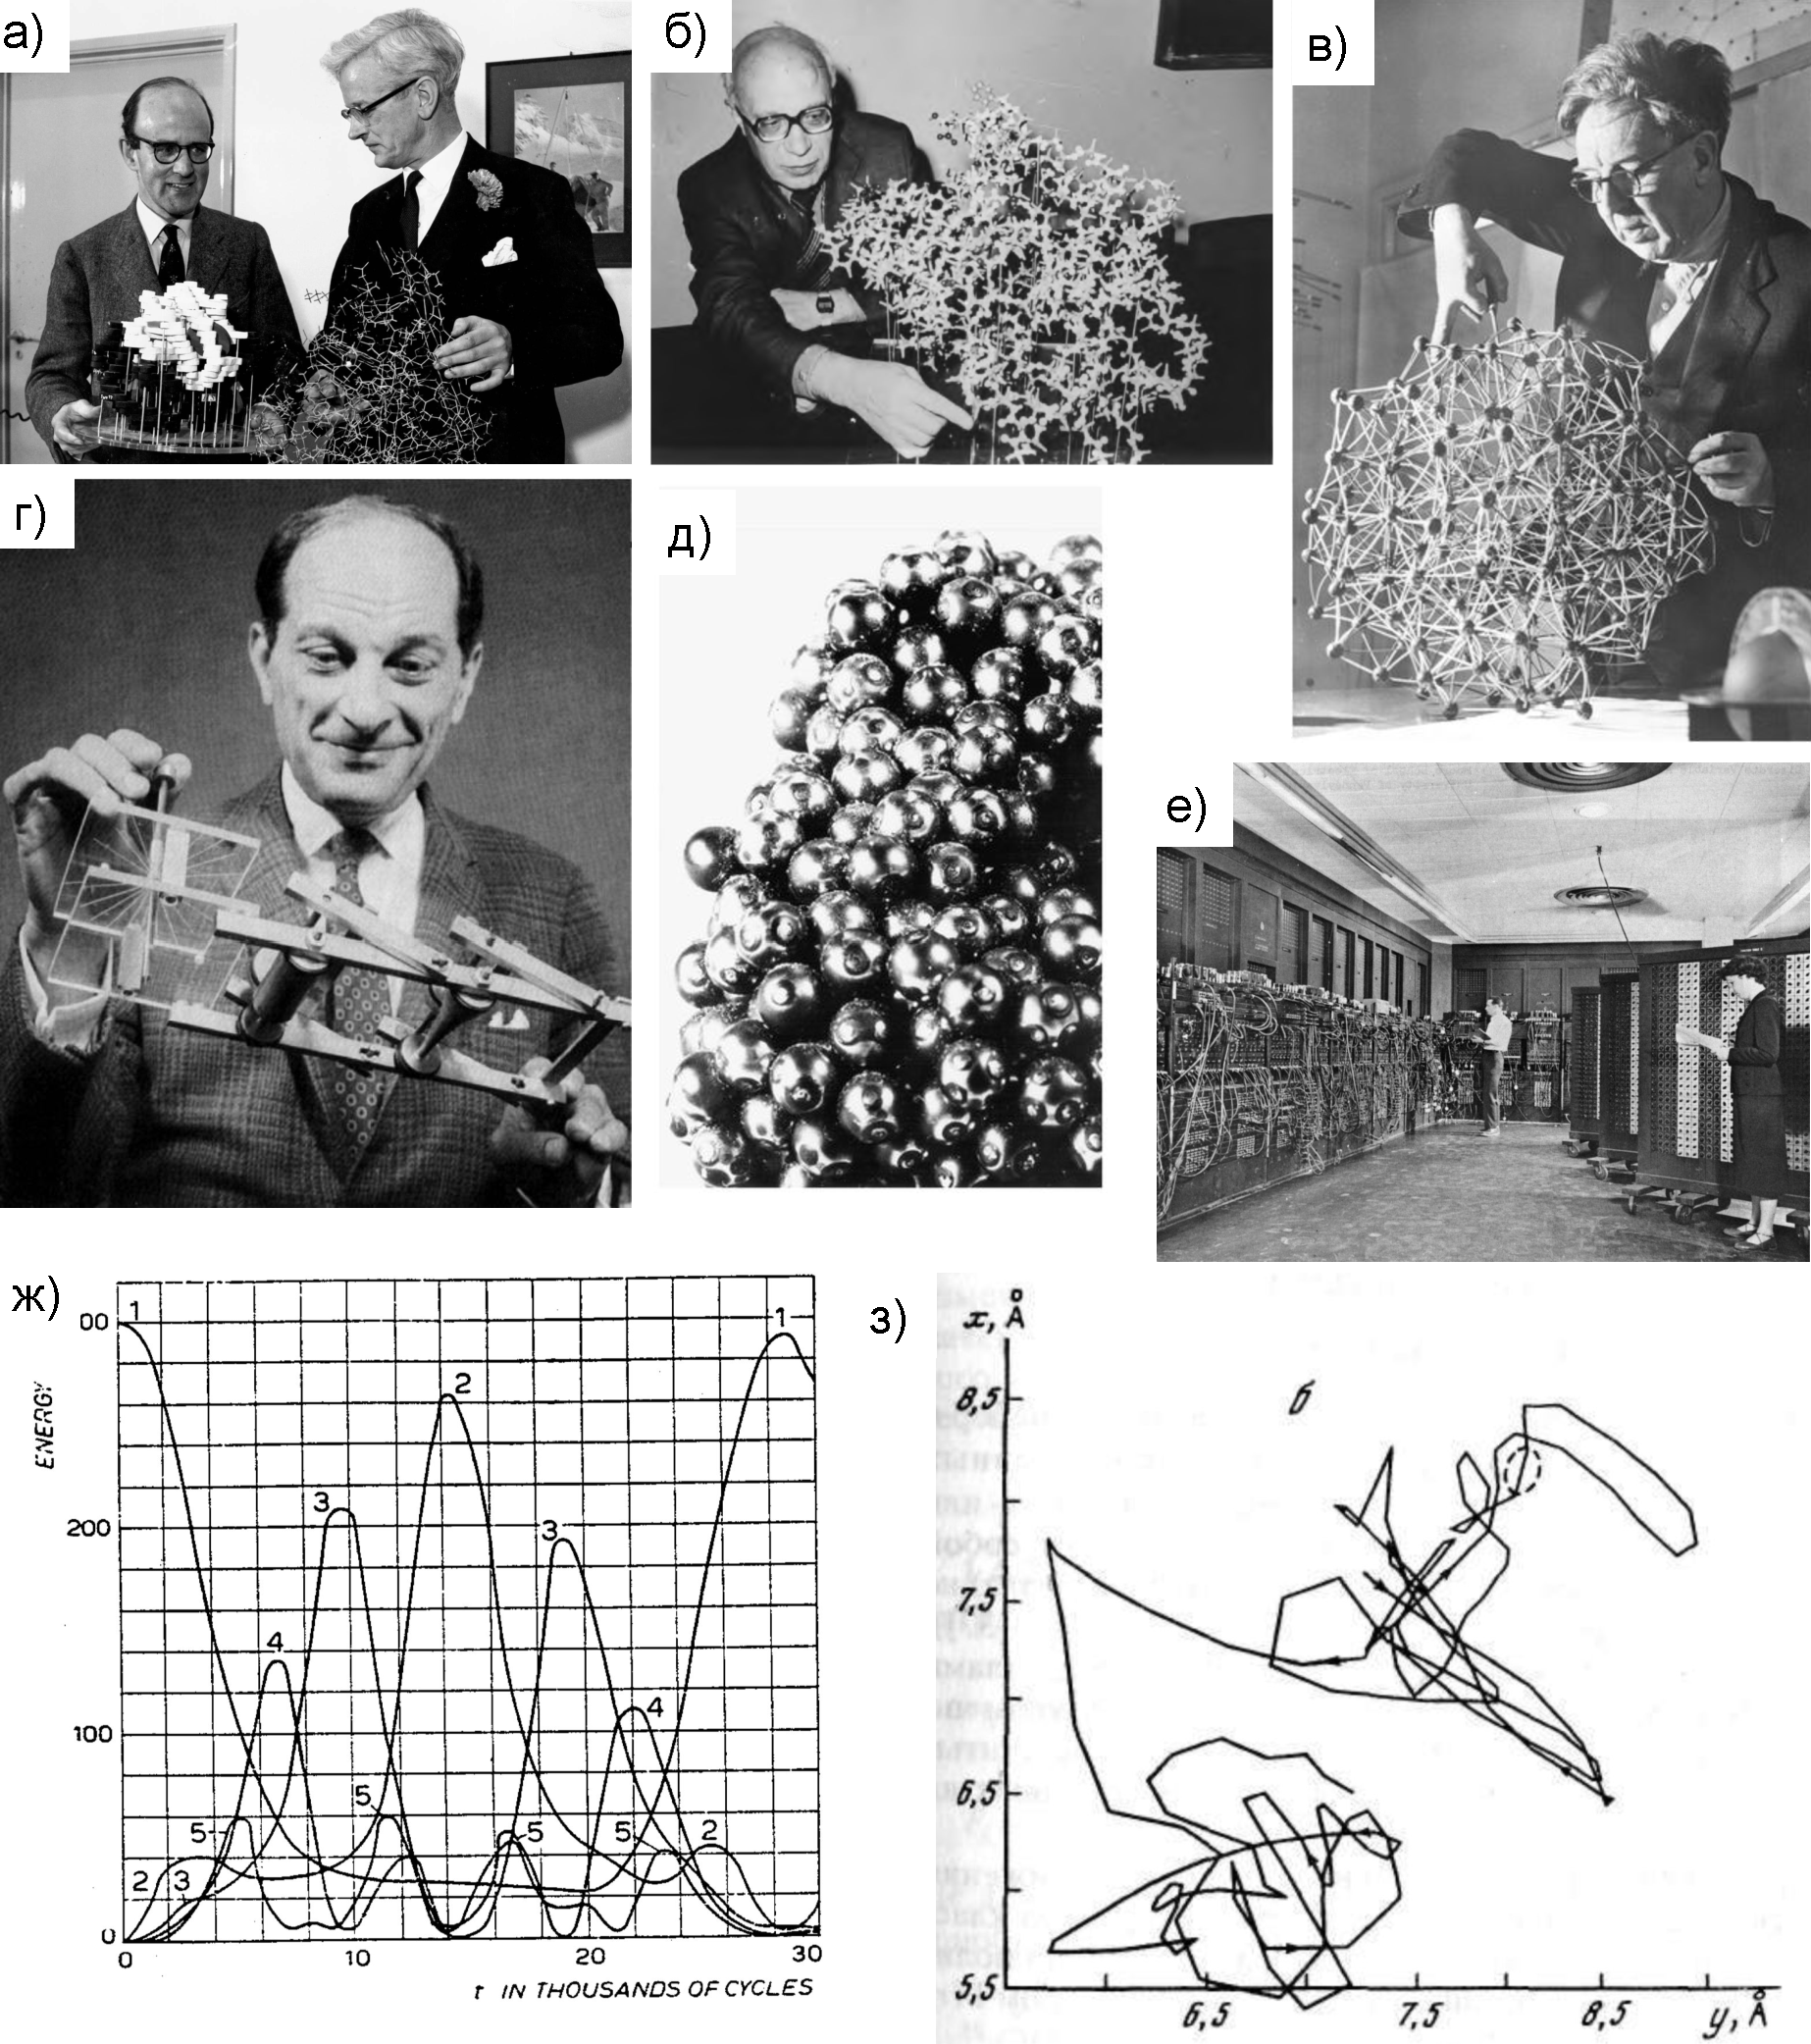
\includegraphics [width=350pt] {images/p1/mod_history.pdf}
  \caption[Иллюстрации к истории структурной биологии и моделирования.]{Иллюстрации к истории структурной биологии и моделирования. а) М. Перуц (слева) и Д. Кендрю (справа) со структурными моделями миоглобина. б) Б.К. Вайнштейн со структурой белка \cite{kovalchuk__2012}, в) Дж. Д. Бернал с моделью укладки атомов в жидкости \cite{finney_bernals_2013}, г) С. Улам с тележкой Монте-Карло Энрико Ферми \cite{gregg_mncp_nodate},  д) результаты физического моделирования жидкости в виде стальных шаров в работах Д.Д. Бернала \cite{finney_bernals_2013}, е) первый программируемый компьютер общего назначения ENIAC \cite{noauthor_english_1947}, ж) изменение полной энергии со временем для первых пяти мод вибрирующей струны в задаче Ферми-Пасты-Улама-Цингу, первая работа по исследованию статистических свойств механических систем методом молекулярной динамики, 1955 г. \cite{fermi_studies_1955}, (з) Траектории движения атомов в жидкости, рассчитанные методом МД из кандидатской диссертации А.Г. Гривцова, начало 1970-ых годов \cite{grivtsov_metodika_1996}.} 
  \label{fig:p1:mod_history}
\end{figure}

%%% ссылка на гривцова - обзорная статья маленкова https://www.google.com/url?sa=t&rct=j&q=&esrc=s&source=web&cd=&ved=2ahUKEwjrk6OPxcXrAhVI_SoKHTF5ACcQFjAAegQIBRAB&url=https%3A%2F%2Fistina.msu.ru%2Fdownload%2F101116065%2F1gBMHJ%3AYj-jpNMcPPBJ8nZ6Q-g4XcwGQIU%2F&usg=AOvVaw0_u1y_ZMajjPhNvAxlFsSa

%историческая статью о Монте Карло из LANL https://permalink.lanl.gov/object/tr?what=info:lanl-repo/lareport/LA-UR-88-9068
% а это статья метрополиса https://permalink.lanl.gov/object/tr?what=info:lanl-repo/lareport/LA-UR-88-9067
%также в вики неплохой обзор в биографии улама
%https://en.wikipedia.org/wiki/Stanislaw_Ulam#Manhattan_Project

%FERMIAC

%МД история
% https://en.wikipedia.org/wiki/Molecular_dynamics#History
% ферми улам (там картинка есть), затем Алдер, Раман (посмоьореть статьи)

% что-то из статьи гривцова - балабаева


Сам по себе термин \textit{молекулярное моделирование} (\textit{molecular modeling}) является достаточно широким понятием, значение которого постепенно расширяется и видоизменяется с развитием различных новых методов. В одних случаях упор может делаться непосредственно на задачу создания модели (например, пространственной модели белка), в других случаях на анализ и исследование свойств молекул на основе физических моделей поведения и взаимодействия атомов. К первому типу задач можно отнести традиционные задачи реконструкция структуры биомакромолекул по экспериментальным данным. Данный процесс всегда включает в себя шаг создания модели, которая удовлетворяет этим данным. На заре структурной биологии реконструкция биомолекул по результатам кристаллографических экспериментов долгое время сводилась к построению пространственных моделей из проволоки, дерева, других материалов (Рис. \ref{fig:p1:mod_history}aб). Позднее данный процесс был значительно автоматизирован с применением компьютерных технологий, разработаны соответствующие программные пакеты по автоматизации построения моделей и их визуализации (например, CCP4 \cite{winn_overview_2011}, O, Phenix \cite{liebschner_macromolecular_2019}, Coot  \cite{emsley_coot_2004}, Pymol \cite{schrodinger_pymol_2015}, Chimera \cite{pettersen_ucsf_2004}).  Построение моделей молекул в виде пространственного расположения атомов, удовлетворяющего набору экспериментальную данных, - одно из возможных значений термина компьютерное молекулярное моделирование. 
В то же время со времен возникновения молекулярно-кинетической теории (основы которой были в том числе заложены М.В. Ломоносовым \cite{lomonosov_sobranie_1950})
ученые стремились к описанию и предсказанию свойств молекулярных систем на основе учета взаимодействий между отдельными атомами, описываемых законами физики. В до-компьютерную эпоху такие предсказания можно было делать либо на основе теоретических расчетов, либо на основе физических механических моделей. Так, например, в 1950-60-ых годах для молекулярного моделирования жидкостей Джон Десмонд Бернал активно использовал механические модели в виде металлических и пластиковых шариков \cite{bernal_bakerian_1964}(Рис. \ref{fig:p1:mod_history}вд)\footnote{Любопытным также является факт, что тот же Дж. Д. Бернал является одним из основателей области биомолекулярной кристаллографии, под его руководством работали классики структурной биологии Макс Перутц, Дороти Ходжкин, Розалинд Франклин \cite{breathnach_desmond_1995}, а также в честь него назван пакет по молекулярному моделированию DESMOND \cite{kevin_schrodinger_2020}.}. С развитием компьютерных технологий появились возможности численного моделирования поведения молекулярных систем на основе их физических моделей. Следует отметить, что в английском языке для описания такого рода деятельности активно используется термин \textit{molecular simulations} (см. например \cite{Frenkel}), который на русский язык обычно переводится также ``молекулярное моделирование'', однако слово ``simulations'' имеет важные отличия в своей смысловой нагрузке. Под этим термином понимается не столько создание моделей, сколько изучение и анализ теоретических моделей с помощью вычислительных методов, так называемые ``вычислительные эксперименты''. В области инженерного моделирования в русском языке для обозначения термина ``simulation modeling'' используется термин \textit{имитационное моделирование}, однако он не вошел в обиход в среде исследователей, занимающихся молекулярным моделированием. Подход к изучению различных систем на основе проведения вычислительных экспериментов на данный момент многими воспринимается как одна из парадигм научного познания наравне с экспериментальным и теоретическими подходами \cite{hey_fourth_2009} и получил название \textit{in silico} подхода. В случае изучения свойств вещества данный подход предполагает наличие определенной физической модели исследуемого объекта, которая описывает взаимодействия между его составными частями, и использует различные вычислительные алгоритмы, чтобы исследовать свойства данной модели вещества. Если для описание физической модели вещества используются различные приближения, основанные на законах квантовой механики, то такие подходы зачатую называют \textit{ab initio} подходами (от лат. ``из первых принципов'' - подразумевая, что для моделирования необходимо знать лишь базовые физические константы). Для моделирования многих задач и веществ такой формализм является слишком вычислительно затратным, поэтому исторически область ``molecular simulations'' развивалась в первую очередь на основе формализма классической механики (частицы вещества представлялись в виде материальных точек, взаимодействующих по законам классической механики).

Зарождение области вычислительных экспериментов в молекулярном моделировании происходило в середине-конце 1940-ых годов во время работы над созданием ядерного и термоядерного оружия в США  и связано в первую очередь с именами Станислава Улама, Джона фон Неймана, Николаса Метрополиса, а также с вводом в строй в 1945 году первого электронного цифрового вычислителя общего назначения ENIAC (Рис. \ref{fig:p1:mod_history}е). С. Улам и Д. фон Нейман, работая над проблемой транспорта нейтронов в различных типах ядерных систем, предложили в 1947 году моделировать диффузию нейтронов путем многократного численного расчета траекторий движения отдельных нейтронов с учетом случайности их взаимодействия с окружающим веществом. Таким образом, решение задачи о вычислении средних характеристик данного процесса сводилось к статистической выборке (statistical sampling), а не к полному численному решению уравнений, которые описывали этот процесс. Благодаря наличию компьютера ENIAC  стало возможным написать компьютерную программу для соответствующих расчетов, которая использовала в том числе генератор псевдослучайных чисел для моделирования случайных событий и соответствующих статистических выборок \cite{eckhardt_and_1987}.  Подходы основанные на статистическом моделирования с использованием случайных величин были названы ими методомами Монте-Карло, по предложению Николаса Метрополиса, а первая статья по этому методу опубликована в 1949 году \cite{metropolis_monte_1949}. Любопытным является факт, что физик Энрико Ферми еще до формулировки метода Монте Карло Уламом и фон Нейманом использовал метод статистических выборок для своих задач, проводя расчеты вручную в предрассветные часы, когда страдал бессонницей \cite{metropolis_beginnig_1987}. В 1947 году, когда постановка расчетов на компьютере ENIAC была временно невозможной из-за его перевозки, Ферми придумал аналоговый компьютер, который можно было использовать для моделирования транспорта нейтронов. Данный компьютер представлял собой тележку с карандашом, которую нужно было передвигать по бумажному чертежу и периодически изменять ее направление на основе случайных чисел, таким образом моделируя передвижения нейтронов и их столкновения с атомами среды. Данное устройство получило название тележки Монте-Карло или FERMIAC (см Рис. \ref{fig:p1:mod_history}г).

Следующей важной вехой в развитии методов Монте Карло в молекулярном моделировании и статистической механике явилась разработка Метрополисом, супругами Розенблют и Теллер в 1953 году метода Монте Карло на основе марковских цепей (Markov Chain Monte Carlo, MCMC) для изучения уравнений состояния вещества состоящего из индивидуальных взаимодействующих молекул \cite{metropolis_equation_1953}. В этой работе авторы провели исследование двумерного газа из жестких сфер на компьютере MANIAC. Инновацией данного метода стало вычисление статистической выборки состояний согласно распределению Больцмана в многомерном пространстве через построение марковской цепи состояний. Случайные переходы между состояниями принимались или отклонялись согласно критерию Метрополиса-Хастингса таким образом, что лимитирующее распределение состояний в данной марковской цепи соответствовало Больцмановскому распределению состояний по энергиям. На идеях данной работы основано большинство подходов по моделированию молекулярных систем методами Монте Карло и в наши дни \cite{ivanov_methods_2009}.

1950-ые годы также ознаменовалось первыми работам в области применения метода молекулярной динамики - численного решения уравнений движения классической механики. 
Впервые Ферми, Паста, Улам и Цингу исследовали колебания струны с нелинейной упругостью и показали наличие необычной периодичности возникающей в нелинейных системах \cite{fermi_studies_1955}. 
Идея моделирования динамики молекулярных систем была сформулирована Олдером и Вайнрайтом в 1957 году -- с помощью компьютера UNIVAC исследовались фазовые переходы в системе твердых сфер \cite{alder_phase_1957}. К первым попыткам применить методы молекулярной динамики к реалистичным системам можно отнести работу Гибсона и др. 1960 года по моделированию радиационного поражения меди \cite{gibson_dynamics_1960} и работу Aнисура Рамана по моделированию жидкого аргона 1964 года \cite{rahman_correlations_1964}. В нашей стране первые шаги по развитию методов молекулярной динамики связаны с деятельностью А.А. Гривцова, Э.Э. Шноля, Н.К. Балабаева из Института прикладной математики (ИПМ, Москва) начиная с 1967 года \cite{grivtsov_metodika_1996}. С тех пор методы молекулярной динамики стали активно применяться для моделирования газов, жидкостей \cite{allen_computer_1989}, а  позднее стали активно применяться и для моделирования биомакромолекулярных систем. Развитие применения методов молекулярного моделирования к биомолекулярным системам связаны с деятельностью групп Мартина Карплуса, Арье Варшеля, Майкла Левитта, которые получили в 2013 году нобелевскую премию за ``разработку мультимасштабных моделей сложных химических систем'', а также групп Питера Коллмана, Хермана Берендсена, Клауса Шультена, Дэвида Кейса, Эрика Линдаля, Алекса МакКерела и др. Работы группа М. Карплуса легли в основу набора силовых полей CHARMM, a также одноименной программы для моделирования \cite{karplus_molecular_2003}. На основе подходов, силовых полей и программного кода CHARMM были развиты многие родственные программы, например, программа для параллельных расчетов молекулярной динамики NAMD (в группе К. Шультена) \cite{phillips_scalable_2020}, программа для моделирования на основе данных ЯМР XPLOR \cite{schwieters_xplor-nih_2003}, программа для моделирования по гомологии MODELLER \cite{sali_comparative_1993}. Работы группы Питера Коллмана положили основу программному пакету AMBER и одноименной группе силовых полей \cite{case_amber_nodate}. Работы группы Хермана Берендсена в Голландии заложили основы пакета по моделированию GROMACS \cite{lindahl_gromacs_2020} и силового поля GROMOS \cite{soares_improved_2005}. В нашей стране развитие программных продуктов в области молекулярной динамики связано в том числе с разработкой программы PUMA и ее версий под руководством Н.К. Балабаева \cite{likhachev_parallelism_2018}.

В первые десятилетия XXI века область молекулярного моделирования продолжала активно развиваться и совершенствоваться, в том числе и в методологическом плане. Стоит отметить адаптацию программного обеспечения для использования массивно-параллельных архитектур графических процессоров, что позволило уверенно проводить расчеты МД в микросекундном диапазоне не только на суперкомпьютерах, но и отдельных рабочих станциях \cite{noauthor_nvidia_nodate}.  Усилиями нескольких групп создавались специализированные компьютерные платформы для расчета молекулярной динамики, в частности архитектуры MD GRAPE в Японии \cite{ohmura_mdgrape-4_2014} и компьютеры ANTON компании D.E. Shaw Research \cite{shaw_anton_2014}. Последние позволяют проводить вычисления в миллисекундном диапазоне времен моделируемых систем.

Серьезный прогресс был достигнут и в совершенствовании методов повышения эффективности статистических выборок (enhanced sampling methods) в ходе расчетов молекулярной динамики. К таким методам можно отнести методы метадинамики (metadynamics) \cite{laio_escaping_2002}, адаптивной смещающей силы (adaptive biasing force) \cite{lesage_smoothed_2017}, адаптивно смещаемой молекулярной динамики (adaptevly biased molecular dynamics) \cite{marchi_adiabatic_1999}, динамики с обменом репликами (replica exchage molecular dynamic/parallel tempering) \cite{sugita_replica-exchange_1999}, управляемой молекулярной динамики (steered molecular dynamics) \cite{shaytan_neravnovesnaya_2006}. Многие из этих методов получили активное распространение благодаря созданию кросс-платформенного дополнения к пакетам молекулярной динамики PLUMED \cite{bonomi_promoting_2019}. Были в том числе развиты теоретические основы, связывающие характеристики расчета неравновесных молекулярных процессов с равновесными параметрами моделируемых системы. К таковым можно отнести равенство Джарзинского, связывающее работу в ходе неравновесного процесса над системой с разницей свободной энергии между конечным и начальным состояниями \cite{jarzynski_nonequilibrium_1997} и флуктуационную теорему Крукса (Crooks fluctuation theorem)\cite{crooks_entropy_1999}. Любопытно, что открытие и формулировка данных достаточно лаконичных и простых соотношений неравновесной статистической физики произошла только на рубеже XX и XXI веков, хотя явные предпосылки для их формулировки существовали со времен Больцмана. Отдельно стоит отметить развитие и успехи различных эмпирических подходов к моделированию структуры и дизайну белков. В отличие от методов, исходящих в первую очередь из физических представлений о структуре, подвижности и взаимодействии атомов в боимакромолекулах  (physics-based methods), такие подходы активно используют различные эмпирические скоринговые функции для оценки вероятности той или иной конформации белка, которые основываются на статистическом анализе большого количества уже известных пространственных структур белков, а также эволюционном анализе похожести различных аминокислотных мотивов в белках. Перебор конформационного пространства полипептидной цепи также зачастую ограничивают набором конформаций фрагментов присутствующих в уже известных структурах белков. К таким методам можно отнести подходы основанные на пакете ROSETTA \cite{leman_macromolecular_2020}, AWSEM-MD \cite{wu_awsem-idp_2018} и др.

Выше мы обсудили в историческом контексте различные взгляды на задачи и методы молекулярного моделирования. В одном случае речь идет о задачах поиска оптимальной пространственной модели молекулы на основе большого количества экспериментальных данных (например, реконструкции структуры белка по набору рефлексов картины дифракции его кристаллов), в другом случае упор делается на имитационное моделирования (molecular simulations) систем на основе физических моделей взаимодействий между атомами, которые иногда называют также \textit{ab inito} подходами (напр. \textit{ab initio protein folding}\footnote{Не стоит путать с пониманием термина \textit{ab initio} в квантовой химии, где под этим понимается моделирование на основе решения уравнения Шредингера.} и т.д.).
Разные аспекты данных подходов просуммированы на рисунке \ref{fig:p1:concept_matrix}, они отличаются по наличию, качеству и информационному содержанию используемых экспериментальных данных (Рис. \ref{fig:p1:concept_matrix}в), по используемым математическим подходам и физическим теориям (Рис. \ref{fig:p1:concept_matrix}б) и по самому представлению моделей (Рис. \ref{fig:p1:concept_matrix}а) - в одном случае речь обычно идет о некоторой статической структуре или наборе структур, в другом о статистических ансамблях различных конформаций.
% мнение Кейса про розетту https://onlinelibrary.wiley.com/doi/full/10.1002/cmr.a.21403


В то же время в структурной биологии существует большое количество задач, которые не решаются в рамках одного из двух вышеописанных подходов. С одной стороны для многих систем, экспериментальные данные могут присутствовать лишь в ограниченном количестве и зачастую иметь опосредованное отношение к деталям молекулярной структуры (напр. данные спектроскопических экспериментов, где оценивается взаимодействие введенных в структуру меток, данные по химической доступности и реакционной способности различных групп, данные малоуглового рассеяния и т.д.). С другой стороны, решение структурных задач напрямую \textit{in silico} методами физического моделирования на основе взаимодействия частиц невозможно для большинства систем в силу чрезвычайной вычислительной сложности и зачастую качества имеющихся моделей взаимодействия атомов в биомакромолекулах. Отдельную проблему представляют задачи описания структуры биомакромолекул, у которых нет явной статической структуры, а она представлена ансамблем конформаций. К примерам таких систем можно отнести внутренне разупорядоченные белки (англ. intrinsically disordered proteins), а также большинство биомакромолекулярных комплексов (вплоть до структуры хроматина на масштабах клеточного ядра) -- по мере роста размеров комплексов, они все реже формируют какую-то одну статическую конформацию, а их функционирование завязано сложную внутри- и межмолекулярную динамику. Для описания таких молекул динамический формализм используемый в имитационном молекулярном моделировании (molecular simulations) подходит значительно лучше, однако зачастую решение таких задач из первых принципов опять сводится к вышеописанным затруднением.

\begin{figure}[H] 
  \center
  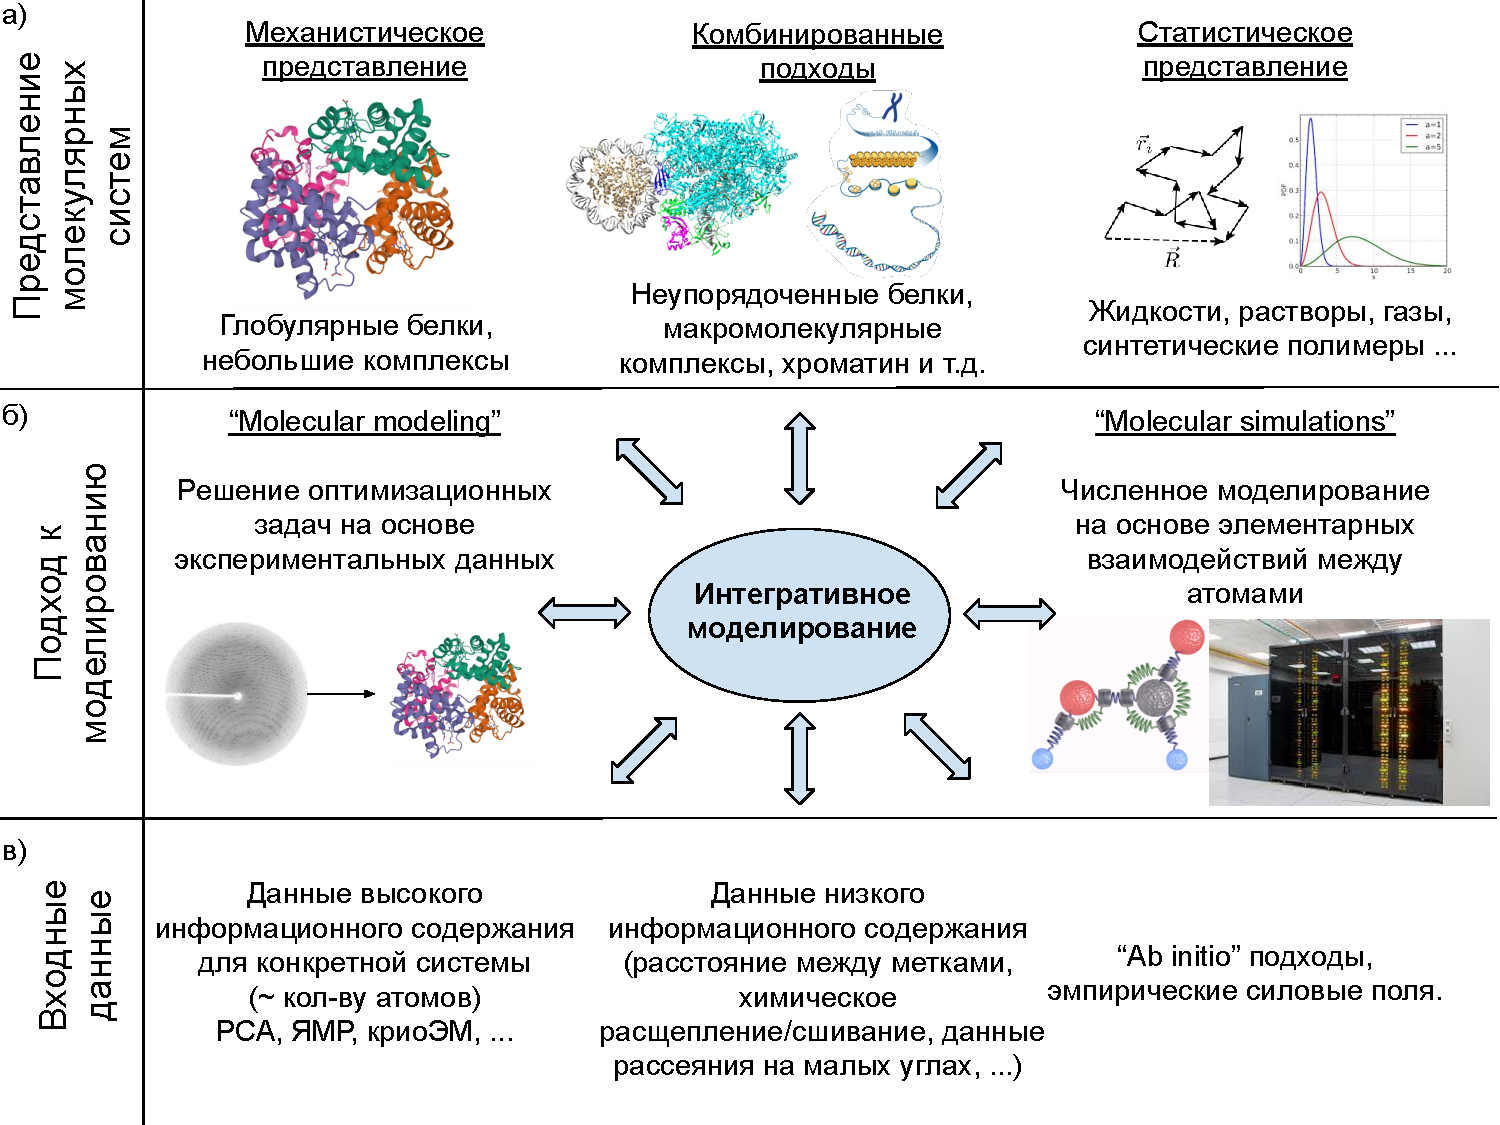
\includegraphics [width=\textwidth] {images/p1/concept_matrix.pdf}
  \caption{Диаграмма, суммирующая различные подходы к описанию, моделированию и изучению структуры и динамики биомакромолекул.} 
  \label{fig:p1:concept_matrix}
\end{figure}



Таким образом, актуальным является разработка гибридных методов и подходов по моделированию биомакромолекулярных комплексов, которые сочетают возможности построения структурных моделей как на основе экспериментальных данных (в том числе данных с низким информационным содержанием), так и на основе моделирования атом-атомных взаимодействий, а также учитывают структурные динамические особенности многих биомакромолекулярных систем. Такие подходы в последнее время в литературе получили название \textit{интегративного моделирования} (от англ. integrative modeling, см. напр. \cite{braitbard_integrative_2019}). Одной из задач интегративного моделирования является в том числе интеграция различного рода экспериментальных данных при построении моделей биомакромолекулярных систем. На Рис. 
\ref{fig:p1:int_mod} представлены различные типы экспериментальных данных, которые могут быть использованы в интегративном моделировании. К ним  могут относится структуры биомакромолекул или отдельных их частей полученные традиционными методами структурной биологии с высоким разрешением, а также набор данных низкого информационного содержания (когда данных недостаточно для реконструкции структуры традиционными методами), полученных различными биофизическими, биохимическими и другими методами. К последним могут относится данные полученные методами электронной микроскопии низкого разрешения, данные малоуглового рассеяния рентгеновских лучей или нейтронов, данные о взаимодействии введенных в структуру меток, получаемые методами ЯМР, ЭПР, спектроскопии Ферстеровского резонансного переноса энергии (FRET spectroscopy), данные по экспонированности в растворитель различных групп биомакромолекул, получаемые на основе экспериментов по дейтеро-водородному обмену, данные экспериментов по химическому сшиванию или разрушения биомакромолекул, данные получаемые с применением методов геномики (например, методов ChIP-seq, Hi-C и др.). Актуальной является и задача обратного рода -- имея некоторую структурно-динамическую модель биомакромолекулярной системы, рассчитать параметры ее отклика в различных типах экспериментов (см. Рис. \ref{fig:p1:int_mod}). Обсуждаемые подходы также важны при дизайне и конструировании новых биомакромолекулярных комплексов с полезными функциями.

Данная диссертационная работа посвящена развитию вышеописанных подходов интегративного моделирования. В работе представлены различные элементы интегративного подхода. В главе \ref{part2_supermd} рассмотрены работы по использованию суперкомпьютерных расчетов методом атомистической молекулярной динамики для изучения динамики биомакромолекулярных комплексов на основе уже известных пространственных структур, в главе \ref{part5_hrf} рассмотрены работы по интегративному моделированию нуклеосом на основе данных расщепления ДНК гидроксильными радикалами (hydroxyl-radical footprinting), в главе \ref{part6_nucl_complex} рассмотрены работы по созданию моделей комплексов нуклеосом с белками хроматина на основе разнообразных экспериментальных данных, в главе \ref{part4_amyloid} рассмотрены работы по интегративному моделирования амилоидоподобных фибрилл.

Последующие разделы данной главы будут посвящены изложению ряда методических основ методов молекулярного моделирования, которые использовались автором в ходе решения научных задач, излагаемых в данной диссертации, а также изложению основ некоторых экспериментальных методов, данные которых использовались автором в работах по интегративному моделированию биомакромолекулярных комплексов.



\begin{figure}[H] 
 \center
 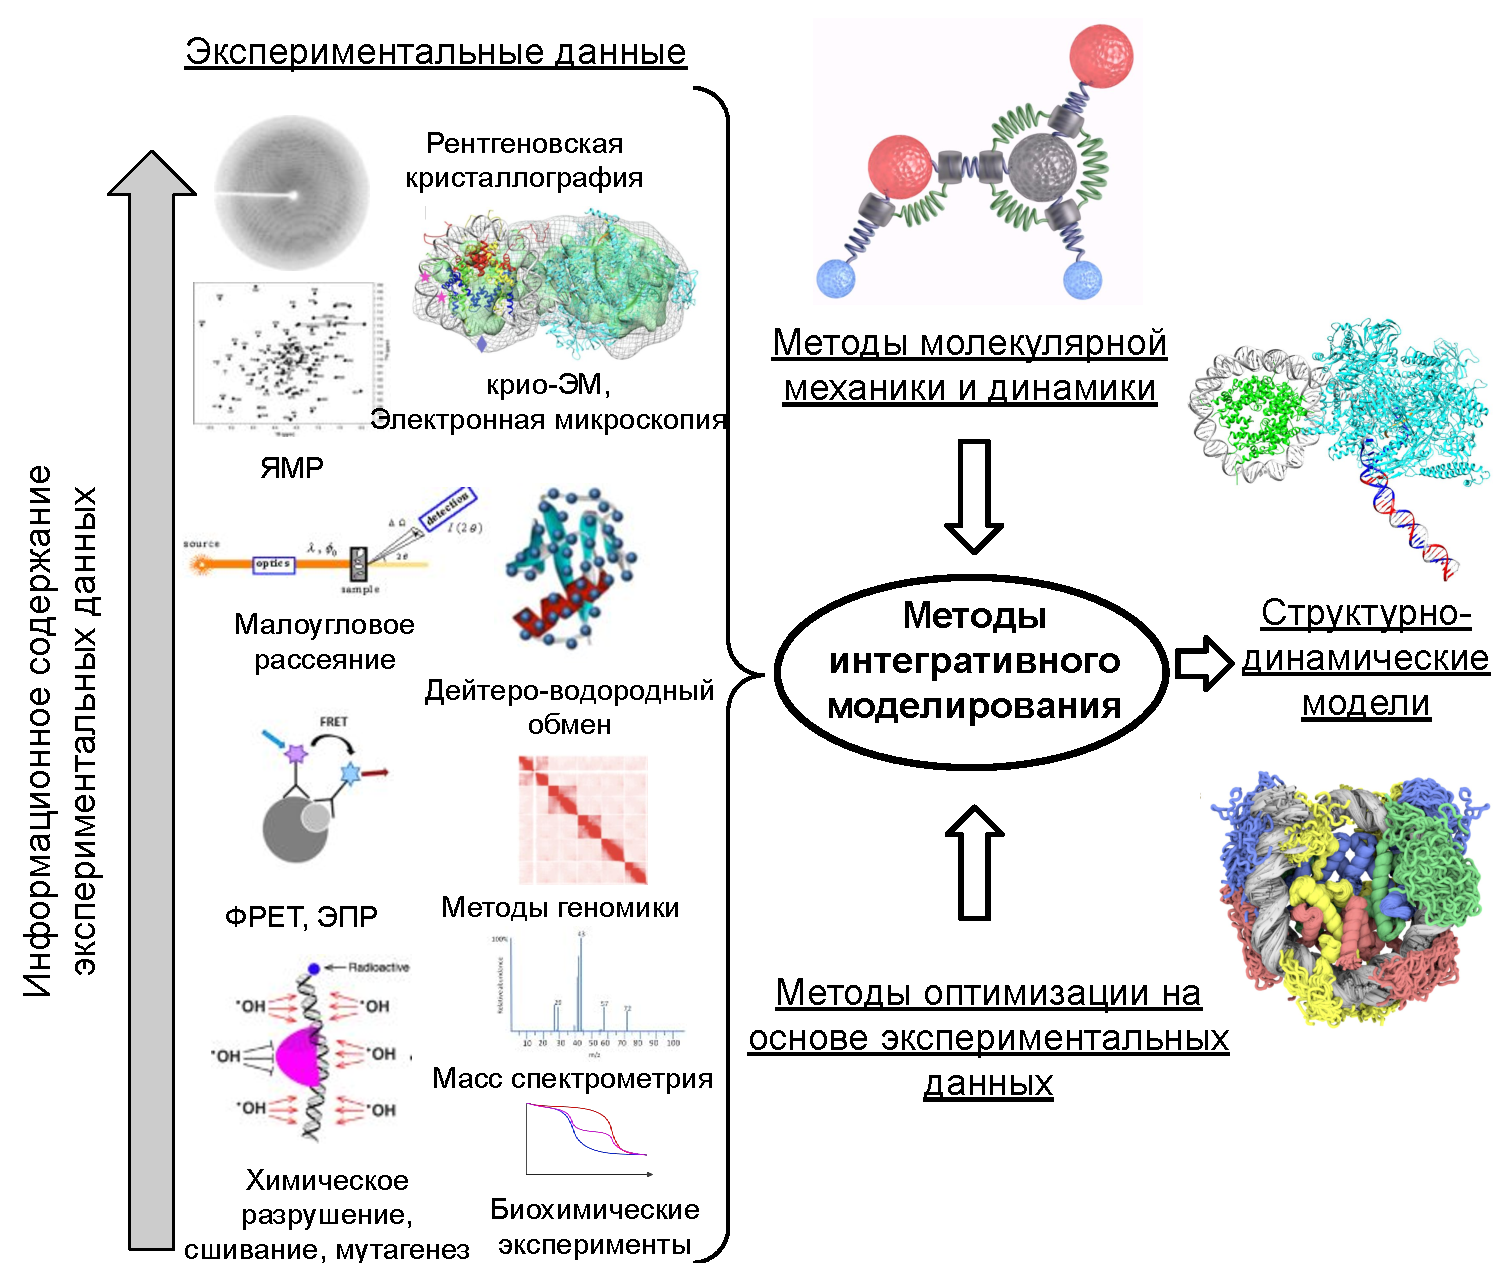
\includegraphics[width=\textwidth] {images/p1/int_mod.pdf}
 \caption{Идея методов интегративного моделирования.} 
 \label{fig:p1:int_mod}
\end{figure}



%Дальнейшая логика главы



% Методы молекулярной динамики и механики - взять из кфмн + добавить из немецкой
%расчет своб энергии - из кфмн
%мол поверхности из кфмн
% из диссертации армеева нужно взять про ДНК
% и про монте карло
%? что-то про метаД????
% Основы экспериментальных методов
%% ФРЕТ
%% Гидрокс
%% Электронка???
%%ЯМР???
%% Малоугл? (было ли в JMB)

%\section{Методы суперкомпьютерного атомистического моделирования } %%или \section{Методы молекулярной механики и динамики}
\section{Методы атомистического суперкомпьютерного моделирования} \label{part1_1_md}
\textit{Начало раздела \ref{part1_1_md} и раздел \ref{part1_1_md}.1 изложены согласно кандидатской диссертации автора \cite{shaytan_thesis_kfmn_2010} << }

О методах классического молекулярного моделирования написано множество подробных книг и монографий (см. например \cite{Frenkel,allen_computer_1989}), поэтому ниже мы лишь кратко обсудим основные понятия и подходы.

В основе методов классических атомистических методов молекулярного моделирования лежит представление о молекулярной структуре как о наборе классических частиц (материальных точек или в некоторых случаях твёрдых тел) взаимодействующих по законам классической механики. Молекулярно-механическая модель обычно предполагает следующие приближения: (i) электронные степени свободы не учитываются, а учитываются лишь атомные степени свободы, (ii) молекулы полагаются находящимися в основном энергетическом состоянии, (iii) автоматически предполагается приближение Борна-Оппенгеймера. На практике при задании конкретных типов взаимодействий между атомами в виде молекулярного гамильтониана предпринимается ещё ряд серьёзных приближений.

В случае моделирования биомолекулярных систем в приближении классической механики методические основы можно грубо разделить на три больших области: 1) задание механистической модели молекулярной системы на основе набора параметров, называемого силовым полем, 2) задание метода изучения динамики системы или метода изучения конформационного пространства данной системы, 3) различные технические и алгоритмические детали, связанные с эффективным и быстрым расчетом взаимодействий между атомами, а также оптимизацией расчетов на различных вычислительных системах.


%Ниже текст из файла materials/thesis_portable.pdf, ссылки надо смотреть там, но я их всех уже импортировал в зотеро.
%\todo{2S - из файла materials/thesis\_portable.pdf взять текст и картинки начиная со стр. 31 со слов "In molecular mechanics molecular system" до конца 39 страницы. с картинками и формулами. ссылки надо смотреть там, но я их всех уже импортировал в зотеро.}

\subsection{Силовые поля}
В молекулярной механике молекулярная система описывается в терминах классической механики набором точечных частиц (обычно представляющих атомы или группы атомов) и их взаимодействий, заданных функцией потенциальной энергии. Форма и структура функции потенциальной энергии называется силовым полем. На сегодняшний день разработано большое количество различных типов силовых полей, от обычных силовых полей до силовых полей, специфичных для определенного класса соединений. К наиболее популярным относятся группы силовых полей OPLS-AA \cite{jorgensen_development_1998}, AMBER \cite{cornell_2nd_1995}, CHARMM \cite{mackerell_all-atom_1998}, GROMOS \cite{schuler_improved_2001} , CVFF \cite{dauber-osguthorpe_structure_1988}, PCFF \cite{sun_force_1994}, MM3 \cite{allinger_molecular_1989} и другие. Эти силовые поля могут быть параметризованы относительно экспериментальных данных (в частности, калориметрических, спектроскопических), а также для воспроизведения поверхностей потенциальной энергии, вычисленных с помощью методов квантовой химии. Сложность функциональной формы силового поля может варьироваться, однако почти все молекулярные силовые поля содержат шесть общих основных термов для описания валентных и невалентных взаимодействий. Среди валентных взаимодействий выделяют термы описывающие растяжения ковалентных связей, деформации валентных углов, торсионных углов и ложноторсионные углы. Невалентные взаимодействия обычно описываются комбинацией парных ван-дер-Ваальсовых взаимодействий и кулоновских взаимодействий, основанных на точечных частичных зарядах атомов. Рисунок \ref{fig:p1_1:f10} и уравнение \ref{eq:p1_1:e1} дополнительно иллюстрируют эти термы. Многие из обычных силовых полей, используемых для моделирования биомолекул, включают в себя только упомянутые выше основные энергетические термины. Более сложные силовые поля (например, MM3, PCFF) могут также включать ангармонические члены и перекрестные члены для валентных взаимодействий, которые отражают связь между внутренними координатами. Например, при уменьшении валентного угла между атомами обнаруживается, что валентные связи удлиняются, чтобы уменьшить взаимодействие между атомами. Было обнаружено, что перекрестные члены играют важную роль в силовых полях, предназначенных для предсказания колебательных спектров  \cite{leach_molecular_2001}. Было высказано предположение, что наличие перекрестных членов (вместе с некоторыми другими особенностями) может обеспечить общий способ классификации силовых полей \cite{hwang_derivation_1994}. Согласно этой логике, силовое поле класса I ограничено гармоническими членами (например, для растяжения связей и валентного угла) и не имеет перекрестных членов. Силовое поле класса II будет иметь ангармонические члены и явные перекрестные члены для учета взаимоотношений между различными геометрическими параметрами. Еще одной характеристикой силового поля класса II считается возможность его использования без модификации одновременно для моделирования свойств изолированных малых молекул, конденсированных фаз и макромолекулярных систем \cite{leach_molecular_2001}.
\begin{multline}
    U(\{\vec{r}_i\})= \sum_{bonds} \frac{1}{2} k_b (l-l_0)^2  + \sum_{angels} \frac{1}{2}k_\theta (\theta - \theta_0)^2 + \sum_{torsions} \frac{1}{2} V_n [1+\cos({n\varphi-\varphi_0})] + \\
     \sum_{impropers} \frac{1}{2} k_\gamma (\gamma-\gamma_0)^2 + \sum_{j+1}^{N-1} \sum_{i=j+1}^{N} \Bigg\{ 4\epsilon_{ij} \Bigg[\Big(\frac{\sigma_{ij}}{r_{ij}}\Big)^{12} - \Big(\frac{\sigma_{ij}}{r_{ij}}\Big)^6\Bigg] + \frac{q_iq_j}{4\pi \epsilon_0 r_{ij}} \Bigg\} f_{ij}
     \label{eq:p1_1:e1}
\end{multline}

\begin{figure} [h!]
    \centering
    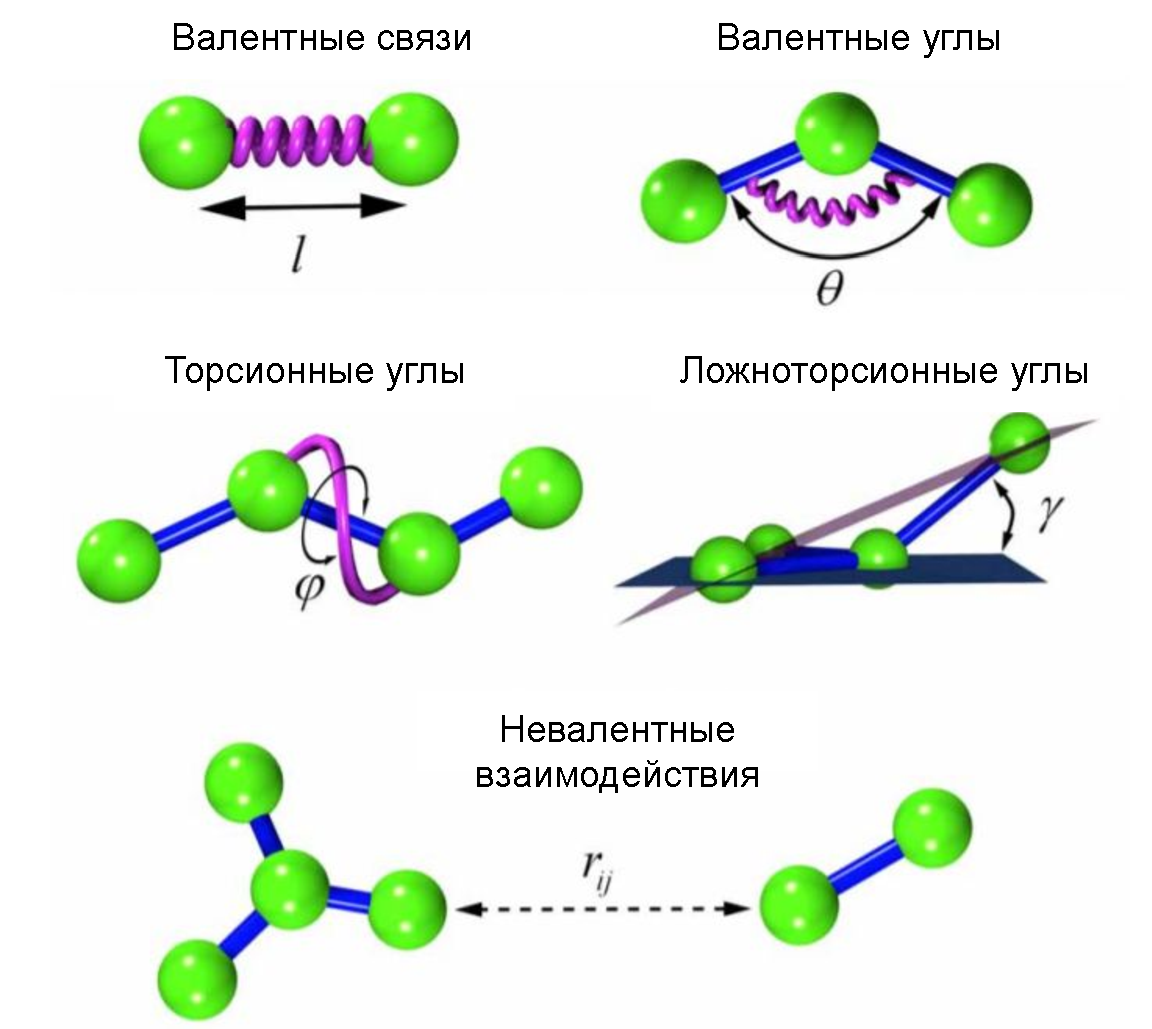
\includegraphics [width=\textwidth]{images/p1/part1_1_md/part1_1_md_f10.pdf}
    \caption[Энергетические термы силового поля]{Графическое изображение энергетических термов в силовых полях молекулярной механики. Атомы изображены зелеными сферами. Рисунок соответствует членам, представленным в уравнении 
    \ref{eq:p1_1:e1}}
    \label{fig:p1_1:f10}
\end{figure}


\subsubsection{Силовое поле OPLS-AA}
В качестве примера устройства типичного силового поля, применяемого для моделирования белков и других биологических молекул, рассмотрим поле OPLS-AA. Силовое поле OPLS-AA \cite{oplsaa,oplsaa2} является полноатомной версией поля OPLS (Optimized Potentials for Liquid Simulations), то есть атомы водорода рассматриваются явным образом. Параметры поля OPLS, в частности, подгонялись под экспериментальные свойства жидкостей, таких как плотность и теплота испарения.
Общая структура энергии молекулярной системы представлена в уравнении \ref{opls_ff_eqn}.

\begin{eqnarray}
&&U(r^N)=U_{bond}+U_{angle}+U_{dih}+U_{nb} \label{opls_ff_eqn}\\
&&U_{bond}=\sum_{bonds}K_r (r-r_{eq})^2\nonumber\\
&&U_{angle} = \sum_{angles} k_\theta \left ( \theta - \theta_{eq} \right )^2\nonumber\\
&&U_{dih} = \frac {V_1} {2} \left [ 1 + \cos \left ( \phi \right ) \right ] 
                + \frac {V_2} {2} \left [ 1 - \cos \left ( 2 \phi \right ) \right ] 
                + \frac {V_3} {2} \left [ 1 + \cos \left ( 3 \phi \right ) \right ] 
                + \frac {V_4} {2} \left [ 1 - \cos \left ( 4 \phi \right ) \right ]\nonumber\\
&&U_{nb}^{ab} = \sum_{i} ^{on\ a} \sum_{j} ^{on\ b} \left \{
                    4 \epsilon_{ij} \left [ \left( \frac {\sigma_{ij}}{r_{ij}} \right )^{12} 
                    - \left ( \frac {\sigma_{ij}}{r_{ij}} \right )^6 \right ]  + \frac {q_iq_j} {r_{ij}}
                   \right \} f_{ij}\nonumber
\end{eqnarray}
межмолекулярные взаимодействия $U_{nb}$ учитываются только для атомов, которые удалены на три и более связи, для 1-4 взаимодействий коэффициент скейлинга $f_{ij}=0.5$, во всех остальных случаях $f_{ij}=1$.

\subsubsection{Силовое поле PCFF}
Силовое поле PCFF (Polymer Consistent Force Field) \cite{pcff_sun_1994} основано на силовом поле CFF91 и относится к семейству силовых полей CFF (consistent force-field). Это поле создано для моделирования широкого класса органических полимеров, утверждается, что силовые поля второго поколения (к которым относится PCFF) более точно воспроизводят экспериментальные результаты, чем силовые поля первого поколения. Платой за это является более сложное устройство поля и наличие перекрёстных членов в функции энергии. Общий вид энергии молекулярной системы в приближении поля PCFF приведён в формулах \ref{pcff_eqn}. На Рис. \ref{fig:2_pcff_terms} приведено графическое пояснение к внутренним степеням свободы, являющимися параметрами для каждого члена потенциальной энергии.

\begin{eqnarray}
&&U(r^N)=U_{b}+U_{\theta}+U_{\phi}+U_{\chi}+U_{bb^\prime}+U_{\theta \theta^\prime}+U_{b\theta}+U_{b\phi}+U_{b^\prime \phi}+U_{\theta \phi}+U_{\phi \theta \theta^\prime}+U_{nb}  \nonumber \\
&&U_{b}=\sum_{b}K(b-b_0)^2\nonumber\\
&&U_{\theta}=\sum_{\theta}H(\theta-\theta_0)^2\nonumber\\
&&U_{\phi}=\sum_{\phi}V(1+\cos{(\phi-\phi_0)})\nonumber\\
&&U_{\chi}=\sum_{\chi}K_{\chi} \chi^2\nonumber\\
&&U_{bb^\prime}=\sum_{bb^\prime}F_{bb^\prime} (b-b_0)(b^\prime-b_0^\prime)\nonumber\\
&&U_{\theta\theta^\prime}=\sum_{\theta\theta^\prime}F_{\theta\theta ^\prime} (\theta-\theta_0)(\theta ^\prime-\theta _0^\prime)  \\  \label{pcff_eqn}
&&U_{b\theta}=\sum_{b\theta}F_{b\theta} (b-b_0)(\theta-\theta _0)\nonumber\\
&&U_{b\phi}=\sum_{b\phi}(b-b_0)[V_1\cos{\phi}+V_2\cos{2\phi}+V_3\cos{3\phi}]\nonumber\\
&&U_{b^\prime\phi}=\sum_{b^\prime\phi}(b^\prime-b^\prime_0)[V_1\cos{\phi}+V_2\cos{2\phi}+V_3\cos{3\phi}]\nonumber\\
&&U_{\theta\phi}=\sum_{\theta\phi}(\theta-\theta_0)[V_1\cos{\phi}+V_2\cos{2\phi}+V_3\cos{3\phi}]\nonumber\\
&&U_{\phi\theta\theta^\prime}=\sum_{\phi\theta\theta^\prime}K_{\phi\theta\theta^\prime}\cos{\phi(\theta-\theta_0)(\theta ^\prime-\theta _0^\prime)}\nonumber\\
&&U_{nb} = \sum_{i>j} \left \{ \left [ \frac { A_{ij} } { r_{ij}^9 } - \frac {B_{ij}} {r_{ij}^6} \right ]+ \frac{q_iq_j}  { r_{ij} } \right \} f_{ij}\nonumber
\end{eqnarray}

\begin{figure}[htbp]
  \centering
  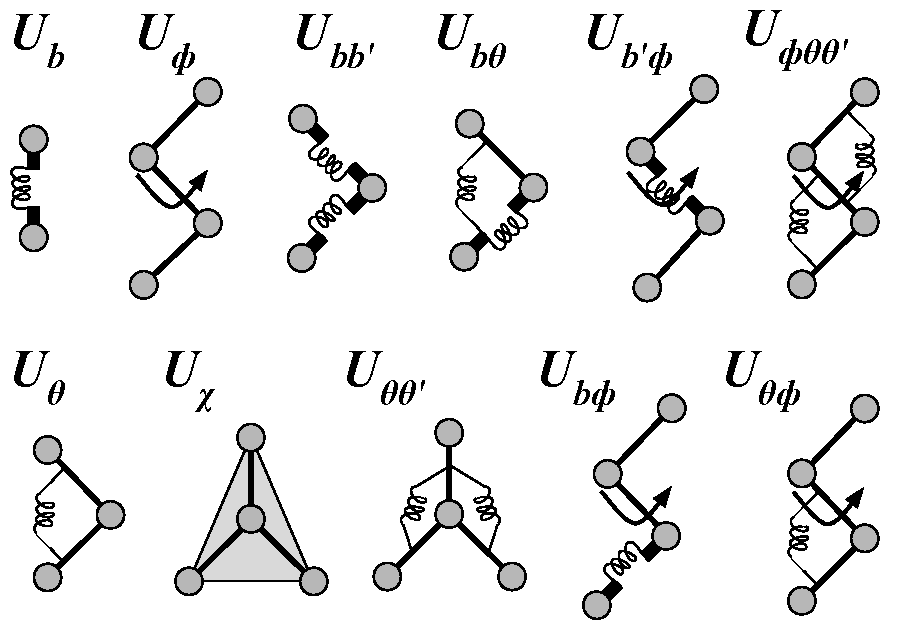
\includegraphics[width=15cm]{images/2_pcff_terms}
     \caption{Графическое пояснение к членам внутримолекулярной энергии уравнения \ref{pcff_eqn}.}
  \label{fig:2_pcff_terms}
\end{figure}

\textit{>>}

\subsection{Методы молекулярной динамики}

Определив модель молекулярной механики, можно применять различные методы для ее анализа; они включают в себя минимизацию энергии, моделирование молекулярной динамики, моделирование по методу Монте-Карло, а также различные более сложные методы, основанные на этих методах. Ключевым методом данной работы (а также, вероятно, наиболее часто используемым для изучения сложных молекулярных систем) является метод моделирования молекулярной динамики (МД) и его различных вариаций. Основная идея метода МД моделирования очень проста и основана на численном решении классических уравнений движения атомов в молекулярной системе на основе второго закона Ньютона:

\begin{equation}
    \frac{d^2 \overrightarrow{r_i}}{dt^2}= \overrightarrow{a}= \frac{\overrightarrow{F}}{m}= - \frac{1}{m_i} \nabla_i U(\textrm \{\vec{r_i}\})
\end{equation}
 
Численное решение обычно получается с помощью одной из схем интегрирования, такой как алгоритм Верле (velocity Verlet algorithm) \cite{swope_computer_1982}:

\begin{eqnarray}
    \overrightarrow{r}(t+\triangle t) = \overrightarrow{r}(t)+\overrightarrow{v}(t)\triangle t + \frac{1}{2} \overrightarrow{a}(t) \triangle t^2  \nonumber \\
    \overrightarrow{v}((t +\triangle t) =   \overrightarrow{v}(t) \frac{\overrightarrow{a}(t)+\overrightarrow{a}(t +\triangle t)}{2} \triangle (t)
\end{eqnarray}

Хотя основная идея, лежащая в основе МД-моделирования, на первый взгляд кажется довольно простой и понятной, ее обоснованность и интерпретация связаны с фундаментальными проблемами теоретической физики и математики на стыке механики, статистической физики и теории хаоса \cite{hoover_time_2001}. Одним из таких вопросов является связь между обратимыми во времени уравнениями Ньютона, используемыми для моделирования эволюции системы во времени, и эмпирическими необратимыми законами термодинамики, приводящими систему к состоянию, в котором энтропия максимальна.
    Другой набор вопросов и приближений, который имеет большое значение для практической реализации МД моделирования в реальных молекулярных системах, будет кратко обсужден ниже и включает использование периодических граничных условий, реализацию статистических ансамблей, динамику Ланжевена и диссипативных частиц, вычисления несвязанных взаимодействий, параллельная реализация МД алгоритмов.

\subsection{Периодические граничные условия}

Периодические граничные условия (ПГУ) - это метод, используемый для уменьшения влияния граничных эффектов на молекулярную систему во время моделирования и аппроксимации свойств объемных систем (таких как газы или жидкости) с помощью модели, состоящей из конечного набора молекул. Типичный случай применения периодических граничных условий - моделирование макромолекул в явном растворителе.
    В периодических граничных условиях ячейка моделирования окружена своими периодическими копиями во всех трех пространственных направлениях (см. Рисунок \ref{fig:p1_1:f11}), таким образом, эффективно образуя бесконечную кристаллическую структуру. Каждый атом, характеризуемый своими действительными координатами, также имеет координаты своих периодических образов. Распространенной формой учета частиц в периодических граничных условиях является соглашение о ближайшем образе, при котором каждый отдельный атом в системе взаимодействует с ближайшим к себе образом каждой частицы в системе.

\begin{figure} [h!]
    \centering
    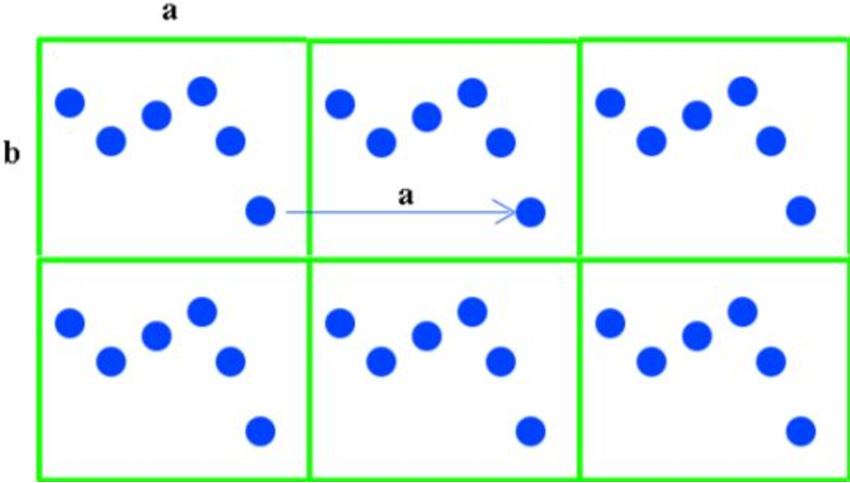
\includegraphics [width=\textwidth]{images/p1/part1_1_md/part1_1_md_f11.pdf}
    \caption[Иллюстрация периодических граничных условий]{Иллюстрация периодических граничных условий, используемых в МД моделировании. Кружками обозначены атомы и их периодические образы в соседних периодических ячейках.}
    \label{fig:p1_1:f11}
\end{figure}

ПГУ также используются в сочетании с методами учета электростатических взаимодействий на больших расстояния, такими как суммирование по Эвальду \cite{sagui_molecular_1999}. Поэтому полный электростатический заряд системы должен быть равен нулю, чтобы избежать проблем с расхождением значений полной электростатической энергии. Однако даже если система нейтральна, общий дипольный момент ячейки может приводить к некоторым искусственным энергетическим эффектам, похожим на пироэлектрические эффекты в полярных кристаллах.
Чтобы предотвратить артефакты связанные с ПГУ, размер ячейки моделирования должен быть достаточно большим, чтобы избежать таких нефизических эффектов. В том числе если размер ячейки слишком мал, макромолекула может взаимодействовать со своим собственным изображением в соседней ячейке, что эквивалентно взаимодействию молекулы с собой. Это может привести к нефизической динамике большинства макромолекул.

\subsection{Статистические ансамбли в МД моделировании}

Настоящие молекулярные системы никогда не изолированы от окружающей среды. Взаимодействие молекулярной системы с окружающей средой в плане обмена энергией, объемом и частицами с точки зрения статистической физики может быть описано в терминах статистических ансамблей \cite{landau_statistical_2000}. Ансамбль микросостояний молекулярной системы, связанной с внешним термостатом с постоянной температурой, называется каноническим ансамблем (или NVT-ансамблем), аналогично система под поршнем, связанная с термостатом, дает изобаро-изотермический ансамбль (или NPT -ансамбль).

    Поскольку базовые алгоритмы МД моделирования обеспечивают решение уравнений движения для изолированной системы (микроканонический ансамбль), обычно вводятся специальные алгоритмы, которые имитируют связь системы с внешним резервуаром энергии или объема \cite{frenkel_understanding_2002}. Цель таких алгоритмов - поддерживать правильные характеристики средней температуры (объема), в то же время обеспечивая правильную величину колебаний, которые зависят от внутренних свойств системы, таких как теплоемкость и сжимаемость.
    Среди алгоритмов термостатирования следующие алгоритмы нашли применение в современных кодах моделирования: термостат Берендсена \cite{berendsen_molecular_1984}, термостат Нозе-Гувера \cite{hoover_canonical_1985}, цепи Нозе-Гувера \cite{martyna_nose-hoover_1992}, термостат Андерсена \cite{andersen_molecular_1980}, термостат решкалирования скоростей \cite{bussi_canonical_2007}.
    
    Термостат Берендсена, будучи самым простым, полагается на масштабирование скоростей с коэффициентом $\lambda$  на каждом временном шаге:
\begin{equation}
   \lambda= \sqrt{\Big[1+\frac{\triangle t}{\tau_t} \Big\{\frac{T_0}{T}-1  \Big\} \Big]}
\end{equation}
    Влияние этого алгоритма на температуру заключается в том, что фактическая температура корректируется до эталонной температуры $T_0$ экспоненциальным образом:
\begin{equation}
    \frac{dT}{dt}= \frac{T_0 - T}{\tau}
\end{equation}
Однако термостат Берендсена имеет серьезные недостатки: во-первых, он не допускает колебаний температуры и, таким образом, не реализует правильный ансамбль, и, во-вторых, было показано, что процедура перемасштабирования скорости вызывает ``эффект летающего куба'' при моделировании системы в вакууме, когда энергия связанная с поступательным движением и вращением всей системы непрерывно растут, в то время как энергия высокочастотных основных мод истощается \cite{harvey_flying_1998,golo_dynamic_2002}.
    Формализм Нозе-Гувера - это подход, основанный на расширенном лагранжиане, содержащем дополнительные искусственные координаты и скорости, который приводит к детерминированной молекулярной динамике при постоянной температуре. Расширенный гамильтониан, первоначально предложенный Нозе \cite{nose_molecular_1984}, можно записать следующим образом:
\begin{equation}
    H_{Nose}= \sum_{i=1}^{N} \frac{\tilde {\mathbf p}_{i}^{2}}{2 m_i \tilde s^2} + U (\tilde r^N) + \frac{\tilde {\mathbf p}_{s}^{2}}{2Q} + g k T_0 ln(\tilde s)
\end{equation}
    где ${\mathbf p}_s$ и s - координаты расширенной переменной, Q - ее фиктивная масса, k - постоянная Больцмана, $T_0$-эталонная температура, g - параметр. Этот гамильтониан порождает микроканонический ансамбль из 6N + 2 степеней свободы. Переменные, присутствующие в этом гамильтониане, называются виртуальными переменными. Тем временем определяется набор реальных переменных, которые соотносятся с виртуальными переменными следующим образом:
\begin{eqnarray}
    {\mathbf r}= \tilde {\mathbf r} \\
    {\mathbf p}= \tilde {\mathbf p} /s \\
    s= \tilde s \\
    dt=d \tilde t / s
\end{eqnarray}
    и псевдогамильтониан может быть тогда задан как 
\begin{equation}
    H({\mathbf p},{\mathbf r})= \sum_{i=1}^{N} \frac{{\mathbf p}_{i}^{2}}{2m_i}+ U({\mathbf r}^N)
\label{pseudoH}
\end{equation}
Можно показать, что микроканонический ансамбль, сгенерированный путем решения уравнений движения для расширенной системы в виртуальных переменных, будет соответствовать канонической выборке реальных переменных согласно соответствующему псевдогамильтониану (\ref{pseudoH}), если параметр g = 3N и другие условия выполнены (см. ниже). Тепло передается в реальную систему и обратно от расширенной переменной колебательным образом, что приводит к почти периодическим колебаниям температуры. 
    Позже Нозе и Гувер показали, что соответствующие уравнения движения могут быть сформулированы в терминах реальных системных переменных, что дает уравнения движения Нозе-Гувера:
\begin{eqnarray}
    \ddot{{\mathbf r}_i} = \frac{{\mathbf F}_i}{m_i} - \frac{\xi \dot{{\mathbf r}_i}}{m_i} \nonumber \\
    \dot{\xi}= \frac{kg}{Q}(T(t)-T_0)
\end{eqnarray}

    Детальный теоретический анализ негамильтоновой динамики, генерируемой уравнениями Нозе-Гувера, показывает, что алгоритм генерирует правильное распределение только при наличии единственного интеграла движения, сохраняющегося во время динамики, обычно полной энергии расширенной системы, и никаких других интегралов движения \cite{frenkel_understanding_2002}. Исключением является сохранения полного импульса системы, если центр масс остается неподвижным.
    
    Данное утверждение также подразумевает, что динамика является эргодической, то есть усреднение по траектории эквивалентно усреднению по фазовому пространству. Однако было показано, что для небольших или жестких систем динамика неэргодична, и правильные распределения не генерируются. Чтобы решить эту проблему, Martyna et al. \cite{martyna_nose-hoover_1992} предложили схему, в которой термостат Нозе-Гувера соединен с другим термостатом или цепочкой термостатов.
    
    В подходе Андерсена к изотермическому моделированию система связана с термостатом с помощью стохастических импульсных сил, которые время от времени действуют на случайно выбранные частицы. В процессе столкновения частицы приобретают новые скорости согласно распределению Максвелла-Больцмана, соответствующие заданной температуре. Термостат Андерсена обеспечивает правильный статистический ансамбль, но делает динамику прерывистой из-за случайных столкновений.
    
    Термостат решкалирования скорости (Velocity rescale), предложенный Bussi et al. \cite{bussi_canonical_2007} представляет собой комбинацию термостата Берендсена со стохастическим членом, который обеспечивает правильное распределение кинетической энергии.
    
    
    Аналогично алгоритмам термостатирования существуют алгоритмы баростатирования, которые позволяют реализовать правильное целевое давление и NPT ансамбль. Схема баростатирования Берендсена \cite{berendsen_molecular_1984} позволяет быстро отрелаксировать систему до целевого давления и поддерживать его на протяжении всего моделирования. Алгоритм Берендсена изменяет масштаб координат и векторов ячейки моделирования на каждом шаге с помощью матрицы $\mu$ при заданном эталонном давлении $P_o$ следующим образом:
\begin{equation}
    \hat{\mu}_{ij}= \delta_{ij} - \frac{\triangle t}{3 \tau_p} \beta_{ij} \big\{P_{0ij}-P_{ij}(t)\big\}
\end{equation}
Где $\beta$ - изотермическая сжимаемость.
    Это приводит к экспоненциальной релаксации давления в соответствии с законом:
\begin{equation}
    \frac{dP}{dt}=\frac{P_0 -P(t)}{\tau_p}
\end{equation}
Как и в случае с термостатом, баростат Берендсена не полностью реализует NPT ансамбль и подавляет правильные флуктуации давления и объема, однако, если эти флуктуации не являются термодинамически значимыми, данный подход является простым и удобным методом поддержания постоянного давления в системе.

    Другой схемой поддержания давления, аналогичной термостату Нозе-Гувера, которая правильно реализует NPT ансамбль, является схема  Парринелло-Рамана \cite{parrinello_polymorphic_1981}.

\subsection{Ланжевеновская и диссипативная динамика частиц}
    Ланжевеновская (или стохастическая) динамика и диссипативная динамика частиц (ДДЧ) (dissipative particle dynamics) - это методы, которые позволяют имитировать влияние растворителя на динамику молекулярной системы посредством введения диссипативных и стохастических членов в уравнения движения. Взаимодействие диссипативных и стохастических сил не только изменяет динамику, но также может гарантировать правильные характеристики NVT ансамбля. В пределе небольшого воздействия (малая вязкость растворителя) эти методы также являются удобными алгоритмами для поддержания NVT ансамбля при моделировании методом МД.
    
    
    Стохастическая или скоростная динамика Ланжевена добавляет трение и шум к уравнениям движения Ньютона следующим образом:
\begin{equation}
   m_i \ddot{{\mathbf r}}={\mathbf F}_i - m_i \xi_i \dot{{\mathbf r}} + \hat{{\mathbf r}_i}
   \label{eq:p1:langevin}
\end{equation}
    где $\xi_i$ - постоянная трения, а $\hat{r_i}(t)$ - это шумовой процесс с корреляционной функцией
\begin{equation}
   \big  \langle \hat{r}_{i}^{\alpha}(t)\hat{r}_{i}^{\beta}(t+s) \big \rangle = 2m_i \xi_i kT \delta(s) \delta_{ij} \delta_{\alpha\beta}
   \label{eq:p1:lang_proc}
\end{equation}
т.е. он нескоррелирован для разных частиц, разных компонентов и разного времени. Формальный вывод уравнения Ланжевена посредством редукции быстрых степеней свободы и их аппроксимации двумя последними членами уравнения (\ref{eq:p1:langevin}) основан на технике проекционного оператора, введенной Мори и Цванцигом \cite{zwanzig_nonequilibrium_2001}. В остальном члены, отвечающие за трение и стохастический процесс, имеют интуитивно понятный физический смысл: первая представляет собой диссипативную силу, вызываемую трением с растворителем, вторая - своего рода движущую силу, которая вызывается ``ударами'' окружающих частиц растворителя.

Случайное трение и стохастические силы не сохраняют ни импульс, ни энергию системы. Под действием силы трения энергия отводится из системы, в то время как стохастический процесс может закачивать энергию в систему, поэтому динамика и выборка больше не соответствуют микроканоническому ансамблю, в то время как энергия системы флуктуирует, что напоминает канонический ансамбль NVT. Кроме того, можно показать, что для реализации распределения Больцмана в стохастической динамике трение и стохастические силы должны быть связаны через уравнение (\ref{eq:p1:lang_proc}).
        
Хотя метод Ланжевена привлекателен для жидкостных систем, где структура растворителя не важна, или как алгоритм для строгой реализации ансамбля NVT, он не дает правильной гидродинамики, поскольку случайные силы и силы трения не сохраняют импульс системы. Чтобы преодолеть эту проблему, но при этом сохранить положительные черты стохастической динамики, метод диссипативной динамики частиц (ДДЧ) (dissipative particle dynamics) был первоначально разработан Хугербрюгге и Кольманом для мезоскопического моделирования простых и сложных жидкостей \cite{hoogerbrugge_simulating_1992}. В ДДЧ сила, действующая на каждую частицу, состоит из трех членов \cite{moeendarbary_dissipative_2009}:
\begin{equation}
    {\mathbf F}_i= \sum_{j \neq i} ({\mathbf F}_{ij}^{C} + {\mathbf F}_{ij}^{D} +{\mathbf F}_{ij}^{R})
\end{equation}
консервативная сила, диссипативная сила и случайная сила, соответственно. В то время, как консервативная сила является обычной парной силой, диссипативная и случайная силы определяются следующим образом:
\begin{equation}
   {\mathbf F}_{ij}^{D} = -\gamma \omega_D (r_{ij})({\mathbf n}_{ij} \cdot {\mathbf v}_{ij}) {\mathbf n}_{ij}
\end{equation}
\begin{equation}
   {\mathbf F}_{ij}^{R}= \sigma \omega_R (r_{ij}) \zeta_{ij} {\mathbf n}_{ij}
\end{equation}
где $r_{ij}= |{\mathbf r}_i -{\mathbf r}_j|$j, ${\mathbf n}_{ij}= {\mathbf r}_{ij}/|{\mathbf r}_{ij}|$, $\gamma$ и $\sigma$ - скалярные параметры, представляющие силу трения и случайную силу. $\omega_D$ и $\omega_R$ - весовые коэффициенты, которые варьируются от 0 до 1 и исчезают выше радиуса отсечки $R_c$. $\zeta_{ij}$ - представляет собой гауссовский белый шум со следующими свойствами:
\begin{equation}
   \big\langle \zeta_{ij}(t) \big\rangle = 0, \zeta_{ij}=\zeta_{ji}
\end{equation}
\begin{equation}
    \big\langle \zeta_{ij}(t) \zeta_{i' j'}(t') \big \rangle= \big( \delta_{ii'}\delta_{jj'}+\delta_{ij'}\delta_{i'j} \big) \delta(t-t')
\end{equation}
Замечательной особенностью уравнений ДДЧ в отличие от динамики Ланжевена является то, что
диссипативные и случайные силы зависят только от относительного положения и скорости
частицы и действуют по векторам, соединяющим пары частиц. Это в сочетании с
симметрией индексов обеспечивает выполнение третьего закона Ньютона и сохранение количества движения. Далее можно показать, что уравнения ДДЧ описывают
системы в ансамбле NVT при $\sigma^2 = 2\gamma kT$. Выбор одной весовой функции может
быть произвольным, однако можно показать, что обе функции должны быть связаны как
$\omega_D (r) = (\omega_R (r))^2$.
Типичный выбор для этой функции:
\begin{equation}
    \omega (r)= \Bigg\{ 2 \bigg(1- \frac{r}{R_c}    \bigg), r \leq R_c  ;   0, r > R_c\Bigg\}
\end{equation}
ДДЧ в основном применяется как метод мезоскопического моделирования, где частицы ДДЧ представляют собой целые молекулы или области жидкости, а не отдельные атомы. Однако трение и случайные члены могут также использоваться в атомистическом моделировании для моделирования влияния растворителя и реализации ансамбля NVT. Преимуществами термостата ДДЧ перед термостатом Ланжевена является сохранение импульса и малый радиус взаимодействий ДДЧ, оба фактора способствуют крупномасштабным конформационным переходам в молекулярной системе, если они должны произойти.

\subsection{Расчет невалентных взаимодействий}
    Вычисление невалентных взаимодействий и особенно кулоновских взаимодействий - одна из задач МД моделирования. Важной отличительной чертой электростатических взаимодействий является их медленный затухающий характер $(\sim 1/r)$, что, строго говоря, делает некорректным обрезку электростатического взаимодействия на некотором расстоянии во время вычисления сил и энергии при моделировании. В трехмерной объемной системе энергия взаимодействия точечной частицы с окружающей средой, характеризуемой плотностью заряда $\rho (r)$, была бы выражена интегралом:
\begin{equation}
   E= \iiint \frac{\rho (\vec{r})}{|\vec{r}- \vec{r}_0|} d^3 \vec{r}
\end{equation}
    который может сходиться только условно. Таким образом, необходимо соблюдать особую осторожность при расчете электростатических взаимодействий в моделировании МД. Было показано, что при простой обрезке кулоновских взаимодействий могут возникать серьезные артефакты, особенно при моделировании систем зарядов, начиная от шума и нестабильности при моделировании и заканчивая неблагоприятным воздействием на молекулярный порядок \cite{sagui_molecular_1999}.
    Если изучаемая система не является периодической (т.е. не используются периодические граничные условия), единственной альтернативой полному расчету электростатических взаимодействий (что для больших систем является недопустимо дорогостоящим, поскольку масштабируется как $\sim N^2)$ является их обрезка на некотором расстоянии Rc. Однако необходимо обосновать отсутствие серьезных побочных эффектов в таком случае. Наиболее распространенные ошибки могут возникать из-за: (i) отсутствия непрерывности силы, особенно при образовании нескомпенсированных зарядов на длине радиуса обрезания, приводящего к алгоритмическому шуму и тепловыделению, (ii) для заряженных систем и систем с внутренней периодичностью энергия и поведение системы могут зависеть от радиуса обрезания причудливым образом.
    
    В системах, которые используют периодические граничные условия, может использоваться альтернативная более надежная стратегия суммирования электростатических взаимодействий, она основана на методе суммирования Эвальда и родственных алгоритмах PME (particle mesh Ewald) и PPPM (particle-particle particle-mesh Ewald), основанные на интерполяции функций по значениям в узлах сеток \cite{frenkel_understanding_2002}. Идея суммирования по Эвальду состоит в том, чтобы заменить бесконечную медленно сходящуюся сумму электростатического взаимодействия данного набора частиц и всех их периодических образов двумя быстро сходящимися суммами, одна в прямом, а другая - в обратном пространстве. Рассмотрим представление набора точечных зарядов, дополненных гауссовыми функциями экранирования и их обратными функциями на рисунке \ref{fig:p1_1:f12}.

\begin{figure} [h!]
    \centering
    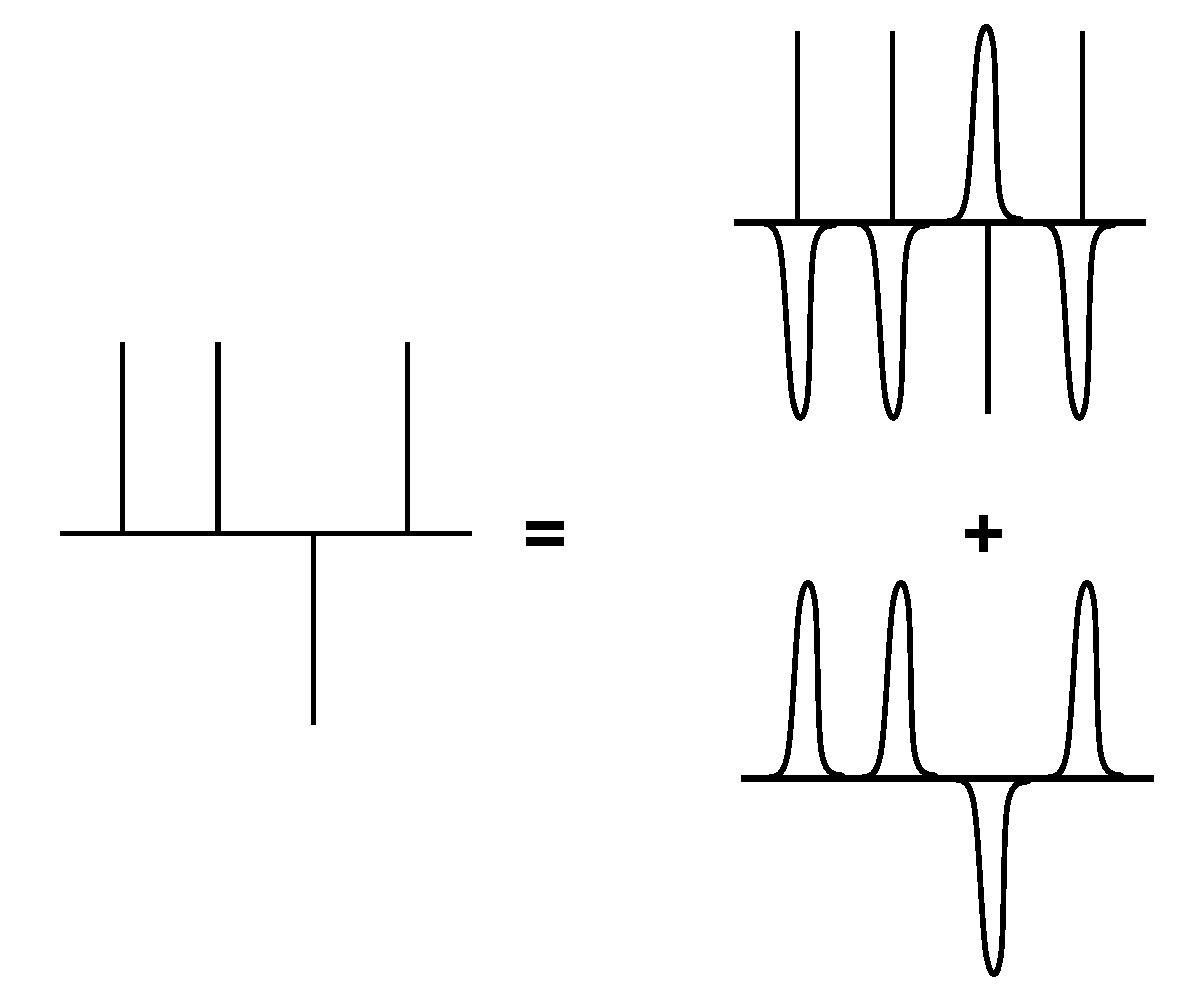
\includegraphics [width=\textwidth]{images/p1/part1_1_md/part1_1_md_f12.pdf}
    \caption{Схематическое изображение разложения заряда, используемого в суммировании по Эвальду.}
    \label{fig:p1_1:f12}
\end{figure}

    Гауссовские экранирующие функции имеют вид:

\begin{equation}
    \rho_{Gauss}(r)= -q_i(\alpha/\pi)^{3/2} exp(-\alpha r^2)
\end{equation}
    Можно показать, что в этом случае полный электростатический потенциал может быть выражен как сумма потенциалов обеих подсистем, представленных на рисунке \ref{fig:p1_1:f12}, за вычетом члена энергии самовзаимодействия. Электростатический потенциал экранированных точечных зарядов быстро спадает и может быть суммирован в прямом пространстве, в то время как потенциал компенсирующей подсистемы (плавно меняющиеся периодические гауссианы) можно легко вычислить в обратном пространстве Фурье на основе решения уравнения Пуассона. Результирующая полная энергия системы может быть записана следующим образом:
\begin{equation}
    U= \frac{1}{2} \sum_{i \neq j}^{N} \frac{q_i q_j \erfc{(\sqrt{\alpha}r_{ij})}}{r_{ij}} + \frac{1}{2V} \sum_{k \neq 0}\frac{4 \pi}{k^2} |\rho ({\mathbf k})|^2 exp(-k^2 / 4\alpha) - (\alpha/ \pi)^{1/2} \sum_{i=1}^{N} q_{i}^{2}
\end{equation}
    где $\rho ({\mathbf k}) \equiv \sum_{i=1}^{N} q_i exp(i{\mathbf k} \cdot {\mathbf r}_i)$, V - объем периодической ячейки.

    Однако сумма Эвальда требует больших вычислительных ресурсов для больших систем с порядком масштабирования  $O(N^{3/2})$ и остается дорогостоящей по сравнению с традиционными схемами обрезки взаимодействий. Чтобы решить эту проблему, были разработаны подходы на основе интерполяционных сеток, все они пытаются ускорить решение уравнения Пуассона в периодических граничных условиях, используя преимущества быстрого преобразования Фурье (БПФ) для вычисления дискретных преобразований Фурье \cite{sagui_molecular_1999}. Эти методы могут масштабироваться как $O(N log (N))$.
    Методы суммирования, подобные суммированию по Эвальду, могут вычислять электростатическую энергию в периодической системе с заданной точностью. Их использование привело к значительному повышению стабильности при моделировании биомолекул. Однако, некоторые фундаментальные проблемы моделирования все еще существуют и могут привести к артефактам во время моделирования \cite{sagui_molecular_1999}. Смит и Петтитт \cite{smith_ewald_1996,smith_presence_1997} изучали динамические артефакты, вызванные суммированием по Эвальду. Они сосредоточились на вопросе о величине энергетических барьеров при свободном вращении диполей в системах с периодичностью (наличием дальнего порядка). Представьте себе единственный идеальный диполь в начале элементарной ячейки, который затем периодически воспроизводится в соседних ячейках. Потенциальная энергия системы будет зависеть от ориентации диполя, что не подходит для исследования растворов биомолекул. Однако Смит и Петтитт показали, что вращательные барьеры незначительны для дипольных молекул в растворителях с высокой диэлектрической проницаемостью при комнатной температуре с типичными размерами ячейки моделирования. Для моделирования в растворителях с низкой диэлектрической проницаемостью или в вакууме отсутствие артефактов не может быть гарантированно.






% \subsection{Методы молекулярной динамики}
% Задача молекулярной динамики фактически заключается в решении классических уравнений движения для системы с заданным гамильтонианом. Решение уравнений движения реализуется численно с помощью разностных схем таких, как алгоритм Верле или Лип-Фрог алгоритм. Важной особенностью ``хороших'' алгоритмов является обратимость во времени и сохранение объёма фазового пространства. Известно также, что алгоритм Верле обладает ``теневой'' характеристикой, то есть точки траектории, получаемые посредством этого алгоритма, точно соответствуют (конечно, за исключением ошибки численного округления) некоторой ``теневой траектории'' механической системы, которая однако не проходит, через точку с начальными условиями. Иными словами, алгоритм Верле генерирует траекторию, которая соответствует экстремуму действия для некоторой ``теневой траектории'' (\cite{Frenkel} разд. 4.3.5).

% Для решения проблемы поверхностных эффектов в методе МД применяют периодические граничные условия. Особое внимание в последнее время обращается на тот факт, что при использовании периодических условий необходимо использовать решёточные алгоритмы для учёта дальнодействующих взаимодействий, таких как электростатические, поскольку обрезание зарядовых взаимодействий может приводить к артефактам моделирования. На данный момент хорошо разработаны достаточно быстрые решёточные алгоритмы учёта электростатики такие, как методы PME и PPPM.

% Отдельной проблемой является задание ансамблей в методе молекулярной динамики. Для задания распределения по температуре существует два принципиальных подхода: стохастическая и негамильтонова динамика. В стохастическом подходе в уравнения движения вводятся случайные члены (например, такие как в уравнении Ланжевена), которые позволяют привести статистическое распределение точек МД траектории к каноническому ансамблю. Подход негамильтоновой динамики был предложен Гувером \cite{Hoover}, он разработал такую модификацию уравнений движения, в которой предельным для точек фазового пространства является каноническое распределение. Однако в оригинальном алгоритме Нозе-Гувера были найдены проблемы при некоторых условиях, и на данный момент наиболее надёжным считается алгоритм цепей Нозе-Гувера.




%\section{Методы расчета свободной энергии в молекулярном моделировании}
%\section{Методы расчета свободной энергии взаимодействия с растворителем в молекулярном моделировании}

Предположим, что молекулярная система характеризуется некоторым Гамильтонианом, зависящим от параметра: $H(\lambda)$. \textit{Будем говорить, что каждому значению $\lambda$ соответствует некоторое $\lambda$-состояние системы.} Каким образом возможно рассчитать разницу в свободной энергии меду двумя $\lambda$-состояниями?\\

Начиная с 1960-х годов для практической реализации в численных экспериментах широкое применение получили такие методы, как \textit{метод термодинамического интегрирования}, \textit{метод возмущения свободной энергии}, \textit{метод Беннетта}. С появлением работ  Джарзинского, Крукса, Шёртса и др. \cite{jarzinski,crooks,stanford_ben} выявилась более глубокая связь между этими методами. Соотношения неравновесной статистической физики, выведенные Джарзинским (Jarzinsky equality) и Круксом (transient fluctuation theorem) предлагают более общий подход к решению задачи отыскания свободной энергии через неравновесные процессы. При этом, упомянутые ранее методы являются частными случаями в этом общем подходе, но могут также быть получены независимыми способами.
В данной работе нам будут интересны эти три метода, так как они имеют широкое практическое применение.
\subsection{Метод термодинамического интегрирования}
Метод ТИ может быть получен из простых соображений. Свободная энергия Гиббса системы задаётся в общем случае выражением \ref{gibbsFE}.
\begin{equation}
G=-kT\ln\int \exp\left(-\frac{H(V,\vec{p},\vec{q},\lambda)+PV}{kT}\right)d\vec{p}d\vec{q}dV
\label{gibbsFE}
\end{equation}
Для метода ТИ основным является равенство \ref{TI_equal}.
\begin{equation}
\frac{\partial G}{\partial \lambda}=\left\langle \frac{\partial H}{\partial \lambda} \right\rangle
\label{TI_equal}
\end{equation}
И разница свободной энергии между разными $\lambda$-состояниями даётся выражением \ref{TI}.
\begin{equation}
\Delta G=\int \frac{\partial G}{\partial \lambda} d\lambda
\label{TI}
\end{equation}

Метод достаточно эффективен и часто применяется. Однако, необходимость интегрирования функции $\frac{\partial G}{\partial \lambda}$ требует достаточно большого количества вычислений и вносит дополнительную ошибку численного интегрирования, которую трудно оценить при ограниченном наборе известных значений функции.

\subsection{Метод возмущения свободной энергии} 
В методе возмущения свободной энергии (Free energy perturbation - FEP) разница свободной энергии между разными $\lambda$-состояниями может быть записана в виде \ref{fep_equal}, что и определяет метод отыскания разницы свободной энергии между двумя состояниями.
\begin{equation}
\Delta G=-kT \ln{\frac{\int dV\vec{p}d\vec{q}\exp \left \{ -\frac{H(V,\vec{p},\vec{q},\lambda_1)+PV}{kT} \right \}}{\int dV\vec{p}d\vec{q}\exp \left \{ -\frac{H(V,\vec{p},\vec{q},\lambda_0)+PV}{kT} \right \}}}=-kT
 \ln{<\exp{\frac{H_0-H_1}{kT}}>_0}
\label{fep_equal}	
\end{equation}
где $H_0=H(V,\vec{p},\vec{q},\lambda_0)$, $H_1=H(V,\vec{p},\vec{q},\lambda_1)$, усреднение ведётся по NPT-ансамблю соответствующему состоянию системы с $\lambda=\lambda_0$.

\subsection{Метод Беннетта}
Метод Беннетта (Bennett acceptance ratio method) позволяет наиболее эффективным образом комбинировать данные, получаемые при прямом и обратном процессе. Иными словами, мы переводим систему из состояния с $\lambda=\lambda_0$ в состояние с $\lambda=\lambda_1$ и при этом получаем некоторое значение работы $W_F$. Однако возможен и обратный процесс перевода системы из состояния $\lambda_1$ в состояние $\lambda_0$ с работой $W_R$. В 1976 году метод был предложен Беннеттом \cite{bennet} как обобщение метода FEP. Однако в настоящее время стало ясно, что таким образом можно обобщить практически любые методы расчёта свободной энергии. Этот \textit{обобщённый метод Беннетта} основывается на соотношениях Крукса и позволяет построить наилучшую статистику (оценочную функцию максимального правдоподобия) для оценки значения свободной энергии по наборам параметров $W_F$ и $W_R$ (см. \cite{stanford_ben}).\\

В простейшем случае как обобщение метода FEP метод Беннета (оригинальная работа \cite{bennet}, 1976 год) имеет следующий вид.
Итак, допустим, что у нас есть набор работ по бесконечно быстрой трансформации системы из состояния $\lambda_0$ в состояние $\lambda_1$ - ${W_F}$, и обратно - ${W_R}$. Метод Беннета задаёт оценочную функцию, которая определяет значение разницы свободной энергии с минимальной дисперсией среди всех оценочных функций.
Оценочная функция задаётся неявно, как решение уравнения \ref{beneq} по параметру $C$.

\begin{equation}
\label{beneq}
\sum _m^{N_R} f(W_R^m+C)=\sum _n^{N_F} f(W_F^n-C)
\end{equation}
В уравнении (\ref{beneq}) $f$-функция Ферми-Дирака:
$$
f(x)\equiv \frac{1}{1+\exp{\beta x}}
$$
$N_F$ и $N_R$ - соответственно количество полученных замеров в прямом и обратном направлениях, $\beta=1/kT$. Можно показать, что наилучший результат всегда достигается при $N_F\approx N_R$. Более того, метод Беннета имеет преимущество перед простым методом FEP. Так, более эффективным является осуществление выборки значений работы в прямом и обратном направлениях, и затем применение метода Беннета, чем осуществление в два раза большей выборки в одном направлении и применении метода FEP.

\subsection{Методы расширенных ансамблей}
Кроме трёх вышеприведённых методов развиваются и более современные методы расширенных ансамблей. В этих методах происходит одновременное моделирование систем при различных значениях параметра $\lambda$ и между этими состояниями осуществляются переходы, как в методе Монте-Карло. Хорошим примером адаптивного метода расширенных ансамблей является работа \cite{lyubartsev_2004}. Однако, на данный момент программное обеспечение, реализующее такие методы, мало распространено.

%Методы расчета молекулярных поверхностей
\section{Методы расчета поверхностей в молекулярном моделировании} \label{part1_3_sasa}
\textit{Раздел \ref{part1_3_sasa} изложен согласно кандидатской диссертации автора \cite{shaytan_thesis_kfmn_2010} << }
Поверхность доступная растворителю (ПДР) (solvent accessible surface area (SASA)) -- это поверхность биомолекулы, которая доступна растворителю. Обычно ПДР выражают с квадратных ангстремах. ПДР была впервые описана Ли и Ричардсом\cite{lee_richards} и иногда называется молекулярной поверхностью Ли-Ричардса, она определяется как поверхность которую описывает центр пробной сферы при ``обкатывании'' сферы вокруг молекулы. Размер сферы обычно берётся порядка размера молекулы воды. В этом плане ПДР можно воспринимать, как расширенную поверхность Ван-дер-Ваальса.

Кроме ПДР широкое распространение получила поверхность Коннолли, которая представляет собой как бы полость, которая формируется в растворителе при помещении в него молекулы. Коннолли разработал также полуаналитический метод расчёта такой поверхности \cite{connolly_1983}.

На Рис. \ref{f:2_surf} изображены поверхности доступные растворителю и молекулярные поверхности Коннолли для модельной системы.

\begin{figure}[htbp]
   \centering
   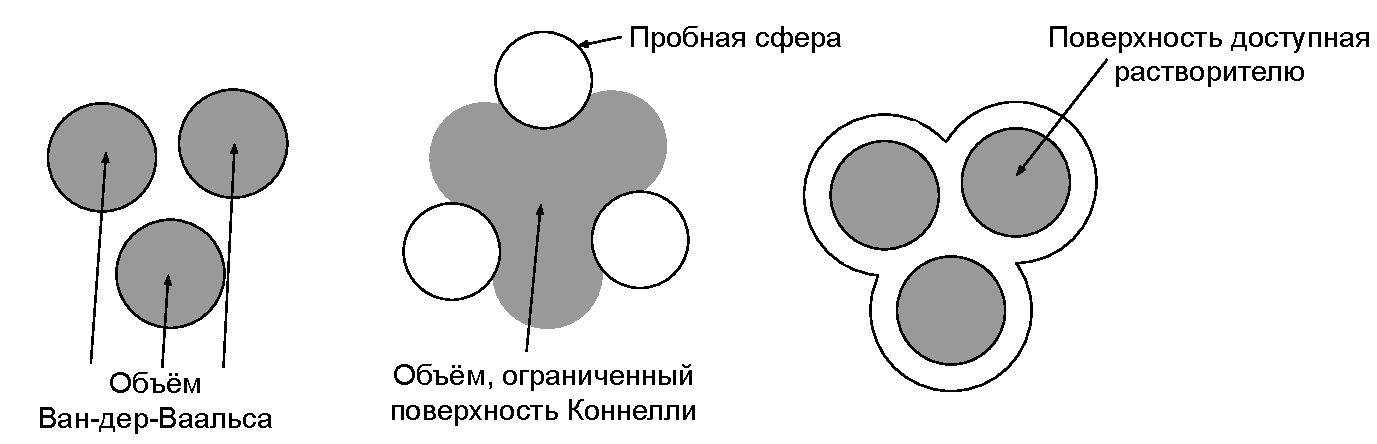
\includegraphics[width=15cm]{images/2_surf}
      \caption{Пояснения к определению поверхности доступной растворителю и поверхности Коннолли.}
   \label{f:2_surf}
\end{figure}
\textit{>>}

%\section{Методы моделирования ДНК в динуклеотидном приближении}
\section{Методы моделирования ДНК в динуклеотидном приближении}

Описание конформации ДНК в виде набора геометрических параметров, определяющих взаимное расположение соседних нуклеотидных пар относительно друг друга, может использоваться как для исследования структуры ДНК, так и для создания физических моделей гибкости ДНК. Последние могут быть встроены в алгоритмы интегративного моделирования ДНК и ДНК-белковых комплексов. В данном разделе излагаются представления о  параметрах геометрии ДНК, эмпирических силовых полях для описания энергии изгиба ДНК в динуклеотидном приближении, а также программные продукты и методы моделирования, включая разработки научной группы автора.

\subsection{Описание геометрии ДНК}
Планарность азотистых оснований нуклеотидов и относительная планарность комплементарных пар оснований в двухцепочечной спирали ДНК позволяет применить для описания их взаимного расположения математический формализм, в котором основания или пары оснований представлены в виде плоских элементов с двумя уникальными гранями, отличимыми друг от друга из-за асимметрии оснований (см. Рис. \ref{fig:p1:DNA_param}). Разработке данных подходов способствовали работы Р. Дикерсона \cite{dickerson_definitions_1989}, В.Б. Журкина, В.И.Иванова,  В.П.Лысова \cite{zhurkin_anisotropic_1979}, В. Олсон, К. Лу \cite{lu_3dna_2003}, М. Эль Хассана, К. Калладайна \cite{el_hassan_assessment_1995} и др. Ниже сформулируем принятые на сегодняшний день подходы и алгоритмы.

Каждое азотистое основание (см. Рис. \ref{fig:p1:DNA_param}б) можно представить в виде твердого тела (при изображении обычно используются плоские прямоугольные параллелепипеды) и связанной с этим твердым телом системы отсчета. В 1999 на семинаре в Цукубе были приняты (а позднее утверждены совместной комиссией по биохимической номенклатуре Международного союза биохимии и молекулярной биологии и Международного союза теоретической и прикладной химии  (JCBN)) стандарты эталонной геометрии (расположения атомов) в идеализированных азотистых основания нуклеиновых кислот и их идеализированных Уотсон-Криковских парах \cite{olson_standard_2001}. Данные эталонной геометрии заданы в виде координат атомов относительно стандартной системы отсчета введенной для Уотсон-Криковских пар. При анализе структуры ДНК проводится совмещение эталонного основания или пары оснований с реальными по методу минимизации среднеквадратичного отклонения атомов (RMSD), таким образом каждому реальному основанию можно сопоставить, связанную с ним систему координат (см. Рис. \ref{fig:p1:DNA_param}в). В стандартной системе отсчета ось Z перпендикулярна плоскости основания и в структуре В-ДНК совпадает с направлением 5'-3' цепи ДНК для левого основания на Рис. \ref{fig:p1:DNA_param}в, ось Y параллельна линии соединяющей C1' атомы нуклеотидов, ось X направлена в сторону большой бороздки ДНК и совпадает с осью псевдосимметрии идеальной Уотсон-Криковской пары. Таким образом, в силу наличия оси псевдосимметрии эталонные координаты необходимо задать для оснований, когда они находятся в левом положении на Рис. \ref{fig:p1:DNA_param}в, координаты для их положения с правой стороны могут быть получены путем преобразования симметрии.

Определив положения систем отсчета, связанных с основаниями или парами оснований, можно ставить задачу о вычислении геометрических параметров взаимного расположения твердых тел, характеризуемыми этими системами отсчета. Из геометрии известно, что для описания взаимного расположения двух твердых тел относительно друг друга, необходимо шесть параметров, три из которых описывают поступательные степени свободы, а три вращательные. Номенклатура таких параметров была утверждена в 1988 году и носит название ``Кембриджского согласия'' (Cambridge Accord) \cite{dickerson_definitions_1989}.
Поступательные степени свободы для взаимного расположения оснований относительно друг друга носят названия Shear, Stretch, Stagger для смешения по осям X, Y, Z, соответственно (Рис. \ref{fig:p1:DNA_param}д). В случае определения этих параметров для Уотсон-Криковской пары M-N, по соглашению, систему координат основания N предварительно вращают вокруг оси X на 180 градусов. Вследствие этого, если рассматривать ту же самую пару как пару N-M, угловой параметр Buckle, обсуждаемый далее, поменяет знак на противоположный. Также при рассмотрении Уотсон-Криковской пары в обратном направлении (N-M вместо M-N) поменяет свой знак параметр Shear, но не параметры Stretch и Stagger. В случае рассмотрения Хугстиновских пар приняты другие правила, которые рассматривать здесь не будем.

Аналогично можно ввести параметры взаимного расположения пар оснований вдоль цепи ДНК, они носят название Shift, Slide, Rise для смещений вдоль осей X, Y, Z, соответственно. При рассмотрении двухцепочечной B-формы ДНК для вычисления данных параметров нам необходимо выбрать направление одной из цепей ДНК в качестве референсного, которое будет задавать направление последовательного рассмотрения пар оснований для вычисления параметров их взаимного расположения. При вычислении параметров в обратном направлении (в качестве референсной цепи задается комплиментарная цепь) знак параметра Shift поменяется на противоположный, а параметры Slide и Rise не изменят знака.

Вычисление параметров вращения оснований и пар оснований относительно друг друга представляет собой более сложную задачу, поскольку в отличие от преобразований смещения в трехмерном пространстве группа преобразований вращения являет некоммутативной, то есть зависит от последовательности применения операций вращения. Так в механике для описания вращения твердых тел зачастую используется углы Эйлера или матрицы поворота вокруг осей системы координат. Однако преобразования описываемые данными углами необходимо выполнять в определенной последовательности, конечный результат сложным образом зависит от всех трех углов. В случае описания взаимного расположения оснований ДНК таким образом углы Эйлера будут иметь трудно интерпретируемый физический смысл. Отдельной проблемой является то, что при изменении направления рассмотрения преобразований (например, M-N  вместо N-M или рассмотрении динуклеотидных переходов вдоль по одной и другой цепи ДНК) численные значения параметров вращения будут отличаться. Данная проблема была очевидна с конца 1970-ых годов (в 1981 году была установлена первая кристаллическая структура ДНК - додекамер Дрю-Дикерсона\cite{drew_structure_1981}), обсуждалась на встрече 1988 года в Кембридже (``Cambridge Accord'').  Для разрешения данной проблемы был сформулирован ряд подходов, которые для определения и вычисления параметров вращения оснований ДНК вводят понятие дополнительной системы отсчета, находящейся по середине между рассматриваемыми системами отсчета (см. напр. работу 1979 года В.Б. Журкина и др. \cite{zhurkin_anisotropic_1979}). Используя дополнительную систему отсчета можно сформулировать определение параметров вращения, которые будут независимы от направления рассмотрения преобразования.  Наиболее используемый подход был предложен Эль Хассаном и Калладайном и описан в статьях \cite{el_hassan_assessment_1995,lu_structure_1997}. Рассмотрим этот подход на примере расчета динуклеотидных параметров вращения Twist, Roll, Tilt (Рис. \ref{fig:p1:DNA_param}е), расширение данного подхода на параметры вращения оснований относительно друг друга Buckle, Propeller, Opening может быть произведено по аналогии. 

Для вычисления углов Twist, Roll и Tilt вводится система отсчета (``mid-step reference frame''), находящаяся по середине межу системами отсчета, связанными с последовательными парами оснований (см. Рис. \ref{fig:p1:DNA_param}г). Для преодоления проблемы некоммутативности операций вращения используется следующий прием. Вращение систем отчета друг относительно друга может быть представлено как вращение вокруг оси Z (Twist) на угол $\Omega$, а затем отклонение оси Z на некоторый угол $\Gamma$ вокруг какой-либо оси перпендикулярной оси Z (называемой остью RollTilt). В случае работы относительно промежуточной системы отчета (``mid-step reference frame'') процедура разлагается на поворот верхнего основания на угол $\Omega/2$ и угол $\Gamma/2$, а нижнего на угол $-\Omega/2$ и угол $-\Gamma/2$, относительно оси RollTilt, положение которой задается углом $\phi$ относительно оси Y промежуточной системы отсчета. Углы Roll ($\rho$) и Tilt ($\tau$) определяются векторным разложением по формулам:
\begin{eqnarray}
 \rho=\Gamma \cos(\phi)\\
 \tau=\Gamma \sin(\phi)
\end{eqnarray}
Позитивный Roll в А/B и W-формах ДНК соответствует открытию малой бороздки, знак параметра Tilt зависит от направления рассмотрения ДНК. Более подробное определение методов расчета параметров в современной реализации программы 3DNA может быть найдено в \cite{lu_structure_1997}.

Можно показать, что соответствующие процедуры позволяют определить схему, которая с точностью до знака дает одинаковые значения параметров при рассмотрении ДНК как в прямом, так и в обратном направлениях.
Важной особенностью данного подхода является то, что структура ДНК может быть однозначно восстановлена по наборам рассчитанных параметров. Таким образом, можно проводить конвертацию атомистических структур в пространство параметров оснований ДНК и обратно, а также генерировать структуры с измененной последовательностью, но идентичной геометрией. 


\begin{figure}[H] 
  \center
  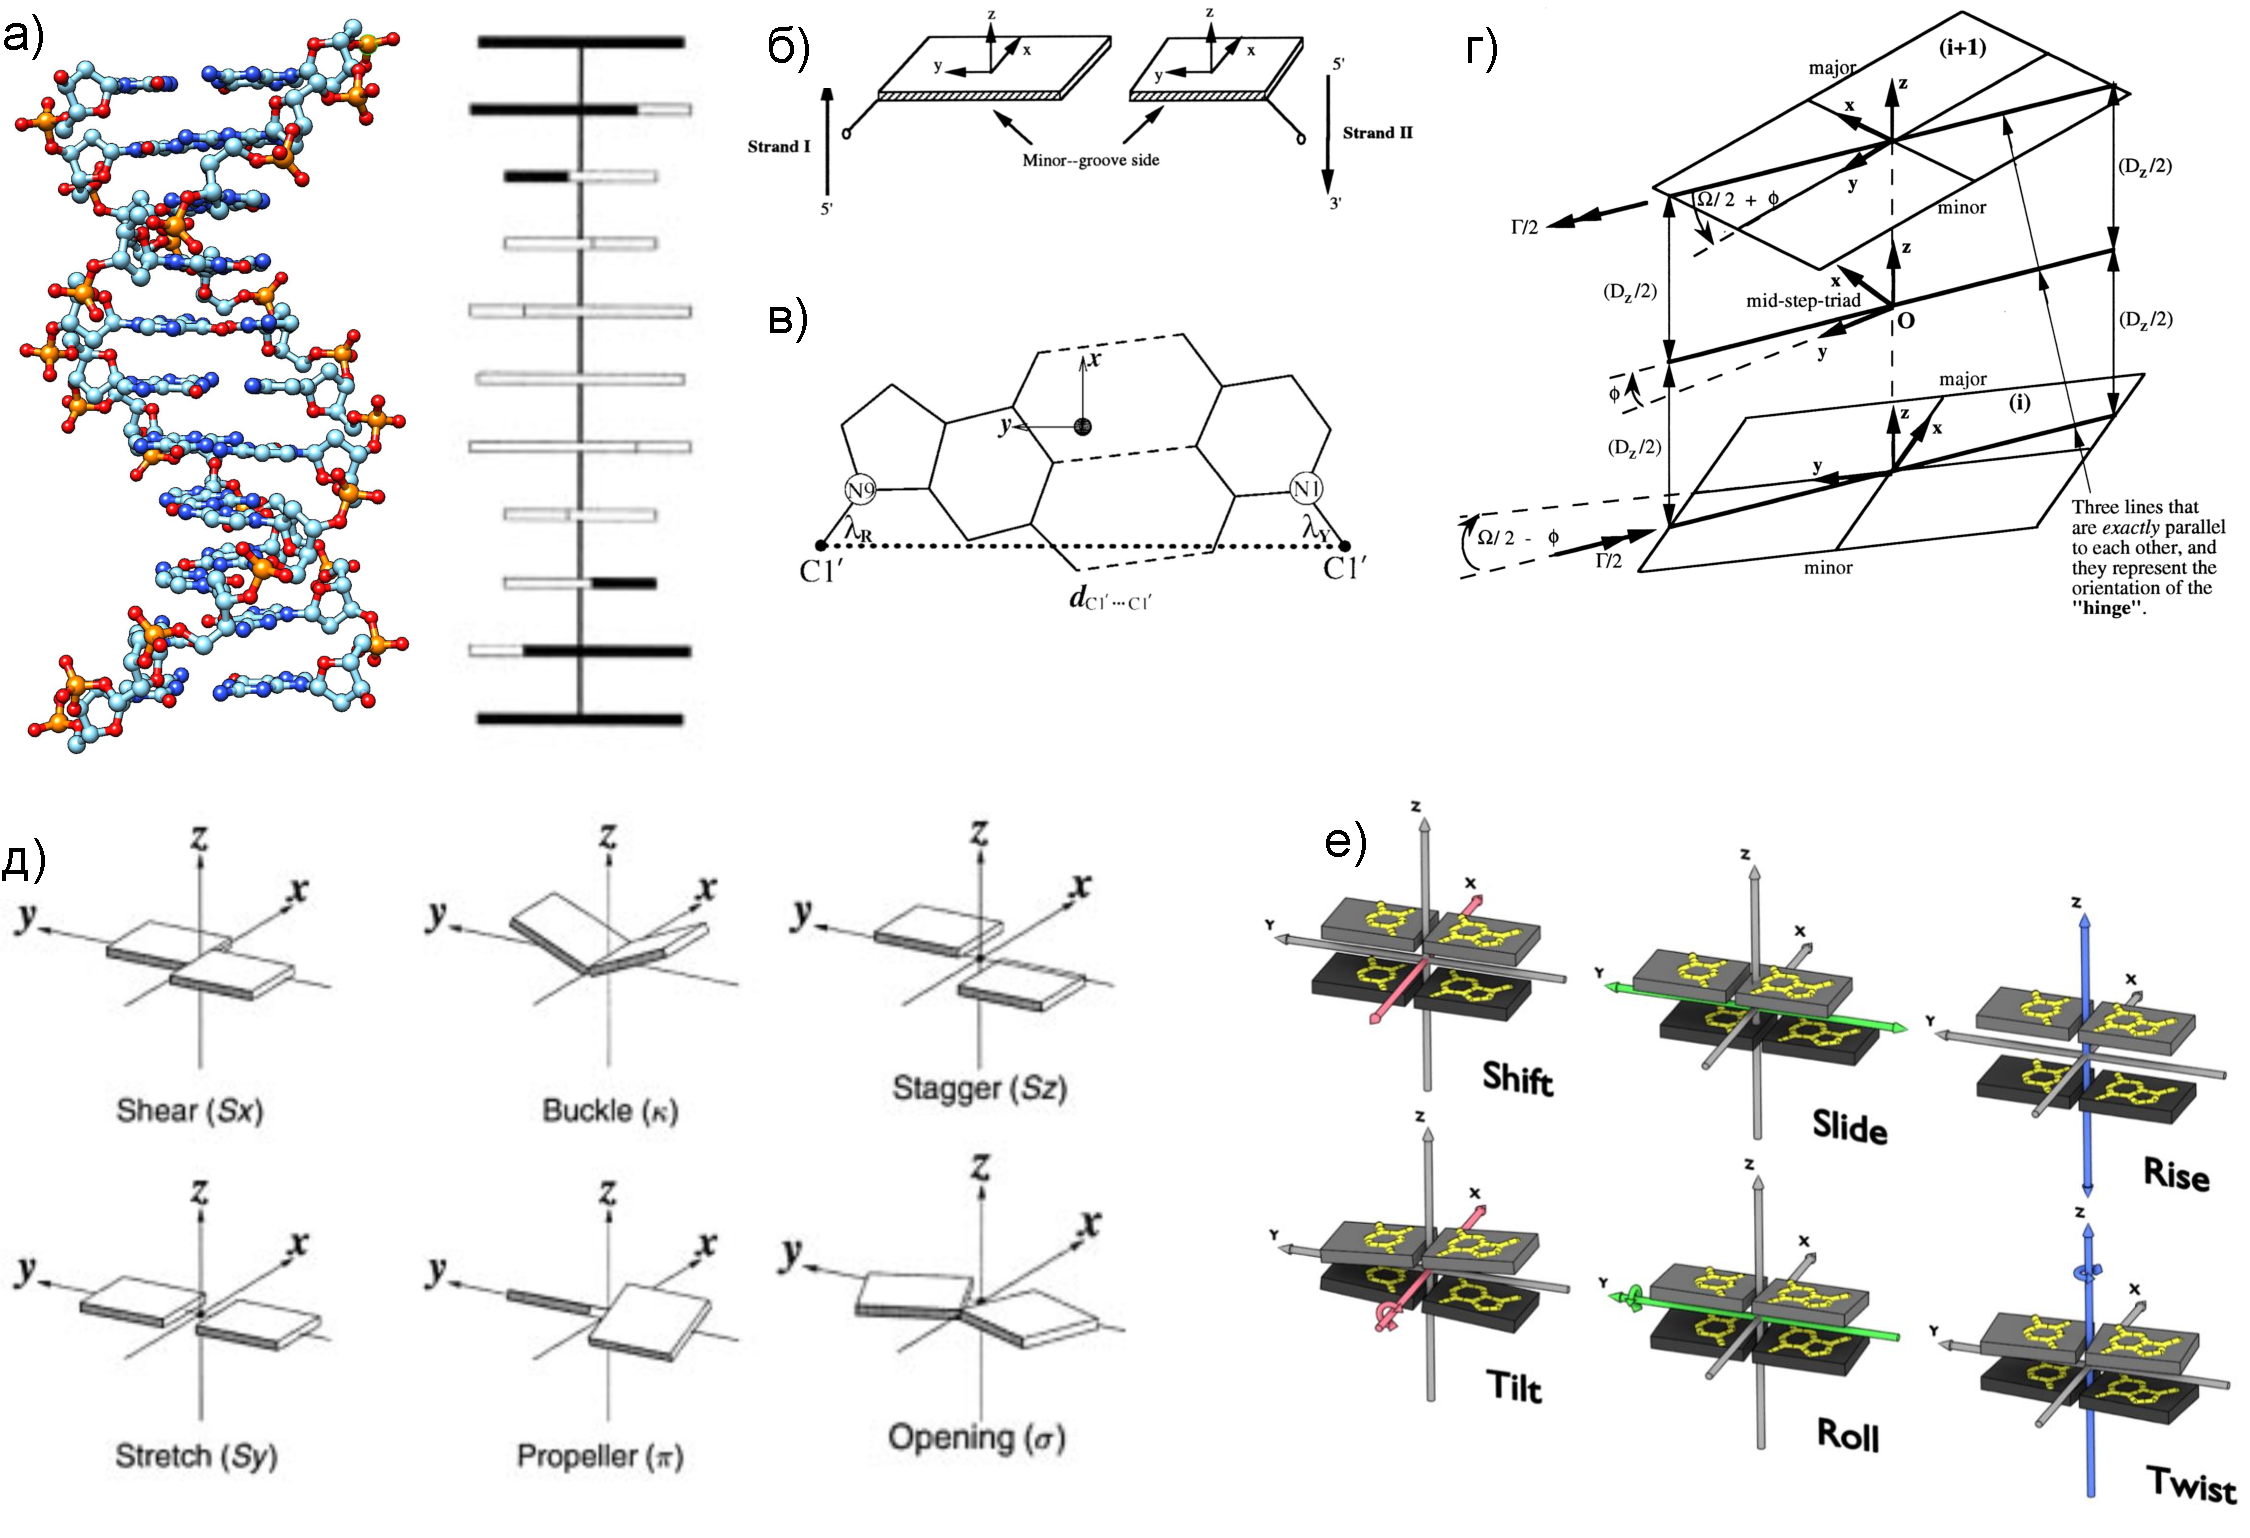
\includegraphics [width=\textwidth] {images/p1/DNA_param}
  \caption[Описание геометрии ДНК в виде геометрических параметров]{Описание геометрии ДНК в виде геометрических параметров. a) Атомистическое представление B-формы ДНК и представление в виде диаграммы по принципам Калладайна и Дрю \cite{calladine_understanding_2004}; б) представление пары оснований в виде параллелепипедов и связанные с ними системы координат \cite{el_hassan_assessment_1995}, в) система координат и ее расположение относительно пары оснований \cite{olson_standard_2001}, г) иллюстрация введения промежуточной системы отсчета между парами оснований для расчета параметров вращения  \cite{el_hassan_assessment_1995}, д) параметры взаимного расположения оснований в паре оснований \cite{lu_3dna_2003}, е) параметры взаимного расположения пар оснований относительно друг друга вдоль ДНК.} 
  \label{fig:p1:DNA_param}
\end{figure}

\subsection{Эмпирические константы жесткости изгиба ДНК}
Возможность задания общей конформации ДНК в виде набора 12 параметров, определяющих взаимное расположение азотистых оснований, позволяет поставить вопрос о возможности задания некоторого силового поля, способного описывать энергию различных конформаций двухцепочечной ДНК как функцию этих параметров. Для двухцепочечной ДНК любой последовательности, содержащей N пар оснований, 6(N-1) параметров будут описывать взаимное расположение пар оснований относительно друг друга. Формально с точки зрения статистической физики, поскольку каждой конкретной конформации ДНК однозначно можно сопоставить численные значения этих параметров и параметры являются независимыми, то набор этих параметров можно рассматривать как набор обобщенных координат (координат реакции), в пространстве которых может быть задана функция свободной энергии.

В общем случае данная функция будет иметь сложную структуру. Для того, чтобы такой формализм мог быть использован на практике, необходимо вводить ряд приближений относительно структуры данной функции. Наиболее используемым является, так называемое, динуклеотидное аддитивное приближение. Предполагается, что функция свободной энергии аддитивно складывается из компонент, описывающих вклады отдельных динуклеотидных шагов:

\begin{equation}
    F_{tot}(\{\theta^1_j\}, \{\theta^2_j\}, ... , \{\theta^{N-1}_j\})=\sum_{i=1}^{N-1}F_k(\{\theta^k_j\})
\end{equation}
где $k$ - номер динуклеотидного шага, $\{\theta^k_j\}$ - набор 6 переменных Roll, Tilt, Twist, Shift, Slide, Stagger для динуклеотидного шага $k$. 

Следующим упрощением является введение гармонического приближения для представления свободной энергии каждого динуклеотидного шага в виде разложения функции до второго порядка вблизи точки равновесия.
\begin{equation}
    F_k(\{\theta^k_j\})=F_0+\frac{1}{2}\sum_{i=1}^{6}\sum_{j=1}^{6}f_{ij}\Delta\theta^k_{i}\Delta\theta^k_{j}\\
    \Delta\theta^k_{i}=(\theta^k_{i}-\hat{\theta}^k_{i})
    \label{DNA_ener}
\end{equation}
Наконец, последним важным приближением является предположение о том, что коэффициенты $f_{ij}$ и равновесные значения $\hat{\theta}^k_{i}$ зависят только от типа конкретного динуклеотидного шага и не зависят от типа соседних нуклеотидов. Такое приближение называется приближением ближайших соседей (nearest neighbor). Следует отметить, что это лишь приближение, и в некоторых  особых случаях учета ближайших соседей не хватает для адекватного описания - например, когда важны коллективные эффекты вдоль по цепи, связанные с бифуркациями водородных связей, образованием цепочек воды в малой бороздке и т.д. Например, такие эффекты известны при рассмотрении протяженных участков аденина или тимина (А-траки), которые обладают высокой изгибной жесткостью.

Оценка констант $f_{ij}$ для каждого типа динуклеотидных шагов (всего их 10: CG,CA,TA,AG,GG,AA,GA,AT,AC,GC; в силу симметрии ДНК, напр. динуклеотидные шаги AA и TT обозначают один и тот же шаг, но по разным цепям) является нетривиальной задачей. На сегодняшний день существует два подхода - анализ кристаллических структур или расчеты методами молекулярного моделирования на основе атомистических силовых полей.

Первый подход был в значительной степени реализован в работе \cite{olson_dna_1998}. Авторами был проанализирован набор из 92 комплексов белок-ДНК и построены распределения динуклеотидных параметров в этих структурах (см. Рис. \ref{fig:p1:olson_DNA_param}). Предполагается, что изучая ансамбли распределений динуклеотидных параметров в комплексах ДНК-белок, можно получить информацию о подвижности и гибкости ДНК самой по себе. Аргументация данного предположения авторами сводится к следующему. Различные белки при связывании оказывают различные воздействия на  конформацию молекулы ДНК, таким образом, при достаточно большом усреднении и рассмотрении конформации ДНК вблизи равновесия в статистике будет проявляться лишь естественная склонность ДНК к деформациям.
Более строгим образом такое предположение обосновать сложно. Однако из анализа структур белков, известно, что распределение различных параметров полипептидной цепи в глобулярных белках обладает квази-больцмановской статистикой по отношению к энергетическим функциям, описывающим их локальные взаимодействия. Например, встречаемость различных ротамеров боковых цепей аминокислот согласуется с больцмановским распределением, описываемым функцией потенциальной энергии вращения вокруг соответствующей связи. Аналогичные наблюдения имеются для экспонированности боковых цепей аминокислот в воду и энергии их гидратации \cite{shaytan_solvent_2009}. Теоретическое объяснение этого явления было дано Финкельштейном и др. \cite{finkelstein_why_1995}. Описывая белок как гетерополимер согласно модели случайных энергий (Random Energy Model), можно показать, что количество аминокислотных последовательностей, которое стабилизируют тот или иной элемент белкового фолда, экспоненциально убывает с увеличением энергии этого элемента. Таким образом, квази-Больцмановская статистика является следствием устройства энергетического спектра нативных белков, у которых должна быть одна выраженная нативная конформация, энергетический уровень которой является самым низким по энергии и отделен энергетической щелью. Следуя этой логике, можно предположить, что количество различных белков, которые могут изгибать ДНК с той или иной силой, также будет экспоненциально зависеть от энергии изгиба ДНК.
\begin{figure}[H] 
  \center
  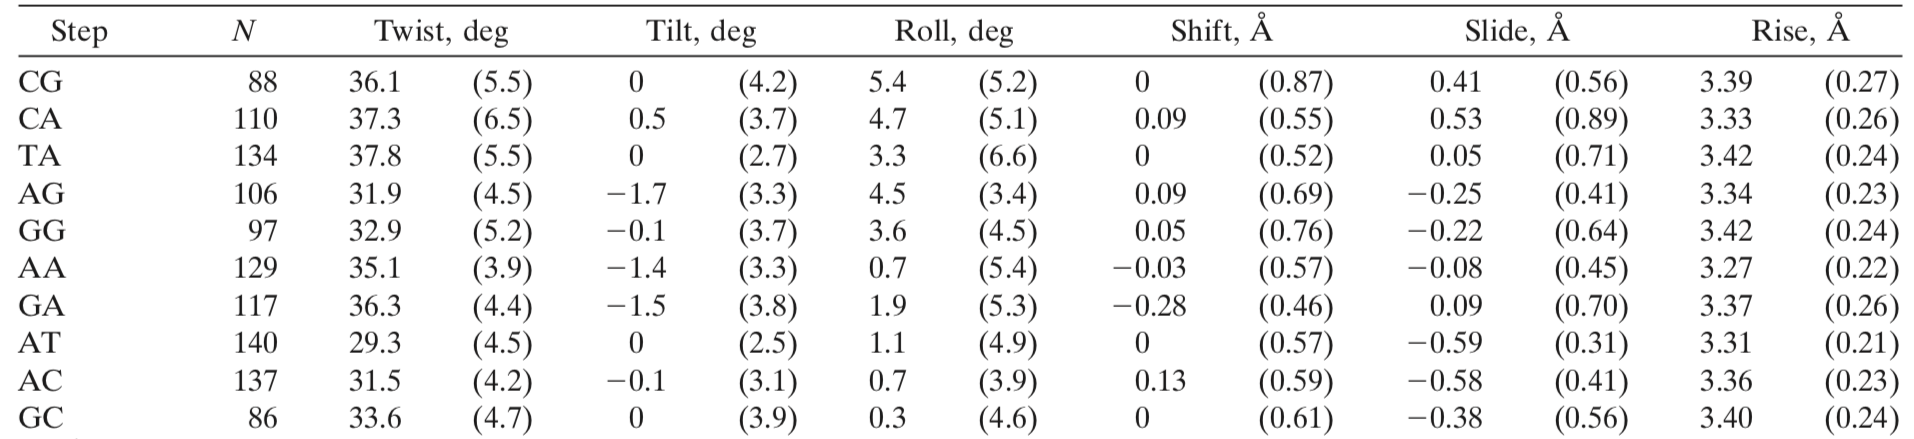
\includegraphics [width=\textwidth] {images/p1/olson_DNA_param}
  \caption{Матрица средних значений и отклонений динуклеотидных параметров из статьи \cite{olson_dna_1998}.} 
  \label{fig:p1:olson_DNA_param}
\end{figure}

Вычислив параметры отклонения ДНК в зависимости от типа динуклеотидного шага, а также дисперсии этих параметров, можно ставить задачу об оценке констант жесткости изгиба ДНК по этим различными параметрам $f_{ij}$ методом обратного гармонического анализа. В случае одномерной пружины, энергия которой описывается гармоническим законом $E=\frac{1}{2}fx^2$, распределение координаты согласно закону Больцмана будет выглядеть как $P(x) \sim \exp{-\frac{fx^2}{2kT}}$. Последнее является нормальным распределением с параметром дисперсии $\langle x^2 \rangle=kT/f$. Таким образом, мы установили связь дисперсии величины с константой жесткости.
В общем случае, когда энергия описывается функцией вида \ref{DNA_ener},  распределение состояний описывается многомерным нормальным распределением вида:
\begin{equation}
    P_{\mathbf X}(x_1,\ldots,x_k) = \frac{\exp\left(-\frac 1 2 ({\mathbf x}-{\boldsymbol\mu})^\mathrm{T}{\boldsymbol\Sigma}^{-1}({\mathbf x}-{\boldsymbol\mu})\right)}{\sqrt{(2\pi)^k|\boldsymbol\Sigma|}}
\end{equation}
где $|\boldsymbol\Sigma|=\det \boldsymbol\Sigma$, а $\boldsymbol\Sigma|$ - является матрицей ковариаций. Таким образом, несложно увидеть, что 
\begin{equation}
    \langle   \Delta\theta_{i} \Delta\theta_{j}\rangle=kT[{\boldsymbol F^{-1}}]_{ij}
\end{equation}
где ${\boldsymbol F}$ матрица коэффициентов $f_{ij}$, k - коэффициент Больцмана, $T$- конформационная температура, которую можно определить, например, сравнив получаемую гибкость с известными данными о персистентной длине. Константы жесткости доступны по адресу \url{https://web.archive.org/web/20151025043044/http://rutchem.rutgers.edu/~olson/pdna.html}.


Альтернативным подходом является вычисление характеристик динуклеотидных параметров путем молекулярного моделирования на основе атомистических силовых полей. Наиболее актуальной и современной здесь является работа \cite{walther_multi-modal_2020}. Авторы использовали наработки ABC консорциума, участники которого промоделировали методом атомистической молекулярной динамики все возможные последовательности тетрануклеотидов (всего их 136) \cite{dans_static_2019}. Из данных траекторий можно получить данные о флуктуациях различных параметров. Было показано, что распределения динуклеотидных параметров в некоторых случаях являются мультимодальными и их сложно аппроксимировать в виде одного многомерного гауссова распределения. Поэтому в данной статье некоторые распределения параметров описываются линейной комбинацией многомерных гауссовых распределений. Кроме того авторы делают попытку сделать коэффициенты $f_{ij}$ зависимыми от соседних с динуклеотидным шагом пар оснований - эффективно учитывая параметры изгибной жесткости ДНК на тетрануклеотидном уровне.

Суммируя вышесказанное, отметим достоинства и недостатки различных подходов. Гармоническое приближение при описании гибкости ДНК безусловно имеет свои ограничения, особенно в случаях, когда белок сильно деформирует ДНК. Например, в нуклеосомах динуклеотиды  пиримидин-пурин (YR) обычно выгибаются в сторону малой бороздки (параметр Roll отрицательный), в то же время из Рис. \ref{fig:p1:olson_DNA_param} видно, что в среднем в структурах динуклеотиды имеют положительный Roll, причем, динуклеотид TA (YR) больше склонен к положительному Roll, чем AT (RY). Однако предполагается, что при сильных изгибах (изломах, kinks) поверхность энергии устроена более сложным образом, и при комбинации с положительными значениями Slide - как раз AT выгоднее гнуться в сторону малой бороздки, чем TA \cite{wang_sequence-dependent_2010}. В этом плане мультимодальное приближение изгибной жесткости ДНК может являться более точным. Однако, для мультимодального приближения требуется большое количество качественных данных о динамике ДНК, которые, казалось бы, можно взять из молекулярно-динамических расчетов. Однако, здесь есть свой подводный камень - атомистические силовые поля, существующие на сегодняшний день, не совсем корректно описывают зависимость изгибной жесткости ДНК от последовательности в сравнении со структурными данными. Так, например, по данным вычислений молекулярной динамики максимальным значением параметра Roll Roll обладает динуклеотид TG \cite{pasi_muabc_2014}, а по данным анализа кристаллических структур CG.

\subsection{Программные продукты}
Для анализа геометрии ДНК был создан достаточно большое набор программных продуктов и методов, к ним можно отнести программы CompDNA\cite{gorin_b-dna_1995}, SCHNAaP \cite{lu_structure_1997}, Curves+ \cite{lavery_conformational_2009}, 3DNA \cite{lu_3dna_2008}. На данный момент наиболее используемой и поддерживаемой является программа 3DNA, которая позволяет не только анализировать структуру, но и реконструировать атомистическую структуру по набору параметров. Для анализа ширин и глубин бороздок ДНК может использовать программа Curves+.
Моделирование конформации ДНК в динуклеотидном приближении сводится к реализации либо алгоритмов минимизации конформации ДНК в пространстве параметров, либо к динамическим расчетам с помощью метода Монте-Карло. Многие такие программы разрабатывались для решения конкретных научных задач внутри научных групп, например, DNAminiCarlo (N.B. Ulyanov,
A.A. Gorin, V.B. Zhurkin), аналогичные подходы описаны в ряде статей \cite{norouzi_topological_2015,kulaeva_internucleosomal_2012}, недавно появилась программа MC-enNN и веб-сервер к ней \cite{walther_multi-modal_2020}. В нашей научной группе проводится разработка программы с открытым программным кодом PyNAMod
 \url{http://github.com/intbio/PyNAMod}, способной моделировать ДНК, включая ДНК-белковые комплексы в динуклеотидном приближении методами минимизации геометрии ДНК, а также методом цепей Монте-Карло.

\subsection{Алгоритмы интегративного моделирования}
\label{sec:p1:int_algo}
Введение дополнительных ограничений при моделировании ДНК в динуклеотидном приближении, а также учет стерических ограничений путем конвертации структуры из пространства динуклеотидных параметров в атомистическую структуру, позволяют сформулировать подходы для интегративного моделирования ДНК и комплексов-ДНК белок на основе различных экспериментальных данных.

В реализованных нами подходах при минимизации конформации ДНК в динуклеотидном приближении в энергию системы вводились дополнительные члены, соответствующее отклонению набора расстояний от целевых значений, измеренных при помощи экспериментальных методов, например, spFRET. Алгоритм действия программы изображен на Рис. \ref{fig:p1:int_mod_dinuc}. На вход программа получает начальные структуры в формате PDB. Измерения методом spFRET дают информацию о расстояниях между парами меток. Алгоритм последовательно оптимизирует координаты нуклеотидных пар таким образом, чтобы привести их геометрию в соответствие с результатами spFRET. В ходе работы алгоритма учитываются ограничения, связанные с жесткостью ДНК.


\begin{figure}[H] 
  \center
  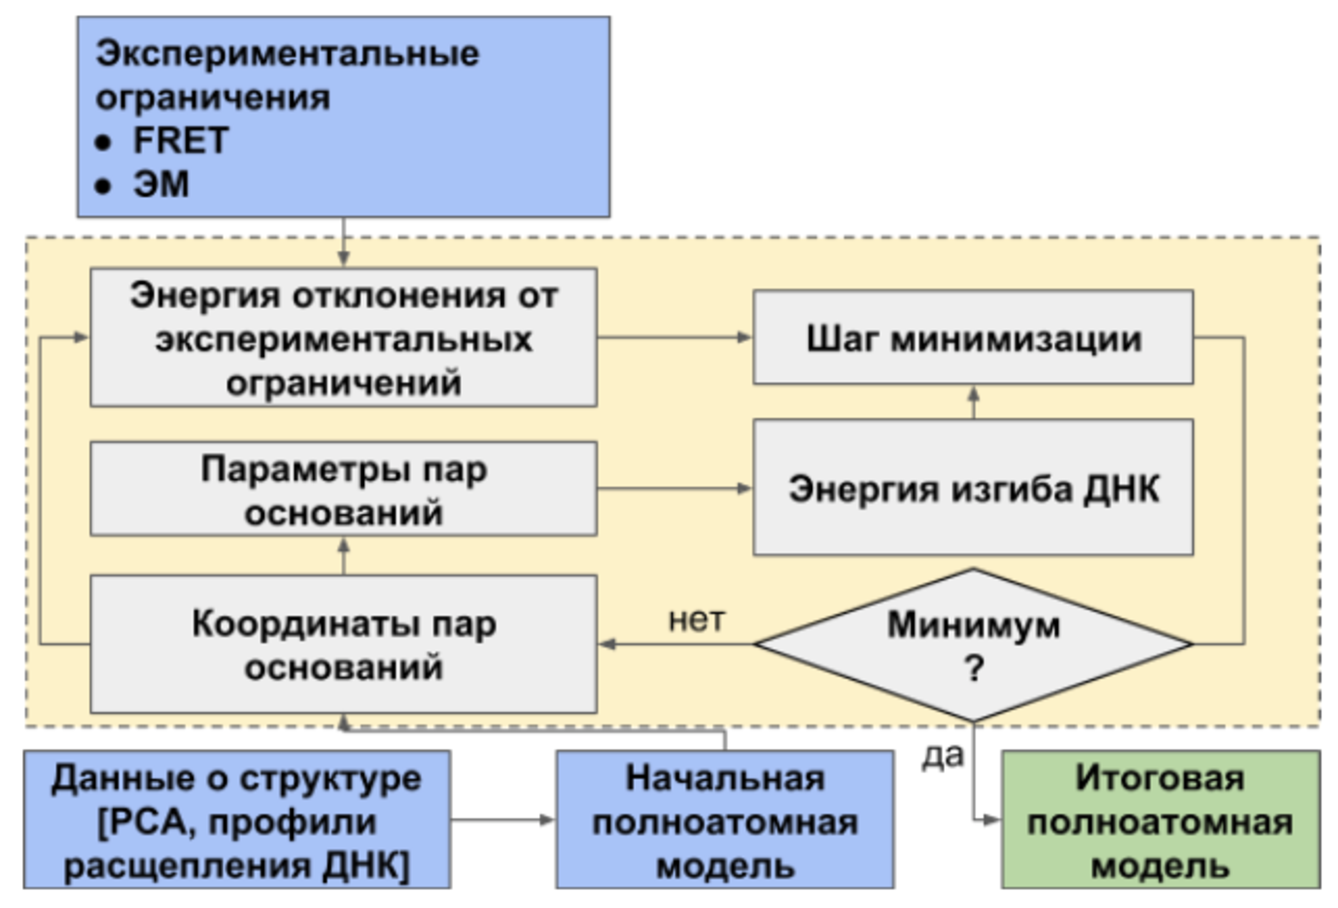
\includegraphics [width=\textwidth] {images/p1/int_mod_dinuc}
  \caption{Алгоритм интегративного моделирования на основе моделей ДНК в динуклеотидном приближении.} 
  \label{fig:p1:int_mod_dinuc}
\end{figure}
%\section{Методы моделирования супрануклеосомной структуры хроматина}
\section{Методы моделирования супрануклеосомной структуры хроматина}
% сделать на основе https://docs.google.com/document/d/1A_RRCcKiU5YPzdSMHhqiwX-g2PkqbeQ4iB5KrB0_MFI/edit?usp=sharing

    В последние годы благодаря совершенствованию экспериментальных технологий наметилась долгожданная конвергенция методов структурной биологии и методов геномики в изучении организации хроматина на молекулярном уровне. Благодаря успехам крио-электронной микроскопии, мы получаем все больше информации о структуре не только нуклеосом, но и супрануклеосомных структур, а благодаря развитию методов геномики и 3-D геномики все более высокого разрешения, стало возможным определять контакты между локусами ДНК с суб-нуклеосомным разрешением (в частности, методы Micro-C, Micro-C-XL и др.) и определять положение и состав нуклеосом вдоль генома (напр. методы MNase-seq, MNase-ChIP-seq). Возникает необходимость в интерпретации экспериментальных данных и построении физических молекулярных моделей укладки хроматина на супрануклеосомном уровне с учетом реальных геометрических и топологических параметров молекул белков и ДНК, а также динамического характера этих взаимодействий.

    Так как изучение организации хроматина на супрануклеосомном уровне довольно давно представляет собой фундаментальную задачу для молекулярной и клеточной биологии (примем за дату начала год открытия нуклеосомы и структуры в виде ``бусин на нити'' - 1974 \cite{kornberg_chromatin_1974}), было разработано множество подходов к молекулярному моделированию укладки нуклеофиламента. Большую часть прошедшего времени сомнений в концепции 30-нанометровой фибриллы не возникало (идею 30-нанометровой фибриллы предложили в 1980 году, серьезные аргументы против появились в 2000-ых, 2010-ых  см., например, \cite{joti_chromosomes_2012,razin_chromatin_2014}). Поэтому подавляющее число работ по молекулярному моделированию хроматина на супрануклеосомном уровне являются по сути работами по моделированию 30-нанометровой фибриллы, что, не умаляя их методологической значимости, значительно снижает ценность результатов и приводит к необходимости проведения работ по молекулярному моделированию хроматина на супрануклеосомном уровне с учетом современных знаний о нем.  При этом изучение предыдущей литературы по данной теме все-таки необходимо, так как ее авторы достигли значительных результатов в разработке математического и концептуального  аппарата для моделирования хроматина на этом уровне вообще. Например, в работе 2015 года Norouzi, D. \& Zhurkin, V. B. Topological Polymorphism of the Two-Start Chromatin Fiber \cite{norouzi_topological_2015} авторы с помощью своей модели изучили все возможности организации двухстартовой хроматиновой фибриллы (есть два гипотетических типа организации 30-нанометровой хроматиновой фибриллы: соленоидная - одностартовая фибрилла - и зигзагом - двухстартовая фибрилла - причем тип фибриллы коррелирует с длиной ликерного участка), т.е. смоделировали все возможные ее конформационные варианты. Фибриллы моделировали симметричными и регулярными, а для расчетов вводилось 4 параметра суперспирализации: кручение, подъем, наклон нуклеосом и диаметр. Энергия фибриллы задавалась как сумма четырех слагаемых: эластической энергии линкерной ДНК, стерического отталкивания, электростатики (рассчитываемой с помощью кулоновского потенциала), феноменологического взаимодействия между двумя ``сложенными в стопку'' нуклеосомами. При оптимизации энергии фибриллы с учетом параметров суперспирализации исследователи впервые обнаружили два типа топологического перехода в ней: путем резкого на 360 градусов поворота в кручении линкера и путем скрещивания линкеров. Даже при моделировании структуры, отличной от 30-нанометровой фибриллы, эти принципы могут быть релевантными, так как позволяют рассчитать такие общие вещи, как энергию комплекса ДНК-нуклеосома, его оптимальную геометрию в зависимости от длины линкеров и внешних факторов. Эти же авторы  в более поздней  работе того же года продолжали исследовать топологический полиморфизм хроматиновой фибриллы, пытаясь установить связь между длиной линкеров и спецификой сверхспирализации ДНК (связанной с уровнем транскрипции). Интересно, что для нахождения оптимальной конформации линкерной ДНК использовался мезоскопический подход: ДНК моделируется динуклеотидными ``шагами'', его траектория описывается с помощью шести параметров: Tilt, Roll, Twist, Shift, Slide, Rise. Мезоскопический подход был  предложен в статье Olson et al., 1993 \cite{olson_influence_1993}, данные шестимерные координаты - в работе Dickerson et al., 1989 \cite{dickerson_definitions_1989}. Оба этих концептуальных инструмента широко используются в моделировании хроматина на низких уровнях компактизации (10-нанометровой фибриллы и следующем) и никак не зависят от концепции 30-нанометровой фибриллы, что делает их полезными и для моделирования альтернативных этой фибрилле структур. Крайне эффективным для молекулярного моделирования супрануклеосомного уровня компактизации хроматина являются методы, основанные на принципах Монте-Карло. Познакомиться с ними можно, например, в работе — Norouzi, D. \& Zhurkin, V. B. Dynamics of Chromatin Fibers: Comparison of Monte Carlo Simulations with Force Spectroscopy \cite{norouzi_dynamics_2018}. Шаги симуляции следующие: случайный выбор одной пары оснований в подвижном линкере и изменение его шести параметров, обновление позиций нуклеосом в нуклеосомном массиве, вычисление разницы в энергии между старым и новым состоянием и выполнение теста Метрополиса. Варьируя величину внешних сил, степень развернутости (unwrapping) нуклеосом, длину нуклеосомных повторов (NRL - nucleosome repeat length) - среднее расстояние между центрами соседних нуклеосом и значение энергии стэкинга (stacking energy), исследователи провели серию симуляций, каждая из которых включала около 100 миллионов описанных выше шагов. Подобный подход, особенно его вариант - моделирование путем имитации отжига - позволяет довольно эффективно находить глобальный энергетический минимум в заданной системе.
    
    Также часто применяется для решения задач моделирования хроматина на разных уровнях организации метод огрубленного моделирования (coarse-grained). Суть метода состоит в представлении молекул и молекулярных структур (например, нуклеосом) простыми телами и поверхностями: сферами, цилиндрами, плоскостями. Такое приближение значительно упрощает вычисления и позволяет проводить однозначный анализ за приемлемое время. Однако при этом исходные данные подвергаются соответствующей деформации - результат моделирования соответствует им не полностью, он также зависит от выбранной стратегии огрубления. Хроматиновые фибриллы и их динамику обычно моделируют как цепочки из шаров или как червеобразные структуры \cite{korolev_systematic_2018,savelyev_molecular_2009,ozer_chromatin_2015}. Несмотря на популярность метода огрубленного моделирования в области изучения структуры хроматина, он является далеко не оптимальным для решения этих задач: исходные данные не используются полностью, искажаются, что может быть критичным, когда речь заходит об изучении укладки 10-нанометровой фибриллы, так как образуемая ею структура зависит от не учитываемых в огрубленных методах параметров - например, длины линкера \cite{norouzi_topological_2015,nikitina_dna_2017,norouzi_topological_2015}. Для адекватного моделирования структуры хроматина требуется основывать его на данных высокого разрешения (например, современных протоколов Hi-C), причем они не должны искажаться так сильно, как в методе огрубленного моделирования. Таким образом необходимо разработать новый, более чувствительный к данным и параметрам наподобие длины линкеров подход. 

    Важно отметить, что большинство описываемых выше подходов основаны на ``закрытом'' программном обеспечении. Авторы либо не предоставляют доступа к программному обеспечению, либо оно является слабо используемым, поскольку к нему нет описания, либо возникают проблемы с переносимостью.

\begin{figure} [h!]
    \centering
    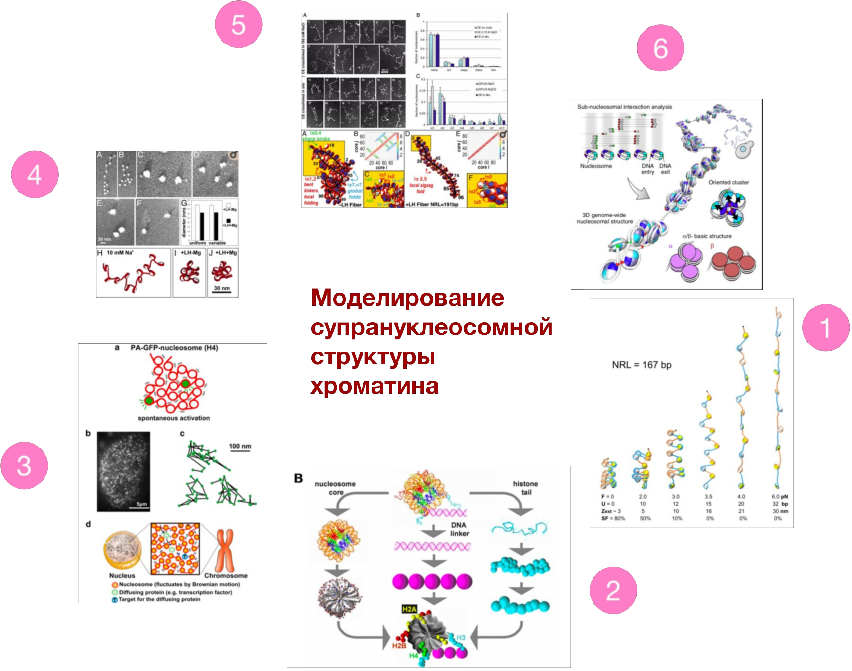
\includegraphics [width=\textwidth]{images/p1/part1_4_cm/part1_4_cm_f6.pdf}
    \caption[Подходы к моделированию супрануклеосомной структуры]{Подходы к моделированию супрануклеосомной структуры, в том числе с учетом экспериментальных данных. (1) - Молекулярная динамика с использованием принципов Монте-Карло \cite{norouzi_dynamics_2018}; (2) - Огрубленное моделирование \cite{schlick_monte_2009}; (3) - (6) : интегративные методы. (3) - Моделирование на основе данных метода Single nucleosome imaging  - отображения одиночных нуклеосом \cite{maeshima_chromatin_2014}; (4), (5) - Моделирование на основе данных метода EMANIC - метода обнаружения нуклеосом с помощью электронной микроскопии \cite{grigoryev_evidence_2009}, \cite{grigoryev_hierarchical_2016}); (6) - Моделирование супрануклеосомной структуры на основе данных модифицированного Micro-C   \cite{ohno_sub-nucleosomal_2019}}.
    \label{fig:p1_4:f6}
\end{figure}


    Важным подходом является интеграции различных экспериментальных данных при построении моделей - данный подход называется интегративным моделированием. В применении к супрануклеосомной структуре он на наш взгляд развит весьма слабо. На данный момент по данным литературы известна лишь одна попытка интеграции данных Micro-C с методами моделирования. Работа опубликована в 2019 году \cite{ohno_sub-nucleosomal_2019}. В ней приведены довольно убедительные доказательства существования определенных супрануклеосомных структур в геноме пекарских дрожжей, альтернативных отвергнутой  хроматиновой фибрилле, - хроматиновых альфа-тетраэдров и бета-ромбов - то есть этой работой был сделан большой шаг на пути к определению структуры хроматина на до сих пор не исследованных уровнях компактизации генома. Молекулярное моделирование проводилось на основании теоретической модели нуклеосомы - как комплекса из гистонового октамера и ассоциированной с ним ДНК — и данных Micro-C, позволяющих различать точки ``входа'' и ``выхода'' ДНК в/из нуклеосом. Такой комбинированный метод был назван Hi-Co. Само моделирование проводилось с помощью подхода имитации отжига в методе молекулярной динамики. Имитация отжига была необходима для оптимизации позиций и ориентаций отдельных нуклеосом, остальные структурные факторы, такие как, например,  линкерная ДНК (ее длина), были неявно включены в потенциалы и по сути не рассматривались детально. Несмотря на важное значение, подходы моделирования в работе Ohno et al.  не вполне реалистичны, так как, например,  отсутствуют в явном виде линкерная ДНК, а следовательно не учитывается влияние топологии и кручения ДНК важные для понимания многих функциональных процессов и состояний в хроматине. Также в подходе авторов не предполагался учет нуклеосом различного типа и возможного откручивания ДНК от нуклеосомы с изменением углов входа/выхода ДНК. Кроме того работа Ohno et al. была посвящена изучению генома дрожжей — это значит, что непосредственной значимостью для медицины она не обладает. Требуется провести аналогичное исследование генома высших, многоклеточных эукариот и человека.

%картинка
\begin{figure} [h!]
    \centering
    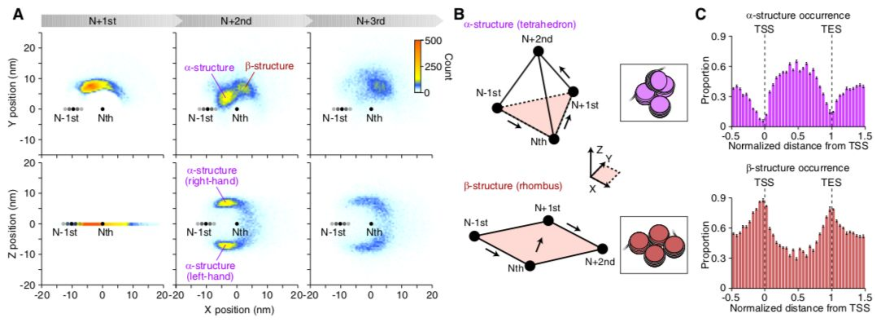
\includegraphics[width=\textwidth]{images/p1/part1_4_cm/part1_4_cm_f7.pdf}
    \caption[Визуализация анализа данные Micro-C, Ohno et al., 2019]{Визуализация результатов анализа взаимного расположения нуклеосом в пространстве и выявленные в результате него мотивы супрануклеосомной структуры ДНК из статьи Ohno et. al, 2019}
    \label{fig:p1_4:f7}
\end{figure}

Для моделирования супрануклеосомной укладки фибрилл алгоритмы, предложенные нами в пункте \ref{sec:p1:int_algo}, могут быть адаптированы путем включения дополнительных данных из экспериментов Micro-C, а также данных о позициях нуклеосом из экспериментов MNase-seq, ATAC-seq (см. Рис. \ref{fig:p1_4:f8}). 
     Расчет обобщенных переменных из атомистической структуры и восстановление координат из набора переменных, описывающих геометрию ДНК в динуклеотидном приближении, производится при помощи программы 3DNA \cite{lu_3dna_2003}, либо при помощи разрабатываемой программной библиотеки PyNAMod.      Учет положения и геометрии белковых компонент можно производить в том же приближении: для этого необходимо определять их ориентацию относительно ключевых динуклеотидов. Например, при определении гистонового ядра нуклеосомы, отсчитывать его положение относительно диадного динуклеотида.
    Дополнительно в физическую модель нуклеосомной фибриллы вводятся парные потенциалы для учета исключенного объема и электростатических взаимодействий между соседними нуклеосомами, что необходимо для учета изменяющих заряд посттрансляционных модификаций гистоновых хвостов.
     При моделировании цепочек нуклеосом, вводятся ограничения на расстояния, описывающие межнуклеосомные контакты. Возможно также введение дополнительного потенциала, позволяющего нуклеосомам смещаться относительно их изначальных положений (что обосновано точностью определения их положения в эксперименте).   В рамках описываемой физической модели нуклеосомной фибриллы можно создавать модели организации хроматина путем применения численных методов минимизации значений функции, например метода градиентного спуска, однако, для обнаружения глобального минимума, а также создания множественной выборки из конфигурационного пространства более применимы стохастические подходы, такие как метод  Монте-Карло с алгоритмом Метрополиса.

\begin{figure} [h!]
    \centering
    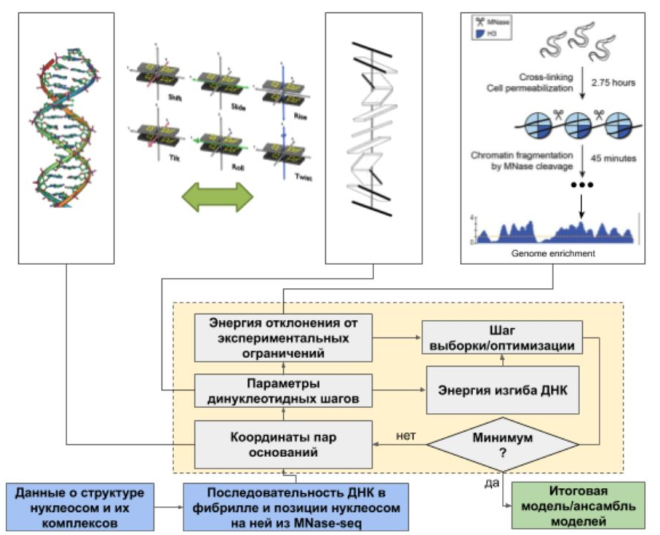
\includegraphics [width=\textwidth]{images/p1/part1_4_cm/part1_4_cm_f8.pdf}
    \caption[Алгоритмы интегративного моделирования нуклеосомных фибрилл]{Алгоритмы интегративного моделирования нуклеосомных фибрилл. Слева вверху - схематическое описание ДНК в приближении динуклеотидных шагов. Справа вверху - сокращенное схематическое представление методов Micro-C/MNase-seq/MNase-ChIP-seq. Снизу - Описание подхода интеграции экспериментальных данных в физическую модель нуклеосомных фибрилл.}
    \label{fig:p1_4:f8}
\end{figure}











\section{Основы некоторых экспериментальных методов}
%\subsection{Футпринтинг ДНК с использованием гидроксил-радикалов}
\subsection{Методы футпринтинга ДНК}
Одним из подходов к изучению структуры ДНК и ДНК-белковых комплексов являются методы физического, химического или ферментативного футпринтинга (от англ. footprint - след). Идея методов состоит в обработке ДНК определенными агентами, которые вносят изменения в ее химическую структуру в зависимости от ее конформации, состава или взаимодействия с другими макромолекулами, с последующим анализом продуктов реакции для установления мест химических реакций вдоль ДНК.

К физическим методам относят облучение ДНК ультрафиолетом \cite{becker_ultraviolet_1988} или рентгеном, что приводит к разрыву ДНК в областях не защищенных белком. С помощью секвенирующего гель электрофореза можно определить длины продуктов реакций и следовательно участки взаимодействия с белком. Аналогичный подход может быть осуществлен с использованием генерируемых в реакционной смеси гидроксил радикалов химическими методами. Методам гидроксильного футпринтинга посвящена глава \ref{part5_hrf} данной диссертационной работы. Наиболее популярным методом ферментативного футпринтинга является использование фермента ДНКазы I, обладающего выраженной эндонуклеазной активностью. К плюсам такого подхода относится простота осуществления эксперимента, к минусам большой размер фермента (около 4 нм), что уменьшает детальность футпринтинга, и наличие некоторой специфичности по последовательности (гидролизует ДНК преимущественно около пиримидинов). Еще одним интересным методом химического футпринтинга является футпринтинг с использованием перманганата калия. Перманганат калия связывается с тиминами в одноцепочечной ДНК, окисляет их, что приводит в конченом итоге к разрыву в ДНК. Таким образом можно исследовать локализацию пузырей транскрипции в геноме, нестандартных ДНК структур  \cite{kouzine_permanganates1_2017}. Футпринтинг с использованием диметилсульфата (ДМС) используется также для изучения ДНК-белковых взаимодействий. ДМС индуцирует метилирование остатков гуанина. Два образца обрабатывают пиперидином, чтобы вызвать химическое расщепление остатков гуанина, модифицированного ДМС, с последующим расщеплением рестрикционными ферментами. После маркировки образцы запускают параллельно на геле для визуализации. Отсутствующие полосы в образце, связанном с белком, соответствуют остаткам гуанина, защищенным от модификации посредством взаимодействия \cite{hornstra_vivo_1993}.

%\subsection{ФРЕТ спектроскопия и микроскопия}
\subsection{FRET спектроскопия и микроскопия}
%\todo{2S Из файла Armeev\_disser.pdf - со стр. 23 весь п. 1.4 с картинками. НО - нужно весь текст переписать так, чтобы его не детектировал антиплагиат - нужно чтобы подряд не было 3 похожих слов (!) можно перефоразировать, заменять на синонимы, менять местами слова}
%то есть до страницы 36 включительно?


\subsubsection{Ферстеровский резонансный перенос энергии}

    Ферстеровский резонансный перенос энергии (Forster resonance energy transfer, FRET) это эффект безызлучательного переноса энергии с одного красителя-флуорофора на другой. Пару (или более) флуорофоров подбирают таким образом, чтобы спектр поглощения акцептора перекрывался со спектром флуоресценции донора. Флуорофоры могут быть пришиты к аминокислотам или азотистым основаниям ДНК с помощью различных линкерных молекул. По определение эффективность FRET - это отношение вероятности переноса энергии с донора на акцептор по отношению ко всем другим переходам в расчете на событие возбуждение донора:
\begin{equation}
    E_{FRET} = \frac{k_\text{ET}}{k_f + k_\text{ET} + \sum{k_i}}
\end{equation}    
 где $k_{ET}$ - скорость переноса энергии с донора на акцептор, $k_f$ - скорость процесса флуоресценции донора,  $k_i$ - скорости других неизлучательных процессов релаксации донора, за исключением переноса энергии на акцептор.
    Эффективность переноса энергии существенно зависит от расстояния между метками и может быть описана следующей формулой:

\begin{equation}
    E_{FRET}=\frac{1}{1+(R/R_0)^6}
    \label{fret_E}
\end{equation}
    где R - расстояние между метками, $R_0$ - радиус
     Ферстера, расстояние между метками, отвечающее 50\% эффективности переноса энергии между флуорофорами (см. Рис. \ref{fig:p1_5_fret:f3}). Согласно данной формуле, измеряя эффективность FRET возможно вычислить расстояние между участками меченой макромолекулы. Для каждой пары меток радиус Ферстера индивидуален, он зависит от ряда факторов, в том числе от квантового выхода флуоресценции донора, ориентации красителя на поверхности молекулы (ориентационный фактор), коэффициента преломления среды и т.д. 

\begin{figure} [h!]
    \centering
    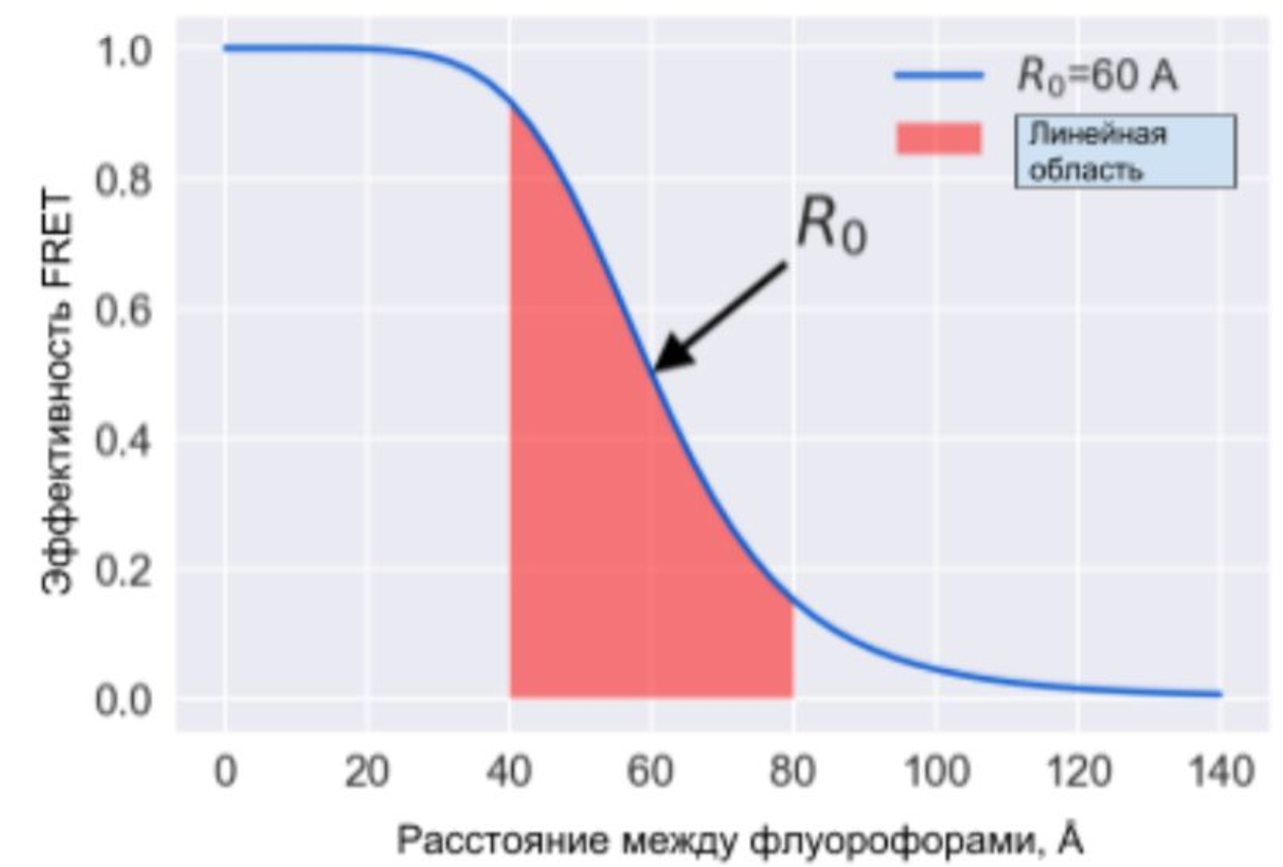
\includegraphics[width=\textwidth]{images/p1/part1_5_fret/part1_5_fret_f3.pdf}
    \caption[Зависимость эффективности переноса энергии от расстояния между флуорофорами.]{Зависимость эффективности переноса энергии от расстояния. Стрелкой показана величина Ферстеровского радиуса. Красным показана область изменений, близкая к линейной. }
    \label{fig:p1_5_fret:f3}
\end{figure}

    Эффективность переноса энергии может быть выражена через отношение времен жизни флуоресценции донора в отсутствии и присутствии акцептора:
\begin{equation}
    E_{FRET}= 1-\tau_{D}^{'}/\tau_D
\end{equation}
    где $\tau_{D}^{'}$ - время жизни флуоресценции донора в присутствии акцептора,  $\tau_D$ время жизни донора в отсутствии акцептора.
    
    Альтернативным является выражение эффективности переноса через величины интенсивности флуоресценции донора и акцептора:
    
\begin{equation}
   E_{FRET}=\frac{F_A}{F_A+\gamma F_D}
   \label{eq:p1:fret}
\end{equation}
    где $F_A= I_A - B_A - \alpha_{DA} (I_D - B_D) - D_{ex}$, $F_D = I_D - B_D - \alpha_{AD} (I_A - B_A )$ и 
В последних формулах $I_A$ и $I_D$  - регистрируемые интенсивности сигнала акцептора и донора, соответственно; $B_A$ и $ B_D$ - уровни фонового сигнала в канале акцептора и донора, соответственно;  $\alpha_{DA}$ и $\alpha_{AD}$ - перекрестные коэффициенты (crosstalk coefficients), характеризующие долю флуоресценции донора, регистрируемую в канале акцептора ( $\alpha_{DA}$ ), и долю излучения акцептора, регистрируемую в канале донора ( $\alpha_{AD}$ ). Поправочные коэффициенты помогают учитывать особенности  оптической схемы конфокального микроскопа или спектрофлуориметра, для разных пар флуоресцентных меток они отличаются. $D_{ex}$ - это величина сигнала прямого возбуждения акцептора (возникающая в следствие возможного поглощения фотонов акцептором на длине волны поглощения донора). $\gamma$ - так называемый фактор детекции, он позволяет учитывать различия в эффективностях детекции флуоресценции $(\eta)$ донора и акцептора и различия в их квантовых выходах флуоресценции ($\Phi$) \cite{dahan_ratiometric_1999}. Фактор детекции может быть представлен в виде:

\begin{equation}
    \gamma = \gamma_{instrument} \gamma_{dye} = \frac{\eta_A \Phi_A}{\eta_D \Phi_D}
\end{equation}
где $\Phi$ - квантовый выход, $\eta$ - эффективность детекции.
    Эффективность детекции флуоресценции зависит от спектральной чувствительности детекторов (лавинных фотодиодов или фотоэлектронных умножителей) и спектральных характеристик оптических элементов, через которые проходит сигнал от образца. 
    Измерение фактора детекции в ряде случаев может быть затруднено и его принимают за единицу. В таком случае измеряемая по формуле (\ref{eq:p1:fret}) величина является не истинным коэффициентом переноса, такую величину называют ``коэффициентом близости'' (PR - proximity ratio). Коэффициент близости нельзя непосредственно связать с расстоянием между флуоресцентными метками, однако, используя этот коэффициент можно делать выводы о гетерогенности образца, и о качественных эффектах сближения или удаления частиц.

\subsubsection{Детекция сигнала от одиночных молекул}
    Эффективность FRET может быть измерена в объеме сразу от многих частиц при помощи прибора спектрофлуориметра. В этом случае измеренный сигнал соответствует некоторому среднему сигналу от ансамбля молекул \cite{klose_simulation_2012}. Такой усредненный сигнал может не соответствовать ни одному конкретному состоянию системы на молекулярном уровне, а являться суперпозицией нескольких состояний разных частиц. Чтобы добиться связи сигнала FRET с конкретными состояниями молекулярной системы, необходимо, как минимум, измерять эффективности FRET у одиночных частиц, такой метод называется spFRET (single particle FRET). С помощью метода spFRET возможно оценивать как средние расстояния \cite{okumus_vesicle_2004}, так и временную динамику изменения расстояний между метками \cite{li_rapid_2005}. Вопрос заключается в том, каким образом снимать сигнал от одной частицы. Одни вариант заключается в иммобилизации частиц на поверхности. Иммобилизовав частицы, можно использовать подходы, основанные на эффекте полного внутреннего отражения, которые позволяют проводить измерения в тонком слое частиц у поверхности \cite{roy_practical_2008}. Преимущество такого метода в возможности наблюдения эволюции сигнала сразу для многих частиц в поле зрения микроскопа. Недостатком является возможные взаимодействия частиц с подложкой, которые могут повлиять на их структуру и динамику \cite{zanetti-domingues_hydrophobic_2013}. Альтернативных подход основан на измерении флуоресценции от единичных молекул, свободно диффундирующих сквозь фокальный объем конфокального флуоресцентного микроскопа (см. Рис. \ref{fig:p1_5_fret:f4}). Для реализации этого метода необходимо, чтобы исследуемые частицы находились в достаточно низкой концентрации, чтобы одновременно в фокальном объеме находилось не более одной частицы. Метод требует наличия конфокального микроскопа, чувствительных лавинных фотодиодов (APD или SAPD). По мере проплывания частиц можно собирать необходимую статистику, однако поскольку проплывание обычно занимает миллисекунды, присутствуют ограничения на возможности слежения за динамикой процессов внутри частицы. 

\begin{figure} [h!]
    \centering
    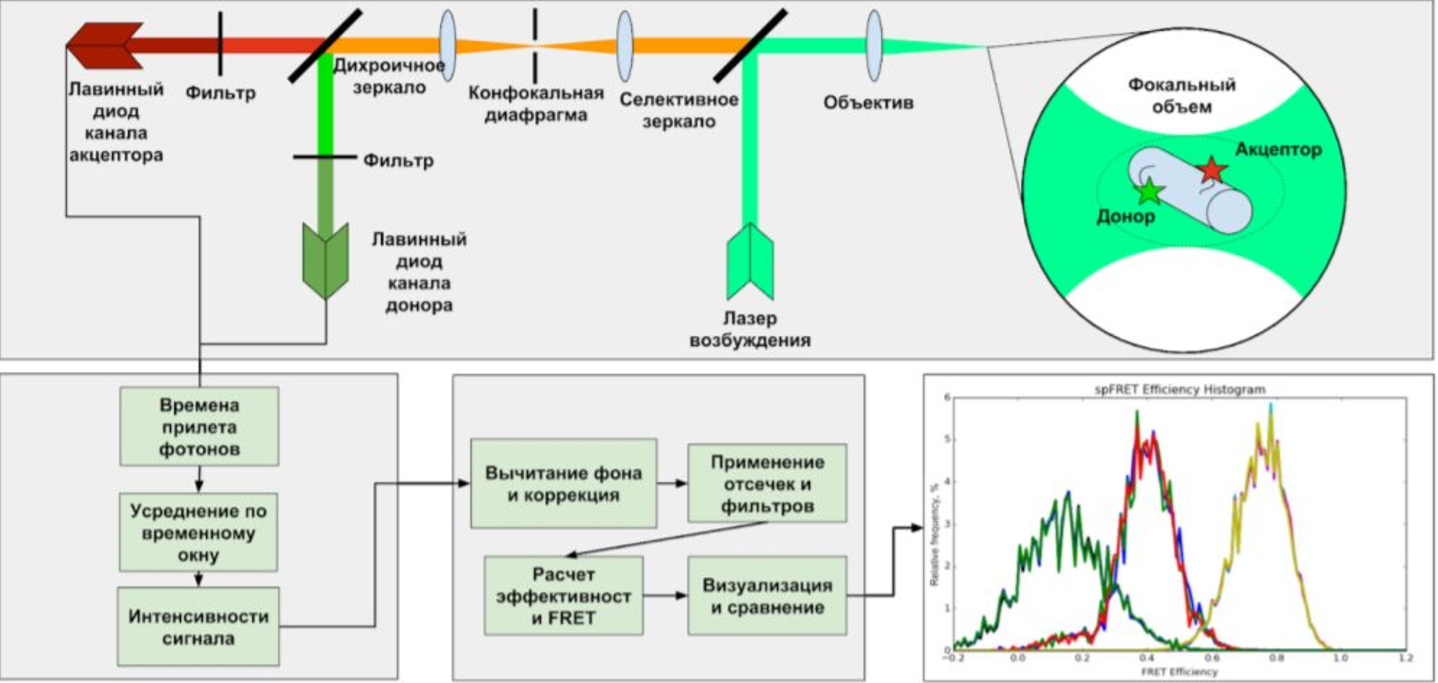
\includegraphics[width=\textwidth]{images/p1/part1_5_fret/part1_5_fret_f4.pdf}
    \caption[Схема экспериментов spFRET]{Схема экспериментов spFRET. Один лазер возбуждает флуоресценцию. Флуоресценция из конфокального объема собирается на лавинных фотодиодах. Времена прилета фотонов анализируются программным обеспечением микроскопа, либо специализированным ПО.}
    \label{fig:p1_5_fret:f4}
\end{figure}


\subsubsection{Подходы к измерению эффективности FRET}
Величина $E_{FRET}$, как следует из вышеприведенных формул, может быть рассчитана двумя способами, либо через время флуоресценции донора \cite{sisamakis_accurate_2010}, либо через измерение интенсивностей свечения донора и акцептора. Последний подход называется ратиометрическим подходом. 

Для того, чтобы измерить времена флуоресценции необходимо существенно более сложное оборудование. Порядок времен флуоресценции составляет порядка наносекунд, поэтому требуются лазерные источники и синхронизированные детекторы, способные работать в пикосекундном диапазоне. Такой подход реализован в методе TCSPC (Time Correlated Single Photon Counting). Он же используется в популярном методе микроскопии супер разрешения FLIM (fluorescence-lifetime imaging microscopy).
Важным преимуществом данного метода является отсутствие необходимости учитывать эффекты, связанные с мощностью осветителя, различными параметрами оптической системы и системы детекции, влияющими на корректировочные факторы. Наличие временного разрешения пикосекундрного диапазона, также позволяет эффективно проводить отсеивание шумовых всплесков в сигнале.

Ратиометрический подход может быть реализован с использованием более простого оборудования, например, конфокального микроскопа с лазером непрерывного излучения. Однако, этот подход чувствителен к шумовым эффектам, связанным с рассеянием света, колебаниям интенсивности лазера. Для соотнесения измеренных интенсивностей с реальными фотофизическими процессами необходимо предварительно измерить фактор детекции $\gamma$. Отдельной проблемой является то, что данный фактор может зависеть от конформационных изменений в молекулярной системе, так как квантовые выходы чувствительны к окружению флуорофоров.


\subsubsection{Подходы к измерению интенсивности флуоресценции spFRET от одиночных молекул}

Интенсивности флуоресценции в радиометрическом подходе, в зависимости от приборных возможностей, регистрируют либо в виде временного ряда, описывающего прилет отдельных фотонов (single photon counting), либо в виде некоторого сигнала, описывающего зависимость интенсивности от времени. В последнем случае прибор будет проводить усреднение (бинирование) сигнала с некоторым временным интервалом. В случае измерения spFRET в растворе, данный временной интервал необходимо выбирать с учетом кинетики проплывания частиц через фокальных объем микроскопа.
Для оценки времени проплывания частицы через фокальный объем можно использовать диффузионное соотношение:
 
\begin{equation}
    \tau \approx \langle x^2 \rangle / 2D
\end{equation}
    где $\tau$ - время проплывания, $D$ - коэффициент диффузии, $x$ - координата частицы вдоль одной из осей системы координат.
    
Для обработки непосредственно времен прилета фотонов также разработаны различные алгоритмы, позволяющие выделять внутри временного ряда события, связанные с проплыванием частиц и оценивать фоновых сигнал \cite{ingargiola_fretbursts_2016}. 
Оценку фонового сигнала можно проводить непосредственно анализируя правый край гистограммы распределения временных задержек между прилетом фотонов. Поскольку вероятность прилета фотонов за некоторый интервал времени описывается распределением Пуассона
\begin{equation}
    P[N(t)=k](t) = \frac{e^{-\lambda t} (\lambda t)^k}{k!}
\end{equation}
можно показать, что задержки распределены согласно экспоненциальному распределению:

\begin{equation}
    P(t)= \lambda e^{- \lambda t}
\end{equation}
где $\lambda$ - средняя частота детекции фотонов.
На практике распределение будет состоять из суммы распределения фонового сигнала и сигнала от проплывающих частиц.


% \begin{figure} [h!]
%     \centering
%     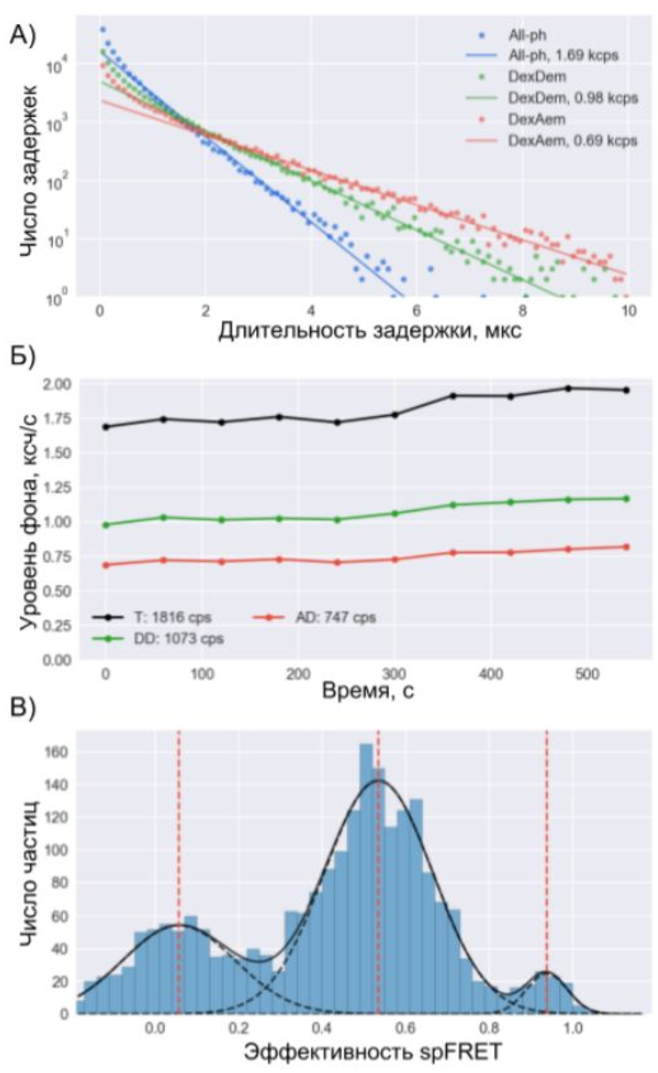
\includegraphics[width=100pt]{images/p1/part1_5_fret/part1_5_fret_f5.pdf}
%     \caption{А) гистограмма длительностей задержек между соседними фотонами в канале донора (зеленый), акцептора (красный), в обоих каналах (синий). Б) изменение уровня фона в ходе эксперимента. В) Типовая гистограмма эффективности spFRET со вписанными в нее тремя функциями Гаусса}
%     \label{fig:p1_5_fret:f5}
% \end{figure}

\subsubsection{Измерение фактора детекции}
При ратиометрическом измерении FRET вычисление истинного $E_{FRET}$ требует определения корректирующего фактора $\gamma$. Данный фактор позволяет перемасштабировать отношение регистрируемых интенсивностей сигнала в каналах донора и акцептора, чтобы учесть разницу в квантовых выходах красок и эффективности детекции фотонов от разных красок прибором. Также фактор детекции может изменяться целенаправленно варьируя параметры прибора для достижения большего разрешения в областях расстояния между метками большими или меньшими радиуса Ферстера \cite{gansen_structural_2009}. 

Для измерения параметра $\gamma$ можно использовать ряд экспериментальных методик. Квантовые выходы измеряют их сравнения с квантовыми выходами известных красителей \cite{williams_relative_1983}. Инструментальную часть фактора, $\gamma_{instrument}$, можно вычислить используя формулу:
\begin{equation}
    \gamma_{instrument} = \frac{m_{A}^{smF} m_{D}^{Abs} \Phi_{D}}{m_{D}^{smF} m_{A}^{Abs} \Phi_{A}}
\end{equation}
    где $m_{A}^{smF}$ и $m_{D}^{smF}$ - производные интенсивности флуоресценции акцептора и донора по концентрации для заданного лазера, $m_{A}^{Abs}$ и $m_{D}^{Abs}$ - производные поглощения акцептора и донора от концентрации, измеренные на длинне волны возбуждения донора, $\Phi_A$ и $\Phi_D$ квантовые выходы акцептора и донора. Более подробно методика описана в работе \cite{ferreon_interplay_2009}.

Альтернативой измерению фактора детекции в отдельных экспериментах (в том числе с применением спектрофотометра), является его измерение непосредственно во время эксперимента. Например, метод ALEX FRET (alternating laser excitation FRET) использует чередующиеся вспышки двух лазеров, возбуждающих поочередно донор или акцептор. Такой метод позволяет сразу определить стехиометрию красок в проплывающем комплексе. Измеряя эффективность переноса для комплексов с различной стехиометрией можно рассчитать фактор детекции \cite{lee_accurate_2005}. 

% \subsection{Детекция структурной гетерогенности в образце}
%     Чаще всего, результаты измерения эффективности spFRET анализируют путем построения частотных гистограмм (Рис. 5 В). Полученные распределения затем аппроксимируют Гауссовыми функциями, положение которых принимают за среднюю эффективность переноса энергии для субпопуляции частиц. Средняя эффективность переноса энергии затем может быть использована для оценки среднего расстояния между флуоресцентными метками. Помимо средней эффективности, информацию об исследуемой системе можно получить из формы и ширины распределения эффективностей spFRET [60,61]. Уширение распределений может свидетельствовать как о статической структурной гетерогенности образца, так и о динамической структурной гетерогенности образца: под статической гетерогенностью понимают наличие в образце смеси частиц с разными расстояниями между метками, изменение расстояний при этом либо не происходит, либо происходит на временах, значительно превышающих времена диффузии частиц сквозь фокальный объем. О динамической гетерогенности говорят в случае наличия конформационной подвижности молекул, приводящей к тому, что эффективность spFRET изменяется в ходе диффузии частицы сквозь фокальный объем. Возможность наблюдения динамической гетерогенности позволяет судить о характерных временах конформационных перестроек в макромолекулах.%not edited
%     В работе [62] был предложен оригинальный подход для определения наличия динамической гетерогенности в образце, основанный на определении вариабельности сигнала в процессе проплывания частицы через фокальный объем. Наличие быстрых структурных перестроек внутри образца должно приводить к увеличению стандартного отклонения измеренной эффективности spFRET для каждой детектируемой вспышки флуоресценции. В случае отсутствия подвижности в образце, отклонения в сигнале будут вызваны лишь случайным шумом, который достаточно просто оценить. Любая последовательность из $n$ фотонов в канале флуоресценции донора подчиняется биномиальному распределению с вероятностью успеха равной эффективности FRET ( $E^*=\frac{N_a}{N_a+N_d}$ , где $N_x$ - число фотонов в канале донора или акцептора, $n$ - общее число фотонов). Исходя из этого, стандартное отклонение сигнала в канале акцептора будет описываться формулой $\sigma_{Na}=\sqrt{n E^* (1-E^*)}$ , а стандартное отклонение эффективности spFRET будет подчиняться формуле%not edited
% \begin{equation}
%     \sigma_{E^*}=\sqrt{\frac{ E^* (1-E^*)}{n}}
% \end{equation}
%     Эта кривая (пунктирная линия на Рис. 6) является ориентиром для оценки стандартного отклонения исследуемого сигнала. Для каждой вспышки флуоресценции рассчитывается стандартное отклонение эффективности spFRET:%not edited
% \begin{equation}
%     \sigma_i = \sqrt{\frac{1}{N_i}\sum_{j=1}^{Ni} (\epsilon_{ij} - \mu_i)^2} , где \mu_i = \frac{1}{Ni}\sum_{j=1}^{Ni} \epsilon_{ij}
%     \end{equation}
%     и строится двумерная гистограмма распределения стандартного отклонения от величины эффективности переноса энергии (Рис. 6). При этом, если среднее стандартное отклонение превышает ожидаемое из биномиального распределения, можно говорить о наличии динамической гетерогенности в образце, которая приводит к уширению профилей эффективности spFRET.%not edited
    
%  \begin{figure} [h!]
%      \centering
%      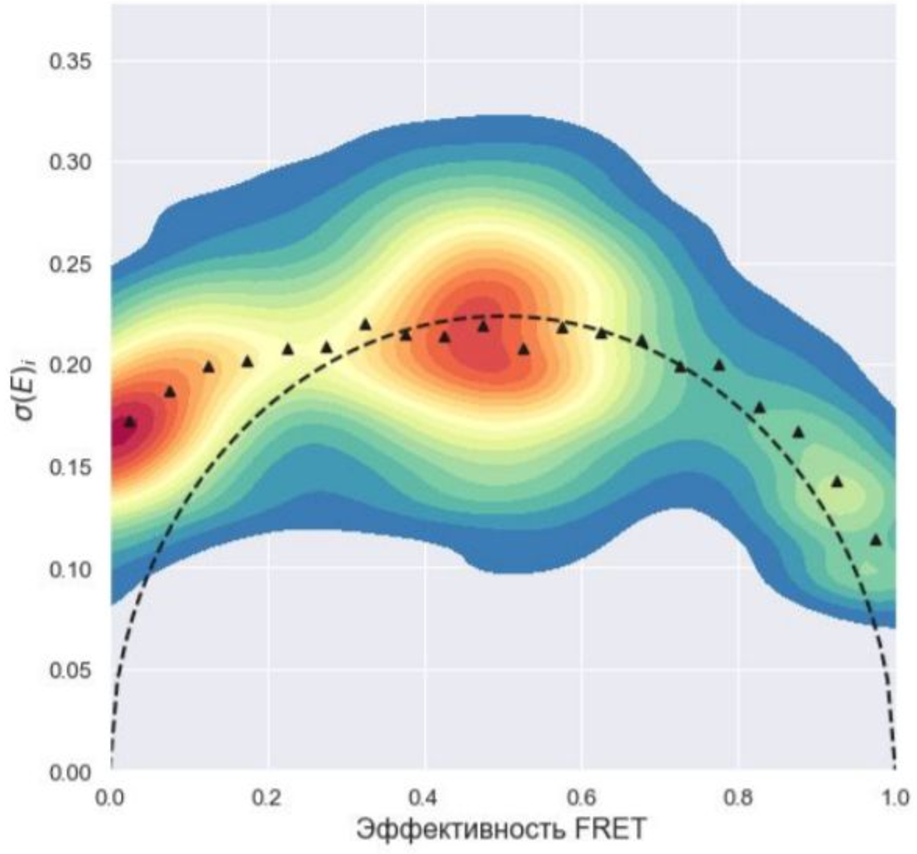
\includegraphics[width=\textwidth]{images/p1/part1_5_fret/part1_5_fret_f6.pdf}
%      \caption{Двумерная гистограмма распределения стандартного отклонения величины эффективности spFRET. Пунктиром показана линия ожидаемого стандартного отклонения для сигнала, распределенного биномиально (Формула 10).}
%      \label{fig:p1_5_fret:f6}
%  \end{figure}
 
    % На приведенной двумерной гистограмме (Рис. 6) видно, что для низких и высоких величин эффективности FRET стандартные отклонения превышают теоретическую оценку. Этот эффект может свидетельствовать о наличии быстрых перестроек в этих субпопуляциях частиц, но также может быть связан с тем, что метод оценки вариабельности вспышек не учитывает уровень фона и другие корректировочные коэффициенты (см. Формулу 3).%not edited













\subsection{Методы геномного анализа в исследовании структуры хроматина}
% сделать на основе https://docs.google.com/document/d/1GcTfefw2HnJGGnGmaJP5w2JN1Jy8X2EyCjyOlxEbagU/edit?usp=sharing

    Для определения наличия физического контакта между последовательностями ДНК в трехмерной структуре генома были разработаны методы семейства -С: 3С, 4С, 5С, Hi-C \cite{fraser_overview_2015}. Эти методы основаны на химическом ``сшивании'' контактирующих в хроматине участков, фрагментации ДНК с образованием ``сшитых'' пар, лигирования фрагментов в этих парах с образованием гибридных молекул ДНК, детекции гибридных молекул (обнаружение молекулы, состоящей из последовательности А и последовательности В, говорит о физическом контакте локусов этих последовательностей в ДНК).
    Существует понятие ``разрешения'' метода Hi-C (см. Таблицу \ref{tab:p1:hic}). Его можно определить как минимальное расстояние (в парах оснований) между участками, на котором они отображаются на тепловую карту в разные ее точки (пиксели). Величина разрешения зависит от величины фрагментов, на которые рестриктазы разрезают ДНК (то есть от особенностей используемых рестриктаз, размеров и встречаемости в геноме их сайтов рестрикции), и от размера бина, выбираемого на стадии обработки данных Hi-C, но не полностью произвольного: для получения тепловой карты, адекватно представляющей трехмерную структуру изучаемого генома, необходимо выбирать размеры бинов из определенного диапазона, зависящего от размеров хромосом, глубины секвенирования и качества NGS-библиотеки \cite{pal_hi-c_2019}. От разрешения метода Hi-C зависит то, какие структуры в хроматине он может выявить. Оригинальный протокол метода, описанный в статье 2009 года \cite{lieberman-aiden_comprehensive_2009}, позволял достичь разрешения 4kb и выявлял, соответственно, в трехмерной структуре генома компартменты A и B (соответствующие активному и неактивному хроматину). В протоколах Hi-C, разработанных позже, достигалось, благодаря использованию других рестриктаз, большее разрешение - до одной килобазы. Это позволяло обнаружить так называемые топологически ассоциированные домены (ТАДы) \cite{dixon_topological_2012} и взаимодействия конкретных последовательностей друг с другом - то есть, физические контакты регуляторных элементов с регулируемыми ими генами, реализованные, как полагают современные исследователи, запетливанием ДНК. Однако этих разрешающих способностей все равно не достаточно, чтобы изучить супрануклеосомный уровень, на котором ранее предполагалось существование 30-нанометровой фибриллы \cite{pal_hi-c_2019}.
    
    Пролить свет на этот уровень смог метод Micro-C — модификация метода Hi-C, предполагающая использование на этапе фрагментации ДНК микрококковой нуклеазы, которая уничтожает линкерные участки, оставляя одни  нуклеосомы (этот метод можно рассматривать как синтез метода позиционирования нуклеосом с помощью микрококковой нуклеазы - MNase-seq \cite{cui_genome-wide_2012} - и Hi-C \cite{hsieh_mapping_2015}. Это позволяет оценивать частоту взаимодействия отдельных нуклеосом друг с другом, то есть разрешение метода достигает неизученного супрануклеосомного уровня (между 200bp и 4kb), устраняя так называемый ``пробел в разрешении'' (resolution gap). Интересно, что метод Micro-C тоже не обнаружил 30-нанометровую фибриллу, еще раз доказав необходимость дальнейших исследований структуры хроматина супрануклеосомного уровня. В работе, в которой впервые был предложен метод Micro-C, изучался геном дрожжей - \textit{S. cerevisiae}. 
    
    Параллельно Micro-C был разработан другой метод Hi-C высокого разрешения - in situ DNase Hi-C. С его помощью можно получить данные с разрешением около 1kb \cite{ramani_mapping_2016}. Однако этот метод, основанный на использовании фермента DNase I, неспецифически фрагментирующего ДНК на тетрануклеотиды, не является конкурентным для Micro-C в области изучения супрануклеосомной структуры хроматина, так как не уничтожает линкерную ДНК и, соответственно, не позволяет в отличие от Micro-C простым способом получить данные о частоте взаимодействия нуклеосом друг с другом. 
    Сам протокол Micro-C модифицировался после его изобретения. Примером могут служить работы \cite{hsieh_micro-c_2016} и \cite{ohno_sub-nucleosomal_2019}, в которых были впервые представлены модификации Micro-C:  Micro-C XL и Hi-Co, соответственно. Micro-C XL - метод, позволяющий получить качественные данные в мононуклеосомном разрешении, это достигается путем снижения шума за счет изоляции нерастворимого хроматина и использования помимо формальдегида длинных сшивающих агентов (кросслинкеров) - например, DSG и EGS. Метод Hi-Co специфичен тем, что с его помощью можно определить ориентацию нуклеосом (``O''  в названии - от Orientation). Это достигается с помощью особой биоинформатической обработки и использования не просто секвенирования спаренных концов, а секвенирования спаренных концов с тэгами (PET - paired-end tags \cite{fullwood_next-generation_2009}).
    
    \begin{table}[p]
\caption{Увеличение разрешения Hi-C подобных методов, благодаря использованию менее специфичных рестриктаз.}
	\label{tab:p1:hic}	
	\begin{tabularx}{\textwidth} { 
  | >{\raggedright\arraybackslash}X 
  | >{\centering\arraybackslash}X 
  | >{\raggedleft\arraybackslash}X 
  | >{\raggedleft\arraybackslash}X |}
  \hline
Протокол Hi-C & Рестриктазы & Сайты рестрикции & Размер сайта рестрикции\\
	\hline

Классический (Lieberman-Aiden et al., 2009) & HindIII, NcoI & AAGCTT, CCATGG & 6 пн \\
\hline
Sexton et al., 2012, Rao et al., 2014 & Dpn-II & GATC & 4 пн \\
\hline
COLA (Darrow et al., 2016) & CviJI & RCGY, R=A/G, Y=C/G & 3 пн \\
\hline
Micro-C (Hsieh et al., 2016) & MNase & Отсутствует. Эндо/экзо нуклеаза, почти полностью уничтожает линкерные участки ДНК &  - \\
\hline
in situ DNAse Hi-C (Ramani et al., 2016) & DNAse I & Отсутствует. Режет ДНК на тетранукеотиды & -  \\
\hline
\end{tabularx}
	 
\end{table}
    
    Следует отметить, что все методы -C являются статистическими и вероятностными, приблизительно оценивающими частоту взаимодействия большого количества фрагментов ДНК. Для получения биологически значимой информации с помощью метода Hi-C вообще и, в частности Micro-C, необходим тщательный биоинформатический анализ матриц взаимодействия: фильтрация  и нормализация данных, учет того — использовалась в методе клеточная популяция или единичная клетка (Single-Cell Hi-C/Micro-C \cite{nagano_single-cell_2013}). Для изучения супрануклеосомной структуры хроматина с помощью Micro-C необходимо дополнительно прибегнуть к его молекулярному моделированию с учетом последних достижений в вычислительной биофизики.

\begin{figure} [h!]
    \centering
    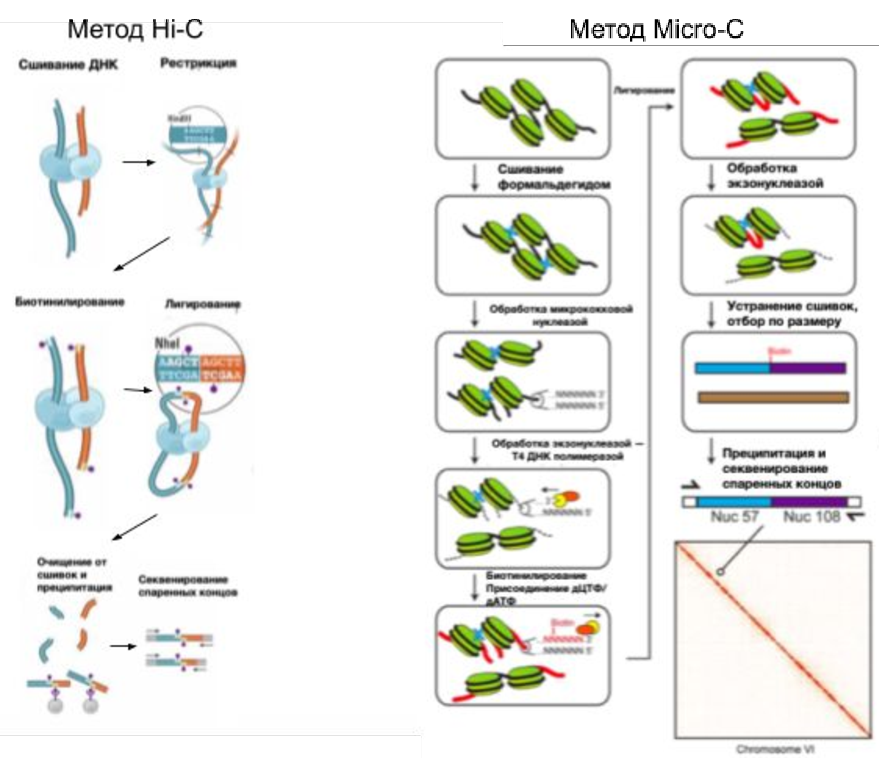
\includegraphics [width=\textwidth]{images/p1/part1_5_genome/p1_5_genome_f5.pdf}
    \caption[Методы ``захвата конформации хроматина''.]{Методы ``захвата конформации хроматина'' (chromatin conformation capture), сравнение Hi-C и Micro-C. Адаптировано из \cite{lieberman-aiden_comprehensive_2009} и \cite{hsieh_mapping_2015}.}
    \label{fig:p1_5_genome:f5}
\end{figure}


    Появление методов секвенирования нового поколения дало огромное преимущество большинству методов эпигеномики, позволяющим получать данные о местах расположения нуклеосом, в том числе с гистоновыми вариантами и с определенными пост-трансляционными метками гистонов. 

    Метод MNase-seq позволяет получить данные о расположении единичных нуклеосом. В методе используется микрококковая нуклеаза, которая обладает экзо- и эндонуклеазными активностями. После работы нуклеазы, нуклеосомальная ДНК освобождается от гистонов и секвенируется. Далее прочтения картируются на референсный геном.       На данный момент в публичном доступе накоплено большое количество экспериментальных наборов данных для клеток разных организмов и из разных тканей человека (110 наборов данных по данным сайта \url{https://generegulation.org/nucleosome-positioning-database/}).
    К основным проблемам использования методов Mnase-seq относится огромное количество получаемых с одного эксперимента прочтений - порядка 200-400 млн для клеточных линий человека. Для достижения оптимального разрешения позиционирования нуклеосом в человеческих клетках для сравнения здоровых и больных требуется порядка 1-4 млрд прочтений \cite{teif_nucleosome_2016}. Обычно эксперименты MNase-seq выполняют на нескольких тысячах клеток, такой усредненный нуклеосомальный профиль характеризует ансамбль клеток, а не частные состояния клеток. Специализированная база данных NucMap включает 798 экспериментальных наборов данных MNase-seq из 477 образцов для 15 видов живых организмов \cite{zhao_nucmap:_2019}. Для дрожжей существует метод СС-seq, позволяющий определять позиционирование нуклеосом с большей точностью, чем MNase-seq \cite{brogaard_map_2012}. Суть метода в ведении специальной мутации в гистоны, в результате которой вблизи центра нуклеосомы появляется остаток цистеина. Боковая цепь цистеина используется для реакции со специальными химическими агентами, которые разрезают ДНК в центре нуклеосомы. Далее методами секвенирования определяется положение разреза и, следовательно, центра нуклеосомы.
    Методы ChIP-seq осуществляют анализ ДНК-белковых взаимодействий. 
    В открытом доступе находится большое количество наборов данных ChIP-seq гистоновых модификаций, включая метки энхансеров и промотеров, например, ChIPBase v.2.0 2466 датасетов, IHEC Data Portal - несколько тысяч образцов из разных человеческих органов, ChIP-Atlas - данные из 96000 экспериментов. Также ChIP-Atlas позволяет ответить на следующие вопросы: какие белки были связаны с определенной последовательностью ДНК, какие гены регулируются данным белком, какие белки колокализированы с данным, а также позволяет предсказывать белки, связанные с данными геномными локусами и генами (in silico ChIP).
    Важная модификация метода ChIP-seq - метод Mnase ChIP-seq заключается в отщеплении свободных п.н. (линкерной ДНК) микрококковой нуклеазой до этапа иммунопреципитации. В результате образуются фрагменты 20-70 п.н., позволяющие строить нуклеосомальные профили и выявлять сайты связывания транскрипционных факторов высокого разрешения.  Было отмечено, что MNase-ChIP-seq также позволяет увеличить воспроизводимость результатов по сравнению с ультразвуковой фрагментацией в методе ChIP-seq \cite{wedel_genome-wide_2017}. 
    В работе \cite{rhee_subnucleosomal_2014} с помощью методов ChIP-exo и MNase-seq было показано наличие субнуклеосомальных структур (гексасомы, нуклеосомы с единично представленными гистонами типов H2A, H2B, H3, H4) \textit{in vivo} и сделаны предположения о влияния последовательности ДНК на образование таких структур. 

    В работе \cite{quintales_comparative_2015} проведено сравнение обработки сырых данных экспериментов: MNase-seq, ChIP-seq и метода химического расщепления ДНК в месте диадной оси, используя разные стратегии секвенирования (одноконцевое и парноконцевое), с помощью разработанной программы NUCwave. Было показано, что обработка данных парноконцевого секвенирования MNase-seq наиболее точно определяет известные позиции нуклеосом и превосходит другие сырые данные для построения карт расположения нуклеосом.

\begin{figure} [h!]
    \centering
    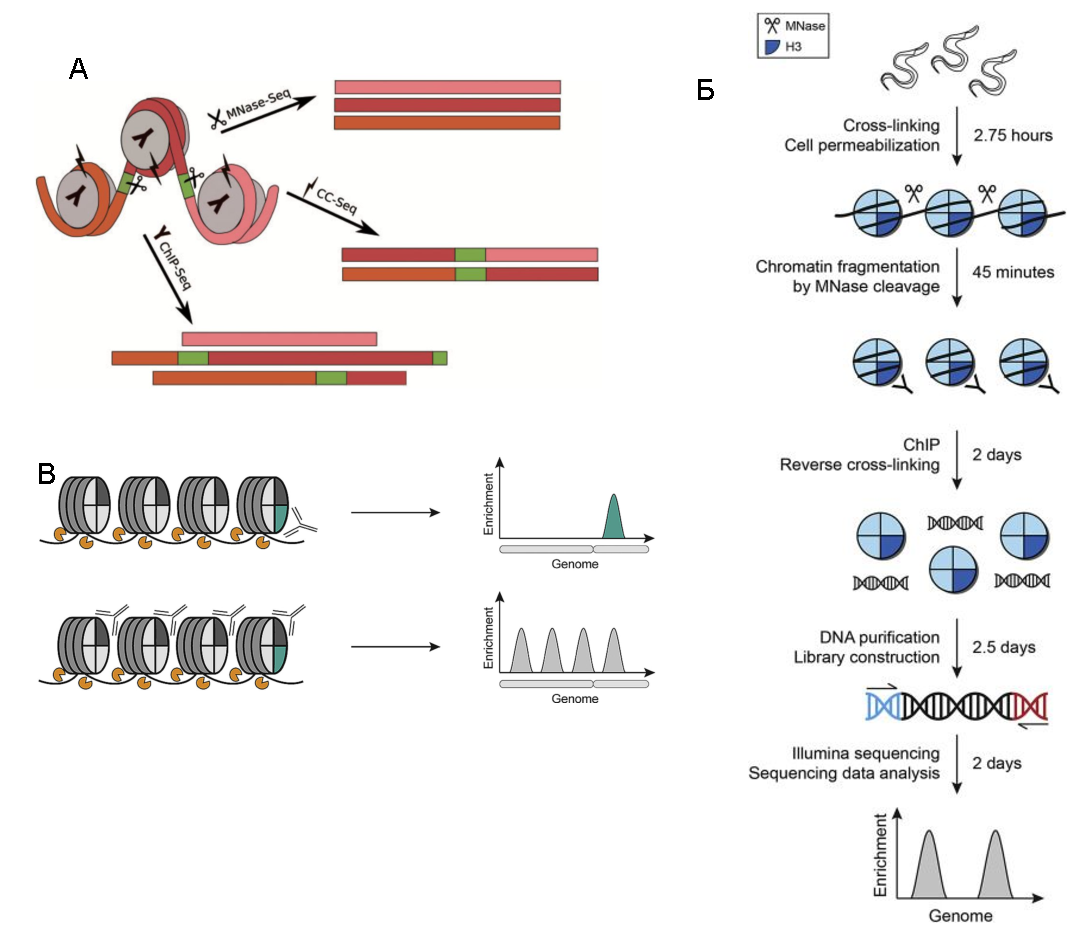
\includegraphics [width=\textwidth]{images/p1/part1_5_genome/p1_5_genome_f6.pdf}
    \caption[Методы эпигеномики нуклеосомного разрешения]{Методы эпигеномики нуклеосомного разрешения: А) MNase-seq, ChIP-seq, CC-seq. Б-В) MNase-ChIP-seq. Адаптировано из \cite{quintales_comparative_2015} и \cite{wedel_genome-wide_2017}.}
    \label{fig:p1_5_genome:f6}
\end{figure}



















%\subsection{Кристаллография}
%\subsection{Электронная микроскопия}
%\subsection{ЯМР}
%\subsection{Малоугловое рассеяние}
%\subsection{Методы дейтеро-водородного обмена}
%\subsection{Лазеры на свободных электронах}




\section{Выводы главы \ref{chapt1_mod_methods}}
Исследование структуры многих биомакромолекулярных комплексов испытывает затруднения как при применении стандартных методов структурной биологии, так и при попытках атомистического моделирования на основе расчета атом-атомных взаимодействий. Методы интегративного моделирования, в ходе расчетов учитывающие как физические взаимодействия между атомами, так и экспериментальные данные различной природы, являются перспективным подходом для построения структурно-динамических моделей биомакромолекулярных комплексов. В главе предложены подходы по моделированию ДНК-белковых комплексов на основе моделей анизотропной гибкости ДНК с учетом разнородных экспериментальных данных.
%\subsection{Положения выносимые на защиту}
%положения выносимые на защиту
% \begin{enumerate}
%   \item Охарактеризовано направление интегративного моделирования, как набор подходов атомистического и огрубленного моделирования, позволяющих создавать структурно-динамические модели биомакромолекул и их комплексов на основе наборов разнородных экспериментальных данных.
%   \item Предложены комплексные подходы по моделированию структуры и динамики ДНК-белковых комплексов с учетом разнородных экспериментальных данных, в том числе низкого информационного содержания.
% \end{enumerate}
 
           % Глава 1 - методы моделирования и их место - вводная глава.
\chapter[Применение методов молекулярной динамики для изучения нуклеосом]{Применение методов молекулярной динамики для изучения нуклеосом\footnote{При подготовке данного раздела диссертации использованы следующие публикации, выполненные автором лично или в соавторстве, в которых, согласно Положению о присуждении ученых степеней в МГУ, отражены основные результаты, положения и выводы исследования: \cite{shaytan_coupling_2016,hada_histone_2019,bass_effect_2019,armeev_linking_2019,gribkova_investigation_2017,el_kennani_ms_histonedb_2017,shaytan_trajectories_2016,shaytan_coupling_2016,draizen_histonedb_2016,armeev_nucleosome_2016,shaytan_nucleosome_2015,armeev_conformational_2015,armeev_molecular_2015}.}} \label{part2_supermd}

Данная глава иллюстрирует современные возможности суперкомпьютерного моделирования методом атомистической молекулярной динамики для получения и анализа структурно-динамических моделей биомакромолекулярных комплексов на основе информации об их статических структурах, получаемых методами структурной биологии.
Глава посвящена расчету и анализу молекулярно-динамических моделей ключевых нуклеопротеиновых комплексов хроматина эукариот - нуклеосом.
Во введении дан широкий обзор литературы по динамике нуклеосом и их роли в функционировании хроматина. В сутевой части главы приводятся результаты по рекордно долгим вычислениям траекторий молекулярной динамики в микросекундном диапазоне (в том числе свыше 10 микросекунд). Предложены оригинальные алгоритмы анализа динамического поведения нуклеосом, на основе которых проанализирован ряд физиологически важных динамических мод нуклеосом.
Результаты приведенные в данной главе основаны на статьях  \cite{shaytan_coupling_2016,hada_histone_2019,bass_effect_2019,armeev_linking_2019,gribkova_investigation_2017,el_kennani_ms_histonedb_2017,shaytan_trajectories_2016,shaytan_coupling_2016,draizen_histonedb_2016,armeev_nucleosome_2016,shaytan_nucleosome_2015,armeev_conformational_2015,armeev_molecular_2015}, тезисах  \cite{armeev_integrative_2020,gribkova_construction_2019,armeev_analyzing_2019,shaytan_microsecond_2017,shaytan_nucleosome_2016,shaytan_polymorphism_2015,shaytan_combined_2015}, а также включают новые результаты.

\section{Введение в структуру и динамику нуклеосом}
\textit{Данный раздел написан по материалам собственной обзорной статьи \cite{armeev_linking_2019}}.

%\todo{2S - сюда нужно вставить переведенные текст с картинками materials\/cosb\_2019\/paper\_rev\_v10.docx, картинки нужно засунуть в гугл Draw (папка p2) - там перевести наложив поверх английского текста русский. Ссылки на литературу уже загружены в зотеро. Все заголовки начинать с уровня subsection и далее}


% \section{Реферат}

%     Нуклеосомы являются фундаментальными единицами уплотнения хроматина, которые обертывают около $\sim$ 150 пар оснований ДНК вокруг октамера гистоновых белков. Их повсеместное присутствие в ядре клетки с тех пор, как первые эукариоты заставили хроматиновый аппарат совместно развиваться и научиться использовать различные способы динамики нуклеосом и ощущать различия в составе нуклеосом. Изменения последовательностей гистонов или ДНК, посттрансляционные модификации (PTM) гистонов, рекрутирование белков хроматина модулируют динамику нуклеосом и обеспечивают эпигенетическую регуляцию путей обработки ДНК (транскрипция, репликация, репарация и т. Д.). Наше понимание этого сложного взаимодействия между составом, динамикой и функционированием нуклеосом постоянно развивается благодаря новым знаниям и открытиям. В этом обзоре мы выделяем последние достижения в этой области, пытаясь организовать их в единую структуру.

% \subsection{Введение}

    Жизнь эукариотических клеток полностью управляется пространственно-временной организацией хроматина внутри ядер клеток. Хроматин не только компактизует ДНК, но и служит средой для расшифровки и интерпретации генетической информации \cite{van_holde_chromatin_1989}. Основной структурной единицей организации хроматина является нуклеосома - повторяющаяся единица из примерно 200 пар оснований ДНК, организованная гистоновыми белками \cite{olins_spheroid_1974,kornberg_chromatin_1974-1} (Рис. \ref{fig:part2_1_f1}a). Центральные 145–147 пар оснований ДНК образуют коровую частицу нуклеосомы, или нуклеосомный кор (NCP, nucleosome core particle), плотно наматываясь на октамер гистонов в виде $\sim$1,7 витка левой суперспирали \cite{luger_crystal_1997,tan_nucleosome_2011}. Линкерные сегменты ДНК фланкируют NCP. Канонический октамер гистонов состоит из двух пар идентичных гистоновых димеров H3-H4 и H2A-H2B, образованных коровыми гистонами H3, H4, H2A и H2B, соответственно (Рис. \ref{fig:part2_1_f1}a) \cite{draizen_histonedb_2016}. Симметрия октамера наделяет NCP осью псевдосимметрии второго порядка, которая определяет расположение центра ДНК - диады нуклеосом. Все четыре типа гистонов, вероятно, имеют общее эволюционное происхождение и имеют сходную структуру  \cite{malik_phylogenomics_2003,bhattacharyya_archaeal_2018} (Рис. \ref{fig:part2_1_f1}б). Гистоны также подразделяются на основные ``канонические'' гистоны (депонируются на ДНК при репликации) и альтернативные варианты гистонов, которые синтезируются в течение клеточного цикла и могут быть тканеспецифичными \cite{draizen_histonedb_2016}. Дополнительные уровни вариабельности нуклеосом обеспечиваются репертуаром посттрансляционных модификаций гистонов (ПТМ) \cite{bowman_post-translational_2015} и вариаций внутри последовательностей ДНК (Рис. \ref{fig:part2_1_f1}в).

С годами стало ясно, что нуклеосомы претерпевают множество функционально важных структурных и динамических перестроек во время всех ключевых процессов происходящих в хроматине (транскрипция, репликация, репарация ДНК и т.д.) \cite{zlatanova_nucleosome_2009,chen_asymmetric_2017}. Более того, способность нуклеосом претерпевать определенные типы конформационных переходов разумно используется многими белками хроматина, включая ремоделирующие хроматин \cite{sinha_distortion_2017,liu_mechanism_2017,ranjan_h2a_2015-1}, факторы транскрипции \cite{laptenko_p53_2011,zaret_pioneer_2016}, шапероны \cite{valieva_large-scale_2016}, РНК-полимеразы \cite{gaykalova_structural_2015} и т.д. С момента появления первых эукариот около 2 миллиардов лет назад биологические процессы ядра приспосабливались к структуре нуклеосомы, используя тонкие детали ее динамики. Одновременно с диверсификацией репертуара нуклеосом с помощью вариантов гистонов и их ПТМ белки хроматина также диверсифицировались и эволюционировали, чтобы различать разные нуклеосомы по их структурным и динамическим характеристикам. Это тонкое взаимодействие между составом нуклеосом, структурой, функциональной динамикой и взаимодействиями с белками хроматина формирует основы многих регуляторных путей, происходящих в хроматине.

    Ниже мы очертим концептуальную схему для понимания различных режимов структурной динамики нуклеосом и классифицируем основные факторы, которые влияют на эти режимы. 

\begin{figure} [H]
    \centering
    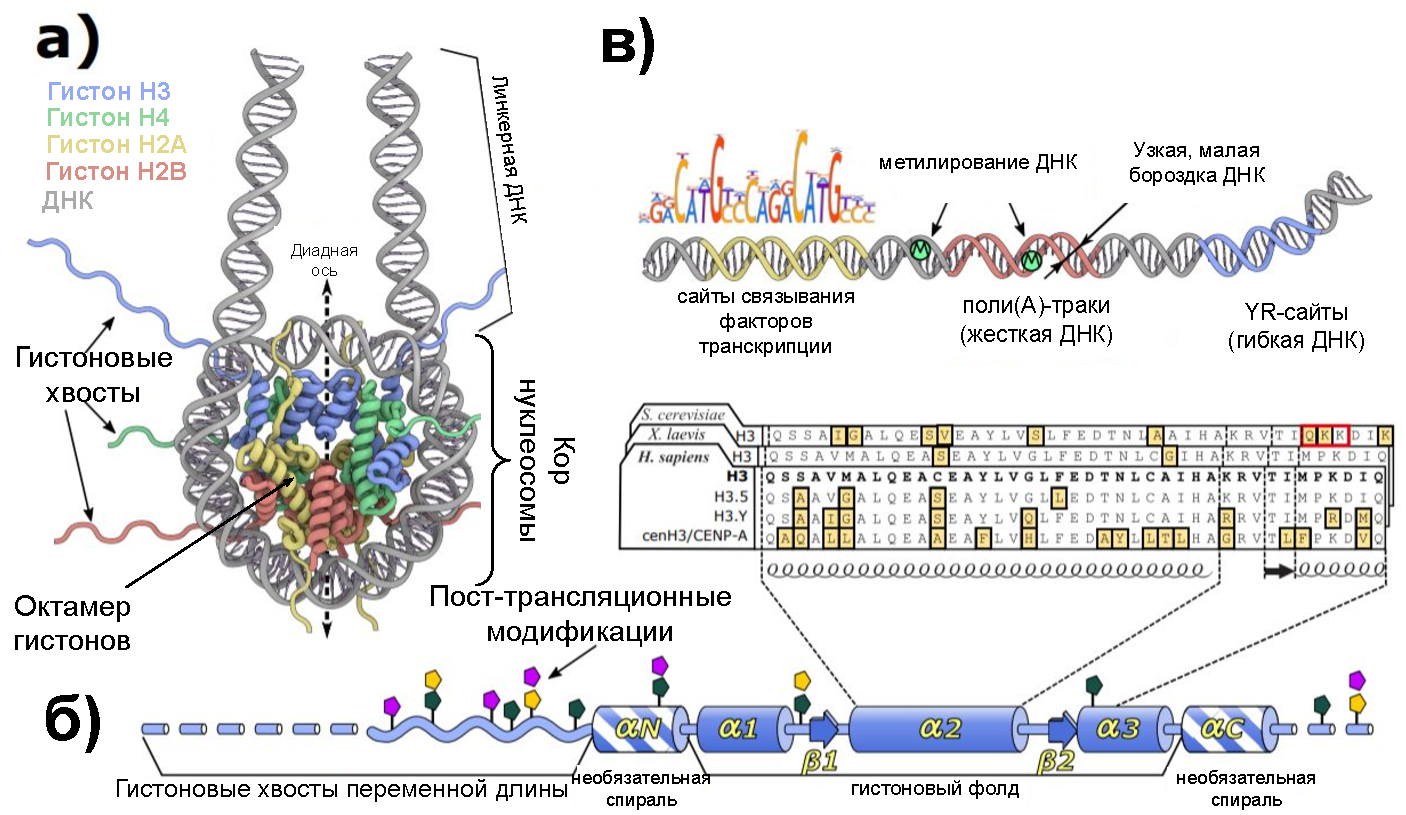
\includegraphics [width=\textwidth]{images/p2/cosb/part2_1_f1.pdf}
    \caption[Структура и вариабельность нуклеосомы]{(a) Структура нуклеосомы состоит из коровой частицы нуклеосомы (NCP), фланкированной линкерными сегментами ДНК. Коровая частица образована октамером гистонов, вокруг которого обернуты 145–147 пар оснований ДНК в виде левой суперспирали. Октамер состоит из двух пар гетеродимеров гистонов (H3-H4 и H2A-H2B) и обладает осью псевдосимметрии второго порядка (диадной осью), проходящей через центральную пару оснований нуклеосомной ДНК (диаду). Неструктурированные гистоновые хвосты отходят от глобулярной части белков. Малая бороздка ДНК обращена к октамеру гистонов в 14 специально предназначенных для этого сайтах связывания (в каждом сайте связывания боковая цепь остатка аргинина вставлена в малую бороздку). 
    (б) Схема типичной структуры гистонового белка: гистоновый фолд (спирали $\alpha$1, $\alpha$2 и $\alpha$3, листы $\beta$1 и $\beta$2) с необязательными спиралями $\alpha$N, $\alpha$C и гистоновыми хвостами переменной длины. Гистоновые ПТМ могут располагаться по всей длине белка и играть важную роль в функционировании хроматина, обеспечивая эпигенетическую разметку. Вариации гистонового сиквенса существуют как между организмами, так и внутри организма (гистоновые варианты).
    (в) ДНК - ключевой компонент нуклеосомы. Конкретные последовательности ДНК могут обеспечивать присутствие сайтов связывания факторов транскрипции в областях нуклеосомной ДНК, повышенную жесткость и/или изменения геометрии ДНК.}
    \label{fig:part2_1_f1}
\end{figure}



\subsection{Обзор динамических мод нуклеосом}

    Внимание на динамическую природу нуклеосом впервые было обращено в контексте отворачивания ДНК от октамера гистонов \cite{polach_mechanism_1995} (Рис. \ref{fig:part2_1_f2}a, в центре). Результаты экспериментов по ферментативному расщеплению ДНК \cite{polach_mechanism_1995}, измерению FRET \cite{li_nucleosomes_2004}, крио-ЭМ \cite{bilokapic_histone_2018} свидетельствуют о возможности откручивания ДНК (иногда называемом раскручиванием или дыханием ДНК). Данные процесс важен для доступа факторов транскрипции \cite{zaret_pioneer_2016,li_nucleosomes_2004} и РНК-полимераз \cite{bondarenko_nucleosomes_2006} к последовательности ДНК. Позднее выяснилось, что откручивание ДНК может происходить вместе с раскрытием димера H2A-H2B (состояние ``бабочка'') \cite{bohm_nucleosome_2011} или его полной диссоциацией (с образованием гексасомы), что часто происходит при транскрипции \cite{kireeva_nucleosome_2002}. Частично собранные нуклеосомы (также называемые субнуклеосомными структурами), такие как тетрасома или гемисома (полунуклеосома) также эффективно способствуют отворачиванию ДНК \cite{rychkov_partially_2017}. Недавно с использованием метода ChIP-exo было показано, что такие структуры широко распространены в динамическом хроматине в масштабе всего генома  \cite{rhee_subnucleosomal_2014}. В то время как тетрасомы могут возникнуть из-за потери двух димеров H2A-H2B нуклеосомой, динамические пути, ведущие к гемисомам, не совсем ясны. Новые экспериментальные данные подтверждают идею о том, что сборка нуклеосом \textit{in vivo} во время репликации ДНК происходит через депонирование тетрамеров H3-H4 (два димера H3-H4, взаимодействующие через четырехспиральную связку) с помощью фактора сборки хроматина 1 (CAF1) \cite{sauer_insights_2017,mattiroli_dna-mediated_2017}. После этого к ним присоединяются димеры H2A-H2B. Следовательно, маловероятно, что гемисомы образуются во время регулярной сборки нуклеосом. Расщепление нуклеосом на полунуклеосомы во время транскрипции - еще одна гипотеза (рассмотренная в \cite{zlatanova_nucleosome_2009}). Хотя есть некоторые споры, частным случаем статической структуры полунуклеосом могут быть центромерные нуклеосомы \textit{S. cerevisiae} \cite{henikoff_remarkable_2017}, которые также могут быть воссозданы \textit{in vitro} в особых условиях \cite{furuyama_reconstitution_2013}. В то время как нуклеосома в отсутствие внешнего сверхспирального стресса содержит ДНК в виде левосторонней суперспирали \cite{bancaud_structural_2006}, тетрасомы или гемисомы демонстрируют повышенную тенденцию к адаптации правостороннего состояния. Вероятно, так обстоит дело с центромерными нуклеосомами пекарских дрожжей [\textit{ibid.}] и тетрамерами гистонов архей \cite{marc_archaeal_2002}.



    В левой части рисунка \ref{fig:part2_1_f2} мы сгруппировали динамические режимы с меньшей величиной конформационных изменений (``компактная нуклеосома''), которые, тем не менее, функционально важны. Октамер гистона способен к ``расщеплению'' - изменению расстояния между двумя половинками нуклеосомы вдоль оси суперспирали ДНК. Экспериментально это наблюдалось на  нуклеосомах \cite{ngo_nucleosomes_2015,falk_cenp-c_2015} и может быть связано со скольжением витков ДНК относительно друг друга \cite{falk_cenp-c_2016}. Недавно наше понимание динамики октамера было дополнительно расширено за счет концепции пластичности октамеров на уровне отдельных димеров гистонов - точечные сшивки внутри димера H3-H4 ограничивает его деформируемость и ингибируют передвижение нуклеосом ремоделером SNF2h \cite{sinha_distortion_2017}. Наконец, ДНК в нуклеосоме - это компонент, который проявляет конформационную изменчивость. Октамер может скользить по ДНК, изменяя ротационное и трансляционное позиционирование ДНК \cite{shaytan_hydroxyl-radical_2017,shaytan_structural_2018}. Этот процесс сильно зависит от последовательности ДНК (обзор см. в \cite{eslami-mossallam_nucleosome_2016}) и включает локальные деформации ДНК, такие как дефекты скручивания \cite{edayathumangalam_nucleosomes_2005}. В линкерной области ДНК более гибкая, чем остальная часть ДНК \cite{gansen_structural_2009}. Благодаря такой высокой мобильности, комплексы нуклеосом с линкерным гистоном могут образовывать ансамбль различных конфигурации (см. обзор в \cite{ozturk_toward_2018}).


\begin{figure} [H]
    \centering
    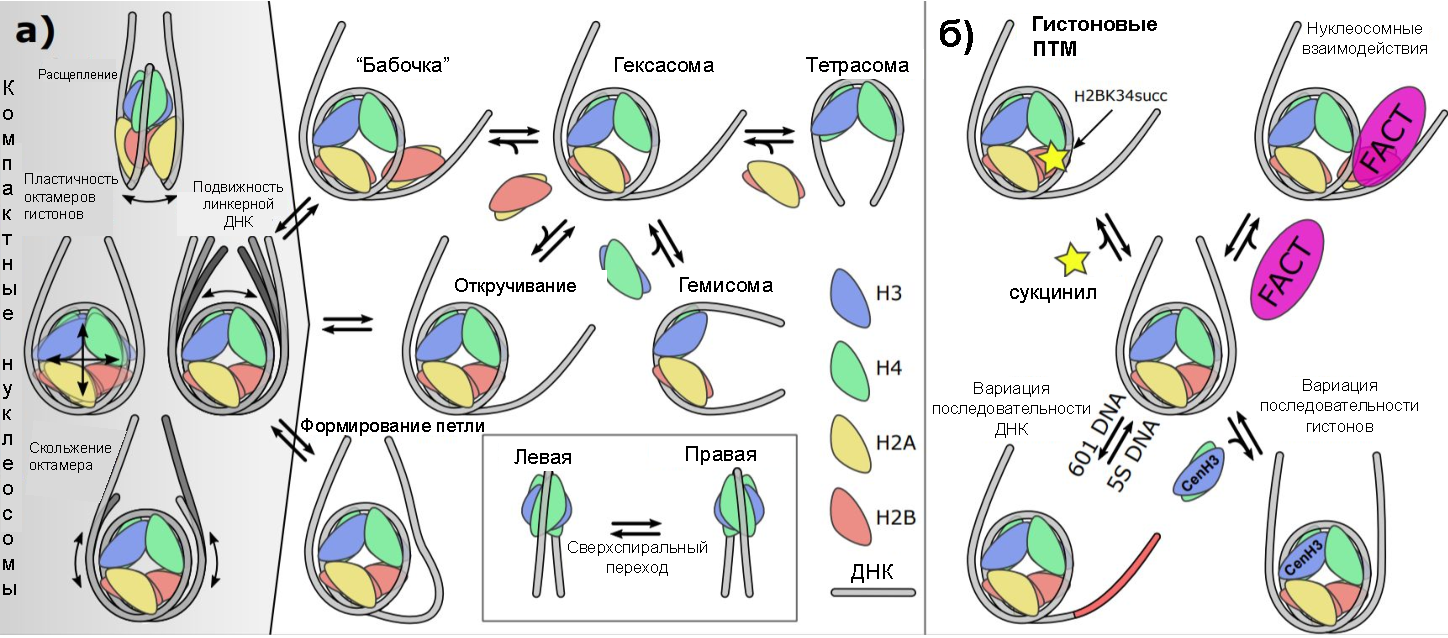
\includegraphics [width=\textwidth]{images/p2/cosb/part2_1_f2.pdf}
    \caption[Моды динамики нуклеосом]{(а) Обзор различных мод динамики нуклеосом. Слева (серая область) показаны режимы, сохраняющие компактность нуклеосомы. Справа показаны моды с большей амплитудой: нуклеосомная ДНК может спонтанно образовывать петли или отворачиваться от гистонов; большие состояния разворачивания ДНК способствуют образованию субнуклеосомных частиц: гексасом, тетрасом, гемисом.
    (б) Примеры факторов, влияющих на структурную динамику нуклеосом. Слева вверху: сукцинилирование H2B по лизину 34 способствует разворачиванию ДНК \cite{jing_site-specific_2018}. Справа вверху: ассоциация с фактором транскрипции FACT изменяет динамику развертывания нуклеосом \cite{valieva_large-scale_2016}. Слева внизу: разные последовательности ДНК имеют разную динамику разворачивания \cite{mauney_local_2018}. Справа внизу: вариант гистона H3 человека CENP-A изменяет подвижность линкерной ДНК \cite{roulland_flexible_2016}.}
    \label{fig:part2_1_f2}
\end{figure}


\subsection{Факторы, влияющие на динамику нуклеосом: недавние примеры}

    Факторы, влияющие на динамику нуклеосом можно разделить на четыре группы (Рис. \ref{fig:part2_1_f2}б): вариации последовательностей гистонов, вариации последовательности ДНК, ПТМ гистонов и различные белки, взаимодействующие с нуклеосомами.

     Белки, взаимодействующие с  нуклеосомами, включают в себя структурные белки хроматина (включая линкер гистона H1 \cite{lyubitelev_structure_2016}), шапероны гистонов, факторы транскрипции (включая пионерские факторы транскрипции \cite{zaret_pioneer_2016}), компоненты репликационного, транскрипционного и эпигенетического аппарата. Они могут влиять на любой из обсуждаемых режимов динамики нуклеосом. Например, гистоновый шаперон FACT обратимо разворачивает нуклеосомную ДНК с обоих концов \cite{valieva_large-scale_2016}, чтобы облегчить обмен димера гистона H2A-H2B \cite{wang_histone_2018}. Гистоновый шаперон Nap-1 является другим примером, он вытесняет димер H2A-H2B из нуклеосомы, и может действовать без необходимости изначального отворачивания ДНК \cite{lee_single-molecule_2017}. Показано, что на раскрытие центромерных нуклеосом влияет взаимодействие с белком CENP-C \cite{falk_cenp-c_2015}. Напротив, ПАРП-1 (многодоменный белок, который управляет обнаружением одно- и двухцепочечных разрывов во время репарации ДНК) значительно увеличивает расстояние между супервитками нуклеосомной ДНК в обратимой манере \cite{sultanov_unfolding_2017}. Линкерные участки ДНК могут притягиваться друг к другу гистоном H1, который снижает их гибкость \cite{bednar_structure_2017}.

    Неструктурированные гистоновые хвосты исторически были основными целями для исследования эффектов различных PTM гистонов на динамику нуклеосом \cite{bowman_post-translational_2015} (Рис. \ref{fig:part2_1_f1}б). По умолчанию считается, что модификации, изменяющие заряд (например, ацетилирование лизина, фосфорилирование серина или отщепление гистонового хвоста), вызывают дестабилизацию нуклеосом за счет снижения не-специфического электростатического притяжения между ДНК и гистонами \cite{fenley_modulation_2018}. Однако существуют свидетельства в пользу того, что более тонкие эффекты также могут иметь значение, такие как изменения вторичной структуры гистоновых хвостов (напр., для H4K16ac \cite{potoyan_regulation_2012}). ПТМ, расположенные на сайтах связывания гистонов с ДНК, могут оказывать более специфические эффекты, нарушая связывание с ДНК соответствующих местах. Например, недавно проанализированное сукцинилирование H2BK34, расположенного в сайте связывания ДНК гистонами на расстоянии $\sim$25 п.н. от точки входа/выхода в нуклеосоме, ингибирует сборку нуклеосом и способствует разворачиванию ДНК \cite{jing_site-specific_2018}. Важность ПТМ гистонов, локализованных в глобулярной части гистонов, и их функциональное значение в настоящее время также широко признаны. Например, H3K56ac облегчает разворачивание нуклеосом и играет важную роль в регуляции сборки нуклеосом \cite{zhang_multisite_2018}. Не изменяющие заряд ПТМ, такие как H3R42me2, также могут способствовать дестабилизации нуклеосом \cite{casadio_h3r42me2a_2013}; последний также использовался микобактериями для изменения эпигенетического ответа хозяина \cite{yaseen_mycobacteria_2015}. ПТМ на границах раздела гистон-гистон могут как нарушать образование октамера \cite{ye_histone_2005}, так и стабилизировать нуклеосомы (например, H4K77ac из-за устранения электростатического отталкивания внутри димера гистона \cite{fenley_modulation_2018}). Сходным образом, H1K85ac ведет к общей стабилизации хроматина и линкерной ДНК за счет увеличения связывания глобулярного домена H1 с коровыми гистонами \cite{li_histone_2018}.

    Нет сомнений в том, что вариация последовательности ДНК может оказывать значительное функциональное воздействие, изменяя вероятность разворачивания ДНК и стабильность нуклеосом. Например, сильно взаимодействующая последовательность ``601'', если ее поместить на нуклеосому, образует полярный барьер для транскрипции \cite{bondarenko_nucleosomes_2006}. Это соответствует известному асимметричному разворачиванию последовательности ``601'' под напряжением \cite{ngo_asymmetric_2015} и в состоянии покоя. Последнее было недавно подтверждено малоугловым рассеянием рентгеновских лучей по сравнению с симметричным разворачиванием, наблюдаемым для 5S рибосомной последовательности \cite{mauney_local_2018}. Динамические эффекты также играют роль во время связывания факторов транскрипции, как первоначально было предложено J. Widom и соавторами \cite{polach_mechanism_1995}. Например, недавняя крио-ЭМ структура нуклеосомы, включающая энхансерную последовательность ALB1 (ALB1 является сайтом связывания для пионерского фактора транскрипции FoxA), аналогична структуре 601-нуклеосомы, но ДНК в области связывания FoxA является более подвижной, способствующей связыванию FoxA \cite{takizawa_cryo-em_2018}. Несмотря на многочисленные усилия, точная взаимосвязь между последовательностью ДНК и ее влиянием на динамику нуклеосом все еще не ясна. По данным некоторых работ присутствие гибких пиримидин-пуриновых динуклеотидов (YR) в сайтах связывания ДНК является важным фактором для позиционирования ДНК и силы связывания (Рис. \ref{fig:part2_1_f1}в) \cite{cui_structure-based_2010,segal_dna_2009}. Однако развитию более общих теоретических моделей в настоящее время препятствует отсутствие достаточно подробных и воспроизводимых экспериментальных наборов данных о связи последовательности ДНК с ее стабильностью на нуклеосоме \cite{eslami-mossallam_nucleosome_2016}. Атомистическое и крупнозернистое компьютерное моделирование может восполнить этот пробел: как недавно показали несколько исследований с использованием моделирования, в зависимости от физических свойств последовательности ДНК, ее транслокация может предпочтительно происходить через винтовой механизм ``распространения дефектов кручения'' или механизм ``повторного захвата петли'' \cite{lequieu_silico_2017,niina_sequence-dependent_2017}.

    Варианты гистонов обеспечивают богатый репертуар вариаций канонической гистоновой последовательности, варьирующийся от всего лишь нескольких аминокислотных различий (например, H3 vs H3.5) до довольно существенных различий, которые могут изменять несколько динамических режимов одновременно (Рис. \ref{fig:part2_1_f1}б). Напр., CENP-A (вариант, критический для образования центромер во время митоза) имеет более короткую спираль $\alpha$N, чем канонический H3. Эта особенность делает линкерную ДНК в CENP-A нуклеосомах более гибкой и влияет на связывание ДНК с гистонами \cite{roulland_flexible_2016}. Кроме того, CENP-A влияет на разворачивание ДНК и способствует образованию петель \cite{stumme-diers_nanoscale_2018}. Известно также, что нуклеосомы CENP-A демонстрируют расщепление половинок нуклеосомы вдоль оси суперспирали \cite{falk_cenp-c_2015}. Варианты с небольшими изменениями канонической гистоновой последовательности также могут быть функционально очень важными: H3.3 важен для пластичности нейронов \cite{maze_critical_2015}, H3.5 для сперматогенеза \cite{urahama_histone_2016}, а H3.Y изменяет регуляцию клеточного цикла \cite{wiedemann_identification_2010}. В последние годы было показано, что эти небольшие вариации последовательности могут влиять на стабильность и динамику нуклеосом. Например, H3.5-специфический остаток лейцина 103 дестабилизирует нуклеосому, что важно для процесса транскрипции в тестикулярных клетках человека \cite{urahama_histone_2016}. Как показано в \cite{kujirai_identification_2017}, в H3.Y метионин 124 способствует стабильной ассоциации тетрамера H3.Y-H4 с ДНК. Другой H3.Y-специфический остаток -- лизин 42 -- играет роль в придании гибкости линкерной ДНК. 
    
    Более того, оказывается, что небольшие вариации между последовательностями канонических гистонов, кодируемых разными копиями генов канонических гистонов у человека, также могут функционально влиять на стабильность нуклеосом. Вариации M51L и K99R в гене гистона HIST1H2AH (изоформа H2A1H) приводят к стабилизации нуклеосом и изменяют пролиферацию клеток \cite{bhattacharya_histone_2017}. Точно так же теперь описаны эффекты небольших вариаций между каноническими последовательностями у разных видов. Специфичный для грибов гистоновый мотив H3 QKK (Рис. \ref{fig:part2_1_f1}в), расположенный на оси диады нуклеосомы, вносит вклад в плохую сборку октамеров в нуклеосомах дрожжей \cite{leung_unique_2016}.


\subsection{Тонкие детали динамики нуклеосом}

    Если распечатать димеры гистонов на 3D-принтере то из можно собрать в октамера подобно конструктору LEGO (см. 3D-печатные модели нуклеосом на \url{https://github.com/intbio/nuclLEGO}). Этот взгляд на нуклеосому как на жесткую модульную структуру теперь уступает место альтернативному взгляду на нуклеосому как на динамическую сущность, где даже небольшие конформационные вариации функционально важны. В поддержку последней точки зрения мы обсудим несколько недавних наблюдений, представленных на рисунке \ref{fig:part2_1_f3}. Во-первых, динамика ДНК внутри нуклеосомы выходит за рамки простого разворачивания и может демонстрировать различные искаженные конформации, включая дефекты кручение и выпячивание ДНК вблизи точки входа/выхода. Такого рода изменения недавно наблюдались как при атомистическом моделировании \cite{shaytan_coupling_2016} (Рис. \ref{fig:part2_1_f3} a), так и на крио-ЭМ картах \cite{bilokapic_histone_2018} (Рис.\ref{fig:part2_1_f3}в). Более того, изменения в конформации ДНК связаны с тонкими изменениями конформации гистоновых белков. Например, как показано в крио-ЭМ, разворачивание 15 пар оснований ДНК с одной стороны октамера гистонов приводит к изменениям конформации гистонов вблизи точек входа / выхода с обеих сторон, а также сопровождается общим небольшим расширением октамера перпендикулярно оси симметрии нуклеосомы \cite{bilokapic_histone_2018}. Более того, определенная связь между перестройками гистонового ядра и конформацией ДНК также наблюдалась для полностью завернутого состояния (Рис.\ref{fig:part2_1_f3}г), было показано, что нуклеосомы могут сокращаться на 8\% вдоль оси диады и расширяться на 5\% в перпендикулярном направлении \cite{bilokapic_structural_2018}.

  Пластичность индивидуальных димеров гистонов также функционально важна. В дополнение к недавно продемонстрированной важности пластичности H3-H4 для ремоделирования нуклеосом \cite{sinha_distortion_2017}, с помощью твердотельного ЯМР было показано, что внутренняя динамика во временных масштабах от наносекунд до миллисекунд присутствует для гистона H4 в нуклеосомах \cite{shi_structure_2018}. Недавнее исследование метил-TROSY ЯМР показало, что мутантные нуклеосомы могут проявлять значительно повышенную динамику внутри гистонов H3-H4 \cite{kitevski-leblanc_investigating_2018}. Помимо H3-H4, пластичность H2A-H2B, по-видимому, также имеет решающее значение для сборки и функционирования нуклеосом. В частности, сборка нуклеосом \textit{in vitro} со сшитыми димерами H2A-H2B происходит только до стадии гексасом \cite{bilokapic_histone_2018}, а это означает, что для сборки требуется определенная гибкость димера. Структура ЯМР  изолированного димера H2A-H2B в растворе, вероятно, отражает эти динамические режимы и демонстрирует повышенную гибкость и беспорядок, в частности, внутри дополнительных спиралей $\alpha$C и $\alpha$N по сравнению со структурой внутри нуклеосомы (Рис.\ref{fig:part2_1_f3}е) \cite{moriwaki_solution_2016}. Динамика H2A-H2B также, вероятно, используется ремоделером SWR1. Он распознает специфически канонические нуклеосомы, содержащие H2A, и заменяет H2A его вариантом H2A.Z. Способность ремоделера SWR1 распознавать и действовать на нуклеосомы H2A на не на H2A.Z недавно была связана с отличием нескольких аминокислот между H2A и H2A.Z. Причем ни одна из этих аминокислот не экспонируется на поверхности нуклеосом \cite{ranjan_h2a_2015}. Поскольку рентгеновские исследования показывают очень похожую структуру нуклеосом H2A и H2A.Z \cite{suto_crystal_2000}, эти открытия подразумевают, что присутствует некая динамическая сигнатура, которая используется для распознавания нуклеосом H2A.
    
    Наконец, тонкая динамика гибких гистоновых хвостов с их способностью взаимодействовать с ДНК и другими белками формирует еще один уровень динамической сложности. Гистоновые хвосты и другие белки хроматина несут положительно заряженные остатки (особенно аргинины \cite{west_electrostatic_2010,dragan_energetics_2003}), которые предпочитают взаимодействовать с малыми бороздками ДНК как участками отрицательного электростатического потенциала (Рис. \ref{fig:part2_1_f3} б). Эти взаимодействия могут, в свою очередь, модулироваться ПТМ гистонов или AT-богатыми последовательности ДНК (что способствует образованию узких малых бороздок \cite{freeman_dna_2014} и может распознаваться некоторыми белками в контексте нуклеосом \cite{xiao_molecular_2017}) (Рис. \ref{fig:part2_1_f1} в). 



\begin{figure} [H]
    \centering
    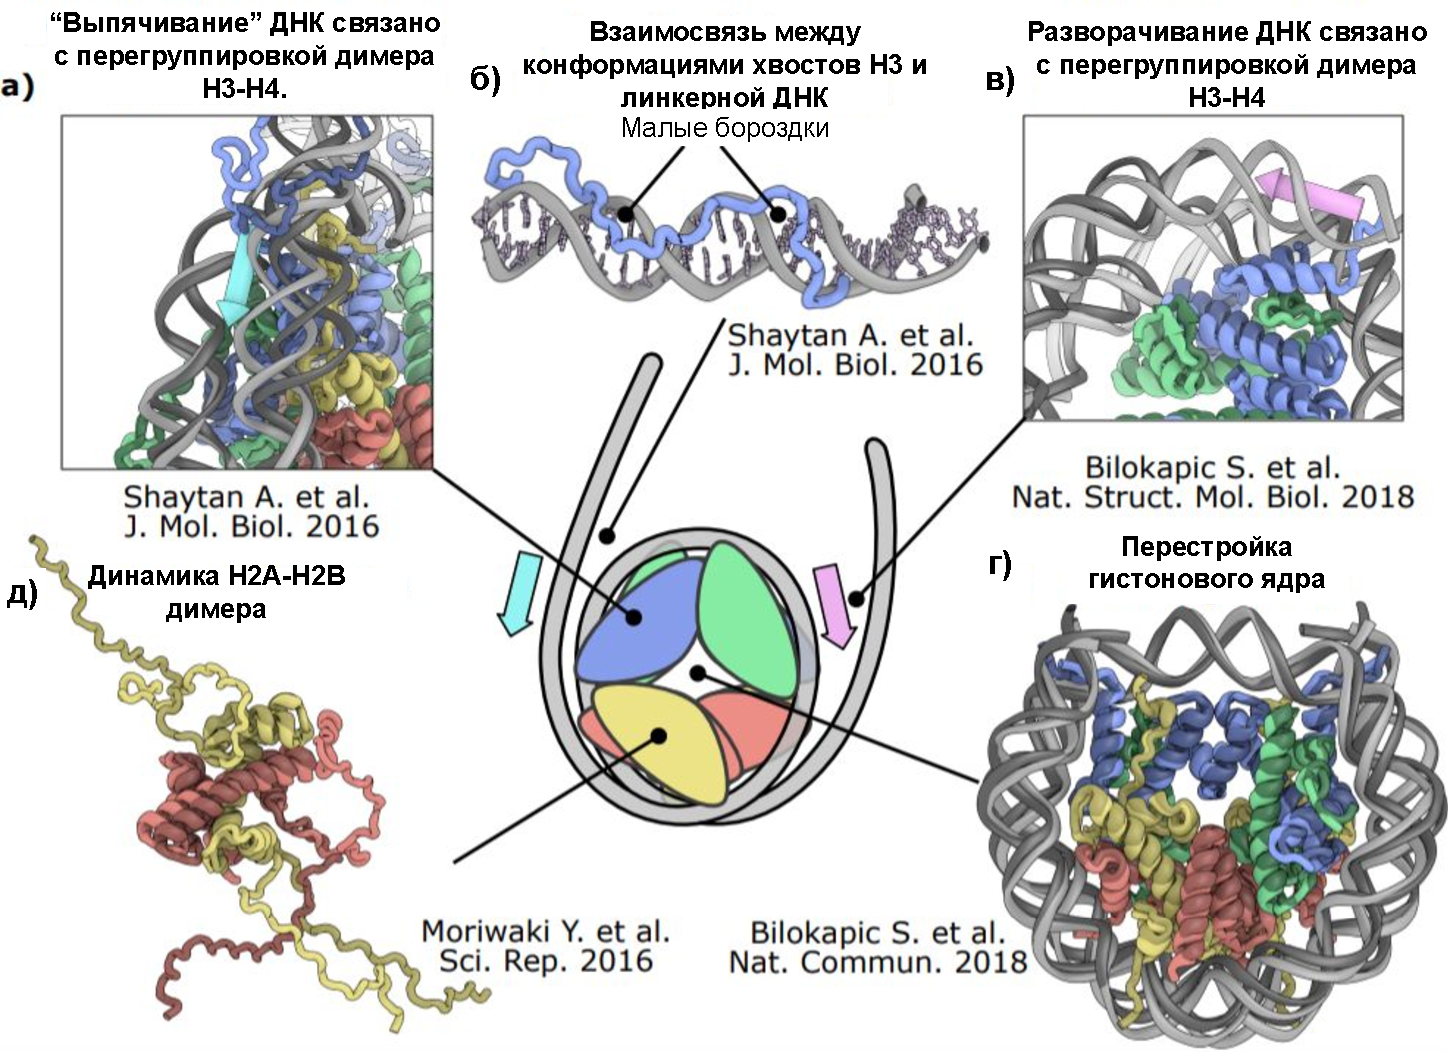
\includegraphics [width=\textwidth]{images/p2/cosb/part2_1_f3.pdf}
    \caption[Тонкие детали динамики нуклеосом]{Динамика ДНК в нуклеосомах тесно связана с динамикой гистонов (a, б, в, г). Цветовая схема соответствует рисунку \ref{fig:part2_1_f1}. Голубые и фиолетовые стрелки на центральной диаграмме и панелях (а) и (в) обозначают одни и те же области входа / выхода ДНК в нуклеосому. (а) Помимо простого разворачивания ДНК, ДНК может проявлять выпуклости возле точек входа / выхода, как это наблюдается в моделировании МД и крио-ЭМ \cite{bilokapic_histone_2018,shaytan_coupling_2016}.  (б) Гистоновый хвост H3 взаимодействует с линкерным сегментом ДНК. Наблюдаются преимущественные взаимодействия с малыми бороздками ДНК \cite{shaytan_coupling_2016}.
    (в) Раскручивание ДНК  сопровождается перестройками в димере гистона H3-H4 \cite{bilokapic_histone_2018}. Кристаллическая структура нуклеосомы показана светлыми цветами. 
    (г) Гистоновый октамер с полностью обернутой ДНК может принимать сжатую конформацию вдоль оси диады (темные цвета) по сравнению с кристаллической структурой по умолчанию (светлые цвета) \cite{bilokapic_structural_2018}. 
    (д) Гибкость димера гистона H2A-H2B, наблюдаемая с помощью ЯМР-исследований в растворе \cite{moriwaki_solution_2016}. Две конформации показаны темным и светлым цветами.}
    \label{fig:part2_1_f3}
\end{figure}
















% COSB - последний

\section{Моделирование нуклеосом с линкерными участками ДНК}
\textit{Данный раздел написан по материалам статей \cite{shaytan_coupling_2016,shaytan_trajectories_2016}, результаты которых основаны в том числе на предыдущих работах \cite{armeev_conformational_2015,armeev_molecular_2015,gribkova_investigation_2017,armeev_nucleosome_2016}.}

%\todo{2S - сюда нужно вставить переведенные текст с картинками materials\/jmb\_2016\/paper.docx, картинки нужно засунуть в гугл Draw (папка p2) - там перевести наложив поверх английского текста русский. Ссылки на литературу уже загружены в зотеро (если вдруг чего-то нет, нужно написать мне). Все заголовки начинать с уровне subsection и далее}

    При формировании нуклеосом октамер гистоновых белков организует около 200 пар оснований ДНК в два суперспиральных витка. Хотя статическая структура коровой частицы нуклеосомы была разрешена, детали динамических взаимодействий между гистонами и ДНК остаются не совсем понятными. Для изучения данного вопроса мы провели длительное равновесное моделирование молекулярной динамики нуклеосом, включая линкерные сегменты ДНК и полноразмерные гистоны, в явном растворителе в атомистическом приближении. Впервые мы смогли идентифицировать и охарактеризовать перестройки в нуклеосомах на микросекундном масштабе времени, изучить связь между конформацией гистоновых хвостов и геометрией ДНК. Мы обнаружили, что определенные конформации гистонового хвоста способствовали выпячиванию ДНК вблизи участков ее входа/выхода в/из нуклеосомы, что приводило к образованию дефектов кручения внутри ДНК. Мы охарактеризовали динамику гистоновых хвостов при их конденсации на нуклеосомальной и линкерной ДНК и показали, что хвосты могут принимать конформационно ограниченные позиции из-за вставки  лизинов и аргининов в малые бороздки ДНК. Потенциально, эти явления влияют на доступность посттрансляционно модифицированных остатков гистонов, которые служат важными сайтами для эпигенетических меток (например, в H3K9, H3K27, H4K16). Предполагается, что взаимодействия гистоновых хвостов с коровой и линкерной ДНК модулируют процессы взаимодействия белков хроматина с гистонами, модификации хвостов и связывания эффекторных белков. В данном разделе мы обсуждаем влияние наблюдаемых явлений на функцию нуклеосом и сравниваем наши результаты с различными экспериментальными исследованиями.

\subsection{Введение}
    Нуклеосомы - это элементарные единицы компактизации хроматина в геномах эукариот, расположенные через каждые 200 $\pm$ 40 п.н. вдоль ДНК \cite{mcghee_nucleosome_1980}. Основным источником информации об атомистической структуре нуклеосомы являются рентгеновские исследования коровых частиц нуклеосом (NCP) (см. обзор \cite{dechassa_nucleosomes_2011}), которые неизменно разрешают очень похожие структуры гистонов и ДНК независимо от вариантов последовательности гистонов, мутаций, посттрансляционные модификации, последовательности ДНК или присутствия белков, связывающих нуклеосомы, пептидов или химических агентов. Например, суперпозиция различных структур нуклеосом с использованием алгоритма VAST+ \cite{madej_mmdb_2014} показала очень небольшие вариации в среднеквадратичном отклонении (RMSD) около 1 \AA для выровненных глобулярных частей гистоновых областей. Консенсусная структура NCP формируется путем наматывания $\sim$ 145-147 п.н. коровой ДНК в $\sim$ 1,7 левых сверхспиральных витка вокруг октамера, состоящего из четырех типов коровых гистонов (H3, H4, H2A, H2B) \cite{marino-ramirez_histone_2011}. Структура NCP характеризуется наличием диадной оси - оси псведосимметрии второго порядка, сильно изогнутой структурой ДНК \cite{tolstorukov_novel_2007} и высоким положительным зарядом октамера гистонов \cite{fenley_charge_2010}. Кроме того, он включает большое количество молекул воды, проникающих в структуру нуклеосомы \cite{davey_solvent_2002}, а также длинные гистоновые хвосты, выступающие из ядра нуклеосомы и обеспечивающие множество сайтов для посттрансляционных модификаций (ПТМ).

    С другой стороны, решающая роль нуклеосом в функционировании хроматина (включая тонкую регуляцию экспрессии генов, репликацию ДНК, репарацию и наследование, опосредованные эпигенетическими механизмами \cite{henikoff_nucleosome_2008,petty_balancing_2013}) зависит от их динамической природы и конформационных переходов. Действительно, многие биофизические (FRET, эксперименты с одномолекулярными пинцетами и другие, рассмотренные в \cite{choy_structural_2012}) и биохимические эксперименты (анализ связывания факторов транскрипции \cite{li_rapid_2005}, химическая сшивка \cite{lee_n-terminal_1997}, анализ методом ChIP-exo  \cite{rhee_subnucleosomal_2014}) предполагают, что нуклеосомы демонстрируют существенный конформационный полиморфизм как на локальном (конформация ДНК и гистоновых хвостов внутри нуклеосомы), так и на глобальном (потеря гистонов, субнуклеосомные частицы и т. д.) масштабах, которые, в свою очередь, могут быть результатом равновесных тепловых флуктуаций или могут быть активно индуцированы внешними силами внутри клетки.
    
    Были предложены различные функционально значимые моды динамики нуклеосом, которые включают дыхание/разворачивание/раскрытие ДНК, расщепление нуклеосом \cite{zlatanova_nucleosome_2009}, а также скольжение нуклеосом \cite{mueller-planitz_nucleosome_2013}, раскрытие или потерю димера H2A-H2B \cite{shaytan_nucleosome_2015}. В то же время, различные конформационные перестройки гистоновых хвостов необходимы для внутри- и межнуклеосомных взаимодействий \cite{pepenella_intra-_2014}, для множественных взаимодействий с ремоделерами хроматина \cite{hwang_histone_2014,racki_histone_2014}, гетерохроматиновыми белками \cite{wang_heterochromatin_2013} и со многими эффекторными белками, которые содержат домены, связывающие модификации гистонов \cite{rando_combinatorial_2012}. Тем не менее, взгляду на нуклеосомы как на динамические объекты \cite{zlatanova_nucleosome_2009} все еще не хватает понимания деталей на атомистическом уровне.

    Чтобы попытаться сгладить этот очевидный пробел в нашем понимании динамики и функций нуклеосом, уже были предприняты значительные усилия в области моделирования, включая моделирование молекулярной динамики (МД) на атомистическом уровне \cite{biswas_atomistic_2013} и моделирование в крупнозернистом приближении \cite{arya_role_2006,collepardo-guevara_chromatin_2014}. Однако из-за значительного размера нуклеосомы по стандартам атомистического моделирования и чрезвычайно долгих временных масштабов ее функциональной динамики в предыдущих исследованиях приходилось прибегать либо к крупнозернистому моделированию без атомистических деталей, либо к полностью атомному моделированию без явных молекул растворителя \cite{erler_role_2014}. Полноатомное моделирование проводилось на временах не превышающих нескольких сотен наносекунд \cite{materese_counterion_2009,ruscio_computational_2006}. Однако мы знаем, что изменения в атомных взаимодействиях могут иметь глубокие функциональные последствия для нуклеосом. Например, посттрансляционные модификации могут изменять внутри- и межнуклеосомные взаимодействия или обеспечивать множественные сайты связывания для так называемых эффекторных белков \cite{ruthenburg_multivalent_2007}, даже однократное ацетилирование H4K16 может запускать разворачивание хроматиновых волокон \cite{dorigo_chromatin_2003,norouzi_topological_2015-1}.

    В работе, изложенной в данном разделе, концептуальный прогресс состоит в том, чтобы использовать наиболее надежный подход моделирования методом МД с явным  растворителем для всех атомов  и расширить этот подход на значительно более длительную микросекундную шкалу времени. Микросекундное моделирование, а также модели нуклеосом с реалистичными сегментами ДНК-линкера и многочисленные сравнительные модели позволили нам получить представление о функционально значимых перестройках в нуклеосомах, включая связь между конформациями гистоновых хвостов и геометрией ДНК. Хотя многие функционально релевантные движения могут происходить в гораздо более длительных временных масштабах \cite{choy_structural_2012}, несколько недавних исследований ЯМР показали, что гистоновые хвосты демонстрируют субмикросекундную динамику, что дает возможность сравнить наши расчетные результаты с экспериментальными данными \cite{kato_characterization_2009,zhou_histone_2012,gao_histone_2013}.

    В этом исследовании мы обнаружили, что определенные конформации гистонового хвоста способствуют выпячиванию ДНК возле мест входа/выхода ДНК в нуклеосоме, образованию дефектов кручения внутри ДНК и перестройке взаимодействий гистонов с ДНК в нуклеосомном коре. Мы охарактеризовали динамику гистоновых хвостов при их конденсации на коровой и линкерной ДНК на атомистическом уровне и показали, что они могут принимать конформационно ограниченные положения, сопровождаемые вставкой определенных ``закрепляющих'' лизинов и аргининов в малые бороздки ДНК. Мы предполагаем, что эти процессы влияют на доступность посттрансляционно модифицированных остатков гистонов, которые служат важными эпигенетическими метками (например, H3K9, H3K27, H4K16), а взаимодействия с коровой и особенно линкерной ДНК (для хвоста H3) могут модулировать доступность различных сайтов на гистоновых хвостах для связывания эффекторными белками.

\subsection{Результаты}

\subsubsection{Обзор исследованных моделей}
В нашем исследовании мы использовали несколько систем для моделирования, в том числе специально сконструированную полную нуклеосомную систему с линкерными сегментами ДНК по 20 п.н., фланкирующих коровую частицу с каждой стороны (модель FN) (Рис. \ref{fig:p2_2_f1}а), минималистичную модель коровой частицы с усеченными гистоновыми хвостами (NCPm модель) и набор вспомогательных систем с различными условиями моделирования (подробности см. в таблице \ref{tbl:p2:jmb_t1}). Ниже мы в основном сосредотачиваемся на результатах, полученных для полной нуклеосомной системы, для которой были выполнены обширные микросекундные расчеты. Мы допускаем, что динамика нуклеосом происходит в нескольких временных масштабах, а функционально значимые конформационные переходы часто превышают масштаб времени в одну микросекунду. Наше моделирование ограничивалось исследованием конформационных ансамблей вокруг определенных локальных квазиравновесных состояний в микросекундной шкале времени. Поэтому, интерпретируя результаты нашего моделирования, проверяли наши выводы, выполняя несколько вспомогательных расчетов. При обсуждении результатов ниже мы ссылаемся на ключевые структурные элементы гистоновых последовательностей и нуклеосом, как показано на рисунке \ref{fig:p2_2_f2} (см. Также раздел ``Название элементов структуры нуклеосом'' ниже).


\begin{table}[p]
\caption{Исследованные в моделировании системы и их параметры}
	\label{tbl:p2:jmb_t1}	
	\begin{tabularx}{\textwidth} { 
  | >{\raggedright\arraybackslash}X 
  | >{\centering\arraybackslash}X 
  | >{\raggedleft\arraybackslash}X 
  | >{\raggedleft\arraybackslash}X 
  | >{\raggedleft\arraybackslash}X 
  | >{\raggedleft\arraybackslash}X |}
  \hline
Название & Описание & Количество атомов, тыс. & Эффект. концентрация соли, мМ & Размер ячейки, \AA & Время моделирования, нс\\
	\hline

FN & Система с линкерной ДНК и гистоновыми хвостами & 366,8 & $\sim$185 & 162х197х113 & 1000 \\
\hline
FN1M & То же, что и не FN, но в высокой концентрации соли & 366,8 & $\sim$1100 & 161х196х112 & 1000 \\
\hline
FNbb & То же, что и не FN, но в большей ячейке & 3200 & $\sim$160 & 322х358х274 & 1000 \\
\hline
FNnt & То же, что и не FN, но с ацетильными и N-метил группами на концах гистонов& 366,8 & $\sim$185 & 162х197х113 & 1000 \\
\hline
NCPm & Cистема, без линкерной ДНК и хвостов гистонов & 310,3 & $\sim$200 & 145х141х101 & 1000 \\
\hline

\end{tabularx}
	 
\end{table}

\begin{figure} [H]
    \centering
    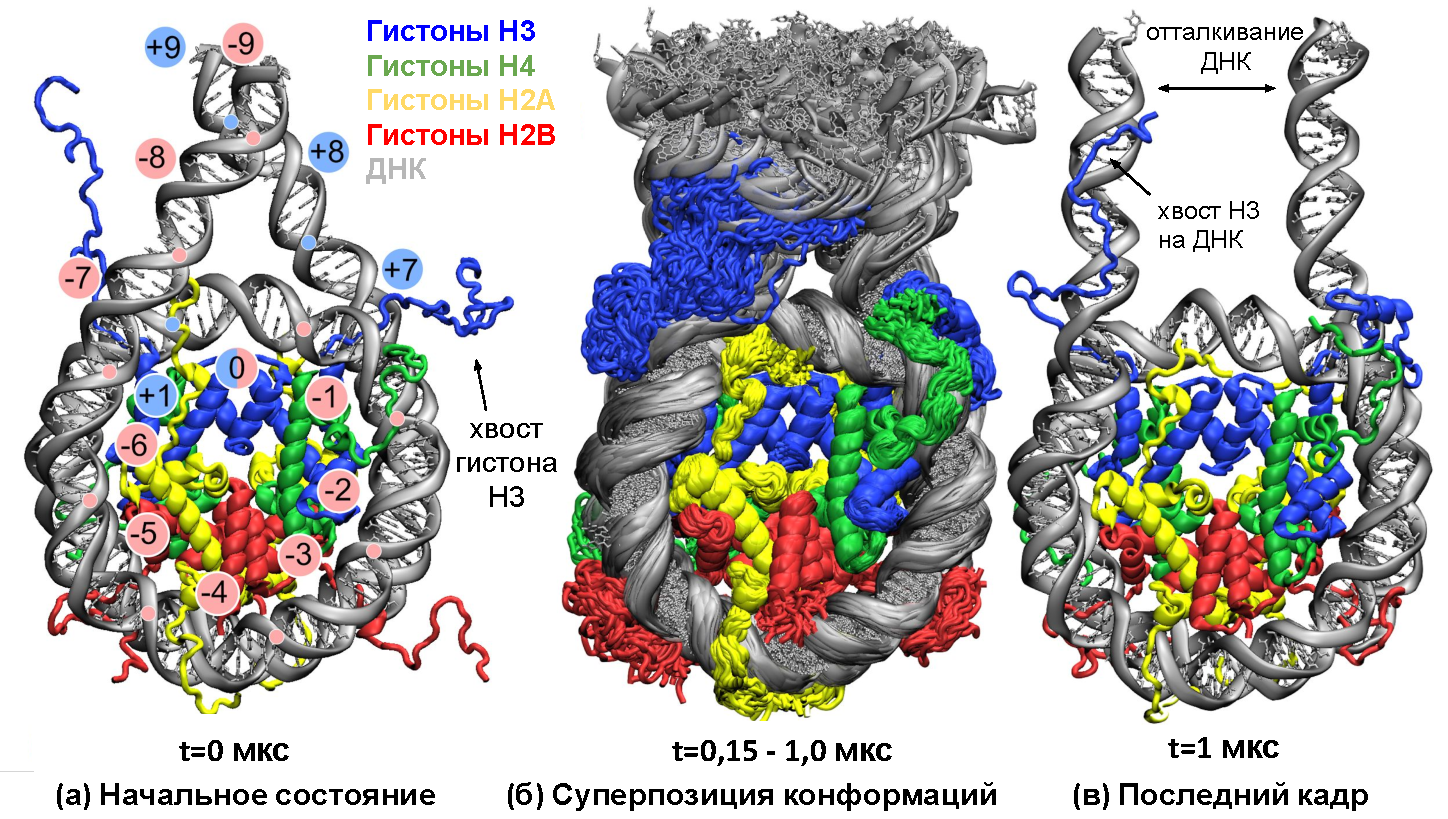
\includegraphics[width=\textwidth]{images/p2/jmb/part2_2_f1.pdf}
    \caption[Обзор структуры и динамики модели полной нуклеосомы (FN)]{Обзор структуры и динамики модели полной нуклеосомы (FN): (a) Исходная структура модели FN, (б) наложенные конформации из последних 75 \% кадров расчетной траектории, (в) последний кадр после 1 мкс, обратите внимание на различные формы N-концевых хвостов H3 с обеих сторон.}
    \label{fig:p2_2_f1}
\end{figure}

\begin{figure} [H]
    \centering
    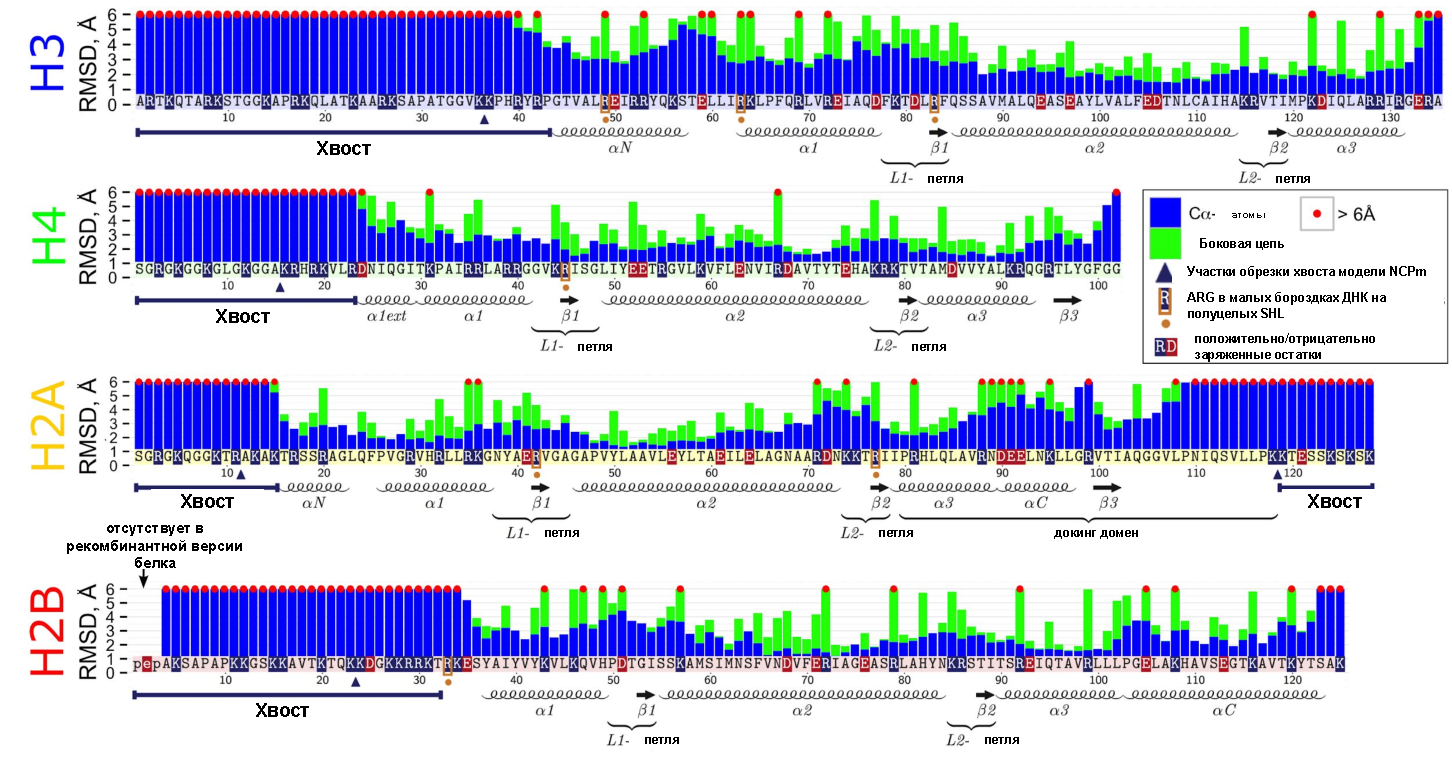
\includegraphics[width=\textwidth]{images/p2/jmb/part2_2_f2.pdf}
    \caption[Максимальные наблюдаемые среднеквадратичные отклонения отдельных аминокислот гистонов 
    в МД моделировании]{Максимальные наблюдаемые среднеквадратичные отклонения отдельных 
    аминокислот (C$\alpha$-атомы - синие столбцы, атомы боковой цепи - зеленые столбцы) во время
     моделирования относительно их положения в исходной рентгеновской структуре. 
     Значения, превышающие 6\AA, усекаются при этом значении и отмечаются красной точкой над столбцом.
      Аннотации структурных элементов гистонов приведены под столбиками.}
    \label{fig:p2_2_f2}
\end{figure}



\subsubsection{Конформационная стабильность и пластичность гистонов и ДНК}

    В соответствии с предыдущими экспериментальными исследованиями, наше моделирование подтвердило общую стабильность ядра нуклеосомы в отношении диссоциации компонентов нуклеосомы или крупномасштабного развертывания ДНК (см. Обзор динамики на рисунке \ref{fig:p2_2_f1}). В целом, RMSD центральной области гистонов оставалось в среднем в пределах 1,5\AA от кристаллографических положений для всех изученных моделей. Это было верно даже для минималистичной системы NCPm с усеченными гистоновыми хвостами. Таким образом, предполагается, что нуклеосомы имеют достаточный запас стабильности в отношении усечения гистоновых хвостов на микросекундных временах. Однако подробный анализ конформационной динамики, представленный ниже, предоставил новое понимание конформационной гибкости нуклеосом и выявил конформационные перестройки внутри гистонового ядра, гистоновых хвостов, ядра ДНК и линкерных областей, которые происходят в микросекундной шкале времени.

    Чтобы предоставить подробную картину динамики гистонов, мы изобразили максимальные отклонения позиций атомов, наблюдаемые в ходе динамики, от положений в кристаллической структуре (Рис. \ref{fig:p2_2_f2}). Как можно видеть на рисунке \ref{fig:p2_2_f2}, относительно большие конформационные изменения более чем на 6\AA наблюдались для атомов остова всех хвостов гистонов, даже некоторые части гистоновых фолдов демонстрируют высокое RMSD. Хотя, как показывает анализ кристаллических структур, докинг домен H2A (docking domain) образует тесные контакты с тетрамером $(H3-H4)_2$ \cite{suto_crystal_2000}, мы продемонстрировали существенные конформационные изменения для С-концевой части этого домена относительно исходной кристаллической структуры. Конформационные флуктуации остова белковой цепи часто сопровождались переориентацией боковых цепей аминокислотных остатков. Например, изменения в $\alpha$C-спирали докинг-домена сопровождались временным образованием новых солевых мостиков между H2A R88 и R99, фланкирующими эту спираль, и H3 E105, D106. Наблюдаемая пластичность докинг-домена будет влиять на его функции в качестве партнера по связыванию белков хроматина. В частности, недавно было показано, что шаперон ANP32E может быть ответственным за встраивание гистона H2A.Z в нуклеосому. ANP32E может связываться с $\alpha$C-спиральной областью докинг-домена H2A.Z \cite{obri_anp32e_2014}, которая в нуклеосоме структурно очень похожа на каноническую $\alpha$C-спираль H2A. Связывание гистона с ANP32E стерически несовместимо с полной структурой нуклеосомы и может запускать разборку и вытеснение нуклеосом, когда гибкая область ANP32E вставляется в кор нуклеосомы. Последний процесс не очень хорошо изучен, однако повышенная конформационная гибкость в этой области, наблюдаемая в нашем исследовании, указывает на возможные механизмы этого процесса. Интересно, что Biswas et al. в более ранних работах по МД моделированию нуклеосом показали потенциальную связь между усечением гистоновых хвостов H3 и конформациями боковых цепей H2A R81 и R88 \cite{biswas_role_2011}. Визуальное исследование траекторий динамики наших систем показывает, что, хотя боковая цепь H2A R88 очень гибкая в микросекундном масштабе времени, боковая цепь H2A R81 в основном заблокирована в своей кристаллографической ориентации и иногда перескакивает в положение, направленное в сторону от октамера гистонов. В последнем положении боковая цепь может находиться сотни наносекунд.

    Кроме того, значительные смещения остова полипептидной цепи (более 3\AA) и боковых цепей (более 6\AA) наблюдались в центральных областях других гистонов, включая H3 $\alpha$N-спираль, H3 $\alpha$1-спираль, сайт связывания L1-L2 димера H2A-H2B и H2B $\alpha$C-спираль) (Рис. \ref{fig:p2_2_f2}). Как уже упоминалось, даже если остов белка не демонстрирует больших отклонений от кристаллографических положений, все же могут происходить значительные изменения конформеров боковых цепей. Фактически, все аминокислоты, кроме одной, с наблюдаемой переориентацией боковой цепи более 6\AA, принадлежали заряженным остаткам. Эти переориентации часто включают разрушение и образование новых солевых мостиков внутри гистонового ядра. Изменения в модели NCPm показали аналогичные закономерности.


    Анализ конформационной динамики коровой и линкерной ДНК показал, что ДНК оставалась в среднем в пределах 4\AA (5 \AA для модели NCPm) от своих кристаллографических положений, измеренных с помощью RMSD атомов N1 и N9 азотистых оснований. Кроме того, фосфатный остов ДНК характеризуется периодическим профилем средних флуктуации (RMSF): участки остова ДНК, контактирующие с гистонами, проявляли значительно меньшие колебания по сравнению с теми, которые были обращены в раствор. С другой стороны, линкерные сегменты ДНК в нашем моделировании явно демонстрировали гораздо более сильные колебания, чем коровые участки ДНК (Рис. \ref{fig:p2_2_f1}б,в), что согласуется с известными данными \cite{pachov_structure_2011}. Глобальная конформация ДНК была дополнительно изучена с помощью 2D-проекций многоугольников, соединяющих центры пар оснований ДНК в нуклеосомной суперспиральной системе отсчета (см. Рис. \ref{fig:p2_2_f3}). Позиционные колебания линкерных сегментов ДНК охватывают частично перекрывающиеся конусообразные области в пространстве с угловым размахом около $\pm$45 градусов в обеих проекциях. Никаких существенных корреляций в позиционных колебаниях линкеров ДНК обнаружено не было. Средние положения, принятые для линкерных цепей ДНК в MD, были дальше друг от друга по сравнению с их исходными положениями, которые соответствовали прямому продолжению концов коровой ДНК (Рис. \ref{fig:p2_2_f3}а). Моделирование той же системы, но в солевом растворе с высоким содержанием 1 М (система FN1M) ясно показало, что два линкера ДНК приближаются друг к другу и даже большую часть времени взаимодействуют своими концами. Предполагаем, что скрининг электростатических взаимодействий значительно повлиял на угол входа/выхода ДНК. Интересно, что более ранние экспериментальные измерения расстояний между линкерами с помощью FRET показали, что расстояние монотонно уменьшается с увеличением концентрации соли \cite{toth_chromatin_2006}.

    Первостепенным вопросом динамики нуклеосом является амплитуда, временная шкала и механизмы отворачивания/дыхания ДНК, разворачивания или открытия поверхности октамера гистонов, что, как полагают, имеет решающее значение для доступности ДНК и связывания факторов транскрипции \cite{li_rapid_2005,mirny_nucleosome-mediated_2010}. К сожалению, на сегодняшний день нет полной картины, поскольку разные экспериментальные установки, интерпретация и терминология часто поддерживают разные взгляды на эту проблему \cite{choy_structural_2012,zlatanova_nucleosome_2009}. В этом исследовании мы не наблюдали крупномасштабного разворачивания или раскрытия коровой ДНК ни в системах FN, ни в системах NCPm. Такое разворачивание, если оно произойдет, обнажит достаточно частей ДНК для распознавания факторами транскрипции. Наши результаты согласуются с экспериментальными оценками временных масштабов событий разворачивания, которые лежат в субсекундном диапазоне \cite{li_rapid_2005,tomschik_nucleosome_2009}. Однако, если мы рассмотрим более умеренные колебания концов коровой ДНК вместе с линкерной ДНК (часто называемые ``дыханием ДНК''), такие процессы могут происходить в более коротких временных масштабах \cite{gansen_nucleosome_2009}. Например, недавние измерения FRET расстояний между двумя красителями, расположенными симметрично на обоих сегментах линкерной ДНК на расстоянии 5 п.н. от сайтов входа / выхода ДНК, показали две разные конформации с характерными расстояниями между двумя красителями $\sim$4,5 нм и $\sim$6,5 нм (амплитуда около 2 нм), в предположении  модели с двумя состояниями \cite{nurse_clipping_2013}. В нашем моделировании расстояние между центрами пар оснований соответствующих позиций линкеров ДНК варьировалось от 4,5 нм до 6,8 нм (см. Рис. \ref{fig:p2_2_f3}) (со средним значением 5,6 нм и RMSF 0,4 нм), показывая, что эти диапазоны расстояний находятся в пределах досягаемости быстрых субмикросекундных колебаний. Кроме того, мы наблюдали асимметрию в средних конформациях ДНК двух линкеров, а также в их отклонениях от исходной кристаллической структуры (обозначенной стрелками на рисунке \ref{fig:p2_2_f3}). Интересно, что если мы предположим, что наблюдаемые асимметрии соответствуют двум различным стабильным конформационным состояниям ДНК в нуклеосоме, переход между этими состояниями может уже объяснить изменение положения ДНК в  0,5 нм на расстоянии 5 п.н. от входа/выхода. Однако мы признаем, что методология для точного сравнения различных конформационных переходов, наблюдаемых при моделировании, и результатов измерений FRET все еще требует разработки и проверки: как недавно было отмечено Ленцем и др., флуктуация формы ДНК в нуклеосоме может размывать сигналы FRET от промежуточных конформационных состояний ДНК в нуклеосоме \cite{lenz_influence_2015}.

    В следующих разделах мы продемонстрируем, что эти конформационные асимметрии ДНК следствие асимметричной конденсацией гистоновых хвостов. Хотя мы находим, что время, необходимое для переключения между различными конформациями гистоновых хвостов, явно превышает микросекундную шкалу времени, мы предполагаем, что динамика ДНК в микросекундной шкале времени определяется взаимодействиями между гистоновыми хвостами и ДНК, которые, в свою очередь, могут влиять на конформацию ДНК на гораздо более длительных временах.
    %корявый перевод получился последнего абзаца, не понимаю как на русском правильно написать

\begin{figure} [H]
    \centering
    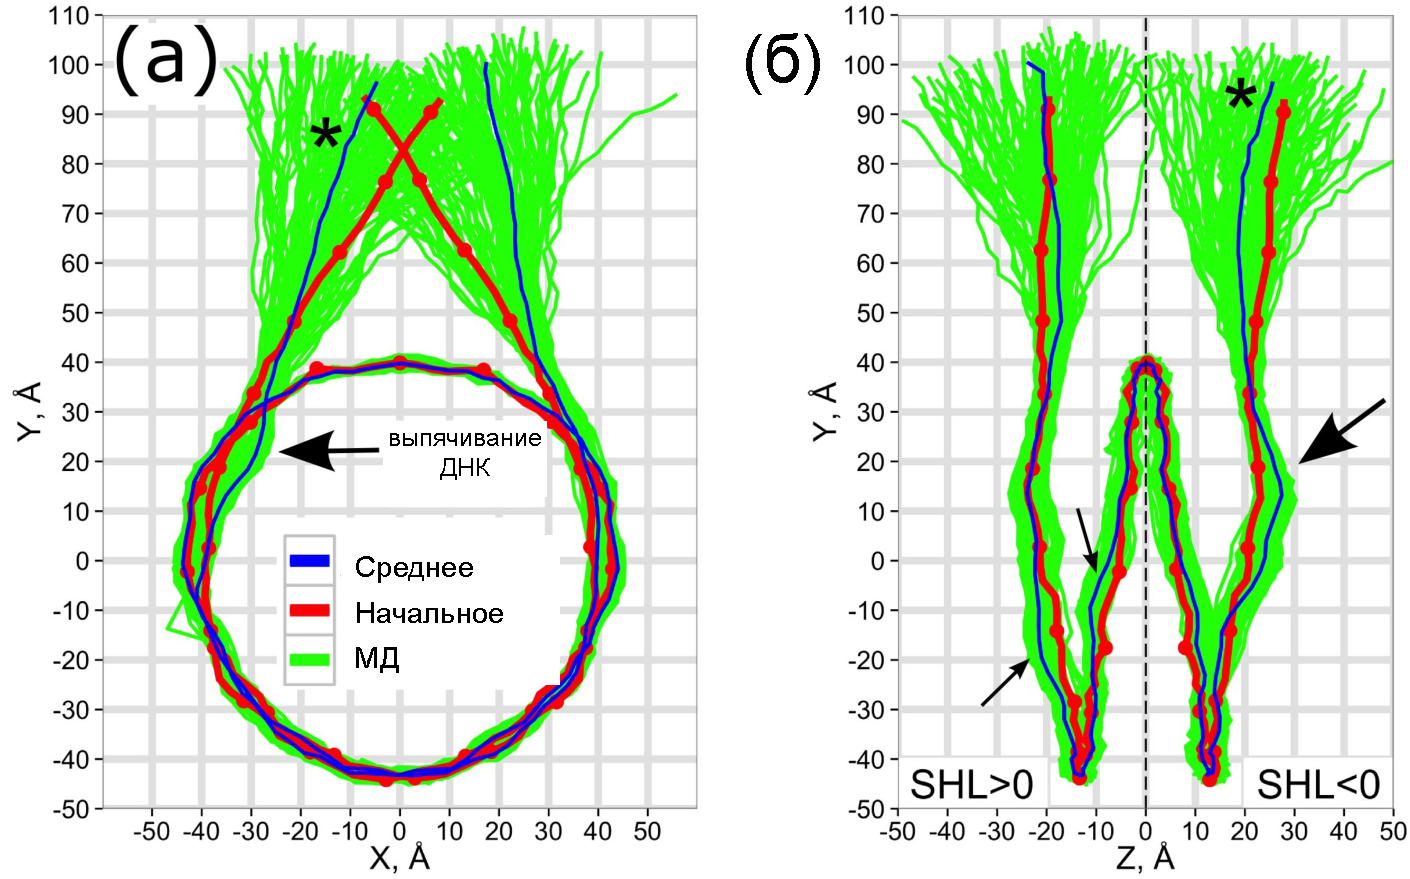
\includegraphics[width=\textwidth]{images/p2/jmb/part2_2_f3.pdf}
    \caption[Конформационный ансамбль ДНК в нуклеосоме]{Конформационный ансамбль ДНК в нуклеосоме, (а) - передняя и (б) - боковые проекции. Красными точками отмечены целые и полуцелые значения суперспирального положения (SHL) вдоль исходной конформации, звездочкой отмечен один линкерный сегмент ДНК на обоих рисунках. Стрелки указывают максимальные отклонения между исходной и средней конформациями в МД.}
    \label{fig:p2_2_f3}
\end{figure}

\subsubsection{Быстрая конденсация гистоновых хвостов на коровой и линкерной ДНК}
    Положительно заряженные гистоновые хвосты были тщательно изучены как экспериментально, так и с помощью методов моделирования. Известно, что межнуклеосомные взаимодействия опосредуются хвостами и играют важную роль в уплотнении хроматина. В этой работе мы охарактеризовали динамику взаимодействий между гистонами и ДНК на атомном уровне и обнаружили, что в среднем 60\% всех контактов были обеспечены взаимодействиями ДНК с участками гистонового хвоста. Хвосты гистонов, которые в исходной модели выступали в объем растворителя (в основном хвосты H3, Рис. \ref{fig:p2_2_f1}а), быстро адсорбировались на ДНК в течение первых 20 нс моделирования. От 50 до 90\% всех аминокислот в этих хвостовых областях имели прямые или опосредованные водой взаимодействия с коровой или линкерной ДНК в течение 1 мкс моделирования (Рис. \ref{fig:p2_2_f4}). Какого-либо существенного скопления контактов к началу или концу хвостов мы не наблюдали. Предыдущие полноатомные МД расчеты нуклеосомных частиц также указали на значительную ассоциацию гистоновых хвостов с коровой ДНК на временном масштабе 100 нс \cite{erler_role_2014,biswas_role_2011,roccatano_structural_2007}. Однако были высказаны определенные опасения по поводу коротких временных масштабов моделирования, а также артефактов, возникающих из-за периодических граничных условий и решеточных методов суммирования электростатических взаимодействий. Чтобы решить последнюю проблему, мы выполнили моделирование на протяжении 80 нс в большой ячейке (система FNbb), размер которой должен минимизировать потенциальные неблагоприятные эффекты периодических граничных условий. Моделирование FNbb подтвердило предпочтительную ассоциацию гистоновых хвостов с ДНК и быструю конденсацию длинных N-концевых хвостов H3. Таким образом, мы снимаем ранее высказанные опасения и показываем, что конденсация гистонового хвоста не является артефактом конкретных методов, используемых в МД-моделировании.

    Несколько исследований малоуглового рассеяния рентгеновских лучей (SAXS) касались вопроса о том, выступают ли гистоновые хвосты из ядра нуклеосомы в раствор или связаны с ДНК с физиологической ионной силой. Сообщалось о значительном увеличении максимального диаметра нуклеосом при повышении концентрации одновалентной соли с 10 мМ до физиологических концентраций и выше \cite{mangenot_salt-induced_2002}. Этот результат был приписан процессу диссоциации гистоновых хвостов от кора нуклеосомы. Однако Ян и др. \cite{yang_biophysical_2011} указали, что сопоставимое увеличение диаметра можно объяснить конформационными изменениями нуклеосом, включая разворачивание ДНК. Наши результаты подтверждают модель, в которой гистоновые хвосты прикреплены к коровой или линкерной ДНК большую часть времени в этой временной шкале. Если по какой-то причине хвосты оторвались, характерное время их присоединения должно составить около нескольких десятков наносекунд, о чем свидетельствует их быстрая конденсация (Рис. \ref{fig:p2_2_f4}). Наши теоретические оценки радиусов гирации предполагают, что и гистоновые хвосты, и линкерная ДНК вносят вклад в увеличение радиусов гирации.

    Чтобы дополнительно выяснить влияние концентрации соли на поведение хвоста, мы выполнили моделирование при чрезвычайно высокой концентрации соли 1M (модель FN1M). Хотя известно, что октамерная форма нуклеосом нестабильна при такой концентрации соли \cite{wilhelm_reconstitution_1978}, мы не наблюдали никакой разборки нуклеосом, что позволяет предположить, что это происходит во временном масштабе, намного превышающем микросекунду. В то время, как текущее силовое поле может несколько переоценивать натрий-фосфатные взаимодействия при высоких концентрациях соли \cite{yoo_improved_2012}, оно не должно препятствовать отсоединению хвостов от ДНК. Тем не менее, это позволяет нам исследовать эффекты повышенной концентрации соли на гистоновые хвосты и линкерную ДНК, в то время как ядро нуклеосомы все еще остается в компактном состоянии. Интересно, что хотя хвостам (особенно хвосту H3) потребовалось несколько больше времени (70 нс по сравнению с 20 нс при концентрации соли 150 мМ), чтобы установить контакты с ДНК из их исходной конформации, гистоновые хвосты все еще конденсируются на ДНК, несмотря на значительное усиление скрининга электростатических взаимодействий, вызванного высокой концентрацией соли. Этот факт можно рассматривать как еще одно свидетельство, подтверждающее модель тесных взаимодействий между гистоновыми хвостами и ДНК в нуклеосомах, по крайней мере, когда кор нуклеосомы находится в компактно собранном состоянии.

    В литературе ведутся дискуссии о конденсированных и декноденсированных состояниях гистоновых хвостов в нуклеосомах, и, по нашему мнению, основные физические принципы поддерживают последнюю точку зрения. Как обсуждалось в \cite{iwaki_how_2007,korolev_physicochemical_2007}, достаточно длинные олигокатионы имеют тенденцию почти полностью ассоциироваться с высоко заряженной ДНК из-за увеличения свободной энергии при высвобождении конденсированных небольших одновалентных ионов.

    Комбинированный ансамбль конформаций гистоновых хвостов, отобранных в различных моделях, показал широкий диапазон участков ДНК, доступных для взаимодействия с гистоновыми хвостами (Рис. \ref{fig:p2_2_f5}). Например, было показано, что линкерный ДНК-сегмент длиной 20 п.н. полностью доступен для взаимодействий с N-концевым хвостом H3 и частично доступен для взаимодействий с C-концевым хвостом H2A вблизи точки входа / выхода ДНК. В моделях FN и FNnt один N-концевой хвост H3 оставался вытянутым и стабильно связанным с ближайшим линкерным сегментом ДНК (Рис. \ref{fig:p2_2_f1}в и \ref{fig:p2_2_f6}a), в то время как другой хвост образовывал $\alpha$-спираль возле точки входа / выхода ДНК (H3 21-28) или находился между супервитками ДНК (Рис. \ref{fig:p2_2_f6}д, \ref{fig:p2_2_f6}е). Этот наблюдаемый полиморфизм конформаций хвоста H3 перекликается с утверждениями из различных экспериментальных исследований. Связывание хвостов H3 с линкерной ДНК недавно было подтверждено в исследовании ChIP-exo в масштабе генома \cite{rhee_subnucleosomal_2014}. С другой стороны, исследования ЯМР и дейтеро-водородного обмена указывают на то, что в нуклеосомных массивах хвосты H3 могут образовывать стабильные компактные структуры \cite{kato_characterization_2009}. Возможность для H3-хвоста конденсироваться на линкерной ДНК предполагает также его роль в частичной нейтрализации линкерной ДНК и конкурентном связывании с другими белками, взаимодействующими с линкерной ДНК (такими как гистон H1 или определенные комплексы ремоделирования нуклеосом), что важно для понимания функционирования хроматина, учитывая очень высокие концентрации нуклеосом в ядре (> 200 мг/мл) \cite{dehghani_organization_2005}.






\begin{figure} [H]
    \centering
    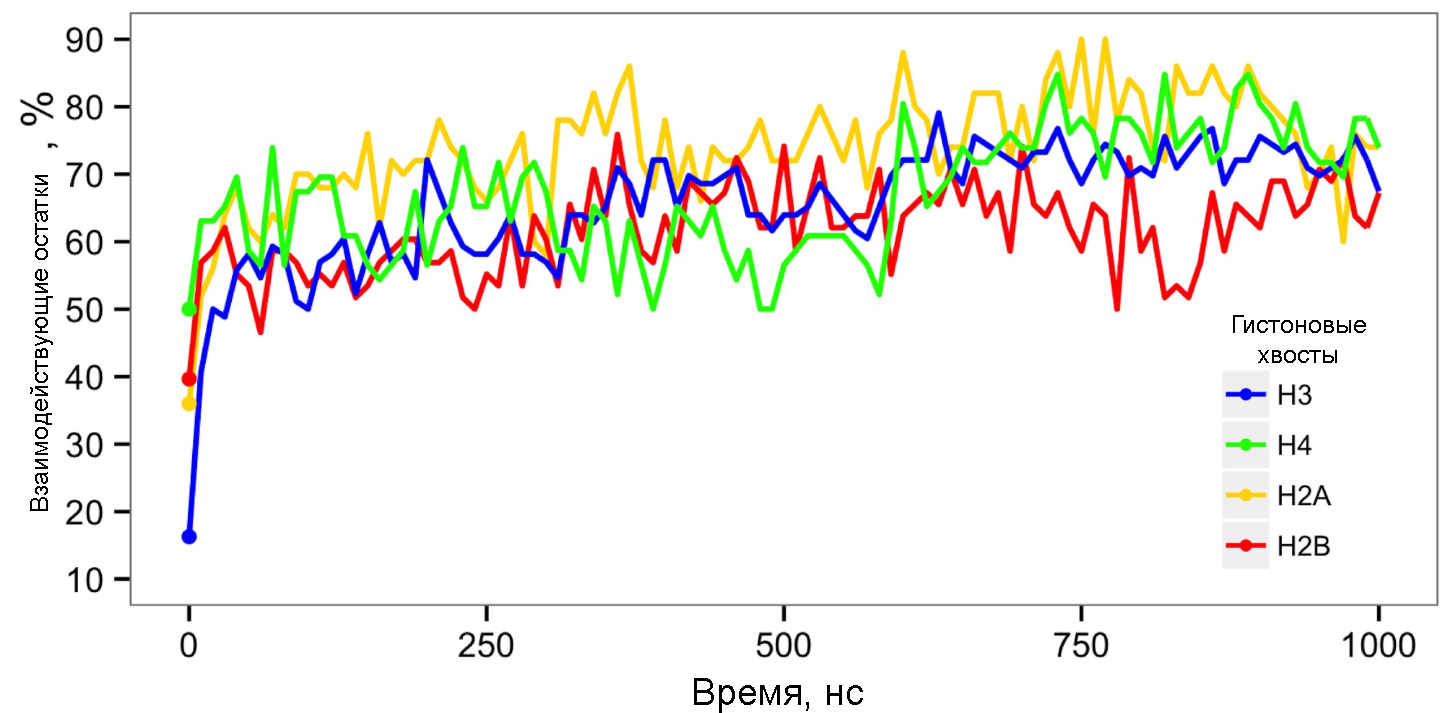
\includegraphics[width=\textwidth]{images/p2/jmb/part2_2_f4.pdf}
    \caption[Конденсация гистоновых хвостов на ДНК]{Конденсация гистоновых хвостов на ДНК. Доля остатков гистонового хвоста, которые имеют прямые или опосредованные водой взаимодействия с ДНК, представлена как функция времени моделирования. Начальные значения обозначены точками.}
    \label{fig:p2_2_f4}
\end{figure}

\begin{figure} [H]
    \centering
    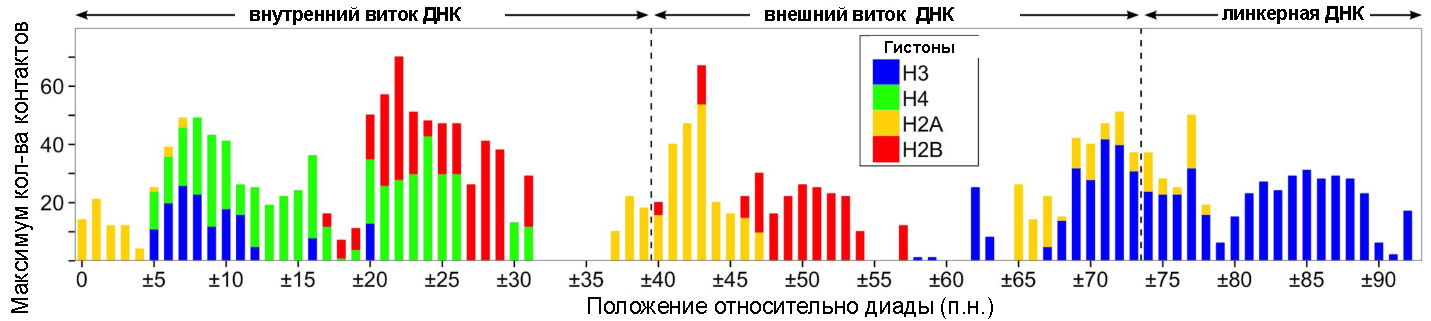
\includegraphics[width=\textwidth]{images/p2/jmb/part2_2_f5.pdf}
    \caption[Доступность ДНК для взаимодействия с гистоновыми хвостами]{Доступность ДНК для взаимодействия с гистоновыми хвостами. Максимальное количество атом-атомных контактов между ДНК и гистоновыми хвостами показано для всех кадров из различных систем моделирования (FN, FNnt и FNbb).}
    \label{fig:p2_2_f5}
\end{figure}



\subsubsection{Хвосты гистонов ``застревают’’ в малых бороздках ДНК и влияют на доступность эпигенетически модифицированных сайтов}
    Конденсация гистоновых хвостов на ДНК в ходе моделирования явно изменила конформационную динамику хвостов и самой ДНК, фактически она напоминала двумерную диффузию на поверхности ДНК с малыми бороздками ДНК, служащими кинетическими ловушками. Несмотря на обширное моделирование, за 1 мкс мы заметили, что хвосты двух копий одного и того же гистона часто исследовали не перекрывающиеся подмножества конформационного пространства. Мы предполагаем, что переключение между различными конформационными подпространствами для таких хвостов происходило во временном масштабе более длительном, чем время нашего моделирования (Рис. \ref{fig:p2_2_f6}). Такое поведение согласуется с экспериментальными данными по химическому  сшиванию и ЯМР гистоновых хвостов \cite{lee_n-terminal_1997,zhou_histone_2012}. Интересно, что в нашем микросекундном моделировании скорость конформационной динамики гистоновых хвостов зависела от их конформации и способа связывания с ДНК. Например, амплитуда колебаний хвоста H3 на одной стороне нуклеосомы, который адсорбируется на линкерной ДНК, была намного выше (из-за гибкости линкерной ДНК) по сравнению с другим хвостом H3, который был компактно свернут на около входа ДНК в нуклеосому. Динамические характеристики гистоновых хвостов в мононуклеосомах и массивах нуклеосом недавно были исследованы с помощью ряда методов, включая твердотельный ЯМР и ЯМР в растворе, дейтеро-водородный обмен \cite{kato_characterization_2009,zhou_histone_2012,gao_histone_2013}. Данные исследования содержат достаточно противоречивые выводы. Принимая во внимание наши результаты, мы предполагаем, что динамика гистоновых хвостов даже в компактных массивах нуклеосом может быть организована неоднородным образом, при этом одни хвосты стабильно свернуты, в то время как другие активно исследуют конформационное пространство.

    Подробный анализ взаимодействий между отдельными боковыми цепями аминокислот и основаниями ДНК указывает на то, что определенные боковые цепи хвостов гистонов могут быть глубоко вставлены в малые бороздки ДНК, взаимодействуя с основаниями ДНК и выступая в качестве якорей, стабилизирующих взаимодействия и ограничивающие конформационную динамику. Наибольшее количество контактов с основаниями ДНК образовано аргининами и лизинами, расположенными внутри гистоновых хвостов. А именно, в основной (FN) модели, следующие остатки показали высокую склонность к взаимодействию с основаниями малой бороздки ДНК: R8 и R26 гистона H3; K16 и R17 гистона H4; R11, K13 и K126 гистона H2A, R29 и R30 гистона H2B. Интересно, что для хвостов H3 и H4 ни одно из этих взаимодействий с основаниями ДНК не наблюдалось в исходной рентгеновской структуре. В то время, как среди контактов белок-ДНК внутри гистонового кора преобладали взаимодействия с фосфатами (в модели FN 82\% - фосфаты, 16\% - сахара, 2\% - основания), в области гистоновых хвостов 17\% контактов - это взаимодействия с основаниями, что значительно больше, чем  количество контактов между основаниями ДНК и гистонами в кристаллической структуре (8\%).

    Следует отметить, что многие упомянутые выше сайты потенциально могут подвергаться посттрансляционным модификациям, включая метилирование аргининов и метилирование и ацетилирование лизинов. Например, два из наиболее важных эпигенетически модифицированных остатков на гистоне H3 (H3K9 и H3K27) расположены рядом с остатками аргинина (H3R8 и H3R26), которые показали высокую тенденцию к встраиванию в малые бороздки ДНК. Следовательно, такие мотивы аргинин-лизин внутри гистоновых хвостов могут влиять на доступность определенных лизинов для эффекторных белков и их способность посттрансляционно модифицироваться.
    
    Если мы проанализируем те сайты, которые устанавливают прямые контакты с нуклеотидами в малой бороздке ДНК в наших моделях, наиболее выраженным является H4K16, который находится в позиции ДНК SHL -1,5. Это хорошо известный сайт ацетилирования, который регулирует компактизацию хроматина и связывание ремоделера ACF \cite{shogren-knaak_histone_2006}. Исследование мононуклеосом методом ЯМР подтвердило гибкость остатков 1-15 хвоста гистона H4, тогда как остатки 16-22 плотно взаимодействуют с нуклеосомным кором и не демонстрируют мобильности в соответствующей шкале времени ЯМР. Более того, было экспериментально подтверждено, что ацетилирование, имитирующее мутацию H4K16Q, которая, согласно нашему исследованию, вероятно, ослабит взаимодействие этого остатка с малой бороздкой ДНК из-за потери положительного заряда боковой цепи, вызывает структурное разупорядочение в этой области \cite{zhou_histone_2012}. В соответствии с нашими наблюдениями, экспериментальное исследование показало, что H4H18 и H4K16 могут быть связаны с позициями ДНК SHL $\pm$1.5 \cite{weng_probing_2014}. Наши наблюдения о связывании малой бороздки с H4K16 также согласуются с более ранними выводами Erler et al. в REMD-моделировании нуклеосом \cite{erler_role_2014}. Совсем недавно Collepardo-Guevara et al. в многомасштабном моделировании показали, что ацетилирование лизина увеличивает содержание вторичных структур в гистоновом хвосте и снижает доступность хвоста для решающих межнуклеосомных взаимодействий, компактизующих хроматиновые волокна \cite{collepardo-guevara_chromatin_2015}, что согласуется с более ранним моделированием конформационного ансамбля фрагментов гистоновых хвостов без ДНК в растворе \cite{potoyan_energy_2011,potoyan_regulation_2012}. Эти результаты также согласуются с более ранней работой по моделированию взаимодействий ДНК с пептидами из H4-хвоста \cite{korolev_h4_2007,korolev_molecular_2014}, в которой авторы предположили, что заряженные группы аргининов и лизинов играют главную роль в притяжении ДНК-ДНК через хвост гистона, образуя мосты между фосфатными группами и взаимодействую с электроотрицательными участками в малой бороздке.

    Наш сравнительный анализ взаимодействий гистонов с ДНК в различных областях нуклеосомы предполагает, что большинство взаимодействий в области глобулярных частей гистонов обеспечивается преимущественно остатками аргинина, в то время как взаимодействия между хвостами гистонов и ДНК почти в равной степени обеспечиваются остатками аргинина и лизина (Рис. \ref{fig:p2_2_f7}). Это не относится к исходной конформации, происходящей из кристаллической структуры NCP, где взаимодействия белок-ДНК через остатки лизина в значительной степени недостаточно представлены. Хотя следует отметить, что в кристаллической структуре NCP дополнительные контакты гистон-ДНК могут формироваться с соседними нуклеосомами в кристаллической решетке, которые мы не включаем в наш анализ. Такая тенденция согласуется со склонностью аргининов находится в малых бороздках ДНК, как это наблюдалось в кристаллических структурах многих комплексов белок-ДНК \cite{rohs_role_2009}. Как видно из рисунка \ref{fig:p2_2_f7}, глицин также преобладает в H3, H2A и особенно в N-концевых хвостах H4, и его карбонильная группа основной цепи может образовывать неспецифические контакты с фосфатами основной цепи ДНК. Важно отметить, что, хотя прямые контакты белков с основаниями ДНК (прямое считывание) обычно считаются почти отсутствующими в нуклеосомах и не влияют на позиционирование нуклеосом, это может быть слишком упрощенной картиной. Например, было показано, что гистоновые хвосты могут вносить вклад в зависимое от последовательности позиционирование нуклеосом \cite{yang_core_2007}. Однако этот эффект не воспроизводился на последовательностях с высоким сродством. Обширные контакты гистоновых хвостов с основаниями ДНК, наблюдаемые в нашем исследовании, могут помочь понять и интерпретировать эти экспериментальные результаты.

\subsubsection{Выпячивание ДНК возле точек входа/выхода модулируется конформациями гистонового хвоста}
    Теперь обратим внимание на анализ связи между конформацией гистоновых хвостов и геометрией нуклеосомной ДНК. В ходе моделирования проявились некоторые изменения в конформации ДНК (Рис. \ref{fig:p2_2_f3}aб). Самая большая замеченная перестройка -- выпячивание ДНК рядом с ее точкой входа в нуклеосому в районе SHL $\pm$6,5. Данную перестройку можно было наблюдать только во временных масштабах более 100 нс, и она была обусловлена различными конформациями гистоновых хвостов (Рисунок \ref{fig:p2_2_f6}). Взаимодействия в этой области ДНК (концевые 10 п.н. коровой ДНК) в основном представлены взаимодействиями с гистоновыми хвостами, а не с глобулярными доменами, что позволяет предположить, что гистоновые хвосты могут оказывать сильное влияние на конформацию ДНК, приводя к потенциальной стабилизации или дестабилизации всей нуклеосомы. Действительно, в моделировании FN-модели терминальная коровая область ДНК вокруг SHL +6,5 образовывала намного больше контактов с гистоновыми хвостами, чем ее симметричный аналог в SHL -6,5 (184 контакта против 64), что вызывало ее стабилизацию и предотвращало выпячивание ДНК. Эта стабилизация, по-видимому, была вызвана обширными взаимодействиями с N-концевым хвостом H3, который формирует компактную вторичную структуру около места входа / выхода ДНК, а также вставкой H2A K126 в малую бороздку ДНК (Рис. \ref{fig:p2_2_f6}). Таким образом С-концевой хвост H2A также может участвовать в стабилизации ДНК. Фактически, недавно было экспериментально обнаружено, что частичная делеция С-концевой области H2A приводит к разворачиванию последних 10 п.н. коровой ДНК \cite{shukla_docking_2011}. В соответствии с этим фактом, колебания концевых частей коровой ДНК были менее ограниченными в нашем моделировании для системы NCPm, которая имела усеченные гистоновые хвосты (Рис. \ref{fig:p2_2_f3}aб).


\begin{figure} [H]
    \centering
    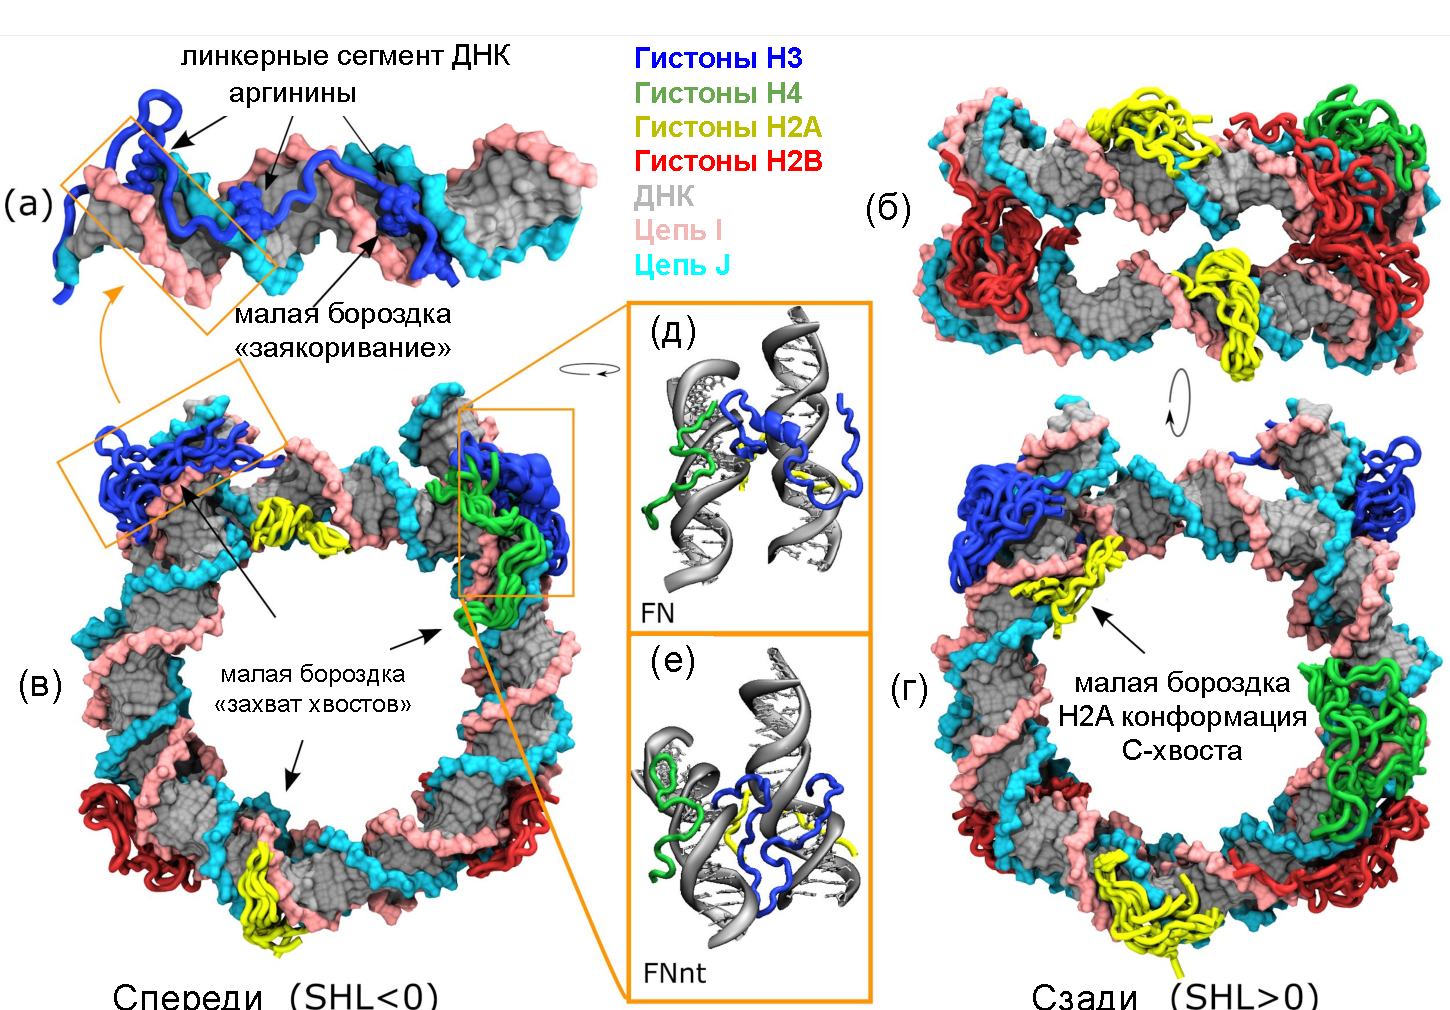
\includegraphics[width=\textwidth]{images/p2/jmb/part2_2_f6.pdf}
    \caption[Типичные паттерны взаимодействия гистоновых хвостов с ДНК]{Типичные паттерны взаимодействия гистоновых хвостов с ДНК, наблюдаемые при МД моделировании. (а) Типичная конформация N-концевого хвоста H3, взаимодействующего с линкерной ДНК. (б) - снизу, (в) - спереди и (г) - виды нуклеосомы с множественными наложенными конформациями гистонового хвоста, наблюдаемыми в течение 1 мкс МД моделирования (изображены каждые 100 нс с отброшенными первыми кадрами 250 нс). (д) формирование $\alpha$-спирали, образованной остатками 21-28 одного из хвостов H3 (цепь A), (е) альтернативное стабильное положение хвоста H3, ``состыкованное'' между супервитками ДНК.}
    \label{fig:p2_2_f6}
\end{figure}

\begin{figure} [H]
    \centering
    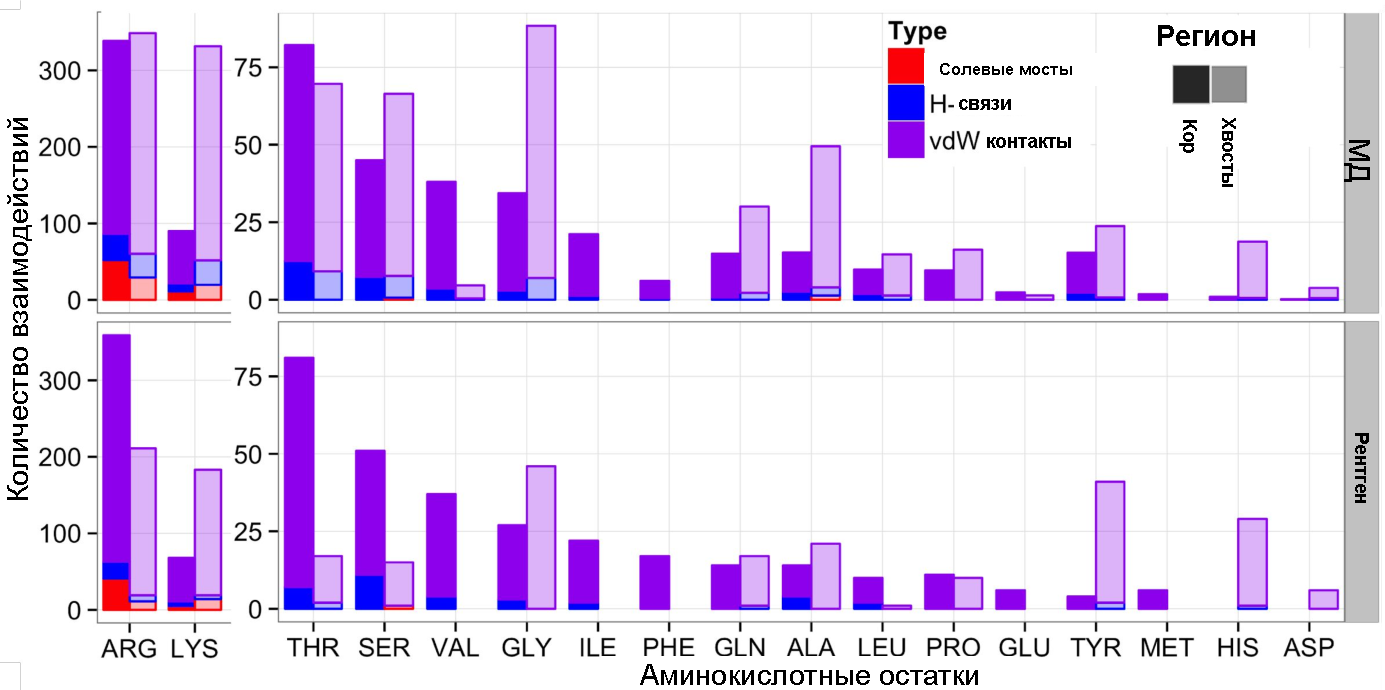
\includegraphics[width=\textwidth]{images/p2/jmb/part2_2_f7.pdf}
    \caption[Взаимодействия белок-ДНК в нуклеосоме]{Количественная оценка взаимодействий белок-ДНК по типу, участку гистона и участвующим аминокислотам.}
    \label{fig:p2_2_f7}
\end{figure}

\begin{figure} [H]
    \centering
    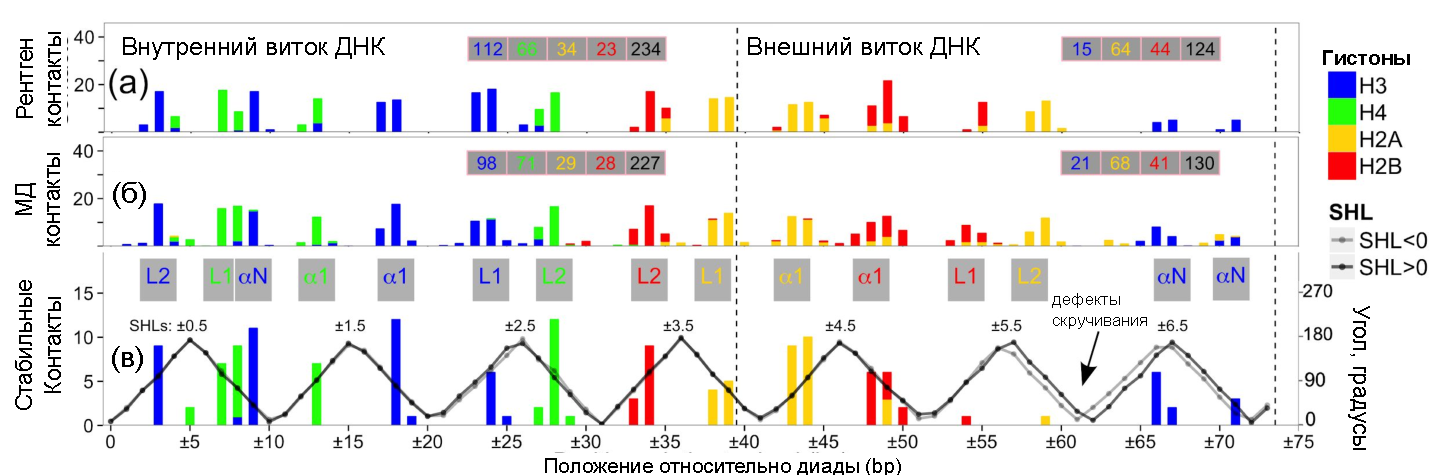
\includegraphics[width=\textwidth]{images/p2/jmb/part2_2_f8.pdf}
    \caption[Взаимодействия белок-ДНК в области нуклеосомного кора]{Взаимодействия белок-ДНК в области нуклеосомного кора. (а) Профиль контактов для рентгеновской структуры, усредненный по двум половинам нуклеосомы. (б) Среднее количество контактов по всем кадрам и по симметричным половинам нуклеосомы. Общее количество контактов для соответствующих участков ДНК и гистонов показано в розовых рамках для графиков (а) и (б). (в) Количество стабильных контактов белок-ДНК. В каждой позиции ДНК указывается количество уникальных стабильных контактов атом-атом, наблюдаемых на любой половине нуклеосомы (т.е. связанные с симметрией стабильные контакты, наблюдаемые в двух половинах нуклеосомы, подсчитывались только один раз, асимметричные контакты вносились индивидуально). Структурные элементы сайтов связывания ДНК аннотированы в верхней части этого графика разными цветами, соответствующими разным типам гистонов. Черные и серые кривые показывают периодичность вращения ДНК в структуре нуклеосом, усредненной по траектории.}
    \label{fig:p2_2_f8}
\end{figure}





\subsubsection{Сайты связывания ДНК в гистоновом коре демонстрируют возможность перестройки, сопровождающейся образованием дефектов кручения ДНК}
    В наших предыдущих разделах мы говорили о взаимодействиях между гистоновыми хвостами и ДНК; в этом разделе мы обсудим взаимодействия гистонов с ДНК, вовлекающие глобулярные домены гистонов, и их связь с перестройками геометрии ДНК. Из анализа кристаллической структуры NCP известно, что ДНК имеет семь пар симметричных сайтов связывания, где малая бороздка ДНК обращена к октамеру гистонов. В каждом сайте связывания ключевой аргинин вставлен в малую бороздку в большинстве случаев, за исключением канонических аргининов R49 из обеих копий H3, которые расположены слишком далеко, чтобы их можно было вставить в малую бороздку в районе SHL $\pm$6.5. В то же время это место имеет небольшое количество контактов с гистоновым ядром (Рис. \ref{fig:p2_2_f8}а,б). Наш анализ динамики взаимодействий гистон-ДНК показал, что этот канонический H3R49 действительно может быть вставлен в соответствующую малую бороздку из-за выпячивания ДНК в районе SHL $\pm$6.5, описанной ранее. Этому выпячиванию, по-видимому, способствовало образование дополнительных и перестройка существующих контактов между $\alpha$N-спиралью H3 и ДНК. Чтобы понять последствия этих изменений для общей геометрии ДНК, мы построили график эффективного вращения пар оснований ДНК относительно положения суперспиральной оси (Рис. \ref{fig:p2_2_f8}в). Мы наблюдали сдвиг в общем скручивании ДНК на одну пару оснований вокруг SHL -6/-6,5, а в случае модели NCPm такие сдвиги наблюдались в области от SHL -5,5 до конца коровой ДНК. Подобные сдвиги в геометрии скручивания ДНК ранее были названы ``твист-дефектами'' \cite{edayathumangalam_nucleosomes_2005}. Некоторые экспериментальные исследования показали, что нуклеосома существует в растворе как смесь различных состояний твист-дефектов, и только некоторые из них могут быть увидены в кристаллических структурах путем изменения основной последовательности ДНК, ее длины или добавления интеркалирующих агентов \cite{edayathumangalam_nucleosomes_2005}. В нашем исследовании мы впервые смогли наблюдать образование таких дефектов \textit{in silico} и описать атомистические детали, лежащие в основе связи между геометрией ДНК и взаимодействиями гистон-ДНК.
    
    Чтобы выяснить закономерности взаимодействий в различных сайтах связывания гистонов с ДНК, мы вычислили количество так называемых стабильных контактов (см. Методы). Как видно на рисунках \ref{fig:p2_2_f8}a-в, количество контактов между гистоновым кором и внутренним супервитком ДНК было почти вдвое больше, чем количество контактов с внешним витком ДНК. Это согласуется с более легким разворачиванием внешнего витка ДНК в экспериментах с единичными молекулами \cite{hall_high_2009,brower-toland_mechanical_2002}. Более того, рисунок \ref{fig:p2_2_f8} показывает четкую иерархию между различными каноническими сайтами связывания. Сайты связывания вокруг SHL $\pm$0,5 и SHL $\pm$4,5 имеют наибольшее количество динамически стабильных контактов в соответствии с картированием с высоким разрешением взаимодействий белок-ДНК в нуклеосомах, полученным путем механического растягивания ДНК. Последние эксперименты показали, что наиболее сильные взаимодействия гистон-ДНК происходят вокруг диады и в районе расположения $\pm$40 пар оснований от диады \cite{hall_high_2009}.
    
    Первый сайт связывания гистонов с ДНК вокруг SHL $\pm$0,5 образован петлями L1/L2 димера H3-H4, с дополнительным взаимодействием, исходящим от N-конца $\alpha$N-спирали H3, что делает этот сайт очень особенным с точки зрения его уникальной специфической организации. Различия между паттернами связывания гистонов с ДНК наблюдались на картах нуклеосом по всему геному, и недавно с помощью геномного анализа позиционирования нуклеосом был обнаружен необычный сигнал относительно содержания A|T/G|C в нуклеосомной ДНК в девяти парах оснований от центра нуклеосомы \cite{brogaard_map_2012}. Предполагалось, что это может быть связано с внедрением H3R40 глубоко в малую бороздку ДНК, либо с образованием специфичных для последовательности контактов с основаниями \cite{davey_does_2013}. Однако мы не наблюдали таких контактов в микросекундном масштабе времени, и H3R40 взаимодействовал с фосфатами ДНК, а не с основаниями.
    
    Второй высокостабильный сайт связывания вокруг SHL $\pm$4.5 образован двумя $\alpha$1-спиралями димера H2A-H2B, тогда как сайты связывания ДНК с наименьшим числом стабильных взаимодействий локализованы на SHL $\pm$6.5, SHL $\pm$5.5 и SHL $\pm$1.5. Карта контактов гистонов с ДНК согласуется с профилем флуктуаций ДНК (Рис. \ref{fig:p2_2_f9}), а флуктуации ДНК показывают видимое увеличение при SHL $\pm$1,5. Это согласуется с повышенной конформационной гибкостью ДНК в этих сайтах при связывании малых молекул или белков показанной в недавних экспериментах. Эти эксперименты показали, что SHL $\pm$1,5 является местом связывания ионов тяжелых металлов и интеркалирующих противоопухолевых агентов \cite{tan_nucleosome_2011}. Отсутствие стабильных взаимодействий вокруг SHL $\pm$5.5/$\pm$6.5 также соответствует увеличению флуктуаций ДНК. Колебания на самом конце коровой ДНК несколько меньше, что объясняется их стабилизацией через N- и С-концевые хвосты H3 (см. Предыдущие разделы). Малая стабильность и высокая гибкость сайтов связывания SHL $\pm$5.5 и SHL $\pm$6.5 может указывать на то, что эти сайты вносят лишь небольшие энергетические барьеры при разворачивании ДНК из нуклеосомы. Биологически значимый процесс, который основан на таком постепенном разрыве контактов ДНК-гистонов, включает транскрипцию РНК-полимеразами, которая может происходить без вытеснения нуклеосом \cite{studitsky_mechanism_1997}. Нуклеосомный барьер для транскрипции, исследованный с помощью паттернов транскрипционного паузирования, показал, что первый барьер встречается полимеразой, когда передний край полимеразы входит в область примерно в 40 п.н. от диады \cite{jin_synergistic_2010}. Данный факт согласуется с представлением о том, что первые два сайта связывания почти не представляют барьера для транскрипции.


\begin{figure} [H]
    \centering
    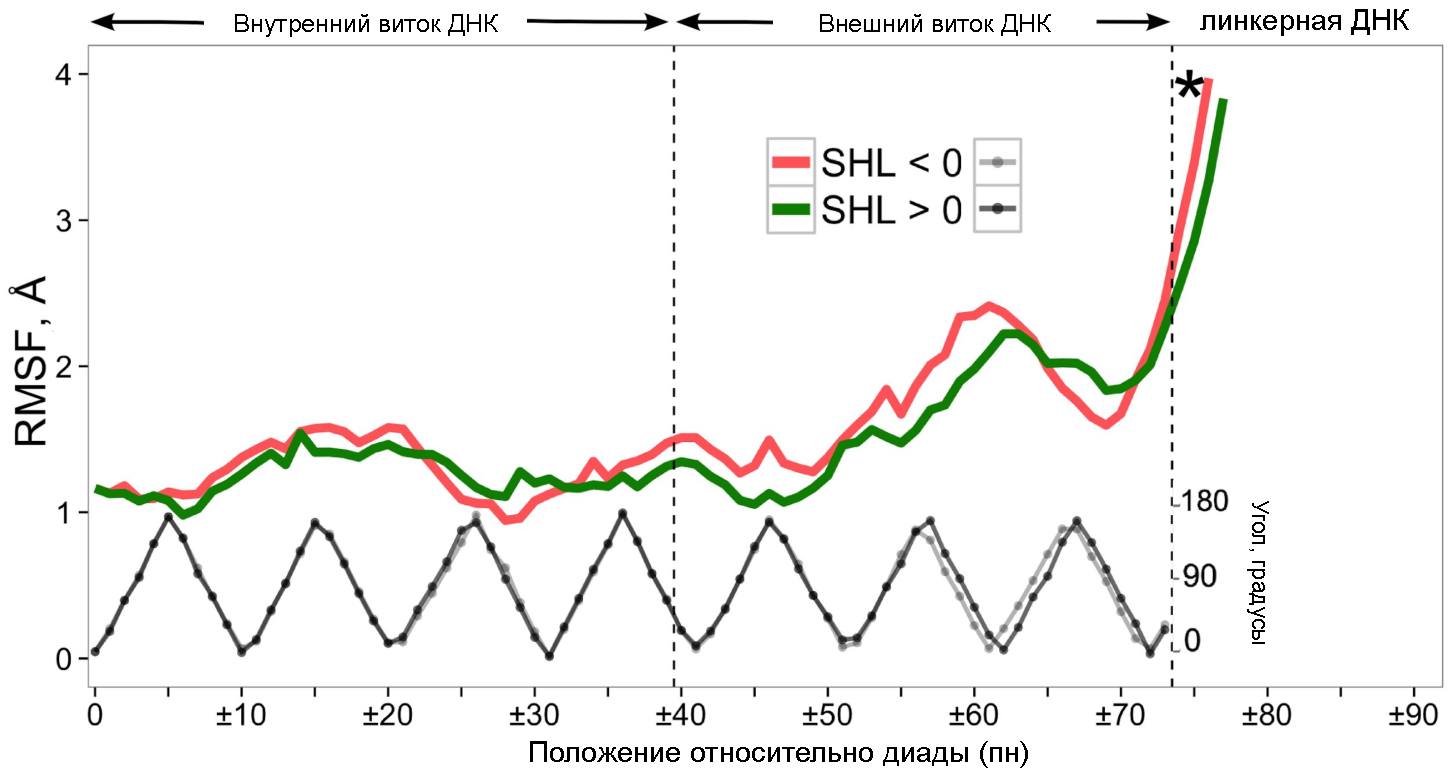
\includegraphics[width=\textwidth]{images/p2/jmb/part2_2_f9.pdf}
    \caption[Флуктуации ДНК в нуклеосоме]{Флуктуации ДНК в нуклеосоме. RMSF центров пар оснований для двух симметричных половин нуклеосом (красная и зеленая кривые); черные и серые кривые показывают периодичность вращения суперспирали ДНК. Точки данных, превышающие RMSF 4\AA, не показаны. Звездочкой обозначена та же цепь, что и на рисунке \ref{fig:p2_2_f3}.}
    \label{fig:p2_2_f9}
\end{figure}

\subsection{Обсуждение}
    В данном разделе мы представили молекулярно-динамическое исследование полной модели нуклеосомы с полноразмерными гистоновыми хвостами и линкерными участками ДНК. Мы использовали полноатомное моделирование в явном растворителе и распространили этот подход на микросекундную шкалу времени. Микросекундная шкала времени и многочисленные сравнительные симуляции позволили нам получить представление о функционально значимых перестройках в конформациях нуклеосом, включая связь между конформациями гистоновых хвостов и ДНК.

    Механистические наблюдения, полученные в нашем исследовании, предполагают, что конформационные перестройки внутри коровой ДНК зависят от паттернов взаимодействий ДНК с гистонами. В частности, мы наблюдали, что N-концевой хвост H3 и C-концевой хвост H2A устанавливают много контактов с коровой ДНК и могут стабилизировать геометрию ее концевой области, подавляя образование локализованных дефектов кручения внутри ДНК. С другой стороны, конформация хвостов, которые выступают из нуклеосомы, способствуют образованию состояний с дефектами кручения, которые могут быть важными промежуточными звеньями в скольжении и ремоделировании нуклеосом \cite{mueller-planitz_nucleosome_2013}. Мы предлагаем наличие механизма, с помощью которого наблюдаемое чрезмерное скручивание ДНК в терминальной области ДНК может представлять собой начальное состояние дефекта кручения ДНК, которое может быть стабилизировано последующими перестройками взаимодействий ДНК в центральной области гистонов. Последующее скольжение нуклеосом может происходить за счет распространения этого дефекта дальше по кору нуклеосомы. Интересно отметить, что несколько исследований по химическому сшиванию мононуклеосом \textit{in vitro} ранее показали, что гистоновые хвосты занимают различные предпочтительные конформации в NCP, нуклеосомах с линкерами и нуклеосомами с гистоном H1 \cite{lee_linker_1998,angelov_preferential_2001}. Данный факт позволяет предположить, что гистоновые хвосты очень чувствительны к наличию/отсутствию линкерной ДНК, гистона H1 и изменений в нуклеосомном окружении.
    
    В соответствии с результатами экспериментов по химическому сшиванию  ДНК с гистонами \cite{angelov_preferential_2001,stefanovsky_laser-induced_1989} мы обнаружили, что гистоновые хвосты легко адсорбируются на линкерную (в основном хвосты H3) и коровую ДНК (в основном хвосты H4, H2B и H2A), и большинство контактов гистонов с ДНК представлено контактами с гистоновыми хвостами. О возможности взаимодействия N-концевых хвостов H3 с линкерной ДНК сообщалось ранее \cite{rhee_subnucleosomal_2014,angelov_preferential_2001}. Фактически, эффективность химического сшивания в NCP оказалась в 3–4 раза ниже для H2A, H2B и H4 и в 10–12 раз ниже для H3 по сравнению с полными нуклеосомами с линкерной ДНК \cite{stefanovsky_laser-induced_1989}. Более того, наше детальное изучение поведения гистоновых хвостов показало, что их динамика в микросекундном масштабе характеризуется ограниченной диффузией на поверхности ДНК и кинетическим захватом хвостовых областей в малых бороздках ДНК. Наблюдаемое стабильное прикрепление гистоновых хвостов к коровой и линкерной ДНК предполагает глубокие последствия для взаимодействий нуклеосом с другими белками хроматина. В самом деле, когда эти белки связываются с гистоновыми хвостами или ДНК, сначала они должны проконкурировать со взаимодействиями ДНК-гистоновый хвост и вытеснить соответствующего партнера. Например, Pilotto et al. недавно экспериментально продемонстрировали элегантную практическую иллюстрацию этой концепции на примере комплекса LSD1-CoREST, который действует как деметилаза H3K4 \cite{pilotto_interplay_2015}. Было высказано предположение, что этот комплекс связывается с нуклеосомой через свою субъединицу CoREST, которая вытесняет хвост H3 с ДНК. Это смещение критически необходимо для того, чтобы сделать метилированный H3K4 доступным для взаимодействий с его субъединицей LSD1. Можно предположить, что такие механизмы могут быть использованы для организации перекрестного взаимодействия между множественными сайтами связывания на гистоновых хвостах, включая сайты ПТМ и их соответствующих партнеров по связыванию \cite{ruthenburg_multivalent_2007,nishi_crosstalk_2015}.
    
    Атомистические детали связывания гистонового хвоста с ДНК, выявленные в ходе нашего исследования, дополнительно показали, что этому процессу способствует вставка закрепляющих боковых цепей аргинина и лизина в малые бороздки ДНК. Это, в свою очередь, повлияло на те остатки, которые служат эпигенетически модифицированными сайтами в хвостах гистонов, или на остатки, расположенные рядом с ними (например, H3K9, H3K27, H4K16 и H3R8, H3R26 и т.д.). Присутствие множества сайтов связывания на одном хвосте гистонов и окклюзия боковой цепи малыми бороздками может вызывать кооперативные эффекты. А именно, связывание одного партнера с его сайтом связывания на ДНК или сайтом гистонового хвоста может вызвать смещение гистонового хвоста от ДНК и, таким образом, облегчать связывание другого партнера. Подобные эффекты могут быть вызваны посттрансляционными модификациями, такими как метилирование аргинина и особенно ацетилирование лизина, которые не способствуют встраиванию этих остатков в малую бороздку и, таким образом, могут способствовать конформационной гибкости и доступности связывания гистоновых хвостов. Наблюдаемые эффекты помогают наметить дальнейший план экспериментальных исследований, которые должны прояснить сложное динамическое взаимодействие между посттрансляционными модификациями гистонов и доступностью гистоновых хвостов для связывания эффекторных белков.

\subsection{Материалы и методы}
\subsubsection{Построение начальной модели}
    В качестве отправной точки мы использовали рентгеновскую кристаллическую структуру высокого разрешения (1,9\AA) коровой частицы нуклеосомы, образованную рекомбинантными вариантами канонических коровых гистонов \textit{X. laevis}и модифицированной $\alpha$-сателлитной ДНК человека (PDB ID 1KX5 \cite{davey_solvent_2002}). Для создания полной нуклеосомной модели с линкерными сегментами ДНК с помощью программы NAB был сконструирован прямой дуплекс B-ДНК $(AGTC)_5$ длиной 20 п.н. \cite{macke_thomas_modeling_1997}. Используемая линкерная последовательность ДНК сбалансирована по количеству гибких и жестких динуклеотидов \cite{olson_dna_1998}. Она была прикреплена к основной ДНК на обоих концах NCP. Один из хвостов гистона H3 был слегка повернут, чтобы избежать стерических столкновений с линкерной ДНК (угол $\Psi$ Lys36 был установлен на -35 градусов) (Рис. \ref{fig:p2_2_f1}a). Минималистичная модель NCP (NCPm) была получена из той же кристаллической структуры путем усечения гистоновых хвостов в сайтах, указанных на рисунке \ref{fig:p2_2_f2} треугольниками. Все модели были явно сольватированы в прямоугольной ячейке с минимальным расстоянием между растворенным веществом и границами ячейки в 20\AA, за исключением системы FNbb (таблица 1), для которой использовался порог в 100\AA. В системы добавляли ионы натрия для нейтрализации, а затем добавляли дополнительные ионы натрия и хлора в концентрации 150 мМ по отношению к объему воды, за исключением системы FN1M, где использовалась концентрация 1 М. Точная соответствующая объемная концентрация ионов была оценена непосредственно из данных моделирования. Кристаллографические молекулы воды остались в системе, а все кристаллографические ионы были удалены. Состояния протонирования аминокислот определяли на основании значений pK их растворов при нейтральном pH, остатки гистидина считали нейтральными и протонировали на $\epsilon$-азотах. Модель FNnt была идентична модели FN, но имела нейтрально заряженные белковые концы для изучения устойчивости МД-моделирования к небольшим возмущениям. Структуры исходных моделей представлены на рис. \ref{fig:p2_2_f1}а. На выбор NaCl в качестве соли для нашего моделирования повлияло его обычное использование в экспериментах с нуклеосомами \textit{in vitro}, а также в протоколах сборки нуклеосом \cite{dyer_reconstitution_2004}.

\subsubsection{Протоколы моделирования и выбор силового поля}
    Силовое поле CHARMM36 использовалось для ДНК и белка \cite{best_optimization_2012,hart_optimization_2012}, параметры TIP3P для молекул воды и скорректированные параметры  Луо и Ру для ионов \cite{luo_simulation_2010}. Выбор силового поля всегда является деликатным вопросом из-за известных и неизвестных приближений, используемых в силовом поле, а также постоянными усилиями по улучшению силового поля, предпринимаемых разработчиками. В случае нуклеосом проблема осложняется необходимостью сочетать точные модели белков и ДНК, а также обеспечивать реалистичное моделирование взаимодействий с растворителем. Ниже мы кратко обсудим несколько недавних современных исследований о поведении различных силовых полей при моделировании нуклеосом.
    
    Точность силового поля белка, по-видимому, особенно важна для моделирования поведения изначально неупорядоченных гистоновых хвостов. Систематические исследования биомолекулярных силовых полей \cite{lindorff-larsen_systematic_2012} показали, что определенные силовые поля (например, CHARMM27, AMBER ff03) сверхстабилизируют спиральную конформацию пептидов, и поэтому эта проблема была решена в пересмотре силового поля для белков CHARMM36 \cite{best_optimization_2012}. Кроме того, несколько недавних исследований поставили под сомнение применимость силовых полей белков для специфического моделирования гистоновых хвостов \cite{erler_role_2014,collepardo-guevara_chromatin_2015,potoyan_energy_2011}. Например, Erler et al. показали, что разные версии силовых полей AMBER могут приводить к разному динамическому поведению гистоновых хвостов \cite{erler_role_2014}. Collepardo-Guevara et al. сравнили результаты моделирования с использованием современных силовых полей, включая CHARMM36, с данными ЯМР по динамике гистонового хвоста и пришли к выводу, что все силовые поля дают почти идентичные результаты \cite{collepardo-guevara_chromatin_2015}.

    Силовое поле ДНК необходимо для правильного воспроизведения конформационных переходов ДНК при моделировании нуклеосом. Параметризация силовых полей нуклеиновых кислот оказывается более сложной задачей, чем аналогичная задача для белков. В настоящее время известно, что силовые поля как CHARMM, так и AMBER воспроизводят стабильную динамику ДНК в микросекундном масштабе времени и за его пределами \cite{galindo-murillo_convergence_2015}. Однако точное воспроизведение экспериментальных результатов по зависимой  деформируемости ДНК от последовательности с использованием доступных силовых полей все еще остается нерешенной проблемой \cite{perez_frontiers_2012}.
    
    Наши модельные системы были подготовлены с помощью программы VMD \cite{humphrey_vmd_1996}, а моделирование МД было выполнено с помощью пакета NAMD 2.9 \cite{phillips_scalable_2005}. Для моделирования при постоянной температуре использовался подход динамики Ланжевена с шагом интегрирования 2 фс, параметром демпфирования 0,5 $пс^{-1}$ и T = 310K. Поддержание давления в 1 атм было реализовано методом Ланжевена. Моделирование проводилось с жесткими ковалентными связями, и ван-дер-ваальсовы взаимодействия постепенно выключались на расстоянии от 10 до 12\AA. В электростатических расчетах использовался метод PME с шагом сетки 1\AA, кубической интерполяцией, отсечкой в реальном пространстве 12\AA и параметром толерантности $10^{-6}$. Использовались периодические граничные условия. Для устранения диффузии нуклеосом к атомам C-$\alpha$ гистоновых фолдов H3 (номера остатков 64-78, 86-114, 121-131) применялись небольшие позиционные ограничения в 0,003 ккал/моль/$A^2$. Чтобы избежать расплетания пар оснований на концах ДНК в моделировании NCPm, использовали ограничивающий потенциал в виде искусственной стенки, чтобы сохранить расстояние между центрами масс оснований в концевых парах оснований в пределах 120\% от начального.

    Все системы были подвергнуты минимизации энергии и первоначальному уравновешиванию. Затем проводилось моделирование до времени моделирования 1 $\mu$с. Кадры траектории сохранялись каждые 100 пс. Мы запускали расчеты параллельно на высокопроизводительных компьютерных кластерах/суперкомпьютерах, используя эффективное распараллеливание, доступное в NAMD. Скорость моделирования варьировалась в зависимости от моделируемой системы, количества процессоров и архитектуры машины. Для справки: система модели FN моделировалась параллельно на 384 ядрах ЦП в течение 120 дней со скоростью $\sim$8 нс/день.
%21 страница

\subsubsection{Анализ траекторий}
    Анализ и визуализация траектории выполнялись с использованием набора библиотек и скриптов собственной разработки, написанных на TCL, Python и R, которые использовали возможности VMD \cite{humphrey_vmd_1996} и 3DNA \cite{lu_3dna_2008} для общего и специфического анализа структуры ДНК. Для структурного анализа нуклеосом отдельные кадры траектории были наложены на исходную кристаллическую структуру, путем минимизации значения среднеквадратичного отклонения (RMSD) между положениями атомов C-$\alpha$ спиралей гистоновых фолдов. Анализ конформации ДНК проводили по отношению к нуклеосомной суперспиральной системе отсчета, определяемой ее диадной осью и суперспиральной осью. Периодичность вращения ДНК в нуклеосоме определяли путем расчета угла между вектором пары оснований (соединяющим атомы N1 и N9 соседних оснований в паре оснований) и суперспиральной осью нуклеосомы. Максимумы и минимумы значений периодичности вращения соответствовали целочисленным и полуцелым значениям SHL.
    
    Подробный анализ взаимодействий гистонов с ДНК проводился для каждого кадра траектории (первые кадры 250 нс не учитывались как начальный период конформационного уравновешивания) путем анализа положений соответствующих атомов. Контакты (SC) между двумя атомами гистона и ДНК определялись как контакты между тяжелыми атомами на расстоянии менее 3,9\AA. Контакты были дополнительно классифицированы следующим образом: солевые мостики (SB) включают два заряженных неводородных атома на расстоянии менее 3,9\AA; водородные связи (HB) были определены как связи между донорными (D) и акцепторными (A) атомами с водородом между ними (DH-A), где расстояние между D и A было меньше 3,5\AA, а DH-A угол составлял больше 150 градусов; контакты Ван-дер-Ваальса (vdW) были определены как контакты между атомами, которые не были связаны водородными связями и не образовывали солевой мостик; и опосредованные водой взаимодействия (WM) определялись как взаимодействия между неводородными атомами ДНК или гистонами, которые образуют водородную связь с одной и той же молекулой воды. Мы также ввели понятие стабильных контактов между ДНК и белком, чтобы описать контакты, которые сохранялись во время моделирования. А именно, они были определены как отдельные пары атомных контактов между ДНК и молекулами белка, которые присутствовали более чем в 80\% кадров траектории после начального периода конформационного уравновешивания.

\subsubsection{Соглашения об описании структуры нуклеосом}
    Позиции пар оснований ДНК были пронумерованы относительно центральной пары оснований (называемой диадой), ее положение принималось равным нулю. Вращательная ориентация двойной спирали ДНК полуколичественно описывается параметром сверхспирального расположения (SHL) (Рис. \ref{fig:p2_2_f1}a), который мы расширяем, чтобы включить не только коровую ДНК (SHL от 0 до $\pm$7), но и линкерную ДНК (SHL до $\pm$9). Исходные 147 пар оснований ДНК NCP называются ``коровой ДНК'', а области, где коровая ДНК соединяется с линкерной ДНК, называются сайтами входа/выхода ДНК. Мы различаем две части в каждом гистоне: область хвоста (как указано на рисунке \ref{fig:p2_2_f2}) и остальную часть, называемую глобулярной частью гистона. Ключевыми элементами глобулярных областей являются спирали гистоновых фолдов $\alpha$1, $\alpha$2 и $\alpha$3 \cite{baxevanis_variety_1995} и петли L1, L2, как показано на рисунке \ref{fig:p2_2_f2}.


\subsubsection{Благодарности}
Исследования данного раздела были поддержаны программами внутренних исследований Национальной медицинской библиотеки и Национального института рака, Национальных институтов здоровья; и Российским научным фондом [грант № 14-24-00031] (разработка алгоритмов визуализации нуклеосом). Автор был поддержан программой сотрудничества между США и Россией в области биомедицинских наук. В этом исследовании использовались высокопроизводительные вычислительные возможности кластера Biowulf Linux в Национальном институте здравоохранения, Бетесда, Мэриленд \url{http://biowulf.nih.gov}. Данное исследование было частично поддержано Суперкомпьютерным центром МГУ им. М.В. Ломоносова и вычислительными ресурсами суперкомпьютера Hexagon Cray XE6m-200, в университете Бергена и норвежском метацентре высокопроизводительных вычислений (NOTUR).










\section{Моделирование коровых частиц нуклеосом на масштабах свыше 10 микросекунд}
\textit{Данный раздел описывает работы, выполненные в 2017-2020 годах, являющиеся продолжением работ предыдущего раздела. Работы основаны на использовании более современных компьютерных архитектур с использованием графических процессоров и учитывают серьезный объем новых экспериментальных данных, опубликованных в 2017-2020 годах. Интерактивные материалы раздела доступны по ссылке} \url{http://intbio.github.io/nucl_MD_15mus/}.

% новая статья
\subsection{Введение}
Многие химические и физические сигналы регулируют обработку генетической информации в живых клетках.
У эукариот эта регуляция в основном происходит на уровне нуклеосом - последовательных отрезков ДНК, обернутых вокруг октамеров гистоновых белков \cite{kornberg_chromatin_1974,olins_spheroid_1974}. Четыре типа гистонов (H3, H4, H2A, H2B) образуют два типа димеров (H3-H4, H2A-H2B). Четыре димера образуют октамер с двойной осью симметрии (диадной осью) \cite{burlingame_crystallographic_1985}. Как известно из кристаллографических исследований, примерно 147 пар оснований ДНК резко изгибаются вокруг октамера в $\sim$1,7 витка левой суперспирали, формируя коровую частицу нуклеосомы (NCP) \cite{luger_crystal_1997} (Рис. \ref{fig:p2_3:f1}а).

При формировании нуклеосом жесткая макромолекула ДНК с персистентной длиной около 50 нм должна резко изгибаться до радиуса кривизны всего в 5 нм. Это возможно благодаря электростатическому взаимодействию отрицательно заряженной ДНК с положительно заряженными гистонами, дополненному индивидуализированным паттерном взаимодействия белок-ДНК на атомном уровне в 14 сайтах связывания ДНК (по 7 с каждой стороны NCP). Эти сайты связывания расположены в положениях, где малая бороздка ДНК обращена к поверхности октамера и обычно присутствует боковую цепь остатка аргинина, которая выступает в пространство малой бороздки. Общая энергия взаимодействий гистонов с ДНК в нуклеосомах оценивается как не менее 23 ккал/моль \cite{onufriev_nucleosome:_2019}.
Стабильность нуклеосом может варьироваться на 2-4 ккал/моль в зависимости от гибкости последовательности ДНК \cite{thastrom_sequence_1999}, которая, как было показано, зависит от содержания GC, наличия гибких динуклеотидных ступеней YR, участков поли (dA:dT), эпигенетических модификации оснований ДНК, таких как 5-метилцитозин и т. д. \cite{ngo_asymmetric_2015,chua_mechanics_2012,zhurkin_sequence-dependent_1985,segal_genomic_2006}. Еще одним важным фактором являются вариации последовательности гистонов. Несмотря на то, что гистоновые белки одни из самых консервативных белков в эволюционном смысле, они подвержены множеству функционально значимых вариаций, включая посттрансляционные модификации (ПТМ) \cite{zhao_comprehensive_2015} и изменение последовательности за счет включения вариантов, изоформ и мутаций гистонов \cite{draizen_histonedb_2016,singh_replication-dependent_2018,nacev_expanding_2019}.

Представление о нуклеосомах как о средстве простой компактизации ДНК теперь устарело.
% Благодаря своей роли в обеспечении доступа к ДНК, нуклеосомы играют ключевую роль в эпигенетической регуляции экспрессии генов.
Различные режимы АТФ-зависимой и АТФ-независимой динамики нуклеосом, модулируемые гистоновым составом и последовательностью ДНК, обеспечивают богатый динамический ландшафт для регуляции генома \cite{armeev_linking_2019}. Например, скольжение нуклеосом с помощью АТФ-зависимых ремоделеров хроматина \cite{paul_regulation_2018} или их реконфигурация с помощью РНК-полимераз \cite{kujirai_transcription_2020,gaykalova_structural_2015} в значительной степени вовлечены в транскрипцию и ее регуляцию. Пассивная динамика нуклеосом также участвует во многих процессах. Новаторские эксперименты Джона Видома показали, что временное отворачивание ДНК от октамера гистонов может быть использовано факторами транскрипции для доступа к их сайтам связывания \cite{li_rapid_2005}. Недавние исследования методами FRET \cite{gansen_high_2018,sabantsev_direct_2019}, ЯМР \cite{sinha_distortion_2017, kitevski-leblanc_investigating_2018}, крио-ЭМ \cite{li_mechanism_2019,bilokapic_structural_2018} и масс-спектрометрии\cite{hada_histone_2019,sanulli_hp1_2019,sinha_distortion_2017} свидетельствуют о том, что существуют более тонкие режимы конформационной динамики нуклеосом, которые воспринимаются и используются белками хроматина. Например, кручение ДНК внутри NCP обеспечивает путь для АТФ-зависимого ремоделирования нуклеосом \cite{bowman_remodeling_2019,li_mechanism_2019}. Внутренняя динамика (пластичность) гистонового ядра также участвует в этом процессе (хотя на этот счет и ведутся дискуссии) \cite{sinha_distortion_2017,yan_structures_2019,armache_cryo-em_2019}. Сообщалось, что подавление этой динамики путем введения сайт-специфичных дисульфидных сшивок в отдельные димеры H3-H4 ингибирует передвижение нуклеосом ремоделером SNF2h, увеличивает вытеснение октамера комплексом RSC \cite{sinha_distortion_2017}, блокирует термически индуцированную диффузию нуклеосом вдоль ДНК \cite{bilokapic_structural_2018} и даже нарушает компактизацию хроматина белком HP1 \cite{sanulli_hp1_2019}. Эти результаты свидетельствуют о том, что октамер гистонов может принимать конформации, альтернативные тем, которые наблюдаются в рентгеновских структурах. Действительно, используя передовые методы крио-ЭМ, Bilokapic et al. недавно наблюдали некоторые альтернативные конформации нуклеосом с развернутой ДНК, наклоненными гистоновыми $\alpha$-спиралями и общей сжатой формой NCP \cite{bilokapic_structural_2018,bilokapic_histone_2018}. Еще большие внутренние флуктуации в структуре октамера гистонов предполагают эксперименты по химической сшивке лизинов \cite{hada_histone_2019} и эксперименты FRET с высоким разрешением\cite{gansen_high_2018}.


Эти и другие исследования подчеркнули существование нового уровня динамической сложности нуклеосом, связанного с атомистическими деталями структуры. Однако структурная интерпретация этих результатов все еще остается не вполне ясной. \textit{In silico} подходы, такие как моделирование методом молекулярной динамики (МД), являются мощными инструментами, которые могут дополнять экспериментальные методы и помочь механистически интерпретировать экспериментальные результаты с высоким уровнем детализации. До сих пор моделирование с помощью МД применялось для изучения распределения ионов вокруг нуклеосом и их гидратации \cite{materese_counterion_2009}, деталей разворачивания ДНК, скольжения и разборки нуклеосом \cite{ettig_dissecting_2011, rychkov_partially_2017, zhang_exploring_2016, winogradoff_molecular_2019,brandani_dna_2018,lequieu_silico_2017}, динамики гистоновых хвостов\cite{erler_role_2014, shaytan_coupling_2016,chakraborty_molecular_2018,morrison_conformation_2018}, эффектов посттрансляционных модификаций гистонов \cite{fenley_modulation_2018,li_investigating_2018,rajagopalan_structural_2017} и их вариантов \cite{bowerman_unique_2019}, эффектов влияния последовательности ДНК \cite{sun_tmb_2019} на динамику нуклеосом, взаимодействия между олигонуклеосомами \cite{collepardo-guevara_chromatin_2015} и гистоном H1 \cite{ozturk_chromatosome_2020,perisic_sensitive_2019} и т. д. Из-за вычислительной сложности такого рода расчетов часто прибегают к упрощениям (например, удаляют гистоновые хвосты, используют неявные модели растворителя или крупно-зернистое представление молекулярной системы), либо ограничивают временные рамки моделирования. В настоящее время наиболее известные МД исследования нуклеосом в полноатомном приближении были ограничены несколькими микросекундами времени моделирования \cite{winogradoff_molecular_2019,chakraborty_molecular_2018} даже с применением специализированных суперкомпьютеров, таких как ANTON. Однако предполагается, что важные функциональные переходы в структуре нуклеосом происходят в масштабе времени от микросекунды до миллисекунды \cite{gansen_high_2018}. Новые режимы функциональной динамики в этих временных масштабах все еще ждут подробных структурных исследований с помощью МД-моделирования.

В работе данного раздела, мотивированные различными новыми экспериментальными доказательствами ранее неизвестных способов конформационной динамики и пластичности нуклеосом, мы систематически исследовали равновесную динамику нуклеосом с помощью полноатомного МД-моделирования на масштабе времени 10 микросекунд и более.
Насколько нам известно, это первый случай, когда такие длинные динамические траектории анализируются для максимально реалистичных атомистических моделей NCP с полноразмерными гистоновыми хвостами при физиологической температуре и ионной силе. С помощью специально разработанных алгоритмов анализа траекторий (проекция координат в системе отсчета нуклеосом, расчет относительного скручивания ДНК, анализ стабильных контактов и т. д.) мы выявили новые режимы динамики и пластичности нуклеосом. Мы наблюдаем реконфигурацию и разворачивание концов ДНК в нуклеосомах, опосредованных гистоновыми хвостами H3 и H2A, образование дефектов кручения в ДНК и сдвиг ориентационного положения для части коровой ДНК, структурную пластичность ядра гистона в соответствии с недавними экспериментальными наблюдениями. В данном разделе также обсуждается значение наших результатов для понимания ремоделирования нуклеосом и организации структуры хроматина более высокого порядка.


\subsection{Материалы и методы}
\subsubsection{Молекулярно-динамические расчеты}
Моделирование проводилось с использованием пакета GROMACS 2018.1 с поддержкой графических ускорителей \cite{abraham_gromacs:_2015} с силовым полем Amber ff14SB \cite{maier_ff14sb_2015}, дополненным поправками parmbsc1 \cite{ivani_parmbsc1_2016} для ДНК и поправками ионных параметров CUFIX \cite{yoo_new_2018}. Начальные координаты были получены из соответствующих структурных файлов в базе данных PDB (см. таблицу \ref{tbl:p2_3:systems}). Для моделирования системы NCP$_{147}$ конформация хвостов гистонов для одной половины NCP (цепи E, F, G, H) была скорректирована, чтобы соответствовать конформации симметричных цепей на другой половине NCP (цепи A, B, C, D). Для моделирования с усеченными гистоновыми хвостами хвосты усекались согласно позициям, изображенным на рисунке \ref{fig:p2_3:f1}д. Сайты усечения были выбраны таким образом, чтобы удалить гибкие части хвостов гистонов, при этом оставляя некоторые части близкие к глобулярному ядру, которые устанавливают стабильные контакты с ДНК или гистонами (например, N-хвосты H3 и H2B, выступающие между супервитками ДНК или H2A C-хвост, взаимодействующий с димером H3-H4). Для моделирования с фиксированными гистоновыми фолдами, C $\alpha$-атомы спиралей $\alpha1$, $\alpha2$ и $\alpha3$ во всех гистонах удерживались в их исходных положениях с использованием гармонического потенциала с силовой постоянной 1000 кДж/моль/нм$^2$. Все системы были помещены в ячейку для моделирования в виде усеченного октаэдра с периодическими граничными условиями, установленными на расстоянии не менее 2 нм от атомов NCP. Следующим шагом в ячейку добавлялись молекулы воды модели TIP3P \cite{jorgensen_comparison_1983} для сольватации NCP, затем были добавлены ионы Na и Cl, чтобы нейтрализовать заряд и довести ионную силу до 150 мМ (Рис. \ref{fig:p2_3:f1}б). Сконструированные системы были минимизированы по энергии и уравновешены в несколько этапов с постепенным снятием ограничений с тяжелых атомов в течение 1 нс. Температуру поддерживали на уровне 300 K с использованием схемы масштабирования скорости \cite{bussi_canonical_2007}, а давление на уровне 1 бар с помощью баростата Парринелло-Рамана \cite{parrinello_polymorphic_1981} Моделирование проводилось параллельно на суперкомпьютере ``Ломоносов-2'' \cite{voevodin_supercomputer_2019} с использованием 8 вычислительных узлов, каждый из которых имеет 14 ядер ЦП и один графический процессор NVidia Tesla K40. Моделирование происходило со средней скоростью 60 нс в день.
% 450000 CPU + 32000 часов GPU на каждые 10 микросекунд моделирования

\subsubsection{Анализ траекторий}
Скрипты для анализа были написаны на Python 3 с интеграцией функций GROMACS (предварительная обработка траектории), MDAnalysis (манипуляции с координатами, трехмерное выравнивание) \cite{michaudagrawal_mdanalysis_2011}, VMD (визуализация) \cite{humphrey_vmd_1996} и 3DNA (определение центров пар оснований ДНК, расчет параметров шага пар оснований и пар оснований) \cite{lu_3dna_2003}.

Для анализа геометрии нуклеосом важной концепцией является нуклеосомальная система координат, состоящая из вектора сверхспиральной оси (OZ, вычисленный из пути ДНК \cite{shaytan_coupling_2016}) и вектора диадной оси псевдосимметрии (OY, определяемый как перпендикуляр, соединяющий OZ с центр центральной пары оснований ДНК). Вместе с вектором OX, определенным как векторное произведение OY и OZ, эти три вектора формируют систему координат нуклеосомы (СКН) (Рис. \ref{fig:p2_3:f1}a). СКН была определена для исходной рентгеновской структуры 1KX5, все другие структуры и конформации были выровнены с ней путем минимизации среднеквадратичного отклонения (RMSD) между C $\alpha$ -атомами $\alpha$-спиралей гистонового фолда ($\alpha1$, $\alpha2$, $\alpha3$). Используя СКН проекции координат атомов на разные плоскости системы координат, можно визуализировать и вычислить параметр относительного кручения ДНК (локальное кручение) \cite{shaytan_hydroxyl-radical_2017}. Последняя характеристика представляет вращение ДНК относительно поверхности октамера гистонов и полезна для отслеживания вращательного позиционирования ДНК и дефектов кручения ДНК.

Для анализа  контактов ДНК-гистоны контакты атом-атом рассчитывали как пары тяжелых атомов (не водородов) с расстоянием менее 4 \AA. Также с помощью MDAnalysis были рассчитаны водородные связи и водные мостики.


\subsection{Результаты и обсуждение}

\subsubsection{Обзор поведения моделируемых систем}

Нами было осуществлено моделирование ряда систем коровых частиц нуклеосом (NCP) на основе различных PDB структур.
Список систем приведен в таблице \ref{tbl:p2_3:systems}. Данные системы включают системы как с полноразмерными гистонами, так и системы с обрезанными хвостами в положениях согласно рисунку \ref{fig:p2_3:f1}д. Особенностью моделей на основе различных PDB структур является различная длина ДНК, которая укладывается на гистоновых октамер: 145, 146 либо 147 пар оснований. Данные структуры обладают концами ДНК, которые находятся в одинаковых положениях, однако в нуклеосомном коре ДНК испытывает растяжение, либо сжатие на 1-2 нуклеотида в положениях SHL $\pm$5 или SHL $\pm$2. Такие области растяжения или сжатия называют дефектами кручения (twist defects). Также нами была промоделирована система с фиксированными C$\alpha$-атомами $\alpha 2$-спиралей гистонов для изучения влияния подвижности гистонов на подвижность ДНК. На рисунках \ref{fig:p2_3:f1}а,б представлены основные обозначения элементов нуклеосомного кора, а также вид системы в ячейке для моделирования с растворителем и ионами.

Общий вид динамики некоторых систем отражен на рисунке \ref{fig:p2_3:f1}в,г. Интерактивные траектории доступны по адресу \url{http://intbio.github.io/nucl_MD_15mus/}. К важным особенностями динамики систем без хвостов на временах порядка 10-15 микросекунд можно отнести: 1) наблюдение откручивания ДНК от гистонового ядра (такого рода эффекты не наблюдаются на временах в несколько микросекунд), 2) релаксацию дефектов кручения ДНК в районе SHL $\pm$5. К важным особенностями динамики систем с гистоновыми хвостами на временах порядка 10-15 микросекунд можно отнести: 1) наблюдение откручивания ДНК от гистонового ядра (в меньших масштабах, чем в системах без гистоновых хвостов), 2) переключение хвостов между различными положениями на ДНК, 3) влияние конформации хвостов на моды откручивания ДНК. Ниже мы подробнее рассмотрим некоторые полученные результаты. 


\begin{figure}[H]
    \centering
    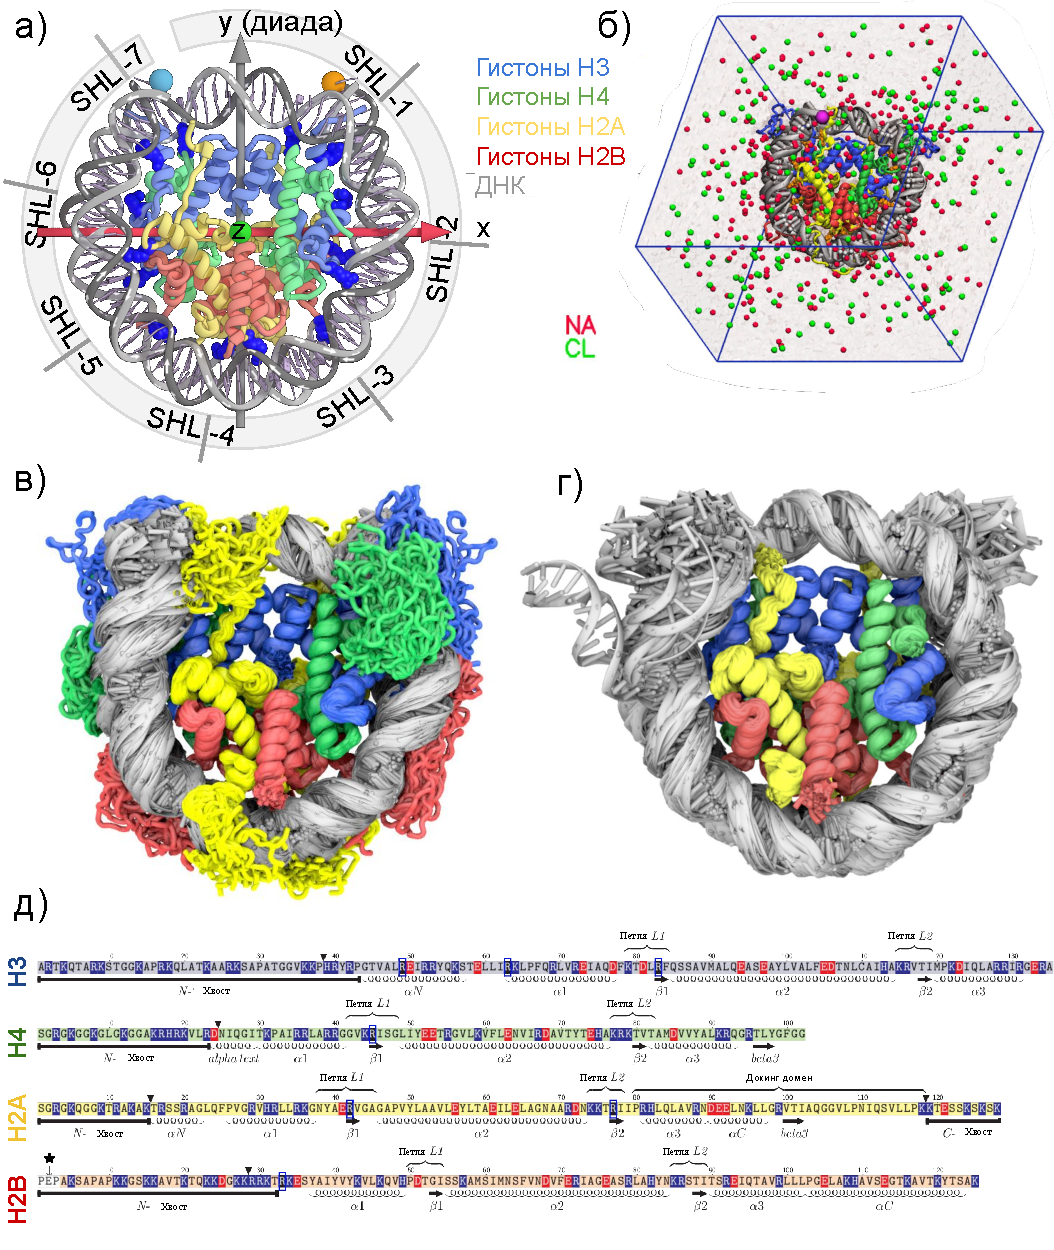
\includegraphics[width=0.95\textwidth]{images/p2/10ms/fig1.pdf}
    \caption[Системы нуклеосом моделируемые на временах более 10 мкс]{Системы нуклеосом моделируемые на временах более 10 мкс. а) Ключевые оси нуклеосомной системы отсчета. б) Вид моделируемой системы в ячейке с растворителем и ионами. c) Наложение кадров системы NCP$_{147} $каждые 100 нс. г) Наложение кадров NCP$^{nt}_{145}$ каждые 100 нс. д) Последовательность коровых гистонов и особенности их вторичной структуры ($ \alpha $ - спирали, $ \beta $ -листы, петли, гибкие хвосты гистонов). $ \blacktriangledown $ отмечает позиции обрезания хвостов в модели с усеченными хвостами; аргинины, боковые цепи которых вставлены малые бороздки ДНК отмечены синими рамками; синим отмечены - положительно заряженные остатки, красным - отрицательно заряженные остатки. $*$ отмечает PEP-конец H2B, который отсутствует в рекомбинантном варианте белка.}
    \label{fig:p2_3:f1}
\end{figure}

\begin{table}[p]
\caption{Список моделируемых систем}
\label{tbl:p2_3:systems}
\begin{threeparttable}
\begin{tabular}{lcp{8cm}c}
\hline
\textbf{Имя}& \textbf{PDB ID}\tnote{a} & \textbf{Описание}&\textbf{Время, мкс}\\ \hline\hline
NCP$_{147}$ & 1KX5 & 147 п.н. псевдосимметричной $\alpha$-сателлитной ДНК, гистоны полной длины в симметричном стартовом состоянии & 13.0  \\ \hline
NCP$^{fixed}_{147}$  & 1KX5 & Такая же как NCP$_{147}$, но C$\alpha$-атомы гистоновых фолдов ограничены в движении &  5.0  \\ \hline
NCP$^{nt}_{147}$ & 1KX5 & Такая же как NCP$_{147}$, но гистоновых хвосты обрезаны\tnote{b} &  10.0  \\ \hline
NCP$^{nt}_{146}$ & 1AOI & 146 п.н. $\alpha$-сателлитная ДНК, обрезанные гистоновые хвосты\tnote{b} & 7.0 \\ \hline
NCP$^{nt}_{145}$ & 3LZ0 & 145 п.н. 601-ой последовательности ДНК, обрезанные гистоновые хвосты\tnote{b} & 13.5  \\ \hline
\end{tabular}
\begin{tablenotes}
     \item[a] Иденификатор структуры, использованной для создания системы, из базы данных PDB.
     \item[b] Сайты обрезки хвостов определены на рис. \ref{fig:p2_3:f1}д.
   \end{tablenotes}
\end{threeparttable}
\end{table}


\subsubsection{Механизмы отворачивания и приворачивания ДНК}

Для анализа отворачивания ДНК от гистонового октамера нами был разработан подход определения количества отвернуты пар нуклеотидов ДНК для каждого кадра траектории. Для каждой пары нуклеотидов вычислялось ее ближайшее расстояние до какой-либо пары нуклеотидов кристаллической структуры. Количество отвернутых пар нуклеотидов с каждого конца определялось как максимальна длина сегмента ДНК от конца ДНК в котором расстояние для всех нуклеотидных пар от любых кристаллических положений было более 7 \AA. На основе данной меры были построены графики зависимости величины отворота ДНК от времени (Рис. \ref{fig:p2_3:f2_new}, Рис. \ref{fig:p2_3:f2}a,б и интерактивные материалы \url{http://intbio.github.io/nucl_MD_15mus/}).

Для систем без гистоновых хвостов ДНК сохраняла исходное привернутое положение в течение начального времени моделирования. Для разных расчетов и сторон нуклеосомы оно колебалось от 0.8 мкс до 4, 6 и более 7 мкс (см. Рис. \ref{fig:p2_3:f2_new}). Для системы с гистоновыми хвостами отворачивание началось на 4-ой микросекунде расчетов. Величина отворота ДНК составляла порядка 12-13 пар нуклеотидов, а в случае систем без хвостов иногда достигала 28 пар нуклеотидов. Рассмотрим в начале механизмы отворота ДНК в системе без хвостов. Анализ стабильных контактов гистонов и нуклеосом показывает, что конец ДНК в нуклеосомном коре формирует плотные контакты и удерживается взаимодействиями с аминокислотными остатками H3 гистона, в особенности H3Y41, H3R42, H3T45, которые находятся в области, которую мы назовем областью ``защелки'' концов ДНК \ref{fig:p2_3:f6}. Плотные взаимодействия в этой области удерживают конец ДНК в NCP. При отвороте ДНК данные взаимодействия нарушаются и ДНК переходит во флуктуирующее состояние, в котором величина отворота быстро меняется в наносекундном диапазоне (см. Рис. \ref{fig:p2_3:f2_new}, состояние \textbf{2}). В некоторых случаях плотные контакты застежки с ДНК восстанавливаются и система переходит в кристаллоподобное состояние (например в системе NCP$_{145}^{nt}$ на третьей наносекунде моделирования). Однако может произойти реконфигурация области защелки в гистоне H3 в состояние, не способное к плотному связыванию ДНК. Это приводит к тому, что флуктуационное состояние становится более долгоживущим и сопровождается также флуктуациями области H3 хвоста (см. Рис. \ref{fig:p2_3:f2_new}, состояние \textbf{2b}). Это флуктуационное состояние может разрешаться в кристаллоподобное состояние ДНК, когда остатки H3 смогут сформировать плотные контакты с флуктуирующим концом ДНК. Более детальный визуальный анализ взаимодействия гистона H3 с концом ДНК показал, что стабильное кристаллоподобное состояние ДНК возникает, когда ряд остатков входят в малую бороздку ДНК. В кристаллической структуре это H3R49, H3Y41, H3H39. Интересно, что в нашем моделировании в ряде систем (NCP$_{145}^{nt}$, NCP$_{145}^{nt}$) кристаллоподобное состояние ДНК также реализовывалось в состоянии, когда вместо H3H39 в малую бороздку заходил H3К40, который в кристалле взаимодействует с малой бороздкой другого супервитка (см. Рис. \ref{fig:p2_3:f2_new}, состояние \textbf{1b}). Дальнейшему откручиванию ДНК препятствовал стабильный сайт связывания с гистонов H2A в районе позиции -59, с которой контактируют остатки H2AK75, H2AT76, H2AR77 из L2 петли. На 14-ой микросекунде в системе NCP$_{145}^{nt}$ наблюдался дальнейший отворот до уровне 26-28 отвернутых пар оснований с диссоциацией контактов данного сайта(см. Рис. \ref{fig:p2_3:f2_new}, состояние \textbf{3}). Данный факт требует дальнейшего исследования. Масштаб флуктуаций ДНК в системе без хвостов представлен на рисунках \ref{fig:p2_3:f1}в,г. Важной особенностью является то, что ДНК откручивается не только в плоскости нуклеосомного диска, но и имеет компонент смещения вдоль суперспиральной оси нуклеосомы. Более подробно взаимоотношение смещения конца ДНК вдоль оси Х и Z представлено на рисунке \ref{fig:p2_3:f1}ж. Существенной корреляции между смещениями не наблюдается, однако очевидно, что при больших параметрах отворота наблюдается в основном состояния с некоторым компонентом смещения вдоль оси суперспирали в направление противоположное от внутреннего супервитка ДНК. Данный факт можно объяснить стерическим и электростатическим отталкиванием витков ДНК.

В отличие от систем без гистоновых хвостов, система с хвостами ведет себя несколько по другому (Рис. \ref{fig:p2_3:f1}б,д,е). Мы также наблюдали откручивание до 12-14 пар оснований с конца ДНК, однако существуют существенные отличия. Во-первых, величина отклонения открученных пар нуклеотидов от их кристаллического пути была меньше из-зи того, что гистоновые хвосты оказывали удерживающее воздействие на конформацию ДНК и ее возможность отклонятся в различных направлениях. Во-вторых, флуктуации ДНК между состояниями с различной степенью откручивания были менее выражены по амплитуде, опять же из-за воздействия гистоновых хвостов, главным образом N-хвоста гистона H3 и С-конца гистона H2A. Наличие гистоновых хвостов приводит к расщеплению динамического состояния отворота-приворота 12 концевых нуклеотидов, наблюдаемого в системе без хвостов, на ряд подсостояний определяемых конформацией гистоновых хвостов. Рисунок \ref{fig:p2_3:f1}и иллюстрирует среднее время приворота ДНК из состояний с заданной величиной отворота. Из рисунка видно, что наличие гистоновых хвостов серьезным образом влияет на увеличение времени приворота ДНК. Для величины отворота в 10 пн время возрастает с 20-40 нс до $\sim$100 нс. Гистоновые хвосты также существенным образом влияют на механизм отворачивания ДНК. Мы наблюдали, что область ``защелки'' H3 гистона также, как и в случае системы без хвостов, теряет контакты с сегментом ДНК вблизи входа-выхода, однако, потери этих контактов способствует внедрение N-конца гистона H3 между супервитками ДНК. Хвост H3 с одной стороны образует дополнительные контакты с ДНК, но с другой стороны способствует замещению стабильных контактов с область H3-``защелки''. Этот же эффект приводит к тому, что в отличие от системы без гистоновых хвостов, хвост H3 может препятствовать быстрому привороту ДНК из отвернутого положения в привернутое.

Более подробно динамика взаимодействия ДНК с H3-``защелкой'' и взаимодействие хвостов гистонов с концами нуклеосомной ДНК представлена на рисунке \ref{fig:p2_3:f3}.

\begin{figure} [H]
    \centering
    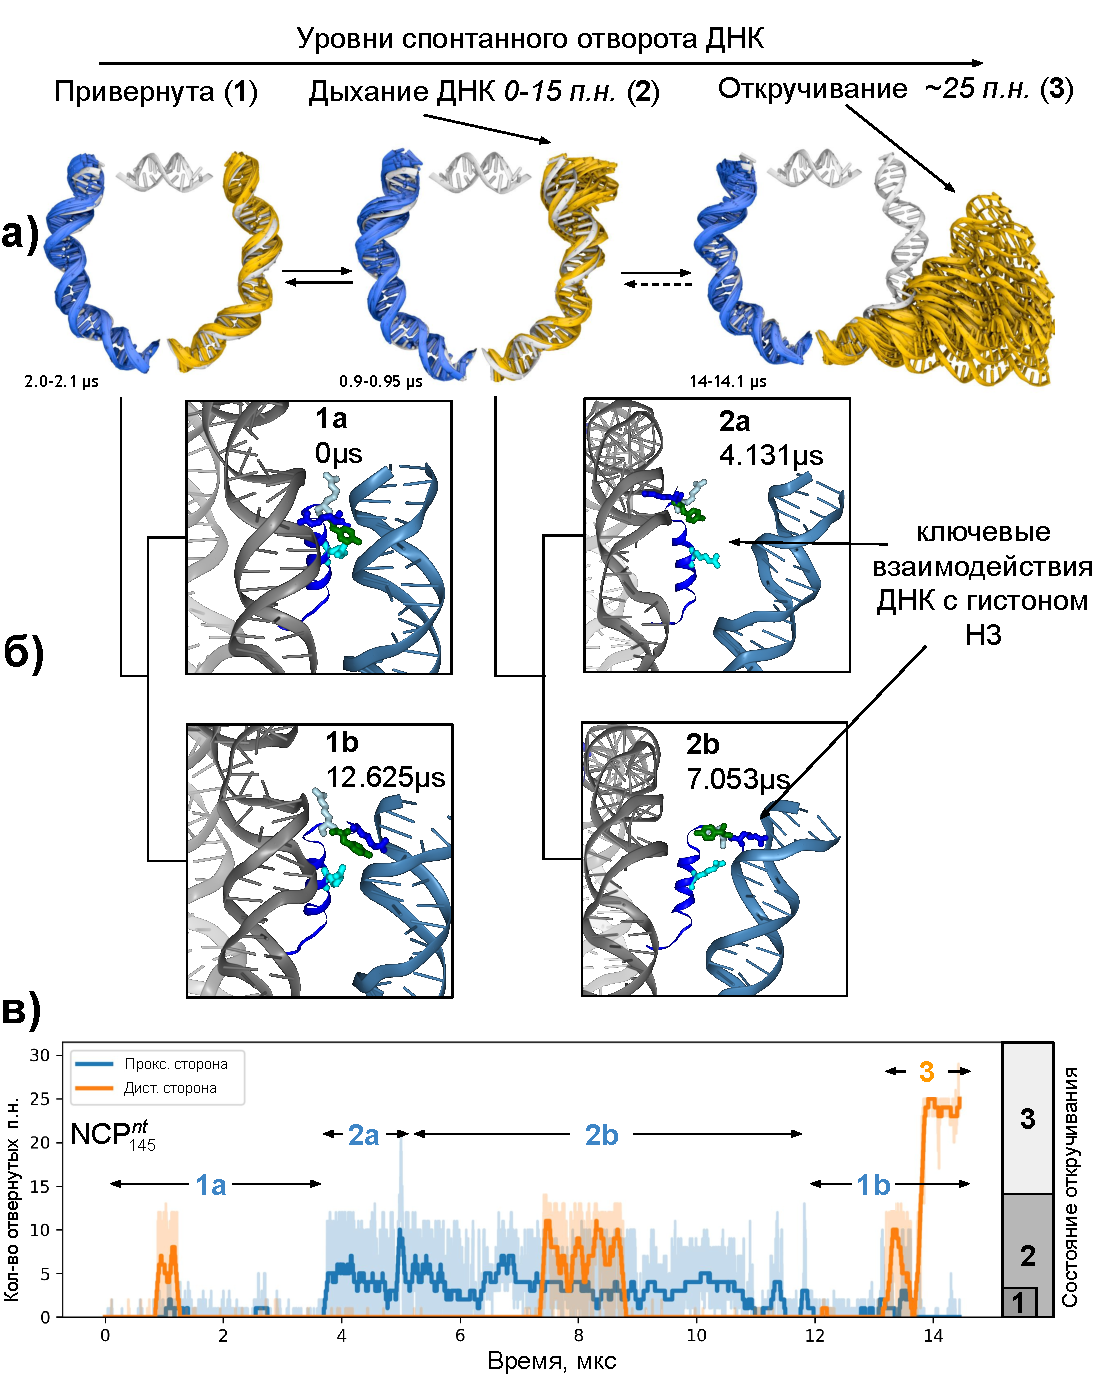
\includegraphics[width=\textwidth]{images/p2/10ms/fig2_new.pdf}
    \caption[Динамика отворота ДНК в нуклеосоме с укороченными гистоновыми хвостами]{Динамика отворота ДНК в нуклеосоме с укороченными гистоновыми хвостами (наблюдаемая в системе NCP$^{nt}_{145}$). Количество пар нуклеотидов отвернутых от октамера гистонов как функция времени моделирования представлена снизу. Критерий отворота ДНК  --  смещение центра пары оснований более, чем на 7 \AA{} от положений оснований в исходной структуре. Наблюдается три состояния \textbf{1-3} (изображены сверху). Для состояний \textbf{1} и \textbf{2} наблюдаются подсостояния, связанные с реориентацией H3 $\alpha$N спирали и области H3-``застежки'' (средний ряд изображений).}
    \label{fig:p2_3:f2_new}
\end{figure}



\begin{figure} [H]
    \centering
    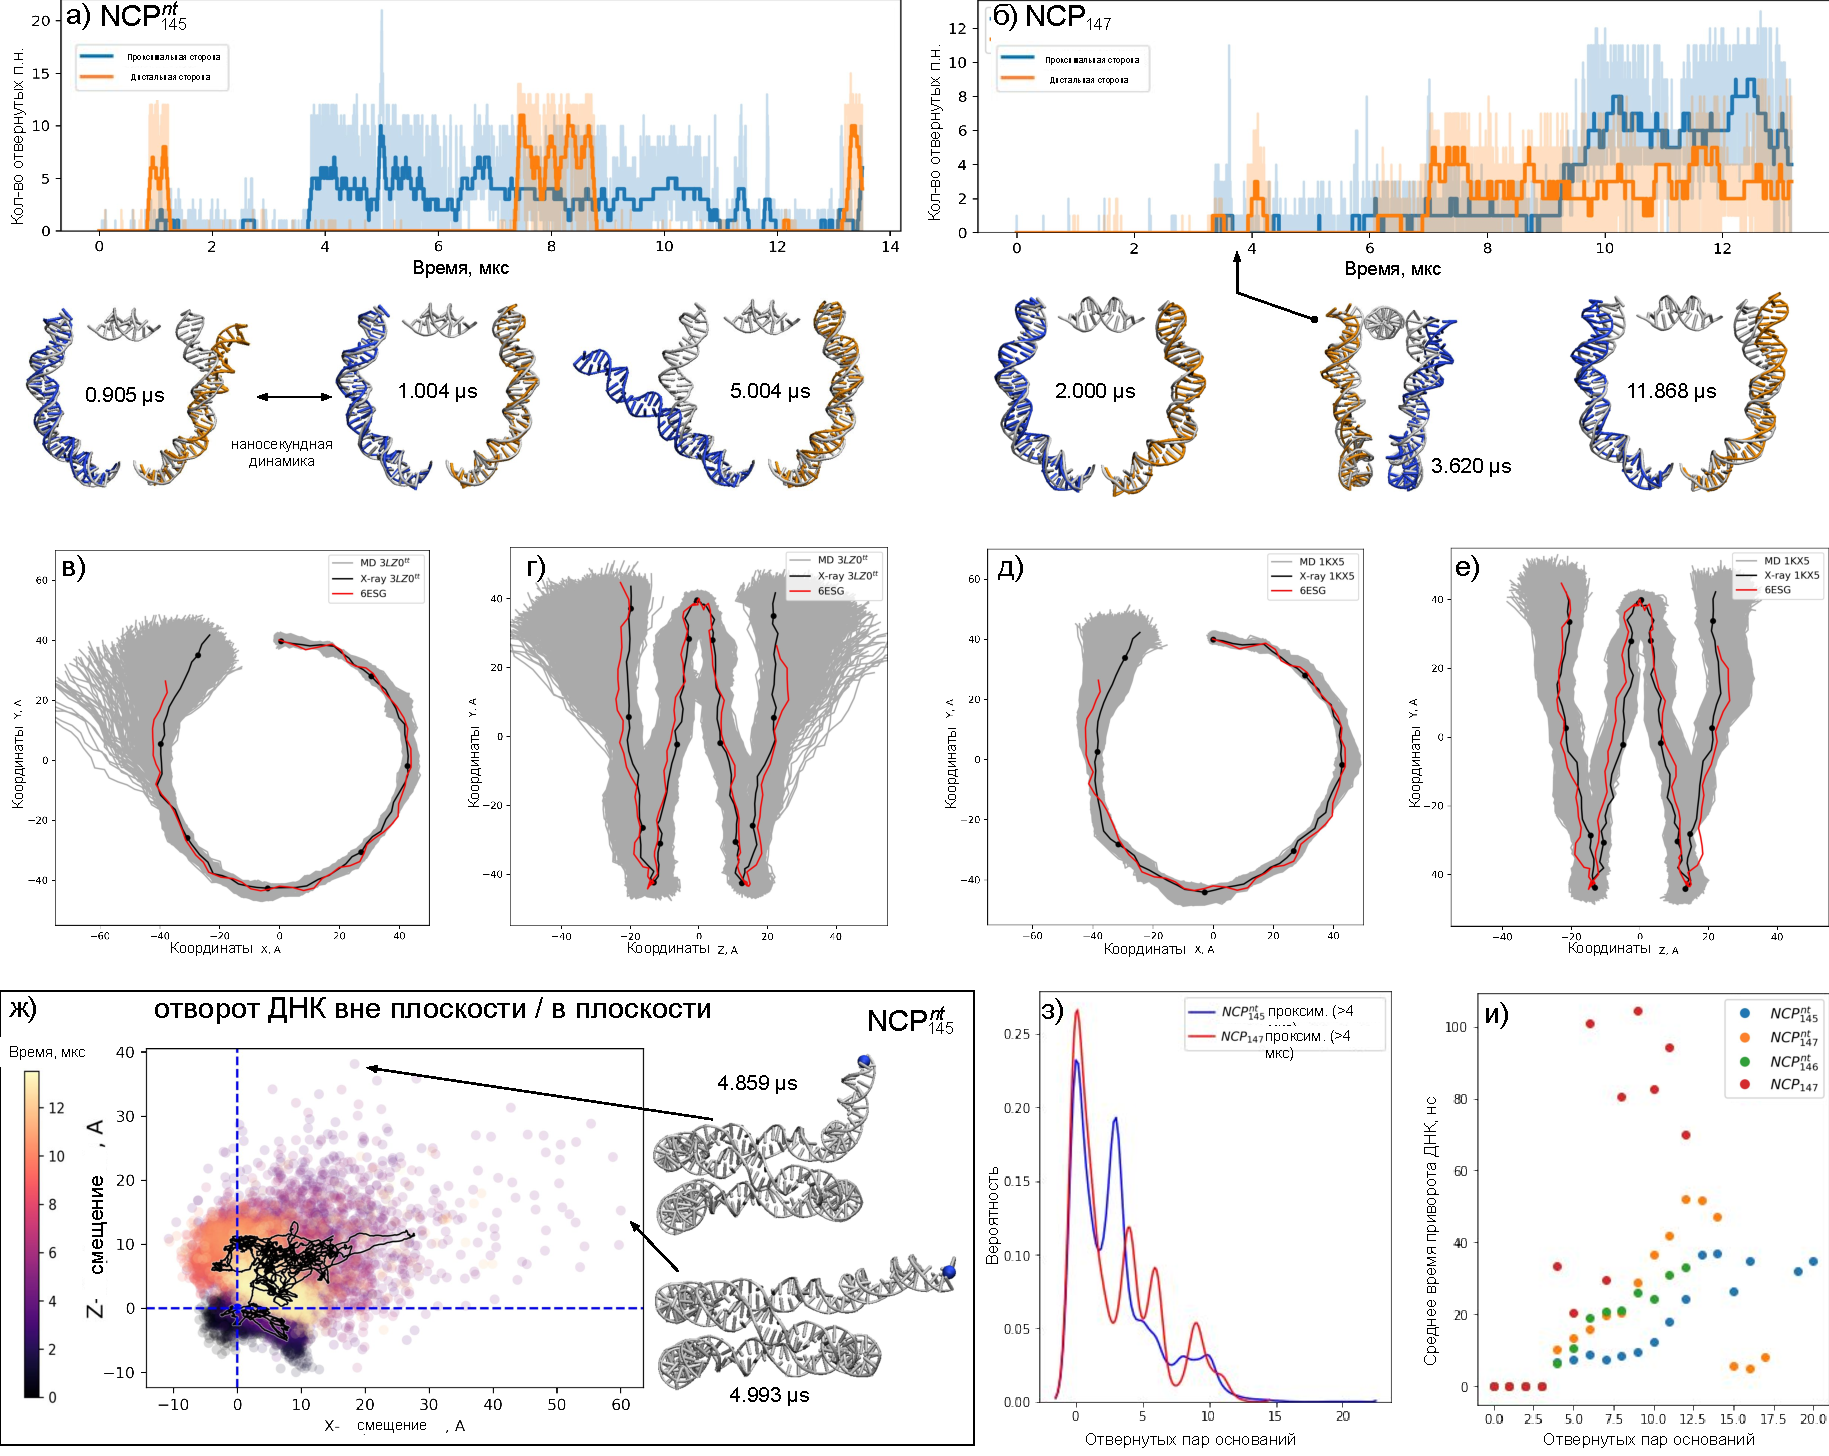
\includegraphics[width=\textwidth]{images/p2/10ms/fig2.pdf}
    \caption[Сравнение характеристик отворота ДНК в нуклеосомах с и без гистоновых хвостов]{Сравнение характеристик отворота ДНК в нуклеосомах с и без гистоновых хвостов. а)-б) отворот ДНК с течением времени для NCP$^{nt}_{145}$ и NCP$_{147}$, определенных как смещение центра пары оснований более, чем на 7 \AA{} от положений оснований в исходной структуре. в-е) Проекции центров пар оснований ДНК на различные плоскости СКН. ж) Смещение проксимального конца ДНК в ходе МД. з) Распределений вероятности отворота ДНК. и) Среднее время приворота ДНК из состояния с определенным отворотом.}
    \label{fig:p2_3:f2}
\end{figure}





\begin{figure}[H]
    \centering
    %DNA ends are coupled to the inner DNA dyre via a  histone H3 residues.
    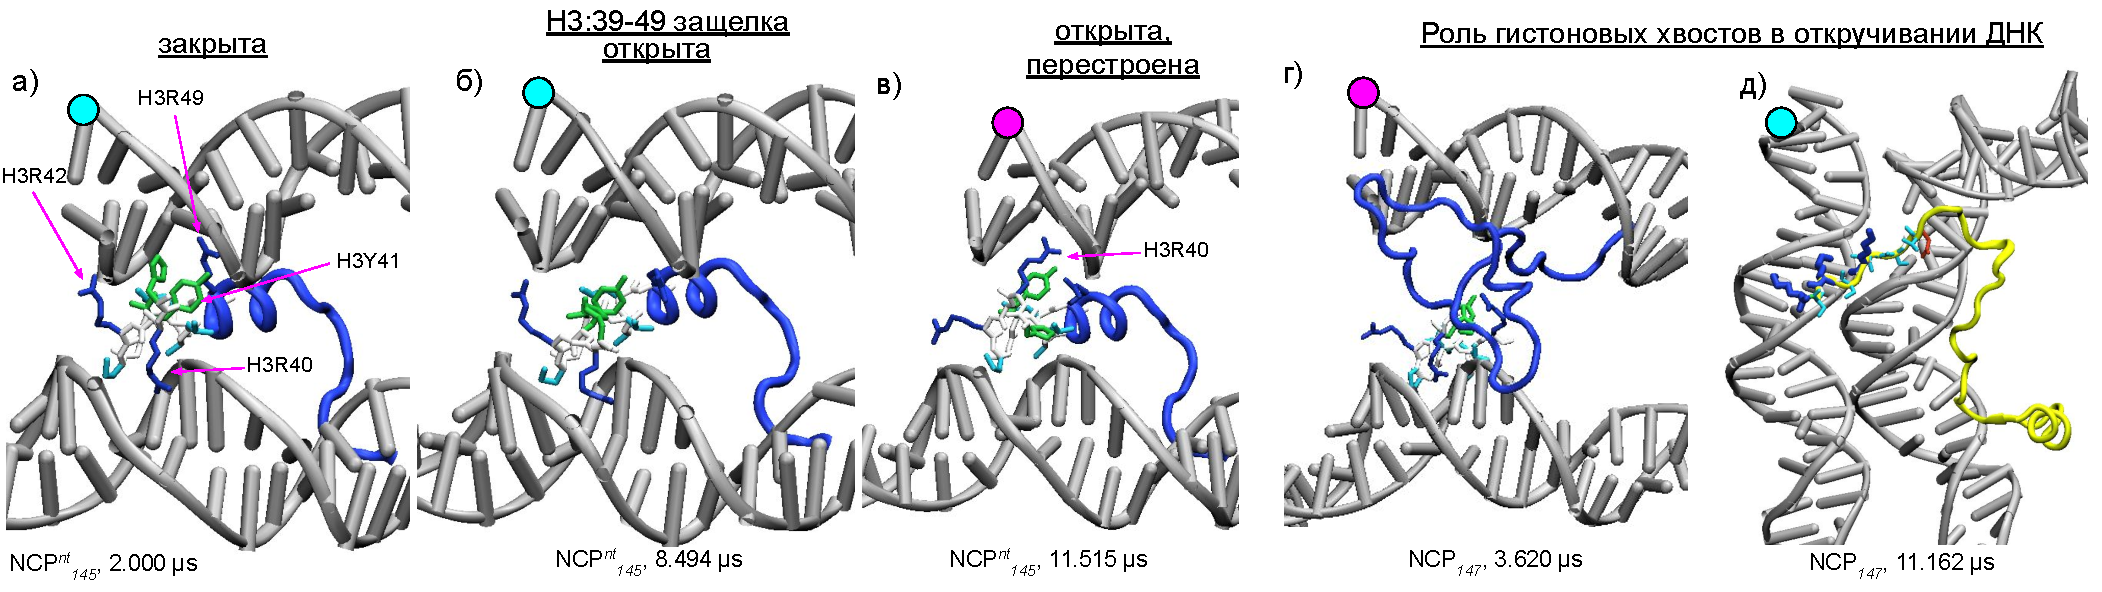
\includegraphics[width=\textwidth]{images/p2/10ms/fig3.pdf}
    \caption[Динамика ``защелки'' концов ДНК фрагментом гистона H3]{Динамика ``защелки'' концов ДНК фрагментом гистона H3}
    \label{fig:p2_3:f3}
\end{figure}



Каковым может быть функциональное значение отворачивания ДНК концов от гистонового кора? С одной стороны предполагается, что отворачивание ДНК необходимо для связывания различных факторов транскрипции \cite{li_rapid_2005}. В нашем моделировании для системы с гистоновыми хвостами ДНК не достигала такой степени отворота. Однако плотное взаимодействие хвостов с ДНК скорее всего распространится и на более существенные степени отворота ДНК. Таким образом, мы предполагаем, что важным фактором для определения доступности ДНК для транскрипционных факторов будет не только отворот ДНК, но и взаимодействия ДНК с гистоновыми хвостами. Другим возможным эффектом отворачивания ДНК является влияние изменение конформации нуклеосомальной ДНК на возможную укладку нуклеосом на супрануклеосомном уровне. Для оценки данных эффектов мы провели моделирование, в котором генерировали фибриллы из 10 нуклеосом, соединяя прямыми отрезками линкерной ДНК длиной 17 п.н. случайно выбранные  кадры из траекторий. Таким образом, можно было получить ансамбль конформаций нуклеосомных фибрилл и оценить распределение длин между концами фибрилл (Рис. \ref{fig:p2_3:f4}). По сравнению с фибриллами построенными на основе кристаллической структуры, фибриллы построенные с учетом флуктуаций концов коровой ДНК демонстрировали в среднем расстояние между концами на 10-15 нм больше. Ширина самого распределения составляла около 20 \AA. Таким образом, можно сделать вывод о том, что динамика концов ДНК, во-первых, ``разрыхляет'' супрануклеосомную структуру хроматина, а, во-вторых, обеспечивает достаточную конформационную гибкость фибриллы в пределах тепловых колебаний ($\sim$kT). 



\begin{figure}[H]
    \centering
    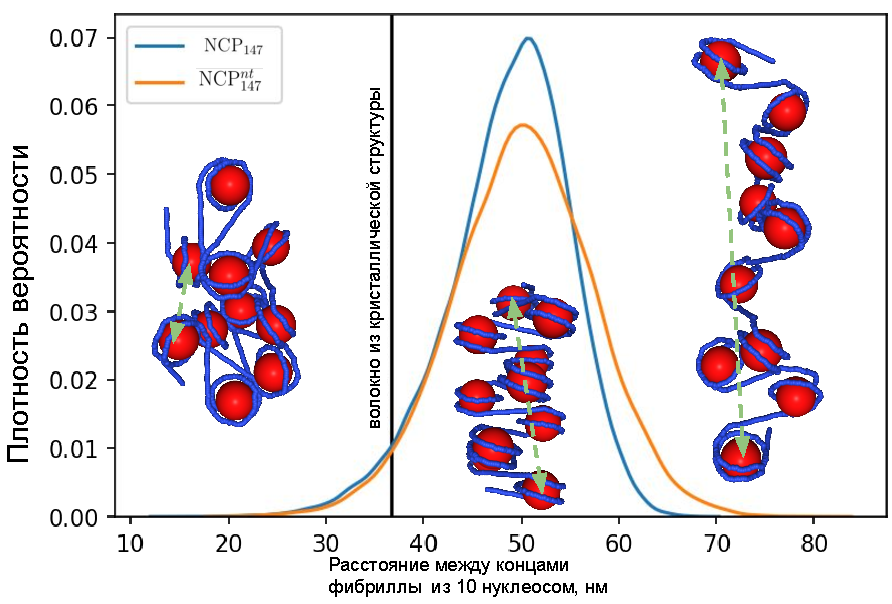
\includegraphics[width=\textwidth]{images/p2/10ms/fig4.pdf}
    \caption[Влияние динамики ДНК на структуру хроматиновых фибрилл]{Влияние динамики ДНК на структуру хроматиновых фибрилл}
    \label{fig:p2_3:f4}
\end{figure}


\subsubsection{Динамика кручения ДНК в нуклеосоме}

Интересным фактом в ходе моделирования явилось наблюдение релаксации дефекта кручения ДНК внутри нуклеосомного кора в системе NCP$_{147}^{nt}$. Дефект кручения ДНК в этой системе, основанной на 601-ой последовательности ДНК, располагается в районе SHL $\pm$5. По сравнению с нуклеосомами на основе альфа-сателлитной ДНК, ДНК в районе этого положения растянута на 1 нуклеотид, при этом совершает то же самое количество оборотов (см. рисунок \ref{fig:p2_3:f5}г). В ходе моделирования мы наблюдали резкий перескок регистра ДНК из кристаллоподобного состояния (Рис. \ref{fig:p2_3:f5}б) в состояние, где нуклеотиды начиная с нуклеотида номер -54 сместились в сторону диады нуклеосомы. Рисунок  \ref{fig:p2_3:f5}д иллюстрирует то, что данный сдвиг регистра ДНК далее произошел для всего конца ДНК, начиная приблизительно с нуклеотида -50. Таким образом около 20 нуклеотидов с проксимального конца ДНК испытали вращательное движение внутри нуклеосомного кора. Любопытным является изучение деталей данного механизма. Рассмотрение динамики отворачивание ДНК свидетельствует о том, что релаксация дефекта кручения произошла в области, которая не была затронута отворотом ДНК (Рис. \ref{fig:p2_3:f2}а). В то же время нельзя исключить, что отворот концов ДНК способствовал релаксации дефекта и его распространению вдоль ДНК. С точки зрения стальных контактов в системе NCP$_{145}^{nt}$ в районе SHL -6 в течение первой микросекунды моделирования наблюдался стабильный контакт нижней цепи ДНК в положении -58 с H2AT76 и верхней цепи ДНК в положении -54 с H2BS56. При анализе 10 микросекунды моделирования на предмет стабильных контактов между нуклеотидами и аминокислотами оказалось, что первый контакт остался неизменным, а второй контакт сместился на нуклеотид за номером -55. Таким образом, релаксация данного дефекта кручения была в некотором роде асимметрична. В большей степени наблюдалось сдвиг регистра контактов для верхней цепи ДНК. Интересным фактом является то, что как недавно было показано в структурных работах по изучению механизмов работ ремоделеров нуклеосом семейства ISWI и SWI/SNF, именно, верхняя цепь ДНК изменяет свое положение на нуклеосомном коре в первую очередь при связывании АТФ субъединицы ремоделера \cite{li_mechanism_2019}.

Еще одним интересным фактом сопровождающим релаксацию дефекта кручения ДНК в районе SHL -5 является деформация в этот момент спирали $\alpha2$ H2A гистона с отгибом ее С-конца в сторону центра нуклеосомного кора. С-конец данной спирали связан с сайтом связывания ДНК в районе SHL -5.5 и, вероятно, участвует в ослаблении контактов ДНК с гистоновым кором, которое помогает релаксации дефекта кручения.


\begin{figure}[H]
    \centering
    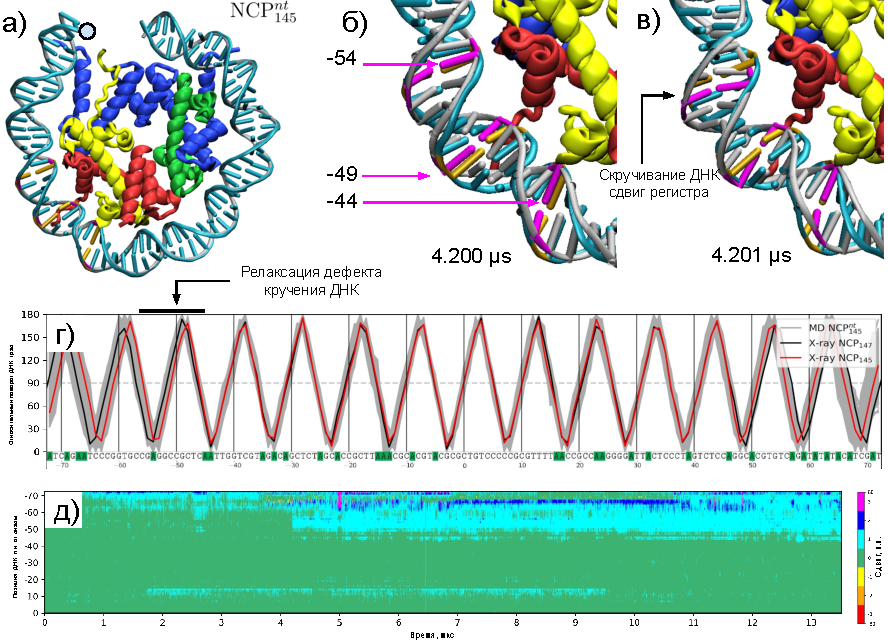
\includegraphics[width=\textwidth]{images/p2/10ms/fig5.pdf}
    \caption[Динамика кручения ДНК в нуклеосоме]{Динамика кручения ДНК в нуклеосоме. а) Структура проксимального супервитка нуклеосомы в начальный момент. Кристаллическая форма ДНК изображена голубым цветом, серым цветом ДНК в ходе МД моделирования. Оранжевым цветом отмечены пары нуклеотидов, которые участвуют изменяют положение на нуклеосоме. б) Кадр траектории до прокручивания ДНК. в) Кадр траектории после прокручивания ДНК. г) График параметра относительного кручения (relative twist) ДНК на нуклеосоме. д) Иллюстрация сдвига в положении нуклеотидов для верхней цепи ДНК относительно положения в кристаллической структуре.}
    \label{fig:p2_3:f5}
\end{figure}



\subsubsection{Динамика контактов ДНК-белок в нуклеосоме}

Наличие траекторий молекулярной динамики позволяет достаточно точно описать взаимодействия гистонов с ДНК на уровне контактов отдельных атомов, аминокислот, нуклеотидов. Причем в отличие от анализа кристаллических структуру имеется возможность оценить устойчивость и динамическую подвижность тех или иных контактов. Нами был проведен анализ стабильных контактов между аминокислотными остатками гистонов и нуклеотидами ДНК. Для изначального анализа была выбрана система NCP$_{147}$ в течение первой микросекунды моделирования, когда отворота ДНК не наблюдалась. Также поскольку система является псевдосимметричной мы учитывали только те контакты, которые присутствовали с обеих сторон нуклеосомы. Результат анализа приведена на рисунке \ref{fig:p2_3:f6}. Данные график иллюстрирует все основные особенности связывания ДНК с гистонами. Обратим внимание на две особенности, которые по нашему мнению имеют функциональное значение. Количество контактов, которые образует верхняя цепь ДНК значительно меньше, контактов которые образует нижняя цепь ДНК. Предполагаем, что это как раз может иметь значение при передвижении нуклеосом вдоль ДНК АТФ-зависимыми ремоделерами, которые как было показано недавно в первую очередь вытягивают и деформируют верхнюю цепь ДНК. Второй интересный момент связан с наличием области H3 гистона, которую мы называем ``защелкой'', которая взаимодействует как с концом коровой ДНК, так и с областью вблизи диады - около положения -9. Отметим, что вблизи положения -9 в геномных исследованиях по позиционированию нуклеосом наблюдается необычный сигнал - там чаще встречаются нуклеотиды A/T, хотя по общему правилу нуклеосомы предпочитают в области изгиба ДНК в сторону большой бороздки нуклеотиды G/C \cite{davey_does_2013}. Данные факт может отчасти объясняться плотным взаимодействием H3R40 внутри малой бороздки ДНК с электроотрицательным группами A/T оснований.


\begin{figure} [H]
    \centering
    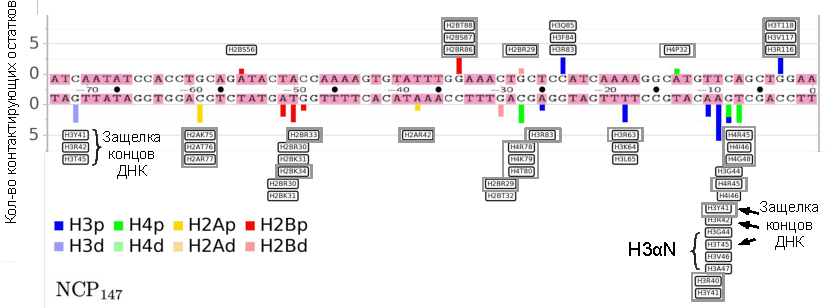
\includegraphics[width=\textwidth]{images/p2/10ms/fig6.pdf}
    \caption[Стабильные контакты ДНК-гистоны в нуклеосоме]{Стабильные контакты ДНК-гистоны в нуклеосоме. Отмечены контакты между нуклеотидами и аминокислотными остатками, присутствующие в 90\% кадров в системе NCP$_{147}$ в течение первой микросекунды моделирования с обоих симметричных сторон нуклеосомы. В рамках отмечены контакты, которые сохраняются с обоих сторон нуклеосомы в течение всей МД траектории.}
    \label{fig:p2_3:f6}
\end{figure}

\subsubsection{Пластичность гистонового октамера}

Как было описано во введении весьма актуальной темой научных исследований на данный момент является изучение пластичности октамера гистонов. Для исследования данного вопроса нами были построены проекции координат атомов $\alpha 2$-спиралей гистонов на плоскость нуклеосомного диска (Рис. \ref{fig:p2_3:f7}. Видно, что спирали испытывают флуктуации в пределах от нескольких до 5-6\AA. Особенно выделяются флуктуации концов C-концов спиралей гистона H2A. Недавно методами крио-ЭМ был разрешен ряд деформированных структур нуклеосомного кора, в частности структура нуклеосомы сжатая вдоль диадной оси на несколько процентов. RMSD кадров  МД траектории относительно данной структуры (Рис. \ref{fig:p2_3:f7}в) показывает, что данная структура зачастую отличается от кадров траектории не более, чем начальная структура самой траектории. Таким образом, можно сделать вывод, что наблюдаемые в эксперименте деформированные состояния нуклеосом находятся, по крайней мере, в рамках отличий, которые мы видим между кадрами траектории на масштабе мультимикросекундного моделирования.

В ряде работ было показано, что дисульфидные сшивки внутри димеров гистонов приводят к изменению функционирования нуклеосом. В частности H3L82C-H4V81C уменьшает термическую диффузию нуклеосом по ДНК и влияет на работу ремоделера SNF2h \cite{bilokapic_histone_2018,bilokapic_structural_2018,sinha_distortion_2017}. Расстояние между С-$\alpha$ атомами данные остатков изображена на рисунке \ref{fig:p2_3:f7}г. Оно колеблется в пределах от 6,1-8,5\AA. Длина дисульфидной связи составляет около 2,05\AA, расстояние между С-$\alpha$-атомом и атомом серы в стандартной конформации цистеина составляет 2,81\AA и не меняется при вращении торсионных углов. Таким образом максимальное расстояния между С-$\alpha$-атомами у остатков цистеина, связанных дисульфидной связью, составляет 7,67\AA. Следуя данным расчетам, видим, что дисульфидная сшивка будет препятствовать некоторым конформациям, наблюдаемым в динамике.

Для того, чтобы дополнительно изучить влияние пластичности октамера на динамику ДНК, мы провели расчеты, в которых $\alpha 2$-спирали гистонов были зафиксированы. Анализ флуктуационной динамики ДНК показал (см. рисунок \ref{fig:p2_3:f7}е), что у системы с фиксированными $\alpha$-спиралями подвижность ДНК была снижена на всем ее протяжении. Данные эффект требует дальнейшего изучения, однако можно предположить, что уменьшение подвижности ДНК отрицательно сказывается на возможности ремоделирования и скольжения нуклеосом.



\begin{figure} [H]
    \centering
    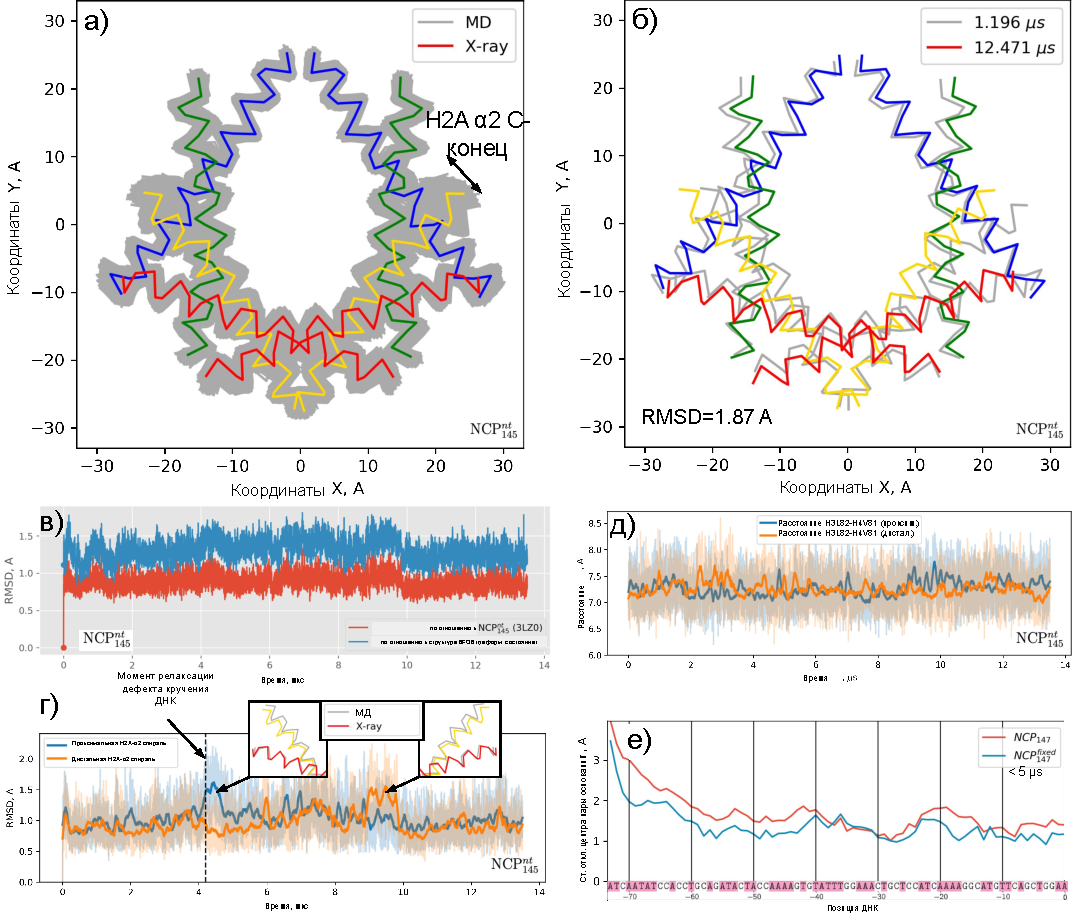
\includegraphics[width=\textwidth]{images/p2/10ms/fig7.pdf}
    \caption[Пластичность гистонового октамера]{Пластичность гистонового октамера. а) Наложение проекций координат С$\alpha$-атомов $\alpha 2$-спиралей гистонов в плоскости нуклеосомального диска из кадров МД траектории. б) Аналогичные проекции координат С$\alpha$-атомов для двух кадров с максимально различным RMSD. в) RMSD $\alpha 2$-спиралей гистонов в ходе МД относительно исходной структуры и структуры 6FQ6, полученной крио-ЭМ, с деформированной конформацией ядра нуклеосомы. г) Эволюция RMSD спирали $\alpha 2$ гистона H2A. д) Расстояние между остатками, которые подвергаются дисульфидным сшивкам в ряде экспериментов. e) Сравнение флуктуаций пар оснований ДНК в системах с закрепленными и незакрепленными $\alpha 2$-спиралями гистонов.}
    \label{fig:p2_3:f7}
\end{figure}

\subsubsection{Аллостерическая связь откручивания ДНК и конформации ДНК около диады}

Область ``застежки'' гистона H3 взаимодействует одновременно с двумя супервитками ДНК. Это наблюдение известно достаточно давно. Например, Horn et al. в своих экспериментах наблюдали, что SIN мутация гистона H4R25C взаимодействующая в положении SHL $\pm$0.5 приводит к ухудшению возможности компактизации нуклеосомальных фибрилл. Они предположили, что одним из возможных механизмов является дестабилизации концов нуклеосомальной ДНК в виду коммуникации области SHL $\pm$0.5 с областями SHL $\pm$6.5 посредством H3 $\alpha$N-спирали. Однако, Flaus et al. предположили, что этот эффект может объясняться увеличением мобильности нуклеосом и их смещению относительно исходных позиций \cite{flaus_sin_2004}. Тем не менее, нам было интересно рассмотреть в нашем моделировании возможные эффекты коммуникации областей SHL $\pm$0.5 и SHL $\pm$6.5. На рисунке \ref{fig:p2_3:f9} приведен сравнительных анализ откручивания ДНК и деформации ДНК в различных положениях от времени для системы NCP$_{147}$. Любопытным является факт, что вслед за откручиванием ДНК, зачастую область ``защелки'' гистона H3 теряет свои контакты не только с концом ДНК, но и с областью нижнего супервитка.
Такой случай изображен на панели \ref{fig:p2_3:f9}в. Потеря контактов с нижним супервитком ДНК в свою очередь ведет к деформации ДНК в этой области и к ее усиленным флуктуациям. Можно предположить, что наличие флуктуация в нижнем супервитке будет способствовать прохождению через нуклеосому дефектов скручивания ДНК.

В результате анализа приведенного в данном разделе нами выдвигается предположение о наличие динамической (аллостерической) связи между откручиванием ДНК и скольжению нуклеосом вдоль ДНК по механизму продвижения дефектов кручения. Откручивание концов коровой ДНК, во-первых, помогает образованию и прохождению дефектов скручивания вблизи концов ДНК, а, во-вторых, способствует дестабилизации ДНК в районе диады, что также, вероятно, помогает прохождению дефектов скручивания далее через нуклеосомную ДНК.



\begin{figure} [H]
    \centering
    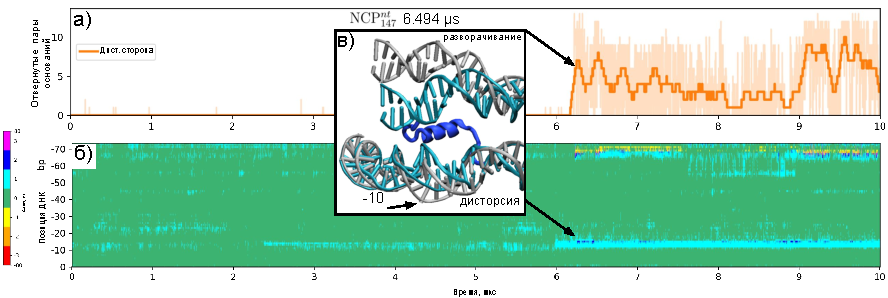
\includegraphics[width=\textwidth]{images/p2/10ms/fig9.pdf}
    \caption[Аллостерическая связь откручивания ДНК и конформации ДНК около диады]{Аллостерическая связь откручивания ДНК и конформации ДНК около диады. а) График откручивание ДНК от времени в ходе МД моделирования. б) График смещения нуклеотидов относительно кристаллической структуры.}
    \label{fig:p2_3:f9}
\end{figure}





\subsection{Благодарности}

Работа данного раздела поддержана грантами Российского научного фонда № 18-74-10006 (атомистическое моделирование нуклеосом и разработка и анализ траекторий нуклеосом), грантами Российского фонда фундаментальных исследований № 20-34-70039 (моделирование структуры супрануклеосомальных фибрилл) и № 19-34-51053 (метода анализа взаимодействий белков и нуклеиновых кислот). Исследования проводились на оборудовании коллективных исследовательских установок вычислительных ресурсов высокопроизводительных вычислений МГУ им. М.В. Ломоносова.


\section{Выводы главы \ref{part2_supermd}}
В данной главе на примере моделирования нуклеосом продемонстрированы возможности современных технологий суперкомпьютерного моделирования динамики биомакромолекулярных систем в атомистическом приближении на микросекундных временных масштабах. Проанализирована конформационная подвижность как коровых частиц нуклеосом (октамер гистонов + 147 пар нуклеотидов ДНК), так и нуклеосом с линкерной ДНК (октамер гистонов + 187 пар нуклеотидов ДНК). Изучена динамика хвостов и внутренняя подвижность глобулярных доменов гистонов, связь динамики белка и ДНК. Впервые в равновесной молекулярной динамике наблюдалась частичная диссоциация и реассоциация (отворот) ДНК от белкового октамера, изменение ориентационного положения ДНК, выпячивание ДНК вблизи входа-выхода в нуклеосому. На основании моделирования могут быть сформулированы следующие научные выводы и гипотезы:

\begin{itemize}
    \item Электростатическое отталкивание двух сегментов линкерной ДНК является одним из факторов, которые влияют на конформацию ДНК и углы входа-выхода ДНК из ядра нуклеосомы.
    \item В процессе спонтанного ступенчатого откручивания/прикручивания ДНК в нуклеосоме последовательно теряются стабильные взаимодействия ДНК с гистонами. Конформация ДНК подвержена значительным флуктуациям в наносекундном диапазоне. В переходе нуклеосом из кристаллоподобного состояния в состояние с отвернутой ДНК ключевую роль играют взаимодействия остатков гистона H3 между двумя супервитками ДНК.
   % \item Показано, что спонтанное откручивание ДНК от нуклеосомы приводит к разрыхлению структуры хроматиновых фибрилл.
    \item Формирование дефектов кручения ДНК в нуклеосоме и конформационные перестройки внутри глобулярных частей гистонового октамера, происходящие на микросекундных временах, указывают на возможность скольжения нуклеосом вдоль ДНК по винтовому механизму и транслокацию ДНК вдоль октамера.
    \item Диссоциации концов нуклеосомальной ДНК от гистонового октамера наблюдается на временах порядка 10 мкс. 
  %  \item Гистоновые хвосты в нуклеосоме активно взаимодействуют с коровой и линкерной ДНК, влияют на кооперативность взаимодействия белков хроматина с гистоновыми хвостами.
  %  \item Конформационные перестройки внутри глобулярных частей гистонового октамера, происходящие на микросекундных временах, влияют на подвижность ДНК и, вероятно, эффективность транслокации ДНК вдоль октамера.
   % \item Показано наличие аллостерических эффектов между откручиванием концов ДНК в нуклеосоме и стабильности центральной части ДНК, важные с точки зрения передвижения нуклеосом вдоль ДНК.  

\end{itemize}




%\begin{itemize}
 %   \item  Конформация линкерной ДНК в нуклеосомах подвержена значительным флуктуациям, которые влияют на углы входа-выхода ДНК из ядра нуклеосомы, электростатическое отталкивание двух сегментов линкерной ДНК является одним из факторов, влияющих на их конформацию и углы входа-выхода.
 %   \item Процесс спонтанного откручивания/прикручивания ДНК в нуклеосоме является ступенчатым процессом и характеризуется переходом между набором динамических состояний, в которых ДНК последовательно теряет стабильные взаимодействия с гистонами, но при этом ее конформация подвержена значительным флуктуациям в наносекундном диапазоне. Предложена структурно-кинетическая модель перехода нуклеосом из кристаллоподобного состояния в состояние с отвернутой ДНК, ключевую роль в которой играют взаимодействия остатков гистона H3, находящиеся между двумя супервитками ДНК.
 %   \item Показано, что спонтанное откручивание ДНК от нуклеосомы приводит к разрыхлению структуры хроматиновых фибрилл.
 %   \item Формирование дефектов кручения ДНК в нуклеосоме может происходить на микросекундных временных диапазонах, что указывает на возможность скольжения нуклеосом вдоль ДНК по винтовому механизму.
   % \item Гистоновые хвосты в нуклеосоме активно взаимодействуют с коровой и линкерной ДНК, влияют на кооперативность взаимодействия белков хроматина с гистоновыми хвостами.
   % \item Конформационные перестройки внутри глобулярных частей гистонового октамера, происходящие на микросекундных временах, влияют на подвижность ДНК и, вероятно, эффективность транслокации ДНК вдоль октамера.
   % \item Показано наличие аллостерических эффектов между откручиванием концов ДНК в нуклеосоме и стабильности центральной части ДНК, важные с точки зрения передвижения нуклеосом вдоль ДНК.  
%\end{itemize}
 


% \subsection{Положения выносимые на защиту}
% %положения выносимые на защиту
% \begin{enumerate}
%   \item На примере нуклеосом разработаны подходы атомистического суперкомпьютерного моделирования биомакромолекулярных комплексов белков и нуклеиновых кислот, способные описывать и анализировать функциональную динамику молекул в микросекундных временных диапазонах.
%   \item С использованием данных подходов охарактеризована на атомистическом уровне функциональная динамика нуклеосом, важная с точки зрения эпигенетической регуляции функционирования генома, охарактеризованы новые моды динамической подвижности, связанные с частичной диссоциацией ДНК от гистонового октамера, перестройкой взаимодействий гистоновых хвостов, деформацией глобулярных доменов гистонов.
% \end{enumerate}           % Глава 2 - Методы МД в исследовании нуклеосом (во введение упомянуть про HistoneDB. Разделы - описание объекта и провлемы , описание методов)
%\chapter{Расчет свободной энергии гидратации и адсорбции аминокислот} \label{part3_free_energy}


Данная глава иллюстрирует подходы молекулярного моделирования, позволяющие вычислять экспериментально измеримые термодинамические характеристики на основе молекулярно-динамических атомистических моделей.
В главе речь пойдёт об изучении гидратации боковых цепей аминокислот вблизи поверхности воды путём построения профилей свободной энергии на основании классических атомистических моделей молекул. Работа также имеет методологическое значение, поскольку в ней впервые предприняты попытки высокоточной численной оценки термодинамических параметров гидратации и адсорбции. Материалы данной главы следуют изложению приведенному в кандидатской депортации автора \cite{shaytan_thesis_kfmn_2010}, основаны на следующих статьях \cite{shaytan_free_2010,shaytan_solvent_2009} и материалах конференций \cite{shaytan_peptide_2006}. 

\graphicspath{{images/p3/}}

\section{Введение}
Применение молекулярной динамики к анализу поверхностных явлений нашло широкое применение за последние 20 лет поскольку позволяет дополнять экспериментальные данные и получать новой информацию на молекулярном уровне ~\cite{rev_benjamin_liq-liq_interf_1997,rev_pohorille_model_aq_sol_interf_2002}.
Величины, которые зачастую интересуют исследователя имеют статистическую природу (например, энергии связывания, коэффициенты распределения и т.д.), вычисление таких величин в компьютерном эксперименте требует серьёзной статистической выборки и значительных вычислительных ресурсов, одновременно накладывая ограничения на размеры и сложность молекулярных систем.

Методология вычисления свободных энегий (особенно с использованием стандартных силовых полей для белковых сруктур) получила много внимания за последнее десятилетие \cite{chipot_2002}, многие работы были посвящены систематической и критической оценке и сравнению методово, силовых полей, протоколов молекулярной динамики \cite{fee_maccalum_2003,fee_villa_2002,bar_comp,comp_fe_meth_2006,fee_hess_2006,fee_mobley_2007,shirts_waterff,shirts_proteinff,shirts_theory}. Однако эти работы в основном сводились к расчёту параметров в гомогенных системах (например, расчёту свободной энергии сольватации небольших молекул), в основном в воде, и в них не затрагивались вопросы расчёта систем с границей раздела фаз. Так было определено, что энергии гидратации боковых цепей аминокислот рассчитанные методом МД находятся в хорошей
 корреляции с экспериментальными данными, но систематически завышены. Разумным продолжением ряда этих работ является рассмотрение взаимодействия таких молекул не только с объёмом растворителя, но и с его границей. Если говорить о высокоточных оценках свободной энергии, то речь можно вести о достижении точности серьёзно выше $2 - 4$ кДж/моль, что является пределом точности, например, при предсказании связывания лигандов и белков при разработке лекарств. Если речь идёт не о качественных, а о количественных предсказаниях, то необходимая точность порядка 1 кДж/моль. Если же говорить, о настройке силовых полей на базе этих данных, то желаемая точность может быть около 0.1 кДж/моль.

\section{Постановка задачи}
Задачей данного исследования явился расчёт профилей свободной энергии для соединений аналогов нейтральных боковых цепей аминокислот на границе вода/пар с высокой точностью, вычисление энергий гидратации и адсорбции. В данной работе мы попытались обобщить и разработать наиболее точные и проверенные технологии таких расчётов, чтобы исключить зависимость результатов от методики расчётов. Для оценки качества результатов был проведён отдельный расчёт энергий гидратации молекул в объёме с использованием алгоритма Беннетта (Bennett acceptance ratio algorithm).
Для изучения были выбраны широко используемые модели соединений в силовом поле OPLS-AA \cite{opls-aa} с моделью воды  SPC.



\section{Teоретические аспекты расчета свободной энергии на границе фаз}
\subsection{Профиль плотности границы раздела вода-пар}

Профиль плотности границы раздела вода-пар удовлетворительно описывается полу-феноменологической капиллярно-волновой теорией (КВТ). Согласно КВТ \cite{cwt_stillinger_1965,rev_benjamin_liq-liq_interf_1997} профиль плотности может быть описан как некоторый молекулярный профиль, уширенный термическими капиллярными волнами. Экспериментальные результаты и результаты моделирования \cite{rev_surf_struct_penfold_2001,cap-simul_senapati_2001, int-wat-polar_rivera_2006} допускают, что толщина границы раздела зачастую может быть описана только капиллярными волнами, то есть является практически ступенчатой на молекулярном уровне. В этом случае профиль плотности может быть описан функцией интеграла ошибок:
\begin{equation}
\rho_z=\frac{1}{2}(\rho_L+\rho_V)-\frac{1}{2}(\rho_L-\rho_V)\mathrm{erfc}\left[\frac{(z-z_0)}{\sigma \sqrt{2}}\right]
\label{erf_prof}
\end{equation}
где $\rho_L$ и $\rho_V$ плотность жидкости и пара, а $\sigma$ толщина границы раздела.

Известной проблемой при моделировании границ раздела является зависимость толщины границы от линейных размеров поверхности $L_x$. Согласно КВТ имеется логарифмическая зависимость толщины от линейного размера (из-за зависимости от размера количества возможный волновых мод):
\begin{equation}
\sigma^2=\frac{k_BT}{2\pi\gamma}\ln{\left(\frac{L_{||}}{B_0}\right)}
\label{cap_wave_dep}
\end{equation}
где $\gamma$ поверхностное натяжение, $B_0$ характерная длина коротковолновой обрезки спектра, обычно полагаемая равной размеру молекулы.

В термодинамическом пределе (без учёта гравитации) толщина границы плоского раздела фаз - расходится для жидкостей только с взаимодействиями ближнего порядка при рассмотрении в трёх и менее измерениях \cite{nointin3d_robert_1985}.

\subsection{\label{pmf_theor_backgr}Теория профилей свободной энергии}

На рис. \ref{system} представлена геометрия двухфазной системы с плоской границей раздела, которая перпендикулярна оси Z. В системе присутствует вода, пар и тестовая молекула S, для которой мы хотим посчитать её профиль свободной энергии вдоль оси Z.
Система находится при постоянной температуре и давлении (за счёт хорошей сжимаемости пара). Предположим, что система описывается в классическом приближении, тогда система из N частиц описывается своей функцией потенциальной энергии  ~\cite{landau_tm} $U(\vec{q})$, зависящей от 3N обобщённых координат  $\vec{q}$. Чтобы отслеживать положение тестовой молекулы введём функцию $d_{z}(\vec{q})$, которая является проекцией расстояния между центрами масс тестовой молекулы и водного слоя на ось Z.
Основные формулы статистической физики \cite{stat_mech_book_2000},  которые нам нужны, это соотношения связывающие распределение вероятности, профили свободной энергии и потенциал средней силы.
В нашем случае вероятность найти молекулу S на расстоянии $z$ от центра масс водного слоя есть:
\begin{equation}
P(z)=<\delta(d_{z}-z)>=\frac{\int{\delta(d_{z}-z)e^{-U/kT}d\vec{q}}}{\int{e^{-U/kT}d\vec{q}}}
\label{probab}
\end{equation}
где $<...>$ усреднение по каноническому ансамблю, $k$ постоянная Больцмана, $T$ -температура. 

Зная распределение, мы можем рассчитать профиль свободной энергии:

\begin{equation}
W(z)=-kT\ln{P(z)}+F_0
\label{fe_prof}
\end{equation}

- где $F_0$ произвольная константа. В эксперименте профиль вероятности будет соответствовать профилю концентрации, предполагая, конечно, что раствор является разбавленным, или идеальным. Кирквуд~\cite{kirkwood} ввёл понятие потенциала средней силы (ПСС) и показал, что профиль потенциала средней силы с точностью до константы равен профилю свободной энергии. В нашем случае средней силой является средняя сила взаимодействия тестовой молекулы и водного слоя при условии, что проекция расстояния между центрами масс на ось Z фиксирована. Средняя сила задаётся как:
\begin{equation}
\overline{F(z)}=\frac{
 \int{<\delta(d_{z}(\vec{q})-z)>\nabla_{d_z}U(\vec{q})e^{-U/kT}d\vec{q}}
}
{\int{e^{-U/kT}d\vec{q}}}
\label{mf}
\end{equation}
где $\nabla_{d_z}$ оператор градиента, связанный с расстоянием вдоль оси Z между центрами масс.
Можно показать, что профиль свободной энергии и потенциал средней силы -- это одно и то же:

\begin{equation}
\frac{\partial W(z)}{\partial z}=\overline{F(z)}
\end{equation}

\subsection{\label{hfe_theor_backgr}К вопросу вычисления энергий гидратации}

В случае попарно-аддитивных молекулярных взаимодействий функцию потенциальной энергии можно разбить таким образом, чтобы выделить взаимодействие между тестовой молекулой и растворителем:
\begin{equation}
U(\vec{q},\lambda)=U_{wat}(\vec{q}_{wat})+\lambda U_{int}(\vec{q}_{wat},\vec{q}_{S})+U_S(\vec{q}_{S})
\label{pot_ener}
\end{equation}
\\
где $U_{wat}$,$U_{S}$,$U_{int}$, потенциальные энергии молекул воды, молекулы растворённого вещества и энергия их взаимодействия, соответственно.
Обобщённые координаты разбиваются удобным образом так, что $\vec{q_{S}}$ -- это координаты, описывающие конфигурацию молекулы S (молекулы растворённого вещества) в ящике с водой, $\vec{q}_{wat}$ -- координаты всех молекул воды.
$\lambda$ -- это параметр сопряжения, вводимый для последующих выкладок. При $\lambda=1$ и $\lambda=0$ взаимодействия между молекулой S и водой включены и отключены полностью, соответственно. 

Энергия гидратации, как показано в приложении -- это свободная энергия (работа) включения взаимодействий между молекулой S и остальным раствором в NPT ансамбле \cite{shaytan_free_2010}. 
Энергия гидратации Гиббса $\Delta G_{hydr}$ может быть выражена:
\begin{equation}
\Delta G_{hydr}=-kT \ln \left( \frac{\Delta (P,T,\lambda=1)}{\Delta (P,T,\lambda=0)} \right)
\label{hydr_fe_sim}
\end{equation}

где  $\Delta (P,T,\lambda)$ -- изотермо-изобарическая функция распределения вида:
\begin{equation}
\Delta (P,T,\lambda) \propto \frac{1}{N!}\int\int\int dPd\vec{q}\exp\left(-\left[U(\vec{q},\lambda)+PV\right]/kT\right)
\label{hydr_fe_expr}
\end{equation}
и N - число молекул воды. Такая формулировка верна в термодинамическом пределе  ($N\rightarrow\infty$) пока у нас есть одна молекула S.
Можно показать, что химический потенциал растворённого вещества (молекулы S) в идеальном растворе выражается как:
\begin{equation}
\mu_S=-kT\ln(1/c)+\Delta G_{hydr}
\label{chem_pot}
\end{equation}
где $c$ - концентрация растворённого вещества.

Таким образом с экспериментальной точки зрения свободная энергия гидратации может быть получена путём измерения концентрации вещества S в воде $c_{wat}$ и паре $c_{gas}$:
\begin{equation}
\Delta G_{hydr}^{exp}=kT\ln\left(\frac{c_{gas}}{c_{wat}}\right)
\label{hydr_energy_exp}
\end{equation}


\subsection{\label{ads_fe_theory}Энергии адсорбции}
Параметры, описывающие поверхностную активность веществ, обычно описываются в терминах теории адсорбции Гиббса (хотя есть и другие: Ван-дер-Ваальса, Кана-Хилларда). В теории Гиббса \cite{gibbs_ads_theory} поверхность раздела считается отдельной двумерной фазой, расположенной на поверхности раздела Гиббса (ПРГ), и характеризуется двумерными величинами концентрации, называемыми, избытками Гиббса $\Gamma^i$). Согласно Гиббсу, объёмные фазы характеризуются своими объёмными концентрациями вплоть до границы раздела, а любой избыток или недостаток вещества в районе границы раздела описывается соответствующими двумерными избытками Гиббса.
Зная профиль концентрации $c^i(z)$, а также величины концентрации в объёме $c^i_1$, $c^i_2$, избыток Гиббса может быть рассчитан по формуле:
\begin{equation}
\Gamma^i=\int_{-\infty}^{z_0}(c^i(z)-c^i_1)dz+\int_{z_0}^{\infty}(c^i(z)-c^i_2)dz
\label{excess}
\end{equation}
где $z_0$ - координата ПРД. Позиция ПРД обычно выбирается так, чтобы избыток Гиббса для растворителя был равен нулю.
В этих переменных можно записать уравнение адсорбции Гиббса, которое соотносит избыток Гиббса ($\Gamma^S$), концентрацию вещества в объёмной фазе ($c^S$) и поверхностное натяжение ($\gamma$):

\begin{equation}
\Gamma^S=-\frac{1}{kT}\frac{d\gamma}{d\ln{c^S}}
\label{GAE}
\end{equation}
Мерой поверхностной активности обчно считается отношение $\Gamma^S/c^S$ в пределе бесконечно разбавленного раствора ($c^S\rightarrow 0$).
Это отношение можно оценить путём измерения поверхностного натяжения при различных концентрациях, что следует из (\ref{GAE}):
\begin{equation}
\left. \frac{\Gamma^S}{c^S}  \right|_{c^S\rightarrow 0}=-\frac{1}{kT}\left. \frac{d\gamma}{dc^S} \right|_{c^S\rightarrow 0}
\label{exp_GE_conc_ratio}
\end{equation}
Понятие энергии адсорбции может быть далее введено, хотя оно остаётся до некоторой степени произвольно определённым, поскольку оно зависит от выбора стандартных состояний или толщины границы раздела (толщины поверхностного монослоя). Один из возможных вариантов состоит в определении величины толщины поверхностного слоя $\tau$, тогда энергию адсорбции можно записать в виде:
\begin{equation}
G_{ads}=-kT\ln{\frac{\Gamma^S}{c^S\tau}}
\label{ads_fe_eq}
\end{equation}
Однако при сравнении экспериментальных значений энергии всегда нужно обращать внимание на то, какому определению следовали экспериментаторы.




\section{Методы расчёта}
Для расчёта профилей использовался классический метод молекулярной динамики в комбинации с методом удерживающей силы для расчёта профилей свободной энергии. Для расчёта энергий гидратации в объёме использовался метод Беннетта. В данном разделе описывается модель силового поля, протоколы МД, а также методика расчёта. Более подробное описание нюансов протоколов и обоснование их выбора приведено в статье \cite{shaytan_free_2010}.

\subsection{\label{sec:forcefield}Силовое поле и модель}
Для создания модели было выбрано полноатомное силовое поле  OPLS-AA \cite{opls-aa}
и твёрдая (с фиксированными внутренними степенями свободы) модель воды SPC \cite{spc}. Основные характеристики модели воды представлены в таблице \ref{wat_param}. 
Атомы представляются как классические частицы, соединённые связями. Невалентные взаимодействия представлены потенциалами Леннард-Джонса и Кулона:
\begin{equation}
U^{nb}=\sum_{i<j}4\epsilon_{ij}\left[\left(\frac{\sigma_{ij}}{r_{ij}}\right)^{12}-\left(\frac{\sigma_{ij}}{r_{ij}}\right)^{6}\right]+\sum_{i<j}\frac{q_iq_j}{4\pi r_{ij}^2}
\label{non-bond}
\end{equation}
\begin{table}[p]

	\begin{tabular}{ccccccc}
$\sigma$, \AA & $\epsilon$, кДж/моль & $q_o$, $e$ & $q_h$, $e$ & $l_{OH}$, \AA & $\theta^{\circ}$ & P, D  \\
	\hline
3.166 & 0.65 & -0.82 & 0.41 & 1.0 & 109.47 & 2.27
\end{tabular}

	\caption{Основные характеристики модели воды SPC, включая параметры Леннард-Джонса $\sigma,\epsilon$, частичные заряды на кислороде ($q_o$) и водороде ($q_h$), длины связей, HOH угол ($\theta^{\circ}$) и дипольный момент ($P$).}
	\label{wat_param}
\vspace{2 in}
\end{table}
 

Валентные взаимодействия включали угловые, торсионные и ложно торсионные члены. 
Параметры потенциала Леннард-Джонса и заряды для соединений были взяты из работы \cite{shirts_proteinff}.
В таблице \ref{molecules} представлены 13 нейтральных аминокислот и соответствующие им соединения аналоги боковых цепей, которые изучались в данной работе.
\begin{table*}[p]

	\begin{tabularx}{\textwidth}{XXXX}
Аминокислота & Вещество аналог боковой цепи & Химическая формула & Сокр. обозначение \\
	\hline

аланин       & метан   					  & CH$_4$      						 &  ALA'  \\
валин     & пропан					    & C$_3$H$_8$ 							 &  VAL'  \\
лейцин & изобутан 					  & C$_4$H$_{10}$			 			 &  LEU'  \\
изолейцин    & н-бутан     					& C$_4$H$_{10}$						 &  ILE'  \\
цистеин   & метанэтиол 					& CH$_3$SH    						 &  CYS'  \\
метионин    & метилэтилсульфид  & C$_2$H$_5$SCH$_3$  			 &  MET'  \\
серин       & метанол				& CH$_3$OH        			   &  SER'  \\
треонин     & этанол								& C$_2$H$_5$OH      			 &  THR'  \\
тирозин& п-крезол						& C$_3$C$_6$H$_4$OH		 	   &  TYR'  \\
фенилаланин & толуол								& C$_6$H$_5$CH$_3$   			 &  PHE'  \\
триптофан    & 3-метилиндол 				& C$_6$H$_4$C$_2$HNHCH$_3$ &  TRP'  \\
аспарагин    & ацетамид					& CH$_3$CONH$_2$					 &  ASN'  \\
глутамин     & пропионамид					& C$_2$H$_5$CONH$_2$       &  GLN'  \\
\end{tabularx}
	
	\caption{Список 13 изученных нейтральных веществ - аналогов боковых цепей аминокислот, из названия, химические формулы и обозначения.}
	\label{molecules}

\end{table*}


\subsection{\label{sec:fep_method} Расчёт профилей свободной энергии}
Для расчёта профиля свободной энергии соединений на границе раздела фаз вода/пар была сконструирована модель границы раздела, см. Рис. \ref{system}. Прямоугольный слой воды толщиной 4 нм помещён в расчётную ячейку (3x3x20нм$^3$), чьи размеры постоянны в ходе моделирования. Количество молекул воды - 1173. Расчёты проводились в пакете GROMACS  v. 3.3.1 \cite{gromacs}. Для расчёта профиля свободной энергии использовался метод сдерживающей силы. С помощью алгоритма поддерживалась фиксированная проекция  расстояния между центрами масс молекулы и водного слоя на ось, перпендикулярную к поверхности. На каждом шаге измерялась сдерживающая сила, которую необходимо было прикладывать, чтобы это расстояние оставалось фиксированным. Для этого использовался, так называемый, GROMACS pull code, который поддерживал проекцию расстояния постоянной с использованием алгоритма SHAKE \cite{shake}. Исследуемая молекула помещалась на различных расстояниях от центра масс водного слоя, и для каждой такой системы после уравновешивания проводился расчёт длиной в 4 нс. Для каждой молекулы было рассчитано 80 точек: положение от -4 нм до 4 нм с шагом 0.1 нм. Мгновенная сила записывалась на каждом шаге, затем усреднялась. Профиль средней силы затем аппроксимировался кубическим сплайном, учитывая симметрию профиля относительно z=0 (см. Рис. \ref{4pmf}). Интегрированием профиля средней силы вычислялся профиль свободной энергии. Соответствующие теоретические формулы приведены в статье \cite{shaytan_free_2010}.

     
\begin{figure}
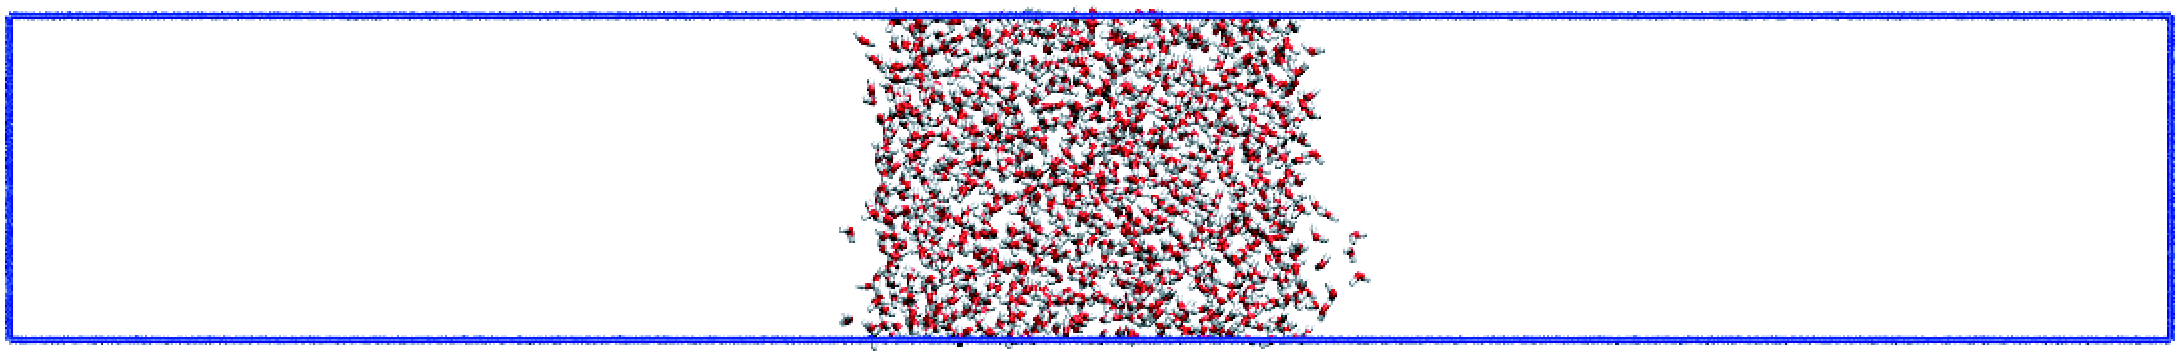
\includegraphics[width=17cm,height=2.5cm]{system}
\caption{\label{system} Мгновенное изображение модели системы с границей раздела вода/пар в периодической ячейке. Наиболее длинная сторона ячейки совпадает с нормалью к границе раздела (ось Z).}
\end{figure}


\subsection{\label{sec:hfe_method} Расчёт энергий гидратации}
Энергии гидратации рассчитывались по методу Беннетта \cite{bar} путём постепенного ``отключения'' взаимодействий между молекулой растворённого вещества и растворителем в ячейке, содержащей около 900 молекул воды.
Теоретические основы и детали метода Беннетта для оценок энергии гидратации могут быть найдены в работах других исследователей \cite{smith_bar,bar_comp,shirts_waterff}. Основные статистические соотношения приведены в статье \cite{shaytan_free_2010}.

Здесь мы приведём основные параметры нашего расчёта. Использовался стандартный термодинамический цикл: сначала молекула постепенно ``отключалась'' от среды путём зануления зарядов и параметров потенциала Леннард-Джонса, а затем проводился аналогичный коррекционный расчёт в вакууме, чтобы измерить поправку на внутримолекулярные взаимодействия. Отключение (мутация) молекулы в обоих случаях проводилась в 10 шагов. Сначала занулялись заряды, а потом отключались взаимодействия Леннар-Джонса. Электростатика отключалась в 2 шага, сначала заряды уменьшались в $\sqrt{2}$ раз, а затем занулялись. Взаимодействия Леннард-Джонса отключались в 8 шагов согласно формуле:
\begin{eqnarray}
U^{LJ}_{S}=\sum_{j}\sum_{i}f(i,j)\lambda4\epsilon_{ij}& & \nonumber \\
  \times\left(\frac{\sigma_{ij}^{12}} {(\alpha\sigma_{SC}^6(1-\lambda)+r_{ij}^6)^2}-\frac{\sigma_{ij}^6}{\alpha\sigma_{SC}^6(1-\lambda)+r_{ij}^6}\right) & &
\end{eqnarray} где $i$ поробегает по всем атомам растворённого вещества, $j$ по всем атомам в системе, $f(i,j)$ - ответственна за исключение взаимодействия между атомами связанными валентно. $\alpha=0.5,\sigma_{SC}=0.3\;нм$. В такой форме этапы мутации соответствовали параметрам $\lambda=1,0.8,0.7,0.6,0.5,0.4,0.3,0.2,0$. Для каждой стадии осуществлялись расчёты длиной 5 нс. Конфигурации записывались каждые 2 пс. Эти конфигурации обрабатывались по алгоритму Беннетта, чтобы получить оценку разницы свободной энергии между смежными состояниями.

\subsection{\label{sec:simprot}МД протокол}
В качестве алгоритма для получения выборок мы использовали динамику Ланжевена, согласно уравнению: 
\begin{equation}
m_i\frac{d^2\mathbf{r}_i}{dt^2}=-m_i\xi_i\frac{d\mathbf{r}_i}{dt}+\mathbf{F}_i(\mathbf{r}_i)+\hat{\mathbf{r}}_i
\label{langevin}
\end{equation}
где $\xi_i$ константа трения, а $\hat{\mathbf{r}}_i(t)$ шумовой процесс $<\hat{\mathbf{r}}_i(t)\hat{\mathbf{r}}_j(t+s)>=2m_i\xi_ikT\delta(s)\delta_{ij}$. Ланжевенова динамика является точным методом, позволяющим реализовать изотермический ансамбль.

Использовался пакет GROMACS  v 3.3.1 \cite{gromacs}, скомпилированный с двойной точностью. Уравнения Ланжевена интегрировались с исользованием лип-фрог алгоритма третьего порядка \cite{leap_frog_lang_gunsteren_1988} с шагом 2 фс. Для фиксации длин связей использовались алгоритмы  LINCS \cite{lincs} и SETTLE \cite{settle}. Расчёты проводились при постоянной температуре 300 К.
Константа трения $\xi$ для каждого атома рассчитывалась как $\xi_i=m_i/\tau_T$, где $\tau_T=1$ пс, $m_i$ -- масса атома. Для расчётов энергии гидратации использовался алгоритм задания изобарического ансамбля Паринелло-Рамана \cite{barostat} при 1 атм, время релаксации 2 пс, сжимаемость $4.5*10^{-5}$ бар$^{-1}$.  
Для расчёта электростатических взаимодействий использовался метод PME \cite{pme,pme2} с радиусом обрезки в прямом пространстве 1.3 нм и PME-порядком 6. Максимальное расстояние в пространстве фурье (maximum Fourier spacing) задовалось равным 0.12 нм.
Относительная толерантность между вкладами в энергию прямого и обратного пространств $10^{-5}$. Для потенциала Леннард-Джонса использовалась свитч функция, сглаживающая потенциал между 1.0 и 1.2 нм. Коррекционая поправка  (long-range correction) учитывалась при вычислении энергии и давления.

\section{Результаты и обсуждение}

\subsection{\label{sec:wat_res}Свойства водного слоя}
Чтобы оценить правильность нашей модели, рассмотрим сначала свойства модели границы раздела фаз. Расчёт длиной в 50 нс был проведён для того, чтобы оценить профиль плотности, поверхностный потенциал и ориентационное поведение молекул воды.
Профиль плотности идеально описывается уравнением \ref{erf_prof} с параметрами $ \sigma=0.14 $ нм,
 $ \rho_g=0.2 $ kg/m$^3$ и $ \rho_L=970.5 $ kg/m$^3$, поверхность раздела Гиббса находится в точках $z=\pm2.007$ нм. Толщина границы, рассчитанная из теории капиллярных волн  $\sigma_{CWT}=1.45$ \AA, хорошо согласуется с данными моделирования ($ \sigma=0.14 $ нм).

% \begin{equation}
% \rho_z=\frac{1}{2}(\rho_L+\rho_V)-\frac{1}{2}(\rho_L-\rho_V)\mathrm{erfc}\left[\frac{(z-z_0)}{\sigma \sqrt{2}}\right]
% \label{erf_prof}
% \end{equation}


\begin{figure}
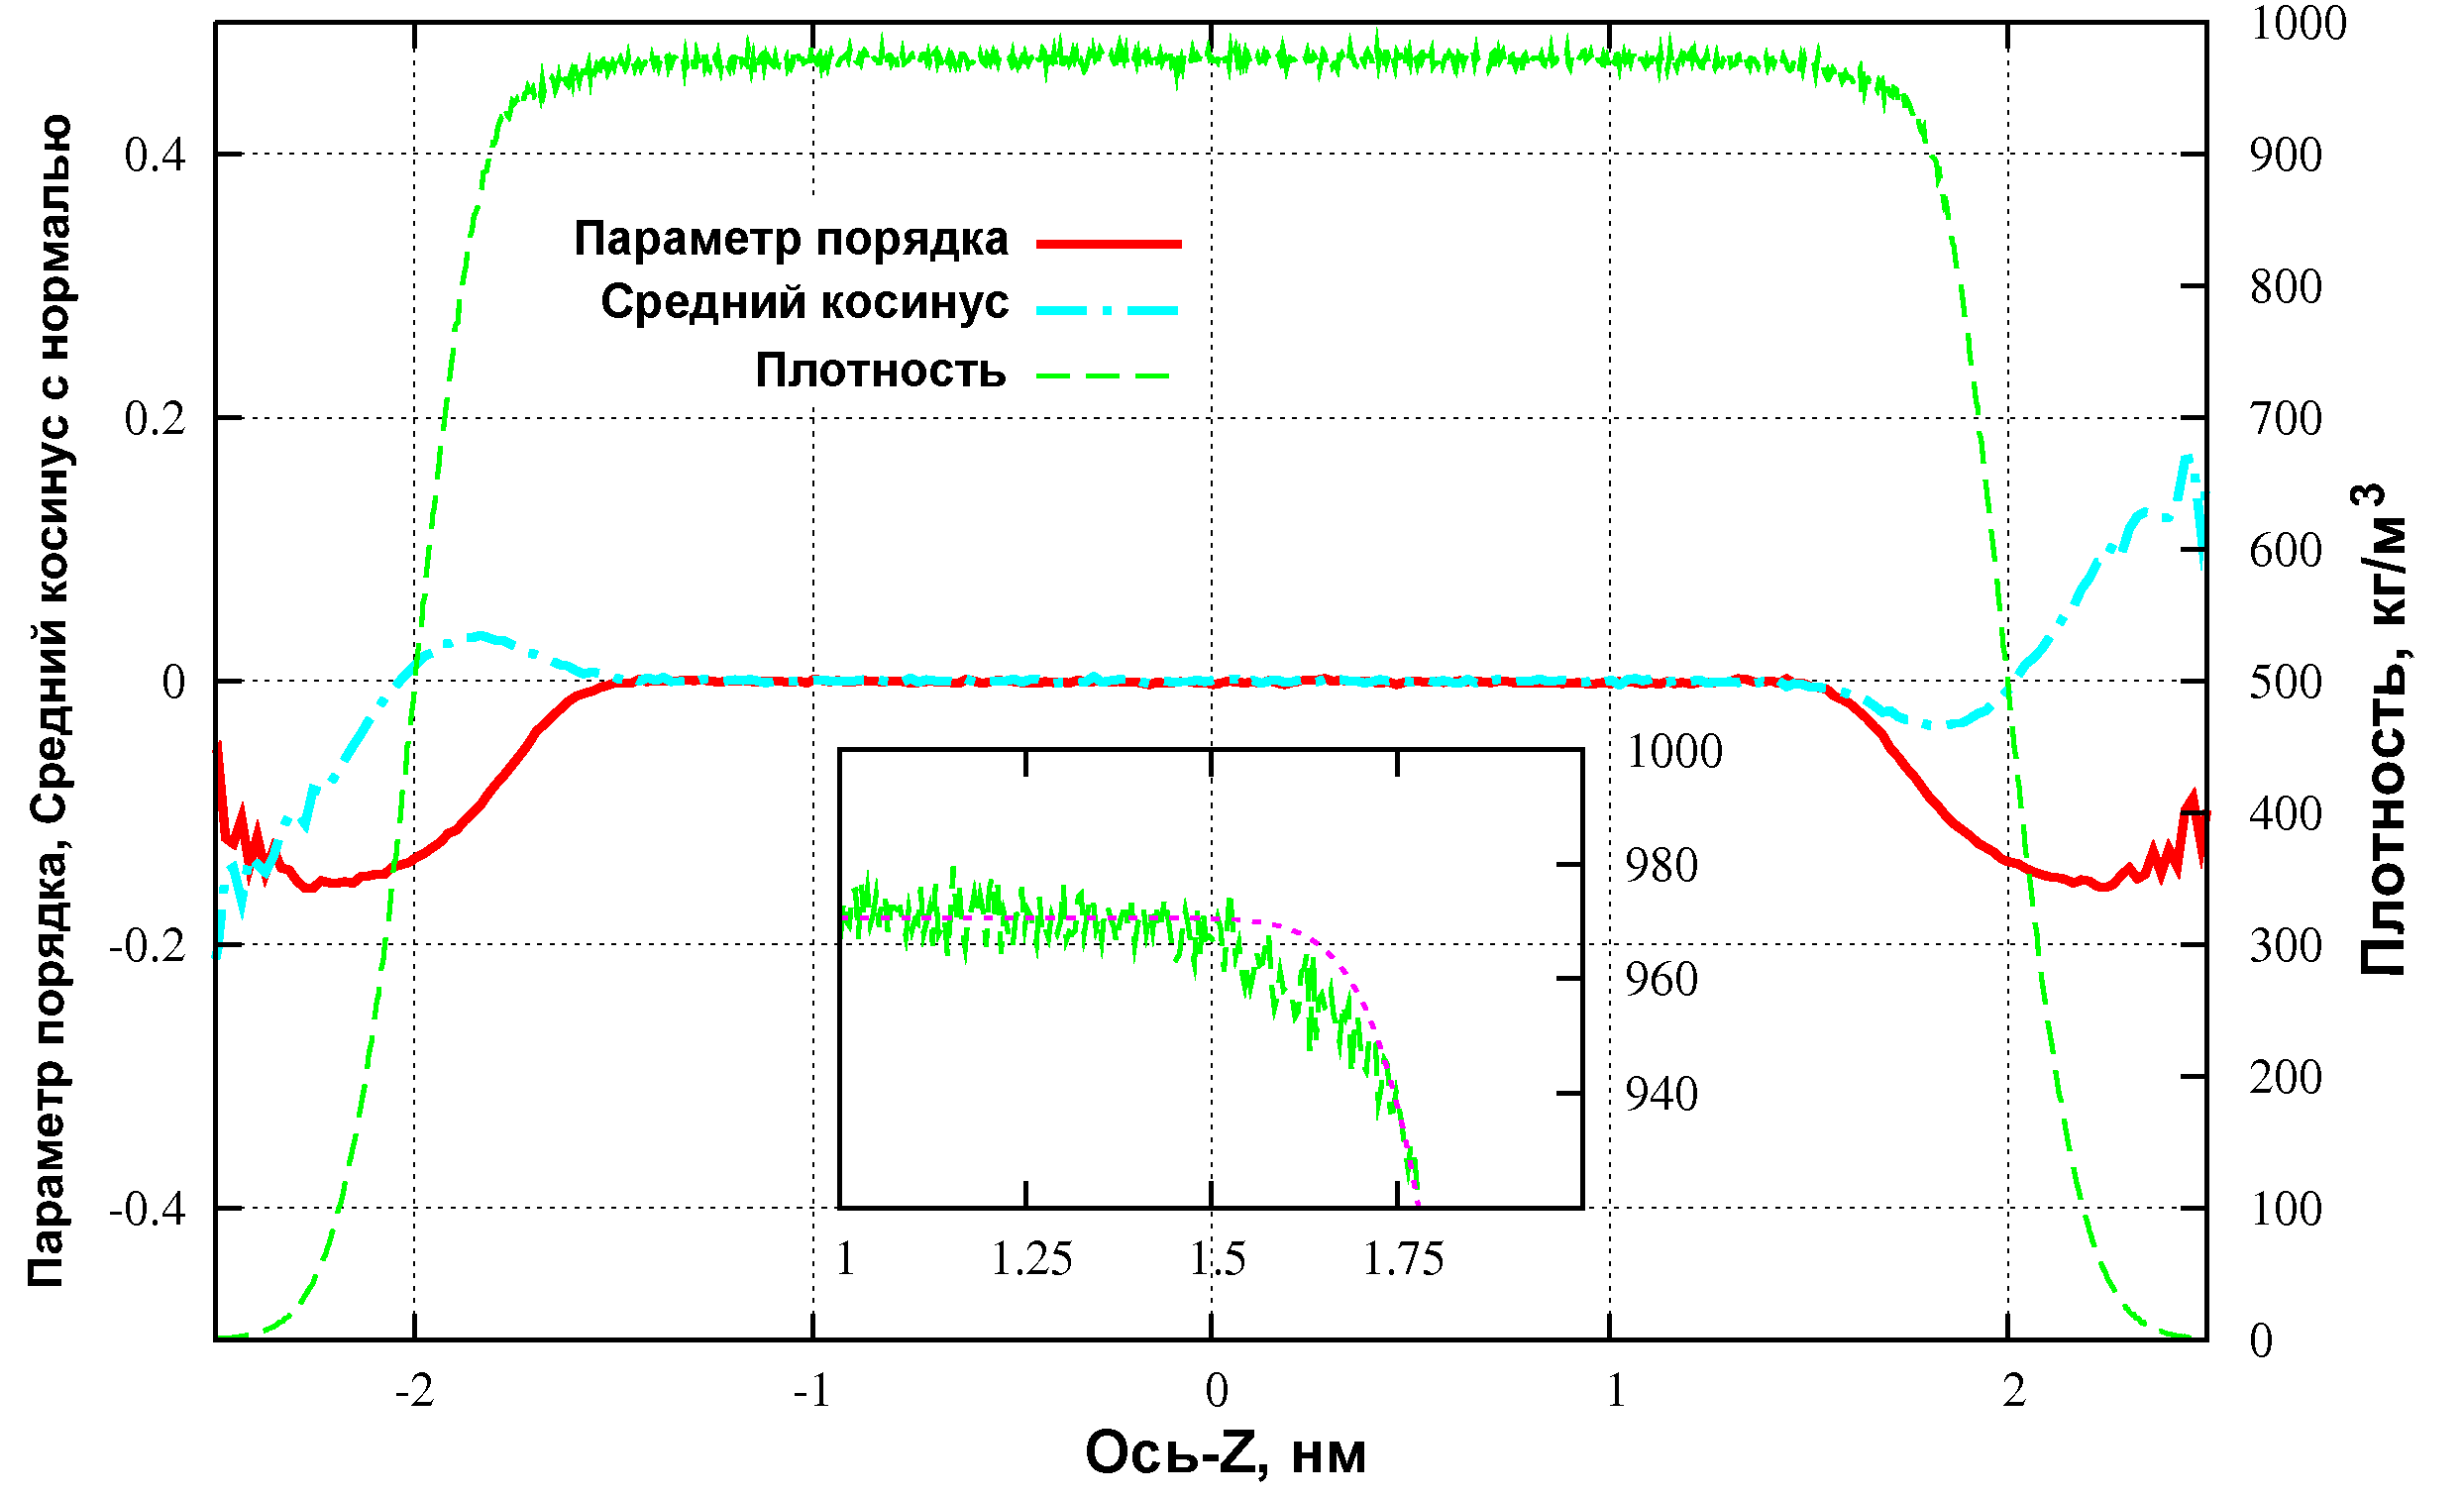
\includegraphics[width=16cm,height=10cm]{orddens}
\caption{\label{orddens} Профиль плотности водного слоя (пунктирная линия) и средние ориентационные характеристики дипольного момента молекул воды: средний косинус угла с нормалью (пунктирно-точечная линия),  параметр порядка $P_2(\cos(\theta))$ (сплошная линия). }
\end{figure}

\begin{figure}
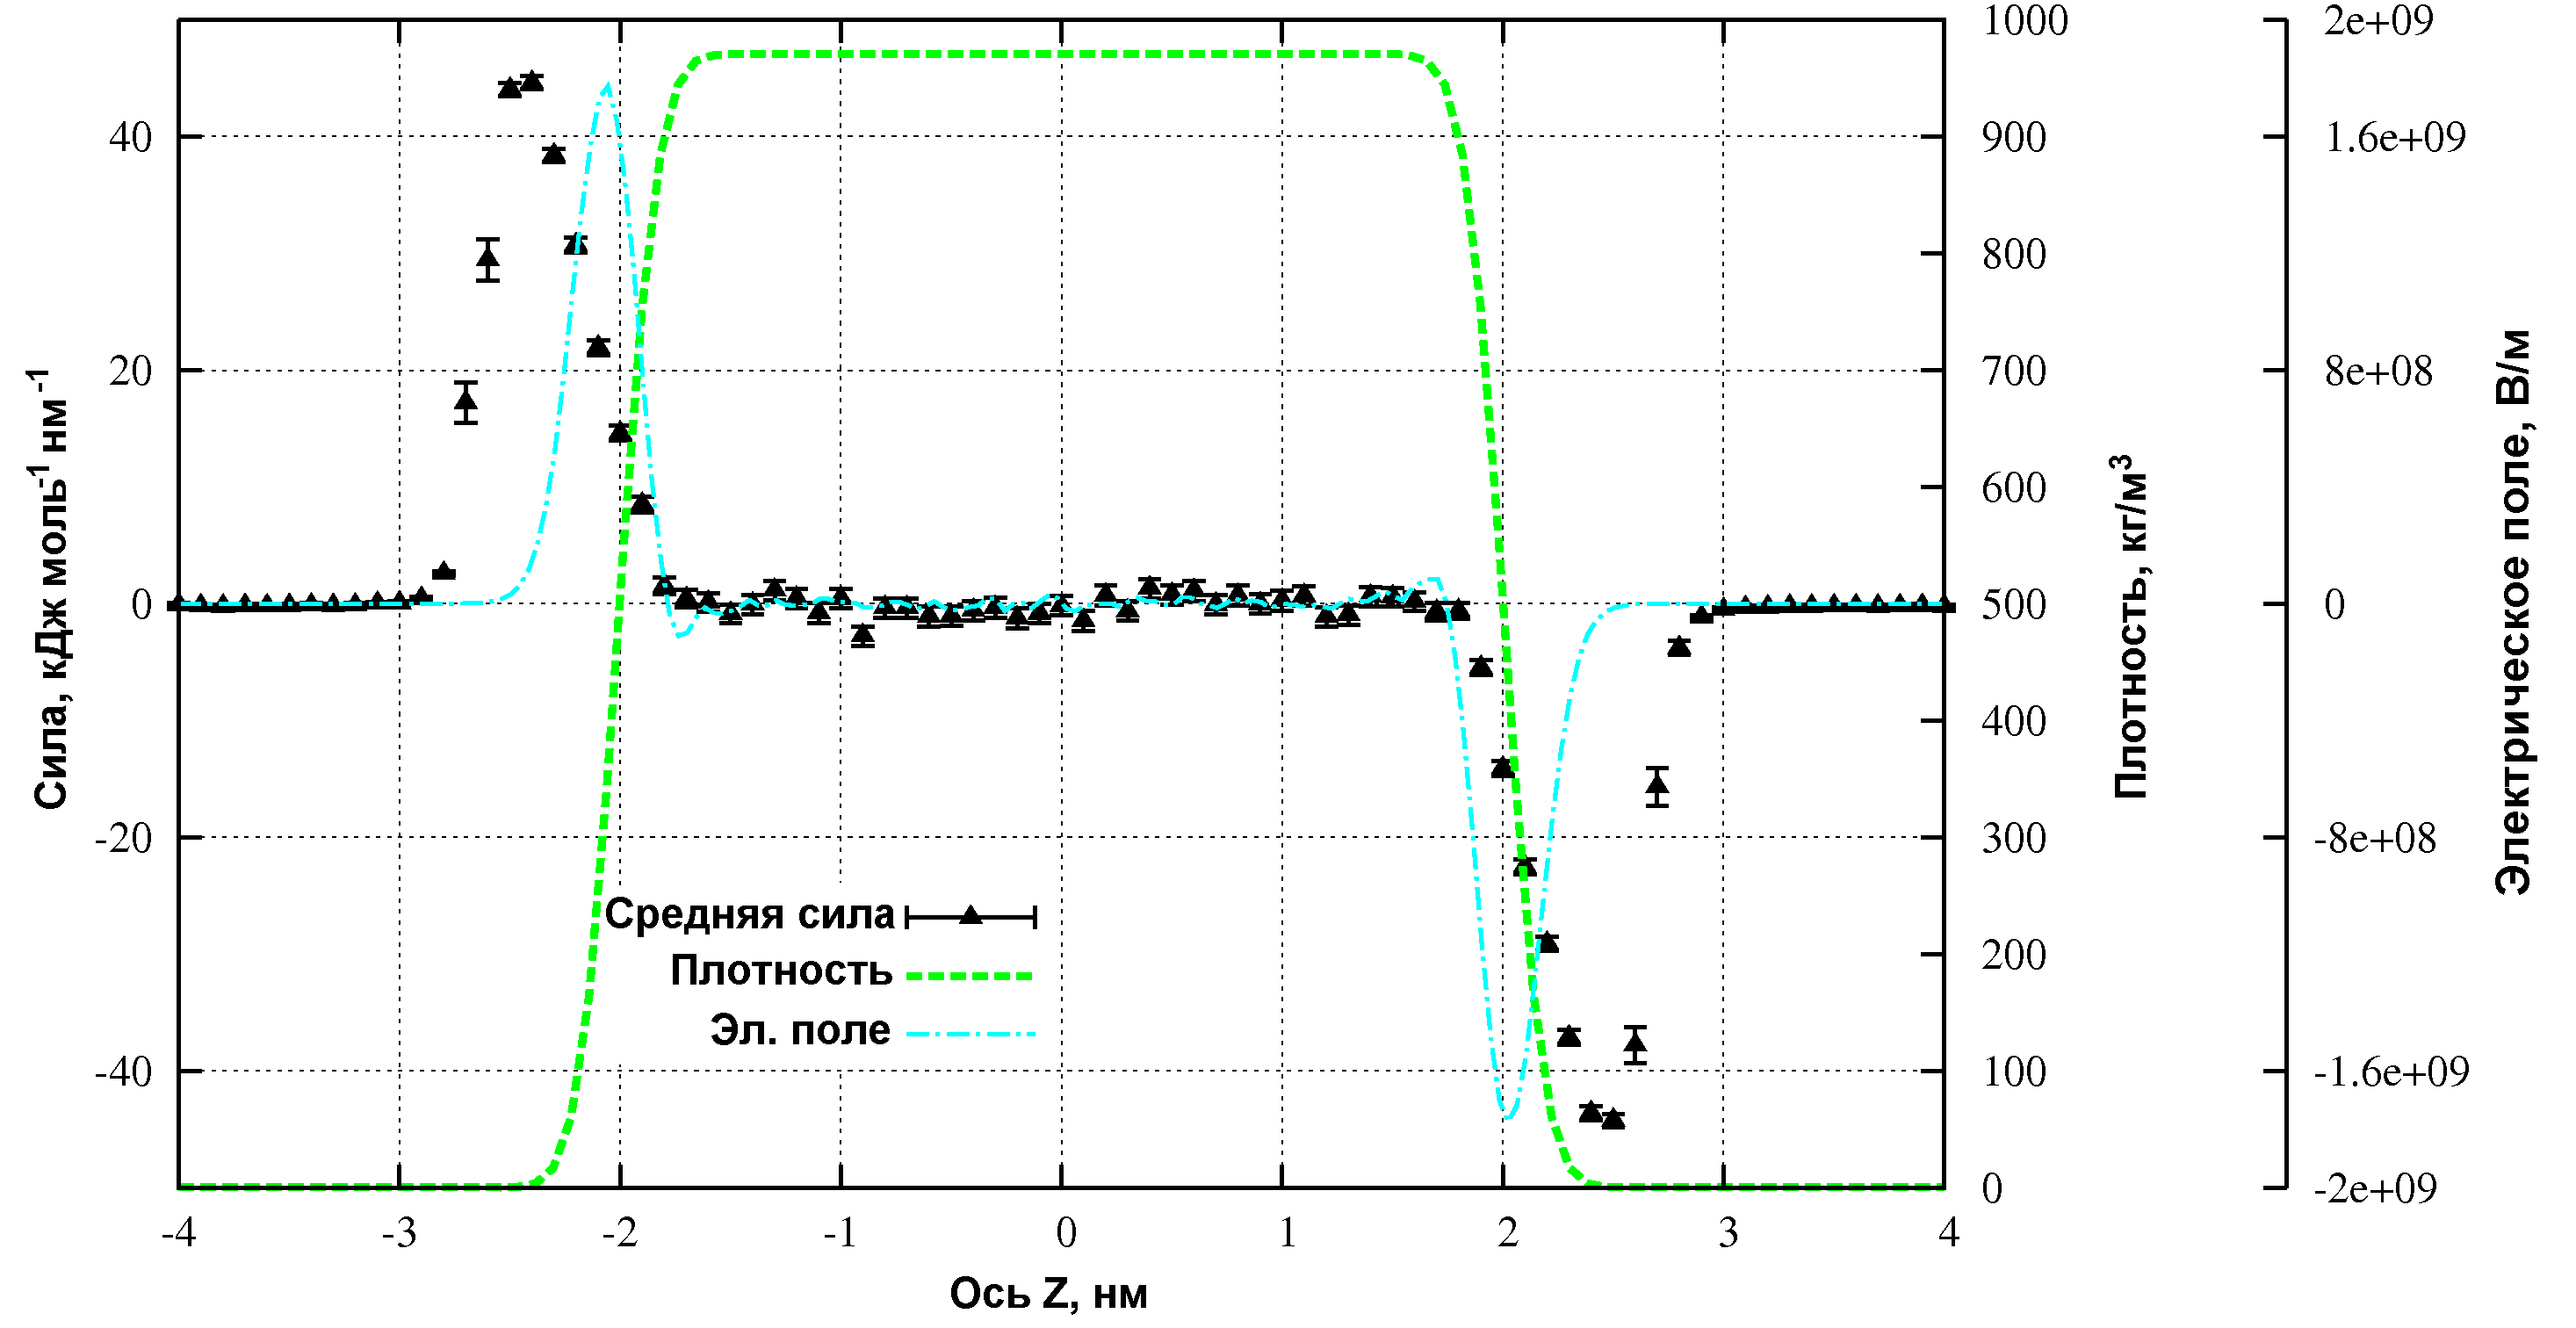
\includegraphics[width=16cm,height=8cm]{mf_d_field}
\caption{\label{mf_d_field}Профиль среднего электрического поля (пунктирно-точечная линия), профиль средней силы для одной молекулы воды (треугольники с погрешностями) как функция Z. Профиль плотности дан для сравнения (пунктирная линия).}
\end{figure}

Чтобы проанализировать ориентационное упорядочение молекул на границе мы построили
средний косинус угла с нормалью и параметр порядка $P_2(\cos{\theta})=<(3\cos{\theta}^2-1)/2>$ как функцию Z (Рис. \ref{orddens}). Видно, что дипольные моменты предпочтительно
ориентированы вдоль границы раздела. Параметр порядка $P_2(\cos{\theta})$  зануляется уже на расстоянии 0.5 нм за поверхностью Гиббса. Также небольшая ориентация диполей по нормали приводит к образованию заряженного бислоя на поверхности и соответствующего среднего электрического поля (Рис. \ref{mf_d_field}), которое достигает значений $1.7*10^{9}$ В/м в узкой области 0.7 нм около поверхности Гиббса.
Поверхностное натяжение было рассчитано на осове диагональных компонент тензора давлений по формуле $\gamma_0=\frac{L_z}{2}(P_{zz}-0.5(P_{xx}+P_{yy}))$. Получена величина $\gamma_0=51.2\pm0.8$ мН/м. Если добавить к этой величине аналитическую поправку возникающую из-за обрезки потенциала Леннард-Джонса, то получится значение 
$\gamma=55.4$ мН/м, это значение занижено по сравнению с экспериментальным (71.6 мН/м при 300K \cite{chem_handbook} ), но находится в хорошем согласии со значениями для модели SPC \cite{smith_surften}. 
 Также на примере молекулы воды была опробована техника расчёта профилей средней силы, на Рис. \ref{mf_d_field} приведён такой профиль. Энергия гидратации молекулы воды, рассчитанная из такого профиля, составляет $-25.5\pm0.7$ кДж/моль.


\subsection{\label{sec:fep_res}Профили свободной энергии}
Основной результат данного исследования -- это набор высокоточных профилей средней силы и свободной энергии для аналогов боковых цепей аминокислот на границе вода/пар. 
Типичные профили средней силы, свободной энергии и концентрации исследуемых молекул представлены на Рис. \ref{4pmf}. Симметричный вид профилей и малые значения статистических погрешностей свидетельствуют о достаточности проведённой выборки. Форма профилей средней силы похожа для всех молекул.

Рассмотрим более детально процесс сольватации с точки зрения полученных профилей.
При расстоянии более 1 нм от поверхности (здесь и далее под положением поверхности понимается положение поверхности Гиббса) нет заметного взаимодействия между молекулой и водным слоем. При дальнейшем приближении к водному слою появляется притягивающая сила, которая, очевидно, обусловлена дисперсионными и электростатическими взаимодействиями. Сила притяжения достигает своего максимума приблизительно на расстоянии 0.5 нм до поверхности Гиббса и далее сходит на нет около границы раздела. Эта область, в которой действует сила притяжения, единственная вносит отрицательный (способствующий гидратации) вклад в энергию гидратации. В таблице \ref{mean_forces} приведены параметры профилей средней силы для всех изученных молекул. Видно, что для молекул содержащих полярные группы (например, THR', ASN', GLN') максимальные значения силы притяжения намного выше, чем для чисто гидрофобных молекул. Приблизительно в районе поверхности Гиббса средняя сила обращается в ноль, что соответствует адсорбционному минимуму на графиках свободной энергии (см. Рис. \ref{4pmf}). Визуальное рассмотрение (Рис. \ref{butane_snapshots}) показывает, что максимум силы притяжения всё ещё соответствует достаточному удалению молекулы от молекул воды, хотя уже заметно некоторое возмущение водного слоя. Когда молекула продвигается далее внутрь водного слоя, возникает выталкивающая сила, которая препятствует дальнейшему погружению молекулы в воду. Причина этой силы, очевидно, может быть приписана проявлению гидрофобного эффекта: молекула вещества нарушает сеть водородных связей молекул воды, что приводит к потере энтропии молекул воды из-за сниженной подвижности последних в округе сольватируемой молекулы. Нужно отметить, что эта сила выталкивания присутствует для  всех веществ (см. Таблицу \ref{mean_forces}), точнее во всех случаях сила выталкивания оказывается сильнее силы притяжения в области сразу за поверхностью Гиббса.
Сила выталкивания пропадает при погружении молекулы на глубину 0.5-0.7 нм в зависимости от размера молекулы. После этого начинается область по своим характеристикам, неотличимая от объёма, где средняя сила взаимодействия равна нулю.
Для некоторых молекул (PHE' ,ILE' ,VAL') есть подозрение, что после области выталкивания существует опять небольшая область притяжения длиной 0.2-0.3 нм, но статистическая достоверность этого утверждения не велика.  Однако присутствие такой области приведёт к возникновению ещё одного максимума на графике свободной энергии, который иногда называют барьером десольватации, который кинетически затрудняет выход растворённого вещества из растворителя и обратно. Тот факт, что средняя сила обращается в ноль уже на расстоянии 0.5-0,7 нм за поверхностью раздела, говорит о том, что на этом расстоянии уже практически отсутствуют поверхностные эффекты влияющие на сольватацию, то есть приблизительно слой толщиной в две молекулы воды экранирует поверхность от молекулы.
\begin{table}[p]

	\begin{tabular}{lcc}
	 & $F^{max}_{at}$,кДж моль$^{-1}$нм$^{-1}$ & $F^{max}_{ex}$,кДж моль$^{-1}$нм$^{-1}$\\
	\hline
ALA'  &  5.0  &  25.8 \\
VAL'  & 10.8  &  33.1\\
LEU'  & 13.0  &  36.2\\
ILE'  & 13.1  &  34.9\\
CYS'  & 19.3  &  21.7\\
MET'  & 25.3  &  28.5\\
SER'  & 41.7  &  12.3\\
THR'  & 44.9  &  18.4\\
TYR'  & 51.3  &  27.2\\
PHE'  & 29.2  &  26.5\\
TRP'  & 51.2  &  26.5\\
ASN'  & 57.6  &  13.0\\
GLN'  & 59.9  &  20.2
\end{tabular}

	\caption{Максимальные значения средней силы притяжения и отталкивания, действующей на изучаемые молекулы по мере из прохождения через водный слой.}
	\label{mean_forces}
	\vspace{3 in}
\end{table}


\begin{figure}
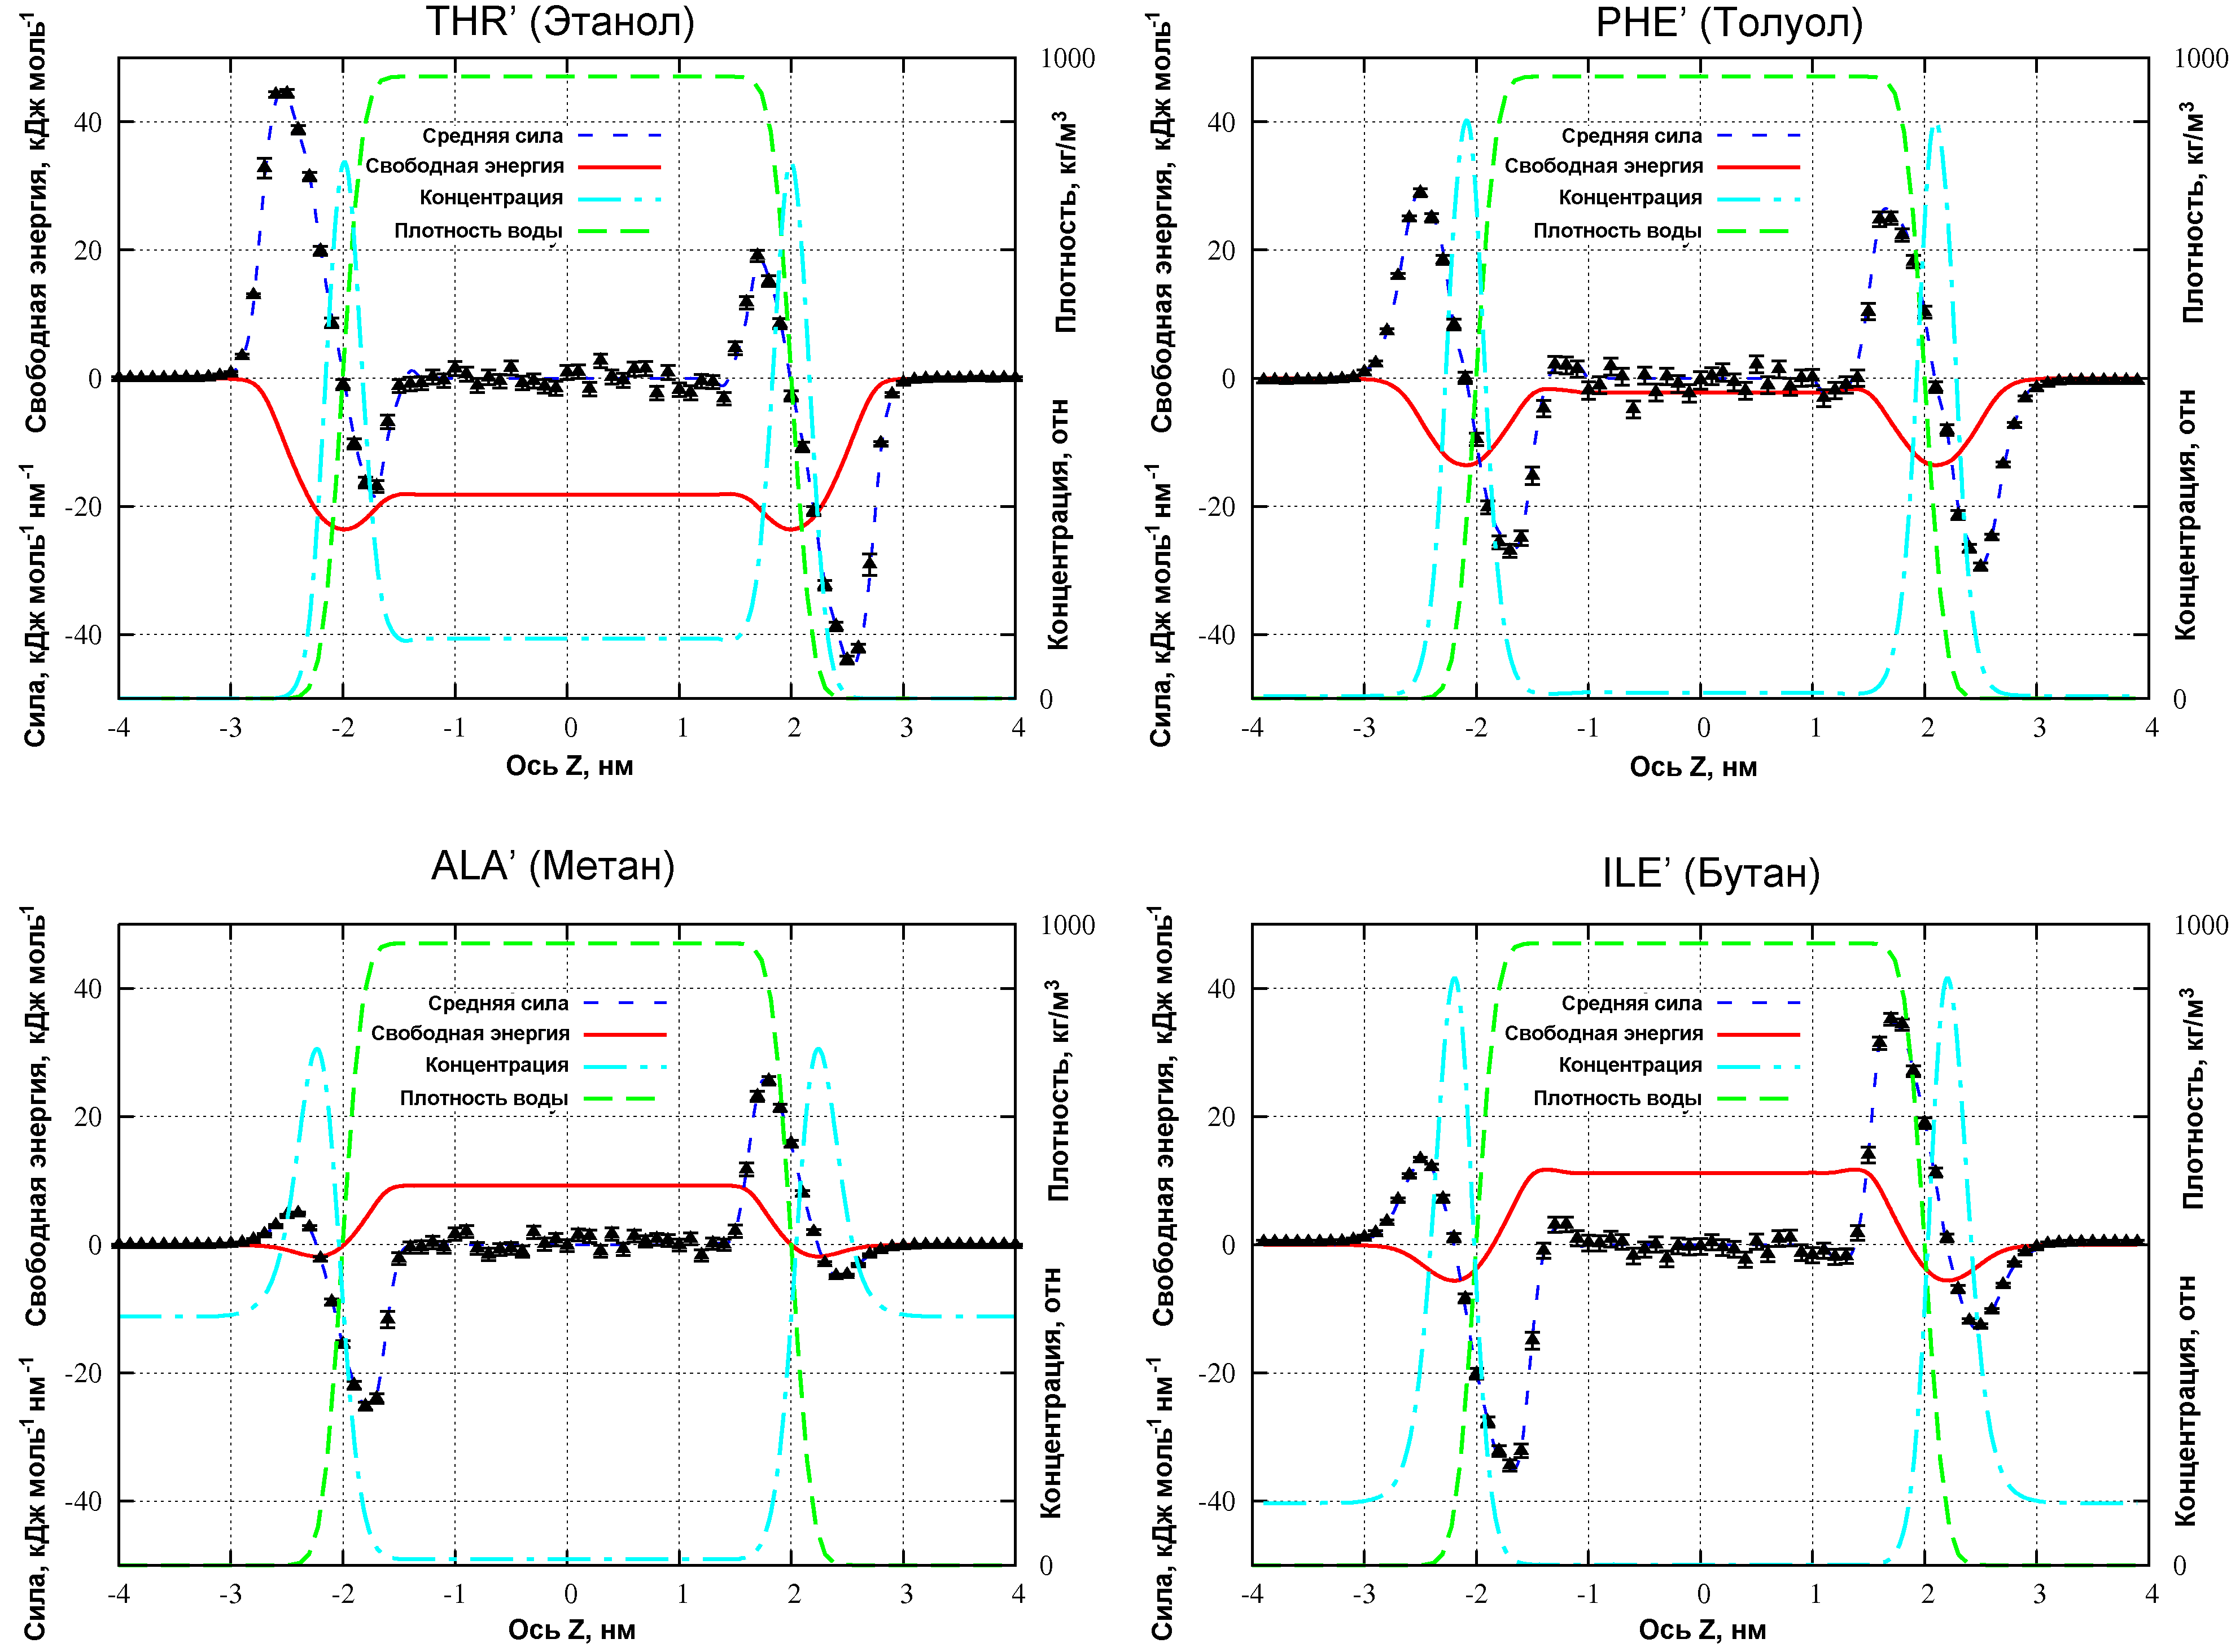
\includegraphics[width=17cm,height=13cm]{4pmf}
\caption{\label{4pmf} Профили свободной энергии для нескольких изученных молекул. Пунктирные линии и точки с отмеченными погрешностями -- профиль средней силы и его сплайн аппроксимация (погрешности отмечены как $\pm$ одно стандартное отклонение). Сплошная линия - профиль свободной энергии, пунктирно-точечная линия - относительный профиль концентрации, рассчитанный по профилю свободной энергии. Для сравнения пунктирной линией отмечен профиль плотности водного слоя.}
\end{figure}

\begin{figure}
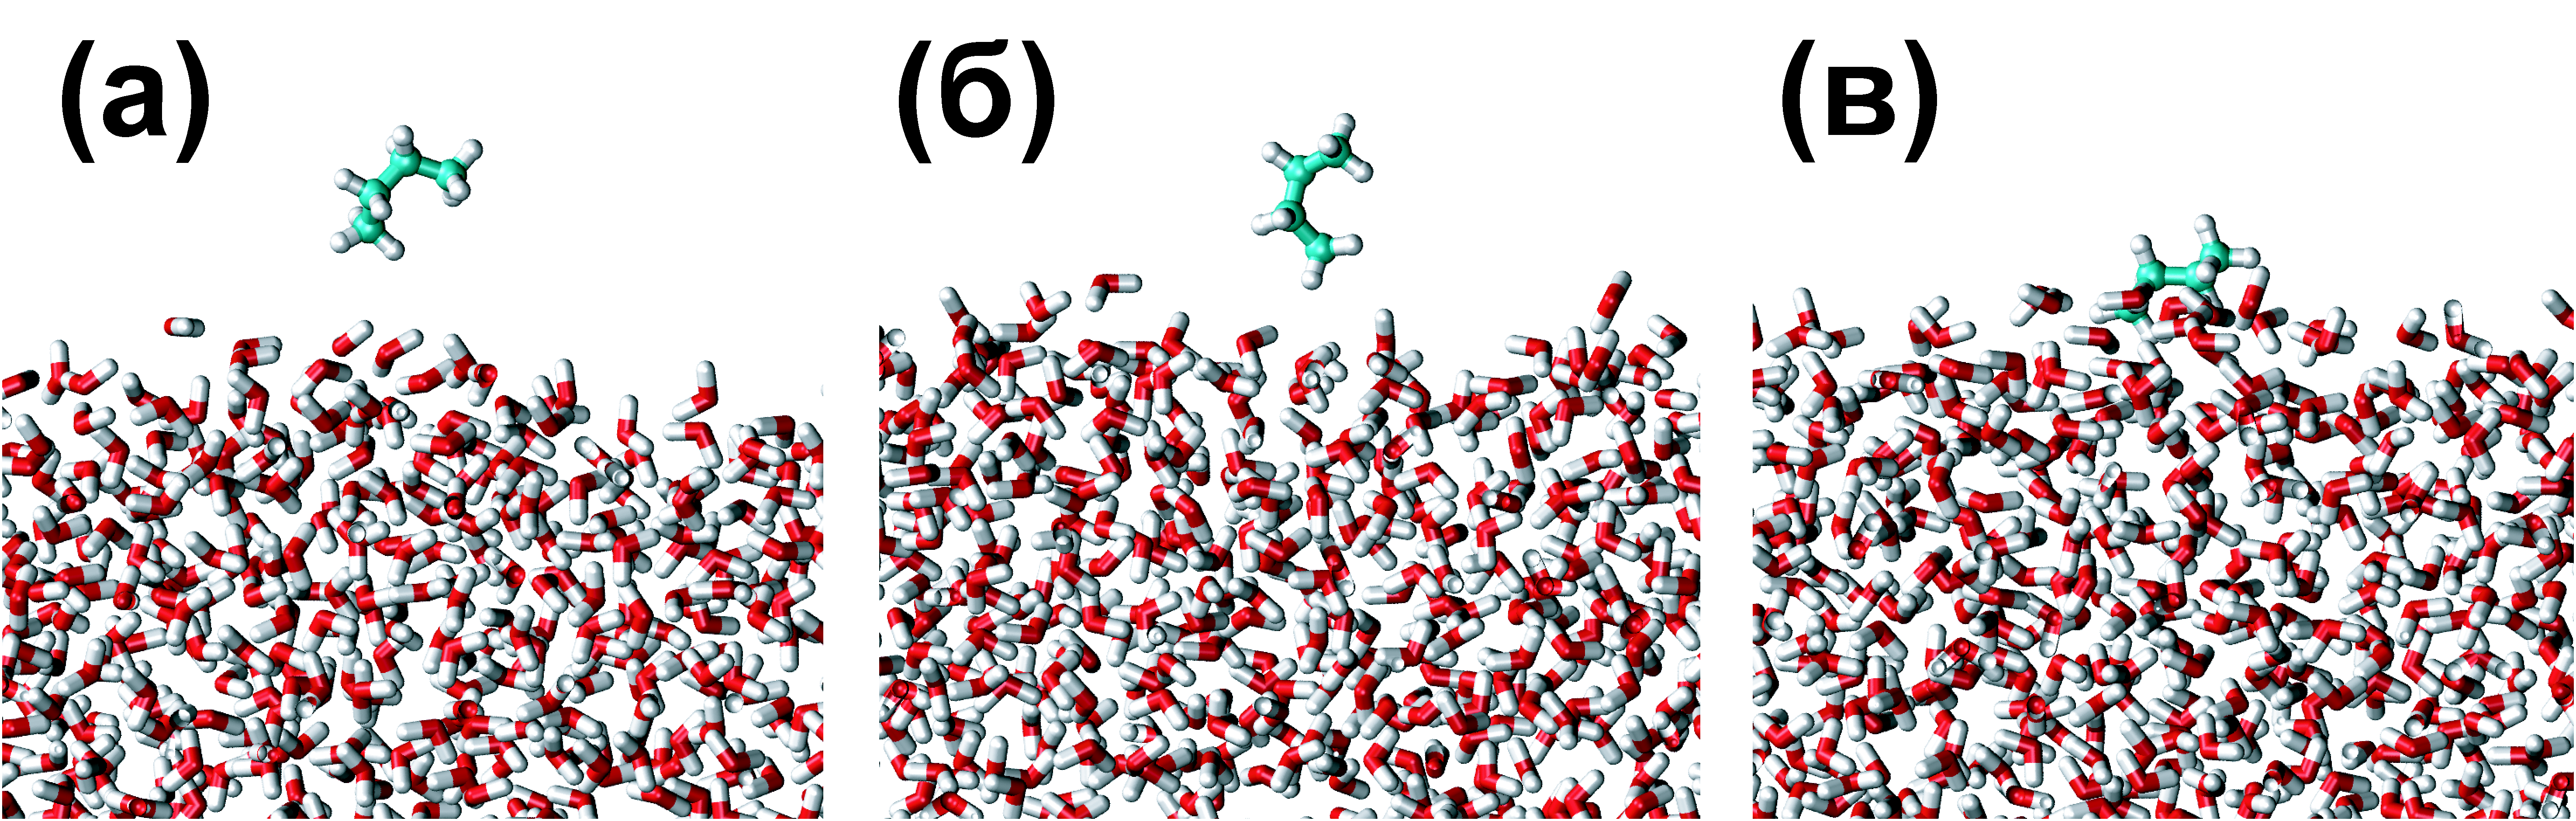
\includegraphics[width=17cm,height=5.5cm]{butane_snapshots}
\caption{\label{butane_snapshots} Мгновенные изображения молекулы бутана во время расчётов на различных расстояниях от границы раздела. Положения соответствующие: (а) максимальной силе притяжения, (b) адсорбционному минимуму, (с) максимальной выталкивающей силе.}
\end{figure}

\subsection{\label{sec:comp_exp}Количественные результаты}
В данном разделе обсудим численные результаты расчётов энергий гидратации и адсорбции. Энергии гидратации были определены двумя способами: как значения профилей свободной энергии в середине слоя, и с помощью метода Беннетта (BAR) из расчётов в объёме. Последние результаты, несомненно, более надёжные, поскольку мало зависят от конечномерных эффектов, дают адекватную оценку статистической погрешности, а также сам метод является методологически хорошо изученным. Поэтому результаты этого метода будут использоваться для критической оценки результатов расчёта профилей свободной энергии.
Результаты обоих методов, а также экспериментальные значения приведены в таблице \ref{hydr_fe}.

\begin{table}[p]
\caption{Энергии гидратации боковых цепей аминокислот, полученные различными методами (методом Беннетта и по профилям свободной энергии), и экспериментальные результаты. Для метода Беннетта статистическая погрешность приведена как одно стандартное отклонение.}
	\label{hydr_fe}

\begin{threeparttable}	
	\begin{tabular}{lccc}
	 & $G^{hydr}_{BAR}$,кДж моль$^{-1}$& $G^{hydr}_{PMF}$,кДж моль$^{-1}$& $G^{hydr}_{exp}$,кДж моль$^{-1}$\tnote{a}\\
	\hline

ALA'  &$  9.20\pm0.04 $& $9.3\pm0.6\tnote{b} $&   8.12  \\
VAL'  &$ 10.1 \pm0.1  $&$ 10.9\pm0.7$ &   8.33  \\
LEU'  &$ 10.57\pm0.08 $&$ 11.3\pm0.8$ &   9.54  \\
ILE'  &$ 10.5\pm 0.3  $&$ 11.7\pm0.7$ &   9.00   \\
CYS'  &$ -2.24\pm0.06 $&$ -1.2\pm0.6$&  -5.19  \\
MET'  &$ -1.74\pm0.18 $&$ -0.5\pm0.7$&  -6.19   \\
SER'  &$-19.2\pm 0.1  $&$ -18.9\pm0.6$& -21.17  \\
THR'  &$-18.65\pm0.13 $&$ -18.1\pm0.7$& -20.42   \\
TYR'  &$-22.33\pm0.18 $&$ -20.5\pm0.9$& -25.56   \\
PHE'  &$ -3.26\pm0.11 $&$ -1.6\pm0.8$&  -3.18  \\
TRP'  &$-18.7\pm 0.3  $&$ -15.9\pm0.9$& -24.60   \\
ASN'  &$-35.69\pm0.10 $&$ -33.6\pm0.9$& -40.50   \\
GLN'  &$-36.45\pm0.16 $&$-32.7\pm0.9$& -39.26  \\
\end{tabular}
\begin{tablenotes}	
	\item[a]{Экспериментальные значения из работы \cite{wolfenden_1988}.}
	\item[b]{Статистические погрешности не включают какие-либо систематические погрешности или погрешности силового поля и методологии.}
\end{tablenotes}
\end{threeparttable}

		
	\vspace{3 in}
\end{table}
Результаты полученные методом BAR находятся в очень хорошем согласии с другими работами \cite{shirts_waterff}. Обсуждения совпадения и отличий данных моделирования и эксперимента может быть найдено в работе \cite{shirts_waterff}: основной вывод состоит в том, что корреляция результатов очень хорошая (в нашем случае коэффициент корреляции равен 0.997), однако абсолютные значения оказываются на 2-4 кДж/моль выше, чем экспериментальные.


Из таблицы \ref{hydr_fe} видно, что статистические погрешности значений рассчитанных из профилей свободной энергии несколько выше (около 1 кДж/моль). Видно, что хотя значения энергий для отдельных веществ (5 из 13) в обоих методах согласуются в пределах статистической погрешности, все значения полученные путём интегрирования профиля средней силы завышены относительно ``настоящих'' модельных значений. Несостыковки ранжируются от 0 для ALA' до 4 кДж/моля для GLN'. Причина этих расхождений, на наш взгляд, кроется в (i) невозможности интегрирования хвоста профиля из-за наличия статистической ошибки в значениях силы, (ii) конечном размере водного слоя и (iii) обрезки потенциала Леннард-Джонса при невозможности применения аналитической поправки (что возможно при расчётах в объёме метдом BAR). Приблизительная оценка теряемой энергии при обрезке потенциала Леннард-Джонса в нашем случае будет варьироваться от 0.4 кДж/моль для ALA' до 3 кДж/моль для TRP'. Применение этих поправок уже сильно бы улучшило совпадения результатов. Однако пока алгоритмы учёта таких поправок для негомогенных систем не развиты.

Мы измерили энергии адсорбции двумя способами: используя подход Гиббса и путём измерения значения профиля энергии в минимуме. В подходе Гиббса сначала рассчитывался относительный профиль концентрации, предполагая концентрацию в газовой фазе равной 1 нм$^{-3}$. Затем рассчитывался избыток Гиббса по формуле \ref{excess} и энергия адсорбции оценивалась по формуле \ref{ads_fe_eq}, предполагая толщину границы раздела равной 1 нм, поскольку это обычно была толщина, на которой варьировался профиль свободной энергии.
Оба набора полученных энергий (см. таблицу \ref{ads_fe}) находятся в отличной корреляции (R=0.9996), хотя заметны некоторые отклонения для веществ с низкой поверхностной активностью, для последних, очевидно, метод имеет значение. Хотя значение энергии в минимуме оказалось хорошей оценкой энергии адсорбции, предположительно метод Гиббса является более универсальным и термодинамически корректным. 

% \begin{equation}
% \Gamma^i=\int_{-\infty}^{z_0}(c^i(z)-c^i_1)dz+\int_{z_0}^{\infty}(c^i(z)-c^i_2)dz
% \label{excess}
% \end{equation}

% \begin{equation}
% G_{ads}=-kT\ln{\frac{\Gamma^S}{c^S\tau}}
% \label{ads_fe_eq}
% \end{equation}


\begin{table}[p]
\caption{Сродство изученных молекул к поверхности, характеризуемое идеальными величинами избытка Гиббса (предполагая концентрацию молекул в фазе пара 1 нм$^{-3}$), энергиями адсорбции Гиббса и глубиной энергии адсорбционного минимума. Последняя колонка представляет энергию адсорбции Гиббса по отношению к фазе максимального сродства.}
	\label{ads_fe}	
	\begin{tabular}{lcccc}
	 & $\Gamma^{excess}$,нм$^{-2}$& $G^{ads}_{Gibbs}$,кДж моль$^{-1}$& $G^{ads}_{min}$,кДж моль$^{-1}$&$G^{ads}_{aff}$,кДж моль$^{-1}$\\
	\hline

ALA'  &$  0.544       $&   1.52 &  -1.82 &  1.52\\
VAL'  &$  2.3         $&  -2.08 &  -4.45 & -2.08\\
LEU'  &$  3.8         $&  -3.33 &  -5.64 & -3.33\\
ILE'  &$  3.7         $&  -3.27 &  -5.59 & -3.27\\
CYS'  &$ 14.0         $&  -6.61 &  -8.76 & -4.37\\
MET'  &$ 57.0         $& -10.1  & -12.35 & -8.36\\
SER'  &$ 2.1*10^3     $& -19.12 & -22.03 &  0.08\\
THR'  &$ 4.7*10^3     $& -21.1  & -23.61 & -2.45\\
TYR'  &$ 65.0*10^3    $& -27.63 & -30.05 & -5.30\\
PHE'  &$ 95.0         $& -11.37 & -13.59 & -8.11\\
TRP'  &$ 22.6*10^3    $& -25.0  & -27.47 & -6.3\\
ASN'  &$0.74*10^6     $& -33.71 & -37.03 &  1.99\\
GLN'  &$2.30*10^6     $& -36.52 & -39.15 & -0.02\\
\end{tabular}
	
	
	\vspace{3 in}
\end{table}


Значения энергии адсорбции Гиббса в таблице \ref{ads_fe} представлены относительно фазы максимального сродства (как обычно делается в экспериментальных работах). Можно сказать, что все вещества являются поверхностно активными в том плане, что в профилях свободной энергии у них есть адсорбционный минимум. Однако конченые значения энергии адсорбции всегда являются относительными поскольку зависят от определения стандартных состояний и условной толщины границы раздела.

К сожалению, в литературе встречается мало экспериментальных данных, с которыми можно было бы сравнить полученные численные данные. Бул и Бриз \cite{bull_breese} ввели шкалу энергий адсорбции для боковых цепей аминокислот, руководствуясь данными по измерению поверхностного натяжения для цвиттерионых аминокислот и применяя предположение об аддитивности вкладов различных молекулярных групп. Однако, если предположение об аддитивности достаточно хорошо себя зарекомендовало при оценках энергий сольватации, то в случае измерения энергий адсорбции справедливость такого предположения вызывает сомнения.
Коэффициент корреляции шкалы Була и Бриза с модельными результатами по адсорбции составляет 0.65.

Измерения избытка Гиббса для метанола и этанола были проведены с помощью нейтронного рассеяния \cite{eth-excess-exp,meth-excess-exp} и равны  2.5*10$^{-10}$ моль*см$^{-2}$ и (3-5)*10$^{-10}$ моль*см$^{-2}$, соответственно, при объёмной концентрации в 0.0012 моль*см$^{-3}$. Эти данные находятся в разумном согласии с результатами нашей модели равными 1.2*10$^{-10}$ моль*см$^{-2}$ и 2.6*10$^{-10}$ моль*см$^{-2}$ для этого случая. По данным работы \cite{atmgas_excess-exp} на основании измерения поверхностного натяжения энергия адсорбции метанола из газовой фазы составляет $-15.2\pm0.5$ кДж/моль, в то время как из наших расчётов следует величина -19.2. кДж/моль.


Следуя идеям статьи Охапкина и др. \cite{okhapkin_amino}, нами были построены двумерные диаграммы сродства молекул к объёмной и поверхностной фазе воды (Рис. \ref{diagr}) по двум параметрам: энергии гидратации и энергии адсорбции относительно фазы максимального сродства. Видно, что изученные молекулы покрывает достаточно большую область энергий адсорбции и гидратации. Некоторые молекулы обладают сходными характеристиками, например, (i) PHE' и MET', (ii) VAL',ILE' и LEU',  (iii) ASN' и GLN'. Однако, в общем можно заключить, что корреляции между энергиями адсорбции относительно фазы максимального сродства и гидратации в нашем случае не наблюдается, эти характеристики являются независимыми и в то же время достаточно простыми параметрами, описывающими взаимодействие растворителя с другими веществами, которые могут использоваться для улучшения и уточнения молекулярных моделей и силовых полей подобно тому, как для этого используются только энергии гидратации \cite{gromos_hydr}.

\begin{figure}
\centering
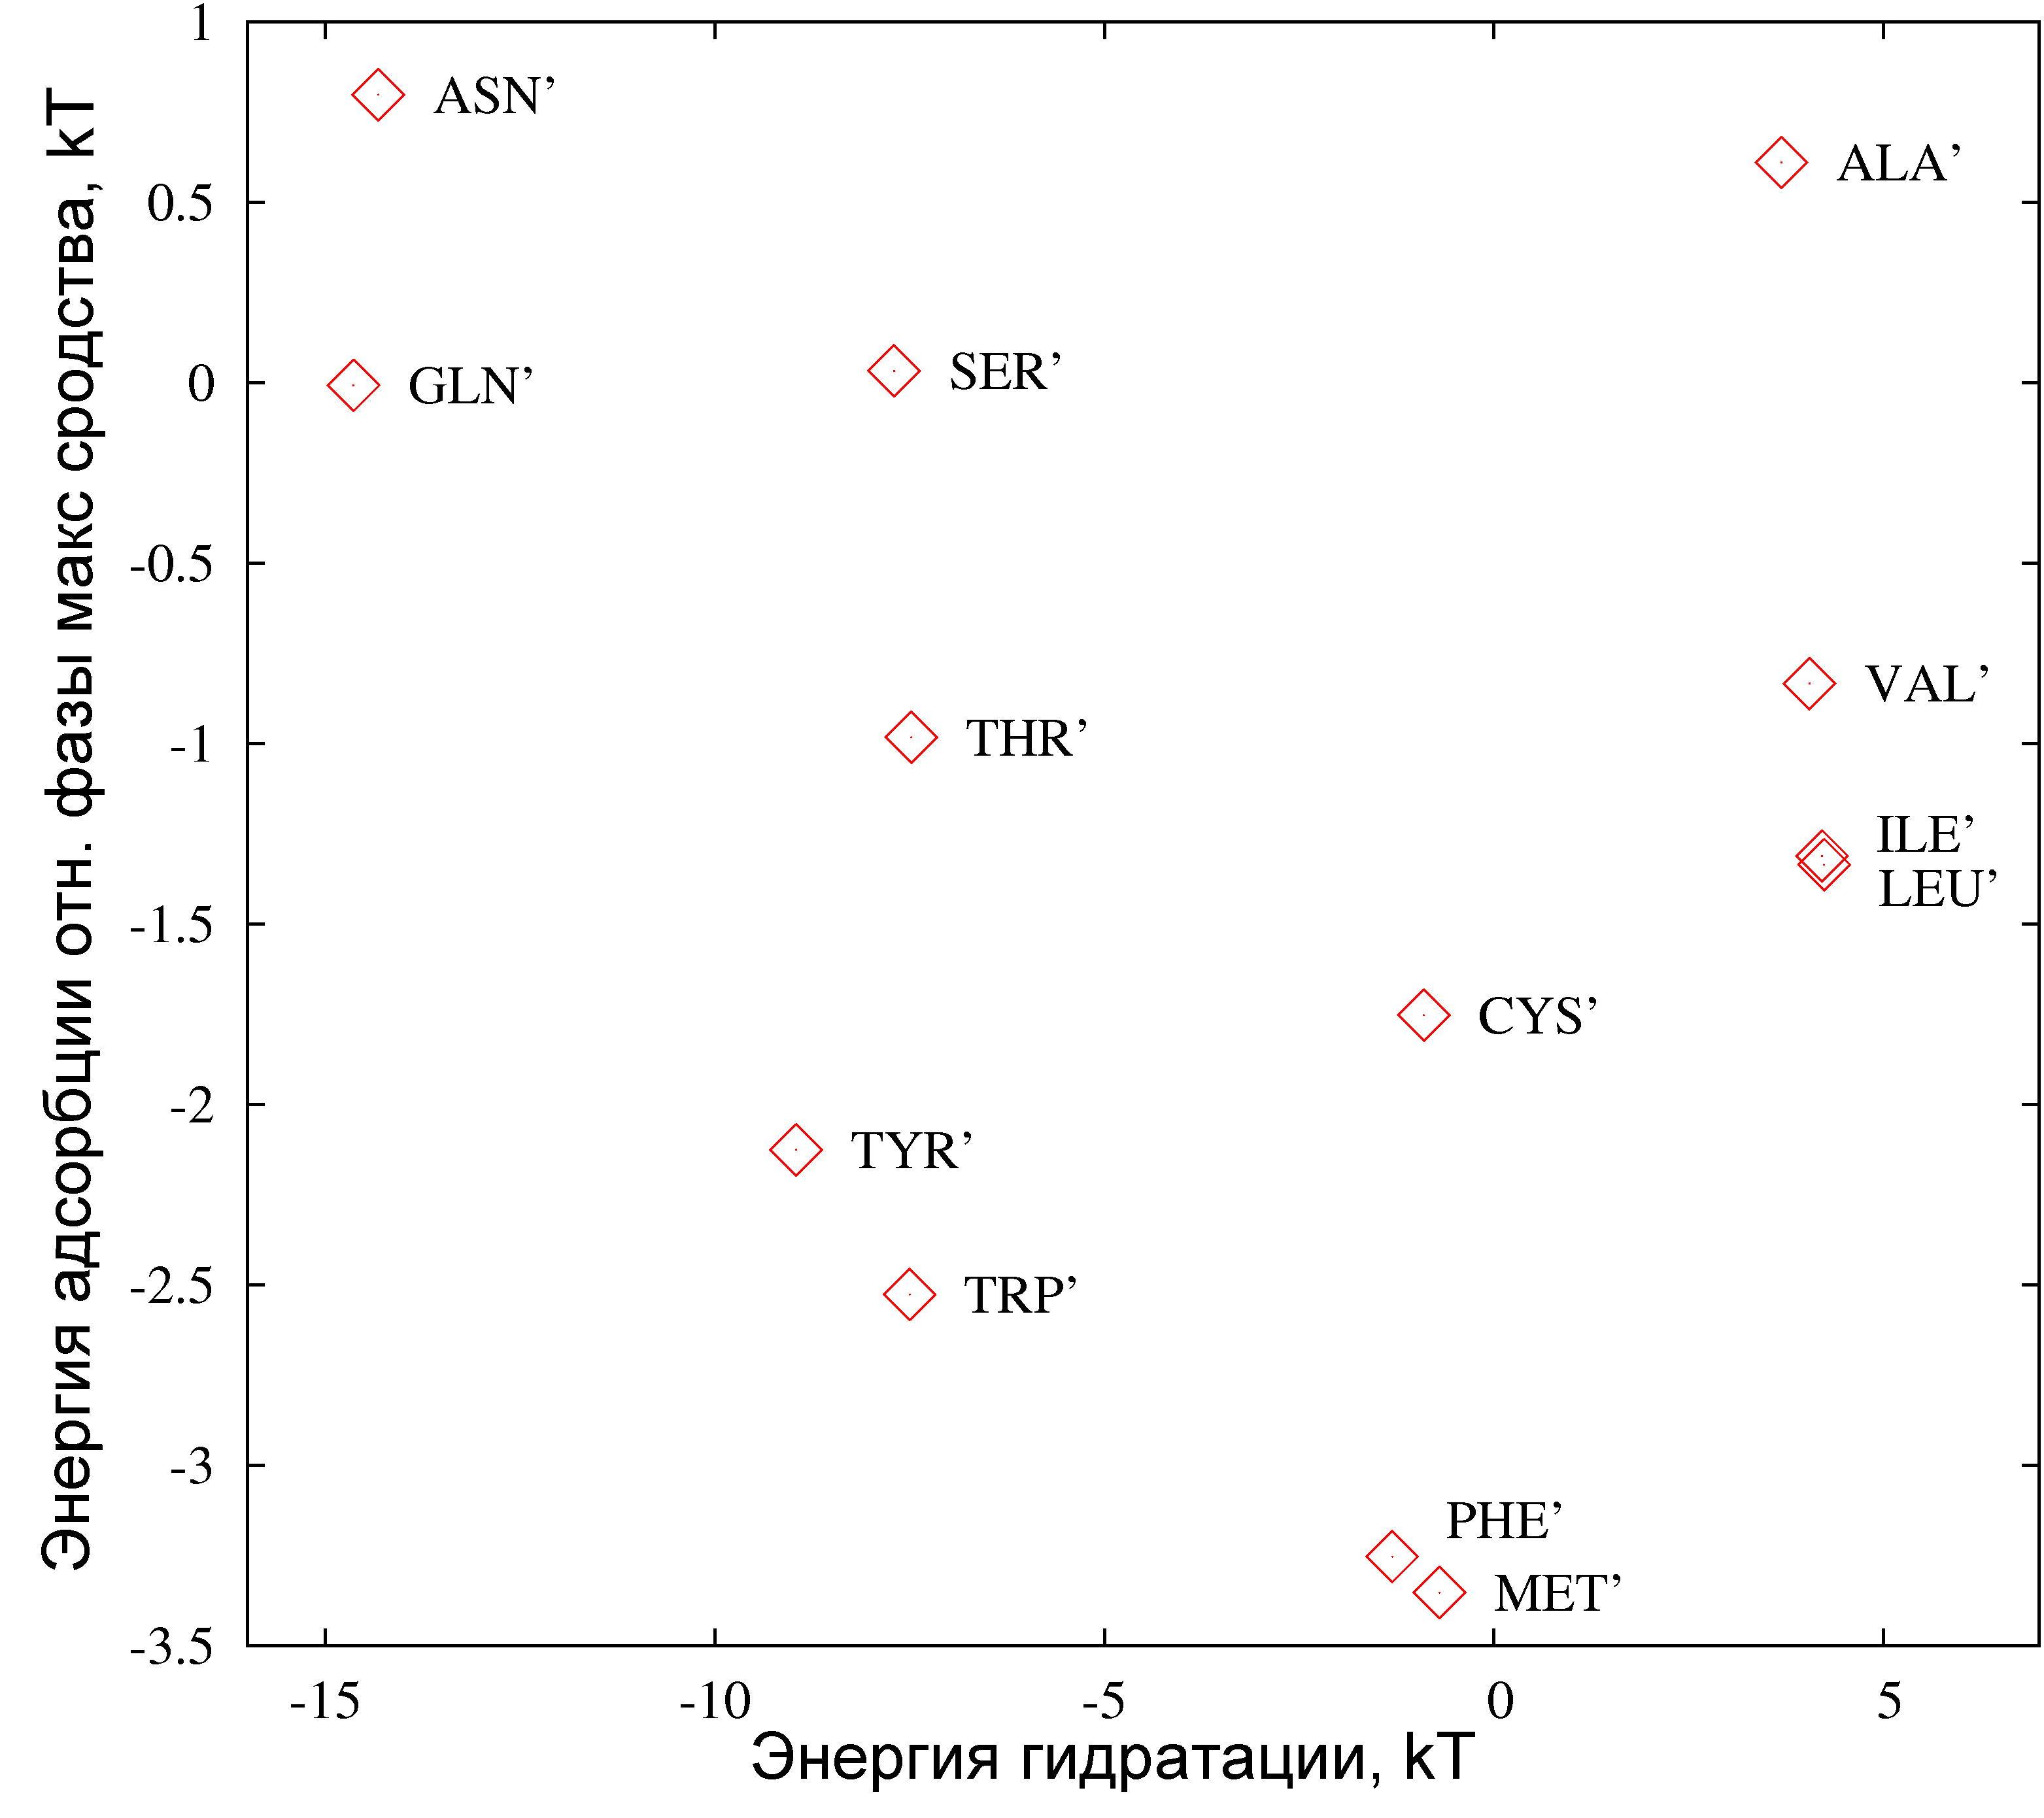
\includegraphics[width=10cm]{diagr}
\caption{\label{diagr} Двумерная классификационная диаграмма для исследованных веществ в координатах энергия гидратации - энергия адсорбции относительно фазы максимального сродства.}
\end{figure}

\begin{figure}
\centering
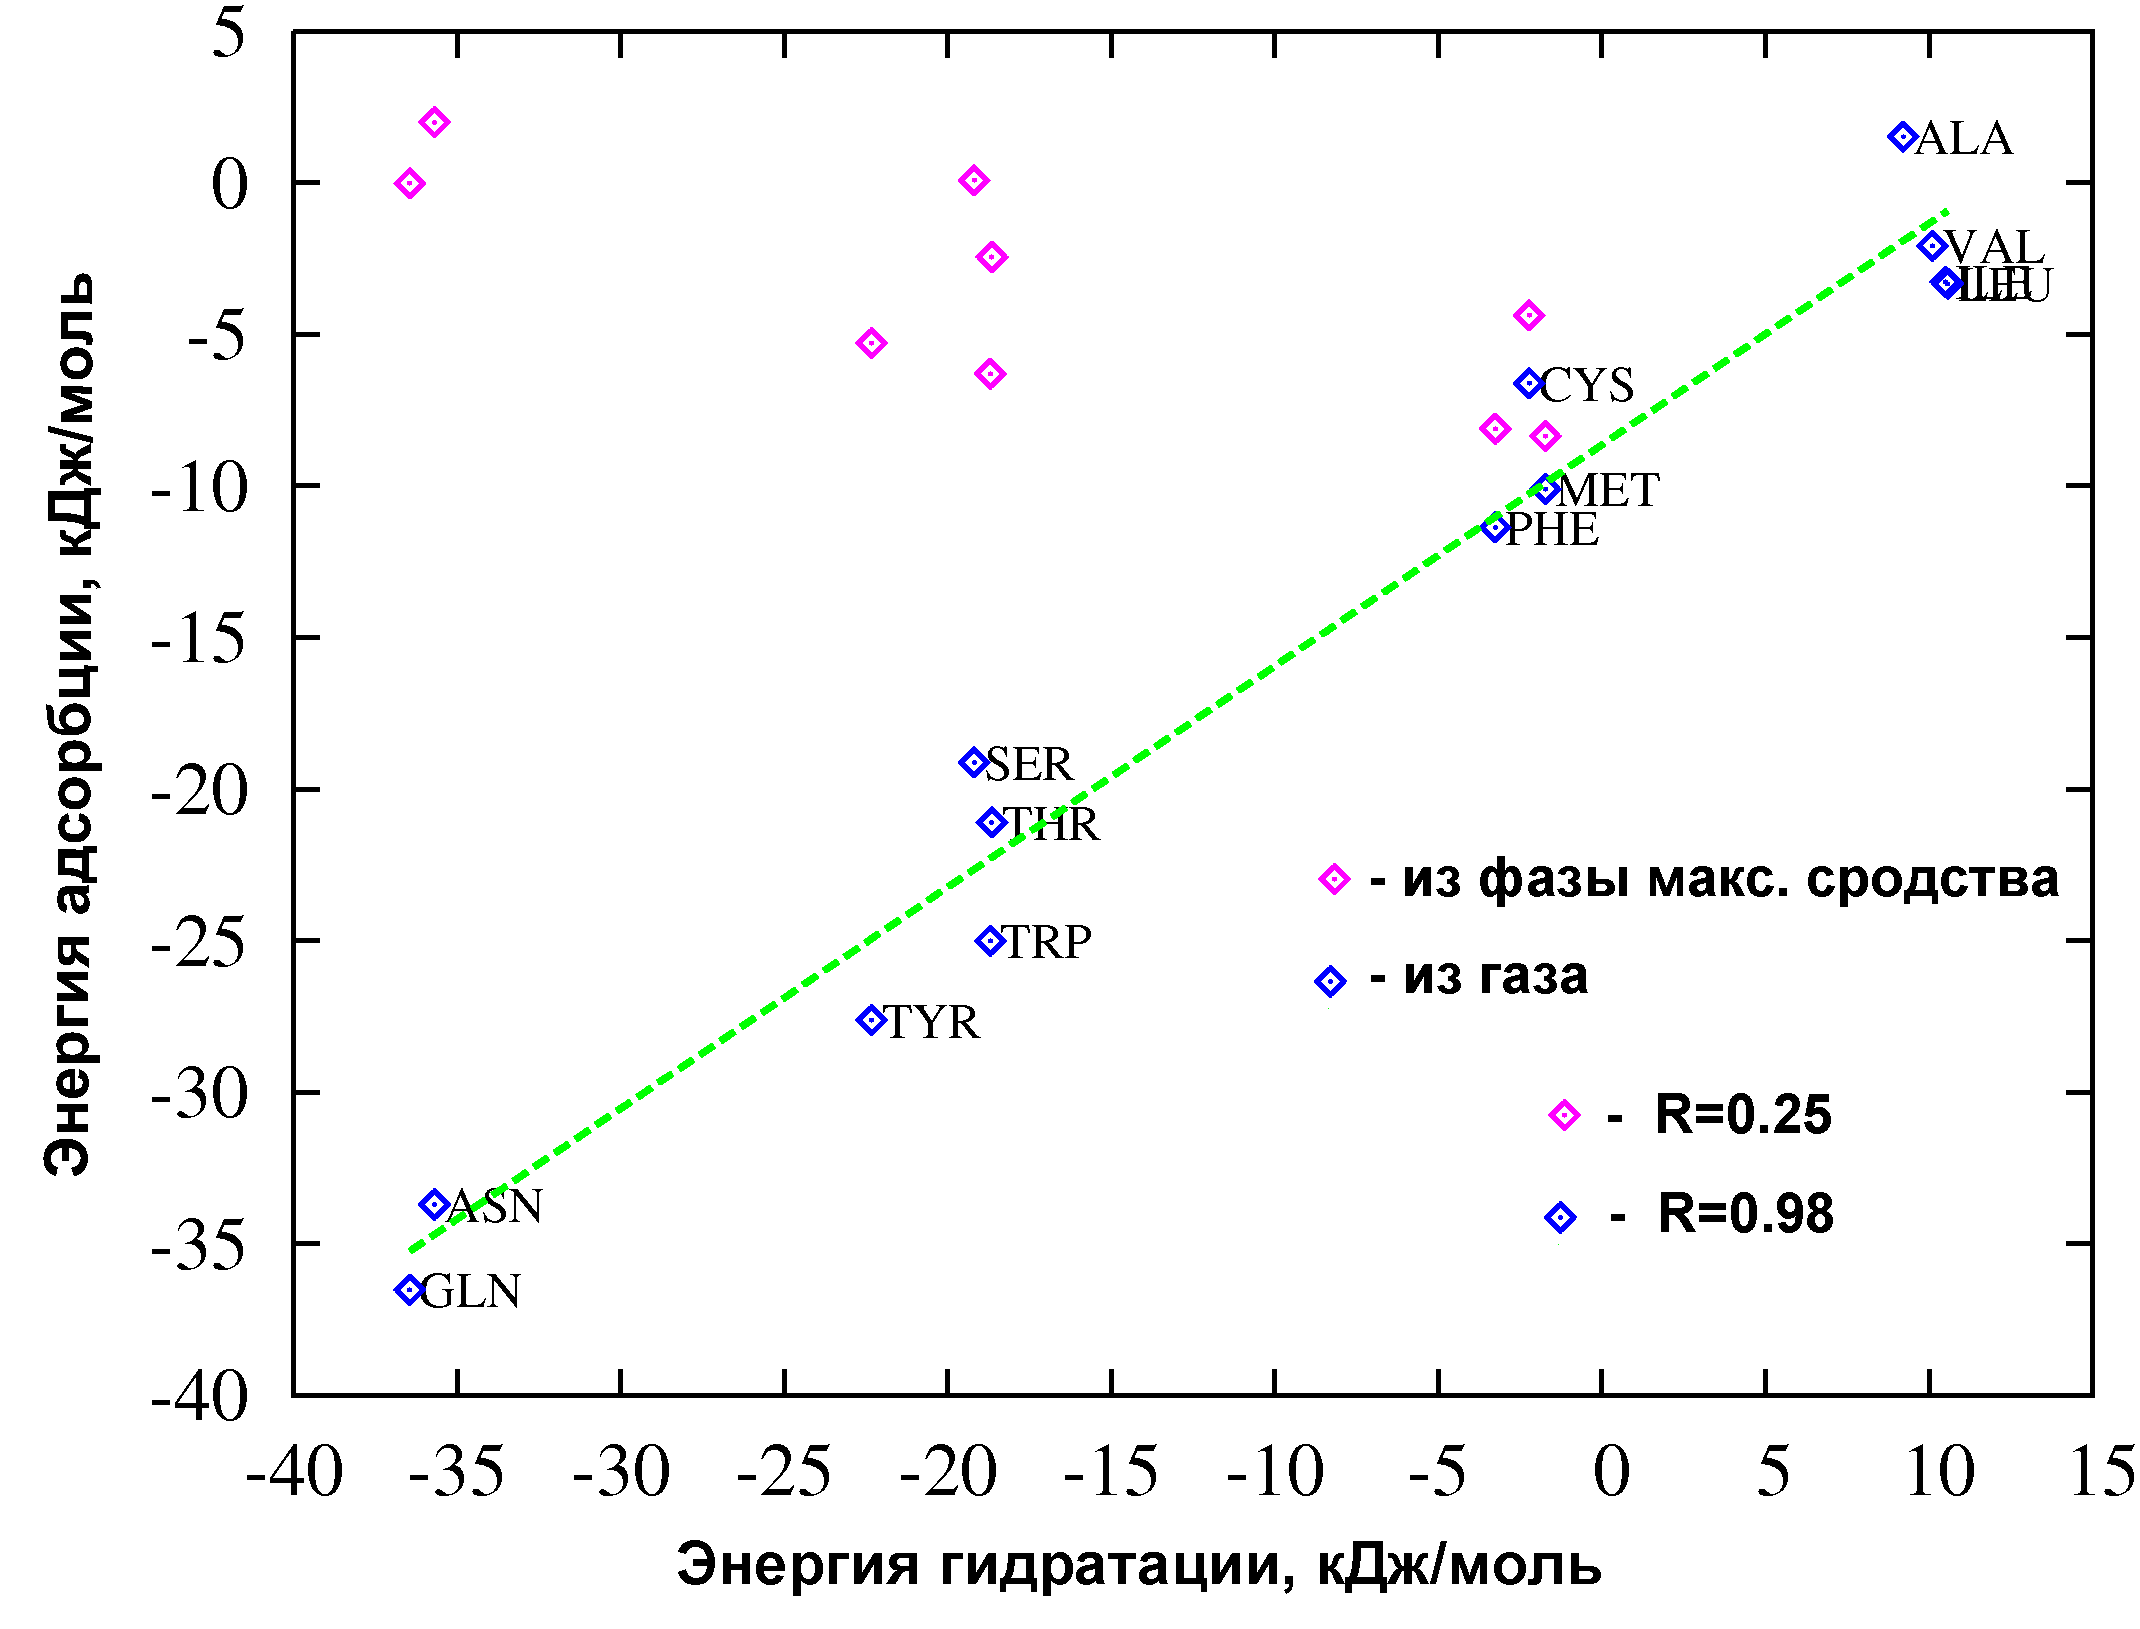
\includegraphics[width=10cm]{cor_ads_hydr_affin}
\caption{\label{cor_ads_hydr_affin} График корреляций между энергиями гидратации и адсорбции.}
\end{figure}


\subsection{\label{sec:comp_correl}Корреляционный анализ }
Поскольку на данный момент не существует систематических данных по экспериментальному измерению энергий адсорбции, изученных боковых цепей аминокислот, то представляется интересным провести анализ корреляций между полученными данными и статистическими шкалами предложенными в главе 4. Соответствующие коэффициенты корреляции, а также коэффициенты корреляции статистических шкал с экспериментальными, рассчитанные только для 13 исследованных соединений, представлены в таблице \ref{tab:comp_corr}. Как видно из таблицы, по коэффициентам корреляции шкала $G_{Gibbs}^{ads}$ достаточно хорошо совпадает со шкалой гидратации ($V>W$). Это вызвано тем, что для полярных гидрофильных молекул энергия адсорбции (глубина адсорбционного минимума) не сильно отличается от энергии гидратации. Для неполярных молекул такое утверждение не справедливо, энергия гидратации там плохо коррелирует с энергией адсорбции, однако, величины этих энергий не велики и коэффициент корреляции они портят не сильно. Демонстрация этого факта приведена на рис. \ref{cor_ads_hydr_affin}.

%\begin{turnpage}
\begin{table}
\caption{\label{tab:comp_corr} Коэффициенты корреляции энергий адсорбции ($G_{Gibbs}^{ads}$), полученных в результате численного моделирования и экспериментальных шкал  со статистическими данными, полученными в главе 4. Корреляции рассчитывались только для 13 незаряженных аминокислот.}

	\begin{tabular}{l|ccc|cc}
	        & ``10-20'' & ``50-60'' & ``95-105''& $G_{Gibbs}^{ads}$ & $G_{affin}^{ads}$\\
	   \hline
$G_{Gibbs}^{ads}$ & 0.48  &  0.88  & 0.7 & 1 & 0.17\\
$G_{affin}^{ads}$&     0.2         &  0.53         &  0.7     & 0.17  & 1\\
V>W&0.46&0.87&0.73 & 0.98 & 0.23 \\
CH>W&0.19&0.91&0.92 & 0.81 & 0.56\\
O>W&0.09&0.76&0.88 & 0.48 & 0.77\\


\end{tabular}

	
\end{table}
%\end{turnpage}
	 

\section{Выводы главы \ref{part3_free_energy}}

\textbf{Значимость и актуальность}\\
Рост возможностей современных компьютерных систем постепенно позволяет переходить на качественно новый уровень в моделировании молекулярных процессов: вычисления свободных энергий, энтропий и других термодинамических характеристик реальных молекулярных систем на основе их атомистических моделей с приемлемой точностью. Основные трудности таких вычислений связаны с (i) необходимостью осуществления обширной выборки состояний системы в различных статистически значимых конформациях, число которых быстро возрастает с увеличением сложности энергетического ландшафта системы, (ii) необходимостью понимания применимости существующих силовых полей, параметризованных по различным ``энергетическим'' характеристикам молекул, для вычислений такого рода, 
(iii) умением соотносить характеристики рассчитанные в системах небольшого размера с настоящими термодинамическими характеристиками и необходимостью разрабатывать соответствующие методы.
Особый интерес такие методы вызывают в связи с моделированием и построением моделей различных биологических структур (в частности белков), в самоорганизации которых важную роль играют гидрофобные взаимодействия, как раз носящие энтропийный, сильно статистический характер и, без адекватного описания которых на молекулярном уровне,
рассмотрение задач о самосборке и стабильности таких структур в компьютерном моделировании весьма сложно. Заметим, что выигрыш в свободной энергии при сворачивании белков весьма небольшой (10-20 ккал/моль), что накладывает дополнительные требования к качеству воспроизведения взаимодействий в моделировании. Короме того, поскольку биологические системы являются зачастую микрогетерогенными, (например, растворитель и ядро белка, актуальным является также корректное воспроизведение взаимодействий для отдельных молекул как в объёме фазы, так и на поверхности, что в свою очередь влияет на такую характеристику как поверхностное натяжение.
В данной работе освещён один из фундаментальных и одновременно методологических аспектов компьютерного моделирования белково-подобных систем, рассмотрено взаимодействие различных типов аминокислот с границей раздела фаз вода/воздух. Результаты работы с одной стороны дают фундаментальную информацию о взаимодействии аминокислот с поверхностью воды, с другой стороны предоставляют численные результаты для оценки точности широкоиспользуемых в настоящее время силовых полей и их совершенствования.

\textbf{Проведённые работы}\\
Была разработана методика моделирования, исследована структура (в том числе ориентационная) и характеристики водного слоя толщиной 4 нм. Разработана методика и вычислены профили свободной энергии для боковых цепей аминокислот вдоль нормали к границе водного слоя. Обсуждается вопрос о методах расчёта энергии адсорбции, предложено два метода и проведены оценки энергии адсорбции для боковых цепей аминокислот. Независимым способом путём ``выключения'' взаимодействия между молекулой и растворителем в объёме проведена оценка свободной энергии гидратации исследуемых молекул, проведено сравнение энергий получаемых двумя способами. На основании расчётов проведена оценка корреляций между энергиями гидратации и адсорбции (как абсолютных, так и относительно фазы максимального сродства), также проведена оценка корреляций шкал с результатами статистического анализа главы 4. 

\textbf{Положение работы в контексте аналогичных работ и новизна}\\
Расчёты свободных энергий гидратации для боковых цепей аминокислот были проведены целым рядом исследователей для различных силовых полей. В нескольких работах авторы очень внимательно относились к возможной зависимости параметров моделирования на получаемые результаты и получали результаты с достоверной оценкой погрешностей. Следует отметить, что данная тема является достаточно широко исследуемой в связи с вышеозвученными аргументами. Расчёт профилей свободной энергии для небольших молекул (в основном газов) на границе с водой проводился некоторыми исследователями, однако, на взгляд автора, в имеющихся работах выполнен достаточно небрежно. Что же касается систематического расчёта профилей свободной энергии для боковых цепей аминокислот на границе с водой, то таких работ найдено не было, поэтому можно утверждать, что данная работа выполнена впервые. Предложенный автором способ расчёта энергий адсорбции на основе профилей свободной энергии в купе с методом молекулярного моделирования также обладает новизной.




По результатам работы можно сделать следующие выводы, обладающие научной новизной:
\begin{itemize}
\item Профили средней силы для боковых цепей аминокислот на границе вода-воздух приблизительно одинаковы по форме: имеют область притяжения перед поверхностью Гиббса со стороны воздуха, и достаточно узкую (0.6-0.7 нм) область выталкивания за поверхностью Гиббса.
\item Вывод об одинаковой форме профилей средней силы на границе вода/воздух, по-видимому, можно обобщить на весть класс небольших незаряженных молекул.
\item В использованной модели, видимые поверхностные эффекты сольватации для боковых цепей аминокислот исчезают, когда центр масс молекулы погружён на 0.6-0.7 нм в воду по отношению к поверхности Гиббса, что может считаться эффективной глубиной границы раздела для маленьких молекул.
\item Профили свободной энергии для всех молекул обладают минимумом в районе границы раздела, который является результатом баланса между силами притяжения, доминирующими со стороны воздуха, и силами отталкивания, доминирующими со стороны воды, и имеющими энтропийную природу.
\item Глубина минимума свободной энергии находится в хорошей корреляции с энергией адсорбции, рассчитанной по методу Гиббса.
\item С высокой точностью вычислены энергии гидратации и адсорбции для 13 незаряженных веществ-аналогов боковых цепей аминокислот.
\item Показано, что энергия адсорбции из газовой фазы для выбранного набора боковых цепей аминокислот находиться в хорошей корреляции с энергией гидратации.
\item Энергия адсорбции относительно фазы максимального сродства не коррелирует с энергией гидратации и может использоваться как независимая термодинамическая характеристика молекул вещества.
\item Полученные данные для нескольких молекул согласуются с экспериментальными данными и могут применяться для совершенствования силовых полей, однако достоверных систематических данных по оценки энергии адсорбции для всей группы веществ на границе вода-воздух пока в литературе не обнаружено.
\end{itemize}


\subsection{Положения выносимые на защиту}
%положения выносимые на защиту
\begin{enumerate}
  \item Разработаны подходы позволяющие вычислять термодинамические параметры взаимодействия малых органических молекул с водой и ее поверхностью (свободную энергию гидратации и адсорбции) на основе их атомистических моделей.
  \item Систематическое завышение свободной энергии гидратации боковых цепей аминокислот современными силовыми полями (на 0.5 - 2 kT на аминокислоту) является одним из факторов гиперстабильности молекулярно-динамических моделей белков, свидетельствует о необходимости улучшения силовых полей биомакромолекул и молекул воды для моделирования фолдинга белков. 
\end{enumerate}           % Глава 3 - применение методов Enhanced sampling - свободные энергии

\chapter[Интегративное моделирование с применением данных экспериментов по футпринтингу ДНК]{Интегративное моделирование с применением данных экспериментов по футпринтингу ДНК\footnote{При подготовке данного раздела диссертации использованы следующие публикации, выполненные автором лично или в соавторстве, в которых, согласно Положению о присуждении ученых степеней в МГУ, отражены основные результаты, положения и выводы исследования: \cite{shaytan_hydroxyl-radical_2017,shaytan_structural_2018,armeev_modeling_2016}.}} \label{part5_hrf}
%NAR
%Nature protocols
В данной главе обсуждаются подходы по моделированию ДНК-белковых комплексов, основанные на использовании экспериментальных данных по футпринтингу ДНК гидроксильным радикалами. Излагаются основы метода футпринтинга ДНК. Описываются разработанные подходы по численному анализу экспериментальных данных и моделированию результатов футпринтинга на основе молекулярных моделей (реализованные в программном пакете HYDROID), которые позволяют использовать данные футпринтинга при построении молекулярных моделей. На основании разработанных подходов изучена конформация ДНК в нуклеосомах, разработан метод, позволяющий с точностью до одного нуклеотида определить позицию последовательности ДНК на нуклеосомном коре. Применение разработанных подходов интегративного моделирования продемонстрировано на примере создания структурной модели центромерной нуклеосомы пекарских дрожжей. Материалы данной главы основаны на следующих статьях \cite{shaytan_hydroxyl-radical_2017,shaytan_structural_2018,armeev_modeling_2016} и тезисах \cite{armeev_abstract_2019,armeev_integrative_2020}.


\section{Методы количественной обработки и структурной интерпретации экспериментов по расщеплению ДНК гидроксил радикалами с помощью программы HYDROID}
\textit{Содержание данной главы следует статье \cite{shaytan_structural_2018}}.


Метод гидроксильного футпринтинга (hydroxil-radical footprinting, HRF) является мощным методом исследования структур комплексов нуклеиновых кислот и белков в растворе с разрешением до одного нуклеотида. Чтобы использовать весь количественный потенциал HRF, мы описываем протокол для количественной оценки данных HRF и интеграции этих данных с атомистическими структурными моделями. Наш протокол, HYDroxyl-Radical Footprinting Interpretation for DNA (HYDROID) позволяет - анализировать данные HRF, полученные с помощью гель-электрофореза, - оценивать теоретические профили расщепления ДНК, полученные из молекулярных моделей, - визуализировать и сравнивать экспериментальные и теоретические профили расщепления. HYDROID полагается на новые алгоритмы аппроксимации данных и надежные подходы к обработке молекулярных моделей. HYDROID реализован на Python и обладает как возможность вызова из скриптов, так графического интерфейса. Этапы протокола HYDROID включают извлечение профилей дорожек из изображений геля, количественную оценку частоты расщепления ДНК по каждому нуклеотиду, теоретическую оценку частоты расщепления ДНК из атомистических структурных моделей с последующим сравнением экспериментальных и теоретических результатов. Примеры сценариев для каждого шага анализа и интерпретации данных HRF представлены для нескольких нуклеосомных систем; их можно легко адаптировать для анализа пользовательских данных. В качестве входного сигнала для HYDROID требуются изображения электрофоретических гелей продуктов реакции расщепления ДНК гидроксильными радикалами в полиакриламидном геле. Также может использоваться молекулярная модель комплекса ДНК-белок. Протокол HYDROID можно использовать для количественной оценки HRF на сегментах ДНК до 100 нуклеотидов на изображение геля. Кроме того протокол можно применять для анализа комплексов РНК-белок и свободных молекул РНК или ДНК в растворе. По сравнению с другими методами, HYDROID уникален своей способностью одновременно интегрировать данные HRF с анализом атомистических структурных моделей. HYDROID находится в свободном доступе по адресу \url{https://github.com/ncbi/HYDROID}. Выполнение полного протокола занимает примерно $\sim$ 3 часа. Пользователи должны быть знакомы с интерфейсом командной строки, языком сценариев Python и форматами файлов PDB. Также доступен графический пользовательский интерфейс с базовыми функциями (HYDROID\_GUI).


\subsection{Введение}
    Структурная характеристика комплексов нуклеиновая кислота-белок с высокой точностью необходима для нашего понимания функционирования генома, включая регуляцию экспрессии генов, транскрипцию, репликацию и репарацию ДНК. Хотя рентгеновская кристаллография остается золотым стандартом для определения структурных характеристик на атомистическом уровне, эта методика является сложной и часто не дает результатов из-за проблем с кристаллизацией. Методы ДНК-футпринтинга традиционно использовались как грубые, но универсальные и простые способы исследования взаимодействий ДНК-белок \textit{in vitro} \cite{tullius_physical_1989} и \textit{in vivo} \cite{adilakshmi_hydroxyl_2006,song_dnase-seq_2010}. В этих методах используются различные химические или ферментные агенты (например, ДНКаза I и гидроксильные радикалы) для расщепления ДНК в позициях, подверженных воздействию растворителя. Расположение этих положений может быть впоследствии идентифицировано с помощью гель-электрофореза при условии, что нити ДНК помечены радиоактивными или флуоресцентными метками на одном конце. Точность ферментативного расщепления ДНК ограничена стерическими эффектами и эффектами, специфичными для последовательности. С другой стороны, HRF является мощным методом, так как расщепление гидроксильными радикалами не имеет эффектов специфичных для последовательности, и обеспечивают высокое разрешение (вплоть до одного нуклеотида) из-за их малых размеров (см. \cite{jain_footprinting_2008-1} для подробного описания метода HRF).
    
    Основная интерпретация данных HRF часто выполняется качественно путем изучения соответствующих изображений электрофореза в полиакриламидном геле (ПААГЭ) ДНК или профилей интенсивности полос геля, полученных из этих изображений. Однако такой подход обычно не приводит к прямой трехмерной структурной интерпретации данных. Чтобы раскрыть весь потенциал этих высококачественных экспериментальных данных, необходимо выполнить две задачи: 1) количественную оценка фактических частот расщепления ДНК для каждого положения нуклеотида из данных ПААГЭ и 2) оценку частот расщепления ДНК из соответствующих атомистических молекулярных моделей. Вместе эти два компонента анализа позволяют интерпретировать данные HRF на более продвинутом уровне и позволяют включать данные в конвейеры молекулярного моделирования (рис. \ref{fig:p5_1_f1}) \cite{armeev_modeling_2016}. Используя такой подход, атомистические структурные модели высокого разрешения комплексов ДНК-белок могут быть проверены и/или уточнены с использованием экспериментальных данных HRF.



\begin{figure} [H]
    \centering
    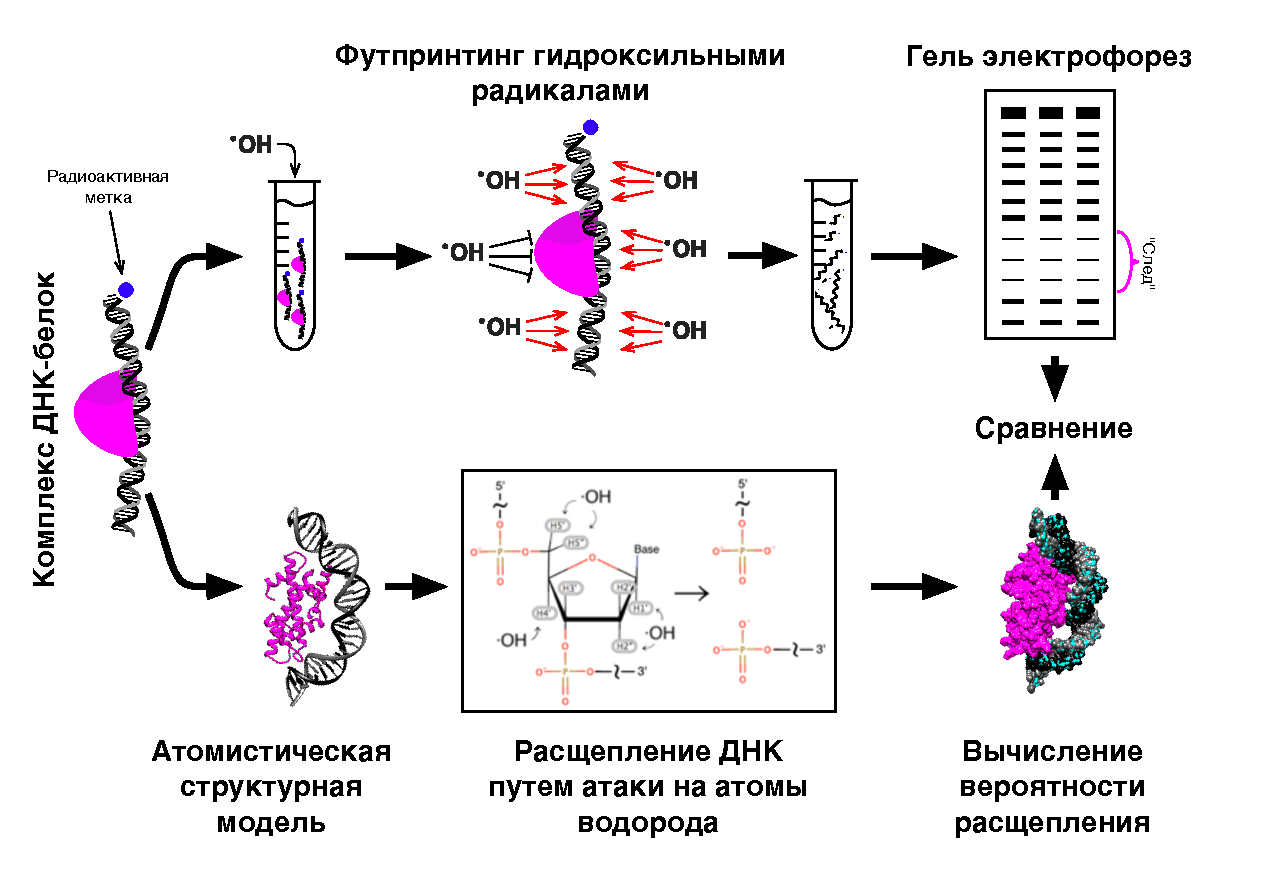
\includegraphics[width=\textwidth]{images/p5/part5_1_np/p5_1_f1.pdf}
    \caption[Футпринтинг комплексов ДНК-белок гидроксильными радикалами и структурная интерпретация экспериментальных данных.]{\textbf{Футпринтинг комплексов ДНК-белок гидроксильными радикалами и структурная интерпретация экспериментальных данных.} На схематической диаграмме изложены основные идеи использования HRF для выяснения структуры комплексов ДНК-белок. Вверху: комплексы ДНК-белок восстанавливаются на радиоактивно меченной ДНК и подвергаются расщеплению гидроксильными радикалами; гидроксильные радикалы расщепляют нити ДНК на участках, не защищенных белком, в режиме кинетики одиночных расщеплений (по одному разрезу на нить); Репертуар расщепленных фрагментов ДНК анализируется с помощью денатурирующего гель-электрофореза, и становятся очевидными положения в последовательности ДНК, защищенных белком. Внизу: атомистические структурные модели могут использоваться для прогнозирования профилей футпринтинга; частота расщепления зависит от доступности атомов водорода дезоксирибозы; сравнение предсказанных и экспериментальных результатов может быть использовано для уточнения или проверки структурных моделей.}
    \label{fig:p5_1_f1}
\end{figure}

\subsection{Разработка протокола}

    Теоретическая основа для количественной оценки экспериментальных данных футпринтинга гидроксильными радикалами была предложена ранее \cite{balasubramanian_dna_1998,shadle_quantitative_1997,das_safa_2005,bishop_map_2011}. Однако, столкнувшись с практической необходимостью структурной интерпретации данных HRF для комплексов ДНК-белок в наших недавних исследованиях \cite{shaytan_hydroxyl-radical_2017,xiao_molecular_2017}, мы поняли, что не существует простого протокола и программного обеспечения как для количественной оценки данных HRF, так и для анализа атомистической структуры. Ранее описанные подходы \cite{shadle_quantitative_1997,das_safa_2005}, которые использовались для количественной оценки результатов ПААГЭ или расчетов доступной для растворителя площади поверхности для анализа трехмерной структуры, утратили совместимость с современными компьютерными платформами или не имеют воспроизводимых примеров данных для их повторной реализации и проверки. Чтобы удовлетворить эту потребность, мы разработали свободно доступное программное обеспечение и здесь предоставляем пошаговые инструкции по его использованию.

    Мы представляем протокол и программный пакет HYDROID (HYDroxyl-Radical fOotprinting Interpretation for DNA). HYDROID обеспечивает: количественный анализ данных HRF с разрешением в один нуклеотид, оценку частот расщепления ДНК по кристаллическим структурам или атомистическим молекулярным моделям, сравнение и интеграцию этих подходов. HYDROID написан на Python и использует бесплатные кроссплатформенные компоненты ImageJ для анализа изображений \cite{schneider_nih_2012} и библиотеку FreeSASA для расчета площади поверхности \cite{mitternacht_freesasa_2016}. Кросс-платформенный и надежный характер структуры HYDROID поддерживается этими хорошо обслуживаемыми, регулярно обновляемыми и тщательно тестируемыми базовыми технологиями. Протокол HYDROID состоит из двух библиотек, HYDROIDexp (анализ и визуализация экспериментальных данных) и HYDROIDpred (анализ структуры) вместе с набором примеров и пошаговыми инструкциями. HYDROID количественно оценивает экспериментальные профили дорожек ПААГЭ с помощью аппроксимации данных с использованием различных функций и ограничений при проведении аппроксимации. Пакет оценивает теоретические профили частоты (интенсивности) расщепления ДНК на основе атомистических трехмерных структур путем вычисления доступной для растворителя площади поверхности атомов водорода дезоксирибозы. Чтобы ознакомиться с протоколом HYDROID, мы создали видеоурок по адресу \url{https://ncbi.github.io/HYDROID/docs/video.html}. Протокол успешно применялся в двух исследованиях \cite{shaytan_hydroxyl-radical_2017,xiao_molecular_2017}.

\subsection{Применение метода}

    HYDROID - это надежный, но гибкий инструмент для анализа и интерпретации экспериментов по футпринтингу ДНК. Он одновременно сочетает в себе функциональность для количественной оценки данных ПААГЭ продуктов футпринтинга (HYDROIDexp) и оценки профилей расщепления ДНК в ходе гидроксильного футпринтинга из экспериментальных структур или молекулярных моделей (HYDROIDpred).

    Ранее мы применили подход HYDROID для изучения центромерных нуклеосом дрожжей и их комплексов с белком CENP-C \cite{shaytan_hydroxyl-radical_2017,xiao_molecular_2017}. Высококачественный анализ экспериментальных данных HRF с помощью HYDROID позволил нам точно определить положение ДНК на октамере гистонов, построить атомистическую модель центромерной нуклеосомы, воссозданной на определенной последовательности ДНК, и идентифицировать сайты взаимодействий белка CENP-C с нуклеосомой.

    В этом разделе подход HYDROID был протестирован и подтвержден с использованием нескольких наборов экспериментальных данных по комплексам ДНК-белок. Мы проанализировали влияние различных параметров на производительность HYDROID и дали рекомендации относительно того, какие параметры следует использовать при анализе комплексов ДНК-белок. В разделе ``Экспериментальный дизайн'' представлены дополнительные сведения, соответствующие примеры и рекомендации.

    Основные функции модулей HYDROID можно легко адаптировать и использовать для более широкого спектра приложений. В частности, модуль HYDROIDexp сам по себе может применяться для анализа данных гель-электрофореза нуклеиновых кислот любого типа, обеспечивая точное количественное определение интенсивности полос. Алгоритмы аппроксимации полос, разработанные в HYDROIDexp, в целом могут быть адаптированы для анализа данных капиллярного электрофореза.

    Модуль HYDROIDpred в его нынешнем виде способен анализировать доступность атомов водорода рибозы/дезоксирибозы с использованием подхода вычисления поверхности доступной растворителю H-SASA для свободной ДНК или РНК или в комплексе с белками. Мы не проводили обширных испытаний подхода H-SASA для оценки профилей частоты расщепления в случаях, отличных от комплексов ДНК-белок. Однако другие исследования ранее показали, что оценка профилей H-SASA для определенных атомов водорода в нативной РНК или ДНК может быть аналогичным образом использована для оценки паттернов расщепления HRF \cite{bishop_map_2011,ingle_chemical_2014}. В таких случаях мы рекомендуем ознакомиться с указанными выше ссылками и указать в скрипте HYDROIDpred, какие атомы водорода следует учитывать для анализа. Учитывая важность метода HRF для анализа третичной структуры РНК и РНК-белковых комплексов \cite{costa_probing_2014,hampel_time-resolved_2001,nilsen_mapping_2014}, мы ожидаем, что части пакета HYDROID будут полезны для этой цели и потенциально могут быть включены в конвейеры предсказания структуры РНК \cite{ding_three-dimensional_2012,tian_rna_2016}.


\subsection{Сравнение с другими методами}

    Уникальной характеристикой HYDROID является интеграция количественной оценки экспериментальных данных HRF и анализа атомистической трехмерной структуры в одном пакете. Преимущества функциональности, предоставляемой отдельными компонентами HYDROID (HYDROIDexp и HYDROIDpred), обсуждаются ниже.
    
    Некоторые автономные программы были разработаны на протяжении многих лет для решения задач количественной оценки гелей в экспериментах HRF, такие как GelExplorer \cite{shadle_quantitative_1997} или SAFA \cite{das_safa_2005}. Однако одним препятствием при использовании этих программ в настоящее время является то, что они не обновлялись в течение некоторого времени и не совместимы с современными компьютерными системами. Дополнительные преимущества библиотеки HYDROIDexp включают возможность выбора гауссовой или лоренцевой формы полос и множество алгоритмов аппроксимации с ограничениями на вариации параметров. Библиотека HYDROIDexp также включает инструменты, совместимые с Python, для построения профилей вдоль последовательности ДНК. Это бесплатное программное обеспечение, которое можно повторно использовать в других проектах.

    Что касается теоретической оценки профилей расщепления ДНК из трехмерных структур, HYDROIDpred в настоящее время является единственным доступным решением. Он основан на вычислении доступности атомов водорода через библиотеку FreeSASA, которая является быстрой и бесплатной в использовании. HYDROIDprep расширяет ее, предоставляя для расчетов тщательно подобранные наборы атомных радиусов. Ранее сообщалось об альтернативном подходе (подход RADACK), который пытается учесть контролируемую диффузией природу реакции атаки гидроксильных радикалов и общую геометрию молекулы с помощью стохастического моделирования \cite{begusova_radack_2001}. Однако в настоящее время нет общедоступного программного обеспечения, реализующего подход RADACK.

\subsection{Преимущества и ограничения}

    Основным преимуществом HYDROID является его конструкция 2-в-1, предоставляющая пользователю возможность одновременно количественно оценивать экспериментальные данные HRF и сравнивать их с атомистическими структурными моделями комплекса белок-нуклеиновая кислота, если они доступны. Оба компонента HYDROID, реализующие эти функции, имеют свои преимущества. В частности, преимущества HYDROIDexp включают его кроссплатформенный характер (работает в Linux, Windows, MacOS) и одновременную реализацию ряда алгоритмов аппроксимации профиля HRF (формы полос Гаусса или Лоренца в сочетании с несколькими алгоритмами аппроксимации с ограничениями). Алгоритмы аппроксимации с ограничениями хорошо работают при деконволюции сигнала от частично перекрывающихся полос геля. Преимущества HYDROIDpred включают его бесплатную природу без каких-либо патентованных или лицензионных программных компонентов, а также тщательно отобранные и проверенные наборы параметров (радиус зонда, размеры атомов), которые можно использовать для получения значимых оценок профиля расщепления ДНК на основе молекулярных моделей. Алгоритм HYDROIDpred основан на оценке доступной для растворителя области атомов водорода дезоксирибозы. Этот подход не может напрямую объяснить кинетику диффузии гидроксильных радикалов (см. Раздел ``Схема эксперимента'' для дальнейшего обсуждения). Следовательно, следует проявлять осторожность при сравнении точных форм экспериментальных и теоретических профилей расщепления.

    Для подхода HYDROIDpred на вход должны быть поданы PDB-структуры с атомами водорода. Предлагаемый алгоритм добавления атомов водорода (шаг 23) в настоящее время работает только в Linux или Mac.


\subsection{Обзор протокола HYDROID}

    HYDROID состоит из протокола и программного пакета, написанного на языке Python, который вместе с другими компонентами (ImageJ и FreeSASA) представляет собой надежную основу для анализа и интерпретации экспериментальных данных футпринтинга гидроксильными радикалами ДНК-белковых комплексов. Протокол также может применяться для анализа комплексов РНК-белок, а также свободных молекул РНК/ДНК в растворе. Пакет программного обеспечения HYDROID можно легко установить в операционных системах Linux, Mac или Windows. Он состоит из двух дополнительных конвейеров (и соответствующих программных библиотек) HYDROIDexp и HYDROIDpred. Конвейер HYDROIDexp используется для анализа изображений геля ПААГЭ для получения значений частоты расщепления ДНК для каждой позиции на исследуемой последовательности ДНК (рис. \ref{fig:p5_1_f2}, вверху). Конвейер HYDROIDpred используется для выполнения теоретических расчетов частоты расщепления ДНК на основе трехмерной атомистической структуры или молекулярной модели комплекса ДНК-белок (рис. \ref{fig:p5_1_f2}, внизу). Расчеты частоты расщепления выполняются путем расчета доступной для растворителя площади поверхности атомов водорода дезоксирибозы (которые атакуются гидроксильными радикалами и вызывают расщепление ДНК) для каждого нуклеотида (профили H-SASA). Профили H-SASA позволяют оценить ожидаемую частоту расщепления ДНК. Сравнение и интегрирование экспериментальных и теоретических профилей можно в дальнейшем использовать для интерпретации экспериментальных данных и/или уточнения молекулярной модели. Основные программные функции, реализованные в пакете HYDROID, перечислены в таблице \ref{tab:p5_t1}. Они предназначены для запуска из сценария Python, а некоторые функции имеют интерактивный графический интерфейс пользователя. В пакете HYDROID полнофункциональные примеры данных HRF и анализа трехмерной структуры представлены в виде тщательно аннотированных скриптов Python. Эти примеры можно легко загрузить, и они служат в качестве изменяемых шаблонов для анализа пользовательских данных (см. ПРОЦЕДУРА и ОЖИДАЕМЫЕ РЕЗУЛЬТАТЫ). Ниже мы описываем методологию, лежащую в основе ключевых этапов структуры HYDROID. Видеоиллюстрации каждого этапа доступны по адресу \url{https://ncbi.github.io/HYDROID/docs/video.html}.

\subsection{Конвейер HYDROIDexp}
 Конвейер HYDROIDexp требует в качестве входных данных изображение геля ПААГЭ с дорожками для продуктов HRF одной из нитей ДНК и соседних дорожек с продуктами реакций секвенирования ДНК для той же цепи. Конвейер дает значения относительной частоты расщепления ДНК (также называемые значениями интенсивности расщепления ДНК) вдоль последовательности ДНК. Этот конвейер можно применять параллельно к нескольким образцам, которые были обработаны на одном и том же геле. Конвейер состоит из пяти этапов. См. Диаграмму рабочего процесса на рисунке \ref{fig:p5_1_f2}.


\begin{figure} [H]
    \centering
    \includegraphics[width=\textwidth]{images/p5/part5_1_np/p5_1_f2.pdf}
    \caption[Конвейеры данных в HYDROID]{Конвейеры данных в HYDROID. Схематическая диаграмма для анализа экспериментальных данных по футпринтингу гидроксильными радикалами (вверху, HYDROIDexp). Теоретическая оценка профилей расщепления ДНК по молекулярным структурам (внизу, HYDROIDpred). Шаги и этапы процедуры аннотированы на схеме. Конвейер HYDROIDexp состоит из пяти этапов (отмечены синим цветом): этап 1 - профили дорожек в виде файлов данных извлекаются из изображения ПААГЭ, этап 2 - положения полос/пиков назначаются полуавтоматически на профилях дорожек, этап 3 - соответствие между полосами геля и последовательностью ДНК устанавливается, этап 4 - математическая модель подбирается для описания формы профиля дорожки с помощью функций Гаусса или Лоренца, этап 5 - интенсивности отдельных полос (частоты расщепления ДНК) извлекаются из модели. Конвейер HYDROIDpred состоит из двух этапов: этап 1 - загружается файл PDB интересующей системы и добавление атомов водорода к атомистической структуре при необходимости, этап 2 - профили доступности ДНК рассчитываются путем оценки доступной для растворителя области атомов водорода дезоксирибозы (H-SASA). Наконец, можно сравнить наборы теоретических и экспериментальных данных.}
    \label{fig:p5_1_f2}
\end{figure}



    \emph{Этап 1: Извлечение профилей дорожек геля}. Экспериментальные профили дорожек извлекаются из изображения геля. Экспериментальный профиль интенсивности полосы геля (профиль полосы) в дальнейшем определяется как массив значений интенсивности на изображении геля вдоль указанной полосы гель-электрофореза (в направлении миграции ДНК по гелю). Функции HYDROID считывают данные экспериментального профиля гелевой дорожки, сохраненные в виде столбцов чисел в текстовых файлах. Для получения ``цифровых'' экспериментальных профилей дорожек из изображений гелей ПААГЭ мы предлагаем использовать программное обеспечение ImageJ \cite{schneider_nih_2012} с плагином Bio-Formats \cite{linkert_metadata_2010} везде, где это необходимо для открытия файлов определенных форматов изображений гелей. 
    %Во вставке 2 приведены подробные инструкции по извлечению профилей полос в совместимом текстовом файле табличного формата из изображения СТРАНИЦЫ с помощью ImageJ. 
    Чтобы HYDROID мог считывать данные из сгенерированного файла, необходимо указать отдельный текстовый файл конфигурации, в котором указываются имена дорожек и соответствующие имена столбцов в сгенерированном файле.
    %(см. Блок 3 для более подробной информации о форматах входных файлов для HYDROIDexp. ).

    \emph{Этап 2: Назначение отдельных полос/пиков на геле}. Положение отдельных полос геля идентифицируется на профиле полосы геля с помощью полуавтоматического интерактивного алгоритма. Для деконволюции профиля полосы в набор вкладов от отдельных полос, сначала нужно знать количество и приблизительное расположение полос на профиле дорожки. Каждая полоса обычно соответствует локальному пику на профиле дорожки. Полуавтоматический интерактивный алгоритм, реализованный в
     функции \textit{assign\_peaks\_interactive} в HYDROID, открывает графическое окно и позволяет пользователю изменять параметры процедуры поиска пиков до тех пор, пока все необходимые пики не будут правильно идентифицированы по оценке пользователя. Алгоритм поиска пиков основан на библиотеке PeakUtils Python.
      Алгоритм регулируется двумя параметрами: относительной известностью пиков (параметр пикового порога - будут обнаружены только пики с амплитудой выше порога) и минимальным расстоянием между пиками. Алгоритм поиска пиков разделяет профиль полосы на несколько сегментов и позволяет пользователю выбирать минимальное расстояние между пиками для самого левого и самого правого сегментов (параметры \textit{min\_dist\_left} и \textit{min\_dist\_right}); значения в промежуточных сегментах затем выводятся с использованием линейной интерполяции. Если некоторые полосы перекрываются до такой степени, что пики не могут быть идентифицированы на профиле полосы или интенсивность полосы очень мала, в HYDROID реализована опция интерполяции пиков, чтобы попытаться вывести их положения из известных положений и расстояний между соседними группами, которые более заметны. Наконец, положения пиков можно указать вручную в файле конфигурации.

    \emph{Этап 3: Привязка пиков HRF к последовательности ДНК}. Каждую полосу на дорожке геля HRF (которая эквивалентна пику на профиле дорожки HRF) можно отнести к определенному положению в последовательности ДНК путем сравнения дорожек геля HRF с дорожками с продуктами реакций секвенирования ДНК для тех же ДНК. В HYDROID функция \textit{call\_peaks\_interactive} позволяет интерактивно строить профиль дорожки HRF вместе с профилями реакций секвенирования ДНК и последовательностью ДНК. Визуально сравнивая их с последовательностью ДНК, пользователь может указать местоположение любого одиночного пика на профиле и его соответствующее положение на последовательности ДНК. Это позволяет установить соответствие между всеми полосами и положениями в последовательности ДНК.

    \emph{Этап 4: Аппроксимация профилей интенсивности дорожек.} Математические модели, описывающие распределение интенсивности каждой полосы с помощью функций Гаусса или Лоренца, подгоняются к данным профиля полосы с помощью функции \textit{fit\_peaks}. Эта процедура позволяет вам провести деконволюцию необработанного экспериментального профиля HRF на вклады отдельных полос геля, тем самым должным образом принимая во внимание такие эффекты, как частичное перекрытие сигналов полос и неравномерная ширина полосы вдоль полосы геля 
    %(см. Вставку 4 для математических деталей алгоритма). 
    Известно, что эта процедура подвержена от переобучению, если на алгоритм подгонки не накладываются дополнительные ограничения \cite{takamoto_semi-automated_2004}. В HYDROID реализован ряд различных вариантов подгонки с ограничениями, перечисленных в Таблице \ref{tab:p5_t2}. См. Раздел ``Проблемы при экспериментальной количественной оценке профилей HRF'' для обсуждения дополнительных деталей.

    Чтобы оценить качество подгонки экспериментального профиля полосы с помощью модели, HYDROID предоставляет несколько критериев оценки: RMSD - среднеквадратичное отклонение между экспериментальными и прогнозируемыми значениями модели, относительное RMSD - вариация последнего, где отклонение в каждой точке выражается как часть экспериментального значения, и коэффициент корреляции Пирсона между экспериментальными и прогнозируемыми значениями.

    Значения частоты расщепления ДНК (общие площади под пиками на профиле дорожек) оценивают методом нелинейной аппроксимации методом наименьших квадратов. Для каждого пика площадь рассчитывается под сегментом кривой, который включает этот пик. Сегмент определяется серединами между положением данного пика (положением его максимума) и положением пиков его соседей слева и справа. Относительные различия в значениях прокси-площади, определенных для экспериментального профиля дорожки, по сравнению с профилем подобранной модели, используются как оценки неопределенности и называются ``относительными ошибками площади пика''. Максимальная относительная ошибка площади пика среди всех пиков, а также среднеквадратическое значение (``RMSD относительной площади пика'') вычисляются в HYDROID.
    
    \emph{Этап 5: Расчет частоты расщепления ДНК.} Частота расщепления ДНК для каждой позиции на ДНК вычисляется как площадь под гауссианой/лоренцевой кривой, описывающей соответствующую полосу. Значения профиля частоты расщепления ДНК отображаются вдоль последовательности ДНК.
    
    \subsection{Конвейер HYDROIDpred}
     Теоретический расчет профилей расщепления ДНК с помощью HYDROID основан на анализе трехмерных атомистических структур комплексов белок-ДНК и оценке доступности атомов водорода дезоксирибозы для гидроксильных радикалов. Трехмерные координаты можно получить с помощью рентгеновской кристаллографии или молекулярного моделирования (моделирование по гомологии, интегративное моделирование, докинг и т. д.). Доступная для растворителя площадь поверхности атомов водорода дезоксирибозы рассчитывается для каждого нуклеотида в молекуле ДНК структурного комплекса, что приводит к двум профилям H-SASA, по одному для каждой цепи (в случае, если протокол применяется к РНК, это приведет к одному профилю H-SASA). Он дает оценочные значения относительной частоты расщепления ДНК. Конвейер состоит из трех основных этапов.
    
    \textit{\emph{Этап 1:}Приготовление атомистической модели комплекса ДНК-белок с известными положениями атомов водорода.} Важным шагом является определение положений атомов водорода, если они отсутствуют в исходной структуре. Небольшие различия в положениях атомов водорода (например, разные параметры длины для связей C-X) могут повлиять на величину оцененных профилей (см. Подробное обсуждение в разделе ``Проблемы оценки теоретических частотных профилей расщепления ДНК из атомистических структур''). Программа REDUCE \cite{word_asparagine_1999} из пакета AmberTools 17 \cite{case_amber_nodate} с расстояниями связей X-H, полученными из  положений ядер атомов, может использоваться при добавлении атомов водорода в рентгеновские структуры.
    
    \emph{Этап 2:} \textit{Оценка теоретической частоты расщепления ДНК.} Теоретические профили частоты расщепления ДНК оцениваются путем расчета доступной для растворителя площади поверхности атомов водорода дезоксирибозы (профили H-SASA) с помощью функции get\_DNA\_H\_SASA, которая использует библиотеку FreeSASA \cite{mitternacht_freesasa_2016}. Алгоритм Ли-Ричардса используется \cite{lee_interpretation_1971} в FreeSASA с точностью до 200 срезов на атом по умолчанию. Для расчета SASA могут применяться другие радиусы зонда, по умолчанию 1,4\AA. HYDROID реализует три набора атомных радиусов для расчетов H-SASA: a) радиусы FreeSASA по умолчанию, б) значения радиусов из силового поля CHARMM36 \cite{best_optimization_2012} и в) значения радиусов из силового поля AMBER ff10 (parm10) \cite{case_amber_nodate}. Последние два получены из параметров rmin ван-дер-Ваальса (расстояние/радиус, при котором энергия Леннарда-Джонса имеет минимум) соответствующих силовых полей. Затем выполняется визуализация рассчитанных профилей (см. Визуализация и сравнение данных ниже).
    
    
    \subsection{Визуализация и сравнение данных}
    
    Для визуализации и сравнения профиля частоты расщепления ДНК HYDROID включает модуль построения графиков (\textit{plot\_prof\_on\_seq}) на основе библиотеки Matplotlib \cite{hunter_matplotlib_2007}. Этот модуль может одновременно строить несколько профилей вместе с последовательностью ДНК и позволяет использовать несколько методов нормализации (для приведения профилей к одному масштабу). Реализованы некоторые тривиальные методы нормализации, такие как деление каждого профиля на его максимальное значение (``every\_method'') или деление обоих профилей на их максимальное общее значение (``together\_method''). Кроме того, ``метод подгонки'' выполняет линейную регрессию без свободного члена между значениями профиля и изменяет их масштаб максимизируя взаимное максимальное соответствие. Использование линейной регрессии без свободного члена соответствует физическому требованию, согласно которому позиции, недоступные для расщепления, должны иметь нулевые значения на обоих профилях.

    Кроме того, мы реализовали метод моделирования профилей полос геля и изображений геля из профилей частоты расщепления (функция \textit{simulate\_gel}). Эта функция полезна для изучения ожидаемой формы профилей гелевых полос (и, следовательно, разрешения профиля в конкретной интересующей области ДНК) и планирования экспериментов. Модель подвижности ДНК Огстона используется для моделирования подвижности ДНК в геле \cite{slater_dna_2001}.
    


\begin{table}[h!]
    \centering
    \begin{tabularx}{\textwidth}{|X|X|}
        \hline
        \multicolumn{2}{|l|}{\textbf{Библиотека HYDROIDexp}} \\
        \hline
        assign\_peaks\_interactive & Предоставляет интерактивный интерфейс для полуавтоматического алгоритма, используемого для определения положения пиков на профилях гелевых дорожек.\\
        \hline
        call\_peaks\_interactive & Предоставляет интерактивный интерфейс для назначения индивидуальных пиков относительно положения последовательности ДНК.\\
        \hline
        fit\_peaks & Основная функция, которая подгоняет математическую модель профиля гелевой дорожки и оценивает интенсивность расщепления ДНК.\\
        \hline
        plot\_prof\_on\_seq & Строит любой профиль данных по последовательности ДНК и позволяет нормализовать и подгонять два или более профилей.\\
        \hline
        simulate\_gel & Имитирует форму профиля полосы геля и выводит изображение полосы геля на основе профиля H-SASA.\\
        \hline
        \multicolumn{2}{l|}{\textbf{Библиотека HYDROIDpred}} \\
        \hline
        get\_DNA\_H\_SASA & Оценивает теоретические профили расщепления ДНК (профили H-SASA) по структуре ДНК-белка.\\
        \hline
    \end{tabularx}
    \caption{Основные функции HYDROID и их описание.}
    \label{tab:p5_t1}
\end{table}



\begin{table}[h!]
    \centering
    \begin{tabularx}{\textwidth}{|X|X|}
        \hline
        Тип ограничения (аббревиатура) & Описание \\
        \hline
        dSIGMA>=0 & Ширина пика $\sigma$ не должна уменьшаться с увеличением D, положения пика (то есть от начала геля до конца). Это значительно повышает стабильность решения и предотвращает переобучение. \\
        \hline
        SIGMA<2*dD & Ширина пика $\sigma$ не может превышать удвоенное расстояние между данным пиком/полосой и последующим пиком (dD). Подразумевает автоматически ``dSIGMA> = 0''. \\
        \hline
        SIGMA=k*D+b & Ширина пика $\sigma$ линейно связана с положением пика (D). Это эффективно устанавливает линейную зависимость между шириной полосы и ее подвижностью. \\
        \hline
        log(SIGMA)=P2(log(M)) & Логарифм ширины пика $\sigma$ пропорционален логарифму числа нуклеотидов в ДНК, M, (или ее молекулярной массе) через полином второй степени. Оптимальные коэффициенты полинома определяются при подгонке: $\sigma_i = e^{a*(log M_i)^2 +b* log M_i +c}$) \\
        \hline
        SAFA & Ограничения, реализованные в программе SAFA \cite{das_safa_2005}, ширина пика связана с положением соседних пиков через $\sigma_i = \sigma_0 + k * \frac{D_{i + 1}-D_i}{2}$\\
        \hline
    \end{tabularx}
    \caption{Список ограничений при подгонке моделей, доступные в HYDROID.}
    \label{tab:p5_t2}
\end{table}


\subsection{Планирование экспериментов}
    
    \subsubsection{Метод HRF и интерпретация данных}
     В методе HRF используются гидроксильные радикалы, образованные в результате реакции Фентона или облучения, для расщепления цепей ДНК в доступных для растворителя участках \cite{jain_footprinting_2008-1}. Химический процесс, лежащий в основе, следующий: гидроксильный радикал атакует атомы водорода дезоксирибозы, что приводит к отщеплению водорода и последующему расщеплению основной цепи (рис. \ref{fig:p5_1_f1}). Основными продуктами этого химического расщепления являются две цепи, оканчивающиеся 3$^\prime$ и 5$^\prime$ фосфатами, которые примыкают к атакованному нуклеотиду в исходной цепи ДНК. Анализ продуктов расщепления ДНК обычно проводят с использованием денатурирующего электрофореза в полиакриламидном геле (ПААГЭ) предварительно радиоактивно/флуоресцентно меченой цепи (нитей) ДНК. Обычно рекомендуется радиоактивное мечение 5$^\prime$-конца ДНК \cite{jain_footprinting_2008-1}. В пределах кинетики единичного попадания (один разрез на цепь ДНК) доступность каждого нуклеотида для атаки гидроксильных радикалов должна быть пропорциональна интенсивности соответствующей полосы геля. Отнесение каждой полосы к определенному положению в последовательности ДНК является важным этапом и выполняется путем получения продуктов различных реакций секвенирования ДНК (таких, как реакции Максама-Гилберта) на соседних полосах геля (рис. \ref{fig:p5_1_f2}).
    
    Во время экспериментов по гидроксильному футпринтингу нуклеотид подвергается атаке гидроксильных радикалов, а затем разрушается, давая соответствующий фрагмент ДНК, который на один нуклеотид короче, чем предполагаемый фрагмент ДНК, оканчивающийся фактически атакованным нуклеотидом. Положение в последовательности ДНК, указанное пользователем на этом этапе, должно соответствовать нуклеотиду, который фактически подвергается атаке гидроксильных радикалов (и разрушается). Этот факт вместе с природой используемых реакций секвенирования ДНК следует учитывать при отнесении пика профиля HRF к положению в последовательности ДНК. Реакции секвенирования Максама-Гилберта удобны в этом отношении, поскольку они дают продукты, которые также на один нуклеотид короче, чем предполагаемые фрагменты ДНК, оканчивающиеся атакованным нуклеотидом \cite{maxam_new_1977}.
    
    Количественная оценка фактических частот расщепления ДНК требует измерения интенсивности отдельных полос из профилей интенсивности полос геля. Необходимо учитывать частичное перекрытие полос и изменение их ширины \cite{brahmasandra_mobility_2001}. Для определения общей интенсивности каждой полосы ранее была предложена математическая модель, которая использовалась для моделирования профиля интенсивности полос геля \cite{shadle_quantitative_1997}. При таком подходе интенсивность сигнала каждой полосы описывалась колоколообразной функцией, а результирующий профиль моделировался как сумма колоколообразных функций. К настоящему времени было предложено несколько функций моделирования, включая функции Гаусса, Лоренца \cite{shadle_quantitative_1997}, упрощенную интегрированную функцию Вейбулла \cite{bamidis_improved_2010} и более сложные функции \cite{greenbaum_construction_2007}. Хотя функция Гаусса является моделью по умолчанию для описания расширения полосы из-за свободной диффузии молекул, следует также учитывать некоторые другие факторы (например, электрическое поле, градиенты температуры, неоднородности геля и т. д.). В частности, методы радиографической детекции сигнала с геля могут изменять исходный сигнал, делая в некоторых случаях более подходящей модель функции Лоренца \cite{berg_appendix_1997}. По нашему опыту, данные, полученные для гелей с использованием современных установок, хорошо соответствуют функциям Гаусса. Более того, переобучение (overfitting) - обычная проблема для этих типов задач, и ее можно решить, наложив дополнительные ограничения на решение \cite{takamoto_semi-automated_2004}.
    
    Качество изображения геля, которое используется для извлечения профилей полос геля, является важной характеристикой, которая может повлиять на качество количественной оценки результатов HRF. Для получения хороших результатов ожидается, что в интересующей области будет отчетливо видна лестница из электрофоретических полос, представляющих продукты расщепления ДНК, отличающийся длинной в один нуклеотид. Однако протокол HYDROID также может быть успешным при деконволюции профилей дорожек в регионах, где некоторые полосы плохо видны или имеют значительное перекрытие. В этом случае пользователь должен иметь возможность указать количество ожидаемых диапазонов и их приблизительное расположение. С этой целью можно использовать места полос на других дорожках геля.
    
    Вычислительное структурное моделирование комплексов ДНК-белок можно направлять и проверять с помощью методов футпринтинга ДНК с высоким разрешением. Существует острая необходимость в программном решении для выполнения этих задач и объединения экспериментальных данных с трехмерными структурными моделями. Ранее Balasubramanian et al. провели детальное исследование интенсивности разрыва цепи ДНК при атаке на различные атомы водорода дезоксирибозы \cite{balasubramanian_dna_1998}. Они обнаружили, что атомы H5$^\prime$ и H5$^\prime$$^\prime$ обладают самой высокой реакционной способностью, за ними следуют H4$^\prime$, H3$^\prime$, H2$^\prime$ + H2$^\prime$$^\prime$ и H1$^\prime$. Более того, было обнаружено, что реакционная способность атомов водорода хорошо коррелирует с их доступной для растворителя площадью поверхности (SASA), которую можно оценить с помощью рентгеновских структур или предсказать с помощью структурных моделей. Это открытие является основой для теоретической оценки частот расщепления ДНК по атомистическим структурам в HYDROID. Однако, как мы обсудим далее, надежная оценка SASA для атомов водорода в комплексе ДНК-белок требует тщательного выбора параметров, таких как атомные радиусы, радиус сферы зонда и детали алгоритмов размещения атомов водорода.
    
    \subsubsection{Количественная обработка экспериментального профиля HRF}
    Количественная оценка экспериментальных профилей дорожек HRF выполняется в HYDROID путем деконволюции формы экспериментального профиля как суммы гауссовых (или лоренцевых) функций с центрами в положениях полос. Подгонка модели без ограничений обычно приводит к физически неправильным решениям (хотя и с лучшими характеристиками согласия), часто видны явные нарушения в положениях и ширине колоколообразных кривых, соответствующих отдельным полосам (верхняя панель рис. \ref{fig:p5_1_f3}В, а также результирующая частота расщепления ДНК (рис. \ref{fig:p5_1_f4}). Чтобы решить эту проблему, в HYDROID реализовано несколько ограничений в алгоритмах аппроксимации (Таблица \ref{tab:p5_t1}). Наиболее гибким является алгоритм ``dSIGMA> = 0'', который не позволяет ширине функций Гаусса уменьшаться при переходе от начала геля к его концу. Это основано на физическом предположении, что расширение полосы (более высокие коэффициенты дисперсии) увеличивается вместе с подвижностью ДНК в полосе. Это ограничение делает подобранное решение качественным в большинстве случаев, налагая только минимальные ограничения (рисунок \ref{fig:p5_1_f3}). Однако всегда рекомендуется визуальный осмотр полученного решения. Среди методов аппроксимации с ограничениями алгоритм ``dSIGMA> = 0'' обычно обеспечивает наилучшее соответствие, если судить по характеристикам качества аппроксимации. Другие алгоритмы ограничений также обеспечивают разумные решения со значениями RMSD относительной площади пика менее 2\% и почти идентичными результирующими профилями частоты расщепления ДНК.
    
    Анализ деконволюции профиля гелевых дорожек в HYDROID может быть выполнен с использованием функций Гаусса или Лоренца для аппроксимации распределения интенсивности полос. Некоторые предыдущие исследования показали, что Лоренциан может лучше соответствовать данным электрофореза ДНК \cite{shadle_quantitative_1997}. Для наборов экспериментальных данных, используемых в этом исследовании, функция Гаусса давала лучший результат, чем функция Лоренца, хотя различия в качестве аппроксимации не превышали 2\%, оцененные с помощью относительного среднеквадратичного отклонения. Однако профили интенсивности расщепления ДНК имели заметную разницу: при использовании лоренциана максимальные интенсивности расщепления имели тенденцию быть выше, а минимальные интенсивности расщепления были ниже, чем те, которые получены с использованием функции Гаусса. Этот эффект может быть объяснен медленным затуханием хвостов лоренцевского распределения, что заставляет пики с более высокой интенсивностью вносить больший вклад в амплитуду сигнала в соседних полосах с низкой интенсивностью.
    
    В профилях дорожек ПААГЭ геля иногда могут отсутствовать легко идентифицируемые максимумы для определенных полос. Это может произойти из-за шума, низкой интенсивности некоторых полос или перекрытия полос. Пока пользователь может определить количество и приблизительное положение этих полос, алгоритмы деконволюции HYDROID могут надежно их количественно оценить. Рисунок \ref{fig:p5_1_f3} иллюстрирует это для левой части профиля геля, где некоторые полосы перекрываются. Количественная оценка профилей, полученных электрофорезом одних и тех же продуктов реакции на двух разных гелях, дала почти идентичные результаты (неопубликованные наблюдения).
    
    
    \subsubsection{Оценка теоретических частотных профилей расщепления ДНК из атомистических структур}
    Следуя идеям, приведенным в \cite{balasubramanian_dna_1998} HYDROID оценивает теоретические профили частоты расщепления ДНК гидроксильными радикалами путем вычисления доступной для растворителя площади поверхности (SASA) атомов водорода дезоксирибозы (называемой профилями H-SASA). В общем, тот же метод можно применять для расчета доступной для растворителя площади поверхности атомов водорода рибозы РНК. Чтобы понять влияние различных параметров на форму профилей H-SASA, мы взяли структуру нуклеосомы в качестве примера и рассчитали профили H-SASA с различными наборами параметров: радиус зонда, наборы атомных радиусов, методы добавления атомов водорода, вклады от разных атомов водорода. Интерактивные графики профилей H-SASA, рассчитанных с различными параметрами, доступны по адресу  \url{https://ncbi.github.io/HYDROID/examples/example1/results/nucl_H-SASA.html}. Зависимость профилей H-SASA от радиуса зонда довольно проста: зонды меньшего размера могут различать более мелкие детали окклюзии ДНК белком, но делают профиль менее гладким и более зависимым от локальной геометрии взаимодействий ДНК-белок. Радиус зонда 1,4 \AA{} является обычным выбором, но расчет профилей H-SASA с различными размерами зонда может быть полезным для характеристики взаимодействий ДНК-белок в различных масштабах.
    
    Профили H-SASA довольно существенно зависят от выбора наборов атомных радиусов (FreeSASA vs CHARMM36 vs AMBER10) и от алгоритма, используемого для добавления атомов водорода (их положения в рентгеновских структурах обычно не разрешаются). Методологически последовательный подход требует генерирования положений атомов водорода с использованием параметров топологии из того же силового поля молекулярной механики, которое используется для оценки атомных радиусов. Как показано ранее, профили H-SASA чувствительны к небольшим колебаниям в геометрии остова ДНК как из-за неточностей рентгеновской структуры, так и из-за деталей конформации ДНК \cite{shaytan_hydroxyl-radical_2017}. Чтобы решить эту проблему, можно использовать моделирование молекулярной динамики (МД) для релаксации рентгеновских структур и анализа их динамики.  Основной вклад в H-SASA вносят значения площади, доступной для растворителя от атомов H5$^\prime$, H5$^\prime$$^\prime$ и H4$^\prime$ (рис. \ref{fig:p5_1_f5}A). Если H-SASA рассчитывается только для атомов H5$^\prime$, H5$^\prime$$^\prime$ и H4$^\prime$, соответствие между профилями, рассчитанными на основе MD и исходных рентгеновских структур, хорошее (рис. \ref{fig:p5_1_f5}Б). В частности, положения минимумов H-SASA (нуклеотиды ДНК, защищенные белком) подтверждаются между профилями (включая профили МД H-SASA, рассчитанные со всеми рассматриваемыми атомами водорода дезоксирибозы). Следовательно, при использовании рентгеновских структур без МД-релаксации рекомендуется расчет профилей H-SASA на основе только атомов H5$^\prime$, H5$^\prime$$^\prime$ и H4$^\prime$.
    
    Различия в форме экспериментальных и теоретических профилей расщепления ДНК можно объяснить двумя фактами. Во-первых, поскольку эксперименты с HRF проводятся в растворе, динамический характер конформации ДНК и взаимодействий между ДНК и белком могут привести к усреднению экспериментального профиля. Такие эффекты невозможно учесть теоретически, если не рассматривать и не анализировать динамический ансамбль структур. Во-вторых, из-за контролируемой диффузией природы реакции атаки гидроксильных радикалов, общая геометрия молекулы, включая ширину бороздок ДНК, также может модулировать вероятность атаки \cite{bishop_map_2011,begusova_radack_2001,spotheim-maurizot_radiation_2011}. Профили H-SASA могут лишь частично улавливать такие эффекты. Следовательно, при сравнении теоретических и экспериментальных профилей акцент следует делать на сравнении положений нуклеотидов, которые максимально защищены от атаки гидроксильными радикалами. Эффекты контролируемые диффузией отсутствуют для позиций ДНК, полностью защищенных белком.
    
    \subsection{Примеры данных}
    
    Протокол HYDROID использует два набора экспериментальных данных (названные ``Пример 1'' и ``Пример 2'', доступные  в репозитории GitHub), чтобы проиллюстрировать работу HYDROID. Пример 1 содержит данные HRF для центромерных нуклеосом \textit{S. cerevisiae}, восстановленных на последовательности ДНК 601TA с 3$^\prime$-концами, меченными радиоактивно, а пример 2 содержит данные HRF нуклеосом \textit{G. gallus}, восстановленных на последовательности ДНК 601 с 5$^\prime$-концами, меченными радиоактивно. Детали эксперимента для первого и второго наборов можно найти в ссылках \cite{shaytan_hydroxyl-radical_2017,xiao_molecular_2017} и \cite{morozov_using_2009} соответственно.

    Оба набора экспериментальных данных снабжены набором скриптов Python, которые образуют конвейер для анализа данных с использованием HYDROID и ожидаемых результирующих файлов.

    Пример 1 также предоставляет файлы с трехмерными координатами - молекулярную модель центромерной нуклеосомы дрожжей с последовательностью ДНК 601TA \cite{cloutier_dna_2005} (которая недоступна в PDB), которая была построена посредством моделирования по гомологии (с использованием Modeller \cite{sali_comparative_1993} и 3DNA \cite{lu_3dna_2008}). Последовательности гистонов были получены из HistoneDB2.0 \cite{draizen_histonedb_2016} и из соответствующей рентгеновской структуры нуклеосомы \textit{X. laevis} (PDB 3LZ0), как описано ранее \cite{shaytan_hydroxyl-radical_2017}. Программа REDUCE \cite{word_asparagine_1999} из пакета AmberTools 17 \cite{case_amber_nodate} использовалась для генерации положений атомов водорода с расстояниями связей X-H, полученных из положений ядер и электронных облаков. Кроме того, был использован подход молекулярной динамики. Используя команду VMD psfgen с силовым полем CHARMM36 \cite{best_optimization_2012}, гидратированные структуры были сгенерированы с последующим моделированием минимизации, релаксации и молекулярной динамики, как описано в наших более ранних исследованиях \cite{shaytan_hydroxyl-radical_2017}.
    
    \subsubsection{Опыт, необходимый для реализации протокола.} Пользователи должны быть знакомы с интерфейсом командной строки в Linux, Mac или Windows. Базовые знания языка сценариев Python были бы полезны для изменения простых сценариев Python с помощью текстового редактора. Для HYDROIDpred полезна часть понимания протокола формата PDB-файла.

    Оболочка графического пользовательского интерфейса (GUI) доступна для основных функций HYDROIDexp как дополнительный модуль по адресу \url{https://github.com/intbio/HYDROID_GUI} для тех пользователей, которые предпочли бы использовать GUI-интерфейс.
    
    
    
\begin{figure} [H]
    \centering
    \includegraphics[width=\textwidth]{images/p5/part5_1_np/p5_1_f3.pdf}
    \caption[Количественная оценка изображения геля ПААГЭ путем подбора математической модели.]{Количественная оценка изображения геля ПААГЭ путем подбора математической модели. A) ПААГЭ изображение продуктов расщепления гидроксильными радикалами для одной цепи ДНК нуклеосомы. Направление миграции ДНК на изображении слева направо. Для получения этого изображения центромерные нуклеосомы  \textit{S. cerevisiae} воссоздали на хорошо позиционирующей последовательности ДНК 601TA с ДНК, радиоактивно меченной на 3'-конце. Расщепление ДНК, экстракция ДНК, ПААГЭ и получение радиоактивного сигнала выполнялись, как описано в \cite{shaytan_hydroxyl-radical_2017}. Б) Извлеченные профили дорожек аппроксимируются с помощью модели, которая представляет каждую полосу геля как функцию Гаусса, показаны результаты аппроксимации без и с ограничениями на параметры модели. Площадь под каждым гауссом представляет интенсивность полосы и, следовательно, частоту расщепления ДНК. В) Увеличенная версия графиков для левой части геля, выделенная синей линией на панели B. Неравномерности ширины и положения гауссианы для метода аппроксимации без ограничений хорошо видны. Экспериментальные и модельные кривые невозможно различить, потому что они почти перекрываются. Ось Y на графиках представляет значения интенсивности профиля.}
    \label{fig:p5_1_f3}
\end{figure}
    
    
    \subsection{Материалы}
    \subsubsection{Оборудование и данные}
    
    \textbullet \ Компьютер, работающий в среде Linux, Mac или Windows.
    \textbullet \ ПААГЭ изображения продуктов реакции HRF и продуктов реакции секвенирования ДНК (обычно получаемые с помощью фосфоимаджера, если фрагменты ДНК радиоактивно помечены). Файлы изображений должны иметь достаточно хорошее разрешение, чтобы в интересующей области расстояние между полосами было больше 10 пикселей. Формат файла изображения должен быть одним из тех, которые может читать ImageJ как таковой или через плагин BioFormats.
    \textbullet \ (Необязательно) 3D-атомистические структуры или молекулярные модели исследуемого комплекса ДНК-белок.
    
 
    \subsubsection{Скачивание примеров}

    Пакет HYDROID поставляется с набором примеров (шаблонов протоколов), доступных по ссылке \url{https://github.com/ncbi/HYDROID/tree/master/examples}. 
    
    \subsection{Описание протокола}
    
    ВАЖНО Перед выполнением процедуры убедитесь, что HYDROID и сопутствующие программные инструменты установлены.
    
    \subsubsection{Количественная оценка изображений HRF ПААГЭ (конвейер и библиотека HYDROIDexp)}
    
    
    
    1. \emph{Извлечение профилей полос из файлов изображений ПААГЭ и подготовка файлов данных для HYDROID.} Чтобы извлечь профиль полосы из изображения используйте программное обеспечение ImageJ.  Сохраните файл изображения с линиями, обозначающими диапазоны извлеченных данных, для дальнейшего использования.
    
    2. Загрузите образцы проектов анализа HRF, поставляемые с HYDROID.  Если ДНК в экспериментах с HRF была помечена на 3$^\prime$-конце, используйте пример 1; если ДНК в экспериментах с HRF была помечена на 5$^\prime$-конце, используйте пример 2. Папка примера проекта содержит сценарии Python для каждого этапа конвейера и папку данных с несколькими файлами данных, которые будут использоваться на следующих этапах.
    
    3. Замените файл \textsc{data/lane\_profiles.xls} файлом данных профилей полос, извлеченным из изображения ПААГЭ на шаге 1.
    
    4. Измените файл \textsc{data/lane\_config.csv}, чтобы указать, какие столбцы из файла \textsc{data/lane\_profiles.xls}  следует анализировать HYDROID, и укажите понятные человеку идентификаторы. На этом этапе для всех остальных параметров должно быть установлено значение NaN (используйте верхнюю строку исходного файла в качестве шаблона).

    5. Укажите исследуемую последовательность ДНК в файле \textsc{data/DNA\_seq.fasta}. 
    
    

    
    
    6. \emph{Определение положений пиков (местоположений электрофоретических полос) на профилях дорожек геля с помощью полуавтоматического интерактивного алгоритма.} Откройте сценарий \textsc{exp\_s2\_assign\_peaks.py}  в текстовом редакторе и измените переменную lane\_names (в строках 37–38), чтобы включить в нее имена полос из файла \textsc{data/lane\_config.csv} , которые следует проанализировать.

\emph{ВАЖНО:} Идентификация положений пиков в конечном итоге требуется только для дорожек с данными HRF, но ее можно использовать для изучения профилей дорожек секвенирования ДНК с помощью той же процедуры.

    7. Запустите сценарий с помощью следующей команды в терминале:
    \textsc{> Python exp\_s2\_assign\_peaks.py}
    Для каждой дорожки, указанной в Шаге 6, откроется интерактивное окно, показывающее график профиля дорожки и позволяющее настроить параметры алгоритма идентификации пиков, а также ряд дополнительных параметров.

    ВАЖНЫЙ ШАГ: Интерактивные окна открываются одно за другим. Пожалуйста, закройте каждое окно, чтобы перейти к следующему.
    
    8. Цели следующих шагов - указать диапазон данных для анализа и выделить каждый пик (полосу) в этом диапазоне звездочкой. Используйте интерактивные ползунки, чтобы указать диапазон значений профиля HRF, который будет анализироваться в дальнейшем (параметры \textsc{leftlim} и \textsc{rightlim}).

    9. Настройте \textsc{пиковый порог} (регулирует чувствительность алгоритма к величине пиков), \textsc{min\_dist\_left} (регулирует минимально допустимое расстояние между пиками в левой части диапазона данных), \textsc{min\_dist\_right} (регулирует минимально допустимое расстояние между пиками справа от диапазона данных), \textsc{baseline} (вычитает линейную базовую линию из данных перед попыткой идентифицировать пики) и \textsc{Segments} (устанавливает количество сегментов для разделения диапазона данных для интерполяции минимально необходимого расстояния между пиками) до тех пор, пока каждый пик (диапазон) не будет выделен только одной звездочкой.
        ВАЖНЫЙ ШАГ: В пределах анализируемого диапазона данных каждое местоположение полосы должно быть выделено только одной звездочкой. В противном случае последующий анализ будет некорректным.
        КРИТИЧЕСКИЙ ШАГ: Иногда интенсивность полос очень мала, данные зашумлены или полосы подходят так близко друг к другу, что на профиле полосы не видно локальных максимумов, представляющих полосу. Алгоритм деконволюции может работать хорошо в таких случаях, если ожидаемое положение полосы отмечено звездочкой. Последнее может быть достигнуто путем включения переключателя \textsc{Interpolate} в интерактивном окне. Алгоритм попытается угадать положения полос, которые не представлены определенным пиком на профиле HRF. Кроме того, положение полос можно указать вручную в файле \textsc{data/lane\_config.csv}. Для этого их местоположение можно ввести в столбец \textsc{addpeaks} файла.
    
    10. (Необязательно) Параметр \textsc{alignpos} позволяет указать положение любого пика, который будет использоваться на следующем этапе для выравнивания профиля HRF с профилями секвенирования ДНК для задания последовательности ДНК. Обычно это может быть заметный пик на конце геля, который однозначно идентифицируется как полоса, представляющая продукт ДНК одинаковой длины на дорожках HRF и секвенирования ДНК.

    11. Нажмите кнопку Сохранить. Данные будут записаны в файл \textsc{data/lane\_config.csv}. Повторите процедуру для других профилей полос.
    

    12.     \emph{Задание последовательности ДНК на профиле дорожки HRF.}  Откройте сценарий \textsc{exp\_s3\_call\_peaks.py} в текстовом редакторе и измените список \textsc{lane\_sets}, включив в него имена дорожек HRF (\textsc{footprinting\_profile}) вместе с именами соответствующих профилей секвенирования ДНК (\textsc{helper\_profiles}) из файла \textsc{data/lane\_config.csv}.

    КРИТИЧНЫЙ ШАГ: Обязательно укажите правильный конец маркировки ДНК в переменной \textsc{метки} (начиная со строки 35). Убедитесь, что последовательность ДНК, предоставленная для каждого профиля дорожки HRF (переменная \textsc{seq}), соответствует конкретной последовательности ДНК цепи ДНК, которая использовалась в эксперименте (записана в обозначениях 5 $^\prime$-> 3$^\prime$).
    
    13. Запустите сценарий с помощью следующей команды:
    \textsc{> Python exp\_s3\_call\_peaks.py}
    Для каждого профиля дорожки HRF, указанного на шаге 12, откроется интерактивное окно, где он будет нанесен на график вместе с соответствующими профилями секвенирования ДНК. Также будет показана последовательность исследуемой цепи ДНК.

    14. Цель следующих шагов 14-17 состоит в том, чтобы вручную сопоставить любой пик на профиле HRF с соответствующим положением в последовательности ДНК, просматривая профили секвенирования ДНК, нанесенные на тот же график. При необходимости используйте ползунки \textsc{alignpos}, чтобы выровнять профили секвенирования ДНК друг с другом и профилем HRF.
    
    15. Используйте ползунок \textsc{последовательности}, чтобы выбрать позицию в последовательности ДНК (выбранная позиция будет выделена заглавной буквой).

    16. Используйте ползунок \textsc{seqpeak}, чтобы навести стрелку на пик профиля дорожки HRF, соответствующий положению в последовательности ДНК, идентифицированной на предыдущем шаге.
    
  КРИТИЧЕСКИЙ ШАГ: Пользователь должен понимать природу выбранной реакции секвенирования ДНК и ее продуктов, чтобы правильно выполнить этот шаг (см. Дизайн эксперимента).

    17. Нажмите кнопку Сохранить. Данные будут записаны в файл \textsc{data/lane\_config.csv}. Повторите процедуру для других профилей дорожек HRF.


    
    
    
    18.     \emph{Подбор модели к профилю дорожки HRF для количественной оценки частот расщепления ДНК.} Откройте скрипт \textsc{exp\_s4\_fit\_model.py} в текстовом редакторе и измените список \textsc{lane\_data}, включив в него имена дорожек HRF, которые будут подвергаться количественной оценке. Параметры функции \textsc{fit\_peaks} также можно изменить для настройки результатов: для параметра \textsc{peaktype} можно задать значение Гаусса или Лоренца в зависимости от желаемой модели полосы, \textsc{Fit\_constraint} может принимать одно из значений, указанных в Таблице \ref{tab:p5_t2}, \textsc{maxfev} управляет максимальным количеством шагов оптимизации, установите меньшее количество, чтобы получить быстрые предварительные результаты.

    19. Запустите сценарий с помощью следующей команды:
    \textsc{> Python exp\_s4\_fit\_model.py}

    20. Скрипт выведет интерактивные графические окна с графиками результатов подгонки (Рисунок \ref{fig:p5_1_f3}Б). Результаты будут автоматически сохранены в CSV-файл, указанный в скрипте (\textsc{results/LANE\_NAME\_fitted\_intensities.csv}). Скрипт будет запускаться последовательно для всех профилей дорожек.
    ВАЖНЫЙ ШАГ. Пользователь должен изучить полученные графики (при необходимости увеличить масштаб, используя кнопку масштабирования) и убедиться, что в результатах подгонки нет отклонений, подобных тем, которые показаны на верхних панелях рисунков \ref{fig:p5_1_f3}Б, \ref{fig:p5_1_f3}В. 
    


    21.     \emph{Построение графика частоты расщепления вдоль последовательности ДНК.}
        HYDROID предоставляет настраиваемую функцию \textsc{plot\_prof\_on\_seq}, которую можно использовать для построения графиков профилей данных поверх последовательности ДНК (рисунок \ref{fig:p5_1_f4}). Откройте сценарий \textsc{exp\_s5\_plot\_cl\_freq.py} в текстовом редакторе и измените список \textsc{lane\_data} (рядом со строкой 28), включив в него имена файлов, содержащих результаты количественной оценки из шага 20. Также можно указать заголовок графика и имя выходного файла (строки 40-43).

    22. Запустите сценарий с помощью следующей команды:
        \textsc{> python exp\_s5\_plot\_cl\_freq.py}
        Откроются интерактивные окна с графиками, и графики будут сохранены в \textsc{results/LANE\_NAME\_fitted\_intensities.png}.
    
    \subsubsection{Прогнозирование интенсивности расщепления на основе атомистических трехмерных структур (конвейер и библиотека HYDROIDpred).}
    
    23.     \emph{Подготовка файла PDB с трехмерной структурой комплекса ДНК-белок}. Файл PDB, представляющий вашу экспериментальную систему, может быть доступен в базе данных PDB (www.pdb.org) или быть продуктом молекулярного моделирования. Поскольку в структурах PDB, полученных с помощью рентгеновских лучей, часто отсутствуют атомы водорода, вы можете использовать следующую команду для добавления атомов водорода:
    \textsc{> reduce -NUClear file.pdb> file\_H.pdb}
    где file.pdb - это имя исходного файла PDB.
    
    
    Полученный PDB-файл должен быть сохранен в подкаталоге \textsc{data/structure}.

    
    
    
    24. \emph{Запустите расчеты SASA, чтобы оценить профили частоты расщепления ДНК.} Откройте скрипт \textsc{pred\_s2\_calc\_H-SASA.py} в текстовом редакторе и измените список \textsc{prof\_data}, включив в него имя (имена) файла(ов) структуры PDB, идентификатор PDB цепи, которая представляет рассматриваемую нить ДНК, остатки. Параметр должен указывать диапазон номеров остатков из PDB-файла, который будет анализироваться, параметр \textsc{seq} должен указывать последовательность ДНК исследуемой цепи. Параметр \textsc{Hcontrib}  представляет собой список из семи чисел, который определяет вес вклада каждого отдельного атома водорода дезоксирибозы в следующем порядке [H1' H2' H2'' H3' H4'H5' H5'']. Для рентгеновских структур с низким и средним разрешением (выше 2,5-3\AA) предлагается учитывать только вклады атомов H4', H5' и H5''.

    25. Запустите сценарий с помощью следующей команды:
            \textsc{> python pred\_s2\_calc\_H-SASA.py}
        Предполагаемые профили расщепления ДНК будут сохранены в файлах CSV \textsc{results/PROF\_NAME\_H-SASA.csv}, где PROF\_NAME - имя, указанное ранее в списке \textsc{prof\_data}.


    26. \emph{Построение расчетных частот расщепления ДНК вдоль последовательности ДНК} Откройте сценарий \textsc{pred\_s3\_plot\_H-SASA.py} в текстовом редакторе и измените список \textsc{lane\_data}, включив в него имя файла CSV с предполагаемым профилем, последовательность ДНК исследуемой цепи и имя выходного файла.
    
    27. Запустите сценарий с помощью следующей команды:
            \textsc{> python pred\_s3\_plot\_H-SASA.py}
        Откроются интерактивные окна с графиками, дополнительно графики будут сохранены в виде файлов PNG.

    
    \subsubsection{Сравнение данных, полученных из конвейеров HYDROIDexp и HYDROIDprep}
    
    28. Данные из файлов CSV, полученные на этапах 20 (экспериментальные профили) и 27 (теоретические профили), можно открыть, нанести на график и сравнить с помощью любого программного обеспечения для построения графиков, предпочитаемого пользователем (например, MS Excel). CSV-файл, созданный конвейером HYDROIDexp (см., Например, \textsc{results/scCSE4\_601TA\_BS\_fitted\_intensities.csv} в примере 1), имеет столбцы с именами \textit{Site} и \textit{Intensity}, соответствующие положению последовательности ДНК и количественной оценке интенсивности/частоты расщепления ДНК, соответственно. CSV-файл, созданный конвейером HYDROIDpred (см., Например, \textsc{results/scCSE4\_601TA\_BS\_H-SASA.csv} в примере 1), имеет столбцы с именами \textit{Site} и \textit{H-SASA}, соответствующие положению последовательности ДНК и теоретически оцененной вероятности расщепления ДНК, соответственно.
    Для тех, кто обладает продвинутыми навыками в языке Python, мы предоставляем примеры для обработки и построения результатов примера 1 в файле \textsc{com\_plot\_ex\_vs\_pred.py}.
    
    \subsubsection{Временные затраты}

    Время, необходимое для протокола, зависит от количества экспериментальных образцов для анализа и знакомства пользователя с инструментами командной строки и языком сценариев Python. Оценки для изображения ПААГЭ геля с двумя дорожками HRF и четырьмя дорожками секвенирования ДНК на основе Примера 1 представлены ниже:

    Шаг 1. Обработка файла изображения с помощью Fiji ImageJ: 30 мин.

    Шаги 2-11, Определение положения пиков (расположение электрофоретических полос): 30 мин.

    Шаги 12-17, определение последовательности ДНК на профиле дорожки HRF: 30 мин.

    Шаги 18-20, Подгонка модели к профилю дорожки HRF: 30 мин.

    Шаги 21-22, извлечение и нанесение на график частот расщепления вдоль последовательности ДНК: 10 мин.

    Шаг 23. Подготовка файла PDB с трехмерной структурой комплекса ДНК-белок: 15 мин.

    Шаги 24-25, Настройка и выполнение расчетов SASA для оценки профилей частоты расщепления ДНК: 20 мин.

    Шаги 26-27, нанесение на график расчетных частот расщепления ДНК вдоль последовательности ДНК: 5 мин.
    
% \begin{table}[h!]
%     \centering
%     \begin{tabularx}{\textwidth}{|X|X|X|X|}
%         Шаги & Проблема & Возможная причина & Решение \\
%          \hline
%         Шаг 1 & В Fiji ImageJ изображение геля отображается в негативных цветах. & Таблица поиска настроена неправильно. & Нажмите Изображение-> Таблицы поиска-> Инвертировать LUT \\
%          \hline
%         Шаг 9 & Полуавтоматический алгоритм не может определить все необходимые местоположения диапазонов в профиле HRF. & Данные слишком зашумлены или величина пиков очень мала. & 1) Попробуйте настроить параметры так, чтобы четко идентифицировались только хорошо разрешенные пики. Нажмите на переключатель Interpolate, чтобы угадать недостающие позиции.
% 2) Если предыдущий вариант не решает проблему: запишите позиции полос, которые все еще отсутствуют, поместив указатель мыши в эти места. См. Инструкцию в файле \textsc{lane\_config.csv}  о том, как указать эти местоположения вручную в столбце \textsc{addpeaks}.\\
%          \hline
%         Шаг 20 & На полученном графике отдельные гауссианы, описывающие полосы на конце геля, слишком широки, чтобы представлять физически правдоподобное решение. & Произошла переобучение. & Используйте более строгий параметр ограничения подгонки, например, ``SIGMA=k*D+b''. \\
%          \hline
%         Шаг 27 & Теоретические профили расщепления ДНК выглядят шумно & Небольшие неровности трехмерной структуры могут повлиять на доступность атома водорода дезоксирибозы. & Используйте только вклады атомов водорода дезоксирибозы H4$^\prime$, H5$^\prime$ и H5$^\prime$$^\prime$ для оценки профиля расщепления. Установите для параметра \textsc{Hcontrib} значение $[0,0,0,0,1,1,1]$ \\
%          \hline
%     \end{tabularx}
%     \caption{Таблица поиска и устранения неисправностей.}
%     \label{tab:p5_ttrouble}
% \end{table}
    
    \subsection{Ожидаемые результаты}
    
    \subsubsection{Пример из практики: ДНК-белковые взаимодействия в нуклеосомах}
    
    В качестве примера применения HYDROID к системам ДНК-белок мы проанализировали и интерпретировали эксперименты HRF для нескольких нуклеосом, поскольку они представляют собой одну из самых сложных систем для изучения и демонстрируют периодические взаимодействия ДНК-белок. Были получены два независимых набора экспериментальных данных из разных лабораторий: а) HRF нуклеосом, восстановленных на 601 хорошо позиционирующей последовательности \cite{lowary_new_1998} с использованием гистонов из эритроцитов \textit{G. gallus}, б) HRF нуклеосом, восстановленных на аналогичной хорошо позиционирующей последовательности 601TA \cite{cloutier_dna_2005} с использованием рекомбинантных гистонов центромерных нуклеосом \textit{S. cerevisiae} \cite{shaytan_hydroxyl-radical_2017}. В двух независимых наборах данных также использовались разные методы маркировки ДНК: в первом случае был помечен 5$^\prime$-конец, а во втором - 3$^\prime$-конец.
    
    Результаты анализа этих экспериментов, а также сравнения с теоретическими профилями H-SASA представлены на рисунке \ref{fig:p5_1_f6}. Известно, что ДНК в нуклеосоме хорошо расположена в случае последовательности 601/601TA и намотана вокруг октамера гистона в сверхспиральной форме (рис. \ref{fig:p5_1_f6}А) интенсивности расщепления ДНК, как было ранее показано, очень похожи для верхней и нижней цепей из-за псевдосимметрии нуклеосомы \cite{shaytan_hydroxyl-radical_2017}. Профили расщепления ДНК отражают периодичность нуклеосомной ДНК 10-11 п.н., когда она вращается вокруг поверхности октамера гистонов (рис. \ref{fig:p5_1_f6}Б). Два экспериментальных профиля, полученные с использованием разной маркировки концов, хорошо совпадают, но отличаются в некоторых аспектах. Это может отражать воспроизводимость, которую можно ожидать от анализа HRF, выполненного с использованием различных протоколов. Ключевой характеристикой является положение минимумов и максимумов, в то время как точная величина расщепления ДНК может зависеть от экспериментальных условий, наличия частично собранных нуклеосомных состояний \cite{rychkov_partially_2017}, динамики ДНК и белков \cite{eslami-mossallam_nucleosome_2016}. Положения минимумов и максимумов совпадают с точностью до 1 нуклеотида между профилями (Рисунок \ref{fig:p5_1_f6}Б). Для ДНК, меченной 3$^\prime$-концом, в большинстве случаев минимумы смещены на одну пару оснований в сторону 5$^\prime$-конца ДНК по сравнению с экспериментом с ДНК, меченной по 5$^\prime$-концу. Возможное объяснение этой тонкой разницы заключается в том, что во время расщепления гидроксильных радикалов помимо основных продуктов с концевыми 5$^\prime$- и 3$^\prime$-фосфатами образуются другие второстепенные продукты. В частности, на 5$^\prime$-конце может быть образована цепь, оканчивающаяся 5$^\prime$-альдегидной группой \cite{balasubramanian_dna_1998}. Она на один нуклеотид длиннее цепи с 5'-фосфатным концом, в ней отсутствует отрицательный заряд фосфатной группы и его подвижность в геле на 2–3 нуклеотида ниже, чем у обычного продукта \cite{kappen_deoxyribonucleic_1983}. На 3$^\prime$-конце сайта расщепления второстепенным продуктом является 3$^\prime$-фосфогликолят, который, как известно, менее распространен и мигрирует близко к обычному продукту \cite{balasubramanian_dna_1998}. Таким образом, обычно рекомендуется мечение 5$^\prime$-конца ДНК.
    
    Пример сравнения теоретических профилей расщепления ДНК, извлеченных из структурной модели, и экспериментальных данных HRF показан на рисунке \ref{fig:p5_1_f6}В. Положения минимумов экспериментального и теоретического профилей совпадают с точностью до 1 нуклеотида. Форма теоретического профиля менее плавная, чем у экспериментального, что отражает ограничения теоретической модели. Более гладкая форма экспериментальных профилей, вероятно, связана с динамикой структур в растворе, а также с кинетическими эффектами, связанными с диффузией гидроксильных радикалов. Интерактивные веб-графики, сравнивающие профили H-SASA, полученные с разными параметрами, доступны в репозитории GitHub по ссылке \url{https://ncbi.github.io/HYDROID/examples/example1/results/nucl_H-SASAvsEXP_BS.html.} 
    
    
\begin{figure} [H]
    \centering
    \includegraphics[width=\textwidth]{images/p5/part5_1_np/p5_1_f4.pdf}
    \caption[Профили частоты расщепления ДНК, извлеченные из экспериментов по гидроксильному футпринтингу.]{\textbf{Профили частоты расщепления ДНК, извлеченные из экспериментов по гидроксильному футпринтингу.} В соответствии с нашей методологией количественной оценки данных HRF кривая профиля полосы на рисунке \ref{fig:p5_1_f3}B была построена с помощью комбинации функций Гаусса. Области этих индивидуальных функций Гаусса представляют собой интенсивности отдельных полос и, следовательно, значения частоты расщепления ДНК. Эти количественные значения частоты расщепления ДНК представлены здесь как для аппроксимации с и без органичней на параметры модели. Соответствие между последовательностью ДНК и профилем HRF было идентифицировано с использованием продуктов реакций секвенирования Максама-Гилберта. Видны отклонения в значениях, полученные в результате аппроксимации без ограничений на параметры модели.}
    \label{fig:p5_1_f4}
\end{figure}
    
\begin{figure} [H]
    \centering
    \includegraphics[width=\textwidth]{images/p5/part5_1_np/p5_1_f5.pdf}
    \caption[Профили H-SASA для ДНК в нуклеосомах]{Профили H-SASA для ДНК в нуклеосомах. A) Профили H-SASA (доступная для растворителя площадь поверхности атомов водорода дезоксирибозы) рассчитываются с использованием вкладов различных атомов водорода дезоксирибозы для каждого нуклеотида вдоль последовательности ДНК, начиная с центра нуклеосомы. Профили были рассчитаны путем усреднения более 50 снимков из МД моделирования с интервалом в 1 нс. Б) Сравнение профилей H-SASA (на основе атомов H5$^\prime$, H5$^\prime$$^\prime$ и H4$^\prime$), рассчитанныt на основе рентгеновской структуры (с атомами водорода, добавленными через программу REDUCE) и траектории МД. Если доступны только атомы H5$^\prime$, H5$^\prime$$^\prime$ и H4$^\prime$, профили не сильно различаются, и для надежной оценки профиля можно использовать рентгеновские структуры.}
    \label{fig:p5_1_f5}
\end{figure}
    
\begin{figure} [H]
    \centering
    \includegraphics[width=\textwidth]{images/p5/part5_1_np/p5_1_f6.pdf}
    \caption[Экспериментальные и теоретические профили частоты расщепления ДНК гидроксильными радикалами в нуклеосомах]{\textbf{Экспериментальные и теоретические профили частоты расщепления ДНК гидроксильными радикалами в нуклеосомах.} A) Структура ДНК-белковых взаимодействий в нуклеосоме (из модели по гомологии нуклеосомы \textit{S. cerevisiae}, воссозданной на основе последовательности ДНК 601 на основе структуры PDB ID 3LZ0), показаны центральные 70 п.н. ДНК, гистоновые хвосты не показаны. ДНК демонстрирует периодический паттерн взаимодействий с октамером гистонов каждые 10-11 п.н. Б) Сравнение двух независимо полученных экспериментальных профилей для нуклеосом, восстановленных на последовательности ДНК 601/601TA, полученным в результате работы HYDROID. Профиль, ДНК меченной по 5'-концом, соответствует нуклеосомам, восстановленным на 601 позиционирующей последовательности с использованием гистонов из эритроцитов \textit{G. gallus} (эти данные доступны в HYDROID как Пример 2). 3'-меченный профиль соответствует нуклеосомам, воссозданным на аналогичной позиционирующей последовательности 601TA с использованием рекомбинантных гистонов центромерных нуклеосом \textit{S. cerevisiae} (эти данные доступны в HYDROID как Пример 1). Сравнение экспериментальных и H -SASA профилей для центромерной нуклеосомы \textit{S. cerevisiae}. Экспериментальный профиль такой же, как и профиль, у ДНК меченной по 5'-концу из панели B. Профиль H-SASA был получен с помощью HYDROIDpred с использованием модели  по гомологии центромерной нуклеосомы \textit{S. cerevisiae} на основе структруы PDB 3LZ0 (также доступной в примере 1).}
    \label{fig:p5_1_f6}
\end{figure}
    
    
    \subsection{Благодарности}

    Эта работа была поддержана программами внутренних исследований Национальной медицинской библиотеки и Национального института рака, Национальных институтов здоровья; Российским научным фондом [грант № 14-24-00031, договор № 14-24-00031-р] (разработка алгоритмов моделирования гелей и пакета HYDROID\_GUI); Медицинским институтом Говарда Хьюза Исследовательский кампус Джанелии и Университетом Джонса Хопкинса; Российско-американской программой сотрудничества в рамках программы приглашенных стипендиатов Национального института здоровья; грантами NIH  R01GM119398 и R21CA220151, R21DE025398 и P50DE019032. В этой работе использовались вычислительные ресурсы кластера NIH HPC Biowulf (http://hpc.nih.gov) и  вычислительные ресурсы центра высокопроизводительных вычислений МГУ им. М.В. Ломоносова.

    Мы благодарим Т. Туллиуса за ценные предложения, которые помогли сформулировать первоначальную идею этого исследования, Л. Заславского за обсуждения оптимальных алгоритмов аппроксимации данных и С. Миттернахта за изменения в программе FreeSASA.

    
% \begin{figure} [h!]
%     \centering
%     \includegraphics[width=\textwidth]{images/p5/part5_1_np/p5_1_f7.pdf}
%     \caption{}
%     \label{fig:p5_1_f7}
% \end{figure}
    
% \begin{figure} [h!]
%     \centering
%     \includegraphics[width=\textwidth]{images/p5/part5_1_np/p5_1_f8.pdf}
%     \caption{}
%     \label{fig:p5_1_f8}
% \end{figure}
    
    
    
    
    
    
    
    
    
    
    
    
    
    
    
    
    
    
    
    
    
    
    
    
    


\section{Создание моделей нуклеосом по данным гидроксильного футпринтинга}
\textit{Содержание данной главы следует статье \cite{shaytan_hydroxyl-radical_2017}}.


Нуклеосомы представляют собой наиболее распространенные комплексы белок-ДНК у эукариот, которые обеспечивают уплотнение геномной ДНК и участвуют в регуляции транскрипции, репликации и репарации ДНК. Детали позиционирования ДНК на нуклеосоме и конформации ДНК могут являться важными регуляторными сигналами. Метод футпринтинга комплексов белок-ДНК гидроксильными радикалами -- это химический метод, который позволяет исследовать организацию нуклеосом в растворе с высокой точностью, недостижимой другими методами. В этой работе мы предлагаем метод интегративного моделирования для построения атомистических моделей нуклеосом с высоким разрешением на основе экспериментов по гидроксильному футпринтингу. Наш метод точно определяет положение ДНК на нуклеосоме путем на основе данных футпринтинга для обеих цепей ДНК, используя свойства псевдосимметрии нуклеосомы. Мы провели эксперименты по гидроксильному футпринтингу с высоким разрешением для центромерных нуклеосом \textit{Saccharomyces cerevisiae}, структура которых является предметом дискуссий. Мы охрактеризовали эти структуры, используя наш подход интегративного моделирования. Наша модель обеспечивает основу для дальнейшего понимания взаимодействия между белком Cse4p и последовательносями аденинов (A-трактами), важными для функции центромеры в пекарских дрожжах.

\subsection{Введение}
Нуклеосомы - это элементарные строительные блоки хроматина, включающие сегмент ДНК, связанный с октамером гистоновых белков (H3, H4, H2A, H2B - по две копии каждого) \cite{kornberg_chromatin_1974-1}. Кор нуклеосомы (называемый, кором нуклеосомы или NCP) состоит из 145–147 п.н. ДНК, обернутых в виде $\sim$ 1,7 левых сверхспиральных витка вокруг октамера \cite{luger_crystal_1997} (рис. \ref{fig:p5:p5_2_f1}). Хотя общая структура нуклеосомы хорошо охарактеризована \cite{tan_nucleosome_2011}, каждая конкретная нуклеосома может значительно отличаться от своих аналогов за счет вариаций в последовательности ДНК, включения альтернативных вариантов гистонов \cite{draizen_histonedb_2016,shaytan_nucleosome_2015}, их посттрансляционных модификаций \cite{gardner_operating_2011} и взаимодействий с другими белками \cite{xiao_nonhistone_2011,becker_nucleosome_2013}. Эти изменения и вариации часто влияют на доступность и конформацию ДНК, которые, в свою очередь, модулируют основные процессы в хроматине, такие как транскрипция, репликация, репарация ДНК и т. д. \cite{gaykalova_structural_2015,luger_new_2012}. Смещение положения ДНК в нуклеосоме только на одну пару оснований приводит к изменениям в ее ротационном позиционировании примерно на 36 градусов, что может быть достаточно, чтобы повлиять на связывание многих белков с нуклеосомами, считывающими последовательность ДНК (например, пионерские факторы транскрипции \cite{iwafuchi-doi_pioneer_2014,cui_rotational_2014}). Следовательно, детальная структурная характеристика нуклеосом имеет большое значение. Атомные структуры отдельных нуклеосом получались с помощью рентгеновской кристаллографии \cite{tan_nucleosome_2011}. Однако этот метод требует очень много времени и во многих случаях сильно ограничен ограничениями по кристаллизации, составу и конформации нуклеосомы, потенциально приводя к конформациям, отличным от тех, которые могут быть в растворе. Поэтому очень востребованы точные и универсальные методы характеристики структур нуклеосом.
В лаборатории широко используются определенные биохимические методы для быстрой характеристики доступности и расположения ДНК на нуклеосомах в растворе. В этих методах используется визуализация ``следа'' белков на ДНК - разрезание ДНК ферментами или химическими веществами. Эти методы позволяют картировать взаимодействия белок-ДНК и охарактеризовать конформацию ДНК вдоль последовательности ДНК. Метод гидроксил-радикального футпринтинга (HRF) признан методом, обеспечивающим наивысшее разрешение благодаря небольшому размеру и нейтральной природе гидроксильных радикалов, приводящих к независимому от типу оснований расщеплению ДНК \cite{jain_footprinting_2008-1}. Считается, что разрыв цепи ДНК во время HRF происходит в основном за счет отщепления атомов водорода дезоксирибозы (рис.\ref{fig:p5:p5_2_f2}) \cite{pogozelski_oxidative_1998}. HRF обычно выполняется в несколько этапов: (а) каждая цепь ДНК метится на одном конце радиоактивным (или флуоресцентным) зондом; (б) комплекс белок-ДНК (или свободную ДНК) обрабатывают гидроксильными радикалами, которые расщепляют ДНК в открытых участках в режиме кинетики одиночного разрезания (по одному разрезу на цепь); (в) комплекс белок-ДНК можно снова очистить; (г) ДНК затем очищают от белков, денатурируют и подвергают денатурирующему электрофорезу в полиакриламидном геле высокого разрешения (ПААГЭ); (д) интенсивность каждой полосы (т. е. положения основания) на геле должна быть пропорциональна частоте расщепления ДНК во время реакции расщепления на конкретном нуклеотидном сайте \cite{jain_footprinting_2008-1}. Отображение каждой полосы в конкретное положение вдоль последовательности ДНК может быть легко выполнено путем электофореза продуктов реакций секвенирования ДНК (например, реакций Максама-Гилберта) на соседних дорожках.
Применение HRF к нуклеосомам было впервые предложено Hayes et al. задолго до появления первых рентгеновских структур нуклеосом с атомным разрешением \cite{hayes_structure_1990,hayes_histone_1991-1,hayes_histone_1991,churchill_detection_1990}. Эти авторы смогли оценить спиральную периодичность ДНК в нуклеосомах, и их работа с тех пор послужила эталоном для многих других исследований, в которых для характеристики нуклеосом использовался метод футпринтинга гидроксильными радикалами. В последних исследованиях использовались нуклеосомы с альтернативными последовательностями ДНК \cite{widlund_nucleosome_1999,bjorklund_attenuation_2006,morozov_using_2009}, связями между нитями ДНК, введенными химиотерапевтическими агентами \cite{bjorklund_attenuation_2006}, нуклеосомы, взаимодействующие с ремоделерами \cite{schwanbeck_spatial_2004} или другими белками \cite{syed_single-base_2010}. Хотя метод HRF в нуклеосомах, несомненно, помог охарактеризовать расположение нуклеосом, геометрию ДНК и сайты взаимодействия с нуклеосомосвязывающими белками, существует дополнительный потенциал этого метода, который можно задействовать.
Этот потенциал заключается в количественной оценке данных HRF и объединении этих данных с методами интегративного молекулярного моделирования для получения моделей нуклеосом на атомном уровне. Молекулярное моделирование нуклеосом является сложной задачей, поскольку оно требует не только моделирования октамера гистонов, но также включает в себя поиск правильного ротационного и трансляционного позиционирования ДНК по отношению к октамеру. Предыдущие исследования показали, что определенные нуклеосомы в дрожжах хорошо позиционированы, особенно центромерные \cite{cole_centromeric_2011}, и поэтому скольжение нуклеосомной ДНК только на одну пару оснований может привести к значительным изменениям в ее экспозиции. Частоты расщепления ДНК, извлеченные из экспериментов HRF в растворе, обычно имеют разрешение в один нуклеотид и могут предоставить данные об относительной доступности ДНК для расщепления, на которое влияют взаимодействия с белками и / или конформация ДНК (например, узкая малая бороздка). Экспериментальные данные HRF могут предоставить удобный источник данных для проверки и уточнения нуклеосомных моделей.
Основа для связи экспериментальных данных футпринтинга с молекулярным моделированием была сформулирована Balasubramanian et al. которые предположили, что частоты разрыва цепи ДНК гидроксильными радикалами были пропорциональны доступной для растворителя площади поверхности атомов водорода дезоксирибозы, рассчитанной по известным структурам \cite{balasubramanian_dna_1998}. Это облегчило интерпретацию профилей HRF с точки зрения количественных показателей, ширины больших и малых бороздок ДНК и других геометрических характеристик ДНК \cite{bishop_map_2011,pastor_detailed_2000}. Насколько нам известно, этот подход еще не применялся систематически к нуклеосомам. В качестве альтернативы Бегусова и соавт. предложили сложный гибридный подход к моделированию, основанный на моделировании методом Монте-Карло диффузии гидроксильных радикалов в сочетании с учетом параметров реакционной способности, полученными из подгонки моделей к экспериментальным данным \cite{begusova_radack_2001,begusova_radiolysis_2000}.
Ограниченный прогресс в использовании данных HRF для построения надежных моделей нуклеосом частично связан с отсутствием исследований, которые пытаются напрямую связать данные футпринтинга нуклеосом с рентгеновскими структурами высокого разрешения и динамикой нуклеосом. Другой причиной является недостаток методологий для количественной оценки экспериментальных профилей HRF нуклеосом и понимания потенциальных источников систематических ошибок и вариаций в экспериментальных данных.
В текущем исследовании мы пытаемся решить вышеупомянутые проблемы с целью предоставить надежный способ построения моделей нуклеосом на основе данных HRF и понять потенциальные различия между структурами нуклеосом, в кристаллических структурах и в растворах. Первая часть нашей работы посвящена теоретической оценке профилей HRF из трехмерных структур и их рационализации с точки зрения конформации ДНК и взаимодействий белок-ДНК. В частности, этот анализ позволил установить связь между псевдосимметрией нуклеосомы и сходством профилей HRF комплементарных нитей ДНК. Во второй части нашей работы мы выполнили HRF с высоким разрешением в растворе для двух разных систем на основе центромерных нуклеосом \textit{S. cerevisiae}, собранных \textit{in vitro} и содержащих вариант гистона Cse4 / CENP-A с различными последовательностями ДНК: центромерной последовательности ДНК из хромосомы III (CEN3) и хорошо позиционирующей последовательностью 601TA. Основываясь на экспериментальных данных и данных моделирования, мы предлагаем новый простой интегративный метод определения положения ДНК в нуклеосомах (как ротационных, так и трансляционных) с разрешением в одну пару оснований. В нашем методе используются экспериментальные данные HRF для обеих цепей ДНК и псевдосимметрия нуклеосом. Наконец, мы применили наш метод для определения позиционирования ДНК в нуклеосомах (позиционирование нуклеосом) и построили структурную модель центромерной нуклеосомы \textit{S. cerevisiae}, собранной \textit{in vitro}, ДНК которой необычайно богата А-трактами, которые, как известно, имеют решающее значение для функционирования центромер. Мы обсуждаем значение нашей структурной модели для функции центромеры.

\begin{figure}[H]
\centering
\includegraphics[width=\textwidth]{images/p5/part5_2_nar/p5_2_f1.pdf}
\caption[Структура нуклеосом и псевдосимметрия верхней и нижней цепей ДНК.]{
Структура нуклеосом и псевдосимметрия верхней и нижней цепей ДНК. (а) Представление структуры нуклеосомного кора (PDB 1KX5 (\cite{davey_solvent_2002})). (б) Схематическое изображение нуклеосомы, показывающее расположение оси псевдосимметрии второго порядка и сверхспиральной оси. (в) Иллюстрация псевдосимметричного отношения между верхней и нижней цепями ДНК в нуклеосоме (показаны только части цепей ДНК). (г) Изображение пространственной симметрии ДНК на плоских диаграммах последовательности: обычное представление (вверху) и сонаправленное (внизу). В последнем представлении две нити выровнены путем размещения диадных нуклеотидов верхней и нижней цепей ДНК одного под другим; следовательно, все связанные симметрией пары нуклеотидов верхней и нижней цепей ДНК также выровнены (один под другим). Комплементарность оснований между выбранными нуклеотидами показана на обоих изображениях.}
\label{fig:p5:p5_2_f1}
\end{figure}

\begin{figure}[H]
    \centering
    \includegraphics[width=\textwidth]{images/p5/part5_2_nar/p5_2_f2.pdf}
    \caption[Детали гидроксил-радикальных взаимодействий с нуклеосомной ДНК.]{Детали гидроксил-радикальных взаимодействий с нуклеосомной ДНК. (а) Химическая реакция гидроксильных радикалов с основной цепью ДНК: атомы водорода дезоксирибозы (выделены серым) атакуются, что приводит к разрушению остатка дезоксирибозы и расщеплению ДНК. Показаны только основные продукты расщепления. (б) Сегмент нуклеосомы, рассматриваемый сверху (см. Вставку) в представлении площади поверхности, доступной для растворителя (SASA). Участки SASA, принадлежащие атомам водорода дезоксирибозы (H-SASA), окрашены в серый цвет. (в) Асимметрия контактов гистон-ДНК относительно положения оси диады приводит к ее проявлению на профилях расщепления ДНК. Диада делит сегмент цепи ДНК между двумя соседними сайтами связывания на неравные части с соотношением $\sim$ 3:7 при подсчете в направлении 5$^\prime$-3$^\prime$. }
    \label{fig:p5:p5_2_f2}
\end{figure}

\subsection{Материалы и методы}
\subsubsection{Экспериментальные процедуры}

\emph{Приготовление фрагментов ДНК.} ДНК 601-TA была амплифицирована полимеразной цепной реакцией (ПЦР) с асимметричным сайтом рестрикции AvaI, CTCGGG, на обоих концах и клонирована в модифицированный вектор pUC19, который содержит сконструированный асимметричный сайт AvaI. Однако в исследовании ПЦР-амплификация высоко AT-богатой (~ 90\%) центромерной ДНК пекарских дрожжей была проблематичной. Таким образом, фрагмент ДНК CEN3 был химически синтезирован с асимметричным сайтом AvaI и клонирован в вектор pUC57 (Genscript USA Incorporated, Пискатауэй, Нью-Джерси, США). Асимметричный сайт AvaI использовали для лигирования фрагментов ДНК в тандемные массивы. Такие тандемные массивы фрагментов ДНК 601-ТА и центромеры затем клонировали в модифицированном векторе pUC19 с сконструированным асимметричным сайтом AvaI. Для крупномасштабного получения фрагментов ДНК плазмиды, которые содержат тандемные массивы, трансформировали в клетки DH5-$\alpha$ или XL1-Blue для стабильного размножения длинных тандемных массивов фрагментов ДНК. Очищенные плазмиды переваривали рестрикционным ферментом AvaI, и фрагменты очищали электрофорезом в агарозном геле и осаждали этанолом. Нуклеотидный состав четерехнуклеотидного выступа асимметричного сайта AvaI различается между верхней цепью (TS) и нижней цепью (BS), и, таким образом, может использоваться для мечения фрагментов ДНК, специфичных для цепи на 3$^\prime$-конце  с использованием радиоактивно или флуоресцентно меченных нуклеотидов в реакциях с использованием полимеразы Кленова. Поскольку ПЦР проблематична для получения AT-богатого фрагмента центромеры, 5$^\prime$-мечение любого конца потребовало бы химического повторного синтеза ДНК центромеры с дополнительными фланкирующими сайтами рестрикции и создания тандемных массивов для получения крупномасштабной ДНК; по этой причине маркировка 5$^\prime$ не проводилась.

\emph{Подготовка и восстановление нуклеосом}. Экспрессия и очистка коровых гистонов \textit{S. cerevisiae} проводились, как описано ранее \cite{xiao_nonhistone_2011,dyer_reconstitution_2004,mizuguchi_nonhistone_2007}. Октамеры гистонов были восстановлены с использованием известных протоколов \cite{dyer_reconstitution_2004}. Вкратце, эквимолярные количества очищенных рекомбинантных гистонов (H2A, H2B, Cse4 и H4) растворяли в денатурирующем буфере (7M гуанидин-HCl, 20 мМ трис-Cl, pH 7,5, 10 мМ дитиотреитол (ДДТ)) в концентрации 2 мг/мл. Смеси диализовали против четырех замен по 2 литра каждого буфера для рефолдинга (10 мМ Трис-Cl, pH 7,5, 1 мМ ЭДТА, 5 мМ бета-меркаптоэтанол, 0,1 мМ фенилметилсульфонилфторид (ФМСФ)), содержащий 2 М NaCl в течение 2 дней при $4^{\circ}$C. Затем смесь центрифугировали при 15 000 об / мин в микроцентрифуге Tomy MX-300 для удаления любого нерастворимого материала. Растворимые октамеры очищали фракционированием по размеру на колонке для гель-фильтрации Superdex 200. Фрагмент ДНК 601TA 157 п.н. \cite{cloutier_dna_2005} и фрагмент ДНК CEN3 136 п.н. получали, как описано ранее \cite{xiao_nonhistone_2011}. Их полноразмерные последовательности представлены на оси последовательностей на всех соответствующих рисунках. Для воссоздания нуклеосом очищенные октамеры гистонового кора и ДНК смешивали в 50 мкл высокосолевого буфера (2M NaCl, 10 мМ Tris-Cl, pH 7,5, 1 мМ EDTA, 0,02\% NP-40, 5 мМ бета-меркаптоэтанола) с добавлением бычьего сывороточного альбумина 400 мкг / мл. Смесь переносили в диализную установку SlideA-Lyzer MINI (Thermo Scientific). Блок для диализа помещали в контейнер с 600 мл высокосолевого буфера и диализовали в течение 30-60 минут с последующим диализом в солевом градиенте, в течение которого низкосолевой буфер (100 мМ NaCl, 10 мМ трис-Cl, pH 7,5, 1 мМ ЭДТА, 0,02\% NP-40, 2 мМ бета-меркаптоэтанол) закачивали в контейнер со скоростью 3,5 мл / мин в течение 16 часов. Затем диализный блок переносили в буфер с низким содержанием соли и диализовали в течение 60 мин. Диализ проводили при комнатной температуре, а образцы дополнительно обрабатывали при $65^{\circ}$C в течение ночи. 

\emph{Гидроксильный футпринтинг}. Нуклеосомы собирали на основе фрагментов ДНК, меченных по 3$^\prime$-концам с помощью $^{33}$P-dTTP для верхней цепи и $^{33}$P-dATP для нижней цепи, путем заполнения асимметричного сайта AvaI с использованием полимеразы Кленова. HRF нуклеосом выполняли на нуклеосомах с помощью реагента железо (II)-EDTA, как описано ранее \cite{schwanbeck_spatial_2004}. Продукты реакции разделяли на 1,3\% нативном агарозном геле, полосы, содержащие свободные нуклеосомы, визуализировали с помощью окрашивания SYBR Green и вырезали из геля. ДНК выделяли из срезов геля и разделяли на 8\% геле для секвенирования ДНК (National Diagnostics, каталожный номер EC-833). Маркерами подвижности ДНК были реакции секвенирования G + A и C + T тех же $^{33}$P-меченных фрагментов ДНК, которые выполнялись, как описано в Molecular Cloning, CSHL. Гели запускали на 40-сантиметровой стеклянной пластине при 1500-1600 В в течение ~70 минут при температуре геля около $55^{\circ}$C, затем переносили на фильтровальную бумагу DEAE (бумага для ионообменной хроматографии Whatman Grade DE81 от GE Life Sciences) и сушили под вакуумом. Радиоактивные сигналы регистрировались с помощью PhosphorImager (Fuji Photo Film Co., Ltd) и сканера Typhoon (Typhoon 9410, Amersham Biosciences).

\subsubsection{Вычислительный анализ}
\emph{Количественная оценка изображений гелей в экспериментах по футпринтингу гидроксильными радикалами}. Профили интенсивности 1D дорожек для каждой дорожки в геле были извлечены с помощью ImageJ v. 1.51f \cite{schneider_nih_2012}. Линия или ломанная линия была проведена вручную через центры всех полос в дорожке. Ширина линии была установлена примерно на половину ширины дорожки, а профиль сигнала вдоль полосы был извлечен и сохранен в отдельный файл для дальнейшей обработки. Эта стандартная процедура автоматически запускает выпрямление изображения для каждой полосы и усреднение данных по ширине полосы, как это реализовано в ImageJ. Профили интенсивности полос, соответствующие экспериментам с гидроксильными радикалами, были дополнительно проанализированы с помощью нашего недавно разработанного пакета HYDROID (доступного по адресу \url{https://github.com/ncbi/HYDROID}) (публикация в стадии подготовки), чтобы получить значения интенсивности расщепления ДНК. в каждой позиции в последовательности ДНК. Хотя наша методология основана на идеях, предложенных в более ранних работах \cite{shadle_quantitative_1997,takamoto_semi-automated_2004,das_safa_2005}, она имеет несколько новых аспектов. Во-первых, начальные местоположения пиков интенсивности, соответствующих полосам геля, были полуавтоматически назначены и сопоставлены с положениями вдоль последовательности ДНК путем сравнения их с полосами, полученными в результате реакций Максама-Гилберта \cite{jain_footprinting_2008-1}. Диапазон данных на каждом профиле HRF был установлен на область, в которой можно было идентифицировать непрерывный набор отдельных положений полос (либо непосредственно по наличию пика, либо иным образом однозначно выведенный из положения соседних пиков или соответствующих положений полос на других дорожках геля). Затем аналитическая функция была использована для аппроксимации экспериментального профиля HRF. Он представляет собой линейную комбинацию функций Гаусса, каждая из которых предназначена для описания формы определенной полосы на экспериментальном профиле. Алгоритм аппроксимации на основе метода наименьших квадратов Левенберга-Марквардта был использован для решения данной задачи. Параметры ширины функций Гаусса были ограничены, чтобы обеспечить монотонное уменьшение ширины с увеличением молекулярной массы расщепленных фрагментов ДНК, соответствующих полосам геля. Было показано, что такая регуляризация увеличивает точность процедуры аппроксимации и выполняется функцией, реализованной в HYDROID. Ранее функции Лоренца вместо функций Гаусса использовались в качестве эмпирического приближения для уменьшения искажений сигнала из-за авторадиографического метода детекции сигнала в геле (\cite{shadle_quantitative_1997} и приложение к нему). В нашем случае моделирование с помощью функций Лоренца дало несколько худшие результаты, измеренные по среднеквадратическому отклонению между аппроксимированными и экспериментальными кривыми, что оправдывает использование функций Гаусса для нашего анализа. В результате частоты расщепления ДНК для каждой позиции в последовательности ДНК были получены из значений коэффициентов (полученных интегрированием по интенсивностям для каждой полосы) перед функциями Гаусса, описывающими соответствующую полосу. Следует отметить, что профили интенсивности расщепления ДНК обычно различаются по абсолютной величине из-за их зависимости от многих экспериментальных условий (загрузка образца, время воздействия и т. д.). Чтобы обеспечить адекватное сравнение двух экспериментальных профилей, они должны быть в одном масштабе. С этой целью мы выполнили линейную регрессию, описав один профиль HRF как линейную функцию (без свободного члена) другого профиля. Значения последних значений профиля интенсивности затем были масштабированы с помощью полученного коэффициента линейной регрессии и нормализованы от нуля до единицы путем деления на максимальное значение интенсивности двух профилей. Для сравнения экспериментальных и теоретических (H-SASA, определение см. ниже) профилей использовалась простая нормализация каждого профиля по его максимальному значению.

\emph{Молекулярное моделирование и моделирование молекулярной динамики нуклеосом}. Моделирование молекулярной динамики (МД) различных нуклеосом было выполнено в соответствии с нашим протоколом, описанным в работе \cite{shaytan_coupling_2016} если не указано иное. Первоначальные модели были основаны на рентгеновских структурах, полученных из банка данных PDB, или на моделя созданных по гомологии. Первоначально структуры были ориентированы в системе координат нуклеосомы, как определено ранее \cite{shaytan_coupling_2016}, так что ось Z соответствовала суперспиральной оси ДНК (рис. \ref{fig:p5:p5_2_f1}Б). Моделирование проводилось в течение 80 нс, и моментальные снимки сохранялись каждые 1 нс, первые 30 нс МД моделирования отбрасывались как период релаксации. Атомы оснований N1 и N9 в ДНК были привязаны к их исходным положениям с помощью гармонических ограничений с константой жесткости в 6 ккал / моль / A$^2$. Кроме того, мы сравнили МД-траектории с микросекундной траекторией нуклеосомы с полными гистоновыми хвостами и без ограничений на ДНК опубликованой ранее \cite{shaytan_trajectories_2016}. Структуры были визуализированы и проанализированы с использованием VMD \cite{humphrey_vmd_1996}. Первоначальная структура центромерной нуклеосомы \textit{S. cerevisiae} содержащей белок Cse4p с последовательностью ДНК 601TA (601TA-NUC) была построена на основе структуры нуклеосомы \textit{X. laevis} с 601-ой ДНК (PDB ID: 3LZ0) с использованием Modeller \cite{sali_comparative_1993} и 3DNA. Последовательности гистонов были получены из базы данных HistoneDB 2.0 \cite{draizen_histonedb_2016}. Модель центромерной нуклеосомы дрожжей на последовательности ДНК CEN3 (CEN3-NUC) была построена с использованием тех же методов на основе структуры нуклеосомы \textit{X. laevis} с $\alpha$-сателлитной  ДНК (PDB ID: 1KX5). Поскольку нет данных о позиционировании ДНК для этой нуклеосомы, мы определили его, используя наш метод определения диады, примененный к экспериментальным данным HRF для CEN3-NUC (см. ниже). В обеих моделях ДНК моделировали с использованием центрального фрагмента длиной 120 п.н. (60 п.н. от диады в каждом направлении) - фрагмента, который, как известно, однозначно организован центромерными нуклеосомами \cite{tachiwana_crystal_2011}. 

\emph{Теоретическая оценка частотных профилей расщепления ДНК по атомным структурам}. Как предложено в  \cite{balasubramanian_dna_1998}, профили частоты расщепления нуклеосомной ДНК были теоретически оценены как сумма площадей, доступных для растворителя (SASA) для всех атомов водорода дезоксирибозы данного нуклеотида, в дальнейшем называемые профилями H-SASA. Расчеты SASA были выполнены с использованием программы NACCESS \cite{hubbard_naccess_1993} с радиусом зонда 1,4 A, шириной среза 0,005 A и радиусами атомов, установленными в параметрах rmin силового поля CHARMM36 \cite{best_optimization_2012}. Для систем с усеченными гистоновыми хвостами хвосты были усечены в следующих N-концевых (H3G44, H4D24, H2A16T и H2BR33) и C-концевых (H2AK118) положениях (нумерация остатков дана в системе отсчета канонических гистонов \textit{X. laevis}. По умолчанию профили H-SASA были усреднены по 50 снимкам МД (с интервалом каждые 1 нс) полностью гидратированных структур (по причинам, описанным в разделе ``результаты''). Для моделирования МД атомы водорода добавлялись в ходе подготовки системы к моделированию, а в случаях прямого анализа рентгеновских структур положения атомов водорода генерировались с помощью REDUCEv.3.14 из AmberTools13 \cite{word_asparagine_1999}. Графики профилей вместе с последовательностями были созданы с помощью ggplot \cite{wickham_ggplot2_2009} и TexShade \cite{beitz_texshade_2000}. Усечение гистоновых хвостов и релаксация структуры и усреднение, обеспечиваемые моделированием МД, сыграли важную роль в получении профилей H-SASA, которые отражали периодичность ДНК в нуклеосомах (см. Раздел ``Результаты''). Вклад контактов ДНК-белок в профили H-SASA оценивали путем расчета профилей H-SASA для нуклеосомной ДНК с удаленными гистонами. Можно видеть, что модель H-SASA чувствительна к сужению малой бороздки ДНК в определенных местах ДНК-гистоновых взаимодействий, где ДНК изгибается в сторону малой бороздки. Однако контакты гистон-ДНК вносят основной вклад в минимумы H-SASA на этих сайтах.

\emph{Расчет параметров геометрии ДНК}. Параметры, которые представляют пространственную ориентацию, конформацию и периодичность нуклеосомной ДНК в виде одномерных профилей, являются важными инструментами нашего анализа. В качестве основного параметра, отражающего ориентацию пар оснований ДНК в нуклеосомной суперспирали, мы использовали величину относительного кручения нуклеосомной ДНК (relative twist, rTw). Два типа параметров кручения для характеристики суперспиральной ДНК в нуклеосоме были определены ранее: внутреннее кручение (iTw) и rTw (или локальное кручение) \cite{richmond_structure_2003,travers_dna_1993}. Предполагается, что последний измеряется в экспериментах по HRF или ферментативному расщеплению, потому что он подчеркивает геометрически эквивалентные положения вдоль суперспирали ДНК. iTw, с другой стороны, выделяет только собственное вращение пар оснований относительно друг друга вдоль ДНК. Однако известно, что значения rTw и iTw связаны через сверхспиральный шаг нуклеосомной ДНК \cite{travers_dna_1993}. Значения iTw для каждого шага пары оснований были рассчитаны с использованием 3DNA \cite{lu_3dna_2008}; суммирование этого значения по последовательности ДНК дало совокупное значение iTw (ciTw). Чтобы охарактеризовать rTw, мы вводим здесь новую величину - угол ориентации пары оснований (BPOA), предназначенный для отражения локальной ориентации нуклеотидов относительно октамера гистонов. BPOA был рассчитан из атомистических структур нуклеосом следующим образом: (i) суперспиральная ось нуклеосомы (рис. \ref{fig:p5:p5_2_f1}Б) была определена, как описано в работе \cite{shaytan_coupling_2016}; (ii) для каждого нуклеотида был определен вектор пары оснований (BPV) как вектор, указывающий от гликозидного атома азота текущего нуклеотида к соответствующему атому комплементарного нуклеотида (таким образом соединяя атомы N1 и N9); (iii) для каждого нуклеотида его соответствующий центр пары оснований (BPC) определяли как среднюю точку BPV; (iv) BPOA затем определяли как угол между BPV и перпендикуляром, направленным от суперспиральной оси нуклеосомы к BPC (радиальный вектор в цилиндрической системе координат). Значения BPOA служили мерой rTw в диапазоне от 0 до 180$^\circ$. По аналогии с ciTw, кумулятивная rTw (crTw) была реализована путем суммирования вращения BPV вдоль последовательности и добавления 180$^\circ$ каждый раз, когда значение BPOA начинало новый интервал. Относительную (локальную) периодичность нуклеосомной ДНК в каждом конкретном положении рассчитывали на основе разницы значений crTw между сайтами на 5 п.н. выше и ниже выбранного положения. Альтернативный способ расчета rTw с использованием BPOA, определяемого как угол между BPV и плоскостью, перпендикулярной супспиральной оси, дал почти идентичные результаты, что подтвердило наш выбор BPOA в качестве меры rTw. Разница между crTw и ciTw наблюдалась в соответствии с теоретическими ожиданиями. Мы использовали параметр rTw для характеристики пути ДНК в атомистических структурах NCP и для расчета локальной периодичности вдоль последовательности ДНК. Это позволило нам подробно проанализировать вращательное позиционирование ДНК в нуклеосомах и идентифицировать геометрически эквивалентные положения относительно поверхности октамера. Минимумы кривой rTw соответствуют положениям, в которых соответствующие пары оснований ориентированы почти перпендикулярно сверхспиральной оси, а нуклеотид верхней цепи ДНК взаимодействует с октамером главным образом через его атомы основной цепи. Локальная периодичность ДНК для анализируемых структур (рисунки \ref{fig:p5:p5_2_f3}A и \ref{fig:p5:p5_2_f4}) колеблется между 10 и 11 п.н. на оборот, а ДНК чрезмерно скручена вокруг положений $\pm$20 и $\pm$50 (SHL $\pm$2 и $\pm$5), что находится в согласии с результатами статьи \cite{tan_nucleosome_2011}.


\subsection{Результаты}
\subsubsection{Анализ теоретических частотных профилей расщепления ДНК для разных нуклеосом}
Расчет теоретических профилей частоты расщепления HRF основан на предположении, что он определяется профилями HSASA (см. Раздел ``Материалы и методы'') \cite{jain_footprinting_2008-1}. Это, конечно, только приближение к сложным процессам диффузии и взаимодействия, происходящим во время реакции гидроксильного футпринтинга. Однако есть определенные соображения в пользу такого подхода. Это позволяет надежно оценить теоретические профили с разрешением до одиночных нуклеотидов на основе атомных нуклеосомных структур или точных структурных моделей и сделать важные выводы об ожидаемой форме и сходстве экспериментальных профилей. Мы утверждаем, что симметрия нуклеосом может быть использована, чтобы обеспечить способ проверки и повышения точности теоретических профилей, облегчить интерпретацию экспериментальных профилей HRF и позволить идентифицировать диаду нуклеосом из экспериментальных данных HRF. Действительно, нуклеосомы обладают осью псевдосимметрии второго порядка (рис. \ref{fig:p5:p5_2_f1}Б-Г), которая связывает верхнюю и нижнюю цепи нуклеосомной ДНК таким образом, что если нуклеосома повернута на $180^{\circ}$ вокруг оси диады, то верхняя цепь ДНК почти точно совпадет с положением нижней цепи и наоборот. В частности, 5$\prime$-конец верхней цепи будет совмещен с 5$\prime$-концом нижней цепи. Сначала мы исследовали структуру с самым высоким разрешением (PDB ID: 1KX5 \cite{davey_solvent_2002}), где симметрия октамера гистонов дополняется симметрией квазипалиндромной последовательности ДНК: центральная пара оснований на диаде подразделяет нуклеосому и двухцепочечную ДНК на две идентичные половины. В случае известных структур точное положение диады можно непосредственно рассматривать как единственную пару оснований, расположенную на оси псевдосимметрии \cite{luger_crystal_1997}. На рис. \ref{fig:p5:p5_2_f3} показана четкая картина периодичности профилей H-SASA, рассчитанных на основе этой структуры для обеих цепей ДНК. Эта форма и периодичность очень похожи для обеих цепей ДНК, учитывая симметрию системы. Ось диады делит сегмент между двумя минимумами на графике H-SASA на неравные части (примерно в соотношении 3:7) с расположением диады ближе к 5$^\prime$ концу цепи ДНК. Это является следствием геометрии нуклеосомы и проиллюстрировано на рисунках \ref{fig:p5:p5_2_f2}Б и В. На рисунке \ref{fig:p5:p5_2_f3}В профиль H-SASA имеет отчетливые резкие минимумы в каждой позиции, где ДНК ориентирована перпендикулярно поверхности октамера, и довольно похожие на плато области высоких значений подверженности потенциальной атаке гидроксильных радикалов между этими позициями. Расстояние между минимумами на профиле H-SASA соответствует периодичности 10–11 п.н., но положения минимумов H-SASA не всегда точно соответствуют положениям минимумов rTw - они обычно отклоняются на 1 или 2 позиции в любом направлении. Последнее подчеркивает тот факт, что не только кручение ДНК отвечает за точную форму профилей H-SASA, но и различия во взаимодействиях белок-ДНК в различных сайтах связывания ДНК на нуклеосомах влияют на локальные положения минимумов H-SASA. Чтобы получить представление об этих вариациях, мы рассчитали индивидуальный вклад аминокислот в защиту ДНК от гидроксильных радикалов, рассчитанный как изменение общего H-SASA после удаления одного определенного аминокислотного остатка. Хорошим примером локального изменения формы H-SASA является повышенная защита в профилях в положении -43, проявляющаяся в виде локального минимума на рисунке \ref{fig:p5:p5_2_f3}В, который вызван взаимодействиями ДНК с $\alpha$N-спиралью, уникальной для H2A. Несмотря на наличие локальных выбросов, общие профили H-SASA двух цепей ДНК демонстрируют хорошую суперпозицию. Как упоминалось ранее, это результат почти идеальной симметрии данной нуклеосомы как на уровне белка, так и на уровне ДНК. Эксперименты HRF проводятся в растворе на ансамбле нуклеосом, которые в совокупности представляют конформационное пространство, доступное отдельным нуклеосомам в течение длительных периодов времени, поэтому уместно предположить, что две идентичные копии гистонов и хвостов гистонов будут исследовать неразличимые ансамбли конформаций. Следовательно, введенное выше правило симметрии должно также соблюдаться. Гибкие гистоновые хвосты, которые часто встречаются в адсорбированных конформациях в структурах рентгеновских нуклеосом (если они разрешены) могут вносить асимметрию в профиль H-SASA и могут обеспечить значительную дополнительную защиту ДНК от расщепления. Мы обнаружили, что наилучшее совпадение профилей H-SASA, соответствующих двум нитям ДНК были получены, когда гибкие гистоновые хвосты были опущены и ансамблевое усреднение и релаксация остова ДНК была выполнена в ходе МД моделирования (Рисунок \ref{fig:p5:p5_2_f3}В). По этой причине мы реализовали протокол с использованием систем с усеченными гистоновыми хвостами и усреднение по ансамблю МД, который мы использовали на протяжении всего исследования. Далее мы проанализировали влияние вариаций последовательности ДНК на геометрию ДНК и теоретические H-SASA профили. Рисунок \ref{fig:p5:p5_2_f4} суммирует различия в геометрии ДНК и периодичности для трей доступных рентгеновских структуры нуклеосомного кора с разной ДНК последовательностью: $\alpha$-сателлитная ДНК длиной 146 п.н.  (``NCP146'') \cite{luger_crystal_1997}, модифицированная $\alpha$-сателлитная ДНК длиной 147 п.н. (``NCP147'') \cite{davey_solvent_2002}  и 601 высокоаффинная последовательность Видома длиной 145 п.н. (``NCP145'') \cite{lowary_new_1998,vasudevan_crystal_2010}. Во всех этих структурах одна пара нуклеотидов расположена строго на диаде и ДНК проходит один и тот же сверхспиральный путь, несмотря на различия в их длине. Это достигается за счет растяжения/сжатия ДНК на участках, расположенных на расстоянии $\pm$20 или $\pm$50 п.н. от диады. Это иллюстрируется относительной периодичностью параметра rTw, предложенного в этом исследовании (рис. \ref{fig:p5:p5_2_f4}, верхний график). В то время как молекулы ДНК из NCP147 и NCP145 принимают очень похожие конформации с обеих сторон нуклеосомы, ДНК из NCP146 растянута на 1 п.н. с одной стороны. Практически идентичная конформация ДНК по обе стороны диады в NCP147 и NCP145 приводит к очень хорошему наложению между профилями H-SASA для обеих нитей ДНК (коэффициент корреляции Пирсона = 0,97, Рисунок \ref{fig:p5:p5_2_f3}). Что касается NCP146, несмотря на небольшую асимметрию двух половин нуклеосомной ДНК, сходство профиля H-SASA между двумя цепями поддерживается в пределах $\pm$20 п.н. вблизи диады. Однако небольшая асимметрия NCP146 не будет проявляться на профилях HRF для ансамбля нуклеосом в растворе. На самом деле, NCP146, имеющая чисто палиндромную последовательность ДНК, не будет иметь предпочтений относительно того, с какой стороны нуклеосомной ДНК растягиваться или расширяться, потому что две половинки ДНК полностью идентичны.

\begin{figure}[H]
    \centering
    \includegraphics[width=\textwidth]{images/p5/part5_2_nar/p5_2_f3.pdf}
    \caption[Структура ДНК и профили H-SASA в рентгеновской структуре самого высокого разрешения NCP (NCP147)]{Структура ДНК и профили H-SASA в рентгеновской структуре самого высокого разрешения NCP (NCP147). (А) Локальная периодичность вращения ДНК в нуклеосоме, рассчитанная по относительному повороту (rTw). (Б) rTw нуклеосомной ДНК вдоль последовательности, нанесенный в направлении 5'-3' верхней цепи (TS). (В) Профили H-SASA для верхней цепи (пурпурный) и нижней цепи (голубой), оба профиля и последовательности под ними даны в направлении 5'-3'. Профили H-SASA рассчитаны по МД траектории NCP147 без гистоновых хвостов (см. Раздел ``Материалы и методы'').}
    \label{fig:p5:p5_2_f3}
\end{figure}

\begin{figure}[H]
    \centering
    \includegraphics[width=\textwidth]{images/p5/part5_2_nar/p5_2_f4.pdf}
    \caption[Различия в структуре ДНК между разными рентгеновскими структурами нуклеосомы.]{Различия в структуре ДНК между разными рентгеновскими структурами нуклеосомы. Вверху: то же, что на рис. \ref{fig:p5:p5_2_f3}A, но сглаженный B-сплайном (с 30 степенями свободы). Внизу: попарное сравнение профилей rTw.}
    \label{fig:p5:p5_2_f4}
\end{figure}

\subsubsection{Количественная оценка экспериментальных профилей HRF и их сравнение с теоретическими профилями H-SASA}

Мы провели ряд экспериментов по гидроксильному футпринтингу для собранных \textit{in vitro} октамерных нуклеосом  на основе центромерных гистонов \textit{S. cerevisiae} и двух различных последовательностей ДНК: высокоаффинной последовательности 601TA и центромерной ДНК последовательность третьей хромосомы пекарских дрожжей CEN3 (601TA-NUC и CEN3-NUC). Кроме того, мы проанализировали свободную CEN3 ДНК (CEN3-free). Согласно нашей вычислительной процедуре, каждому положению в последовательности ДНК может быть присвоено значение относительной частоты расщепления гидроксильными радикалами путем количественной оценки экспериментально полученного изображения геля ПААГЭ для продуктов реакции HRF (Рисунок \ref{fig:p5:p5_2_f5}). В качестве доказательства концепции на рисунке \ref{fig:p5:p5_2_f5}В изображен экспериментальный профиль HRF 601TA-NUC  по сравнению с теоретическим профилем H-SASA, полученным из модели высокого качества с известной позицией диады созданной на основе рентгеноструктурных исследований (раздел ``Материалы и методы''). Общая периодичность экспериментальных и теоретические профилей хорошо согласуются между собой. Заметное уменьшение амплитуды сигнала к 3$\prime$ концу ДНК, вероятно, связано с пониженной склонностью коротких фрагментов ДНК к осаждению на стадии очистки. Экспериментальные профили для верхней и нижней цепи ДНК при наложении в 5$\prime$–3$\prime$ направлениях (рис. \ref{fig:p5:p5_2_f5}Г) очень похожи по форме, отражая псевдосимметрию нуклеосомы, как показано в предыдущем разделе.

Расположение минимумов в сайтах ДНК-гистоновых взаимодействий на H-SASA и экспериментальных профилях совпадают с точностью до $\pm$1 п.н., в большинстве случаев экспериментальные минимумы смещены к 5$^\prime$-концу цепи по отношению к минимумам H-SASA. Возможное объяснение состоит в том, что во время расщепления гидроксильным радикалом 3$^\prime$- меченой цепи ДНК в дополнение к основному продукту с 5$\prime$-фосфатным концом, как известно, присутствует второстепенный альтернативный продукт - цепь, оканчивающаяся 5$\prime$-альдегидной группой \cite{balasubramanian_dna_1998}. 5$^\prime$-альдегидный продукт, который образуется в результате отрыва 5$\prime$-атома водорода, на 1 нуклеотид длиннее, чем цепь с концевым 5$^\prime$-фосфатным концом, упомянутая выше, и она не имеет отрицательного заряда фосфатной группы и, таким образом, имеет подвижность в геле на 2–3 полосы медленнее по сравнению с соответствующим продуктами реакций Максама – Гилберта \cite{kappen_deoxyribonucleic_1983}. Таким образом, в фактически измеренном профиле частоты расщепления ДНК ожидается, что некоторая часть сигнала будет сдвинута на 2–3 пика в сторону 5$^\prime$-конца. Это может привести к небольшому смещению минимумов на измеренном профиле относительно истинного профиля (аппроксимированного профилем H-SASA). Упомянутый эффект должен быть значительно снижен, если нить ДНК радиоактивно помечена на 5$^\prime$-конце \cite{balasubramanian_dna_1998}, но создание 5-меченых фрагментов центромерной ДНК с высоким содержанием AT является технически сложной задачей (раздел ``Материалы и методы'').

Есть и другие важные различия между теоретически оцененными профилями H-SASA и экспериментальными. Последние демонстрируют гораздо более плавное изменение значений частоты расщепления вдоль последовательности, в то время как профили H-SASA имеют резкие минимумы шириной 1-2 п.н., окруженные областями с высокими значениями частоты расщепления (Рисунок \ref{fig:p5:p5_2_f5}В). Кроме того, хотя в определенных положениях значения H-SASA близки к нулю, что указывает на высокую защиту ДНК от расщепления, экспериментальные данные подтверждают минимальную частоту расщепления по меньшей мере в размере 25\% относительно максимальных значений. В дополнение к этому, экспериментальные профили HRF имеют отчетливые локальные максимумы, которые соответствуют ДНК, обращенной от октамера, в то время как профили H-SASA имеют форму плато в соответствующих областях. Возможные причины этих расхождений указаны в разделе ``Обсуждение'' ниже.

Мы наблюдали, что общий синусоидальный профиль футпринтинга ДНК в нуклеосомах имеет выбросы в определенных положениях пар оснований, их величина варьируется от эксперимента к эксперименту. Эти выбросы лучше всего проиллюстрированы на наборах данных нуклеосом CEN3-NUC и выделены стрелками на рисунке \ref{fig:p5:p5_2_f6}. Интересно, что расположение этих выбросов очень хорошо соответствует положениям выбросов на свободной ДНК. HRF свободной ДНК определяется в основном ее геометрией, которая зависит от последовательности. Необычная природа последовательности CEN3, которая очень богата A-трактами (определяемыми как четыре или более последовательных пары оснований A-T без шага TpA \cite{stefl_dna_2004}), проявляется в виде пиков в местах, где эти A-тракты нарушены гуанинами или цитозинами. Расположение основных пиков, наблюдаемых экспериментально для свободной ДНК CEN3, подтверждается прогнозами веб-сервера ORCHID, который предсказывает профили HRF путем усреднения существующих измерений HRF для всех возможных свободных тринуклеотидов \cite{greenbaum_construction_2007}. Тем не менее, не следует ожидать идеального соответствия между этими двумя методами, поскольку A-тракты характеризуются нелокальными разветвленными водородными связями, которые могут приводить к неаддитивным дальнодействующим, а не локальным эффектам, проявляемым в тринуклеотидах \cite{haran_unique_2009}. Появление аналогичных выбросов на HRF профилях нуклеосомальной ДНК, вероятно, связано с взаимодействием между внутренней геометрией и динамикой свободной ДНК и геометрией, наложенной на ДНК путем связывания с гистонами. Наше моделирование теоретических профилей расщепления с использованием МД-моделирования предполагает, что значения H-SASA довольно чувствительны к небольшим колебаниям двугранных углов основной цепи ДНК, которые могут быть вызваны только небольшими смещениями положений пары оснований. Это дает один потенциальный ключ к пониманию того, как небольшие изменения в структуре и динамике нуклеосом из-за вариации последовательности ДНК могут проявляться в профилях HRF.


\subsubsection{Новый метод определения положения нуклеосомной ДНК на основе данных гидроксильного футпринтинга}
Анализ как экспериментальных профилей, так и профилей H-SASA, описанных в предыдущих разделах, выявил несколько ключевых взаимосвязей между формой профилей HRF и положением ДНК на нуклеосоме. Описанный ниже метод идентификации диады основан на этих наблюдениях. Ось псевдосимметрии воторого порядка нуклеосомы (рисунок \ref{fig:p5:p5_2_f1}) связывает верхнюю и нижнюю цепи нуклеосомной ДНК так, что если нуклеосома повернута на 180$\circ$ вокруг диадной оси, то верхняя цепь ДНК накладывается на симметричное положение нижней цепи и наоборот (Рисунок \ref{fig:p5:p5_2_f1}В). Это наблюдение подразумевает, что профили HRF для верхней и нижней цепей ДНК должны совпадать (или быть очень похожими в зависимости от степень псевдосимметрии, как обсуждалось ранее), если оба профиля сравнивать в том же направлении (в нашем случае от 5$^\prime$ к 3$^\prime$). На основе H-SASA и экспериментальных профилей HRF, а также анализе геометрии структуры нуклеосомы, можно увидеть, что положение диады расположено асимметрично между двумя локальными минимумами на соответствующем профили любой из нитей ДНК. Диада делит отрезок между минимумами примерно в соотношении 3:7 (далее именуемое ``правилом соотношения 3:7'') (Рисунок \ref{fig:p5:p5_2_f1}В).
Важным аспектом является выбор правильных систем отсчета для сравнения профилей верхней и нижней цепей. Это особенно актуально, поскольку в профилях HRF обычно отсутствуют данные около концов нуклеосомной ДНК из-за ограниченного разрешения ПААГЭ, что делает невозможным идентифицировать нуклеосомную границу на каждом профиле и использовать ее в качестве маркера для их выравнивания. Однако, если известно положение диады в ДНК, также известны положения соответствующих нуклеотидов диады на каждом профиле. В этом случае, из-за геометрических причин и соображений комплементарности оснований цепи, правильный выбор систем отсчета может быть достигнут путем размещения положений нуклеотидов диады каждого профиля в 0, как показано на рисунке \ref{fig:p5:p5_2_f1}Г. Это проиллюстрировано на примере системы 601TA-NUC (рис. \ref{fig:p5:p5_2_f5}Г), где известное положение диады из структуры (см. Раздел ``Материалы и методы'') используется для построения экспериментальных профилей HRF для верхней и нижней цепей ДНК одной и той же системы в их соответствующих системах отсчета. Два профиля выглядят идеально выровненными (коэффициент корреляции Пирсона = 0,94), что подтверждает правильный выбор положения диады.
Если теперь представить себе ситуацию, когда положение диады неизвестно, но есть эксперименты по гидроксильному футпринтингу для обеих цепей ДНК, описанный выше подход можно легко обобщить для определения положения диады и, следовательно, общего позиционирования ДНК (также называемого позиционированием нуклеосом). Поскольку каждое значение интенсивности профиля HRF соответствует определенному основанию на цепи ДНК, выравнивание профиля определяет выравнивание последовательностей двух цепей, нанесенных на график в направлении от 5$^\prime$ к 3$^\prime$. Соответствующее положение диады на выравнивании последовательностей между верхней и нижней цепями ДНК затем может быть идентифицировано как единственное положение, где выровненные основания образуют пару оснований в структуре двухцепочечной нуклеосомной ДНК.
На практике производится выборка различных совмещений профилей HRF для верхней и нижней цепей ДНК, и качество их соответствия оценивается путем вычисления коэффициента корреляции между двумя выровненными профилями HRF (только перекрывающиеся части профилей используются для расчета коэффициента). Такой подход вдохновлен теорией обработки сигналов, в которой сходство между двумя процессами оценивается путем вычисления функции взаимной корреляции. Положение диады должно соответствовать максимуму (хотя бы локальному максимуму) коэффициента корреляции. Корреляция между двумя профилями HRF как функция предполагаемого положения диады для данных 601TA-NUC показана на рисунке \ref{fig:p5:p5_2_f7}A. На этом рисунке есть несколько максимумов коэффициента корреляции, разнесенных периодически на ~5 п.н., и в некоторых случаях может быть неоднозначность относительно того, какой максимум соответствует истинному положению диады. Применение ``правила 3:7'' полезно, поскольку половину этих максимумов корреляции можно отбросить как стереохимически ``запрещенные'' диадные позиции. Таким образом можно идентифицировать ``настоящую'' позицию диады (рис.  \ref{fig:p5:p5_2_f7}). Упомянутая периодичность и потенциальная неоднозначность являются следствием (i) квазипериодической природы конформации ДНК в нуклеосоме и (ii) ограниченного диапазона положений в последовательности ДНК, для которых измеряли профиль расщепления ДНК. Однако на практике приблизительное положение диады (например, найденное путем определения местоположения границ нуклеосом посредством расщепления МНКазой) может использоваться для разрешения неоднозначности. В качестве альтернативы можно использовать более длинные профили HRF, которые пересекают границы нуклеосом.
Точность нашего метода явно зависит от качества и отношения сигнал / шум данных. Например, для нуклеосом 601TA-NUC из данных, полученных в этом исследовании, положение диады может быть воспроизведено с точностью до 0,5 п.н. (рис. \ref{fig:p5:p5_2_f7}A). Более высокая точность разрешения по сравнению с одной парой оснований связана с тем фактом, что диада потенциально может быть расположена не только в определенном положении пары оснований, но также между двумя соседними парами оснований, хотя последняя возможность не была замечена в рентгеновских структурах до сих пор. Однако стоит отметить, что положение диады в нуклеосомах в растворе является внутренне статистической характеристикой, и для палиндромных последовательностей ожидается, что среднее положение будет находиться между двумя парами оснований (как обсуждалось ранее для NCP146).
Важно отметить, что наш подход к идентификации диады устойчив по отношению к систематическим экспериментальным ошибкам, например, возникающим из-за минорных продуктов расщепления ДНК, как описано в предыдущем разделе. Эти смещения обычно одинаковы для верхней и нижней цепей, и сходство конформации ДНК в нуклеосоме из-за псевдосимметрии все же должно приводить к подобию экспериментально измеренных профилей расщепления.

\begin{figure}[H]
    \centering
    \includegraphics[width=\textwidth]{images/p5/part5_2_nar/p5_2_f5.pdf}
    \caption[Количественная оценка экспериментов по гидроксильному футпринтингу и сравнение с теоретическими профилями, полученными на основе атомной структуры (для нуклеосомы 601TA-NUC)]{Количественная оценка экспериментов по гидроксильному футпринтингу и сравнение с теоретическими профилями, полученными на основе атомной структуры (для нуклеосомы 601TA-NUC). (A) Исходное изображение геля ПААГЭ для сегментов ДНК, полученных с помощью гидроксильного футпринтинга нуклеосом, восстановленных на последовательности 601TA (NUC), и соответствующих продуктов реакции Максама-Гилберта (CT, GA). Данные показаны только для верхней цепи. (Б) соответствующий необработанный профиль интенсивности дорожек HRF, извлеченный из изображения геля, и его деконволюция в индивидуальные интенсивности полос путем подбора функций Гаусса; приводятся среднеквадратическое отклонение (RMSD) и относительное RMSD между исходным профилем и подобранной моделью; также указано RMSD для площади пика, площади пиков рассчитываются как площади под кривой между соседними минимумами. (В) суперпозиция количественных экспериментальных частот расщепления ДНК и профилей H-SASA, рассчитанных на основе атомистической структуры; оба профиля нормализованы до своих максимальных значений. (Г) Суперпозиция экспериментальных частот расщепления ДНК для верхней и нижней цепей ДНК в нуклеосоме 601TA-NUC}
    \label{fig:p5:p5_2_f5}
\end{figure}

\begin{figure}[H]
    \centering
    \includegraphics[width=\textwidth]{images/p5/part5_2_nar/p5_2_f6.pdf}
    \caption[Профили частоты расщепления ДНК для нуклеосом CEN3-NUC и ДНК свободной CEN3 ДНК]{Профили частоты расщепления ДНК для нуклеосом CEN3-NUC и ДНК свободной CEN3 ДНК. Данные нескольких экспериментов для верхней цепи объединены, стрелки указывают на незначительные всплески, видимые как на свободных, так и на нуклеосомных профилях ДНК, приписываемые зависимым от последовательности вкладам.}
    \label{fig:p5:p5_2_f6}
\end{figure}



\subsubsection{Моделирование нуклеосомы дрожжей CEN3 помощью интегративного подхода}
Мы использовали метод, описанный в предыдущем разделе, чтобы определить положение диады в восстановленной \textit{in vitro} центромерной нуклеосоме \textit{S. cerevisiae} из хромосомы III (CEN3-NUC) и построить ее структурную модель. С этой целью были проанализированы профили HRF для обеих нитей ДНК, полученные в результате трех независимых экспериментов (рисунок \ref{fig:p5:p5_2_f6}), в соответствии с предложенным нами методом. Мы проиллюстрируем применение нашего подхода к этому набору данных ниже. Были взяты образцы и протестированы различные предполагаемые положения диады нуклеосомы, как описано ранее. Специфическая интерес представляла область вблизи положения 64, которое, как предполагалось в более ранних экспериментах MNase-seq, была центром области устойчивости к расщеплению МНКазой \cite{cole_centromeric_2011}. Корреляционный анализ (рис. \ref{fig:p5:p5_2_f8}A и Б) выявил несколько возможных позиций диад с высокими уровнями корреляции между выровненными профилями (позиции 61,5, 67 и 72). Позиция 67 была отклонена как нарушающая соотношение ``правило 3:7'', что становится очевидным после просмотра выравнивания профилей HRF. Были еще две возможные позиции 61,5 и 72 с одинаковым соотношением коэффициента R = 0,78. Однако позиция 61,5 обеспечила лучшее соответствие между профилями верхней и нижней цепи ДНК в регионе вокруг диады (и, таким образом, ее можно считать лучшим кандидатом для расположения диады). Положение 61.5 расположено намного ближе к нашей исходной области интереса, основанной на оценке положения диады \textit{in vivo} (положение 64).
Все доступные рентгеновские структуры нуклеосом указывают на положение диады на конкретном нуклеотиде, а не между ними. В то же время, как обсуждалось ранее, среднее расположение диады в полуцелом положении возможно для ансамбля нуклеосом в растворе, особенно в случае палиндромных последовательностей. Анализ коэффициента корреляции указал на позицию 61 как более предпочтительную (рис. \ref{fig:p5:p5_2_f8}A), и ее в дальнейшем использовали для построения точной модели нуклеосомы CEN3-NUC (рис. \ref{fig:p5:p5_2_f8}В).
Знание точного местоположения диады позволяет впервые увидеть пространственные отношения между ключевыми элементами ДНК и белковыми элементами, которые определяют функцию центромерных нуклеосом у дрожжей. Как A-участки ДНК, так и ключевые остатки гистона Cse4p, как было показано ранее, являются критическими для функции центромеры у дрожжей, однако их коллективное взаимодействие остается не вполне понятным \cite{baker_genetic_2005,malik_major_2009}.

\begin{figure}[H]
    \centering
    \includegraphics[width=\textwidth]{images/p5/part5_2_nar/p5_2_f7.pdf}
    \caption[Объяснение алгоритма идентификации диады применительно к нуклеосоме 601TA-NUC с известным положением диады]{Объяснение алгоритма идентификации диады применительно к нуклеосоме 601TA-NUC с известным положением диады. (A) Коэффициент корреляции Пирсона между экспериментальными профилями HRF верхней (TS) и нижней (BS) цепей ДНК как функция предполагаемого положения диады, используемого для выравнивания этих профилей. Реальное положение диады соответствует одному из локальных максимумов. Только половина локальных максимумов совместима со стереохимически допустимым решением (``правило 3: 7''). (Б) Наложение профилей TS и BS, выровненных с использованием реальной (известной) позиции диады. (В) Наложение профилей TS и BS, выровненных с использованием стереохимически запрещенного предполагаемого положения диады.}
    \label{fig:p5:p5_2_f7}
\end{figure}


\begin{figure}[H]
    \centering
    \includegraphics[width=\textwidth]{images/p5/part5_2_nar/p5_2_f8.pdf}
    \caption[Применение алгоритма идентификации диады  к нуклеосоме CEN3-NUC с неизвестным положением диады.]{Применение алгоритма идентификации диады  к нуклеосоме CEN3-NUC с неизвестным положением диады. (A) коэффициент корреляции Пирсона между экспериментальными профилями HRF верхней (TS) и нижней (BS) цепей ДНК как функция предполагаемого положения диады; показано положение диады, согласующееся с данными HRF (зеленая стрелка) и ранее оцененное \textit{in vivo} положение по устойчивости к расщеплению микрококовой нуклеазой (черная стрелка) \cite{cole_centromeric_2011}. (Б) Наложение профилей TS и BS, выровненных с использованием идентифицированной позиции диады. (В) Модель нуклеосомы CEN3-NUC, построенная с использованием положения ДНК, идентифицированного в экспериментах с HRF (диада установлена в положение 61). Нити ДНК окрашены в соответствии с их последовательностью, выделяя AT-участки: A –– зеленый, T –– синий, G или C –– серый.}
    \label{fig:p5:p5_2_f8}
\end{figure}



\subsection{Обсуждение}
В этой работе мы провели эксперименты по гидроксильному футпринтингу на двух нуклеосомных системах и разработали вычислительную основу для анализа данных HRF, полученных в результате экспериментов с нуклеосомами в растворе; интерпретации данных HRF путем сравнения с теоретическими профилями H-SASA; определения точного положение ДНК по данным HRF. Используя расширенный анализ структур нуклеосом, в сочетании с количественной оценкой экспериментальных данных HRF, мы смогли предложить интерпретацию экспериментов HRF на концептуально новом уровне. Это, в свою очередь, привело к развитию простого метода определения положения диады нуклеосом с разрешением в одну пару оснований. Мы использовали этот метод для определения положения диады в реконструированной \textit{in vitro} центромерной нуклеосоме \textit{S. cerevisiae} и для построения ее структурной модели. 
Алгоритм  идентификации диады, предложенный в этом исследовании, основан на соотношении симметрии между двумя цепями нуклеосомной ДНК. Мы показали, что это требование симметрии прямо выражается в сходстве профилей HRF верхней и нижней цепей ДНК. Использование этого критерия и экспериментальных данных для двух цепей ДНК повышает точность и надежность метода идентификации диады по сравнению с ситуацией, когда профиль HRF для каждой цепи анализируется отдельно. Последний подход до сих пор использовался в нескольких предыдущих исследованиях, которые в основном прибегали к сообщению приблизительного местоположения диады на ДНК \cite{hayes_structure_1990,widlund_nucleosome_1999,morozov_using_2009,ober_12-dgpg_2008,cannistraro_rapid_2015}. Идентификация положения диады с разрешением в одну пару оснований ранее достигалась сайт-направленным расщеплением гидроксильными радикалами или сайт-специфическим фотохимическим сшиванием \cite{flaus_mapping_1996,kassabov_high-resolution_2002}. Однако эти методы требуют химического включения определенных зондов в октамер гистонов в симметричных положениях, и диада затем определяется как средняя точка между реакционными сайтами. Метод, описанный в данной работе, обеспечивает разрешение в одну пару оснований с использованием обычных экспериментальных данных HRF без необходимости дорогостоящих модификаций гистонов. 
В качестве доказательства концепции мы оценили расположение ДНК в \textit{in vitro} нуклеосоме CEN3-NUC, которое оказалось на расстоянии ~ 3 п.н. от ранее оцененного положения \textit{in vivo} центра области, устойчивой к расщеплению микрококовой нуклеазе \cite{cole_centromeric_2011}. Точно определенное положение диады позволило нам построить модель этой нуклеосомы и выявить пространственную взаимосвязь между ориентацией последовательности ДНК и ключевыми белковыми мотивами белка Cse4p (Рисунок \ref{fig:p5:p5_2_f8}). Наша модель может служить основой для будущих исследований, направленных на понимание кооперативного взаимодействия и взаимодействия между белком Cse4p и A-траками последовательностей CEN центромер хромосом пекарских дрожжей.
В настоящее время известно, что последовательности CEN не консервативны между разными хромосомами у дрожжей, но наличие в их составе А-трактов имеет решающее значение для выживания \cite{baker_genetic_2005}. Однако молекулярный механизм(ы) вовлечения А-трактов в функцию центромеры дрожжей остается неясным. Одним из аспектов может быть особая геометрия ДНК, присущая А-трактам, которые известны своей конформационной жесткостью и узкими малыми бороздками как в свободной ДНК \cite{haran_unique_2009}, так и в нуклеосоме \cite{bao_nucleosome_2006}. В отличие от обычного гистона H3, вариант Cse4p не имеет остатка аргинина (замещенного серином R63S153), который в случае H3 вставлен в малую бороздку ДНК около положения $\pm$ 15. Известно, что это положение примыкает к уникальному гистоновому мотиву, который формирует чрезвычайно узкую малую бороздку через гидрофобный ``сахарный зажим'' \cite{wu_structural_2010}. С другой стороны, известно, что мотивы TnAn (в отличие от AnTn и в отличие от A-трактов) обнаруживают расширенные малые бороздки на динуклеотидах TpA \cite{stefl_dna_2004}. Последовательности CEN с высоким содержанием AT обычно имеют несколько A-трактов, которые разделены динуклеотидами TpA, и, таким образом, последовательности CEN также содержат несколько TnAn-подобных мотивов. Эти мотивы могут способствовать функционально важному расширению малой бороздки на соответствующих участках.
Интересно, что согласно нашей структурной модели центромерной нуклеосомы, последовательность CEN3 является квазипалиндромной рядом с определенным положением диады 61,5. Последовательность AAAGTAGTTT, обнаруженная на диаде, может быть преобразована в идеальный палиндром с заменой только 1 нуклеотида. Кроме того, 4 нуклеотида в диаде (GTAG) фланкированы сегментами ДНК, состоящими исключительно из A или T, богатых A-участками. Эти структурные данные могут дополнительно обеспечить понимание структуры центромерных нуклеосом и функционального связывания с ключевыми кинетохорными белками, такими как дрожжевой Mif2 (человеческий CENP-C), который предпочтительно связывается с AT-богатыми ДНК центромерных нуклеосом дрожжей (Xiao et al., Неопубликованные данные).

Помимо определения положения диады, эксперименты HRF могут быть использованы для дальнейшего углубления нашего понимания конформации ДНК в нуклеосомах. Возможность сделать это, однако, зависит от нашей способности сопоставить форму профилей HRF со структурными деталями нуклеосомы. Понимание расхождений между теоретически полученными профилями H-SASA и экспериментальными профилями HRF для известных структур является важным шагом в этом направлении. Наш сравнительный анализ профилей H-SASA и экспериментальных профилей показал, что, хотя их общая периодичность схожа, экспериментальные профили намного более гладкие и могут иметь разную величину и / или точное расположение максимумов и минимумов. Разница между теоретическими и экспериментальными профилями также была замечена в предыдущем исследовании комплекса ДНК-ТВР: значения H-SASA для некоторых нуклеотидов были близки к нулю, в то время как определенное количество расщеплений все же было обнаружено экспериментально \cite{pastor_detailed_2000}. Значительная вероятность расщепления ДНК на сайтах связывания ДНК может быть результатом нелинейной зависимости частоты расщепления от доступности растворителю. Фактически, предыдущие исследования показали обнаруживаемые вероятности расщепления за счет отрыва атомов водорода с исчезающе малой SASA \cite{balasubramanian_dna_1998}. Тем не менее, существенный вклад, вероятно, исходит от нуклеосомной динамики и конформационной неоднородности \cite{rychkov_partially_2017,winogradoff_shearing_2015}. Нуклеосомная ДНК в растворе принимает ряд состояний с твист-дефектом ДНК \cite{edayathumangalam_nucleosomes_2005}. В течение HRF экспериментов ансамбль нуклеосом в растворе с различными конформациями будет доступен для гидроксилрадикальной атаки. Дополнительные конформационные вариации также могут быть результатом различий в позиционировании ДНК \cite{widom_role_2001}.

Одним из важных аспектов является появление идентифицируемых локальных максимумов на экспериментальном профиле на расстоянии 10–11 п.н. - по одному на виток нуклеосомной ДНК, тогда как в профилях H-SASA 7–8 нуклеотидов ДНК витка почти одинаково доступны. Возможное объяснение может исходить из несовершенства модели H-SASA, служащей приближением сложной физики и химии разрыва ДНК. В частности, как подчеркивают Бегусова и др. контролируемая диффузией природа реакции атаки гидроксильных радикалов и быстрый распад радикалов из-за взаимодействия с другими атомами должны сделать вероятность разрыва зависимой не только от локальной доступности атомов водорода, но и от общей формы молекулы, которая будет управляют потоком радикалов, которые могут достичь заданного участка ДНК из раствора \cite{begusova_radack_2001,begusova_radiolysis_2000}. Более того, необходимо учитывать распределение электронной плотности целевой молекулы, чтобы правильно описать реакцию атаки гидроксильных радикалов. Различные многоступенчатые реакционные пути могут также вносить вклад в химическую сложность, например, сообщалось о механизмах расщепления ДНК посредством вторичных гистоновых радикалов \cite{zhou_dna_2014}.

С момента пионерских исследований лабораторий Вольфа и Туллиуса в начале 1990-х годов по периодичности нуклеосомной ДНК в растворе на основе экспериментов HRF \cite{hayes_structure_1990,hayes_histone_1991,hayes_histone_1991-1,bashkin_structure_1993} стали доступны рентгеновские структуры нуклеосом с высоким разрешением \cite{luger_crystal_1997}. Периодичность ДНК в нуклеосомах является важным параметром из-за ее влияния на сверхспирализацию ДНК \cite{klug_helical_1981}. Наше исследование, путем одновременного анализа профилей rTw, H-SASA и экспериментальных профилей HRF, позволяет изучить теоретические основы использования экспериментов HRF для определения периодичности ДНК. Результаты нашего анализа в настоящее время требуют осторожности при использовании положений максимумов или минимумов на экспериментальных профилях частоты расщепления ДНК для измерения периодичности нуклеосомной ДНК с высокой точностью (лучше, чем 1 п.н. / оборот). Как мы показали, минимумы профилей на профилях rTw и H-SASA не всегда совпадают, а положения минимумов могут отличаться на 1-2 п.н. из-за вариаций в локальных взаимодействиях гистон-ДНК. С другой стороны, максимумы на экспериментальных профилях частоты расщепления ДНК могут зависеть от локальной динамики ДНК, природы допустимых дефектов кручения, других динамических эффектов, а также некоторых нерегулярностей расщепления, специфичных для последовательности (локальные пики, как показано на рисунке \ref{fig:p5:p5_2_f8}). Кроме того, второстепенные, медленно мигрирующие продукты расщепления ДНК могут исказить форму профилей. Дальнейшие исследования могут выявить вклад этих эффектов в мельчайшие детали формы профилей HRF.

В совокупности наше исследование обеспечивает новый надежный подход к анализу и интерпретации данных экспериментов по расщеплению ДНК нуклеосом гидроксильными радикалами, определению положения ДНК с точностью до одной пары оснований и построению высокоточных молекулярных моделей неизвестных нуклеосом. Такие модели позволяют обнаружить уникальное пространственное расположение между гистонами и особенностями последовательностей ДНК и могут формировать рациональную основу для структурного понимания взаимодействий между нуклеосомами и другими белками хроматина. Учитывая аналогию между HRF и окислительным повреждением ДНК в клетках, результаты этого исследования могут быть в дальнейшем использованы для обоснования влияния нуклеосом на повреждение ДНК с высоким разрешением.



\subsection{Благодарности}
Мы благодарим Т. Туллиуса за ценные предложения, которые помогли сформулировать идею этого исследования, и Л. Заславского за обсуждения оптимальных алгоритмов подбора данных.
Исследования были поддержаны программой очных исследований Национальной медицинской библиотеки и Национального института рака, Национальных институтов здоровья, США; Российским научным фондом [14–24-00031] (договор № 14-24-00031-р, разработка алгоритмов визуализации нуклеосом); Исследовательским кампусом Джанелия Медицинского института Говарда Хьюза;  Университетом Джона Хопкинса; программой сотрудничества США-России в области биомедицинских наук.





\section{Выводы главы \ref{part5_hrf}}
Создано программное обеспечение для оцифровки результатов гель-электрофореза продуктов расщепления ДНК с помощью гидроксильных радикалов. Данный подход позволяет количественно описывать интенсивность расщепления ДНК по каждому конкретному нуклеотиду. Разработаны подходы для оценки вероятности расщепления ДНК в заданных позициях на основе анализа доступности атомов водорода дезоксирибозы в молекулярных моделях, что позволяет использовать данные футпринтинга для задач интегративного моделирования. На основе данных подходов создан метод, позволяющий по данным футпринтинга ДНК определять с точностью до одного нуклеотида положение последовательности ДНК на нуклеосоме. Метод использован при создании модели центромерной нуклеосомы \textit{S. cerevisiae}.

Данные гидроксильного футпринтинга ДНК могут быть эффективно использованы для построения структурных моделей ДНК-белковых комплексов. Для ДНК-белковых комплексов, обладающих осью симметрии второго порядка, сравнение профилей расщепления ДНК для двух цепей позволяет дополнительно повысить точность определения положения ДНК относительно белка. 

% \subsection{Положения выносимые на защиту}
% %положения выносимые на защиту
% \begin{enumerate}
%   \item Разработан комплексный подход и программное обеспечение, позволяющие использовать экспериментальные данные по расщеплению ДНК гидроксил радикалами для построения атомистических моделей ДНК-белковых комплексов.
%   \item Разработан метод создания атомистических моделей нуклеосом, в которых позиционирование ДНК определяется на основе данных по расщеплению ДНК гидроксил радикалами.
% \end{enumerate}           % Глава 4 - гидрокс футпринтинга
\chapter[Моделирование комплексов нуклеосом с белками хроматина]{Моделирование комплексов нуклеосом с белками хроматина\footnote{При подготовке данного раздела диссертации использованы следующие публикации, выполненные автором лично или в соавторстве, в которых, согласно Положению о присуждении ученых степеней в МГУ, отражены основные результаты, положения и выводы исследования: \cite{xiao_molecular_2017,gaykalova_structural_2015,valieva_large-scale_2016,gorkovets_joint_2018,bass_effect_2019,armeev_modeling_2016}.}} \label{part6_nucl_complex}

В данной главе обсуждается применение подходов интегративного моделирования для построения и анализа различных ДНК белковых комплексов, в том числе с использованием разнородных экспериментальных данных низкого информационного содержания (футпринтинг ДНК, электронная микроскопия, флюоресцентная микроскопия с использованием эффекта Ферстеровского резонансного переноса энергии). Главу предваряет введение с описанием современных представлений о структуре хроматина и некоторых подходах к его моделированию.
Материалы главы основаны на следующих статьях \cite{xiao_molecular_2017,gaykalova_structural_2015,chang_structural_2013,valieva_large-scale_2016,gorkovets_joint_2018,bass_effect_2019} и материалах конференций\cite{gorkovets_mutual_2018}.

\section{Введение}
% нужно перенести отсюда, картинки как обычно в Google draw, ссылки должны все быть https://docs.google.com/document/d/1FsWbe0d41WPVwD9ZtUDNzMLpLnfcXMClDdrN5QOls10/edit?usp=sharing
    
    

    Ключевой задачей биологии 21 века является понимание функционирования хроматина в эукариотических клетках на молекулярном уровне (см. Рисунок \ref{fig:p6_1_f1}.). Именно в хроматине происходят ключевые процессы интерпретации генетической программы клеток, определяющие их развитие и реакцию на изменение внешних условий. Комплексное решение этой задачи, понимание взаимодействия различных генетических и эпигенетических элементов в геноме (энхансеров, промотеров, инсуляторов, локусов, несущих эпигенетические модификации и т.д.) откроет дорогу к пониманию и управлению сложными регуляторными генетическими сетями, на основе которых функционируют клетки человека, животных, растений. Это в свою очередь позволит усовершенствовать методы диагностики и лечения многих заболеваний, осуществлять рациональный подход к генетическому редактированию и проектированию организмов важных с биотехнологической точки зрения.
    
    В частности известно, что многие болезни человека связаны с теми или иными нарушениями работы хроматина. Изменения в энхансер-зависимой экспрессии генов могут привести к развитию многих видов рака, а также сердечных и аутоиммунных заболеваний у людей \cite{nizovtseva_towards_2017}. Нарушение структуры хроматина и его гетерогенность, наблюдаемая при онкологических заболеваниях, позволяет раковым клеткам вырабатывать резистентность к химиотерапии, а воздействия на структуру хроматина активно рассматриваются как один из способов терапии онкозаболеваний \cite{almassalha_macrogenomic_2017}. Также например, петлеобразование в хроматине рассматривается как  лекарственная мишень для лечения бета-талласемий и серповидноклеточной анемии  \cite{krivega_chromatin_2016}.
    
\begin{figure} [H]
    \centering
    \includegraphics[width=\textwidth]{images/p6/p6_1_vved/p6_1_f1.pdf}
    \caption[От клеток к нуклеосомам.]{От клеток к нуклеосомам. Хроматин находится в ядре эукариотических клеток и включает в себя ДНК, белки и РНК. Элементарная единица упаковки ДНК - нуклеосома, комплекс из 8 гистонов (H3, H4, H2A, H2B) и около 200 пар оснований ДНК. Супрануклеосомальный уровень - уровень укладки нуклеом (от единиц до тысяч нуклеосом, от 200 до 200 000 пар оснований ДНК).}
    \label{fig:p6_1_f1}
\end{figure}
    
\begin{figure} [H]
    \centering
    \includegraphics[width=\textwidth]{images/p6/p6_1_vved/p6_1_f2.1.pdf}
    \caption[Хромосомные территории.]{Хромосомные территории. Деконденсированные хромосомы визуализируются (флуоресцентной микроскопией) как хромосомные территории, которые таким образом являются высшим уровнем организации генома. Адаптировано из \cite{fraser_overview_2015}.}
    \label{fig:p6_1_f2.1}
\end{figure}
    
\begin{figure} [H]
    \centering
    \includegraphics[width=0.5\textwidth]{images/p6/p6_1_vved/p6_1_f2.2.pdf}
    \caption[Структура хроматина и проблема ее понимания на супрануклеосомном уровне.]{Структура хроматина и проблема ее понимания на супрануклеосомном уровне. Представлены следующие за хромосомными территориями уровни организации хроматина и основные методы их обнаружения. Множественные эксперименты с использованием Hi-C говорят о существовании иерархически организованных ТАДов (Топологически ассоциированных доменов) - участков генома, локусы внутри которых чаще физически контактируют друг с другом, чем с локусами извне. Однако о физической природе ТАДов ведутся споры. Их существование пытаются связать с хорошо изученной способностью хроматина к образованию петель и наличием петель, с помощью которых регуляторные элементы генома (сайленсеры, энхансеры) взаимодействуют с регулируемыми ими промотрами генов. Также организацию хроматина на этом уровне пытаются объяснить с позиции коллоидной химии, представляя ключевым для регуляции функциональности хроматина и формирования гетерохроматина переходы между растворимым состоянием и гелеобразным состоянием (через фазу ``жидкой капли'') - модель ``разделения фаз'' \cite{larson_role_2018}.}
    \label{fig:p6_1_f2.2}
\end{figure}
    
    У человека длина всей  ДНК, содержащейся в одной клетке,  равна примерно 2 метрам (0,33 нм длина одного основания, всего около 3.1 млрд. пар оснований). При этом диаметр ядра равен примерно 6 микрометрам. То есть в ядре  ДНК сложена в 3 000 000 раз. При этом она остается функциональной -  гены способны к экспрессии. Однако, эта функциональность избирательна: в разных типах клеток для транскрипции доступны разные гены, их активность определяет уникальность клеточного типа.  Экспрессия контролируется разными способами, но одним  из наиболее важных является специфическая компактизация ДНК в хроматине. Уже с 1907 года известно \cite{gutherz_s._zur_nodate}, что хроматин бывает активным (эухроматин) и неактивным (гетерохроматин), причем последний включает в себя некоторые участки ДНК во всех клетках (конститутивный гетерохроматин), а некоторые - в зависимости от типа и состояния клетки (факультативный гетерохроматин). Эти типы, называемые также активным и неактивным компартментами хроматина, являются уровнем компактизации, следующим за наивысшим - хромосомным (в интерфазе представленном в виде хромосомных территорий, что было открыто с помощью конфокальной микроскопии и FISH -  метода визуализации индивидуальных хромосом на основе флуоресцентной гибридизации и так же хорошо обнаруживающимся с помощью обычной оптической микроскопии. В 1974 году был открыт \cite{kornberg_chromatin_1974-1} низший уровень организации хроматина - нуклеосомный: на нем ДНК наматывается на гистоновые белки, образуя структуру в виде ``бусин на нити'' — 10-нанометровую фибриллу. Этот уровень компактизации ДНК изучен хорошо, в 1997 году методами рентгеновской кристаллографии была определена структура нуклеосомы в атомарном разрешении \cite{luger_crystal_1997}, сейчас накоплено значительное количество данных о биофизике и биохимии нуклеосом и об их цепочках, которые иногда называют 10-нанометровыми фибриллами \cite{hansen_10-nm_2018}. При этом консенсуса об остальных уровнях организации хроматина в научном сообществе нет \cite{maeshima_chromatin_2014,fraser_overview_2015}. Точное представление об уровне, следующем за уровнем компартментов, отсутствует. Как 10-нанометровая фибрилла компактизуется, чтобы образовать хромосому, неизвестно. Долгое время считалось, что она образует 30-нанометровую фибриллу, которая имеет вид соленоида (одностартовая спираль) или зигзага (двустартовая спираль) в зависимости от длины линкерных участков ДНК \cite{perisic_modeling_2010}. Были получены некоторые экспериментальные данные, указывающие на существование данной структуры \cite{tremethick_higher-order_2007,rydberg_chromatin_1998}. Однако на сегодняшний день многие исследователи считают ее артефактной, не существующей \textit{in vivo}. Методы электронной томографии подтверждают существование 10-нанометровой фибриллы, но не 30-нанометровой \cite{razin_chromatin_2014,joti_chromosomes_2012}. Таким образом, организация хроматина на супрануклеосомном уровне остается неясной, поэтому ее изучение является одним из главных вызовов современной молекулярной биологии. 
    
\begin{figure} [H]
    \centering
    \includegraphics[width=\textwidth]{images/p6/p6_1_vved/p6_1_f3.pdf}
    \caption[О проблеме понимания организации и функционирования хроматина на супрануклеосомном уровне]{О проблеме понимания организации и функционирования хроматина на супрануклеосомном уровне. История представлений об организации супрануклеосомного уровня в хроматине. Использованы иллюстрации из: \cite{wu_variable_2007}; \cite{maeshima_chromatin_2014}; \cite{larson_role_2018}; \cite{ohno_sub-nucleosomal_2019}.}
    \label{fig:p6_1_f3}
\end{figure}
    
    Изучение трехмерной структуры генома имеет очень важное значение для исследования скоординированной работы генов и ее нарушений - например, при онкологических и наследственных заболеваниях, потому что в геноме эукариот существуют регуляторные элементы - последовательности, стимулирующие  - тогда они называются энхансерами - или ослабляющие - их название сайленсеры - экспрессию определенных генов, посредством физического контакта с их промоторами \cite{cavalli_functional_2013,nizovtseva_towards_2017}. Важно, что между регуляторным элементом и регулируемым им геном может быть большое (более мегабазы) геномное расстояние (расстояние в первичной, линейной структуре ДНК). Физический контакт происходит путем образования петли из ДНК \cite{rao_3d_2014}. Для определения наличия физического контакта между последовательностями ДНК в трехмерной структуре генома были разработаны методы семейства -С:3С,4С,5С,Hi-C \cite{fraser_overview_2015}. Эти методы основаны на химическом ``сшивании'' контактирующих в хроматине участков, фрагментации ДНК с образованием ``сшитых'' пар, лигирование фрагментов в этих парах с образованием гибридных молекул ДНК, детекция гибридных молекул (обнаружение молекулы, состоящей из последовательности А и последовательности В, говорит о физическом контакте этих последовательностей в ДНК). Метод 3С позволял оценить взаимодействие только двух участков генома друг с другом, поэтому его называли ``один против одного''. Аналогично: 4С — ``один со многими'', 5С — ``многие со многими''. Наиболее совершенным является метод Hi-C, модифицированный стадией биотинилирования гибридных молекул для обогащения ими раствора путем стрептавидинового осаждения и использованием высокоэффективного секвенирования спаренных концов \cite{lieberman-aiden_comprehensive_2009}. Hi-C - это ``все против всех''. Этот метод позволяет составить матрицу частот взаимодействий между всеми участками генома заданной длины. Метод Hi-C позволил обнаружить следующий за компартментами уровень компактизации хроматина - Топологически ассоциированные домены (ТАДы) - регионы ДНК, в пределах которых взаимодействие участков друг с другом происходит чаще, чем с участками из других регионов\cite{dixon_topological_2012}.
    
    Хотя ТАДы проявляются как определенный паттерн на матрице взаимодействий, их физическая природы неясна \cite{pal_hi-c_2019}. Существуют две основные концепции относительно нее. Первая - DNA loop extrusion (``выпетливания ДНК'') предполагает возникновение на участке ДНК, ограниченном сайтами связывания белка CTCF, петли, расширяющейся со временем до этих сайтов \cite{sanborn_chromatin_2015}. В разных клетках петля в пределах сайтов связывания CTCF находится на разных стадиях расширения - соответственно в разных клетках рядом оказываются разные участки ДНК, что на матрице Hi-C отображается как ТАД. Слабость этой гипотезы в том, что она считает ТАДы популяционным феноменом, в то время как интрахромосомные ТАДы (в отличие от интерхромосомных) и хроматиновые глобулы, считающиеся соответствующими ТАДам, обнаруживаются и в отдельных клетках \cite{nagano_single-cell_2013}. Другая гипотеза утверждает, что ТАДы - это особые хроматиновые домены, возникающие в клетках из-за физического взаимодействия между нуклеосомами в неактивном хроматине \cite{ulianov_active_2016}. Эта гипотеза тоже имеет недостаток - она не объясняет расположения сайтов связывания CTCF на границах ТАДов. Таким образом очевидно, что необходимо продолжать исследования структуры хроматина и на уровне ТАДов. Так как ТАДы отчасти ``фрактальны'' -  содержат внутри себя вложенные друг в друга ТАДы меньших размеров - изучение хроматина даже на супрануклеосомном уровне может помочь понять структуру всей иерархии ТАДов \cite{phillips-cremins_architectural_2013,norton_detecting_2018}. 
    
    Для исследований регуляторной функции хроматина необходимо понимать его супрануклеосомальную организацию. Так, обеспечение коммуникации между энхансером и промотером, которые могут располагаться на расстояниях до нескольких сотен килобаз, обеспечивается за счет образования петель. Энхансеры - элементы, которые обеспечивают транскрипционную активацию подавляющего большинства генов человека и в значительной степени определяют состояние хроматина вблизи промоторных областей. Эпигенетическими метками активных энхансеров явяются, в частности, H3K27ac, H3K4me1, H3K27me3, и гистоновые варианты H3.3 и H2A.Z. К меткам промотеров относятся: H3K4me3 и H3K27ac \cite{nizovtseva_towards_2017}. 
    
    Исследования энхансеров затрудняются их различиями в последовательности ДНК. Большинство промотеров ассоциировано с 1 энхансером, в то время как 25\% промотеров - с двумя или больше в разные моменты времени. Известно более миллиона энхансеров, а одновременно активны порядка тысячи энхансеров. 
    
    Изменения в энхансер-зависимой экспрессии генов могут привести к развитию многих видов рака, а также сердечных и аутоиммунных заболеваний у людей. К изменению активности энхансеров в онкологических заболеваниях  приводит изменение копийности энхансеров, структурные перестройки генома, изменяющие таргетный ген энхансера и точечные мутации или индели, которые влияют на связывание с транскрипциоными факторами и образовывают новые энхансеры или наоборот, разрушают инсуляторы \cite{sur_role_2016}. 
    
    Актуальной проблемой в области лечения онкологии, в части в химиотерапии, является развитие резистентности к лекарственным агентам. Так, в работе \cite{almassalha_macrogenomic_2017} было показано, что использование агентов, влияющих на внутриядерные изменения плотности упаковки хроматина, приводит к уменьшению транскрипционной гетерогенности и, соответственно, к предотвращению возникновения химиорезистентности. 
    
 \subsection{О прогрессе методов структурной биологии в изучении супрануклеосомной организации} 

    Кристаллическая структура коровой частицы нуклеосомы (гистоны H3, H4, H2A, H2B и 145-147 пар оснований ДНК) с атомистическим разрешением была получена в 1997 году \cite{luger_crystal_1997} (Рисунок \ref{fig:p6_1_f4}). Позднее стало очевидно, что данная структура является лишь некоторым компактным вариантом, который удовлетворяет условиями кристаллической упаковки, а сама нуклеосома достаточно динамична. Несмотря на биохимические данные о динамичности нуклеосом, получения различных вариантов ее структуры в динамике стало возможным лишь недавно благодаря успехам криоэлектронной микроскопии \cite{bilokapic_structural_2018}. Также благодаря криоэлектронной микроскопии в последние годы получены разнообразные структуры нуклеосом с белками хроматина, в частности структура нуклеосомы при прохождении РНК-полимеразы \cite{ehara_structural_2019}, структуры нуклеосом с различными ремоделлерами (белковыми комплексами перемещающими нуклеосомы или заменяющими гистоны) \cite{farnung_nucleosomechd1_2017,li_mechanism_2019,yan_structures_2019}.
    
    Важной вехой явилось определения структуры хроматосомы - комплекса нуклеосомы с линкерным гистоном H1 \cite{bednar_structure_2017}.
    
    Применение криоЭМ к определению структуры нуклеосомальных фибрилл также проводилось. Были получены структуры нуклеосмных фибрилл с и без гистона H1 \cite{song_cryo-em_2014}. Однако, данные фибриллы, состоящие из 12 нуклеосом, находящихся на равном расстоянии друг от друга, были приготовлены искусственно. Поэтому значение данной структуры для понимания биологических процессов ставится под сомнение.

\begin{figure} [H]
    \centering
    \includegraphics[width=\textwidth]{images/p6/p6_1_vved/p6_1_f4.pdf}
    \caption{Различные структуры нуклеосом, их комплексов и фибрилл из нуклеосом, полученные в последнее время методами структурной биологии.}
    \label{fig:p6_1_f4}
\end{figure}
    
    
    
    
    
    
    
    
    
    
    
    
    
    
    
    
    
    
    
    
    
    
    
    
    
    
    
    
    
    
    
    
    
    
    
    
    
    
    
    
    
    
    
    
    
    
    
    
    
    
    
    
    
    
    
    
    
    
    
    
    
    
    
    
    
    
    
    
    
    


\section{Комплексы нуклеосомы и РНК-полимеразы}
\textit{Текст данного раздела основан на статьях \cite{gaykalova_structural_2015,chang_structural_2013}}.
%здесь нужно будет куски текста и картинки  из двух статей перевести. Ссылки нужно будет добавить - их нет в зотеро многих. В описании картинок - не забывать добавить из какой они статьи - ссылку.
%materials/part6_2_nucl_pol/pnas2015 и nar2014

\subsection{Введение}
%2S pnas2015 - желтое выделение.
    Транскрипция РНК-полимеразы II (Pol II) индуцирует обширное ремоделирование хроматина, сопровождающееся ковалентными модификациями гистонов и их обменом (см. напр. \cite{smolle_resetting_2013,das_histone_2013,zentner_regulation_2013}). В то же время, гистоны вытесняются только из высокотранскрибируемых генов \cite{kristjuhan_evidence_2004,schwabish_evidence_2004,lee_evidence_2004}; таким образом, Pol II обычно встречается с нуклеосомами во время транскрипции каждого участка ДНК длиной $\sim$200 пар оснований. Остающиеся нуклеосомы на транскрибируемых генах образуют два типа барьеров для транскрипции Pol II \cite{das_histone_2013,weber_nucleosomes_2014}. Во-первых, каждая нуклеосома представляет собой барьер, на котором Pol II приостанавливается после транскрипции 40–50 п.н. от границы нуклеосомы проксимальной к промотор. Во-вторых, намного выше барьер образован первой (+1) транскрибированной нуклеосомой, по крайней мере в дрозофилы \cite{weber_nucleosomes_2014}; в этом случае Pol II останавливается на нуклеосомной границе. Остановившаяся Pol II обнаружена на многих генах: от 15\% до более чем 50\% генов у мух и человека соответственно \cite{guenther_chromatin_2007,muse_rna_2007,zeitlinger_rna_2007}. В во многих случаях остановившаяся Pol II была картирована вместе с хорошо расположенной +1 нуклеосомой. Предполагается, что эта +1 нуклеосома может через паузирование влиять на общий уровень экспрессии генов \cite{weber_nucleosomes_2014,mavrich_nucleosome_2008}. 
    
    Данные \textit{in vitro} экспериментов установили, что даже одна нуклеосома может образовывать высокий барьер первого типа для транскрипции Pol II \cite{brown_activator-dependent_1996,izban_transcription_1991,bondarenko_nucleosomes_2006,kireeva_nature_2005,kulaeva_mechanism_2009,hall_high_2009} и что факторы транскрипции, шапероны гистонов, модификации гистонов и т.д. необходимы Pol II  для преодоления этого барьера \cite{bondarenko_nucleosomes_2006,kireeva_nature_2005,brown_disruption_1997,izban_factor-stimulated_1992,hsieh_histone_2013,kulaeva_rna_2010,kim_human_2010,guermah_synergistic_2006,carey_rsc_2006,bintu_nucleosomal_2012,jin_synergistic_2010}. Сильный барьер образуется после транскрипции 40–50 п.н. за границей нуклеосомы [область +(40–50)], является нуклеосомно-специфичным, специфичным для Pol II и был описан для всех проанализированных организмов, от дрожжей до человека \cite{izban_transcription_1991,bondarenko_nucleosomes_2006,kireeva_nature_2005}. Таким образом +40–50 нуклеосомный барьер является ``универсальным'' признаком транскрипции через хроматин с помощью Pol II и может использоваться для регуляции экспрессии на уровне элонгации транскрипта \cite{bondarenko_nucleosomes_2006}. На любой последовательности ДНК, барьер формируется в различных положениях внутри региона +(40–50)  \cite{bondarenko_nucleosomes_2006}.

\subsection{Создание моделей комплекса в положении активного центра +49 (нулевая петля)}
%2S дать желтый текст из nar2014, картинки основного текста и таблицу тоже
    Наши предыдущие исследования выявили элонгационный комплекс +49 (ЭК+49, 49 п.н. от промотор-проксимальной границы нуклеосомы), содержащий нулевую петлю, в качестве ключевого интермедиата, который помогает нуклеосомам выживать во время транскрипции \cite{kulaeva_mechanism_2009}. В данной работе мы смоделировали комплекс ЭК+49 путем докирования структуры высокого разрешения элонгационного комплекса дрожжевой полимеразы II  на нуклеосому с 601 хорошо позиционирующей последовательностью ДНК \cite{vasudevan_crystal_2010,kettenberger_complete_2004} (Рисунок \ref{fig:p6_2_n2014_f1}).
    
    ЭК+49 имеет следующие свойства (Рисунок \ref{fig:p6_2_n2014_f1}): (i) Основная часть молекулы Pol II обращена в раствор и не имеет стерических конфликтов с гистонами нуклеосомного кора, (ii) Изгиб ДНК на $90^{\circ}$, присутствующий в ЭК, обращен к октамеру и позволяет формировать нулевую петлю, (iii) контакты ДНК-гистоны на участком ДНК длиной $\sim$20 п.н. за ЭК стабилизируют нулевую петлю, (iv) вытеснение 50 п.н. с конца нуклеосомы дистального к промотору снижает размер области ДНК, взаимодействующей с гистонами перед ферментом с $\sim$100 до $\leq$50 п.н. Это, вероятно, способствует дальнейшему разворачиванию ДНК с октамера впереди от Pol II и транскрипции через нуклеосому \cite{kulaeva_mechanism_2009}. (v) Отрицательно заряженная область на поверхности Pol II (предполагаемая последовательность, стабилизирующая нулевую петлю, область ZLS - zero-loop-stabilizing sequence) находится в непосредственной близости к положительно заряженной области октамера гистонов и, таким образом, может стабилизировать нулевую-петлю и способствовать выживанию нуклеосом во время транскрипции.
    
\subsection{Выявление отрицательно заряженных регионов на предполагаемых
гистон-взаимодействующих поверхностях Pol II}
    
    Используя модель ЭК+49 (рис. \ref{fig:p6_2_n2014_f1}), были идентифицированы предполагаемая взаимодействующая с Pol II поверхность на октамере гистонов и три взаимодействующие с гистоном поверхности Pol II (рис. \ref{fig:p6_2_n2014_f2}A). Все взаимодействующие с гистонами поверхности заряжены отрицательно и локализуется на самой крупной субъединице дрожжевой Pol II (yRpb1, регионы 1–3, рис. \ref{fig:p6_2_n2014_f2}А). Для дальнейшей оценки возможной роли предполагаемых областей ZLS на Pol II во время транскрипции через хроматин было оценено их присутствие и сохранение в различных структурно связанных эукариотических и прокариотические РНК-полимеразах  (Таблица \ref{tab:p6_n2014_t1}). РНКП \textit{Escherichia coli}, которая использует механизм транскрипции типа Pol II через хроматин \cite{walter_bacterial_2003} не была включен в это исследование, потому что структуры с высоким разрешением этого фермента пока не получена. Последовательности областей 2 и 3 ZLS является консервативными с более, чем 50\% идентичностью, у мультисубъединичных прокариотических РНКП \textit{T. thermophilus} и \textit{T. aquaticus} ( структурно сходных с Pol II \cite{vassylyev_structural_2007,zhang_crystal_1999}), а как область 1 консервативна только в эукариотических РНКП. Гомологичных последовательностей в односубъединичный РНКП бактериофага Т7 не было обнаружено.
    
    Предполагается, чтобы чистый отрицательный заряд последовательности ZLS может быть важен для стабилизации нулевой петли и эффективного выживания нуклеосомы в ходе транскрипции \cite{kulaeva_mechanism_2009}. В соответствии с этим предположением области ZLS отрицательно заряжены в дрожжевой Pol II (Рисунок \ref{fig:p6_2_n2014_f2}A), которая не смещает нуклеосомы во время транскрипция \cite{kireeva_nucleosome_2002,walter_bacterial_2003}. Области ZLS Pol II человека также отрицательно заряжены, и поэтому ожидается, что Pol II человека также сохраняет нуклеосомную структуры во время транскрипции. Это предложение согласуется с наблюдаемыми сходными паттернами сильной нуклеосомной паузы, которые характерны для Pol II человека и дрожжей \cite{bondarenko_nucleosomes_2006}.
    
    Напротив, отрицательные заряды областей ZLS не сохранились в других проанализированных прокариотических РНКП (из \textit{T. thermophilus} и \textit{T. aquaticus}) (Рисунок \ref{fig:p6_2_n2014_f2}Б и Таблица \ref{tab:p6_n2014_t1}).
    
    Хотя предполагаемая взаимодействующая с гистонами поверхность РНКП \textit{T. thermophilus}  имеет некоторые регионы с локальным отрицательным зарядом (рис. \ref{fig:p6_2_n2014_f2}Б), в данном регионе нет суммарного положительного заряда. Данные показывают, что чистый отрицательный заряд внутри взаимодействующего с гистоном поверхности этих РНКП положительно коррелирует с вероятность выживания нуклеосом при транскрипции. Кроме того, расстояние между областями ZLS и поверхность октамера гистонов в среднем на $\sim$5\AA больше для РНКП \textit{T. thermophilus}, чем у дрожжевой Pol II. Более низкий полный отрицательный заряд областей ZLS и больше расстояние между РНКП и октамером гистонов, вероятно, уменьшает силу взаимодействия между РНКП и гистонами. Соответственно, РНКП, которые имеют более низкий полный отрицательный заряд области ZLS, как ожидается, формируют менее стабильный комплекс нулевой петли в положении ЭК +49. Поскольку стабильная нулевая петля, вероятно, необходима для выживания нуклеосом, ожидается, что эффективность выживаемости будет ниже во время транскрипции РНКП \textit{T. thermophilus} и \textit{T. aquaticus} по сравнению с Pol II. Поскольку стабильная нулевая петля также приводит нуклеосомной паузе в области +45 \cite{hsieh_histone_2010}, уменьшение паузирования в положении +45 также ожидается во время транскрипции этими РНКП. Чтобы проверить эти предсказания модели, эксперименты по транскрипции на идентичных ДНК и нуклеосомных матрицах были проведены с помощью РНКП \textit{T. thermophilus} и \textit{T. aquaticus}.
    
\begin{figure} [H]
    \centering
    \includegraphics{images/p6/p6_2/p6_2_nar2014_f1.pdf}
    \caption[Модель ЭК+49 (нулевая петля) с дрожжевой Pol II]{Модель ЭК+49 (нулевая петля) с дрожжевой Pol II. (A) Структуры нуклеосомы и комплекса элонгации Pol II дрожжей с активным сайтом в позиции +49 [PDB 3LZ0 и 1Y1W соответственно \cite{vasudevan_crystal_2010,kettenberger_complete_2004}] были объединены с использованием подхода докинга. Чтобы позволить формирование небольшой внутринуклеосомной петли ДНК, содержащей транскрибирующую Pol II, промотор-дистальная область нуклеосомной ДНК длиной 50 п.н. была отмотана от октамера \cite{kulaeva_mechanism_2009}. Октамер нуклеосомы изображен пурпурным. Матричная цепь ДНК, нематричная цепь ДНК и цепи РНК изображены зеленым, красным и желтым, соответственно. Мостовая спираль (bridge), зажим (clamp), C-терминальная двойная спираль (coiled coil) и остальная часть молекулы Pol II показаны оранжевым, голубым, синим и серым, соответственно. Серая стрелка указывает направление транскрипции. (Б) Структура была повернута на $\sim 90^{\circ}$ вокруг горизонтальной оси. (В) Затем структура была повернута на 90 $^{\circ}$ вокруг вертикальной оси.}
    \label{fig:p6_2_n2014_f1}
\end{figure}
   
\begin{figure} [H]
    \centering
    \includegraphics{images/p6/p6_2/p6_2_nar2014_f2.pdf}
    \caption[Отрицательно заряженная поверхность Pol II может стабилизировать интермедиат нулевой петли посредством взаимодействия с гистоновым октамером]{Отрицательно заряженная поверхность Pol II может стабилизировать интермедиат нулевой петли посредством взаимодействия с гистоновым октамером. (А) Предполагаемые взаимодействующие с гистонами молекулярные поверхности дрожжевой Pol II. Слева: Три идентифицированные поверхности на большой субъединице Rpb1 дрожжевой Pol II внутри ЭК+49 (смоделирована как на Рисунке \ref{fig:p6_2_n2014_f1}), взаимодействующие с октамером гистонов (не показан), показаны белыми квадратами (области 1–3). Справа: контактирующая поверхность на октамере гистонов (повернут на $180^{\circ}$ вокруг вертикальной оси). Самый темный синий и самый темный красный цвет обозначает электростатический потенциал 5 кТ/е и -5 кТл/е, соответственно. ДНК показана желтым. (Б) Молекулярные поверхности РНКП \textit{T. thermophilus} (PDB ID 2O5I) в гипотетической модели комплекса ЭК+49 окрашены по величине электростатического потенциала (октамер гистонов не показан). Области 1–3 гомологичны контактирующим с гистоном поверхностям Pol II (Figure \ref{fig:p6_2_n2014_f2}A).}
    \label{fig:p6_2_n2014_f2}
\end{figure}

\begin{table}
\begin{threeparttable} [h!]
    \centering
    \begin{tabularx}{\textwidth}{|X|X|X|X|X|X|}
\hline
        Фермент & Виды & Заряд ZLS области\tnote{a} & Нулевая петля при +49 & Высота +45 барьера & Выживание нуклеосом \\
\hline
        Pol II (RPB1) & \textit{H. sapiens} & -8 & ND & $+++++$\tnote{b} & ND \\
        Pol II (Rpb1) & \textit{S. cerevisiae} & -15 & $+$\tnote{c} & $+++++$\tnote{b} & $+++++$\tnote{d} \\
        РНКП ($\beta'$) & \textit{T. thermophilus} & +1 & ND & $+$\tnote{e} & ND \\
        РНКП ($\beta'$) & \textit{T. aquaticus} & +1 & $-$\tnote{e} & $+$\tnote{e} & - \\

\hline
    \end{tabularx}
\begin{tablenotes}
    \item[a] Полные заряд гомологичной области 1434–1450 ZLS субъединицы Rpb1 дрожжевой Pol II.
    \item[b]  Ссылка \cite{bondarenko_nucleosomes_2006}.
    \item[c]  Ссылка \cite{kulaeva_mechanism_2009}.
    \item[d]  Ссылка \cite{walter_bacterial_2003}.
    \item[t]  Эта работа.
     
   \end{tablenotes}
\end{threeparttable}
    \caption{Корреляция между присутствием отрицательно заряженных областей на обращенной к октамеру поверхности РНКП, высотой нуклеосомного барьера и выживаемостью нуклеосом во время транскрипции}
    \label{tab:p6_n2014_t1}
\end{table}

\subsection{Более высокий отрицательный заряд области ZLS коррелирует с более сильным барьером +45 и более эффективной выживаемостью нуклеосом при транскрипции}
    
    Данные о чистом заряде региона ZLS, силе барьера +45 нуклеосомного паузирования и судьбы нуклеосом во время транскрипции различными РНКП просуммирована в Таблице \ref{tab:p6_n2014_t1}. Наличие более высокого отрицательного заряда область ZLS положительно коррелирует с формированием ключевого промежуточного продукта, который сильно способствует выживанию нуклеосом (нулевая петля в положении +49), с более сильным паузированием в области +45 и более эффективным выживанием нуклеосом во время транскрипции.
    
    В целом данные свидетельствуют о том, что присутствие и полный заряд области ZLS частично определяет структуру ключевого интермедиата, сформированного в позиции +49, а в в свою очередь, судьбу нуклеосом при транскрипции. Когда ZLS область присутствует и отрицательно заряжена (например, у Pol II человка или дрожжей), нуклеосомное паузирование в положении +45 является сильным, нулевая петля образуется в положении +49 и нуклеосомы эффективно выживают во время транскрипции. Когда регион ZLS присутствует, но не содержит отрицательного заряда (например, в РНКП \textit{T. thermophilus} и \textit{T. aquaticus}), нуклеосомная пауза в +45 положении слабая, нулевая петля не образуется, и нуклеосомы теряются во время транскрипции.
    
    
    
\subsubsection{Дискуссия и сравнение с экспериментами} %not edited
%2S дать фиолетовый текст из nar2014, картинки основного текста
    
    В нашей работе роль отрицательно заряженной области на поверхности Pol II (области ZLS) во время транскрипции через хроматин было оценено с использованием компьютерного моделирования и экспериментального анализа механизма транскрипция через хроматин различными РНКП. Вычислительное моделирование показало, что в комплексе элонгации, определяющем выживаемость нуклеосом во время транскрипции (ЭК+49), три области ZLS находятся в непосредственной близости к положительно заряженной области октамера гистонов и таким образом могут стабилизировать нулевую-петлю и облегчать нуклеосомную выживаемость при транскрипции (рисунки \ref{fig:p6_2_n2014_f1} и \ref{fig:p6_2_n2014_f2}). Анализ транскрипции РНКП \textit{T. thermophilus} и \textit{T. aquaticus}, у которых есть незаряженные области ZLS, предполагает, что в этом случае нуклеосомная пауза +45 слабая, нулевая-петля не образуется, и нуклеосомы теряются во время транскрипции. Напротив, транскрипция Pol II, имеющая отрицательно заряженные области ZLS, приводит к сильной нуклеосомной паузе в +45 положении, образовании нулевой-петли и выживаемости нуклеосом \cite{kireeva_nucleosome_2002,kulaeva_mechanism_2009,bondarenko_nucleosomes_2006}. Сила +45 паузы частично определяется отрицательным зарядом в области ZLS Pol II. Таким образом свойства (в частности, заряд) области ZLS диктуют все ключевые параметры механизма транскрипции через нуклеосому.
    
    Как может наличие и заряд ZLS региона влиять на эти множественные аспекты транскрипции через хроматин? Ранее мы предположили, чтобы регион ZLS может влиять на структуру/стабильность ключевого интермедиата, содержащего нулевую-петлю (ЭК+49), образующегося во время транскрипции через нуклеосому \cite{kulaeva_mechanism_2009}. Это промежуточное состояние, в свою очередь, как ожидалось будет играть связывающую роль между паузированием в +45 положении и эффективным выживанием нуклеосом во время транскрипции \cite{hsieh_histone_2010}. В соответствии с этим предположением наши текущие данные свидетельствуют в пользу того, что РНКП у которых отсутствует заряд в области ZLS или сама область не сталкиваются с сильным нуклеосомным барьером, не образуют нулевые-петли и не могут поддерживать эффективное выживание нуклеосом.
    
    Основываясь на наших данных, мы предлагаем следующую модель, объясняющую наблюдаемую связь между +45 паузой, образование нулевой петли и судьбой нуклеосом. По мере того как разные РНКП входят в нуклеосому и подходят к области +45 (комплекс 1), они образуют нулевую-петлю с разной эффективностью. В частности, дрожжевой Pol II образует нулевую петлю (комплекс 2) с высокой эффективностью \cite{kulaeva_mechanism_2009}, отчасти потому, что ее ZLS-область заряжена отрицательно и стабилизирует нулевую петлю за счет взаимодействия с положительно заряженной поверхностью октамера гистонов. Формирование нулевой петли вызывает медленное раскручивание ДНК перед ферментом (комплекс 3) - то есть сопровождается сильной нуклеосомной паузой. ДНК позади РНКП повторно оборачивается вокруг октамера гистонов и нуклеосома восстанавливается в исходном положении \cite{kulaeva_mechanism_2009}. Напротив, во время транскрипции РНКП \textit{T. thermophilus} и \textit{T. aquaticus} с незаряженными ZLS областями нуклевая петля (если образуется) нестабильна (комплекс 2'). Таким образом, транскрипция сопровождается лишь незначительной нуклеосомной паузой и смещением гистонового октамера при дальнейшей транскрипции через нуклеосому \cite{walz_sequence_1975}. Таким образом, структуры ключевых промежуточных продуктов образующиеся во время транскрипции через +45 область нуклеосомной ДНК, вероятно, обуславливают множество аспектов транскрипции через хроматин, включая нуклеосомную паузу и судьбу гистонов при транскрипции. Присутствие и заряд региона ZLS вряд ли будет единственным фактором, влияющим на результат транскрипции через хроматин. Таким образом, расстояние между областями ZLS и октамером гистонов в ЭК+49, вероятно, важно для стабильность нулевой петли.
    
    Отрицательно заряженная область 2 ZLS дрожжевого Pol II  локализована в свитч-2 домене и, вероятно, важна для разделения нитей ДНК при транскрипции \cite{kettenberger_complete_2004}. Она также локализована в кислотном домене, который влияет на активацию транскрипции, активность Pol II дрожжей и важен для нормального роста клеток \cite{xiao_highly_1994}. Наши исследования предполагают дополнительную важную функцию области 2 ZLS - определение скорости прохождения РНКП через нуклеосому и судьбу нуклеосом при транскрипции в хроматине. Эта функция особенно важна для эукариотических Pol II: в данном случае консервативный отрицательно заряженная область ZLS, скорее всего, способствует выживанию нуклеосом и поддержанию гистоновых меток во время транскрипции.
    
% \begin{figure} [H]
%     \centering
%     \includegraphics{images/p6/p6_2/p6_2_nar2014_f6.pdf}
%     \caption{MU Pol II, имеющий более низкий отрицательный заряд взаимодействующей с гистонами поверхности, встречает более низкий нуклеосомный барьер. (A) Стратегия Pol II мутагенез. Три аминокислоты Glu субъединицы yRpb1 в положениях 1404, 1407 и 1411 одновременно были преобразованы в Ala (отмечены желтым квадратов), изменяя чистый заряд области 2 ZLS с –6 до –3. Отрицательно заряженные аминокислоты выделены жирным красным цветом. (Б) Транскрипция 603 нуклеосомные матрицы с помощью WT и MU yPol II при указанных концентрациях KCl. nc означает отсутствие погони. РНК с импульсной меткой анализировали с помощью денатурирующий PAGE. Другие обозначения такие же, как на рисунке \ref{fig:p6_2_n2014_f4}. (В) Количественное определение транскриптов, полученных при 40 мМ KCl и 150 мМ KCl WT. или Mu yPol II (Рисунок \ref{fig:p6_2_n2014_f7}Б). Показаны средние значения из трех экспериментов и стандартные отклонения (** означает значение P <0,01).}
%     \label{fig:p6_2_n2014_f6}
% \end{figure}
    
\begin{figure} [H]
    \centering
    \includegraphics[width=\textwidth]{images/p6/p6_2/p6_2_nar2014_f7.pdf}
    \caption[Предлагаемые механизмы транскрипции через нуклеосому разными РНКП.]{Предлагаемые механизмы транскрипции через нуклеосому разными РНКП. Мы предлагаем, чтобы общий отрицательный заряд на поверхность РНКП, которая обращена к октамеру гистонов, частично обуславливает структуру важного промежуточного комплекса (ЭК+49). Более подробное описание см. в тексте.}
    \label{fig:p6_2_n2014_f7}
\end{figure}
    
    
    
    
    
    
    
    
    
    
\subsubsection{Методы}
%2S зеленый кусок текста из nar2014
\subsubsection{Моделирование Pol II в позиции +49 в нуклеосоме и анализ структурных особенностей моделируемых комплексов}
    
    Модель была построена с использованием программа UCSF Chimera (\url{http://www.cgl.ucsf.edu/chimera/}) \cite{pettersen_ucsf_2004} за счет объединения структуры коровой частицы нуклеосомы на основе 601 последовательности [PDB ID 3LZ0 \cite{vasudevan_crystal_2010}] со структурой элонгационного комплекса дрожжей Pol II [PDB ID 1Y1W \cite{kettenberger_complete_2004}]. Веб-сервер 3D-DART использовался для восстановления конформации ДНК \cite{van_dijk_3d-dart_2009}. Остальные подходы следовали описанию в опубликованной статье \cite{kulaeva_mechanism_2009}. ЭК+49 \textit{T. thermophilus} был построен путем наложения кристаллической структуры РНКП [PDB ID: 2O5I \cite{vassylyev_structural_2007}] на модель Pol II ЭК+ 49. Молекулярные электростатические поверхности белков рассчитывали с помощью APBS \cite{baker_electrostatics_2001} и отображали с помощью PyMOL (\url{http://www.pymol.org}). Расстояния между отрицательно заряженной поверхность Pol II и октамером гистонов, а также вовлеченные аминокислотные остатки также были идентифицированы в PyMOL. Все белковые последовательности РНКП в этой статьи были взяты из базы данные RefSeq NCBI (NP\_000928.1, NP\_010141.1, NP\_418415.1, YP\_145078.1 и CAB65466.3) (\url{http://www.ncbi.nlm.nih.gov/guide/}). Последователности различных РНКП были выровнены с помощью NCBI Blast (\url{http://blast.ncbi.nlm.nih.gov}).
    
    











\subsection{Создание моделей комплекса полимеразы и нуклеосомы в положении активного центра +42}
%2S pnas2015 - зеленый текст
%(картинки только основные, не сапплемент, кроме s5 и s8 - которые нужно дать.)
%дать синий текст
\subsubsection{Экспериментальные данные}
    Эксперименты проводились с использованием мононуклеосомных матриц, которые повторяют многие важные аспекты транскрипции PolII в хроматине \textit{in vivo} \cite{kulaeva_rna_2010,kireeva_nucleosome_2002,hsieh_histone_2010}. Механизм образования нуклеосомного барьера при транскрипции изучен с использованием 601 и 603 мононуклеосом, которые содержат ДНК последовательность с полярным барьером для транскрипции  (PBS) и образуют очень сильный нуклеосомный барьер в одна из двух транскрипционных ориентаций (непермиссивная ориентация) \cite{bondarenko_nucleosomes_2006,kulaeva_mechanism_2009,gaykalova_polar_2011}. Матрицы ДНК были разработаны так, чтобы Pol II останавливалась в положениях -41 и -5 (на 41 или 5 п.н. выше промоторно-проксимальной границы нуклеосомы) при наличие различных частичных комбинаций нуклеотид трифосфатов. Pol II спонтанно останавливается во время транскрипции непермиссивной нуклеосомы 601 при 150 мМ KCl на +46 и +48 позиции. Остановка обратима, так как Pol II может транскрибировать всю матрицу после дестабилизации гистонового октамера в 1M KCl.
    
    Состояние Pol II после встречи с высоким нуклеосомный барьером изучалось с помощью 601-ой ДНК матрицы, которая представляет собой самый сильный нуклеосомный барьер для транскрипции Pol II \cite{bondarenko_nucleosomes_2006}. Pol II был спонтанно останавливалась в позиции +46 и +48 на 601-нуклеосомной матрице.
    
    Для определения положения активного центра Pol II комплексы +46 и +48 инкубировали в присутствии факторов элонгации транскрипции IIS (TFIIS). TFIIS - это фактор транскрипции, который сильно облегчает расщепление РНК в активном центре Pol II после ее отката (backtracking) \cite{fish_promoting_2002}. Инкубация комплексов элонгации с TFIIS приводили к образованию гомогенной РНК длиной 42 неуклеотида, что указывает на то, что оба комплекса откатываются на 4 или 6 п.н. до положения +42. Нуклеосомные комплексы +42, +46 и +48 остаются полностью функциональными и могут реактивироваться после удаления нуклеосом в присутствие 1 М KCl. Таким образом, когда Pol II сталкивается с сильным нуклеосомным барьером, она останавливается и возвращается назад на 4–6 п.н. Возврат может привести к образованию щели в комплексе между Pol II и нуклеосомой, если нуклеосомная ДНК не закручивается обратно на поверхность октамера.
    
    Вращательная ориентация Pol II в позиции +42 после отката несовместима с формированием нулевой петли \cite{kulaeva_mechanism_2009}. Поэтому мы ожидали, что нуклеосомная ДНК будет отмотана от октамера перед комплексом +42.

    Доступность нуклеосомной ДНК в комплексе +42 была анализировали с помощью анализа чувствительности к рестриктазам. Нуклеосома сильно защищает ДНК от переваривания рестрикционными ферментами \cite{polach_restriction_1999}. В ЭК+42 только сайт AflIII расположен выше активного центра (но не Сайты RsaI или MfeI, расположенные ниже по течению) чувствительен к расщеплению. Таким образом, ДНК в комплексе +42 отворачивается от октамер выше этой позиции, но тесно связана с гистонами ниже активного центра фермента.
    
    \subsubsection{Моделирование структуры комплекса Pol II с нуклеосомами и ее анализ}
   Структура комплекса +42 РНКП с нуклеосомой была определена с помощью электронной микроскопии в режиме одиночного анализ частиц. ЭК+42 имеет суммарную молекулярную массу около 545 кДа, что затрудняет их наблюдение в криоЭМ. Поэтому контраст изображения был увеличен с помощью негативного контрастирования уранилацетатом. Всего 8 500 частиц комплекса ЭК+42 были проанализированы. Финальная структура содержит более крупную (диаметром около 20 нм) и меньшую (около 14 нм в диаметре) плотность. Детальные структурные особенности комплекса не могут быть разрешены при полученном разрешении в 22\AA. 
   
   Поэтому нами были применены алгоритмы интегративного моделирования для восстановления структуры комплекса.
 Для моделирования ЭК+42, рентгеновская структура элонгационного комплекса РНКП \textit{Thermus thermophilus}  \cite{vassylyev_structural_2007}  была совмещена с рентгеновской структурой  нуклеосомы \cite{davey_solvent_2002} за счет удлинения нижележащего дуплекса ДНК с сегментом прямой B-ДНК и соединения его с различными соответствующими положениями вдоль нуклеосомной ДНК, соблюдая правильную геометрию ДНК и химических связей. Далее РНКП \textit{T. thermophilus} была заменена структурой РНКП \textit{E. coli} \cite{zuo_mechanism_2013} посредством суперпозиции структур поскольку структуры двух ферментов очень похожи. Моделирование проводили с помощью UCSF  Chimera \cite{pettersen_ucsf_2004} и программы Nucleic Acid Builder (NAB) \cite{bomble_multiscale_2008}. Полученный ансамбль моделей автоматически вписывался в экспериментально полученную карту 
 электронной плотности с помощью утилиты Chimera EM (атомистическая модель была преобразована в расчетную карту электронной плотности с разрешением 30\AA{}  и проводился обширный поиск с 40 различными пробными стартовыми пространственными положениями). Лучшая модель была выбрана на основе максимальной кросскорреляции электронных плотностей. В полученной модели активный центр РНКП находится в позиции +42; нижестоящий дуплекс ДНК входит в нуклеосому в положении +71 (за 3 п.н. до положения оси диады). Полученная модель представлена на рисунке \ref{fig:p6_2_pnas_f6}.
 Наконец, структура дрожжевого элонгационного комплекса Pol II (PDB ID 1Y1W) \cite{kettenberger_complete_2004} была наложена на структуру РНКП \textit{E. coli} для получения Pol II +42 элонгационного комплекса.
   
   \begin{figure} [H]
    \centering
    \includegraphics[width=\textwidth]{images/p6/p6_2/p6_2_pnas_f6.pdf}
    \caption[Структура комплекса элонгации остановленного в положении +42 нуклеосомы.]{Структура комплекса элонгации остановленного в положении +42 нуклеосомы. (A) Модель ЭК +42, построенная путем подбора оптимальной структуры комплекса, вписывающейся в электронную плотность, полученную экспериментально. Изоповерхность трехмерной реконструкции электронной плотности показана с более высоким или низким порогом серой сеткой или зеленым цветом, соответственно. Серая пунктирная и оранжевая стрелки указывают направление транскрипции и промотор-проксимальный димер H2A / H2B, экспонированный в раствор, соответственно. (Б) Структура была повернута на 90$^\circ$ вокруг горизонтальной оси. Положение участков ДНК, гиперчувствительных к ДНКазе I, показано звездочками. Нуклеосомная диада обозначена фиолетовым ромбом. (В) Различные варианты модели, отличиющиеся отворотом ДНК. (Г) График корелляции плотности модели и экспериментальной электронной плотности.}
    \label{fig:p6_2_pnas_f6}
\end{figure}
   
   
   Спейсер ДНК в полученной модели, соединяющий нуклеосому и РНКП, в значительной степени скрыт белками; таким образом структура согласуется с данными футпринтинга ДНКазы I, не обнаруживающими доступности спейсерной ДНК. Плотная структура комплекса согласуется с предположением, что у остановленного комлекса откат полимеразы сопровождается прикручиванием нуклеосомной ДНК к поверхности октамера гистонов. Докинг структуры элонгационного комплекса дрожжей Pol II в полученную модель свидетельствует о том, что подобный комплекс может быть образован эукариотический Pol II.
    
    Самая яркая и удивительная особенность комплекса +42 - это экспонирование поверхности промотор-проксимального димера гистонов H2A/H2B, взаимодействующего с ДНК. Действительно, модель +42 комплекса (рис. \ref{fig:p6_2_pnas_f6}) предполагает, что проксимальный участок H2A / H2B димера не стабилизируется взаимодействием с ДНК или РНКП, но остается связанным с октамером. Кроме того, наши предыдущие данные показали, что переход от комплекса +42 к +49 сопровождается полным приворотом нуклеосомной ДНК обратно на поверхность димера \cite{kulaeva_mechanism_2009}, предполагая, что димер не покидает ДНК до того, как Pol II продвинется более чем на 49 п.н. в нуклеосому. Стабильность димера во время транскрипции примечательна, учитывая, что октамер, свободный от ДНК, полностью теряет оба димера H2A / H2B менее, чем за 1 с \cite{feng_lifetime_1993}. Таким образом наличие нуклеосомной ДНК, которая остается частично накрученной вокруг тетрамера H3/H4 и промотор-дистального димера H2A/H2B приводит к снижению скорости диссоциации промотор-проксимального димера. Данные свидетельствуют о том, что связывание промотор - проксимального димера H2A/H2B с тетрамером H3/H4 в +42 комплексе может быть аллостерически стабилизировано оставшимися ДНК-гистоновыми взаимодействиями в нуклеосоме. Поскольку смещение димера представляет собой первый шаг к вытеснению всего октамера гистонов \cite{bintu_elongation_2011}, этот механизм, вероятно, важен для выживания нуклеосом во время различных процессов, включая ремоделирование нуклеосом.
    
    
    
   
    
\subsubsection{Обсуждение}
%2S дать красный текст pnas2015
    
    Наши данные идентифицируют переход из положения +48 в положение +49 как ключевой этап транскрипции через нуклеосому, где Pol II делает выбор между остановкой и дальнейшей транскрипцией. В минимальной системе, содержащей только Pol II и нуклеосому, этот выбор продиктован прежде всего последовательностью нуклеосомной ДНК, определяющей сродство ДНК-гистоновых взаимодействий и вероятность возврата Pol II. Особенно, Последовательность ДНК в области +(99–102) имеет решающее значение для выхода из положения +48.
    
    После преодоления нуклеосомного барьера в дальнейшем Pol II транскрипция обычно сопровождается выживанием нуклеосом благодаря образованию небольшой внутринуклеосомной петли ДНК на поверхности октамера гистонов. Высокая эффективность выживания нуклеосом оставалось загадкой, потому что транскрипция различными РНК-полимеразами сопровождается разворачиванием протяженного участка ДНК (до 80 п.н.) от октамера \cite{kulaeva_mechanism_2009,chang_structural_2013,bednar_nature_1999}, который, как ожидается, вызовет немедленную потерю димера H2A/H2B \cite{feng_lifetime_1993}. Наблюдаемая стабильность +42 комплекса, содержащего димер H2A / H2B, который экспонируется в растворитель свидетельствует о том, что связывание димера H2A/H2B с тетрамером H3/H4 может быть стабилизировано аллостерически и дает объяснение замечательной стабильность структуры нуклеосом во время различных процессов, включая транскрипцию \cite{kulaeva_mechanism_2009}, репликацию \cite{randall_fate_1992} и АТФ-зависимое ремоделирование хроматина \cite{mueller-planitz_nucleosome_2013}. Хотя один димер конститутивно вытесняется из нуклеосом при транскрипции \textit{in vitro} \cite{kireeva_nucleosome_2002}, это вытеснение, вероятно, происходит после транскрипции через позицию +49, поскольку ЭК+49 содержит оба димера H2A/H2B \cite{churchman_nascent_2011}.
    
    Описанная здесь паузирование в положениях +42/48 наблюдается у \textit{Drosophila} \cite{weber_nucleosomes_2014} и дрожжей \cite{churchman_nascent_2011}. В дрожжах первичный нуклеосомный барьер во время удлинения транскрипта  Pol II встречается, когда активный центр фермента находится в области +(40–55) п.н. в нуклеосоме . С аналогичным барьером сталкивается Pol II у дрозофилы во время транскрипции через нуклеосомы, локализованные на расстоянии более $\sim$400 п.н. от сайтов старта транскрипции \cite{weber_nucleosomes_2014}. Однако существуют дополнительные нуклеосомные барьеры в позициях -7 и +20 п.н. у Drosophila, характерные для нуклеосом, локализованные сразу после сайта старта транскрипции \cite{weber_nucleosomes_2014}.
    
    Недавние исследования показывают, что плотность комплексов Pol II вдоль транскрибированных генов, вероятно, определяет важные параметры транскрипции через хроматин - высоты нуклеосомных барьеров \cite{kulaeva_rna_2010,jin_synergistic_2010,chang_analysis_2014}, степень смещения гистонов и их обмен \cite{lee_evidence_2004,kulaeva_rna_2010,dion_dynamics_2007,rufiange_genome-wide_2007}. В то же время множественные факторы, включая модификации гистонов, варианты гистонов, шапероны гистонов и ремоделеры хроматина, дополнительно изменяют динамику гистонов на транскрибируемых генах \cite{smolle_resetting_2013,das_histone_2013,zentner_regulation_2013,weber_histone_2014}. Некоторые из эти факторов взаимодействуют с опухолевыми супрессорами \cite{wen_zmynd11_2014} и представляют важные мишени для разработки противоопухолевых препаратов \cite{garcia_facilitates_2013}.
    
    
    
    
    
    
    
    
    
    
    
    
    
    
    
    
    
    
    
    
    
    
    
    
    

\section{Конформационные перестройки нуклеосом при взаимодействии с комплексом FACT}
\textit{Текст данного раздела основан на статье \cite{valieva_large-scale_2016}}.
%2S -необходимо взять материал из materials/Armeev_disser.pdf пункт 4.5 (со стр 71) небходимо переформулировать так, чтобы не нашел антиплагиат
    
  
  Динамика нуклеосом может активно регулироваться взаимодействиями с различными белками. Нашими коллегами был произведен ряд экспериментов методом spFRET для изучения конформационных перестроек в нуклеосомах при его взаимодействии с комплексом шаперонов FACT. В ходе эксперимента был введен ряд пар меток (Cy3-Cy5) разные положения нуклеосомной ДНК: проксимальные метоки - вблизи входа в нуклеосому, медиальные - по центру нуклеосомы и дистальные - вблизи выхода из нуклеосомы (Рис. \ref{fig:p6_3_f22}). По изменению сигнала spFRET было обнаружено, что связывание FACT вызывает существенные, но обратимые изменения в сигнале FRET. С использованием этих данных методами интегративного моделирования нами были построены модели возможных конформационных перестроек в нуклеосомах.
    
\begin{figure} [H]
    \centering
    \includegraphics[width=\textwidth]{images/p6/p6_3/p6_3_f22.pdf}
    \caption[Расположение флуоресцентных меток на нуклеосоме в spFRET экспериментах]{Расположение флуоресцентных меток на нуклеосоме в spFRET экспериментах. Зеленым показаны положения донора (Cy3), красным - акцептора (Cy5).}
    \label{fig:p6_3_f22}
\end{figure}
    
    
    
    На основе измерений, в том числе с использованием измерения фактора детекции (см. главу \ref{part1_1_md}), нами был сконструирован и отобран ряд возможных моделей, которые согласуются с экспериментальными данными. Установлено, что для  значительного изменения эффективности переноса, наблюдаемого в эксперименте, величина откручивания ДНК от нуклеосомы должна составлять около 100 н.п. ДНК, при этом около 40 н.п. должно откручивать с одной стороны и около 60 н.п. с другой стороны (рис. \ref{fig:p6_3_f23}).
    
\begin{figure} [H]
    \centering
    \includegraphics[width=\textwidth]{images/p6/p6_3/p6_3_f23.pdf}
    \caption[Анализ зависимости эффективности FRET от степени разворачивания нуклеосом]{Анализ зависимости эффективности FRET от степени разворачивания нуклеосом. Слева: тепловые карты ожидаемых эффективностей переноса энергии на трех парах флуорофоров. Красные и голубые области соответствуют степеням откручивания ДНК с низкой и высокой эффективностью FRET соответственно. Затемненные участки тепловых карт (левый нижний угол) отвечают нативным состояниям нуклеосом (состояниям близким к наблюдаемым в кристаллических структурах). Справа: Модели конформаций нуклеосом, соответствующие отмеченным номерам на картах.}
    \label{fig:p6_3_f23}
\end{figure}
    
    По этим данным были построены молекулярные модели, соответствующие таким степеням отворота ДНК (Рис. \ref{fig:p6_3_f24}): модель откручивания ДНК с сохранением гистонового октамера (Рис. \ref{fig:p6_3_f24}), модель откручивания ДНК с образованием структуры ``бабочка'' (Рис. \ref{fig:p6_3_f24}3) , модель с образованием двух хемисом (Рис. \ref{fig:p6_3_f24}5), а также модель полного разрушения октамера гистонов (Рис. \ref{fig:p6_3_f24}). Все эти модели в равной степени соответствуют наблюдаемым изменениям в эффективности переноса энергии в присутствии гистонового шаперона FACT.
    
\begin{figure} [H]
    \centering
    \includegraphics[width=\textwidth]{images/p6/p6_3/p6_3_f24.pdf}
    \caption[Модели разворачивания нуклеосом, вызванного взаимодействием с шапероном FACT]{Модели разворачивания нуклеосом, вызванного взаимодействием с шапероном FACT. Интактные нуклеосомы (1) могут разворачиваться от интактного октамера (2), ДНК может отворачиваться с разрушением (3) или без (4) разрушения интерфейса взаимодействия гистонов H3–H3 или путем открытия интерфейса H3-H3 без откручивания ДНК (5) с формированием двух хемисом.}
    \label{fig:p6_3_f24}
\end{figure}
    
    Потеря гистонов в процессе откручивания ДНК при низких концентрациях нуклеосом должна быть необратимой, так как в ходе экспериментов в раствор дополнительно добавляли конкурирующую за гистоны ДНК, не меченную флуорофорами. Тот факт, что наблюдаемый эффект был обратим, свидетельствует о том, что разворачивание октамера должно происходить без потери гистонов H2A-H2B.
    
    
    
    
    
    
    
    
    
    
    
    
    
    
    
    
    
    
    
    
    
    
    
    
    
    
    
    
    
    
    
    
    
    
    
    
    
    
    
    
    
    
    
    
    
    
    
    
    
    
    
    
    
    
    
    
    
    
    
    
    
    

\section{Модели взаимодействия нуклеосом с белком CENP-C}
\textit{Текст данного раздела основан на статье \cite{xiao_molecular_2017}}.
%2S необходимо литературу проставить, оригинальная статья тут materials/gesdev2017/genesdev2017.pdf
%2S нужно перевести вот эту картинку https://docs.google.com/drawings/d/1Wa7FAkYUa-TmG-6vC0wwXJO0_HeVc04UCN8hmnvNM7I/edit

\subsection{Введение}
Кинетохоры представляют собой большие субклеточные структуры из $\sim$75 полипептидов, которые собираются на центромерах хромосом, чтобы сделать возможным точное разделение реплицированных дочерних хромосом во время деления клеток \cite{fukagawa_centromere_2004,biggins_composition_2013}. Открытие трех центромер-специфичных аутоантигенов человека, обозначенных CENP-A (гистоновый вариант CenH3), CENP-B (специфичный для последовательности фактор связывания ДНК спираль-виток-спираль) и CENP-C (компонент внутреннего кинетохора), проложили путь к пониманию центромерного хроматина на молекулярном уровне и его роли в сборке кинетохор \cite{fukagawa_centromere_2014}. На фундаментальном уровне нуклеосомы замена канонического гистона H3 на CENP-A в специфичных для центромеры нуклеосомах создает платформу для рекрутирования CENP-C \cite{carroll_dual_2010,gascoigne_induced_2011}. CENP-C колокализуется с CENP-A на центромерах многоклеточных животных и служит структурной связи между нуклеосомами CENP-A и белками внешней кинетохоры, тем самым соединяя центромеры с микротрубочками для сегрегации хромосом \cite{moroi_autoantibody_1980,earnshaw_identification_1985,saitoh_cenp-c_1992,sullivan_determining_2001,biggins_composition_2013}. CENP-C является ключевым компонентом мультисубъединичного комплекса CCAN (конститутивной сеть, ассоциированная с центромерой), образующего внутреннюю часть кинетохоры \cite{weir_insights_2016}. Следовательно, молекулярные основы взаимного узнавания между CENP-C и нуклеосомой CENP-A является центральным фактором для понимания того, как внутренняя кинетохора взаимодействует с центромерным хроматином.

Центральная часть полипептида CENP-C содержит три консервативных домена, важных для узнавания центромеры: высококонсервативный ``сигнатурный мотив CENP-C'', который контактирует с гидрофобным C-концом CENP-A \cite{carroll_dual_2010,kato_conserved_2013}, центральная ДНК-связывающая область, которая содержит CENP-C-подобный мотив, и домен гомодимеризации \cite{brown_sequence_1995,yang_identification_1996,sugimoto_characterization_1997,politi_cenp-c_2002,milks_dissection_2009,trazzi_c-terminal_2009}. У почкующихся дрожжей, гомолог CENP-C Mif2 \cite{meeks-wagner_isolation_1986} не обладает специфической для позвоночных ДНК-связывающей областью, но он содержит один мотив CENP-C и один ``AT-крюк'' \cite{brown_sequence_1995,huth_solution_1997,reeves_structure_2000}. Ранние исследования показали, что AT-крюк в Mif2 способствует узанванию центромер и сегрегации хромосом \textit{in vivo} \cite{brown_sequence_1995,lanini_domains_1995,meluh_evidence_1995,cohen_structural_2008}. Более того, N-концевой домен в Mif2 ассоциируется с двумя кинетохорными белками (Ame1-Okp1), чтобы облегчить сборку внешних кинетохор \cite{hornung_cooperative_2014}.

\subsection{Построение модель взаимодействия на основе данных футпринтинга ДНК}
Для понимания взаимодействия Mif2 с центромерными нуклеосомами \textit{in vitro} была проведена серия экспериментов по футпринтингу комплексов гидроксильными радикалами. Для обработки и интерпретации данных была применена программа HYDROID описанная в главе \ref{part5_hrf}, а также построенная нами и описанная в той же главе модель центромерной нуклеосомы.

ДНК центромеры дрожжей длиной 125 п.н. состоит из трех смежных генетических элементов: CDEI, CDEII и CDEIII \cite{hegemann_centromere_1993}. Мы использовали метод футпринтинга ДНКазой I для определения сайта связывания димера Mif2c на нуклеосоме Cse4/CEN3 -- участка длиной  $\sim$30 п.н. в пределах AT-богатого элемента CDEII ($\sim$85 п.н.) на одной стороне от диады нуклеосомы в направлении CDEIII. Для дальнейшего картирования точных контактов Mif2-ДНК мы выполнили футпринтинг димера Mif2c на нуклеосоме Cse4/CEN3 методом гидроксильного футпринтинга. Поскольку гидроксильный радикал представляет собой небольшую молекулу, от его атаки защищены только места тесных контактов. Как показано на рисунке  \ref{fig:p6_5_f5}, димер Mif2c защищает $\sim$30 п.н. ДНК от расщепления гидроксильным радикалом, что в высокой степени согласуется с защитой от ДНКазы I. Учитывая, что минимальный сайт для связывания  Mif2 лишенного димеризационного домена составляет 16-18 п.н., защита в 30 п.н. при связывании димера Mif2c предполагает, что оба ДНК-связывающих домена из димерного Mif2 взаимодействует с одной стороной нуклеосомы.

Это поднимает вопрос, почему димер Mif2 должен связываться только с одной стороной нуклеосомы, когда обе стороны состоят примерно из эквивалентного процента AT. Мы исследовали эту проблему и обнаружили второй, более медленный по подвижности в геле комплекс при двукратном или трехкратном увеличении концентрации димера Mif2c в реакции связывания. Анализ гидроксильным футпринтингом показывает, что обе стороны нуклеосомной диады этого комплекса теперь защищены от расщепления гидроксильными радикалами (данные не показаны). Таким образом, одна нуклеосома Cse4 / CEN3 способна связываться с двумя димерами Mif2, занимающими каждую сторону нуклеосомы. Связывание с AT-богатой ДНК является доминирующим фактором, но правила предпочтительного связывания со специфической AT-богатой последовательностью остаются неясными. Мы предполагаем, что точное расположение пары оснований AT может придавать тонкие различия в гибкости и / или конформации ДНК, делая одну AT-богатую сторону от диады более привлекательной, чем другую.

Чтобы определить, является ли сайт между диадой нуклеосомы и CDEIII  предпочтительным для взаимодействий Mif2 на других центромерных нуклеосомах, мы выполнили эксперименты по футпринтингу нуклеосом, реконструированных на CEN10. Интересно, что сайт связывания димера Mif2c был картирован в AT-богатых регионах на противоположной стороне от нуклеосомной диады для CEN10, по направлению к CDEI. Таким образом, Mif2 взаимодействует с нуклеосомой Cse4 в соседнем с диадой сайте внутри CDEII, но его ориентация связывания относительно оси диады, по-видимому, специфична для каждой конкретной центромеры. Это означает, что определенные паттерны последовательности лежащей в основе AT-богатой ДНК предпочтительнее для Mif2. Чтобы проверить, отражают ли  области повышенной защиты, наблюдаемые в нуклеосомах при связывание димера Mif2c, какие-либо свойства ДНК самой по себе, мы выполнили реакции футпринтинга ДНКазы I с голой ДНК CEN3. Мы не наблюдали никаких специфических следов связывания для димера Mif2c на голой ДНК CEN3. Это указывает на то, что сайт-специфическая локализация Mif2 на нуклеосоме требует вовлечения как ДНК, так и гистоновых сигналов Cse4.

\begin{figure}[H]
    \centering
    \includegraphics[width=0.9\textwidth]{images/p6/p6_4/p6_5_f5.pdf}
    \caption[Анализ комплексов димеров Mif2 с центромерными нуклеосомами Cse4/CEN3 методами гидроксильного футпринтинга]{Анализ комплексов димеров Mif2 с центромерными нуклеосомами Cse4/CEN3 методами гидроксильного футпринтинга. (A) Анализ комплексов с помощью агарозного гель электрофореза после расщепления ДНК гидроксильными радикалами. (Б) Изображения продуктов реакции после ПААГЭ. Красные линии  - нуклеосомы, голубые - нуклеосомы с димером Mif2c. (В) Положение  диады на ДНК для Cse4/CEN3 нуклеосомы (см. главу \ref{part5_hrf}). (Г, Д) Профили интенсивности расщепления гидроксильными радикалами цепей ДНК в нуклосомах с и без Mif2. Фиолетовые линии - дополнительная защита от расщепления.}
    \label{fig:p6_5_f5}
\end{figure}

\subsection{Обсуждение}
Понимание работы центромер многоклеточных животных представляют собой некоторый парадокс, потому что их последовательности сильно расходятся даже между родственными видами, несмотря на функциональную законсервированность \cite{henikoff_centromere_2001}. Неуловимая природа универсального паттерна последовательности повторяющихся ДНК активных центромер многоклеточных животных привела к широкому признанию того, что идентичность центромер управляется эпигенетическими механизмами; т.е. за счет сборки и свойств унаследованного гистона CENP-A, а не лежащей в основе последовательности ДНК центромеры \cite{sullivan_determining_2001,allshire_epigenetic_2008,black_epigenetic_2011}. Заметным исключением является строго генетически определенная позиция центромер почкующихся дрожжей, где нуклеосомный гистон Cse4/CENP-A деградирует при переходе G1 – S каждого клеточного цикла, что исключает эпигенетическую передачу \cite{biggins_composition_2013,wisniewski_imaging_2014}. Вместо этого центромерный хроматин восстанавливается \textit{de novo} с помощью инструкций от трех специфических элементов последовательности (120 п.н.) центромеры дрожжей и их множественных родственных факторов \cite{westermann_structures_2007}. Интересно, что ранее существовавший Mif2 на центромере почкующихся дрожжей передается дочерним клеткам; значение этой передачи еще предстоит изучить.

В этой работе мы выделили отличительные особенности AT-богатой центромеры дрожжей ДНК. Варианты как ДНК, так и гистонов вносят вклад в тысячукратное усиление связыания Mif2 с центромерными нуклеосомами по сравнению с перицентромерным. Это огромное предпочтение, вероятно, лежит в основе сайт-специфичности нуклеации кинетохор, хотя другие механизмы могут вносить свой вклад; напр. взаимодействия с участием N-концевого хвоста Cse4 \cite{chen_n_2000,samel_methylation_2012} и взаимодействия между N концом Mif2 и кинетохорными компонентами CENP-UAme1-CENP-QOkp1 \cite{hornung_cooperative_2014}. Дальнейший вклад в селективность нуклеосом CENP-A по сравнению с нуклеосомами H3 может также происходить от компонентов CCAN \cite{weir_insights_2016}.

Мы подтвердили важность Cse4-гидрофобного С-конца для взаимодействий Mif2, что согласуется с предыдущими исследованиями \cite{carroll_dual_2010,guse_vitro_2011,kato_conserved_2013}. Однако, хотя вклад гистоновых фолдов CENP-A ранее был исключен \cite{guse_vitro_2011}, мы обнаружили явную важность петли L1, несущей три дополнительных заряженных и полярных остатка (KDQ), и спирали $\alpha$-2 Cse4. Однако, как мы показали весьма важной является и вклад последовательности ДНК в связывание Mif2. Какие особенности  AT-богатой CDEII последовательности длиной 85-п.н. способствуют связыванию Mif2? Область защиты ДНК от расщепления гидроксильными радикалами длиной $\sim$30 п.н., возникающая в результате связывания димера Mif2, покрывает большую часть одной AT-богатой стороны нуклеосомы. CDEII для всех 16 центромер дрожжей содержат несколько коротких участков An$\cdot$Tn или Tn$\cdot$An трактов плюс динуклеотидные шаги ApT или TpA между участками. Длина и расположение трактов различаются между центромерами \cite{baker_genetic_2005}. Тракты An$\cdot$Tn и Tn$\cdot$An обладают узкой малой бороздкой, большим пропеллерным разворот оснований (propeller twist), а также бифуркационными водородными связями, которые улучшают стэкинг оснований и жесткость спирали \cite{coll_bifurcated_1987,nelson_structure_1987}. С другой стороны, шаги динуклеотидов TpA (но не шаги ApT) обнаруживают расширенные малые бороздки на стыках трактов \cite{stefl_dna_2004}. Одна из этих или обе геометрические особенности AT-богатой ДНК могут изменять обычные спиральные параметры нуклеосомной ДНК, намотанной на гистоновое ядро (Bishop et al. 2011). Например, кристаллическая структура одного длинного тракта A16$\cdot$ T16 на канонической нуклеосоме выявила локальное искажение спирали нуклеосомной ДНК \cite{bao_nucleosome_2006}.

Учитывая корреляцию между предпочтением связывания Mif2 и AT-богатым составом ДНК, мы предполагаем, что конформации AT-богатого CDEII распознаются AT-крюк и кластерами аминокилот аргинина и лизина (RK) Mif2. Mif2 имеет один классический AT-крюк (GRPRGRPK) на С-конце своего ДНК/гистон связывающего домена. Структурные исследования показали, как отдельные остатки AT-крюков взаимодействуют с узкими малыми бороздками родственных AAAT и AATT элементов \cite{reeves_t-dna-binding_1990,huth_solution_1997,reeves_structure_2000}. Аргинины и, в меньшей степени, лизины кластеров RK широко используются для во взаимодействии белок-ДНК не только гистонового ядра нуклеосомы \cite{luger_crystal_1997}, но также и факторов транскрипции, специфичных для последовательности животных, таких как как UBX, OCT1, бактериальный репрессор MogR \cite{rohs_role_2009,rohs_origins_2010,shen_recognition_2009,kong_functional_2015}. Мы предполагаем, что кластеры RK, используют этот способ взаимодействия с ДНК как часть своей стратегии по специфическому связыванию. Мы предполагаем, что наши результаты закладывают важные основы для дальнейших исследований и уточнению структурно-динамической модели взаимодействия Mif2 с центромерными нуклеосомами.

\section{Анализ комплексов нуклеосомы и гистона H1}
\textit{Текст данного раздела основан на статьях \cite{gorkovets_joint_2018,armeev_modeling_2016} }.

%2S тут нужно проставить литературу - список литературы дан после каждой подсекции
\subsection{Совместное влияние аминокислотной последовательности гистона H1 и нуклеотидной последовательности ДНК на структуру хроматосомы: анализ методами молекулярного моделирования}

\textit{Текст ниже приведен согласно статье \cite{gorkovets_joint_2018} <<}

Хроматосома, состоящая из нуклеосомного ядра, линкерных участков ДНК и линкерного гистона H1 (ЛГ), является важным структурным элементом хроматина. Существует два экспериментально подтвержденных типа связывания ЛГ с нуклеосомой и линкерной ДНК, которые различаются своей геометрией - связывание ``на диаде'' и ``вне диады''. Показано, что на тип связывания гистона и конформацию хроматосомы влияет аминокислотная последовательность ЛГ.  Однако, при связывании ЛГ изменяется в том числе и геометрия линкерной ДНК. Взаимовлияние этих факторов и молекулярные основы, определяющие тип связывания ЛГ и нуклеосомы, остаются неясными. В данной работе мы применили методы молекулярного моделирования, включая моделирование по гомологии, анализ атом-атомных взаимодействий и расчет энергии деформации ДНК для изучения совместного влияния аминокислотной последовательности ЛГ и нуклеотидной последовательности ДНК на конфигурацию хроматосомы. Были проанализированы известные кристаллические и ЯМР структуры хроматосомы на предмет атом-атомных взаимодействий ЛГ и ДНК, а также энергии деформации ДНК в этих структурах для различных последовательностей ДНК. Для различных вариантов ЛГ анализ проводился с использованием методов моделирования по гомологии. Были обнаружены зависящие от последовательности различия в энергии изгиба линкерной ДНК для двух различных конформаций хроматосомы, а также предложены нуклеотидные последовательности, предпочтительные для этих структур. В результате анализа было показано, что нуклеотидная  последовательность ДНК наряду с аминокислотной последовательностью ЛГ оказывает влияние на тип связывания с нуклеосомой. Сформулированы гипотезы для экспериментальной проверки, согласно которым тип связывания ЛГ может меняться при изменении нуклеотидной последовательности ДНК. 

Структурными единицами хроматина являются нуклеосомы - ДНК-белковые комплексы, содержащие гистоны. Ядро нуклеосомы образовано октамером гистонов H2A, H2B, H3 и Н4, вокруг которого располагается двойная спираль ДНК длиной около 146 пар оснований \cite{luger_crystal_1997}. Нуклеосома обладает осью псевдосимметрии второго порядка, называемой также диадной осью (рисунок \ref{fig:p6_5_f1}А). Эта ось проходит через центр нуклеосомальной ДНК, называемый диадой.
Следующим уровнем компактизации является хроматосома \cite{simpson_structure_1978}, образованная при связывании линкерного гистона H1 (ЛГ) и нуклеосомы, включающей линкерные участки ДНК, выходящие за пределы ядра нуклеосомы (рисунок \ref{fig:p6_5_f1}А). Таким образом, в хроматосому входит октамер гистонов H2A, H2B, H3 и Н4, нуклеосомальная ДНК, ЛГ  и линкерные участки ДНК. 
ЛГ представлены во многих эукариотических организмах несколькими вариантами, различающимися длиной аминокислотной последовательности и ее составом \cite{lyubitelev_structure_2016}. В различных клетках и тканях могут экспрессироваться различные варианты ЛГ. Как правило, у наиболее просто устроенных организмов встречается всего один вариант ЛГ, тогда как, например, у человека известно 11 вариантов \cite{el_kennani_ms_histonedb_2017}, некоторые из которых экспрессируются только в половых клетках. Также стоит отметить, что присутствие того или иного варианта ЛГ зависит не только от типа клетки, но и от стадии клеточного цикла, в которой она находится.
Большая часть ЛГ содержит около 200 аминокислотных остатков. ЛГ состоят из трех доменов: короткий и неупорядоченный N-конец, за которым идет глобулярный домен, образованный 70-80 аминокислотными остатками и имеющий консервативную третичную структуру, и длинный С-концевой домен из примерно 100 аминокислотных остатков. С-конец является неорганизованным и содержит много остатков лизина. Согласно экспериментальным данным \cite{syed_single-base_2010} глобулярный домен ЛГ связывается с нуклеосомой наравне с полноразмерным ЛГ. Ввиду большой степени неупорядоченности концевых доменов отсутствуют кристаллические структуры полноразмерного ЛГ, но существуют кристаллические структуры глобулярного домена \cite{ramakrishnan_crystal_1993}.
В данный момент областью для обсуждений является конфигурация связывания ЛГ с нуклеосомой. Ранее существовали различные модели связывания ЛГ с нуклеосомой. Некоторые из них даже предполагали встраивание ЛГ между витками нуклеосомальной ДНК и октамером гистонов \cite{pruss_asymmetric_1996}. Подобные модели не нашли впоследствии экспериментального подтверждения \cite{syed_single-base_2010,zhou_position_1998} в отличие от моделей, в которых предполагается связывание ЛГ в области диады нуклеосомы и линкерных участков ДНК. 
Имеющиеся на текущий момент экспериментальные данные \cite{bednar_structure_2017,zhou_structural_2013,zhou_structural_2015,zhou_small_2016} предполагают два возможных расположения ЛГ в хроматосоме, условно называемые как «на диаде» (НД, ``on-dyad'') и «вне диады» (ВД, ``off-dyad''). На данный момент получена кристаллическая структуры хроматосомы с глобулярным доменом ЛГ H5 \textit{G. gallus} (H5 является историческим названием ЛГ Н1 у \textit{G. gallus}) в конфигурации НД, а также модель структуры хроматосомы с глобулярным доменом ЛГ Н1 \textit{D. melanogaster} в конфигурации ВД \cite{zhou_structural_2015}. Важно отметить, что структура хроматосомы в конфигурации ВД была построена с помощью методов молекулярного докинга на основании структуры тетрануклеосомы (pdb-код 1zbb) на основании данных ЯМР. 
Известно, что ЛГ содержит ряд аминокислотных остатков, играющих важную роль в формировании контактов с нуклеосомой \cite{brown_mapping_2006}. Эти остатки выделены в два сайта связывания: первый - H25, R47, K69, K73, R74, K85, и второй - R42, R94, K97.
Глобулярный домен гистона Н5 \textit{G. gallus} продемонстрировал связывания типа НД с нуклеосомой, тогда как глобулярный домен Н1 \textit{D. melanogaster} продемонстрировал связывание типа ВД. Анализ их последовательностей показал отличия, вероятно играющие роль в предпочтительности того или иного типа связывания. Так, глобулярный домен Н5 содержит положительно заряженные аминокислотные остатки (R47, K55, R74, K97) в позициях соответствуюих нейтрально заряженным аминокислотным остаткам в глобулярном домене Н1 (L68, T76, S96, A119), и нейтрально заряженные аминокислотные остатки (Q51, V80, V87) в позициях соответствующим положительно заряженным остатками Н1 (K72, K102, K109) \cite{zhou_structural_2015,zhou_small_2016}. Несмотря на то, что некоторые из ключевых остатков не образуют прямых контактов с нуклеосомой, при их замене в глобулярном домене Н5 на аминокислотные остатки, характерные для Н1, ЛГ показал изменение типа связывания с НД на ВД \cite{zhou_small_2016}.
Другим фактором, который предположительно может оказывать влияние на конфигурацию хроматосомы, является нуклеотидная последовательность ДНК, как линкерной, так и входящей в состав нуклеосомы. По данным исследования позиционирования нуклеосом выдвигались предположения, что ЛГ предпочтительно связывается с АТ-богатыми участками ДНК \cite{cui_distinctive_2009}. 
Несмотря на то, что в полученной кристаллической структуре хроматосомы ЛГ показал связывания НД, по данным, полученным методами молекулярного моделирования \cite{ozturk_conformational_2016,pachov_structure_2011}, глобулярный домен ЛГ Н5 может также демонстрировать тип связывания ВД. Одним из объяснений может служить тот факт, что нуклеотидные последовательности ДНК, используемые при моделировании, отличались от нуклеотидной последовательности, для которой была разрешена кристаллическая структура НД конформации комплекса нуклеосомы с глобулярным доменом Н5 \cite{zhou_structural_2015}.
В описанных выше работах рассматривается связывание ЛГ с одиночной нуклеосомой in vitro, тогда как в клетке представлены структуры более высокого уровня компактизации - 30 нм фибриллы, представляющей собой цепочку из нуклеосом и ЛГ, связанных с линкерной ДНК. Согласно последним данным крио-электронной микроскопии в структуре 30 нм фибриллы, образованной 12 нуклеосомами, ЛГ демонстрирует связывание ВД, что может быть обусловлено геометрией линкерной ДНК в структуре фибриллы \cite{bednar_structure_2017,song_cryo-em_2014}. Таким образом нельзя исключать влияние ДНК, вызванное ``узнаванием'' ЛГ специфической формы ДНК при связывании \cite{rohs_origins_2010}. 
Исходя из вышесказанного, весьма вероятно, что на тип связывания ЛГ с нуклеосомой и линкерной ДНК влияет не только аминокислотная последовательность самого гистона, но и нуклеотидная последовательность ДНК, а также структура хроматиновой фибриллы. Известно также, что при образовании комплекса белок-ДНК на силу и тип связывания оказывают влияние как прямые взаимодействия белка с парами оснований и сахаро-фосфатным остовом, так и геометрия ДНК за счет энергии ее деформации \cite{rohs_origins_2010}. Однако, несмотря на наличие структур хроматосомы в различных конфигурациях совместное влияние этих факторов ранее не изучалось.
В данной работе методами молекулярного моделирования, а именно анализа атом-атомных взаимодействий, моделирования по гомологии и оценки энергии деформации ДНК, было проведено изучение совместного влияния аминокислотной последовательности ЛГ и нуклеотидной последовательности ДНК на тип конфигурации хроматосомы. Проведенный анализ позволил предсказать наиболее предпочтительные для того или иного типа связывания нуклеотидные последовательности линкерной ДНК и сформулировать гипотезы для экспериментальной проверки.
\subsubsection{Материалы и методы}
\emph{Анализ аминокислотных последовательностей различных гистоновых вариантов}
В работе были использованы аминокислотные последовательности ЛГ, размещенные в базе данных HistoneDB \cite{draizen_histonedb_2016}. Выравнивание доступных аминокислотных последовательностей проводилось программой Muscle \cite{edgar_muscle_2004}. Для дальнейшего анализа последовательностей использовался biopython.
\emph{Моделирование по гомологии}
Моделирование по гомологии осуществлялось в программе MODELLER \cite{webb_comparative_2016,marti-renom_comparative_2000}. В качестве белков-шаблонов использовались кристаллическая структура хроматосомы в конфигурации НД с pdb-кодом 4qlc и модель хроматосомы в конфигурации ВД, полученная на основании данных ЯМР\cite{zhou_structural_2015}. Для каждого исследуемого гистона с помощью моделирования по гомологии было построено по 10 моделей, из которых на основании DOPEscore были отобраны наилучшие структуры для анализа контактов. Анализ контактов проводился с помощью программного пакета Chimera \cite{pettersen_ucsf_2004}.
\emph{Расчет энергии деформации ДНК}
Расчет зависимости деформационной энергии линкерных участков ДНК от ее последовательности производили в пространстве обобщенных переменных Tilt, Roll, Twist, Shift, Slide, Rise; переход от атомных координат к обобщенным осуществляли при помощи программы 3DNA \cite{lu_3dna_2003}. Вычисление деформационной энергии участков ДНК производили в соответствии с формулой (\ref{DNA_ener}). Для расчетов применяли набор упругих коэффициентов и средних значений для нуклеотидных пар описанный в работе \cite{olson_dna_1998}.  
Деформационную энергию определяли для всех возможных последовательностей ДНК для четырех участков ДНК (по два на каждую модель связывания ЛГ) длиной по 12 н.п. каждый. Участок ДНК, рядом с которым располагается линкерный гистон в модели ВД был назван входом в последовательность, позиционирующую нуклеосомы (ППН), противоположный участок был назван выходом из ППН. Для каждого варианта последовательности была рассчитана разница в деформационной энергии ДНК между моделями НД и ВД. Полученное распределение разниц энергий визуализировали при помощи графического представления консервативности нуклеотидов - логотипа последовательности (sequence logo) для 5% структур с наиболее положительной разницей энергий (предпочтительные для модели НД) и 5% структур с наиболее отрицательной разницей энергий (предпочтительные для модели ВД).
\subsubsection{Результаты и обсуждение}
Настоящее исследование состояло из нескольких взаимодополняющих компонент. На основе анализа экспериментальных данных были выделены ключевые остатки ЛГ, способствующие тому или иному типу связывания, на основании которых была построена классификационная модель, которая была применена к ЛГ человека: H1.1, H1.2, H1.3, H1.4, H1.5, H1.0 (H1$^\circ$), TS H1.6 (H1T), TS H1.7 (H1T2, HANP1), OO H1.8 (H1oo), TS H1.9 (HILS1), H1.10, H1.11, а также к ЛГ \textit{X. laevis}. Для экспериментально определенных структур хроматосомы и структур с различными вариантами ЛГ, построенных с помощью моделирования по гомологии были проанализированы контакты между ЛГ и ДНК. Был проведен оригинальный анализ конформации ДНК в различных структурах хроматосомы и анализ пространства последовательностей линкерных ДНК с точки зрения энергии их изгиба и контактов с ЛГ. 

\emph{Определение ключевых остатков ЛГ, влияющих на тип связывания}
Аминокислотная последовательность ЛГ имеет ряд ключевых позиций, мутации в которых приводят к изменению типа связывания \cite{zhou_small_2016}. Таким образом, на основании аминокислотных остатков, расположенных в этих позициях, для ЛГ может быть определен предполагаемый тип связывания, что позволяет предложить классификацию ЛГ по типу их связывания с нуклеосомой на основании аминокислотных последовательностей. 
В экспериментально определенной структуре хроматосомы в конфигурации НД и ВД присутствуют контакты непосредственно с парами оснований и линкерной ДНК, и нуклеосомальной ДНК, данные взаимодействия представлены как водородными связями, так и Ван-дер-Ваальсовыми взаимодействиями. 
Некоторые из аминокислотных остатков, расположенных в ключевых позициях (например, аминокислотные остатки, соответствующие K55, Q51, V87 ЛГ Н5) не образуют прямых контактов с ДНК в известных структурах. Однако, несмотря на отсутствие контактов с ДНК, данные остатки предположительно могут взаимодействовать с ДНК посредством электростатического потенциала, поскольку в гистонах Н1 и Н5 они имеют различные заряды.
\emph{Классификация ЛГ на основании наличия ключевых остатков}
На основании предложенной выше классификации, было показано, что для 3 ЛГ человека предполагаемый тип связывания был определен как НД, для 7 гистонов человека тип связывания не может быть определен однозначно, поскольку они демонстрируют сходство в ключевых позициях и с гистоном Н5 \textit{G. gallus} (тип связывания НД), и с гистоном Н1 \textit{D. melanogaster} (тип связывания ВД), для 1 гистона человека предполагаемый тип связывания может быть определен однозначно как ВД. Для ЛГ \textit{X. laevis} тип связывания был определен как НД. 

   \begin{figure} [H]
    \centering
    \includegraphics[width=\textwidth]{images/p6/p6_5/p6_5_f1.png}
    \caption[Cтруктура хроматосомы и оптимальные последовательности линкерной ДНК.]{Cтруктура хроматосомы и оптимальные последовательности линкерной ДНК. A) Внешний вид структуры хроматосомы. Белок и ДНК показаны в виде отображения вторичной структуры. Линкерные гистоны выделены оттенками серого. Диадная ось показана пунктирной линией.
Б) Визуализация частоты встречаемости нуклеотидов для последовательностей, склонных к формированию структуры НД (сверху) и ВД (снизу). Визуализация выполнена в виде логотипов последовательностей.
}
    \label{fig:p6_5_f1}
\end{figure}

\emph{Энергия деформации ДНК в различных конфигурациях хроматосомы}
Для определения зависимости типа связывания ЛГ от нуклеотидной последовательности линкерной ДНК была рассчитана разница деформационных энергий линкерных участков ДНК между моделями НД и ВД для всех возможных вариантов последовательностей. Также была произведена Z-оценка положения последовательности из оригинальных моделей в распределении рассчитанных деформационных энергий (Z=0,75), исходя из которой оригинальная последовательность, использованная для экспериментального получения структур, склонна к формированию структуры НД.
Как видно из рисунка \ref{fig:p6_5_f1}Б, большинство позиций в последовательностях нуклеотидов линкерных участков ДНК не значимы для определения геометрии ДНК в рамках моделей НД и ВД, кроме нуклеотидов в позициях -7, -4 и -3. В последовательностях, предпочтительных для модели НД, в этих позициях располагаются A/T, A/T, G/C, в то время как для модели ВД более предпочтительны  C/G, C/T, G/T. Богатость линкерной ДНК тимидинами также была показана в работе \cite{cui_distinctive_2009}.
Также по разнице в деформационных энергиях были найдены предпочтительные (оптимальные) последовательности линкерной ДНК (для которых энергия изгиба максимально способствует той или иной конформации) для моделей НД (CCGTCCCGTC-ППН-ACGCCGGCGG) и ВД (GACGCCCGAC-ППН-GTGATGCTGC). 

\emph{Анализ совместного влияния аминокислотной последовательности ЛГ и нуклеотидной последовательности ДНК}
На основании предложенной ранее классификации для различных вариантов ЛГ с помощью моделирования по гомологии были построены структурные модели хроматосом в конфигурациях НД и ВД. В полученных моделях был проведен анализ контактов между ЛГ и ДНК.
И в тех, и в других моделях присутствуют контакты как между аминокислотными остатками ЛГ и сахаро-фосфатным остовом ДНК, так и непосредственно с азотистыми основаниями, что говорит в пользу предположений о том, что нуклеотидная последовательность ДНК может оказывать влияние на тип связывания ЛГ и нуклеосомы за счет эффекта прямого считывания последовательности ДНК белком (direct readout). Также количество этих контактов изменяется в зависимости от варианта ЛГ, для которого построена модель. Взаимодействия между ЛГ и азотистыми основаниями ДНК могут быть, как водородными связями, так и ван-дер-Ваальсовыми взаимодействиями. 
Также для ЛГ Н1 \textit{D. melanogaster} и Н5 \textit{G. gallus} с помощью моделирования по гомологии были построены модели хроматосом в конфигурациях, противоположных экспериментальным: для ЛГ Н1 использовалась конфигурация НД, для ЛГ Н5 - конфигурация ВД. Данные модели показали уменьшение количества контактов между ЛГ и ДНК, что согласуется с определенными экспериментально типами связывания.
На основании расчета энергии деформации ДНК были построены модели хроматосомы в конфигурации НД и ВД с предпочтительными (оптимальными) для них последовательностями, определенными по разнице в энергии деформации ДНК, для которых также были проанализированы контакты между ЛГ и ДНК. Анализ показал, что при замене исходной нуклеотидной последовательности в экспериментальных структурах ВН и НД на оптимальные последовательности, способствующие исходному типу связывания, определенные в нашей работе, количество контактов ЛГ с парами оснований либо не меняется (ВД 3->3), либо увеличивается (НД 2->3). В то же время, перекрестное сравнение эффектов оптимальных последовательностей ДНК в НД и ВД структурах показало, что структуры с оптимальными последовательностями ДНК, соответствующими своему типу связывания имеют такое же или большее число контактов между ЛГ и парами оснований, чем структуры, в которых используется последовательность ДНК, соответствующая альтернативному типу связывания. Таким образом, оптимальные последовательности линкерной ДНК для различных конформаций хроматосомы, предложенные выше, могут достигать своей избирательности как за счет механизмов непрямого считывания  последовательности ДНК белком (indirect readout), так и прямого считывания (direct readout) - взаимодействие белка с парами оснований.
 Исходя из вышесказанного, можно сделать предположение, что нуклеотидная последовательность, а также геометрия и изгибная жесткость ДНК являются важным фактором определяющим тип конфигурации хроматосомы. Это предположение на данный момент согласуется косвенным образом с экспериментальными данными \cite{bednar_structure_2017,song_cryo-em_2014}. Вероятно, аминокислотная последовательность ЛГ не является первостепенным фактором определяющим тип связывания ЛГ с нуклеосомой.
Подводя итог, можно сформулировать гипотезу, согласно которой один и тот же ЛГ в зависимости от нуклеотидной последовательности ДНК, а также от геометрии линкерной ДНК, может показывать различные типы связывания. Такие пары последовательностей ДНК предложены в данной работе. В дальнейшем эта гипотеза может быть проверена путем оценки расстояний между нуклеотидами, методом измерения эффективности Фёрстеровского переноса энергии (spFRET), с использованием различных нуклеотидных последовательностей для каждого ЛГ.

\subsubsection{Благодарности}
Авторы выражают благодарность Y. Bai за предоставленную модель  хроматосомы. Работа выполнена с использованием оборудования Центра коллективного пользования сверхвысокопроизводительными вычислительными ресурсами МГУ имени М.В. Ломоносова \cite{voevodin_supercomputer_2019}. Работа выполнена при финансовой поддержке Российского научного фонда (проект №14-24-00031, соглашение №14-24-00031-п).
\textit{>>}



\subsection{Моделирование структуры ДНК в хроматосоме по данным FRET}

\textit{Текст ниже приведен согласно статье \cite{armeev_modeling_2016} <<}

В работе данного подраздела рассматриваются методы построения трехмерных моделей ДНК в комплексе с белками на основании компьютерного моделирования и непрямых методов изучения конформации макромолекул. Предложен алгоритм поиска конформации комплексов белков с ДНК на основе данных ферстеровского резонансного переноса энергии (FRET) и информации о локальной гибкости ДНК. Алгоритм апробирован на примере построения гипотетической модели ДНК в нуклеосоме при связывании гистона H1.


Структура ДНК-белковых комплексов влияет на течение множества процессов, таких как транскрипция, репликация и репарация. В исследованиях структуры додекамеров ДНК было показано, что ДНК значительно отличается от идеальной структуры двунитевой спирали. Необходимость существования более высоких уровней организации структуры ДНК очевидна, так как геном эукариотического организма не может разместиться в относительно компактном ядре в полностью развернутом виде. 
В 1974 году Р. Корнбергом \cite{kornberg_chromatin_1974} были открыты объекты - структурные единицы компактизации хроматина, которые позже были названы нуклеосомами. Структура нуклеосом долгое время оставалась неясной, и лишь в 1997 году методом рентгеноструктурного анализа (РСА) была определена первая структура нуклеосомы с почти атомарным разрешением \cite{luger_crystal_1997}. Нуклеосома представляет собой октамер белков гистонов, который несет на себе 145-147 нуклеотидных пар. ДНК закручена вокруг октамера, образуя 1,65 витка левозакрученной суперспирали. Белковое ядро нуклеосомы образует цилиндр диаметром 65 Å и высотой 60 Å. На уровне единичных нуклеосом происходит тонкая регуляция работы генетического аппарата клетки. Одним из ярких примеров регуляции экспрессии генов является так называемый нуклеосомальный барьер \cite{studitsky_overcoming_1995}: в зависимости от типа и структуры нуклеосомы, РНК полимераза II может иметь разную вероятность прохождения сквозь нуклеосому. Помимо этого, нуклеосомы взаимодействуют со множеством разнообразных транскрипционных факторов и структурных белков. Существует большое количество гистоновых вариантов, последовательность и структура которых отличается от канонических, что определяет их специфические свойства \cite{schalch_x-ray_2005}. Например, в областях центромер хромосом ДНК находится на специфических нуклеосомах, содержащих модифицированный гистон CenH3 (CENP-A). 
Нуклеосомы являются ключевыми и фундаментальными единицами упаковки ДНК, их взаимодействия, а также пространственная конфигурация хроматина определяют процессы реализации и передачи генетической информации. Изучение нуклеосом было сильно облегчено с появлением информации об их атомарном устройстве, и на данный момент в банке данных PDB насчитывается более 100 структур различных нуклеосом. Однако изучение более высоких уровней организации хроматина обычными методами структурной биологии затруднено. На данный момент, одной из крупнейших структур, полученной методом РСА, является комплекс из четырех нуклеосом \cite{schalch_x-ray_2005}. Хроматиновые фибриллы трудно изучать при помощи РСА, так как структуры такого размера крайне сложно кристаллизовать, к тому же места расположения нуклеосом не фиксированы строго \cite{mueller-planitz_nucleosome_2013}, а значит хромосомы в кристалле будут значительно отличаться друг от друга. Информацию о структуре можно получать косвенно биофизическими и биохимическими методами, например, методом ферстеровского резонансного переноса энергии (FRET) и методом футпринтинга ДНК. 
Метод FRET основан на явлении безизлучательного переноса энергии с одного красителя на другой. Красители подбирают таким образом, чтобы донор флуоресцировал в области спектра поглощения акцептора, и метят ими аминокислоты или азотистые основания ДНК. Вероятность переноса энергии значительно зависит от расстояния между флуоресцентными метками, таким образом, измеряя эффективность FRET можно оценить дистанцию между участками меченной макромолекулы. В работе \cite{falk_cenp-c_2015} таким методом были показаны тонкие различия (5 \AA) между канонической и центромерной нуклеосомой. Измерения FRET можно производить в растворе, при этом усредняется сигнал от всех, находящихся в нем молекул, но измерения такого рода не позволяют судить о конформационных переходах внутри исследуемых молекул. Помимо этого, измерения можно производить в режиме единичных молекул, собирая флуоресценцию лишь с малого конфокального объема в растворе. Такие измерения позволяют различать конформационные переходы в структуре молекул, определять заселенность разных конформаций а так же оценивать времена таких переходов. Таким образом, FRET позволяет получить набор расстояний между парами оснований в меченой макромолекуле. Комбинируя эту информацию с механическими свойствами ДНК можно судить о трехмерной структуре изучаемых комплексов.

Моделирование ДНК и нуклеосом можно производить в полноатомном разрешении \cite{shaytan_combined_2015} и рассчитывать энергию конформации ДНК при помощи традиционных силовых полей (AMBER, CHARMM и т.д.). Однако расчет энергии и поиск оптимальной конфигурации для таких моделей отличается высокой ресурсоемкостью. Для повышения скорости расчетов применяют огрубленные модели. В одной из таких моделей каждая нуклеотидная пара описывается шестью переменными (три трансляционных координаты и три вращательных), как и каждый шаг, между нуклеотидными парами \cite{dickerson_definitions_1989}. Таким образом для цепи из N нуклеотидных пар конфигурация ДНК описывается набором из 12N - 6 обобщенных переменных. Такой подход, в отличие от других огрубленных моделей позволяет однозначно воссоздавать атомарную структуру молекулярного комплекса. Дополнительно в данную модель модно ввести пространственные ограничения, полученные из экспериментов FRET, позволяя получить конфигурацию исследуемого объекта в атомарном разрешении. 
\subsubsection{Материалы и методы}
\emph{Интерпретация данных FRET одиночных молекул}
Расчет расстояний по данным FRET производился в соответствии с формулой (\ref{fret_E}). Ферстеровский радиус полагался равным 56\AA{} для пары меток Cy3/Cy5.
 Расстояние, рассчитанное для пары красителей, не соответствует расстоянию между нуклеотидными парами, так как метки закреплены на ДНК при помощи линкерного участка из 10-15 атомов углерода. Для учета смещения были созданы молекулярные модели меток. При помощи метода молекулярной динамики был построен набор их конформеров и определены координаты наиболее вероятного местонахождения меток. Моделирование производилось в программе Gromacs  \cite{abraham_gromacs:_2015} без учета электрических взаимодействий при температуре 500 K. Полученные координаты центров меток в дальнейшем использовались для расчета расстояния между нуклеотидными парами при оптимизации геометрии ДНК.

\emph{Расчет энергии деформации ДНК}
Энергия деформации рассчитывалась из обобщенных переменных, описывающих конфигурацию ДНК в соответствии с формулой (\ref{DNA_ener}). 
Коэффициенты жесткости ДНК для отклонения обобщенных переменных для каждой нуклеотидной пары взяты из работы \cite{olson_dna_1998}. Расчет обобщенных переменных из атомистической структуры и восстановление координат из набора переменных производился при помощи программы 3DNA \cite{lu_3dna_2003}. Минимизация энергии производилась по методу сопряженных градиентов. 
Все расчеты производились на персональном компьютере в программной среде python  с модулем scipy.

\subsubsection{Результаты и обсуждение}
Энергию изгиба ДНК можно рассчитывать при помощи силовых полей, которые применяют для моделирования методом молекулярной динамики, однако ресурсоемкость таких расчетов и проблемы с явным учетом электростатических взаимодействий ограничивают применение такого подхода. Другим способом расчета энергии деформации является применение набора эмпирических силовых коэффициентов, которые были получены путем анализа геометрии ДНК из множества различных кристаллических структур \cite{olson_dna_1998}.  Расчет конформации в обобщенных координатах можно производить быстрее, так как число переменных в модели значительно меньше. 
Так как минимизация происходит в пространстве обобщенных координат конформации ДНК, а расчет расстояний в трехмерном пространстве, на каждом шаге минимизации требуется производить расчет атомарной модели ДНК. Общий алгоритм поиска конфигурации ДНК, отвечающий критериям жесткости нуклеиновой кислоты, расстояниям, полученным из FRET, а также ограничениям, полученным из анализа профилей футпринтинга показан на рисунке \ref{fig:p6_5_f2}.

   \begin{figure} [H]
    \centering
    \includegraphics[width=\textwidth]{images/p6/p6_5/p6_5_f2.pdf}
    \caption[Создание моделей ДНК в хроматосоме по данным FRET.]{Создание моделей ДНК в хроматосоме по данным FRET. A) Схема алгоритма поиска конформации ДНК с учетом FRET и дригих данных. Пунктиром выделен блок минимизации энергии при поиске структур. Б) Визуализация результата поиска конформации хроматосомы. Гистоны отображены в виде вторичной структуры, ДНК показана в поверхности доступной растворителю.
}
    \label{fig:p6_5_f2}
\end{figure}

К недостаткам такого подхода можно отнести отсутствие учета взаимодействий между участками ДНК, что может привести к возникновению стерических перекрываний внутри молекулы. Однако при корректном выборе участков ДНК для минимизации, появление таких структур маловероятно.
В качестве объекта для испытания метода была использована нуклеосома с гистоном H1. Этот комплекс на момент проведения работы отсутствовал в банке трехмерных структур PDB, но были работы, где его структура исследуется при помощи ядерного магнитного резонанса \cite{zhou_structural_2013}. Гистон Н1, также называемый линкерным, образует комплекс с нуклеосомами, способствуя более высокому уровню компактизации ДНК. Оказывая такое влияние на размещение/упорядочение   ДНК в клетке, гистон Н1 играет большую роль в регуляции экспрессии генов. Структурные особенности взаимодействия линкерного гистона и нуклеосомы до сих пор неизвестны и их изучение вызывает большой интерес. 
За основу для построения модели была выбрана структура 1KX5 \cite{davey_solvent_2002} из банка данных PDB к которой были добавлены прямые линкеры в соответствии с последовательностью, что применялась в эксперименте FRET.  После проведения минимизации геометрии ДНК с ограничениями расстояний из данных FRET была получена асимметричная структура с параллельным расположением линкерных участков ДНК. Весьма схожие модели были получены в работе \cite{syed_single-base_2010}, где структуру хроматосом исследовали методом гидроксильного футпринтинга и электронной микроскопии. В дальнейшем полученная структура может быть применена в качестве мишени для макромолекулярного докинга гистона H1. 
Понимание молекулярных основ функционирования хроматина встречается с проблемами ограниченности экспериментальных методик в определении параметров взаимодействий ДНК с гистонами, транскрипционными факторами и структурными белками на молекулярном уровне. Данная проблема является следствием того, что экспериментальные методы вроде РСА, ЯМР и электронной микроскопии в состоянии определить структуры лишь небольших комплексов, которые обладают компактной и упорядоченной структурой. В то же время все больший интерес привлекают к себе структуры, не отличающиеся строгой упорядоченностью и их описание хроматина должно вестись не в рамках одиночных структур, а в рамках набора конформационных ансамблей.
Разработан метод, позволяющий создавать модели геометрии ДНК в комплексах с белками на основании интегрирования экспериментальных данных и данных о локальной жесткости ДНК при помощи молекулярного моделирования. Данный метод позволяет получать атомистические модели, позволяя изучать особенности комплексов как внутри, так и с другими. На примере хроматосомы показана возможность получения геометрии линкерной ДНК, что важно для понимания устройства хроматина. 
\emph{Благодарности}
Авторы работы выражают благодарность проф. В.М. Студитскому, проф. А.В.Феофанову и сотрудникам их лабораторий за предоставленные данные FRET.Данная работа выполнена при поддержке гранта Российского научного фонда (грант N14-24-00031).

\textit{>>}

\section{Выводы главы \ref{part6_nucl_complex}}

Автором продемонстрировано, что методы интегративного моделирования способны решать важный класс задач при изучении супрануклеосомной структуры хроматина, исследования которой затруднительны классическими методами структурной биологии, а именно создавать модели комплексов нуклеосом с белками хроматина на основе использования экспериментальных данных электронной микроскопии низкого разрешения, данных FRET-микроскопии, данных футпринтинга ДНК. Получены структурные и динамические модели различных комплексов, возникающих при взаимодействии нуклеосом с РНК-полимеразами, гистоном H1, комплексом FACT.




% \subsection{Положения выносимые на защиту}
% %положения выносимые на защиту
% \begin{enumerate}
%   \item Развиты методы интегративного моделирования супрануклеосомной структуры хроматина, построены структурные модели нуклеосом в различных конформационных состояниях при взаимодействии с рядом белков хроматина.
 
% \end{enumerate}           % Глава 5 - интегративное моделирование комплексов нуклеосом.
\chapter[Интегративное моделирование амилоидоподобных фибрилл]{Интегративное моделирование амилоидоподобных фибрилл\footnote{При подготовке данного раздела диссертации использованы следующие публикации, выполненные автором лично или в соавторстве, в которых, согласно Положению о присуждении ученых степеней в МГУ, отражены основные результаты, положения и выводы исследования: \cite{shaytan_self-assembling_2011,shaytan_self-organizing_2011,yolamanova_peptide_2013}.}}  \label{part4_amyloid}


В данной главе излагаются подходы, разработанные автором для интегративного моделирования структуры амилоидоподобных фибрилл. Особенностью подходов является использование экспериментальных данных как на этапе конструирования возможных межмолекулярных укладок пептидов в фибриллах, так и на этапе оценки крупномасштабной морфологии фибрилл. Излагаются работы по изучению фибрилл из олигомеров проводящего полимера тиофена и пептидов, а также конструированию положительно заряженных амилоидоподобных фибрилл, ускоряющих вирусную трансдукцию.
Материалы данной главы включают данные из диссертации автора на соискание степени Dr. Rer. Nat. \cite{shaytan_thesis_ulm_2012} и следующих статьей \cite{shaytan_self-assembling_2011,shaytan_self-organizing_2011,yolamanova_peptide_2013}. 


\section{Амилоиды и материалы на основе амилоидов}

    В настоящем разделе мы рассмотрим феномен амилоидных фибрилл, обсудим их структуру, свойства самосборки и экспериментальные методы, используемые для их исследования. Также дадим обзор достижений в разработке новых материалов, основанных на ковалентном присоединении синтетических фрагментов к образующим $\beta$-лист (амилоидогенным) пептидам. Упор будет сделан на экспериментальных результатах для PEO-функционализированных алкилированных  диблок олигомеров кватротиофен-пептид, которые являются основным объектом следующего раздела.

\subsection{Строение природных амилоидных фибрилл и их полиморфизм}

    Термин ``амилоидные фибриллы'' в его современном понимании относится к удлиненным белковым агрегатам, характеризующимся своей длинной и относительно прямой морфологией, характерными картинами дифракции \cite{sunde_common_1997}, специфическими свойствами связывания некоторых красителей и жесткой структурой ядра \cite{kumar_mechanisms_2010}. На сегодняшний день идентифицировано более 20 белков плазмы, которые могут образовывать патологические отложения амилоидного характера в организме человека, что связано со многими разрушительными заболеваниями, такими как болезнь Альцгеймера, болезнь Паркинсона, диабет II типа, болезнь Хантингтона, болезнь Крейтцфельдта-Якоба, прионные расстройства и многими другими \cite{chiti_protein_2006,makin_structures_2005,rochet_amyloid_2000}. Известно, что патологическое образование амилоидных фибрилл включает структурную перестройку нативного состояния белков в конформацию фибрилл, богатую $\beta$-слоями \cite{sipe_beta-pleated_2008}. Недавно выяснилось, что практически все белки потенциально могут собираться в амилоидные фибриллы \cite{chiti_protein_2006,chiti_designing_1999} и были получены многие модельные последовательности de novo, которые агрегируют в фибриллы при определенных условиях \cite{janek_water-soluble_1999}.

    Амилоидные фибриллы имеют диаметр примерно 7-10 нм (по данным электронной микроскопии (ЭМ) или атомно-силовой микроскопии (АСМ) \cite{chiti_protein_2006,makin_structures_2005,rochet_amyloid_2000}) и обычно состоят из 2-6 протофиламентов. Внутренняя структура всех амилоидных фибрилл имеет один и тот же структурный мотив, перекрестный $\beta$-мотив, который выявляется характерной картиной дифракции рентгеновских лучей \cite{sunde_common_1997} с меридиональными рефлексами соответсвующими 4,7–4,9 \AA{} (так называемое расстояние между основными цепями) и более диффузными экваториальными рефлексами соответсвующими приблизительно 10\AA{} (наблюдались вариации от 8,8 до 14,6\AA{} \cite{fandrich_behaviour_2002}) (так называемый интервал боковых цепей), эти рефлексы свидетельствуют о высоком порядке и периодичности внутренней структуры фибрилл вдоль и перпендикулярно направлению фибрилл. Понимание молекулярных деталей самосборки пептидов в фибриллярные агрегаты было сложной задачей из-за большого размера, низкой растворимости и некристаллической и гетерогенной природы фибрилл. В течение последнего десятилетия значительный прогресс в нашем понимании принципов образования фибрилл был достигнут благодаря многочисленным экспериментальным и теоретическим исследованиям и, что важно, разрешению расположения пептидов на атомистическом уровне с помощью рентгеновской кристаллографии и твердотельного ЯМР. Для получения дополнительной информации можно рекомендовать ряд недавних обзоров по структуре и образованию амилоидных (-подобных) фибрилл \cite{kumar_mechanisms_2010,rambaran_amyloid_2008,fandrich_structural_2009}. Понимание структуры амилоидных фибрилл значительно улучшилось с помощью рентгеноструктурных исследований микрокристаллов амилоид-образующих сегментов амилоидогенных белков \cite{nelson_structure_2005,sawaya_atomic_2007}. Эти исследования показывают, что перекрестные $\beta$-мотивы в амилоидных фибриллах, образованные этими амилоидогенными сегментами, состоят из пары $\beta$-листов (рис. \ref{fig:p4_p1_f2}), состоящих из выровненных пептидных фрагментов. Два таких $\beta$-листа дополняют друг друга, образуя пару листовых структур, в которых боковые цепи, выступающие из двух листов, интеркалируют, образуя сухую ``стерическую молнию'' (рис. \ref{fig:p4_p1_f2}б), которая считается важным стабилизирующим взаимодействием.
  
    Исследования методами твердотельного ЯМР в сочетании с измерениями по изображениям электронной микроскопии позволили предложить прямые атомистические модели расположения молекул в скрученных протофиламентах амилоида-$\beta_{1-40}$ \cite{petkova_experimental_2006,tycko_molecular_2006} (рис. \ref{fig:p4_p1_f2}в). Две $\beta$-цепи каждой молекулы амилоид-$\beta_{1-40}$ соединены через изгибную область, содержащую остатки 25–29, и являются частями двух разных совпадающих параллельных $\beta$-листов, взаимодействующих через свои боковые цепи в одном протофиламенте. Одиночный протофиламент амилоид-$\beta_{1-40}$, по-видимому, включает два перекрестных $\beta$-мотива, то есть четыре $\beta$-листа с расстоянием между листами $\sim$1 нм. Протофиламент проявляет левостороннюю спиральную закрутку, что характерно для $\beta$-листов.

\begin{figure} [H]
    \centering
    \includegraphics[width=\textwidth]{images/p4/punkt1/part4_p1_f2.pdf}
    \caption[Модели расположения $\beta$-тяжей в амилоидных протофибриллах]{Модели расположения $\beta$-тяжей в амилоидных протофибриллах посредством поперечной $\beta$-структуры. Вид сбоку (а) и вид сверху (б) перекрестной $\beta$-структуры ядра фибриллы на примере микрокристаллов пептидных фрагментов дрожжевого белка Sup35 \cite{nelson_structure_2005}, показано расстояние между основной и боковой цепями. Зеленая стрелка показывает направление фибрилл. На панели (б) видна стерическая застежка-молния между боковыми цепями соседних листов. (в) Ленточная диаграмма протофиламента амилоид-$\beta_{1-40}$, если смотреть параллельно оси фибриллы. Структурная модель основана на данных твердотельного ЯМР в сочетании с ограничениями из данных электронной микроскопии. Каждая молекула A$\beta$ вносит две $\beta$-цепи в параллельные $\beta$-листы. Основано на материалах статьи \cite{petkova_experimental_2006}}
    \label{fig:p4_p1_f2}
\end{figure}
  
    Вышеупомянутые примеры, однако, далеко не единственные возможные молекулярные структуры, согласующиеся с перекрестным $\beta$-мотивом. Внутренняя структура последних может существенно различаться в разных фибриллах. Рентгеновские структуры 13 микрокристаллов ряда амилоидобразующих сегментов амилоидогенных белков, решенные Sawaya et al. \cite{sawaya_atomic_2007} пролили дополнительный свет на то, как перекрестный $\beta$ мотив может проявлять вариации. В зависимости от ориентации $\beta$-нитей (параллельных или антипараллельных) внутри листов, от ориентации $\beta$-листов (параллельных или антипараллельных) относительно друг друга или от упаковки листов (лицом к лицу или лицом к спине) 8 различных основных классов расположения ``стерических застежек-молний'' могут в принципе согласовываться с перекрестный $\beta$ мотивом (см. рис. \ref{fig:p4_p1_f3}), 5 из которых уже наблюдались в решенных атомистических структурах микрокристаллов. Твердотельный ЯМР амилоидных фибрилл, образованных различными пептидами, гомологичными участкам пептида Альцгеймера, также показал, что $\beta$-лист может располагаться по-разному - параллельно или антипараллельно внутри протофиламентов в зависимости от свойств полипептида-предшественника \cite{gordon_increasing_2004,balbach_supramolecular_2002,petkova_solid_2004,petkova_self-propagating_2005}, хотя, как описано ранее, исследования фибрилл, образованных из полноразмерного амилоида-$\beta$, показали, что пептид сворачивается в $\beta$-изгибную структуру, которая затем связывается с другими молекулами, образуя параллельную $\beta$-структуру \cite{petkova_experimental_2006,luhrs_3d_2005}.

\begin{figure} [H]
    \centering
    \includegraphics[width=\textwidth]{images/p4/punkt1/part4_p1_f3.pdf}
    \caption[Возможные варианты расположения $\beta$-листов в перекрестном $\beta$-мотиве]{Возможные варианты расположения $\beta$-листов в перекрестном $\beta$-мотиве. Два идентичных листа можно классифицировать по: ориентации их граней (либо ``лицом к лицу'', либо ``лицом к спине''), ориентации их нитей (при этом оба листа имеют одинаковый край нити ``вверх'', или один ``вверх'', а другой ``вниз''), а также от того, параллельны ли нити в листах или антипараллельны. Оба вида сбоку (слева) и виды сверху (справа) показывают, какой из шести остатков сегмента образует застежку-молнию, а какой - смотрит наружу. Зеленые стрелки показывают винтовые оси симметрии второго порядка, а желтые стрелки показывают трансляционную симметрию. Под каждым классом перечислены белковые сегменты, принадлежащие этому классу. По материалам Sawaya et al. \cite{sawaya_atomic_2007}.}
    \label{fig:p4_p1_f3}
\end{figure}

    Хотя за последние десятилетия был достигнут значительный прогресс, мы все еще далеки от того, чтобы сказать, что полная картина самосборки фибрилл теперь понятна как на молекулярном, так и на нано- и микромасштабах. Оказывается, амилоидные (-подобные) фибриллы имеют тенденцию быть высокополиморфными структурами \cite{fandrich_structural_2009} со сложным взаимодействием на молекулярном уровне, которые могут приводить к широкому спектру различных агрегатов с различной морфологией. Структурный и морфологический полиморфизм амилоидных фибрилл простирается намного дальше, чем просто зависимые от последовательности вариации структуры перекрестного $\beta$-мотива - одни и те же полипептидные последовательности, как известно, образуют фибриллы различной морфологии в зависимости от таких факторов, как значение pH, температуры, наличие перемешивания, солей и других сорастворенных веществ \cite{petkova_self-propagating_2005,pedersen_changing_2006,toyama_structural_2007,makarava_same_2008,verel_polymorphism_2008,klement_effect_2007}. Даже в одних и тех же условиях и в одном образце могут существовать значительные вариации морфологии фибрилл. Различное расположение протофиламентов может приводить к различным морфологиям амилоидных фибрилл. Эти фибриллы могут различаться по нескольким структурным свойствам, таким как толщина поперечного сечения фибриллы, шаг спирали, способ слипания и переплетения амилоидных протофиламентов с образованием трехмерной структуры фибрилл. Fändrich et al. суммировали доступные данные и определили три возможности того, как амилоидные фибриллы могут различаться по структуре (см. рисунок \ref{fig:p4_p1_f4}) \cite{fandrich_structural_2009}. Во-первых, фибриллы могут состоять из разного количества протофиламентов. Во-вторых, фибриллы могут различаться относительной ориентацией протофиламентов. В-третьих, фибриллы могут различаться по своей субструктуре протофиламентов, а именно, конформации лежащих в основе пептидов в перекрестных $\beta$-мотивах, природе и регистре $\beta$-листов, в количестве остатков в $\beta$-цепях, а также в расстоянии между $\beta$-листами.

\begin{figure} [H]
    \centering
    \includegraphics[width=\textwidth]{images/p4/punkt1/part4_p1_f4.pdf}
    \caption[Структурные типы полиморфизма амилоидных фибрилл]{Структурные типы полиморфизма амилоидных фибрилл. Схематическое изображение различных морфологий амилоидных фибрилл, которые различаются количеством, относительной ориентацией или структурой лежащих в основе протофиламентов.}
    \label{fig:p4_p1_f4}
\end{figure}



\subsection{Экспериментальные методы, используемые для изучения амилоидоподобных волокон}

    В настоящее время для изучения амилоидных (-подобных) фибриллярных агрегатов применяется множество различных экспериментальных подходов, включая рентгеновскую и электронную дифракцию, оптическую и электронную микроскопию, АСМ, твердотельный ЯМР, рассеяние нейтронов, ИК, УФ-видимую и КД спектроскопию, связывание красителей в сочетании со сложной подготовкой и модификацией фибрилл и агрегирующих молекул.
    
    В то время как химическая структура агрегирующих соединений почти всегда известна, а морфология фибрилл в субмикронном масштабе решается с помощью электронной или атомно-силовой микроскопии, структура фибрилл в атомистическом и наноразмерном масштабах, включая упаковку отдельных молекул, очень часто остается недоступной для возможностей экспериментальных измерений. В конкретных случаях становится возможным получить представление о внутренней структуре фибрилл, когда могут быть получены соответствующие микрокристаллы (с помощью дифракции рентгеновских лучей) или когда доступны достаточные данные ЯМР. Однако эти данные, хотя и бесценно полезны, до сих пор ограничиваются лишь несколькими небольшими пептидами при определенных условиях. Для большинства соединений и, более того, для полимер-биоконъюгатов имеющиеся экспериментальные данные о межмолекулярных взаимодействиях в большинстве случаев ограничиваются спектроскопическим анализом (ИК, УФ-видимая, КД-спектроскопия) и характерными дифракционными картинами (рентгеновские лучи, электроны) и, следовательно, точное структурное расположение в наномасштабе и его связь с морфологией остаются плохо понятными.
    
\subsection{Самосборка и образование фибрилл}

    Большое внимание уделяется раскрытию механизма образования амилоидных фибрилл, поскольку понимание механизмов, лежащих в основе полимеризации растворимого мономерного пептида в зрелые нерастворимые фибриллы, может пролить свет на возможные терапевтические подходы к остановке, обращению или предотвращению образования фибрилл. Процесс образования амилоидных фибрилл, по-видимому, начинается с частично структурированных конформеров белков \cite{uversky_conformational_2004,kelly_alternative_1998}. Частичное сворачивание/разворачивание белков, по-видимому, способствует определенным межмолекулярным взаимодействиям, таким как гидрофобные и электростатические взаимодействия, которые необходимы для стимулирования полимеризации белковых молекул в амилоидные фибриллы. Это термодинамически неблагоприятное состояние затем переходит в стабильную амилоидогенную форму.
    
    Для некоторых белков предлагается модель полимеризации зависящей от нуклеации при описания образования фибрилл, аналогичная описанию процесса кристаллизации \cite{come_kinetic_1993}. Гетерогенное ядро (``затравка'') или пептидная мицелла формируется выше критической ``пороговой'' концентрации, и фибриллы зарождаются внутри них, удлиняясь за счет необратимого связывания мономеров со своими свободными концами \cite{lomakin_nucleation_1996,walsh_amyloid_1999}. Рост фибрилл может быть представлен схематически в виде кривой экспоненциального роста с отставанием, где фаза значительно укорачивается в присутствии затравок.
    
    Однако становится все более очевидным, что для многих белков такие модели не подходят для извлечения информации о размере ядра из зависимости кинетики образования амилоидных фибрилл от концентрации белка \cite{xue_systematic_2008}. В случае образования амилоидных фибрилл многими белками наблюдается быстрое образование сферических олигомеров и/или протофибрилл, и во многих случаях зрелые фибриллы появляются при длительной инкубации \cite{s_conformational_2008,mukhopadhyay_characterization_2006,apetri_secondary_2006,chimon_evidence_2007,goldsbury_multiple_2005,jain_evidence_2008,kumar_mechanism_2007}. Этот механизм агрегации получил название ``сборка с помощью олигомерных промежуточных продуктов'' \cite{s_conformational_2008,serio_nucleated_2000,modler_assembly_2003}. В этом механизме, по-видимому, образование префибриллярных агрегатов не ограничивается неблагоприятным событием нуклеации \cite{jain_evidence_2008,kumar_mechanism_2007,hurshman_transthyretin_2004} и может рассматриваться как изодесмическая полимеризация \cite{hurshman_transthyretin_2004}.
    
    Начальная фаза образования фибрилл многими белками характеризуется накоплением сферических олигомеров и протофибрилл. Электронная микроскопия и эксперименты с атомно-силовой микроскопией показывают, что самые ранние префибриллярные агрегаты представляют собой сферические олигомеры \cite{s_conformational_2008,mukhopadhyay_characterization_2006,apetri_secondary_2006,jain_evidence_2008,kumar_mechanism_2007,serio_nucleated_2000,modler_assembly_2003,hurshman_transthyretin_2004,carrotta_protofibril_2005,kad_hierarchical_2003}, которые впоследствии, по-видимому, сливаются с образованием гранулированных удлиненных червеобразных амилоидных протофибрилл. Удлиненные протофибриллы иногда могут округляться с образованием кольцевых, кольцевидных протофибрилл \cite{lashuel_alpha-synuclein_2002,lashuel_neurodegenerative_2002,kayed_annular_2009}. Недавно было показано, что кольцевые протофибриллы белка амилоид-$\beta$ структурно отличаются от сферических олигомеров; они обнаруживают эпитоп, который отсутствует в сферических олигомерах и в фибриллах белка \cite{kayed_annular_2009}. Альтернативно, образование фибрилл может идти по ``пути смещения'' без образования фибрилл, но вместо этого включает превращение промежуточных продуктов в аморфные отложения \cite{rambaran_amyloid_2008}.
    
    Важно определить, когда происходит конформационная конверсия $\beta$-листа во время образования амилоидных фибрилл. В реакциях образования амилоидных фибрилл, демонстрирующих характерные особенности механизма подобного кристаллизации, и в большинстве примеров сборки через олигомерные промежуточные соединения, рост агрегатов и приобретение $\beta$-листовой структуры, по-видимому, связаны \cite{jain_evidence_2008,kumar_mechanism_2007,serio_nucleated_2000,modler_assembly_2003,esler_alzheimers_2000,scheibel_elongation_2004}. Похоже, что связывающие звенья (мономеры или олигомеры) сначала присоединяются к концам растущих агрегатов, а затем претерпевают конформационные изменения $\beta$-слоя. Недавно для двух белков было замечено, что образование амилоидных фибрилл включает конформационно преобразованные олигомерные промежуточные соединения, т.е. конформационные изменения $\beta$-складок происходят в олигомерных промежуточных соединениях до того, как они присоединяются к концам растущих агрегатов \cite{chimon_evidence_2007}.
    
    Процесс образования амилоидных волокон является относительно медленным, олигомеризация белка амилоида-$\beta$ \textit{in vitro} занимает до 72 часов, прежде чем отдельные фибриллы могут быть разделены \cite{chimon_evidence_2007}.
    
    Отличительным признаком самосборки амилоида является наличие иерархии различных взаимодействий, которые управляют фибриллярной структурой и морфологией на разных уровнях организации: например, $\beta$-листы -> ``стерические застежки-молнии'' -> протофиламенты -> амилоидные волокна. Хотя взаимодействие между различными межмолекулярными взаимодействиями и его влияние на морфологию довольно сложно и не до конца изучено, Aggeli et al. предложили хорошую статистико-механическую модель, подкрепленную экспериментальными данными, которая очерчивает основные уровни иерархии и доминирующие межмолекулярные взаимодействия \cite{aggeli_hierarchical_2001}. Модель описывает самосборку хиральных стержнеобразных единиц, таких как пептиды, образующие $\beta$-листы, в спиральные ленты, которые с увеличением концентрации объединяются в скрученные ленты (двойные ленты), фибриллы (скрученные стопки лент) и волокна (переплетенные фибриллы) (см. рисунок \ref{fig:p4_p1_f5}). Показано, что конечная ширина и спиральность фибриллы являются результатом конкуренции между приростом свободной энергии от притяжения между лентами и проигрышем в энергии из-за упругого искажения внутренне скрученных лент при включении в растущую фибриллу. Волокна стабилизируются аналогично. Поведение двух рационально сконструированных пептидов из 11 остатков аминокислот, P11-I и P11-II, иллюстрирует предложенную схему. P11-I и P11-II предназначены для принятия конформации $\beta$-нити и для самосборки в одном измерении с образованием антипараллельных $\beta$-листовых лент, двойных лент, фибрилл и волокон в четко определенных растворителем условиях.

\begin{figure} [H]
    \centering
    \includegraphics[width=\textwidth]{images/p4/punkt1/part4_p1_f5.pdf}
    \caption[Модель иерархической самосборки хиральных стержневых единиц]{Модель иерархической самосборки хиральных стержневых единиц. Локальные расположения (в–е) и соответствующие глобальные равновесные конформации для иерархических самособирающихся структур, сформированных в растворах хиральных молекул (a), которые имеют дополнительные донорные и акцепторные группы, показанные стрелками, через которые они взаимодействуют и выравниваются, образуя ленты (в). Черная и белая поверхности стержня (а) отображены на сторонах спиральной ленты (в), которая выбрана так, чтобы закручиваться к черной стороне (в). Все внешние стороны двойной ленты (г), фибриллы (д) и волокна (е) белые. Одна из фибрилл в волокне (е) для ясности нарисована более темным оттенком. (д и е) Вид спереди краев фибрилл и волокон соответственно. Адаптированно из Aggeli et al. \cite{aggeli_hierarchical_2001}.}
    \label{fig:p4_p1_f5}
\end{figure}





\subsection{Функциональные амилоиды и синтетические амилоидные агрегаты}

    Однако амилоидные фибриллы не всегда вредны. Сейчас все чаще становится очевидным, что живые организмы, от прокариот до людей, используют амилоидные фибриллы, образованные их эндогенными белками, для выполнения нормальных физиологических функций \cite{chiti_protein_2006,fowler_functional_2006}. Многие грибы производят амфипатические белки, называемые гидрофобинами \cite{sunde_structural_2008}. Они обладают способностью собираться в фибриллы, богатые $\beta$-слоями, на границах раздела воздух-вода, и считается, что они играют защитную роль в грибковых структурах, таких как споры и плодовые тела. Предполагается, что прионы дрожжей играют функциональную роль, формируя цитоплазматические фибриллярные сборки, которые могут быть связаны с методом наследственной передачи информации \cite{uptain_prions_2002}. Амилоидные и амилоидоподобные фибриллярные агрегаты, образованные природными белками или синтетическими пептидами и полимерными биоконъюгатами, привлекают большое внимание как из-за их возможного применения в качестве строительных блоков в нано- и биотехнологиях. Амилоидные фибриллы все чаще исследуются на предмет их потенциальной роли в формировании нанотрубчатых (и не только) каркасов для бионанотехнологий \cite{scheibel_conducting_2003,hamada_engineering_2004,hamedi_electrochemical_2008}. Сами фибриллы могут быть очень прочными, имеющими такую же прочность на растяжение, как сталь \cite{smith_characterization_2006}, свойство, которое они разделяют со своим структурным родственником, шелком. Пептидные волокна можно функционализировать путем присоединения белков \cite{baldwin_cytochrome_2006} или использовать в качестве матрицы для связывания с металлами \cite{scheibel_conducting_2003,reches_casting_2003}.
    
    Болдуин и др. \cite{baldwin_cytochrome_2006} собрали гибридный белок, состоящий из функционального цитохрома b562 с амилоидогенной последовательностью SH3. Структуры имели амилоидоподобное ядро, при этом обладали функциональными свойствами глобулярного цитохрома. Другой пример - нанопроволоки, которые в одной из работ были изготовлены путем сборки белков, таких как N-терминальная область дрожжевого приона Sup35. Конъюгированные частицы коллоидного золота были связаны вдоль волокон с использованием открытых остатков цистеина  Sup35, в результате чего были получены проволочки диаметром около 100 нм \cite{scheibel_conducting_2003}. В другой работе очень короткий пептид, состоящий из двух остатков фенилаланина, собирается с образованием амилоидоподобных нанотрубок, которые можно функционализировать с помощью ионнов серебра в центре нанотрубки. В результате были получены нанопроволоки диаметром около 20 нм \cite{reches_casting_2003}.
    
    Другой подход, привлекающий все большее внимание, - это синтетическое конъюгация пептидов с другими молекулярными соединениями. Конъюгаты синтетических и природных макромолекул представляют большой интерес в настоящее время из-за их многообещающих биомедицинских, микроэлектронных и других передовых технологических приложений \cite{borner_strategies_2009,lutz_modern_2008,borner_bioinspired_2007,vandermeulen_peptideprotein_2004,hardy_silk-inspired_2009,schlaad_block_2003}. Ковалентное присоединение синтетических полимеров к амилоидогенным пептидным последовательностям приводит к новому классу блок-сополимеров, которые могут унаследовать типичные свойства своих составляющих, например улучшенные рабочие характеристики, проводимость, биосовместимость и высокую склонность к самоорганизации. Обзоры \cite{borner_strategies_2009,lutz_modern_2008,borner_bioinspired_2007,vandermeulen_peptideprotein_2004} обобщают последние достижения в области химии биоконъюгации полимеров, из которых биоконъюгирование с амилоидогенными пептидами является одним из наиболее часто используемых. На результирующее взаимодействие межмолекулярных взаимодействий влияют как синтетические, так и пептидные части, что приводит к еще большему структурному полиморфизму, чем наблюдается в природных амилоидных волокнах, имея в виду, что синтетическая химия обеспечивает большую вариативность в структуре строительных блоков, включая разветвленные молекулярные топологии \cite{eckhardt_rational_2005}. Ряд предполагаемых самоорганизующихся морфологий, которые могут быть адаптированы различными полимерными биоконъюгатами, изображены на рисунке \ref{fig:p4_p1_f6}. Более того, взаимодействие между различными взаимодействиями может также указывать на зависимость супрамолекулярной организации от внешних условий (таких как температура, качество растворителя, pH и др.), что перспективно для технологических приложений \cite{ikkala_hierarchical_2004}.

\begin{figure} [H]
    \centering
    \includegraphics[width=\textwidth]{images/p4/punkt1/part4_p1_f6.pdf}
    \caption[Примеры различных морфологической организации фибриллярных агрегатов, предположительно образуемых полимерными биоконъюгатами]{Примеры различных морфологической организации фибриллярных агрегатов, предположительно образуемых полимерными биоконъюгатами: (а) широкие плоские ленты \cite{hentschel_switch-peptides_2006}, (б) спиральная надстройка \cite{hentschel_peptide-directed_2006}, (в) ленты с поперечным сечением в форме гантели \cite{frauenrath_general_2008}, (г) спиральные ленты с полимером посередине \cite{diegelmann_one-dimensional_2008}. По материалам \cite{diegelmann_one-dimensional_2008,hentschel_switch-peptides_2006,hentschel_peptide-directed_2006,frauenrath_general_2008}.}
    \label{fig:p4_p1_f6}
\end{figure}



\subsubsection{Конъюгаты тиофен-пептид}

    Как подчеркивалось ранее, ярким примером конъюгатов пептид-полимер являются конъюгаты пептидов, образующих $\beta$-лист, и электропроводящих полимеров - тиофенов, которые, как было показано, образуют фибриллы как в воде \cite{diegelmann_one-dimensional_2008}, так и в органических средах \cite{schillinger_oligothiophene_2009}. Примеры синтетических ``молекулярных химер'', в которых одна часть молекулы состоит из олиготиофена, а другая - из аминокислотной последовательности, образующей $\beta$-лист, были представлены несколькими группами. Klock et al. \cite{klok_synthesis_2004} синтезировали молекулу типа TP, в которой кватро(3-гексилтиофен) (T) функционализирован пентапептидной последовательностью Gly-Ala-Gly-Ala-Gly (P), которая, как известно, образует $\beta$-листовые домены в шелке тутового шелкопряда (см. рис. \ref{fig:p4_p1_f7}а, а'). Эти авторы обнаружили образование длинных линейных цепей шириной от 3,5 до 4,0 нм и высотой 3\AA{} на поверхности из молекул TP и тенденцию пептидных блоков к формированию $\beta$-листов посредством множественных водородных связей. Однако точная архитектура наблюдаемой сверхструктуры еще не известна, и детальная схема водородных связей еще не может быть нарисована. Schillinger et al. \cite{schillinger_oligothiophene_2009} провели исследование симметрично замещенного P-T-P-алкилированного гибрида кватротиофен-пептида, который включает последовательность $(Thr-Val)_3$, которая, как известно, имеет высокую склонность к принятию $\beta$-листовой формы (см. рис. \ref{fig:p4_p1_f7}б, б’). АСМ и ПЭМ снова указали на образование волокнистых структур длиной до 1-2 мм (АСМ), высотой 2,4 $\pm$ 0,4 нм (АСМ) и шириной 8 $\pm$ 2 нм (ПЭМ) и 11 $\pm$ 2 нм (АСМ). Diegelmann et al. \cite{diegelmann_one-dimensional_2008} сообщили об успешном синтезе битиофенов, присоединенных к последовательностям Ala-Phe-Glu-Gln-Gln и Glu-Phe-Ala-Gln-Glu (гибрид типа P-T-P) (см. рис. \ref{fig:p4_p1_f7}в, в’). Атомно-силовая микроскопия (АСМ) образцов гелей, нанесенных на слюду, выявила одномерные наноструктуры высотой от 2 до 6 нм. Еще два примера гибридов олиготиофеновых пептидов были представлены Ступпом и сотрудниками. Первоначально был представлен гибрид тертиофена, который включает одну глутаминовую кислоту и два блока аланина \cite{tsai_self-assembly_2008}. В дальнейшем этот подход был расширен до двух производных центрального пентатиофена, симметрично замещенных двумя последовательностями Lys-Lys-Leu-Leu \cite{stone_self-assembling_2009} (см. рис. \ref{fig:p4_p1_f7}г, г’). Обнаруженные наноструктуры имели ширину 4,94 $\pm$ 0,76 нм.
    
    Во всех исследованиях с помощью атомно-силовой микроскопии было визуализировано, что при определенных условиях эти соединения могут самоорганизовываться в длинные (в диапазоне микрометров) морфологически похожие фибриллярные агрегаты с шириной фибриллы, обычно варьирующейся от 4 до 50 нм и высотой от 0,3. до 6 нм. Однако взаимосвязь между молекулярным составом, молекулярной конформацией, межмолекулярными силами и трехмерной супрамолекулярной организацией этих материалов мало изучена. Следовательно, необходимы дополнительные экспериментальные и теоретические исследования, чтобы вывести структурную модель, описывающую расположение этих гибридов на основе олиготиофена-олигопептида.

\begin{figure} [H]
    \centering
    \includegraphics[width=\textwidth]{images/p4/punkt1/part4_p1_f7.pdf}
    \caption[Различные конъюгаты тиофенов и пептидов, образующих $\beta$-лист]{Различные конъюгаты тиофенов и пептидов, образующих $\beta$-лист, и соответствующие изображения наблюдаемых фибриллярных агрегатов с помощью АСМ или ПЭМ. По материалам  \cite{diegelmann_one-dimensional_2008,klok_synthesis_2004,schillinger_oligothiophene_2009,stone_self-assembling_2009}.}
    \label{fig:p4_p1_f7}
\end{figure}



\subsubsection{Диблок-олигомер кватротиофена и пептида}

    В настоящем разделе мы опишем экспериментальные данные, доступные для самосборки диблочного олигомера кватротиофен-$\beta$-листовой пептида (изображенного на рисунке \ref{fig:p4_p1_f1}). Представленные здесь данные были получены от группы профессора Бойерле, университет г. Ульма.
%возможно, не нужно чтобы картинка тут отображалась, но понятия не имею как это сделать, поэтому пока что закоментил ее(выше ссылка на нее ((\ref{fig:p4_p1_f1})))
%\begin{figure} [H]
%    \centering
%    \includegraphics[width=\textwidth]{images/p4/punkt1/part4_p1_f1.pdf}
%    \caption{Структурная формула диблок-олигомера алкилированного кватротиофен-$\beta$-листового пептида, функционализированного PEO, включающего три повтора последовательности Thr-Val.}
%    \label{fig:p4_p1_f1}
%\end{figure}

    \textbf{Гибридный дизайн}. Гибридное соединение Т-P (рис. \ref{fig:p4_p1_f1}) было разработано путем комбинации симметрично дидодецил-замещенного кватротиофена, функционализированного с одной стороны конъюгатом ПЭГ-$\beta$-пептид. Последовательность пептида включает три повтора Val и Thr. Ранее было показано, что используемый кватротиофен самособирается в очень регулярные сверхструктуры на границе раздела жидкость-твердое тело (АСМ) и в объеме (дифракция рентгеновских лучей) \cite{azumi_coincidence_2000,bauerle_oligothiophenes_1995,mena-osteritz_superstructures_2002}. Известно, что повторы $(Val-Thr)_x$ образуют стабильные $\beta$-листы в водных и органических средах \cite{janek_water-soluble_1999,hentschel_switch-peptides_2006,hentschel_peptide-directed_2006}.
    
    Такие последовательности, образующие $\beta$-лист, известны как ``сложные последовательности'' \cite{eckhardt_rational_2005,hentschel_peptide-guided_2007}, потому что они имеют тенденцию к агрегированию во время синтеза и обработки. Были реализованы две стратегии, чтобы обойти такую нежелательную агрегацию и в дополнение к получению контроля над процессом самосборки. Во-первых, в пептид была включена так называемая псевдопролиновая единица, которая после кислотного снятия защиты превращается в повтор Val-Thr \cite{wohr_pseudo-prolines_1996}. Во-вторых, использовали фрагмент переключающегося сложного эфира, который вызывает временный дефект в природной амидной цепи за счет введения связи $\beta$-сложного эфира между $Val^5$ и $Thr^6$ \cite{sohma_novel_2004,mutter_switch_2004,carpino_synthesis_2004}. Дефект переключателя сохраняется в кислых условиях, но нативный амидный остов может быть восстановлен путем увеличения pH, тем самым вызывая перегруппировку в звене переключателя сложного эфира (перенос O-> N-ацила) (см. Рисунок \ref{fig:p4_p1_f8}). Для лучшей гибкости полученного гибрида между пара-азидофенилаланином и последовательностью $\beta$-листа был введен глицин, потенциально разрушающий вторичную структуру. В конце концов, гибрид был снабжен ПЭГ-цепью на N-конце, чтобы повысить растворимость и предотвратить потенциальные латеральные взаимодействия фибриллярных агрегатов.

\begin{figure} [H]
    \centering
    \includegraphics[width=\textwidth]{images/p4/punkt1/part4_p1_f8.pdf}
    \caption[Синтезированное соединение Т-P в ``защищенной'' форме]{Синтезированное соединение Т-P в ``защищенной'' форме. На вставке показан переключатель O-N-ацила, который срабатывает при повышении pH.}
    \label{fig:p4_p1_f8}
\end{figure}

    Чтобы способствовать превращению нарушенных пептидных сегментов гибрида (рис. \ref{fig:p4_p1_f8}) в нативные $\beta$-цепи, был выбран контролируемый подход путем добавления 0,001 М гидроксида натрия, растворенного в метаноле, к ранее приготовленному раствору в дихлорметане (ДХМ) с помощью шприцевого насоса до тех пор, пока не будет достигнуто соотношение растворителей 1:1. Наличие полностью протяженной последовательности $\beta$-листов было доказано с помощью ИК-спектроскопии. В ИК-Фурье спектре отсутствие полос для интактного фрагмента сложного эфира переключателя ($\nu = 1785 см^{-1}$ и $\nu = 1743 см^{-1}$) сопровождается сдвигом полосы амида I в область, специфичную для $\beta$-листа ($\nu = 1636 см^{-1}$), что указывает на присутствие полностью протяженной пептидной структуры, которая участвует в формировании вторичной структуры $\beta$-слоя. Из-за довольно широкой формы полосы амида I для гибрида во вторичной структуре $\beta$-слоя было, к сожалению, невозможно однозначно определить, антипараллельная (специфическая полоса при $\nu = 1690 см^{-1}$) или параллельная (отсутствие эта полоса) пептидных цепей присутствует в $\beta$-листе.
    
    \textbf{Самосборка}. Для несимметричного гибрида ПЭГ-$\beta$-пептид-олиготиофен исследовали самосборку на поверхности и в растворе. Принимая во внимание различную полярность гибрида (доминирующие гидрофобные взаимодействия со стороны олиготиофена, водородные связи пептидного сегмента) и сильную тенденцию к агрегации $\beta$-листового пептида в его нативной форме, для самосборки была выбрана стратегия на основе изменения свойств растворителя, использующая шприцевой насос, для одновременной перестройки пептидного остова и самосборки гибрида \cite{schillinger_oligothiophene_2009}.

\begin{figure} [H]
    \centering
    \includegraphics[width=\textwidth]{images/p4/punkt1/part4_p1_f9.pdf}
    \caption[АСМ изображения высоты и фазы нативного ПЭГ-пептида-кватротиофена]{АСМ изображения высоты и фазы нативного ПЭГ-пептида-кватротиофена, нанесенного центрифугированием на слюду из смеси ДХМ/0,001 М NaOH в МеОН, раствор 1:1, приготовленный с помощью шприцевого насоса; а) Высотные изображения АСМ: слева: пучки волокон, полученные через 7 дней, справа: одиночное волокно; б) Фазовые изображения АСМ, слева и справа: увеличенное изображение одного волокна, показывающее состав большего волокна из мелких волокон. Предоставлено Евой-Катрин Шиллингер, группой профессора П. Бойерле.}
    \label{fig:p4_p1_f9}
\end{figure}

    С помощью АСМ волокна были обнаружены в образце с центрифугированием на подложке из мусковитовой слюды (рис. \ref{fig:p4_p1_f9}). Изображения были получены в тэппинг режиме после стабилизации адсорбата в течение нескольких дней. Можно было визуализировать скопление волокон, рисунок которых не соответствует сети, а больше напоминает кластеры (рис. \ref{fig:p4_p1_f9}а, слева). Вокруг этих больших участков концентрированного материала можно найти одиночные ``более крупные'' волокна (рис. \ref{fig:p4_p1_f9}а, слева и справа). Можно показать, что эти более крупные волокна представляют собой пучки нескольких более тонких волокон разной длины, выровненных параллельно (рис. \ref{fig:p4_p1_f9}б, оба изображения), что объясняет нерегулярный вид более крупных отдельных волокон, которые мы поэтому называем пучками. Кроме того, короткие фибриллярные структуры, окружающие пучки, регулярно откладываются на поверхности слюды (рис. \ref{fig:p4_p1_f9}б). Эти короткие фибриллярные структуры можно рассматривать как самые маленькие одиночные структуры, которые затем иерархически самоорганизуются в более крупные структуры (пучки или даже кластеры).
    
    Размер пучков колеблется от 1 до 2 мкм в длину, от 1 нм $\pm$ 0,2 нм в высоты и от 15 до 48 нм в ширину, хотя также могут наблюдаться спорадические ширины примерно до 80 нм. Самая маленькая самособирающаяся единица на слюдяной подложке (вышеупомянутые короткие фибриллярные структуры, которые предположительно являются однослойными $\beta$-листами) имеет длину от 100 до 500 нм и повторяющуюся ширину 7 нм $\pm$ 2 нм и высоту 0,5 $\pm$ 0,2 нм. Несоответствие размеров пучков, особенно ширины, считается результатом предложенной иерархической самосборки, которая ведет от одиночных $\beta$-листов (наименьшие наблюдаемые фибриллярные структуры) к двойным лентам, то есть двухслойным $\beta$-листам (отдельные волокна в пучке), которые, в свою очередь, взаимодействуют по бокам, образуя пучки.
    
    В просвечивающей электронной микроскопии (ПЭМ) наблюдались структуры, очень похожие на структуры, исследованные с помощью АСМ.

    Поскольку фибриллярные объекты можно было наблюдать с помощью АСМ на слюде после центрифугирования, а также в ПЭМ после нанесения методом drop casting на покрытые углеродом медные сетки, можно предположить, что эти нано- и микроструктуры уже присутствуют в растворе, и преобладающие эффекты подложки на самосборке маловероятны \cite{schillinger_oligothiophene_2009}. Как упоминалось ранее, также кватротиофеновая часть в гибриде, представленном здесь, способна самоорганизовываться за счет $\pi - \pi$-стэкинга и ван-дер-ваальсовых взаимодействий \cite{azumi_coincidence_2000,bauerle_oligothiophenes_1995,mena-osteritz_superstructures_2002}. Следовательно, потенциальная роль $\pi - \pi$ взаимодействий в конечной самоорганизующейся супраструктуре была исследована методами УФ-видимой, флуоресцентной и КД-спектроскопии.
    
    Однако флуоресцентная спектроскопия, как очень чувствительный метод, не выявила какой-либо агрегации, которая непосредственно влияет на $\pi$-систему. С помощью спектроскопии КД не удалось получить никаких указаний на хиральное экситонное взаимодействие сопряженных $\pi$-систем кватротиофенов. Однако очень слабый неотмеченный сигнал в спектре КД при энергиях ниже максимума поглощения сопряженной $\pi$-системы указывал на существование хромофорных агрегатов в хиральном окружении.



\section{Мультимасштабное интегративное моделирование фибрилл из тиофен-пептидных олигомеров}

    В настоящем разделе мы представляем комплексное моделирование фибриллярных агрегатов из диблочных олигомеров кватротиофена и $\beta$-листового пептида, основанное на различных предполагаемых межмолекулярных структурах, инспирированных структурами родственных амилоидных фибрилл. Мы выполняем мультимасштабное исследование, которое состоит из \cite{schopf_polythiophenes_1997} предсказания различных межмолекулярных структур, \cite{garten_light-emitting_1996} моделирования коротких фибрилл в явном растворителе, \cite{choi_polymers_2008} моделирования длинных фибрилл в вакууме, \cite{cai_polymer_2009} моделирования фибрилл на графитовой подложке. Мы описываем комбинированный интгративный экспериментальный/теоретический подход, направленный на определение структуры и свойств амилоидоподобных фибриллярных агрегатов.

\subsection{Формулировка задачи}

    Было обнаружено, что симметрично дидодецилзамещенный кватротиофен, функционализированный с одной стороны конъюгатом ПЭГ-$\beta$-пептид (см. Рисунок \ref{fig:p4_p1_f1}), самособирается в фибриллярные агрегаты в растворе, которые были визуализированы с помощью ПЭМ и АСМ (см. рис. \ref{fig:p4_p1_f9}). Внутренняя структура агрегатов не разрешена экспериментальными методами, хотя спектральные данные предполагают, что структура $\beta$-листов формируется в растворе. В этой работе мы стремимся использовать модели молекулярной механики и моделирование молекулярной динамики для изучения возможных моделей организации гибридных молекул тиофен-пептид (Т-P) и установления связей между межмолекулярным расположением и надмолекулярной морфологией фибриллярных агрегатов.

    Поскольку использование одного подхода или методологии было бы недостаточно для решения этой проблемы, мы проводим комплексное многомасштабное исследование этой системы, которое сочетает в себе методы моделирования с доступными экспериментальными данными и рациональным пониманием иерархии взаимодействий при самосборке. Наше исследование состоит из следующих этапов: (i) построение модели молекулярной механики TP-соединения и предложение различных межмолекулярных структур, согласующихся с экспериментальными данными и общими принципами образования амилоидных волокон, (ii) оптимизация структуры и оценка этих молекулярных расположений проводится с помощью МД-моделирования одномерных периодических кристаллов, (iii) из выбранных периодических расположений строятся короткие фибриллы ($\sim 10$ нм в длину), которые моделируются в явном органическом растворителе, (iv) более длинные фибриллы ($\sim 40$ нм в длину) моделируются в вакууме и изучается их морфология, (v) выполняется специальное моделирование фибрилл, адсорбированных на графите, для изучения эффектов адсорбции и получения прямого соответствия с данными АСМ.
    
    \begin{figure} [H]
    \centering
    \includegraphics[width=\textwidth]{images/p4/punkt1/part4_p1_f1.pdf}
    \caption[Исследуемое соединение тиофен-пептид]{Исследуемое соединение тиофен-пептид.}
    \label{fig:p4_p1_f1}
\end{figure}
    

\subsection{Молекулярно-механическая модель}

    В качестве отправной точки для теоретического рассмотрения экспериментально наблюдаемых нановолокон была выбрана молекулярная структура гибрида олиготиофен-пептид, как показано на рисунке \ref{fig:p4_p5_f31}, и была построена соответствующая полноатомная модель молекулярной механики. Модельное соединение отличается от экспериментального отсутствием гибкого ПЭГ-хвоста, поскольку ПЭГ-хвост не обладает способностью к определенным межмолекулярным взаимодействиям и первоначально был добавлен в основном по причинам растворимости. Следовательно, на нашем уровне методологии моделирования цепи ПЭГ вряд ли будут играть важную роль, определяющую структуру.

\begin{figure} [H]
    \centering
    \includegraphics[width=\textwidth]{images/p4/punkt5/part4_p5_f31.pdf}
    \caption[Различные представления молекулы T-P, используемые для компьютерного моделирования самособирающихся фибриллярных агрегатов]{Различные представления молекулы T-P, используемые для компьютерного моделирования самособирающихся фибриллярных агрегатов. a) структурная формула, б) представление всех атомов с конформацией основной цепи, соответствующей конформации $\beta$-нити, в) схематическое представление $\beta$-цепи и кватротиофенового фрагмента.}
    \label{fig:p4_p5_f31}
\end{figure}

    Полноатомная молекулярная модель исследуемого соединения была основана на силовом поле PCFF класса II, параметризованного для воспроизведения \textit{ab initio} энергетических поверхностей \cite{sun_force_1994,maple_derivation_1994,peng_derivation_1997}.

\subsection{Построение и анализ периодических укладок}

    В принципе, обе части гибридной молекулы (конъюгированная часть и пептидная часть) способны к сильным межмолекулярным взаимодействиям, что приводит к образованию сильно анизотропных структур, таких как нановолокна, наностержни и т. д. Поскольку образование волокон в наномасштабе (особенно амилоидоподобных волокон) из $\beta$-листовых пептидов происходит по известному механизму самосборки \cite{ecroyd_crystallin_2009}, подобные пептид-пептидные взаимодействия могут играть определяющую структурную роль для образования супраструктуры нашего гибридного соединения.
    
    Большинство экспериментальных данных, доступных в литературе (включая разрешенные с помощью рентгеновских лучей и ЯМР-спектроскопии структуры амилоидоподобных фибрилл), предполагают, что в биологических амилоидных волокнах основным мотивом структурной агрегации пептидов является соединение длинных $\beta$-нитей в ленты с помощью латерально взаимодействующих одиночных пептидных цепей. Эти ленты могут, в свою очередь, накладываться друг на друга лицом к лицу, образуя фибриллы (филаменты) с так называемой четвертичной структурой с перекрестными $\beta$-ядром, которая считается основной характерной чертой амилоидных фибрилл. Стопки лент могут в дальнейшем взаимодействовать друг с другом и образовывать более толстые нитевидные агрегаты \cite{aggeli_hierarchical_2001}. Однако, если взаимодействие между лентами затруднено, ленты могут скручиваться в спиральные структуры, как это было предложено Aggeli et al. (см. рис. \ref{fig:p4_p1_f5}) на основе их теоретических моделей, подтвержденных экспериментальными наблюдениями \cite{aggeli_hierarchical_2001}, а также обнаруженных в конъюгатах ПЭГ-пептид или поли(бутилакрилат)-пептид или поли(бутадиен)-пептид \cite{hentschel_peptide-directed_2006,jahnke_molecular_2008}. Вопрос о предпочтении параллельного или антипараллельного расположения $\beta$-листов в таких фибриллярных структурах является спорным. Хотя было обнаружено, что многие экспериментально исследованные амилоидоподобные фибриллы имеют параллельное расположение $\beta$-слоев, различные амилоидные фибриллы, которые могут быть удивительно похожими по супрамолекулярной морфологии, могут существенно различаться в молекулярных деталях, включая параллельное или антипараллельное расположение $\beta$-слоев \cite{margittai_fibrils_2008}.

    Исходя из вышеупомянутых идей, связанных со структурной организацией пептидных молекул в нитевидные агрегаты, мы предлагаем несколько периодических расположений для нашего гибридного соединения, исходя из предположения, что пептидная часть соединения организована аналогичным образом. Два предложенных основных периодических механизма включают параллельную или антипараллельную организацию пептидных фрагментов в $\beta$-листах. Еще четыре компоновки были получены из этих однослойных компоновок путем наложения $\beta$-листов лицом к лицу аналогичным структуре некоторых амилоидных фибрилл. Две основные однослойные периодические структуры, основанные на параллельных и антипараллельных $\beta$-листах, были построены с использованием комбинации молекулярного выравнивания и моделирования молекулярной динамики и показаны на рисунке \ref{fig:p4_p5_f32}. Полученные однослойные периодические структуры затем использовались в качестве блоков для образования различных двухслойных конструкций. Мы сконструировали эти двухслойные структуры из уравновешенных однослойных димеров, стремясь имитировать расположение пептидной части, наблюдаемое в амилоидоподобных фибриллярных структурах, разрешенных с помощью дифракции рентгеновских лучей или ЯМР-спектроскопии \cite{nelson_structure_2005,luhrs_3d_2005} с последующей обширной релаксацией. Релаксация методом МД позволяет молекулам регулировать свое периодическое расположение до наилучшего локального минимума свободной энергии.

    Двухслойные структуры были созданы следующим образом: однослойная структура была воспроизведена, повернута на $180^{\circ}$ вокруг оси ленты и затем отрегулирована в латеральной плоскости так, чтобы пептидные сегменты двух однослойных фибрилл были приблизительно равны в регистре, образуя центр гибридной фибриллы. $\beta$-листы внутри такой фибриллы могут взаимодействовать либо с боковыми цепями валина, либо с боковыми цепями треонина каждого листа, обращенными друг к другу. Любое перекрытие молекулярных фрагментов, которое имело место (например, внутри алкильных цепей), разрешалось небольшими корректировками задействованных торсионных углов, которые в любом случае могли бы получить их равновесные значения во время цикла релаксации. Обсуждаемая процедура привела к четырем различным двухслойным периодическим системам, представленным на рисунке \ref{fig:p4_p5_f33}. В принципе для параллельного расположения-нитей можно подумать о двух других двухленточных конформациях с пониженной симметрией, когда $\beta$-цепи в обеих лентах идут параллельно друг другу (см. рисунок \ref{fig:p4_p1_f3}). Однако такие структуры считались маловероятными, поскольку (i) такое структурное расположение $\beta$-нитей не наблюдалось экспериментально до настоящего времени для биологических амилоидных волокон, (ii) такому расположению не будет способствовать взаимодействие дипольных моментов соседних лент, и (iii) только одно такое расположение допустимо стерически из-за громоздкости тиофеновых фрагментов гибридной молекулы.

\begin{figure} [H]
    \centering
    \includegraphics[width=\textwidth]{images/p4/punkt5/part4_p5_f32.pdf}
    \caption[Построенные однослойные периодические  ячейки укладки T-P соединений]{Построенные однослойные периодические  ячейки укладки T-P соединений. Построенные периодические кристаллические ячейки для а) антипараллельного и б) параллельного расположения пептидных цепей в однослойных фибриллах. Алкильные цепи опущены для ясности; пунктирными линиями показаны водородные связи, ответственные за образование $\beta$-листа. На вставках справа показано принципиальное расположение пептидных и тиофеновых фрагментов.}
    \label{fig:p4_p5_f32}
\end{figure}

\begin{figure} [H]
    \centering
    \includegraphics[width=\textwidth]{images/p4/punkt5/part4_p5_f33.pdf}
    \caption[Построенные двухслойные периодические кристаллические ячейки укладки T-P соединений]{Построенные двухслойные периодические  ячейки укладки T-P соединений. Схематические изображения сконструированных двухслойных периодических структур из гибридной молекулы, классифицированные по ориентации $\beta$-листов (параллельная или антипараллельная) и типу межслоевого контакта $\beta$-листов (гидрофобный: валин-валин, гидрофильный: треонин-треонин).}
    \label{fig:p4_p5_f33}
\end{figure}

    Поскольку двойные слои представляют собой значительно более сложные конформационные сборки, особенно в отношении организации поверхностей, скрытых между двумя $\beta$-слоями, и взаимодействия боковых цепей на этих поверхностях, для этих периодических структур был проведен цикл релаксации молекулярной динамики в 10 нс. Во время этого прогона имела место определенная перестройка конформаций боковой цепи между $\beta$-листами.

    Относительные энтальпии образования для всех структур во время эксперимента отслеживались: самая низкая энтальпия образования наблюдалась для структуры (III) (т.е. наиболее энергетически выгодной структуры). По отношению к структуре (III) структуры (I), (II) и (IV) были менее энергетически выгодными и имели более высокие значения энтальпий образования на 11, 6 и 12 ккал/моль на молекулу соответственно (статистическая ошибка: 1-2 ккал/моль). Хотя этот набор данных был получен при моделировании в вакууме и влияние растворителя не учитывалось, он дает ценные количественные данные для понимания иерархии взаимодействий в таких системах и согласуется с гипотезой о контактах между гидрофильными слоями и антипараллельном расположении листов -- факторов, которые приводят к увеличению энтальпии образования. Однако в нашем случае из-за особой геометрии молекул картина агрегации, основанная на антипараллельных $\beta$-слоях и гидрофильном межслоевом контакте (см. Рисунок \ref{fig:p4_p5_f33}, система (IV)), приводит к потере плотной упаковки между тиофеновыми фрагментами и, следовательно, становится энергетически невыгодной. Благодаря специфичности присоединения тиофеновой составляющей к пептиду более плотная упаковка может быть достигнута только за счет конформационных изменений пептидного остова, что, однако, приводит к менее эффективным взаимодействиям между пептидными цепями $\beta$-листа.

    Известно, что стабильность двухслойной структуры в амилоидных фибриллах часто приписывается ``стерической застежке-молнии'', которая образуется на границе раздела $\beta$-листов. Межслойное расположение боковых цепей для систем (II) и (III) показано на рисунке \ref{fig:p4_p5_f34}. Можно видеть, что боковые цепи противоположных $\beta$-листов находятся в тесном стерическом контакте друг с другом.

\begin{figure} [H]
    \centering
    \includegraphics[width=\textwidth]{images/p4/punkt5/part4_p5_f34.pdf}
    \caption[Вид двух двухслойных структур, изображающих интеркаляцию боковых цепей аминокислот, образующих стерическую застежку-молнию]{Вид двух двухслойных структур, изображающих интеркаляцию боковых цепей аминокислот, образующих стерическую застежку-молнию. Кадры делаются после выполнения уравновешивания.}
    \label{fig:p4_p5_f34}
\end{figure}


\subsubsection{Методы и детали}

    Построение однослойных периодических укладок из одиночных молекул осуществлялось с использованием последующих шагов минимизации и релаксации следующим образом.


    Сначала были скорректированы конформации исходных молекул: считалось, что пептидный блок имеет форму-цепи, образующей идеальный параллельный или идеальный антипараллельный $\beta$-лист, который определяется исключительно значениями двугранных $\phi$ и $\psi$ углов пептидного остова, которые, как известно, равны $\phi= -119^{\circ}$,$\psi= -113^{\circ}$ для пептидных цепей параллельного $\beta$-листа и $\phi= -139^{\circ}$,$\psi= -135^{\circ}$ для $\beta$-цепей пептида в антипараллельном $\beta$-листе \cite{nelson_lehninger_2000}. Считается, что тиофеновый блок, включающий боковую цепь 4-азидофенилаланина и алкильные цепи, находится в плоской протяженной конформации, которая соответствует локальному минимуму энергии, как показано на рисунке \ref{fig:p4_p5_f32}б. Чтобы получить правильное периодическое расположение, которое можно было бы использовать в качестве элементарной структуры для построения длинных фибрилл, была получена соответствующая периодическая элементарная ячейка, состоящая из двух (для однослойных фибрилл) или четырех (для двухслойных фибрилл) молекул. Период, предполагаемый элементарной ячейкой вдоль оси фибриллы, был установлен равным 4,8\AA{} на $\beta$-цепь, что соответствует периоду, обычно наблюдаемому в амилоидных фибриллах (9,6\AA\  для двух нитей) \cite{balbach_supramolecular_2002}. На первом этапе две молекулы были организованы в две однослойные периодические структуры с параллельным и антипараллельным расположением $\beta$-цепей, пептидные сегменты в обоих случаях были выровнены так, чтобы максимизировать количество межцепочечных водородных связей (см. Рисунок \ref{fig:p4_p5_f32}). Затем была проведена минимизация энергии для таких периодических однослойных систем (которые можно рассматривать как бесконечно длинные кристаллические ленты) с последующим прогоном релаксационного МД-моделирования длительностью 1 нс.

    Все моделирование проводилось с использованием пакета моделирования LAMMPS \cite{plimpton_fast_1995}. Периодические системы сначала подвергались минимизации энергии с использованием версии Полака-Рибиера алгоритма сопряженного градиента с теми же параметрами силового поля (описанными далее), которые использовались во время моделирования МД. В МД-моделировании периодических систем использовался радиус отсечения для ван-дер-ваальсовых взаимодействий 1,0 нм, кулоновские взаимодействия были учтены с использованием метода PPPM \cite{hockney_computer_1989} с отсечкой 1,0 нм в реальном пространстве и параметром точности $10^{-4}$. Шаг интегрирования составлял 1 фс. Ансамбль NVT с $T=300 K$ поддерживался добавлением трения и стохастических членов к уравнениям движения согласно уравнению Ланжевена, использовалась обратная постоянная трения 1 пс.

\subsection{Моделирование фибриллярных агрегатов в растворителе}

    Как полученные однослойные периодические структуры, так и две из двухслойных структур были использованы для создания коротких фибрилл путем репликации периодической ячейки вдоль оси филамента. Среди двухслойных структур компоновки (II) и (III) были выбраны для дальнейшего изучения, поскольку они (i) представляют собой компоновки с самыми низкими энтальпиями образования среди других и (ii) представляют два различных основных типа расположения $beta$-нитей - параллельную или антипараллельную упаковку, что должно позволить провести интересный сравнительный анализ влияния моделей параллельного или антипараллельного расположения на морфологию и эволюцию волокна. Для выбранных систем были сконструированы плоские прямые фибриллы длиной 20 $\beta$-нитей (приблизительно 40 нм), фибриллы помещались в ячейку с растворителем размером $5x12x10$ нм$^3$. Сам растворитель представлял собой смесь 50\% на 50\% метанола и дихлорметана (по объему), соответствующую той, которая использовалась в эксперименте. Общее количество атомов в системе колебалось в районе 40 тысяч. Эти системы были подвергнуты моделированию МД в течение 10 нс при $T=300 K$, чтобы исследовать их стабильность и проанализировать конформационную релаксацию и поведение.

    Визуальное представление одной из исследуемых систем представлено на рисунке \ref{fig:p4_p5_f35}.

\begin{figure} [H]
    \centering
    \includegraphics[width=\textwidth]{images/p4/punkt5/part4_p5_f35.pdf}
    \caption[Первоначальный снимок сольватированной короткой однослойной фибриллы на основе антипараллельного расположения $\beta$-листов]{Первоначальный снимок сольватированной короткой однослойной фибриллы на основе антипараллельного расположения $\beta$-листов. Фибрилла визуализируется в комбинированном представлении: пептидные цепи изображены зелеными стрелками, кватротиофен - в изображении атомов, красным, а пара-азидофенилаланиновый линкер - желтым. Алкильные цепи не изображены. Молекулы растворителя (метанол и дихлорметан) показаны точками.}
    \label{fig:p4_p5_f35}
\end{figure}


\subsubsection{Результаты}

    \textbf{Конформационная эволюция}

    Во время моделирования все фибриллы оказались стабильными молекулярными агрегатами, и никакого отрыва молекул от агрегата не наблюдалось, хотя начальная конформация коротких фибрилл изменилась, чтобы принять наиболее энергетически выгодную конформацию. Кадры исходной геометрии фибрилл, а также их снимки после 10 нс времени моделирования представлены на рисунке \ref{fig:p4_p5_f36}. Представленные четыре типа фибрилл будут далее обозначаться их аббревиатурами: SL-AP (однослойная фибрилла, основанная на антипараллельном расположении $\beta$-нитей, изображенная на рисунке \ref{fig:p4_p5_f36}a), AL-PAR (однослойная фибрилла, основанная на параллельном расположении $\beta$-нитей, изображенная на рисунке \ref{fig:p4_p5_f36}б), DL-AP (двухслойная фибрилла, основанная на антипараллельном расположении $\beta$-нитей, тип (II) в обозначениях рис. \ref{fig:p4_p5_f33}, изображенная на рис. \ref{fig:p4_p5_f36}в), DL-PAR (двухслойная фибрилла, основанная на параллельном расположении $\beta$-нитей, тип (III) в обозначениях рис. \ref{fig:p4_p5_f33}, изображенная на рис. \ref{fig:p4_p5_f36}г).

    Однослойные фибриллы имеют тенденцию быть более конформационно гибкими, чем двухслойные фибриллы, как видно из графиков расстояния от конца до конца на рисунке \ref{fig:p4_p5_f36}, где расстояние между центрами масс молекул, находящихся на двух концах фибрилл, изображена как функция времени.
    
    Фибрилла SL-AP после моделирования продемонстрировала левостороннее осевое скручивание пептидного остова с некоторыми намеками на скручивание фибриллы таким образом, чтобы гидрофильная сторона ленты (с открытыми остатками треонина) находилась на вогнутой стороне и гидрофобный (с открытыми боковыми цепями валина) на выпуклой стороне ленты (см. рис. \ref{fig:p4_p5_f36}а).

    Для фибриллы SL-PAR также присутствует осевое левостороннее скручивание, которое сочетается со скручиванием фибриллы, которое имеет тенденцию принимать менее прямую конформацию, что также видно на графике расстояния от конца до конца (см. рис. \ref{fig:p4_p5_f36}б). Фибрилла SL-PAR также менее устойчива на концах, видно, что строгий узор водородных связей $\beta$-листа нарушен на одном конце. Топология завитка такая же, как и у фибриллы SL-AP (гидрофильная сторона ленты находится на вогнутой стороне).
    
    Двухслойные фибриллы имеют тенденцию быть более жесткими и прямыми. В то время как фибрилла DL-AP почти плоская, фибрилла DL-PAR образует выраженный левосторонний осевой поворот на $90^{\circ}$, что соответствует примерно $4,5^{\circ}$ на $\beta$-нить.
    
    Целесообразно сравнить окончательные конфигурации фибрилл с моделями, предложенными Aggeli et al. (см. рисунок \ref{fig:p4_p1_f5}). В обозначениях рисунка \ref{fig:p4_p1_f5} наблюдаемые фибриллы можно разделить на следующие типы: SL-AP и SL-AP - тип (в) - ленты, DL-AP и DL-PAR - тип (г) - двойные ленты.

\begin{figure} [H]
    \centering
    \includegraphics[width=\textwidth]{images/p4/punkt5/part4_p5_f36.pdf}
    \caption[Кадр из моделирования коротких фибрилл в растворителе после 10 нс моделирования]{Кадр из моделирования коротких фибрилл в растворителе после 10 нс моделирования. Фибриллы на основе одиночных $\beta$-листов: а) антипараллельный-лист (SL-AP), б) параллельный $\beta$-лист (SL-PAR). Фибриллы на основе двухслойных $\beta$-листов: в) структура типа (II) на основе антипараллельного $\beta$-листа (DL-AP), г) структура типа (III) на основе параллельного $\beta$-листа (DL-PAR). Алкильные хвосты не изображены, тиофеновая часть изображена красными сферами, пара-азидофенилаланиновый линкер изображен желтым цветом, пептидные части изображены зелеными стрелками. В третьем столбце приведены графики расстояния между центрами масс краевых молекул.}
    \label{fig:p4_p5_f36}
\end{figure}

    Конформационная эволюция может быть дополнительно выявлена, глядя на графики среднеквадратичного отклонения (RMSD) пептидных и тиофеновых фрагментов в фибриллах на рисунке \ref{fig:p4_p5_f37}. RMSD рассчитывали относительно исходной конформации фибриллы по формуле $RMSD = min_{rot,trans} \sqrt{\frac{\sum_{i=1}^{N}|\vec{r_i}(t)-\vec{r_i}(0)|^2}{N}}$, где N - число атомов, $\vec{r_i}(t)$- радиус-векторы атомов, предварительно вычисляется минимум функции по поворотам и трансляциям структуры.
    
    Ясно видно, что флуктуации RMSD для пептидных фрагментов намного меньше для двухслойных структур, чем для однослойных. Начальный дрейф RMSD в течение первых 3-4 нс моделирования связан с конформационной перестройкой пептидных и тиофеновых фрагментов. Например, для фибриллы DL-PAR графики RMSD (рис. \ref{fig:p4_p5_f37}г) четко иллюстрируют скручивание фибриллы.

\begin{figure} [H]
    \centering
    \includegraphics[width=\textwidth]{images/p4/punkt5/part4_p5_f37.pdf}
    \caption[Среднеквадратичное отклонение структуры фибрилл относительно исходной структуры в зависимости от времени моделирования]{Среднеквадратичное отклонение структуры фибрилл относительно исходной структуры в зависимости от времени моделирования.}
    \label{fig:p4_p5_f37}
\end{figure}


    \textbf{Водородные связи}

    Далее мы проанализируем роль водородных связей в стабильности фибрилл. В таблице \ref{tab:p4_t1} и на рисунке \ref{fig:p4_p5_f38} представлены данные по водородным связям для различных типов фибрилл. Известно, что водородные связи являются основным взаимодействием при формировании $\beta$-листа. Каждый остаток в $\beta$-листе обычно образует 2 водородные связи с остатками в следующей $\beta$-нити. Таким образом, максимальное количество водородных связей, которое может образовывать последовательность $[Thr-Val]_3$, которая, как считается, является основным звеном, стоящим за образованием $\beta$-листа, равно 12, или, если рассчитывать на одну молекулу, - 6 (поскольку каждая H- связь принадлежит 2 молекулам). Однако другие группы в гибридной молекуле, такие как боковые цепи треонина (ОН-группа) и другие линкерные аминокислоты (глицин, фенилаланин) и концевые группы, также могут образовывать Н-связи в нашей молекуле. Поскольку точное определение водородной связи может влиять на абсолютные значения водородных связей, мы лучше сосредоточимся на сравнительном анализе водородных связей в различных типах фибрилл.

    Известный факт, что антипараллельные $\beta$-листы имеют тенденцию к образованию более прямых и прочных водородных связей \cite{lehninger_lehninger_2008}, подтверждает вычисленное количество межфибрильных водородных связей для различных типов фибрилл. В то время как антипараллельные фибриллы имеют около 3,3-3,5 водородных связей на гибридную молекулу, параллельные - 2,1-2,5. Из графиков временной эволюции (рис. \ref{fig:p4_p5_f38}) видно, что для того, чтобы произошла конформационная релаксация структуры водородных связей, требуется приблизительно 2 нс.

    Если сравнить фибриллы SL-AP и DL-AP, мы увидим, что для DL-AP наблюдается увеличение межфибрильных водродных связей (3,3 против 3,5), которое компенсируется уменьшением водородных связей фибрилла-растворитель (2,5 против 2,2 ). Это можно рассматривать как следствие большей регулярности упаковки пептидов в двухслойных структурах. Для фибрилл на основе параллельных $\beta$-слоев тенденция аналогична, но гораздо большее уменьшение водродных связей фибрилла-растворитель можно отнести к другому факту: все боковые цепи треонина, содержащие гидроксильную группу, указывают на одну и ту же сторону $\beta$-листа, в фибрилле SL-PAR эти ОН-группы, вероятно, образуют водородные связи с молекулами метанола. Но в фибрилле DL-PAR эти группы ограничены слоями двух соседних $\beta$-листов и имеют меньше возможностей для образования водородных связей.

    Последнее наблюдение, по сути, важно для понимания энергетических проблем образования двухслойных фибрилл. Однослойный $\beta$-лист имеет в нашем случае гидрофобные и гидрофильные стороны, и, образуя двухслойные фибриллы, они могут склеиваться либо с гидрофобными, либо с гидрофильными сторонами, как показано на рисунке \ref{fig:p4_p5_f33}. Гидрофобные или гидрофильные взаимодействия фактически опосредуются растворителем и общее количество водородных связей, которые система имеет в той или иной конформации, является грубой мерой энергетической выгодности гидрофобной или гидрофильной укладки $\beta$-листов. В обсуждаемом случае фибриллы DL-PAR кажется, что гидрофильная укладка $\beta$-листов, хотя и энергетически выгодна сама по себе, не является благоприятной в присутствии растворителя, поскольку гидроксильные группы остатков треонина могут образовывать больше водородных связей при наличии растворителя.

    По общему количеству водродных связей фибрилла DL-AP превосходит все другие фибриллы и, таким образом, вероятно, энергетически более выгодна, чем другие типы фибрилл.

%TABLE1---------------------------------------------------------
\begin{table}[H]
    \centering
    \begin{tabularx}{\textwidth}{|X|X|X|X|}
    Тип фибриллы & Межфибрильные водородные связи на молекулу & Н-связей фибрилла-растворитель на молекулу & Всего Н-связей одна молекула составляет \\
    \hline
    SL-AP  & 3.3 & 2.5 & 9.1\\
    \hline
    SL-PAR & 2.1 & 2.9 & 7.1\\
    \hline
    DL-AP  & 3.5 & 2.2 & 9.2\\
    \hline
    DL-PAR & 2.5 & 1.4 & 6.4\\
    \hline
    \end{tabularx}
    \caption[Среднее количество водородных связей на гибридную молекулу, усредненное за последние 2 нс моделирования]{Среднее количество водородных связей на гибридную молекулу, усредненное за последние 2 нс моделирования. Последний столбец представляет собой общее среднее количество водородных связей, которые одна гибридная молекула создает с растворителем или другими гибридными молекулами (обратите внимание, что межфибриллярные водородные связи здесь рассчитываются дважды).}
    \label{tab:p4_t1}
\end{table}


    Графики зависимости количества водородных связей от времени (Рисунок \ref{fig:p4_p5_f38}) показывают величину флуктуаций водородных связей, а также изменение их количества по мере того, как фибриллы релаксируют из исходного состояния.

\begin{figure} [H]
    \centering
    \includegraphics[width=\textwidth]{images/p4/punkt5/part4_p5_f38.pdf}
    \caption[Число водородных связей на одну гибридную молекулу как функция времени моделирования]{Число водородных связей на одну гибридную молекулу как функция времени моделирования.}
    \label{fig:p4_p5_f38}
\end{figure}


    \textbf{Упаковка пептидов}

    Для дальнейшего анализа конформации пептидных фрагментов в фибриллах был проведен анализ вторичной структуры пептидного остова, представленного на рисунке \ref{fig:p4_p5_f39}, с использованием алгоритма STRIDE \cite{frishman_knowledge-based_1995}. Выявлено высокое преобладание $\beta$-листовой структуры фибрилл на основе антипараллельного расположения (70\% для SL-AP и 75\% для DL-AP). Последовательность из пептидного хвоста гибридной молекулы, которая была проанализирована с помощью STRIDE, состоит из 11 аминокислот: GLY- [THR-VAL] 3-GLY-PHE-GLY и специально включенного $\beta$-листа, образующего $[THR-VAL]_3$ последовательность составляет только 55\% от общей последовательности. Таким образом, можно видеть, что для антипараллельного расположения склонность к $\beta$-слою выходит далеко за пределы последовательности $[THR-VAL]_3$ и включает также соседние аминокислотные остатки.

    Для параллельных расположений склонность формирования $\beta$-структуры составляла 45\% (+ 1\% $\beta$-мостов) для SL-PAR и 47\% (+ 4\% $\beta$-мостов) для фибрилл DL-PAR. Снова видно, что двухслойные укладки немного более упорядочены и имеют немного большую часть структуры в виде $\beta$-листов. Часть пептидной последовательности, которая организована в $\beta$-лист или $\beta$-мостики для параллельного расположения, значительно меньше, чем для антипараллельного, однако это соответствует общей менее точной структуре параллельных $\beta$-листов с точки зрения регулярности водородных связей. В любом случае для фибриллы DL-PAR совокупная склонность структуры к $\beta$-листам составляет 51\%, что очень близко к доле последовательности $[THR-VAL]_3$ в общей последовательности, и эту последовательность можно рассматривать как идеальный $\beta$-лист.

\begin{figure} [H]
    \centering
    \includegraphics[width=\textwidth]{images/p4/punkt5/part4_p5_f39.pdf}
    \caption[Гистограммы элементов вторичной структуры в различных фибриллах, смоделированных в растворителе]{Гистограммы элементов вторичной структуры в различных фибриллах, смоделированных в растворителе. Данные усредняются за последние 2 нс моделирования. Фибриллы обозначены их пиктограммами под графиками: а) фибрилла SL-AP, б) фибрилла SL-PAR, в) фибрилла DL-AP, г) фибрилла DL-PAR.}
    \label{fig:p4_p5_f39}
\end{figure}

    Анализ расположения пептида и тиофена также проводился с помощью гистограмм линейного распределения расстояний между центрами масс пептидных и тиофеновых фрагментов (см. рис. \ref{fig:p4_p5_f40}). Эти графики ясно указывают на то, что пептидные фрагменты надежно организованы с хорошим дальним порядком. Сравнение графиков снова показывает, что укладки с двумя слоями имеют лучший дальний порядок, чем укладки с одним слоем. Координаты второго основного пика красных линий (распределения пептид-пептид) представляют периодичность структуры и читаются следующим образом: SL-AP - 0,95 нм, SL-PAR - 0,98 нм, DL-AP - 0,96 нм, DL- PAR - 1.0 нм, что при делении на 2 дает расстояние между нитями. Мы видим, что антипараллельное расположение имеет несколько более узкую упаковку $\beta$-нитей 4,8\AA{}  между пептидами по сравнению с 4,9-5,0\AA\  при параллельном расположении.

    Как видно из графиков, периодическое расположение пептидных фрагментов передается тиофеновым фрагментам в случае фибрилл SL-PAR, DL-PAR и DL-AP. Наилучший дальний порядок блоков кватротиофена достигается для фибриллы DL-PAR, тогда как в случае SL-AP упорядочение почти не наблюдается.

    Пики гистограмм распределения тиофен-тиофена повторяют пики гистограмм пептид-пептид, но не в точности. Для параллельных расположений первый пик для тиофеновых фрагментов находится при 0,54 нм как для SL-PAR, так и для DL-PAR. Этот сдвиг межтиофенового расстояния по сравнению с межпептидным расстоянием можно объяснить только осевым скручиванием фибриллы. Хотя фибрилла SL-PAR является более динамичной, и ее поведение при осевом скручивании нельзя сразу увидеть при визуальном осмотре (из-за скручивания фибриллы), соответствие ее функции распределения функции DL-PAR четко указывает на то, что скручивание  - это внутреннее свойство уже однослойной фибриллы.

    Для фибриллы DL-AP первый и второй пики распределения тиофен-тиофен соответствуют 0,57 и 0,86 нм, что можно объяснить латеральным сдвигом тиофеновых фрагментов по отношению друг к другу, поскольку этот тип структуры менее регулярен и прост, чем тот, который основан на параллельном расположении.



\begin{figure} [H]
    \centering
    \includegraphics[width=\textwidth]{images/p4/punkt5/part4_p5_f40.pdf}
    \caption[Линейное распределение пептидных и тиофеновых блоков в фибриллах]{Линейное распределение пептидных и тиофеновых блоков в фибриллах. Все расстояния были рассчитаны между центрами масс блоков $[THR-VAL]_3$ или блоков кватротиофена за последние 2 нс траектории моделирования. Распределения нормированы на (10 - x), где x - расстояние.}
    \label{fig:p4_p5_f40}
\end{figure}


    \emph{\textbf{Упаковка тиофена}}

    Теперь мы можем приступить к анализу упорядочения тиофенов в наших фибриллах - вопрос, который имеет первостепенный интерес с точки зрения возможного применения фибрилл в области органической электроники.
    
    Сначала приступим к качественному описанию. Увеличенные снимки упорядочения блоков кватротиофена представлены на рисунке \ref{fig:p4_p5_f41}.

    \emph{Качественное описание.}
    
    В фибрилле SL-AP (как видно во время моделирования и как видно из снимка на рис. \ref{fig:p4_p5_f41}a) блоки кватротиофена очень конформационно подвижны. Поскольку тиофены сами по себе являются жесткими, их конформационная подвижность частично обусловлена подвижностью боковой цепи пара-азидофенилаланинового линкера, через которую соединен тиофеновый блок, и частично (ii) вращением двугранного угла между фенилаланином и глицином, образуя своего рода глициновый шарнир. Последний тип конформационной подвижности может приводить к значительно различающимся ориентациям тиофеновой составляющей, как видно на рисунке \ref{fig:p4_p5_f41}а, некоторые тиофеновые блоки могут даже указывать в противоположном направлении по сравнению с другими блоками. Эта чрезвычайная гибкость также обеспечивается тем фактом, что в этом типе фибрилл тиофены расположены на расстоянии двух $\beta$-нитей ($\sim 1$нм) друг от друга, что фактически не оставляет возможности для взаимодействия и переноса электронов.

    Структура тиофена в фибриллах SL-PAR (рис. \ref{fig:p4_p5_f41}б) более устойчива, поскольку тиофены здесь расположены ближе в пределах одинарного $\beta$-цепочечного расстояния ($\sim 0,5$ нм) и имеют возможность стерически взаимодействовать. Это стерическое взаимодействие, однако, недостаточно сильное, чтобы удерживать вместе все тиофеновые фрагменты, они поворачиваются, чтобы сформировать области плотной упаковки, разделенные промежутками, и эта структура все еще динамична - промежутки имеют тенденцию закрываться и появляться снова. Появлению зазоров также способствует несоответствие расстояний упаковки: для тиофенов идеальное расстояние для укладки $\pi - \pi$ составляет около 3,3-3,5\AA{} \cite{rodriguez-ropero_ab_2008,tsuzuki_model_2002}, в то время как расстояние между $\beta$-нитями составляет около 5\AA, поэтому тиофены должны приспосабливаться к расстоянию, обеспечиваемому $\beta$-листом, либо за счет образования промежутков, либо за счет наклона.

    Двухслойные тиофены образуют более упорядоченную структуру; однако фибрилла DL-AP все еще не имеет степени упорядочения, необходимой для хорошего переноса электронов. Как видно на рисунке \ref{fig:p4_p5_f41}в, из-за несоответствия расстояния тиофены слипаются, но имеют промежутки между непрерывными стопками тиофенов (верхний ряд), или из-за гибкости линкерных аминокислот тиофены могут изменять свою ориентацию, вращаться так, чтобы их плоскости были выровнены вдоль фибрилл (см. нижний ряд), так что не образуется непрерывная тиофеновая стопка, способная переносить электроны вдоль фибриллы. Кроме того, в этой фибрилле тиофены не идеально расположены латерально для стэкинг взаимодействия.

    Фибрилла DL-PAR, по-видимому, содержит тиофены в лучшем порядке среди изученных, тиофены расположены в однородном порядке с некоторым изгибом и наклоном вдоль оси фибриллы (см. Рисунок \ref{fig:p4_p5_f41}г). Тиофены находятся в динамическом порядке - могут образовываться щели между соседними тиофенами в стопке, но они ``заживают'' за десятки пикосекунд.


\begin{figure} [H]
    \centering
    \includegraphics[width=\textwidth]{images/p4/punkt5/part4_p5_f41.pdf}
    \caption{Снимки расположения блоков кватротиофена в моделируемых фибриллах различных типов: а) фибрилла SL-AP, б) фибрилла SL-PAR, в) фибрилла DL-AP, г) фибрилла DL-PAR. Алкильные цепи не изображены для ясности представления.}
    \label{fig:p4_p5_f41}
\end{figure}

    \emph{Количественное описание}

    Качественно описав упорядочение тиофена в различных типах фибрилл, мы теперь количественно опишем положение соседних тиофеновых фрагментов с точки зрения их порядка, расстояния и ориентации. Для этого мы определяем три основных вектора, связанных с каждым блоком кватротиофена, вектор TI1-TI4, вектор нормали к поверхности и третий дополнительный вектор (см. Рисунок \ref{fig:p4_p5_f42}a). Вектор TI1-TI4 - это вектор, соединяющий центры масс первого и последнего тиофенового кольца в кватротиофене, вектор нормали к поверхности можно рассматривать как вектор, представляющий среднюю плоскость фрагмента кватротиофена, вычисленную как среднее из векторов нормалей каждого тиофенового кольца. Дополнительный вектор перпендикулярен двум векторам. Эти три вектора позже будут обозначаться как x, y и z, как показано на рисунке \ref{fig:p4_p5_f42}a.

    С точки зрения этих векторов, их упорядочения и положения соседних тиофеновых фрагментов по отношению к этим векторам было проанализировано упорядочение блоков кватротиофена, данные представлены в Таблице \ref{tab:p4_t2} и рисунке \ref{fig:p4_p5_f42}.

%TABLE2-----------------------------------------
\begin{table}[H]
    \centering
    \begin{tabularx}{\textwidth}{X|X|X|X|X|X|X}
        Тип фибриллы & Наиболее вероятное расстояние,\AA{} & Параметр порядка TI1-TI4 & Параметр порядка относительно нормали  к  поверхности & Среднее смещение x,\AA{} & Среднее смещение y,\AA{} & Среднее смещение z,\AA{} \\
        SL-PAR & 5.4 & 0.97 & 0.94 & 1.4 & 3.7 & 3.46 \\   
        DL-AP  & 5.7 & 0.82 & 0.96 & 2.9 & 2.4 & 3.47 \\
        DL-PAR & 5.4 & 0.98 & 0.95 & 2.0 & 3.3 & 3.55  
    \end{tabularx}
    \caption{Параметры порядка соседних блоков кватротиофена в фибриллах, рассчитанные в течение последних 2 нс моделирования.}
    \label{tab:p4_t2}
\end{table}

    Таблица \ref{tab:p4_t2} включает информацию о наиболее вероятном расстоянии между центрами масс соседних блоков кватротиофена, параметрах порядка (рассчитанных как$\big \langle P_2(\cos \vartheta )   \big \rangle$, где $P_2$ - второй полином Лежандра) для двух векторов и проекциях среднего расстояния между центрами масс тиофена на главные векторы (называемое средним смещением). Параметры среднего смещения позволяют охарактеризовать, как следующий кватротиофен в стопке расположен относительно предыдущего.

    Из таблицы можно увидеть, что укладки, основанные на параллельных $\beta$-листах, имеют более высокие параметры упорядочения тиофенов по сравнению с таковыми для фибриллы DL-AP для длинной оси тиофена (вектор TI1-TI4) (0,98 против 0,82). Однако параметр порядка для вектора нормали к поверхности, который описывает планарность соседних тиофенов, находится в сопоставимом масштабе (фактически даже лучше) для фибриллы DL-AP, чем для фибриллы DL-PAR.

    Гистограммы на рисунке \ref{fig:p4_p5_f42} дают дополнительную информацию об этом порядке тиофеновых фрагментов в фибриллах. Для SL-PAR и DL-AP угловые распределения для обоих векторов представляют собой узкие гауссовы пики в диапазоне от $0^{\circ}$ до $10^{\circ}$, тогда как для DL-AP ситуация иная. Для вектора TI1-TI4 максимум распределения составляет около $15^{\circ}$ и охватывает более широкую область от $0^{\circ}$ до $35^{\circ}$. Это указывает на то, что в направлении тиофенов все еще существует некоторый порядок, но они, как правило, не коллинеарны, а скорее имеют некоторый угол между собой. Для вектора нормали к поверхности ситуация немного иная: из-за структуры расположения смежные блоки кватротиофена имеют тенденцию быть антипараллельными по отношению к нормали к поверхности. Хотя распределение вектора нормали к поверхности в DL-AP имеет очень выраженный пик около $170^{\circ}$, что указывает на высокую компланарность тиофенов в этом типе фибрилл.

    Параметры смещения в таблице позволяют понять типичную конфигурацию тиофеновых фрагментов. Из последнего столбца видно, что среднее расстояние между плоскостями тиофенов составляет около 3,45–3,55\AA{}, что является верхним пределом идеального расстояния $\pi - \pi$-стэкинга  в 3,3–3,5\AA{} \cite{rodriguez-ropero_ab_2008,tsuzuki_model_2002}. Остальные значения дают ключ к пониманию кадров на рисунке \ref{fig:p4_p5_f41}.

\begin{figure} [H]
    \centering
    \includegraphics[width=\textwidth]{images/p4/punkt5/part4_p5_f42.pdf}
    \caption[Анализ упорядочения тиофенов в фибриллах]{Анализ упорядочения тиофенов в фибриллах. а) Графическое представление основных векторов в блоке кватротиофена, используемое для дальнейшего анализа упорядочения: красным - вектор, соединяющий центры масс первого и последнего тиофенового кольца (вектор TI1-TI4), зеленым - вектор, перпендикулярный среднему Плоскость поверхности тиофенового блока, синий - вектор, перпендикулярный двум другим векторам. б), в), г) гистограммы угловых распределений между TI1-TI4 и векторами нормали к поверхности соседних блоков кватротиофена для фибрилл SL-PAR, DL-AP и DL-PAR соответственно.}
    \label{fig:p4_p5_f42}
\end{figure}


\subsubsection{Методы и детали}

    \emph{\textbf{Методы моделирования}}

    Моделирование фибрилл в растворителе проводилось в пакете моделирования LAMMPS \cite{plimpton_fast_1995}. Моделирование проводилось со следующими параметрами: взаимодействие Ленарда-Джонса, радиус обрезания 10\AA, электростатические взаимодействия обрабатывались с помощью алгоритма PPPM \cite{hockney_computer_1989} с реальным пространственным отсечением 10\AA{} и значением точности $10^{-4}$, динамика Ланжевена с $T=300 K$ и параметром демпфирования 0,5 $пс^{-1}$, был применен алгоритм поддержания изотропного давления Берендсена с эталонным давлением 1 атм, параметром времени демпфирования 2 пс и объемным модулем сжатия системы в 20000 атм, что находится в диапазоне модуля объемной упругости типичных жидкостей. Шаг интегрирования для первых 100 пс моделирования составлял 0,1 фс, чтобы обеспечить плавную релаксацию для системы, в то время как для остальной части моделирования он составлял 1 фс.

    Моделирование проводилось параллельно с использованием техники декомпозиции доменов на 512 процессорах одновременно.

    \emph{\textbf{Методы анализа}}

    Визуализация была выполнена с помощью программы VMD \cite{humphrey_vmd_1996} и трассировщика лучей Tachyon \cite{stone_efficient_1998}.

    Водородные связи определяли с использованием модуля VMD. Считалось, что водородная связь образуется между атомом с присоединенным к нему водородом (донор, D) и другим атомом (акцептор, A) при условии, что расстояние DA меньше, чем расстояние отсечки 3,0\AA{} и угол DHA меньше предельного угла 20 градусов.

    Для определения вторичной структуры использовался алгоритм STRIDE \cite{frishman_knowledge-based_1995}.

    Для анализа тиофена были рассмотрены тиофены с расстояниями между ними менее 6\AA. Основные векторы были рассчитаны следующим образом: вектор TI1-TI4 (x-вектор) - это вектор, соединяющий центры масс первого и последнего тиофенового кольца в кватротиофеновом блоке. В качестве предварительного шага для вычисления y-вектора были вычислены векторы, связывающие центр масс атомов углерода с атомом серы для каждого тиофенового кольца. Комбинация этих четырех векторов с чередующимися знаками определила y-вектор. Затем вычисляли вектор нормали к поверхности (z-вектор) как векторное произведение x-вектора и y-вектора. Анализ проводился на основе последних 2 нс моделирования.


\subsection{Крупномасштабное моделирование морфологии агрегатов в вакууме}

    Наша следующая цель в многомасштабном моделировании - изучить крупномасштабную конформационную морфологию фибрилл на основе выбранных молекулярных расположений в масштабе длины, сравнимом с теми, которые могут быть зафиксированы измерениями АСМ и ПЭМ (обычно десятки нанометров), таким образом, чтобы стало возможным некоторое сравнение между экспериментальными результатами и результатами моделирования.
    
    К сожалению, моделирование длинных фибрилл в явном растворителе сейчас кажется недостижимой целью, поскольку (i) размер системы требует больших вычислительных ресурсов, (ii) время эволюции, необходимое для того, чтобы большая система приняла свою отрелаксированную конформацию, составляет намного дольше, и растворитель предотвращает крупномасштабные конформационные переходы за разумное время моделирования.
    
    В этой работе мы решили опустить явные молекулы растворителя, но все же частично имитировать растворитель, используя подход диссипативной динамики частиц.

    Как и в предыдущем разделе, две однослойных периодических укладки и две двухслойных укладки использовались для создания длинных фибрилл путем репликации периодической ячейки вдоль оси филамента. Для выбранных систем были сконструированы плоские прямые фибриллы с длиной 80 $\beta$-нитей (приблизительно 40 нм) и подвергнуты моделированию методом МД до 10 нс с использованием термостата на основе метода диссипативной динамики частиц со специальным протоколом релаксации и нагрева (см. Подраздел ``Методы''), использованного в течение первых 2,5. нс моделирования. Длина фибриллярных агрегатов была выбрана достаточно большой, чтобы избежать влияния возможных ``краевых'' эффектов на общую конформацию агрегатов (которая для амилоидных фибрилл родственного происхождения может быть оценена в 10 нм \cite{xu_alzheimers_2010}) с одной стороны, и вычислительная сложность задачи была разумной с другой стороны. Длина фибриллярных агрегатов, используемых в современных работах по полноатомному моделированию амилоидных фибрилл, что, как считается, позволяет проследить их геометрические характеристики, составляет около 20-30 нм \cite{paparcone_atomistic_2010,paparcone_microscale_2009}.

    Исходные структуры фибрилл и их эволюцию во время моделирования можно увидеть на рисунках \ref{fig:p4_p5_f43} и \ref{fig:p4_p5_f44}. Большие конформационные изменения, которые происходят в течение короткого времени моделирования, были одной из методологических проблем настоящей работы, другой проблемой был правильный учет дальних взаимодействий, поскольку оказалось, что дальнодействующие взаимодействия (такие как электростатические взаимодействия) ответственны за крупномасштабное конформационное поведение фибрилл, и их усечение на малых расстояниях может изменить крупномасштабную конформацию фибрилл. Эти вопросы дополнительно разъясняются в следующем разделе о методах.

    Чтобы изучить влияние тиофеновой и пептидной составляющих на крупномасштабную морфологию фибрилл, мы дополнительно провели моделирование фибрилл, состоящих только из пептидной части гибридных молекул (см. рисунок \ref{fig:p4_p5_f45}).

\subsubsection{Результаты}

    \emph{\textbf{Качественное описание}}

    Значительное увеличение длины агрегатов фибрилл по сравнению с предыдущим исследованием позволило выявить морфологию агрегатов и их поведение в более крупном нанометровом масштабе в режиме, когда длина фибрилл намного больше их ширины.

    Конформационная эволюция сконструированных агрегатов во время моделирования позволяет как изучить форму и морфологию фибрилл, так и проследить влияние межмолекулярного расположения на конформацию агрегатов на наномасштабе. Сравнительный анализ различных фибрилл позволяет обсудить роль различных межмолекулярных взаимодействий в стабильности и поведении агрегатов.

    Исчерпывающий список моментальных снимков, описывающих конформационную эволюцию различных типов фибрилл, представлен на рисунках \ref{fig:p4_p5_f43} и \ref{fig:p4_p5_f44}. Хотя все системы продемонстрировали свою стабильность в ходе моделирования, то есть все молекулы сохранили свое относительное положение в агрегатах относительно их соседей, наблюдались конформационные перестройки как на молекулярном, так и на надмолекулярном уровне. Во всех случаях организация $\beta$-листов доминировала в структуре и оставалась основным каркасом для организации фибрилл. Протокола релаксации в 2,5 нс в сочетании с дальнейшим моделированием в течение 1-7 нс было достаточно, чтобы понять основные характеристики морфологии фибрилл и ее эволюцию (изгиб, кручение, закручивание и т. д.).
    
    Как видно из рисунка \ref{fig:p4_p5_f43}, однослойные фибриллы способны к более выраженной конформационной перестройке, чем двухслойные фибриллы, поскольку двухслойная организация фибрилл делает их жесткими.

    Моделирование длинных однослойных фибрилл (рис. \ref{fig:p4_p5_f43}) показывает различные типы конформационной морфологии скручивания, которые могут принимать фибриллы. Фибрилла SL-AP (рис. \ref{fig:p4_p5_f43}а) изменила свою конформацию таким образом, что лист начал завиваться, образуя тип плотно намотанной ленты с левосторонней спиралью с шагом спирали около 10 нм и углом спирали около $30^{\circ}$. Фибрилла SL-PAR (рис. \ref{fig:p4_p5_f43}б) образовывала другой тип ленты с левосторонней спиралью, ее шаг спирали составляет около 7 нм, а угол спирали близок к $90^{\circ}$, образуя таким образом полую кольцеобразную структуру.
    
    По геометрическим соображениям левая осевая скрученная лента ($\beta$-лист) скручивается, образуя левую спираль из этой ленты, однако эта спираль может иметь два разных типа, если поверхности ленты ($\beta$-лист ) разные (в нашем случае гидрофобные или гидрофильные). Легко показать, что эти два типа отличаются поверхностью ленты, которая обращена на внутреннюю или внешнюю сторону спирали. Эффекты растворителя должны играть значительную роль в скручивании спирали, и это должно зависеть от баланса между взаимодействиями боковых цепей на каждой стороне ленты друг с другом, а также с растворителем. В ранее проведенном моделировании коротких фибрилл в растворителе указывает на тип скручивания, когда боковые цепи треонина (гидрофильная сторона ленты) находятся на внутренней стороне спирали, однако эти фибриллы были недостаточно длинными. чтобы выявить этот эффект в более широком масштабе. Моделирование длинных фибрилл в вакууме действительно подтвердило это наблюдение: фибриллы SL-AP и SL-PAR закручены в спираль таким образом, что боковые цепи треонина находились внутри спирали. Предпочтение фибрилл скручиваться таким образом можно объяснить тем фактом, что во время скручивания боковые цепи треонина сближаются и образуют дополнительные водородные, что является энергетически выгодным. Для моделирования чистых пептидных фибрилл (см. рисунок \ref{fig:p4_p5_f45}) наблюдали такое же поведение, таким образом, этот тип скручивания является характерной особенностью пептидного остова фибриллы и на него не влияют взаимодействия тиофена или алкильной цепи.
    
    Однако следует отметить, что моделирование в вакууме играет вспомогательную роль в выявлении геометрии изгибающихся фибрилл, а не как средство определения точного параметра их геометрии, поскольку отсутствие растворителя не только перенормирует взаимодействия, но и делает конформационный энергетический ландшафт довольно неровным, начальная планарная конформация фибриллы энергетически очень неблагоприятна и нестабильна. Что касается типа завивки (гидрофильная или гидрофобная сердцевина спирали), моделирование с растворителем следует рассматривать как более надежное свидетельство типа завивки. Так, в нашей более ранней работе \cite{shaytan_self-organizing_2011} было, например, замечено, что при несколько иных условиях фибрилла SL-AP в вакууме эволюционировала в спираль с гидрофобным ядром, в то время как чистая пептидная фибрилла все еще завивалась в спираль с гидрофильным ядром.

    В отличие от однослойных фибрилл, двухслойные фибриллы дают гораздо более жесткие и линейные ленты из фибрилл. Фибрилла DL-AP (рис. \ref{fig:p4_p5_f44}а) превратилась в слегка скрученную влево ленту, которая изгибается примерно на $30^{\circ}$ на 80 $\beta$-нитей. В течение начального периода релаксации (см. График расстояний от конца до конца на Рисунке \ref{fig:p4_p5_f44}a) фибрилла испытывает высокие конформационные изгибные флуктуации с изменением направления изгиба, поскольку избыточная кинетическая энергия отводится от фибриллы, она принимает стабильную изогнутую форму с некоторыми колебаниями вокруг него. Общее осевое скручивание можно оценить примерно в $1^{\circ}$ на $\beta$-нить.
    
 
    Фибрилла DL-PAR (рис. \ref{fig:p4_p5_f44}а) проявляет несколько иной тип поведения; она приняла значительно более закрученную в осевом направлении конформацию с приблизительно $2,8^{\circ}$ на $\beta$-нити, в то время как почти не наблюдалось предпочтительного изгиба фибриллы. Сравнивая поведение фибрилл DL-AP и DL-PAR, можно дополнительно предположить, что повышенная скорость скручивания приводит к увеличению жесткости фибриллы на изгиб. Более того, из соображений симметрии весьма вероятно, что наблюдаемому изгибу фибриллы DL-AP частично способствуют эффекты конечного размера, поскольку длины фибриллы недостаточно, чтобы проявить полное влияние аксиального скручивания (когда фибрилла закручивается не менее чем на $180^{\circ}$), в то время как скручивание делает фибриллу осесимметричной и, таким образом, предпочтительное направление изгиба может быть потеряно. Следовательно, вероятно, что в еще большем масштабе морфологические различия DL-AP и DL-PAR фибрилл будут редуцированы только до различного периода осевого скручивания и персистентной длины. Наши текущие данные моделирования предсказывают приблизительное значение расстояния спиральной закрутки (когда плоскость фибриллярной ленты закручена на $360^{\circ}$) для DL-AP - 170 нм, для DL-PAR около 60 нм. 


    Стоит также сравнить моделирование тиофен-пептидных фибрилл и чистых пептидных фибрилл (см. рисунок \ref{fig:p4_p5_f45}). Из снимков видно, что основная конформационная структура одинакова, т.е. пептидный остов играет доминирующую роль в определении общей конформации. Однако видны определенные различия, которые можно объяснить влиянием блоков алкилированного кватротиофена: (i) фибрилла SL-AP становится более компактной в присутствии синтетических блоков, (ii) для фибриллы SL-PAR присутствие синтетических блоков препятствует взаимодействию конца фибриллы и делает структуру менее узловатой, (iii) для фибриллы чистого пептида DL-AP не наблюдалось предпочтительного изгиба, что означает, что синтетические блоки могут вызывать дополнительное изгибание фибриллы для насыщения их стерических взаимодействий.


\begin{figure} [H]
    \centering
    \includegraphics[width=\textwidth]{images/p4/punkt5/part4_p5_f43.pdf}
    \caption[Первоначальные снимки и эволюция фибрилл во время моделирования однослойных структур тиофен-пептид]{Первоначальные снимки и эволюция фибрилл во время моделирования однослойных структур тиофен-пептид, а также график эволюции расстояния от конца до конца: а) фибрилла типа SL-AP, б) фибрилла типа SL-PAR. Алкильные хвосты не изображены, тиофеновая часть изображена красными сферами, пара-азидофенилаланиновый линкер изображен желтым цветом, пептидные части изображены зелеными стрелками.}
    \label{fig:p4_p5_f43}
\end{figure}


\begin{figure} [H]
    \centering
    \includegraphics[width=\textwidth]{images/p4/punkt5/part4_p5_f44.pdf}
    \caption[Первоначальные снимки и эволюция фибрилл во время моделирования двухслойных структур тиофен-пептид]{Первоначальные снимки и эволюция фибрилл во время моделирования двухслойных структур тиофен-пептид, а также график эволюции расстояния от конца до конца: а) фибрилла типа DL-AP, б) фибрилла типа DL-PAR. Одна и та же фибрилла изображена в трех проекциях. Алкильные хвосты не изображены, тиофеновая часть изображена красными сферами, пара-азидофенилаланиновый линкер изображен желтым цветом, пептидные части изображены зелеными стрелками.}
    \label{fig:p4_p5_f44}
\end{figure}


\begin{figure} [H]
    \centering
    \includegraphics[width=\textwidth]{images/p4/punkt5/part4_p5_f45.pdf}
    \caption[Снимки окончательной конформации чистых пептидных фибрилл (без кватротиофеновых фрагментов)]{Снимки окончательной конформации чистых пептидных фибрилл (без кватротиофеновых фрагментов). Пептидный остов изображен зелеными стрелками, боковая цепь фенилаланина, которая ранее использовалась для соединения тиофена, изображена желтым. Пептидные фибриллы соответствуют следующим гибридным фибриллам: SL-AP (a), SL-PAR (б), DL-AP (в), DL-PAR (г).}
    \label{fig:p4_p5_f45}
\end{figure}


    \emph{\textbf{Количественное описание}}

    Характерные геометрические параметры окончательной конформации фибрилл представлены на рисунке \ref{fig:p4_p5_f46}. Значения винтовой закрутки и шага см. в предыдущем подразделе.

\begin{figure} [H]
    \centering
    \includegraphics[width=\textwidth]{images/p4/punkt5/part4_p5_f46.pdf}
    \caption[Окончательные снимки и эволюция крупномасштабных фибрилл и их размеры]{Окончательные снимки и эволюция крупномасштабных фибрилл и их размеры: a) фибрилла типа SL-AP, б) фибрилла типа SL-PAR, в) фибрилла типа DL-AP, г) фибрилла типа DL-PAR. Алкильные хвосты не изображены, тиофеновая часть изображена красными сферами, пара-азидофенилаланинский линкер изображен желтым цветом, пептидные части изображены зелеными стрелками.}
    \label{fig:p4_p5_f46}
\end{figure}

    Постоянная длина полимерной цепи является их ключевой механической характеристикой, которая определяется как длина, на которой корреляции в направлении теряются.

\begin{equation}
    <\cos \theta(l) > = exp (-l / P)   
    \label{eq:p4:persist_len}
\end{equation}

    В формуле (\ref{eq:p4:persist_len}) P - постоянная длина, l - контурная длина полимера, $\theta$- касательный угол между точками в полимере, разделенными контурной длиной l.

    Концепция персистентной длины может также применяться для описания конформационного поведения и жесткости фибрилл. Однако это не всегда может быть сделано простым способом в нашем моделировании, поскольку некоторые из фибрилл (например, однослойные фибриллы) имеют довольно сложное конформационное поведение и потребуют очень обширной конформационной выборки. Для фибриллы DL-AP, которая демонстрирует постоянное поведение при изгибе, также необходимо расширить понятие персистентной длины.

    В этой работе мы ограничились расчетом персистентной длины фибриллы DL-PAR, поскольку это можно было сделать прямым способом, пока фибрилла, скорее всего, была прямой, и для ее описания можно применить персистентную модель гибкости полимера. Средний косинус угла между касательными как функция контурной длины показан на рисунке \ref{fig:p4_p5_f47}. Из графика видно, что средний косинус монотонно уменьшается с более резким уменьшением, когда расстояние сопоставимо с длиной моделируемой фибриллы. Последнее отклонение от экспоненциального спада объясняется концевыми эффектами. Подгонка зависимости показателем степени дает персистентную в длину 1,7 мкм. Это подтверждают экспериментальные данные, в которых персистентная длина была определена порядка микрометров. Для более подробного обсуждения см. раздел ``Обсуждение'' ниже.

\begin{figure} [H]
    \centering
    \includegraphics[width=\textwidth]{images/p4/punkt5/part4_p5_f47.pdf}
    \caption[Зависимость среднего косинуса между касательными от длины контура фибриллы для типа фибриллы DL-PAR]{Зависимость среднего косинуса между касательными от длины контура фибриллы для типа фибриллы DL-PAR, усредненного за последние 4 нс моделирования (красная линия) и аппроксимированного показателем степени (зеленая линия). Конформация фибриллы была аппроксимирована кривой, проходящей через центры масс пептидных фрагментов.}
    \label{fig:p4_p5_f47}
\end{figure}



\subsubsection{Методы}

    Моделирование длинных фибриллярных агрегатов представляет собой серьезную проблему для моделирования молекулярной динамики. Основные проблемы связаны с (i) необходимостью достаточно точного учета дальнодействующих взаимодействий и (ii) необходимостью постепенной и осторожной конформационной релаксации исходной структуры в разумные сроки. Протокол конформационной релаксации и параметры моделирования, разработанные для текущего моделирования фибрилл, описаны ниже. Для моделирования использовался пакет программ LAMMPS \cite{plimpton_fast_1995}.
    
    \textbf{Шаг 0:} Минимизация энергии молекулярной системы. Радиус обрезания для невалентных ван-дер-ваальсовых и кулоновских взаимодействий был установлен на 400\AA{} (фактически без ограничений). Минимизация энергии с использованием версии Полака-Рибиера алгоритма сопряженного градиента проводилась до тех пор, пока максимальная сила в системе не стала меньше 100 ккал/моль/А.

    \textbf{Шаг 1:} Релаксация с использованием моделирования методом МД при $T=1K$ с термостатированием на основе метода диссипативной динамики частиц (ДДЧ) в течение 0,5 нс. Радиус обрезания для невалентных ван-дер-ваальсовых взаимодействий был установлен на 20\AA, а для кулоновского взаимодействия - на 50\AA. Радиус обрезания ДДЧ-взаимодействий составлял 20\AA. Параметр трения в термостате ДДЧ был установлен на 1 $пс^{-1}$. Шаг интегрирования составлял 1 фс.

    \textbf{Шаг 2:} Релаксация с использованием МД моделирования с постепенным нагревом от $1K$ до $300K$ в течение 1 нс. Все параметры были аналогичны предыдущему шагу, за исключением изменений температуры, вызванных термостатом ДДЧ.

    \textbf{Шаг 3:} Релаксация с использованием МД моделирования при $T = 300K$ в течение 1 нс. Все параметры были аналогичны, за исключением термостата ДДЧ. Параметр трения был установлен на 0,2 $пс^{-1}$, что обеспечивало меньшее трение, чем на предыдущих этапах.
    
    \textbf{Шаг 4}: Производственный МД прогон до 10 нс. Все параметры аналогичны предыдущему шагу.
    
    
\begin{figure} [H]
    \centering
    \includegraphics[width=\textwidth]{images/p4/punkt5/part4_p5_f48.pdf}
    \caption[Иллюстрация протокола моделирования МД для моделирования длинной фибриллы SL-AP]{Иллюстрация протокола моделирования MD для моделирования длинной фибриллы SL-AP. На графике показано изменение параметров энергии и температуры в течение начальных 2,5 нс моделирования.}
    \label{fig:p4_p5_f48}
\end{figure}

    Этапы релаксации 1-3 дополнительно проиллюстрированы на Рисунке \ref{fig:p4_p5_f48}, на котором показаны изменения температуры и энергии в системе во время работы. Ось времени начинается в тот же момент, что и на графиках-вставках рисунков \ref{fig:p4_p5_f43} и \ref{fig:p4_p5_f44}.


\subsection{Адсорбция агрегатов на поверхности}

    В эксперименте фибриллы обычно визуализируются с помощью атомно-силовой микроскопии (АСМ), образец наносится методом литья (drop casting) или центрифугирования из раствора на подложку. Чтобы выявить возможное влияние субстрата на морфологию фибрилл, а также понять геометрические параметры адсорбированных фибрилл, мы провели серию расчетов по имитации адсорбции.

    Длинные двухслойные фибриллы (DL-AP и DL-PAR) длиной 80 $\beta$ ($\sim$40 нм) мы поместили вблизи поверхности графита в их релаксированных конформациях и моделировали их адсорбцию.

    Используя алгоритм виртуального АСМ (см. ``Методы''), были визуализированы профили высот адсорбированных фибрилл.

\subsubsection{Результаты}

    Фибриллы были размещены в непосредственной близости от явно смоделированной поверхности графита. Исходная конформация фибрилл была принята в их наиболее благоприятном состоянии после моделирования и релаксации, описанные в предыдущем разделе. Эволюция морфологии фибрилл около подложки проиллюстрирована снимками на рис. \ref{fig:p4_p5_f49} и рис. \ref{fig:p4_p5_f50}. Адсорбция фибрилл была быстрым процессом, и после 1,5 нс моделирования фибриллы достигли своего устойчивого адсорбированного состояния.

    Как видно на рисунке \ref{fig:p4_p5_f49}, фибрилла DL-PAR, которая изначально имела скрученную конформацию, раскручивалась в процессе адсорбции и приобрела плоскую конформацию. Во время этого процесса сначала адсорбировались два конца фибриллы, а затем фибрилла разрывалась посередине, чтобы произошло полное раскручивание. Это замечательное поведение показывает, что: (i) поверхностные силы могут быть достаточно сильными, чтобы раскрутить фибриллу, (ii) фибрилла в целом является стабильным агрегатом, способным противостоять поверхностным силам, поскольку внутренняя структура фибриллы была сохранена. Фибрилла DL-AP (см. рис. \ref{fig:p4_p5_f50}) в процессе адсорбции также приобрела плоскую конформацию, но разрывов не наблюдалось, поскольку они не были необходимы с точки зрения структуры.

    Для дальнейшего анализа структуры фибриллы в адсорбированном состоянии мы представляем моментальные снимки окончательных конформаций с разных точек зрения в более подробном представлении (также с явно показанными алкильными цепями) на рисунках \ref{fig:p4_p5_f51} и \ref{fig:p4_p5_f52}.

    На снимках, визуализированных перпендикулярно оси фибрилл (рисунок \ref{fig:p4_p5_f51}б и рисунок \ref{fig:p4_p5_f51}б), видно, что геометрия поперечного сечения двух типов фибрилл различается, и конфигурация алкильных цепей играет здесь важную роль - они стерически мешают адсорбции кватротиофеновых фрагментов на графите. Для фибриллы DL-PAR сегменты кватротиофенов, а также алкильные цепи расположены согласованно с обеих сторон фибриллы - это приводит к более упорядоченной структуре и более плотной упаковке и адсорбции синтетических фрагментов на графите. Для фибриллы DL-AP из-за ее геометрии алкильные цепи образуют более неупорядоченную структуру и даже образуют промежуточный молекулярный слой между графитом и тиофенами. Различия в упаковке алкильных цепей приводят к тому, что поперечное сечение фибриллы DL-PAR толще в середине (пептидная часть), чем на краях (тиофен-алкильная часть), в то время как поперечное сечение фибриллы DL-AP имеет более прямоугольную форму.

    Чтобы улучшить понимание геометрии фибрилл, мы рассчитали виртуальные изображения АСМ, которые соответствуют адсорбированным структурам (см. Рисунок \ref{fig:p4_p5_f51}в и Рисунок \ref{fig:p4_p5_f52}в). Эти смоделированные изображения АСМ соответствуют радиусу острия кантилевера в 1 нм. Соответствующие профили высоты поперечного сечения представлены на рисунке \ref{fig:p4_p5_f53}. Четко видно, что эти профили имеют немного другую форму: профиль для фибриллы DL-PAR (рисунок \ref{fig:p4_p5_f53}a) имеет более горбовидную форму, в то время как профиль для фибриллы DL-AP (Рисунок \ref{fig:p4_p5_f53}б) имеет более прямоугольную форму.

    Виртуальные изображения АСМ также позволяют решать проблему оценки ширины и высоты фибрилл как \textit{in silico}, так и экспериментально. Из рисунков \ref{fig:p4_p5_f51}б и \ref{fig:p4_p5_f52}б видно, что ширина фибриллы составляет около 7-8 нм, хотя алкильные цепи могут простираться немного дальше. Виртуальные изображения АСМ дают более подробную информацию об этой проблеме и возможность для более прямого сравнения с экспериментальными данными, так как одно только значение ширины не слишком информативно и подвержено неточностям, связанным с конечным радиусом острия кантилевера в АСМ, а также существуют проблемы с определением ширины объектов с гладкими границами. Используя наши виртуальные АСМ изображения, предполагаемые значения ширины для фибриллы DL-PAR составляют около 8-10 нм, а для фибриллы DL-AP - около 8 нм.


\begin{figure} [H]
    \centering
    \includegraphics[width=\textwidth]{images/p4/punkt5/part4_p5_f49.pdf}
    \caption[Снимки моделирования адсорбции фибриллы DL-PAR на поверхности графита, представляющие эволюцию процесса адсорбции]{Снимки моделирования адсорбции фибриллы DL-PAR на поверхности графита, представляющие эволюцию процесса адсорбции. Поверхность графита (состоящая из 4-х слоев) окрашена в голубой цвет. Изображение фибриллы соответствует тому, что использовалось ранее. В нижнем левом углу каждого снимка указано соответствующее время моделирования.}
    \label{fig:p4_p5_f49}
\end{figure}


\begin{figure} [H]
    \centering
    \includegraphics[width=\textwidth]{images/p4/punkt5/part4_p5_f50.pdf}
    \caption[Снимки моделирования адсорбции фибриллы DL-AP на поверхности графита, представляющие эволюцию процесса адсорбции]{Снимки моделирования адсорбции фибриллы DL-AP на поверхности графита, представляющие эволюцию процесса адсорбции. Поверхность графита (состоящая из 4-х слоев) окрашена в голубой цвет. Изображение фибриллы соответствует тому, что использовалось ранее. В нижнем левом углу каждого снимка указано соответствующее время моделирования.}
    \label{fig:p4_p5_f50}
\end{figure}


\begin{figure} [H]
    \centering
    \includegraphics[width=\textwidth]{images/p4/punkt5/part4_p5_f51.pdf}
    \caption[Снимки конечного адсорбированного состояния фибриллы DL-PAR на графите]{(а), (б) - снимки конечного адсорбированного состояния фибриллы DL-PAR на графите. Графит изображен голубым, кватротиофены - красным, алкильные цепи - серым, пептидные части - зелеными трубками. (в) представлена соответствующая модель АСМ-изображения, зеленая линия соответствует поперечному сечению, представленному на рисунке \ref{fig:p4_p5_f53}a.}
    \label{fig:p4_p5_f51}
\end{figure}


    Высота фибрилл - еще один важный параметр, который можно более точно измерить в эксперименте и в меньшей степени зависит от радиуса острия кантилевера. Из наших виртуальных профилей АСМ максимальная высота фибрилл составляет 1,9 нм для фибриллы DL-PAR и 1,7–1,8\AA{} для фибриллы DL-AP.

    Дополнительные виртуальные АСМ-измерения однослойных фибрилл были выполнены путем простого отщепления верхнего молекулярного слоя. Максимальная высота однослойной фибриллы оценивается примерно в 1 нм.

    Однако следует отметить, что реальный профиль фибриллы может зависеть от многих факторов (радиуса кончика кантилевера, жесткости и амплитуды кантилевера и т. д.), поэтому при сравнении с экспериментальными данными следует проводить измерения также некоторых эталонных структур.


\begin{figure} [H]
    \centering
    \includegraphics[width=\textwidth]{images/p4/punkt5/part4_p5_f52.pdf}
    \caption[Снимки конечного адсорбированного состояния фибриллы DL-PAR на графите]{(а), (б) - снимки конечного адсорбированного состояния фибриллы DL-PAR на графите. Графит изображен голубым, кватротиофены - красным, алкильные цепи - серым, пептидные части - зелеными трубками. (в) представлена соответствующая модель AFM-изображения, зеленая линия соответствует поперечному сечению, представленному на рисунке \ref{fig:p4_p5_f53}б.}
    \label{fig:p4_p5_f52}
\end{figure}


\begin{figure} [H]
    \centering
    \includegraphics[width=\textwidth]{images/p4/punkt5/part4_p5_f53.pdf}
    \caption[Высотные профили поперечного сечения фибрилл, адсорбированных на графите]{Высотные профили поперечного сечения фибрилл, адсорбированных на графите, для фибрилл DL-PAR (а) и DL-AP (б). Соответствующее поперечное сечение показано на Рис. \ref{fig:p4_p5_f51}в и Рис. \ref{fig:p4_p5_f52}в зелеными линиями.}
    \label{fig:p4_p5_f53}
\end{figure}

\subsubsection{Методы}

    \emph{Построение системы и моделирование}

    Графитовая подложка была смоделирована 4 слоями графита, построенными как суперячейка из элементарной ячейки графита путем репликации ее вдоль векторов элементарной ячейки. Общие размеры подложки составляли 50 нм на 15 нм. Все моделирование проводилось с использованием метода моделирования молекулярной динамики с программным обеспечением LAMMPS и силовым полем PCFF, как описано ранее.
    
    Моделирование проводилось с периодическими граничными условиями и NVT-ансамблем. Постоянный объем, а также постоянные размеры слоев графита позволяли поддерживать подложку в вытянутой плоской форме. Невалентные взаимодействия обрабатывались следующим образом: взаимодействие Леннард-Джонса ограничивалось 10\AA, электростатическое взаимодействие обрабатывалось с помощью алгоритма PPPM \cite{hockney_computer_1989} с отсечкой в реальном пространстве 10\AA{} и значением точности $10^{-4}$. Термостат ДДЧ использовался с референсной температурой 300 К, радиусом отсечки 10\AA, а параметр трения был установлен на 0,2 $пс^{-1}$.

    \emph{Виртуальный АСМ анализ}

    Процедура виртуальных АСМ-измерений выполнялась с помощью специально разработанного программного обеспечения. В нашем алгоритме сфера зонда диаметром 1 нм приближалась к поверхности подложки в каждой точке горизонтальной сетки с шагом 0,1 нм. Затем определялось наивысшее положение зондирующей сферы, когда сфера не перекрывалась ни с одной из сфер ван-дер-Ваальса атомов в системе. Вертикальное положение сферы определялось методом деления отрезка пополам с точностью до 0,1 нм. Полученные данные были дополнительно визуализированы с помощью программного обеспечения для визуализации WSxM \cite{horcas_wsxm_2007}.

\subsection{Обсуждение}

\subsubsection{Комбинированная вычислительная/экспериментальная интегративная методология для предсказания структуры/свойств амилоидоподобных фибрилл}

    В настоящей работе мы продемонстрировали методологию мультимасштабного компьютерного моделирования для понимания структуры, морфологии и свойств конкретных фибриллярных агрегатов с ограниченными экспериментальными знаниями о межмолекулярном структурном устройстве. Методология была разработана на основе идей, сформулированных выше, и состоит из 3 этапов: (i) сначала предсказываются пробные межмолекулярные структуры, соответствующие имеющимся экспериментальным данным, (ii) фибриллы, основанные на этих структурах, затем анализируются с использованием методов мультимасштабного моделирования и (iii) их крупномасштабные свойства дополнительно сравниваются с доступными экспериментальными данными, что дает механизм обратной связи для понимания правильности первоначальных предположений. Эта методология представляет интерес сама по себе, поскольку ее можно применять не только к гибридам тиофен-пептид, но и к широкому классу амилоидоподобных волокон. В этом обсуждении мы хотели бы более подробно остановиться на особенностях методологии как комбинированного экспериментально-теоретического подхода, предназначенного для решения проблем исследования амилоидоподобных фибрилл, и описать пути его улучшения.

    Предсказание возможных начальных межмолекулярных структур - первый ключевой шаг в нашей методологии. В идеальном случае желательна пространственная структура микрокристаллов, образованных исследуемыми молекулами, решаемая с помощью рентгеновской кристаллографии или данные о пространственном расположении молекул в фибриллах, обнаруженные методом ЯМР. Однако эти наборы данных могут быть получены только в некоторых редких случаях, поэтому возможно следовать альтернативной стратегии - построение возможных укладок пептидов, согласующихся с экспериментальными данными, а затем использование методов моделирования для их оптимизации к наиболее энергетически выгодному состоянию. Данные, полученные с помощью различных экспериментальных методов, могут оказаться здесь большим подспорьем и облегчить понимание и построение схемы испытаний. Экспериментальные методы, полезные на этом этапе, сведены в Таблицу \ref{tab:p4_t3}, Часть A. Опираясь на такие экспериментальные методы, как окрашивание красителем, ИК- и КД-спектроскопия или рентгеновская дифракция и электронная дифракция, можно понять склонность образования пептидами $\beta$-листовых фибрилл и такие детали их организации, как (i) параллельная или антипараллельная организация $\beta$-листов, (ii) расстояние между стопками $\beta$-листов, если они образуют стопки, (iii) упаковка боковых цепей и т. д. Эти детали могут быть проанализированы с помощью ряда экспериментальных методов, на практике эксперименты могут быть сложными, и в некоторых случаях единственное, что мы знаем о межмолекулярном расположении, - это данные об существовании $\beta$-листов в структуре фибрилл.
    
    При построении пробных укладок на основе одиночных $\beta$-листов можно дополнительно руководствоваться основными энергетическими принципами, такими как: (i) количество водородных связей на молекулу, образованную основной цепью и боковыми цепями, (ii) возможные ионные взаимодействия между определенными заряженными остатками или концами пептида, (iii) возможные стэкинг-взаимодействия между ароматическими остатками, (iv) электростатическое отталкивание или притяжение заряженных остатков. Оптимизация предлагаемых схем испытаний должна быть проведена с использованием методов молекулярной механики и молекулярной динамики. Используя эти методы, можно дополнительно сравнить энтальпию образования различных укладок, что дает дополнительный критерий предпочтения одного устройства над другим. Если на основании экспериментальных данных предлагается укладка $\beta$-листов, то поэтапно должны быть предложены различные пробные схемы укладки на основе однослойных схем. Здесь дополнительные энергетические соображение могут направлять процесс конструирования, например, такие как (i) ионные, стэкинговые взаимодействия, водородные связи, стерические взаимодействия на границе раздела листов, (ii) влияние растворителя на укладку, включая гидрофобные взаимодействия. Здесь снова можно использовать компьютерное моделирование, чтобы оптимизировать конструкции и дать оценку предпочтения одного устройства над другим. Некоторые пробные расчеты фибрилл в растворителе и анализ взаимодействия фибрилл в растворителе (например, количество водородных связей, образованных между растворителем и фибриллой) могут дать понимание энергетической выгодности различных вариантов укладки. Вклад гидрофобных взаимодействий можно также оценить путем расчета гидрофобной поверхности, доступной для растворителя, в различных экспериментальных схемах.
    
    Однако предлагаемая в настоящее время методология по-прежнему в значительной степени зависит от подхода проб и ошибок и участия человека в процессе. В настоящее время основной проблемой является процедура оптимизации, которая носит локальный характер, поскольку она не может увести конструкцию далеко от первоначальной пробной укладки, созданной вручную. Эта проблема становится более очевидной по мере того, как структуры становятся более сложными, то есть укладкой нескольких $\beta$-листов или увеличением сложности молекул, наблюдаемых в конъюгатах пептид-полимер. Возможным  решением описанной проблемы может быть разработка специальных эффективных алгоритмов оптимизации, которые будут пытаться найти глобальный энергетический минимум молекулярного расположения, одновременно принимая во внимание экспериментальные ограничения на структурную организацию. Эти методы могут быть основаны на методах параллельного темперирования (позволяющих молекулам легко преодолевать барьеры свободной энергии) \cite{deem_parallel_2005} или параллельной оптимизации, начиная с различных случайных молекулярных конформаций, как это используется в пакете GULP \cite{gale_general_2003}. Идеальным была бы своего рода комбинация подходов, когда автоматический прогноз кристаллической упаковки можно было бы адаптировать к прогнозированию одномерных амилоидных фибрилл и в то же время учитывать ограничения, исходящие из экспериментальных данных
    
    
%TABLE3------------------------------------------------------------
\begin{table}[H]
    \centering
    \begin{tabularx}{\textwidth}{|X|X|}
        \textbf{Экспериментальный подход} & \textbf{Полезные данные} \\
\hline
        \multicolumn{2}{l|}{\textbf{Часть A}-методы выявления межмолекулярной структуры} \\
\hline
        КД-спектроскопия & Обнаруживает наличие $\beta$-листов \\
\hline
        ИК-спектроскопия & Обнаруживает наличие $\beta$-листов, возможно, может различать параллельные и антипараллельные $\beta$-листы \\
\hline
        УФ-видимая спектроскопия & При окрашивании конго красным возможно обнаружение амилоидов \\
\hline
        Флуоресцентная спектроскопия & При окрашивании Тиофлавином Т или Конго красным возможно обнаружение амилоидов \\
\hline
        Рентгеновская дифракция на порошке или волокнах & Шаг-листов, укладка $\beta$-листов, упаковка боковой цепи, параллельное или антипараллельное расположение \\
\hline
        Окрашивание красителем (Конго Красный, Тиофлавин Т) & Обнаружение наличия амилоидов \\
\hline
        Электронная дифракция & Шаг $\beta$-листов, укладка $\beta$-листов \\
\hline
        Модификация химической структуры, зависимость самосборки от различных параметров (растворитель, температура) & Может выявить ключевые меж- и внутримолекулярные взаимодействия, а также влияние растворителя на самосборку - преобладание полярных или гидрофобных взаимодействий. \\
\hline
       \multicolumn{2}{l|}{\textbf{Часть B} - методы визуализации свойств волокна}\\
\hline
        Атомно-силовая микроскопия & Размеры фибрилл, параметры скручивания (возможное влияние поверхности) \\
\hline
        Просвечивающая электронная микроскопия & Размеры фибрилл, параметры скручивания (возможное влияние субстрата) \\
\hline
        Криофиксирующая электронная микроскопия & Размеры фибрилл, параметры скручивания \\
\hline
    Рассеяние нейтронов и рентгеновских лучей & Размеры фибрилл, структурные факторы \\
\hline
    \end{tabularx}
    \caption{Экспериментальные методы, используемые для изучения амилоидных фибрилл, а также ценные данные, которые могут быть получены и использованы в обсуждаемой методологии. Для дальнейшего обсуждения методов см. также \cite{sigurdsson_amyloid_2005}.}
    \label{tab:p4_t3}
\end{table}

    
    Следующим шагом в нашей многомасштабной методологии является моделирование фибрилл на основе предсказанных межмолекулярных структур в объеме растворителя. Основная цель такого моделирования состоит в том, чтобы (i) проверить стабильность фибрилл в среде растворителя, (ii) оптимизировать и изучить межмолекулярную структуру молекул в фибриллярном состоянии, (iii) выявить и изучить супрамолекулярную морфологию фибрилл в различных средах (например, на подложке).
    
    Опыт, собранный в этой работе, показывает, что наиболее важные проблемы при моделировании фибрилл проистекают из (i) их большого пространственного масштаба, который делает моделирование требовательными к вычислительных ресурсам, (ii) важности дальнодействующих взаимодействий для супрамолекулярной морфологии, правильное рассмотрение которых может значительно увеличить необходимость в вычислительных ресурсах, (iii) крупномасштабные конформационные переходы, которые могут происходить во время релаксации фибрилл, требующие особого внимания, (iv) для моделирования без явного растворителя, большинство алгоритмов термостатирования не подходят. В попытке сбалансировать эти проблемы мы предложили двухэтапный подход к моделированию, который включает (i) моделирование фибрилл среднего размера (длиной около 20 $\beta$-нитей) в явном растворителе и (ii) моделирование одиночных фибрилл (около 80 $\beta$-нитей) без явного растворителя. Моделирование в растворителе позволяет оценить стабильность и основные конформационные свойства фибрилл, а также описать взаимодействия растворитель-фибрилла и дополнительно оптимизировать структуру фибрилл в присутствии растворителя. Однако поведение коротких фибрилл в этих симуляциях нельзя с уверенностью экстраполировать на более крупные масштабы, поскольку (i) конформационное поведение может быть искажено краевыми эффектами и эффектами конечного размера, и (ii) некоторые конформационные черты могут быть даже не видны в этих условиях, например небольшие значения осевого скручивания, которое для многих амилоидных волокон может составлять всего $1-2^{\circ}$ на $\beta$-слой \cite{paravastu_molecular_2008}, или эффекты более крупного масштаба, такие как образование суперспирали и т. д. Следовательно, необходимы некоторые крупномасштабные расчеты, однако с ними имеется несколько очевидных проблем: (i) моделирование в явном растворителе непрактично, поскольку необходимы очень большие системы для моделирования, и требуется гораздо большее время моделирования, чтобы наблюдать большие конформационные перестройки, которые могут иметь место, потому что они будут затруднены временными масштабами перегруппировки растворителя , (ii) схемы расчета для невалентных взаимодействий (ван-дер-ваальсово-кулоновское) следует применять с осторожностью, поскольку в одномерных периодических системах заряды скоррелированы в пространстве на больших расстояниях, и дальнодействующие взаимодействия играют важную роль в формировании крупномасштабной морфологии (например, скручивания), (iii) протоколы релаксации (включая алгоритмы термостатирования) для изначально планарных фибрилл должны быть тщательно выбраны, поскольку резкая релаксация напряжений в фибрилле может привести к непредсказуемым результатам. Чтобы частично решить эти проблемы, мы ввели метод моделирования фибрилл с помощью термостата ДДЧ и специальный протокол релаксации, который оказался простым и ценным методом. Термостат ДДЧ позволяет эффективно имитировать кинетические эффекты растворителя и управлять конформационной релаксацией фибриллярной структуры предсказуемым и плавным образом за короткий период времени.
    
    Точность наших моделей в вакууме не лишена некоторых ограничений. Во-первых, в нашем моделировании не учитывались энергетические эффекты растворителя, они могут перенормировать электростатические взаимодействия между молекулами фибриллы из-за диэлектрической проницаемости растворителя, а также вызвать некоторые взаимодействия, опосредованные растворителем. Однако мы не думаем, что включение растворителя изменило бы качественное поведение фибрилл при моделировании радикально (хотя диэлектрическая проницаемость смеси метанола и дихлорметана составляет около 20), поскольку конформации фибрилл, наблюдаемые при моделировании в растворителе и вакууме в нашем исследования были согласованы. Параметры осевого скручивания, измеренные при моделировании в вакууме и растворителе, хотя и различались, например, для фибриллы DL-PAR измеренное закручивание в растворителе составило около 4,5 на $\beta$-нить, тогда как при моделировании в вакууме около $2,8^{\circ}$ на $\beta$-нить. Однако это различие также может быть связано с эффектами конечного размера, присутствующими в небольших фибриллах. В любом случае для моделирования в растворителях с более высокой диэлектрической проницаемостью и в воде может быть рекомендовано использование неявных моделей растворителей там, где это возможно.
    
    Во-вторых, крупномасштабная конформационная эволюция фибрилл может иметь несколько путей и зависеть от условий исходной конформации, а также от кинетических свойств неявной среды (термостат ДДЧ), особенно для конформационно гибких фибрилл, таких как однослойные. Например, SL-AP, начиная свою эволюцию из идеально прямой конформации, сворачивается в левую суперспираль, однако, если из-за некоторых начальных условий начальные колебания приведут фибриллу к правой суперспирали, она может продолжить этот кинетический путь. Учитывая это, следует проявлять осторожность при создании начальных структур, которые не имеют предпочтения ни к одному из крупномасштабных морфологических состояний. Также рекомендуется начать несколько расчетов с разными случайными начальными числами для термостата ДДЧ или генерации начальной скорости.
    
    Дополнительный метод моделирования, который мы ввели, - это моделирование фибрилл на графитовой подложке после их релаксации в вакууме. Этот метод был предназначен для имитации стандартной экспериментальной процедуры, когда фибриллы, уже образовавшиеся в растворе, наносятся методом центрифугирования на подложку и там анализируется их морфология. Соответствие фибриллярной структуры в растворе и на подложке в настоящее время является предметом дискуссий (см., например, \cite{borner_organization_2008}). Однако считается, что структура фибрилл из конъюгатов полимер-пептид, полученных с помощью АСМ-изображений, должна соответствовать структуре фибрилл в растворе, и кручение фибрилл часто можно увидеть на АСМ-изображениях \cite{diegelmann_one-dimensional_2008,schillinger_oligothiophene_2009}. Здесь мы показали, что это может быть не всегда. \textit{Скрученные в растворе фибриллы могут разорваться и раскрутиться под действием поверхностных сил.}
    
    Соответствующие свойства фибрилл, полученные при моделировании растворителя, вакуума или подложки, такие как ширина, высота, шаг спирали и угол спирали, можно сравнить со свойствами, полученными экспериментальными методами, приведенными в таблице \ref{tab:p4_t3}, часть Б. Это сравнение обеспечивает механизм обратной связи, для оценки правильности моделирования и прогнозируемой структуры.
    
    В заключение мы хотели бы подчеркнуть, что одно компьютерное моделирование все еще не может предоставить окончательный инструмент, который может предсказать структуру, свойства и морфологию амилоидоподобных фибрилл, исходя только из химической структуры молекул, однако сочетание экспериментальных методов с методами моделирования в синергетической методологии исследования могут стать таким инструментом и даже в большей степени инструментом для рационального дизайна фибрилл с заданными свойствами для нужд био- и нанотехнологий. Идея такой методологии проиллюстрирована на схеме рисунке \ref{fig:p4_p5_f54}.
    
\begin{figure} [H]
    \centering
    \includegraphics[width=\textwidth]{images/p4/punkt5/part4_p5_f54.pdf}
    \caption[Схематическое изображение комбинированной экспериментальной/вычислительной интегративной методологии для изучения амилоидоподобных фибрилл]{Схематическое изображение комбинированной экспериментальной/вычислительной интегративной методологии для изучения амилоидоподобных фибрилл.}
    \label{fig:p4_p5_f54}
\end{figure}
    
    
\subsubsection{Соотношения структура-морфология-свойства в фибриллах, образованных тиофен-пептидными олигомерами}
    
    Многоуровневое моделирование тиофен-пептидных агрегатов выдвинуло на первый план основные принципы организации этих фибриллярных агрегатов, включая детальное взаимодействие между межмолекулярной организацией кватротиофеновых и пептидных блоков и его влияние на структуру, морфологию и свойства фибрилл. Ниже мы обсуждаем наблюдаемые результаты.
    
    \emph{Паттерны самосборки гибридных фибрилл и иерархия взаимодействий}
    
    Хотя образование $\beta$-листов пептидными частями наших молекул изначально предполагалось в нашей методологии, дальнейшее моделирование доказало, что фибриллы стабильны как в вакууме, так и в растворе. Эволюция фибрилл и сравнительный анализ организации пептидной и тиофеновой частей фибрилл ясно показали, что в структуре и морфологии фибрилл доминируют взаимодействия пептид-пептид, а не взаимодействия тиофен-тиофен. Поскольку самосборка $\beta$-нитей в $\beta$-листы по-прежнему является основной движущей силой самоорганизации наших гибридных молекул, мы утверждаем, что иерархический механизм самосборки последних может быть описан аналогично предложенному Аггели и др. для чистых пептидных фибрилл \cite{aggeli_hierarchical_2001}. В подходе статьи \cite{aggeli_hierarchical_2001} вводится иерархия взаимодействий, а также последовательная иерархия агрегатных структур с увеличением концентрации мономера (см. Рисунок \ref{fig:p4_p1_f5}). Предполагается, что следующее неравенство
    
\begin{equation}
    \varepsilon_{tape} \gg kT \gg \varepsilon_{ribbon} \gg \varepsilon_{fibril} \gg \varepsilon_{fiber}
\end{equation}
    
    выполняется для соответствующих энергий, в расчете на один пептид внутри соответствующих структур по сравнению с пептидом внутри структуры предыдущего уровня.
    
    В обозначениях, введенных Aggeli et al. в нашем моделировании исследовались только агрегаты типа лент и и двойных лент. Из результатов моделирования можно предположить, что присоединение синтетических частей к пептидным частям вряд ли влияет на основные принципы организации на этих уровнях. Однако эффекты вполне вероятно будут проявлятся на более высоких уровнях организации, когда филаменты должны взаимодействовать друг с другом.
    
    В то же время на этих более низких уровнях самоорганизации введение синтетической части может изменить баланс между различными способами самосборки, например параллельная и антипараллельная организация нитей, укладка лент с разных сторон. Как было показано в нашем моделировании с растворителем, взаимодействие растворителя-фибриллы также может играть важную роль в выборе предпочтительного режима самосборки.

    Следует иметь в виду, что уровень иерархии, достигаемый самосборкой мономеров, зависит от концентрации мономеров, поэтому при более низких концентрациях в эксперименте мы можем видеть только отдельные ленты, в то время как на высоких концентрациях -- волокнах с высокой сложностью.
    
    Электростатические и дипольные взаимодействия, по-видимому, также важны для определения паттерна самосборки фибрилл. Даже если концы пептида не заряжены, каждая $\beta$-цепь имеет небольшой дипольный момент, направленный от С-конца (частично отрицательный) к N-концу (частично положительный). Таким образом, энергетически выгодно, когда дипольные моменты соседних $\beta$-нитей антипараллельны, это может быть достигнуто либо путем использования антипараллельной организации $\beta$-листов, либо путем наложения вместе параллельных $\beta$-листов таким образом, чтобы дипольные моменты соседних листов компенсированли друг друга.
    
    \emph{$\pi - \pi$-стэкинг по сравнению с водородными связями}
    
    Что касается приложений, наиболее интересным аспектом представленной здесь работы является расположение конъюгированных тиофеновых фрагментов и взаимодействие между $\pi - \pi$-укладкой и образованием $\beta$-листа. Расстояние между пептидными цепями, обусловленное структурой $\beta$-листа, соответствует 4,7-5\AA, в то время как расстояние между $\pi$-сопряженными плоскостями олиготиофенов для взаимодействий $\pi - \pi$-стэкинга оценивается методами квантовой химии и в идеале составляет примерно 3,3-3,5\AA{} \cite{rodriguez-ropero_ab_2008,tsuzuki_model_2002}. Следовательно, эти взаимодействия могут демонстрировать конкурирующее поведение с точки зрения периодичности, подразумеваемой во время молекулярной агрегации, и это несоответствие периодичности должно быть как-то разрешено. Анализ гистограмм распределения расстояний между центрами масс пептидов, а также между кватротиофенами (рис. \ref{fig:p4_p5_f40}) ясно выявил преобладание периодичности, подразумеваемой для агрегатов за счет расположения пептидов $\beta$-листах для всех типов моделируемых фибрилл.
    
    Сила и происхождение взаимодействий $\pi - \pi$-стэкинга в плоских ненасыщенных органических молекулах до сих пор остаются предметом споров. В  \cite{grimme_special_2008} было показано, что для относительно небольших ароматических систем (менее 10-15 атомов углерода) стэкинг-взаимодействия могут быть описаны чисто дисперсионными взаимодействиями (силы ван-дер-Ваальса) и только для более крупных систем появляется определенный дополнительный энергетический вклад на малых расстояниях стэкинга, вступает в игру эффект электронной корреляции. В наших симуляциях мы были в пределах чисто ван-дер-ваальсова описания стэкинга, поскольку не могли быть включены эффекты электронной корреляции. Однако, поскольку кватротиофены являются относительно небольшими сопряженными молекулами, мы надеемся, что это хорошее приближение к реальности.
    
    Чтобы понять качественное поведение кватротиофена только в стопке, мы провели моделирование минимизации энергии собранной стопки кватротиофенов с использованием того же силового поля PCFF, что и в моделировании фибрилл. Полученное межплоскостное расстояние тиофенов составило 3,55\AA, что не противоречит расчетам квантовой химии. Кватертиофены, однако, также были смещены латерально по отношению к соседней молекуле на 1,4\AA{} в направлении длинной оси (направление x) и на 1,8\AA{} в перпендикулярном направлении (направление y).
    
    Эти значения можно сравнить со значениями, определенными для расположения тиофена в фибрилле. Видно, что среднее расстояние между плоскостями тиофена (среднее смещение z) все еще составляет около 3,5\AA, что соответствует типичному расстоянию стэкинга $\pi - \pi$. Как этого произошло? В случае параллельного расположения-цепей (см. рис. \ref{fig:p4_p5_f41}б,г) тиофеновые фрагменты наклоняются синхронно, таким образом одновременно сохраняя высокую степень упорядоченности и выполняя ограничения периодичности, накладываемые $\beta$-листами. Однако это происходит за счет дополнительного бокового смещения по сравнению со значениями идеальной стопки. В случае антипараллельного расположения предлагаемая двухслойная фибрилла (рис. \ref{fig:p4_p5_f41}в) в принципе имеет такую же линейную плотность кватротиофенов вдоль фибриллы, как и в случае фибрилл с параллельным расположением, поскольку тиофеновые фрагменты обеих лент соприкасаются для образования ``стерической молнии'' вдоль каждой стороны двойной ленты (олиготиофеновые фрагменты с обеих сторон находятся в чередующемся контакте). Однако при антипараллельном расположении части тиофена имеют тенденцию наклоняться друг к другу, образуя динамические кластеры с промежутками между отдельными кластерами; такое расположение уменьшает различия между оптимальными интертиофеновыми и межпептидными расстояниями. С другой стороны, из-за этой тенденции к формированию динамических кластеров степень дальнего порядка в расположении олиготиофена значительно ниже для фибрилл с антипараллельным расположением, чем для фибрилл с параллельными $\beta$-нитями.
    
    Другой интересный пример влияния пептидной организации на упорядочение тиофенов - это влияние скручивания фибрилл на расстояние между кватротиофенами. Из рисунка \ref{fig:p4_p5_f40}г видно, что среднее расстояние между тиофенами в скрученной фибрилле даже больше, чем периодичность $\beta$-листов по чисто геометрическим причинам. Поскольку края скрученной ленты нужно растягивать больше, чем центральную часть.
    
    \emph{Кручение и изгиб фибрилл}
    
    Осевое скручивание - это внутреннее свойство $\beta$-листовых структур, возникающее в основном из-за хиральности аминокислот. Предполагается, что скручивание связано с чередующимися колебаниями двугранных углов, чтобы предотвратить расхождение отдельных $\beta$-нитей в более крупном листе \cite{he_mathematics_2011}, однако в литературе также предлагались другие вклады в угол закручивания, включая энтропию, связанную со степенями свободы остова \cite{chothia_conformation_1973}, внеплоскостная деформация пептидных групп \cite{salemme_structural_1983}, внутрицепочечные \cite{chou_role_1983}, третичные взаимодействия \cite{yang_free_1995,wang_molecular_1996}, тенденция к минимизации площади поверхности системы \cite{koh_minimal_2005}. Однако точное понимание зависимости твиста от молекулярной организации все еще остается не вполне понятным. В пионерских исследованиях геометрии $\beta$-листов было предсказано большее скручивание для антипараллельных листов \cite{chou_origin_1982}, однако современные данные предполагают, что проблема намного сложнее, например, граница раздела между двумя листами может значительно влиять на степень скручивания. и даже обратить тенденцию вспять \cite{berryman_prediction_2008}. Также утверждается, что экспериментально наблюдаемое скручивание в фибриллах может возникать не только из-за изменения симметрии упаковки, но также потенциально из-за кинетического захвата в состояниях, которые имеют твист, отличный от глобального минимума \cite{berryman_prediction_2008}. Периодическое кручение в классических амилоидных волокнах обычно наблюдается на масштабах в сотни нанометров \cite{paparcone_microscale_2009}.
    
       В целом левая закрутка амилоидных фибрилл, построенных на основе левозакрученных $beta$-нитей, соответствует представлениям о часто наблюдающемся хиральном дуализме и чередовании хиральности при иерархическом структурообразовании биологических систем \cite{tverdislov_chiral_2016}.
    
    Как показало молекулярное моделирование, фибриллы, образованные нашими гибридными молекулами тиофен-пептид, также могут проявлять скрученное поведение. В случае фибриллы DL-PAR наблюдалось четкий период кручение в 60 нм (плоскость ленты поворачивается примерно на $360^{\circ}$), в то время как для фибриллы DL-AP можно было бы предположить период кручения около 170 нм, хотя это сопровождается изгибом ленты. Эти значения находятся в диапазоне значений, обычно наблюдаемых в амилоидных фибриллах. Происхождение этого скручивания может быть дополнительно выяснено путем сравнения этих симуляций с отдельным исследованием симуляции, в котором рассматривалась только пептидная часть фибриллы. При сравнении окончательных структур фибрилл, представленных на рис. \ref{fig:p4_p5_f44} и рис. \ref{fig:p4_p5_f45}, становится очевидным, что: (i) степень скручивания фибриллы DL-PAR не изменяется алкил-тиофеновыми фрагментами, (ii) пептидная фибрилла в случае DL-AP не скручена и не изогнута, в то время как добавление алкил-тиофеновых фрагментов вызывает изгиб фибриллы, который сопровождается осевым скручиванием, но гораздо меньшим, чем в случае фибриллы DL-PAR. Делать некоторые общие выводы из анализа этих двух случаев было бы преждевременным, но мы можем указать на некоторые возможные тенденции в изменении морфологии фибрилл из-за добавления синтетической части. Мы утверждаем, что если бы фибрилла имела четко выраженное скручивание, уже происходящее из взаимодействия ее пептидных фрагментов (с соответствующей упругой энергией, связанной со скручиванием), добавление алкил-тиофеновых фрагментов к химической структуре вряд ли изменило бы это поведение скручивания серьезным образом. Мы должны снова учитывать, что скручивание фибриллы не способствует плотной упаковке тиофеновых фрагментов, связанных с пептидами, однако ван-дер-ваальсово взаимодействие, ответственное за упаковку тиофена, не велико и не перевешивает потерю изгибной энергии пептидной части фибриллы, которая может быть вызвана раскручиванием фибриллы.
    
    С другой стороны, если пептидная часть фибриллы не проявляет значительного предпочтения к скручиванию, факторы, связанные с упаковкой тиофенов, становятся более важными для определения общей формы фибриллы. Поскольку даже небольшие взаимодействия могут возмущать структуру и вызывать ее скручивание-искривление, но в больших пространственных масштабах.
    
    Еще один момент, который следует упомянуть, - это различие между однослойным и двухслойным расположением - кажется, что осевое скручивание происходит из тонкого баланса различных взаимодействий, поэтому данные об осевом скручивании однослойных фибрилл не могут быть экстраполированы на двухслойные. Это хорошо видно при сравнении их поведения в наших расчетах.
    
    \emph{Персистентная длина фибрилл}
    
    В то время как для однослойных фибрилл трудно определить персистентную длину из компьютерного моделирования из-за высокой конформационной лабильности последних и, следовательно, сложного механизма гибкости, для двухслойных фибрилл могут быть применены идеи простого механизма персистентной гибкости. Значение 1,7 мкм было получено при моделировании фибриллы DL-PAR. К сожалению, точное измерение постоянной длины было невозможно в эксперименте, однако по изображениям фибрилл, полученным методом АСМ, можно предложить оценку в несколько микрометров, которая хорошо согласуется. В специальных исследованиях родственных им биологических амилоидных фибрилл были получены точные численные значения персистентной длины, которые составляют от 3 до 12 мкм в зависимости от типа фибриллы, что еще раз подтверждает наш вывод \cite{knowles_spatial_2006}.
    
    \emph{Влияние адсорбции субстрата на фибриллы}
    
    Одним из наиболее распространенных методов визуализации фибриллярных структур является атомно-силовая микроскопия, которая требует осаждения фибрилл на подложку, обычно мусковитовую слюду или высокоориентированный пиролитический графит. Следовательно, влияние взаимодействий субстрат-фибрилла на морфологию агрегатов важно для интерпретации экспериментальных результатов. Из результатов нашего моделирования мы можем предположить, что для двухслойных фибрилл силы поверхностной адсорбции достаточно велики, чтобы изменить скрученную морфологию фибрилл на плоскую и даже разорвать фибриллы в процессе адсорбции. Это ставит вопрос о том, можно ли экстраполировать данные о морфологии фибрилл, полученные методами АСМ или ПЭМ в сухом состоянии, на состояние фибрилл в растворе.
    
    В Börner et al. \cite{borner_organization_2008} сравнили размеры и морфологию фибрилл из конъюгатов поли (этиленоксид) -пептид, полученных с помощью АСМ и ПЭМ в сухом состоянии, с данными, полученными с помощью просвечивающей электронной микроскопии с криофиксацией и малоуглового рассеяния нейтронов. Авторы предполагают, что АСМ и методы ПЭМ достаточно надежны, чтобы судить о морфологии фибрилл в растворе.

    Принимая во внимание результаты нашего моделирования, мы считаем, что следует осторожно относится к данному утверждению. По крайней мере, для определенных типов фибрилл взаимодействие с субстратом может вызывать изменения в его морфологии, такие как раскручивание, и поэтому следует проявлять осторожность при интерпретации результатов экспериментов.

    По крайней мере, в фибрилле DL-PAR упругой энергии скручивания/раскручивания фибрилл было недостаточно, чтобы конкурировать с силами адсорбции. Однако можно предположить, что пока адсорбция будет происходить в растворе, силы адсорбции будут ниже, и скручивание может сохраниться. Было бы интересно исследовать это также с помощью АСМ в присутствии растворителя.
    
    Но даже в сухом режиме АСМ амилоидные фибриллы во многих случаях демонстрируют характерное скрученное поведение на подложке. Можно предположить, что по мере дальнейшей агрегации лент в волокна и фибриллы (см. рис. \ref{fig:p4_p1_f5}) их скручивание становится более устойчивым к силам адсорбции.
    
    \emph{Проводимость гибридных фибрилл}
    
    Проводимость возможных фибриллярных структур - один из ключевых интересных вопросов для технологического применения агрегатов тиофен-пептид.
    
    С классической точки зрения два свойства нановолокон определенно благоприятствуют электропроводности: (i) плотная упаковка и расположение тиофеновых фрагментов и (ii) образование ``перколяционных'' кластеров вдоль проволоки, т.е. непрерывность тиофеновой стопки и наличие проводящего пути.
    
    Сравнивая упорядочение тиофена в соответствии с этими принципами (см. рис. \ref{fig:p4_p5_f41}) (особенно в соответствии с последним критерием), расположение фибрилл DL-PAR можно считать лучшим среди других изученных, поскольку тиофеновые фрагменты в основном упорядочены и образуют почти непрерывную стопку, хотя и с некоторыми флуктуирующими дефектами (динамический беспорядок). В других типах укладок, как однослойных, так и двухслойных, можно увидеть долгоживущие промежутки между кластерами тиофенов, которые определенно будут ухудшать проводящие свойства проводов, поскольку для того, чтобы произошла скачкообразное перемещение заряда, тиофены должны быть расположены близко друг к другу или, по крайней мере, находиться в динамическом взаимодействии. Например, ясно видно, что для фибриллы DL-AP в растворе тиофены наклоняются вокруг своей длинной оси, и весь путь проводимости разбивается на кластеры из 2-4 блоков кватротиофенов.

    Упорядочение тиофенов при абсорбции волокон на подложке также может быть интересным для технологических приложений. Из нашего моделирования можно сделать два вывода: (i) адсорбция делает структуры и стопки тиофена более упорядоченными с меньшими динамическими колебаниями, (ii) но в то же время отсутствие динамических колебаний препятствует закрытию возможных образовавшихся промежутков в стопках тиофена при адсорбции.

    Поскольку упорядочение тиофенов является ключевым вопросом для борьбы с динамическим и статическим беспорядком в системе, необходимым для электропроводности, дальнейшая агрегация лент в более крупные волокна (см. рисунок \ref{fig:p4_p1_f5}) может улучшить ситуацию.
    
\subsubsection{Структура наблюдаемых фибрилл}
    
    В этом разделе мы попытаемся предположить возможную структуру фибрилл, наблюдаемую в эксперименте. К сожалению, экспериментальные данные довольно ограничены, поэтому мы не сможем сделать окончательный вывод, однако мы попытаемся предложить правдоподобную модель, которая не будет противоречить ни одному из экспериментальных результатов или моделированию.

    Как указывалось ранее и подтверждается данными для систем из пептидов и полимер-биоконъюгатов \cite{borner_organization_2008,jahnke_molecular_2008}, молекулярная агрегация в нашей системе, вероятно, регулируется рядом взаимодействий различной природы и силы, ведущих к общей иерархической модели самосборки для $\beta$-нитей пептидов: сначала молекулы собираются в $\beta$-листовые ленты, которые затем агрегируют латерально с образованием двойных лент  (как в перекрестной $\beta$-структуре амилоидоподобных фибрилл), которые, в свою очередь, образуют более крупные структуры за счет различных типов агрегации.
    
    Также кажется разумной гипотеза, что совокупности различных организационных уровней (одиночные ленты, двойные ленты, связки двойных лент) могут одновременно присутствовать в растворе в динамическом равновесии. Аргументом в пользу этой точки зрения может быть наблюдение различных морфологических типов фибрилл в АСМ (см. рисунок \ref{fig:p4_p1_f9}).

    Судя по характерной высоте типично наблюдаемых структур (см. рисунок \ref{fig:p4_p1_f9}) и сопоставлению с расчетными данными, можно предположить, что самые короткие фибриллярные структуры, видимые на фоне АСМ-изображения, соответствуют одинарным $\beta$-листовым лентам (с высотой 0,5 нм$\pm$0,2 нм), тогда как более крупные фибриллы (с высотой 1 нм$\pm$0,2 нм) представляют собой пучки двойных лент (см. рисунок \ref{fig:p4_p5_f55}). Разница между экспериментальной и виртуальной высотой АСМ, определенной при моделировании (см. рис. \ref{fig:p4_p5_f53}), может быть связана с тем фактом, что фибрилла в эксперименте кажется внедренной в слой остаточного материала.
    
    АСМ измерения наших фибриллярных агрегатов не выявили каких-либо периодических колебаний высоты вдоль фибрилл, также в ПЭМ, не было обнаружено никаких признаков спиральной суперструктуры волокон, экстраполяция этих данных на свойства раствора фибрилл может быть некорректной, согласно тому, что мы обсуждали в предыдущем разделе. Однако, если выбирать между организацией DL-AP и DL-PAR, можно выдвинуть аргумент в пользу варианта без скручивания: энергетически более выгодно создавать плоские пучки фибрилл (как наблюдается в АСМ) из изначально раскрученных структур, в противном случае - будет энергетических проигрыш в результате раскручивания фибрилл из их равновесного состояния.
    
    Среди теоретических моделей, основанных на одинарных $\beta$-листовых лентах, обе модели продемонстрировали высокую конформационную гибкость и малую персистентную длину (по сравнению с моделями с двойной лентой), что согласуется с их поведением, наблюдаемым в АСМ (по сравнению с более крупными волокнами). Предполагается, что для небольших одиночных лент быстрая адсорбция компонентов на подложке (слюде в нашем случае) во время подготовки образца может заставить их принять плоскую конформацию. Ширина самых маленьких самоорганизующихся фибрилл, измеренная в АСМ, составляет 7 нм$\pm$2 нм, что также хорошо соответствует ширине фибрилл этого типа, находящихся в плоской конформации. Тот факт, что такие более мелкие фибриллы не видны в ПЭМ, может снова указывать на предположение, что присутствие таких фибрилл в АСМ связано с кинетическими причинами во время подготовки образца (отдельные ленты ``захватываются'' на подложке за счет быстрой адсорбции) и более низкой концентрации мономеров.
    
    В полученных спектрах КД и флуоресценции не было признаков экситонной связи $\pi$-систем, которая должна происходить при $\pi -\pi$-стэкинге в хиральной среде на расстояниях, близких к идеальным для $\pi -\pi$-стэкинга $\pi$-сопряженных структур. Среди теоретически изученных моделей фибрилла типа SL-AP наилучшим образом подтверждает эти экспериментальные данные, поскольку имеет наименьшее количество тиофеновых колец, находящихся в тесном контакте друг с другом, по сравнению с другими моделями. Более того, в предлагаемом типе компоновки ранее не учитываемые нами гибкие ПЭГ-хвосты молекул, которые расположены в соседних $\beta$-листах, могут дополнительно мешать упорядоченному расположению тиофеновых фрагментов в соседнем $\beta$-листе и, таким образом, препятствовать прямому взаимодействию $\pi$-систем. Можно даже предположить, что цепи ПЭГ взаимодействуют с энергетическими уровнями $\pi$-систем \cite{schillinger_oligothiophene_2009}. С другой стороны, взаимодействие $\pi$-систем тиофеновых фрагментов на расстояниях, больших, чем те, которые характерны для идеального $\pi -\pi$-стэкинга, будет соответствовать предполагаемым из эксперимента взаимодействиям на больших расстояниях. Такие ``дальнодействующие'' взаимодействия могут осуществляться в молекулярных ансамблях, подобных агрегатам J-типа, с расположением гибридных молекул на основе двойных слоев $\beta$-листов.
    
    Для агрегирования лент SL-AP в двухслойные ленты модель DL-AP (где боковые цепи валина скрыты между листами), подтверждается моделированием ее энергетической выгодности с точки зрения количества образующихся водородных связей.

    Суммируя вышеупомянутые аргументы, можно предложить следующую возможную модель структуры агрегатов, наблюдаемую на изображениях АСМ (см. рисунок \ref{fig:p4_p5_f55}a): гибридные молекулы объединяются в растворе в ленты на основе антипараллельных $\beta$-листов, эти ленты затем объединяются с образованием двухслойных структур за счет взаимодействия их соответствующих гидрофобных поверхностей. Предполагается, что эти изображенные ленты в дальнейшем собираются в пучки за счет латеральных взаимодействий (см. рис. \ref{fig:p4_p5_f55}a,б). Таким образом формируется периодическая картина на изображениях АСМ с периодичностью приблизительно 6-7 нм и меньшими колебаниями по высоте.

    Мы также должны сделать примечание о ПЭГ хвостах, которые мы не учли в наших теоретических расчетах ради простоты и предполагая, что они не играют основную структурную определяющую роль для отдельных лент и двойных лент. Однако, когда мы говорим об агрегатах более высокого порядка, таких как пучки фибрилл, влияние ПЭГ-хвостов на организацию может быть важным. В модели, представленной на рисунке \ref{fig:p4_p5_f55}, мы предполагаем, что хвосты ПЭГ достаточно гибкие, чтобы адаптироваться к структуре изображенного расположения.
    
\begin{figure} [H]
    \centering
    \includegraphics[width=\textwidth]{images/p4/punkt5/part4_p5_f55.pdf}
    \caption[Предложенная схематическая модель вероятного расположения гибридных молекул в наблюдаемых нанофибриллах]{Предложенная схематическая модель вероятного расположения гибридных молекул в наблюдаемых нанофибриллах и пучке, состоящем из более мелких фибрилл, образованных молекулярными гибридами тиофен-пептид. (а) Изображение АСМ и предполагаемая структура более мелких фибрилл и пучков двухслойных фибрилл. $\beta$-нити обозначены зелеными стрелками; кватротиофены изображены сферами ван-дер-Ваальса красного цвета. Алкильные цепи и ПЭГ не показаны. (б) Другой вид модели наблюдаемых пучков. Модельный субстрат изображен голубым цветом, кватротиофены - красным, алкильные цепи - серым, пептидные части - зелеными трубками, азидогруппа, связывающая тиофен с пептидом, и ПЭГ-хвосты не изображены.}
    \label{fig:p4_p5_f55}
\end{figure}
    
    
\subsubsection{Дальнейший дизайн и экспериментальные стратегии}
    
    На основании результатов моделирования и анализа экспериментальных данных можно посоветовать некоторые идеи для дальнейших экспериментальных исследований, а также возможную настройку химической структуры молекул.
    
    Дальнейшие экспериментальные исследования полученных агрегатов с помощью более совершенных методов, несомненно, будут полезны для более точного определения моделей их межмолекулярной агрегации. Могут быть применены следующие методы: (i) дифракция рентгеновских лучей на фибриллах - которая поможет определить периодичность между $\beta$-нитями и между стопками $\beta$-листов, (ii) другие методы подготовки проб АСМ (возможно, с помощью центрифугирования из более разбавленного раствора), чтобы визуализировать действительно отдельные волокна на подложке без остаточного материала, (iii) окрашивание красителем Конго красным и тиофлавином B может дать интересную информацию о структуре и кинетике самосборки фибрилл, (iv) крио-ПЭМ может быть также методом выбора для визуализации фибрилл в ``квази-растворе'', (v)  АСМ с имзмерением проводимости может пролить свет на проводящие свойства фибрилл, (vi) АСМ в растворе, если возможно, может предоставить информацию о прочности и влиянии субстрата на морфологию фибрилл.
    
    Что касается улучшения гибридных молекул тиофен-пептид в отношении потенциального использования в качестве проводящих/полупроводниковых нанопроводов, можно предложить следующие идеи. Из измерений АСМ можно увидеть, что присутствуют как более мелкие, так и большие фибриллы (пучки), это указывает на тот факт, что одна фибриллярная конформация не имеет значительных энергетических предпочтений по сравнению с другой конформацией, но разные типы агрегатов находятся в динамическом равновесии. Другой факт - полученные фибриллы кажутся не очень стабильными и не очень упорядоченными на больших расстояниях. Следовательно, можно предположить, что могут быть внесены некоторые модификации в структуру гибридных молекул, которые будут усиливать фибриллярную конформацию агрегатов и усиливать паттерны фибриллярной самосборки. Это может быть сделано, например, путем введения зарядов на двух концах $\beta$-нитей, которые будут обеспечивать самосборку из-за электростатических взаимодействий, в то же время это обеспечит антипараллельную схему самосборки. В качестве альтернативы можно исследовать различные пептидные последовательности и топологии. В том числе Schillinger et al. \cite{schillinger_oligothiophene_2009} уже было показано, что трехблочный сополимер, в котором кватротиофен присоединен к двум олигопептидам на каждом конце, образует хорошо упорядоченные фибриллы.

   Ассоциация молекул через параллельные $\beta$-листы, вероятно, будет производить более упорядоченную организацию тиофена, чем антипараллельное расположение, поэтому условия для такой сборки должны быть исследованы.

    Формирование фибриллярных агрегатов высокого порядка посредством наложения и переплетения лент также может быть перспективной стратегией, поскольку добавленное упорядочение структуры снова будет способствовать улучшению электронных и проводящих свойств.
    
\subsection{Выводы раздела}
    
    В этом разделе мы представили комплексное моделирование фибриллярных агрегатов из диблочных олигомеров кватротиофен-пептид на основе различных предполагаемых межмолекулярных структур, вдохновленных структурами родственных амилоидных фибрилл. Мы разработали мультимасштабную методологию, основанную на предсказании периодического расположения, моделировании фибрилл в явном и неявном растворителе, а также на подложке.

    Выявлены и обсуждены взаимосвязи межмолекулярной организации агрегатов, супрамолекулярной морфологии фибрилл, а также их свойств.

    Результаты моделирования сравнивались с имеющимися экспериментальными данными, и была предложена вероятная межмолекулярная структура наблюдаемых фибрилл. Были предложены дальнейшие экспериментальные и дизайнерские стратегии для создания проводящих нанопроволок из тиофен-пептидных олигомеров.
    
    
    




\section{Моделирование пептидных фибрилл EF-C, взаимодействующих с ретровирусами}
\textit{Результаты данного раздела следуют публикации \cite{yolamanova_peptide_2013}.} В данном разделе приведены результаты интегративного моделирования амилоидоподобных положительно заряженных пептидных фибрилл, которые нашли свое применения в качестве средств ускоряющих вирусную трансдукцию генетического материала в клетки. Исполльзуют методы и подходы инетгративного моделирования разработанные и описанные, в том числе, в предыдущем разделе.

\subsection{Описание экспериментальных результатов}
\textit{Описание следует публикации \cite{yolamanova_peptide_2013}.}

    
\subsubsection{Пептидные нанофибриллы EF-C ускоряют ретровирусную трансдукцию генов
и могут быть использованы для быстрой концентрации вирусов}
    
    Неэффективный перенос генов и низкие концентрации вирионов это основные ограничения ретровирусной трансдукции \cite{matrai_recent_2010}. Мы и другие ранее показали, что пептиды, полученные из человеческой спермы образуют амилоидные фибриллы, которые ускоряют доставку генов ретровирусным путем, стимулируя прикрепления вирионов к клеткам-мишеням \cite{munch_semen-derived_2007,roan_cationic_2009,kim_semen-mediated_2010,wurm_influence_2010,wurm_improved_2011,roan_peptides_2011,arnold_naturally_2012}. Однако применение этих природных фибриллообразующих пептидов ограничено умеренной эффективностью, высокой стоимостью синтез пептида и вариабельностью размера фибрилл и кинетики их образования. Здесь мы сообщаем о разработке нанофибрилл, которые самоорганизуются в водном растворе из пептида длиной в 12 аминокислотных остатков, которые называем ускоряющим фактором C (enhancing factor C, EF-C). Эти искусственные нанофибриллы значительно более эффективно усиливают процесс ретровирусного переноса генов, чем фибриллы полученные из спермы или другие усилители трансдукции. Более того, нанофибриллы EF-C позволяют концентрировать ретровирусные переносчиками путем обычного низкоскоростного центрифугирования и являются безопасными и эффективными по оценкам в исследованиях \textit{ex vivo}. Наши результаты показывают, что фибриллы EF-C представляют собой очень универсальный, удобный и широко применимый наноматериал, который имеет потенциал значительно облегчить процесс ретровирусного переноса генов в фундаментальных исследованиях и клиническом применении. 
    
    Открытие принципов, лежащих в основе конструкции нанофибрилл для ретровирусной трансдукции произошло из исследований, направленных на более точное определение взаимодействия вируса иммунодефицита человека типа 1 (ВИЧ-1) с его клеточными рецепторами. Во время этого исследования мы проанализировали влияние на вирусную инфекционность различных пептидов, полученных из гликопротеина gp120 ВИЧ-1. Мы нашли, что один пептид, EF-A (соответствует аминокислотам 413–431 gp120) приводит к увеличению инфицирования  до 34 раз (рис. \ref{fig:p4_nn2013_f1}а,б). Для определения минимальной пептидной последовательности необходимой для этого эффекта, мы исследовали варианты различной длины (от B до H) EF-A и пептид EFcon, полученный из консенсусной последовательности gp120  (рис. \ref{fig:p4_nn2013_f1}а). Обработка клеток всеми пептидами, содержащими центральную область EF-A (остатки 419–427) способствовала инфицированию ВИЧ-1 (рис. \ref{fig:p4_nn2013_f1}в), не вызывая цитотоксических эффектов. На основе этого скрининга была идентифицирована небольшая амфифильная 12-аминокислотная последовательность пептида EF-C с последовательностью QCKIKQIINMWQ (1,533 Да; pI=9,31, заряд =+2). EF-C стимулировал вирусную инфекцию с половинной максимальной активностью ($EC_{50}$) $\sim11 $мг/мл, которая примерно в четыре раза сильнее, чем у встречающихся в природе фибрилл SEVI, полученных из спермы,  (42 мг/мл; Рис. \ref{fig:p4_nn2013_f1}в,г). Предыдущие исследования показали, что образование фибрилл является необходимым условием для того, чтобы пептиды, полученные из спермы, могли способствовать ретровирусной инфекции \cite{munch_semen-derived_2007,roan_peptides_2011,arnold_naturally_2012}. Мы обнаружили, что все активные формы gp120 фрагменты (EF-A,-C,-D,-F и con) продемонстрировали амилоид-специфическое увеличение связывание Конго красного (рис. \ref{fig:p4_nn2013_f1}д) и тиофлавина T (ThT, рис. \ref{fig:p4_nn2013_f1}е) связывание. Кроме того, интенсивность флуоресценции значительно коррелировала со способностью пептидов gp120 увеличивать вирусное инфицирование. Таким образом, образование фибрилл имеет решающее значение для способности фрагментов, полученных из gp120, стимулировать ретровирусную доставку генов. Примечательно, что EF-C всегда самособирается в нанофибриллы сразу после разбавления его раствора в диметилсульфоксиде (ДМСО) в различных буферах. Это отличается от сборки фибрилл SEVI, поскольку они обычно образуются только после нескольких часов или дней перемешивания синтезированного пептида \cite{munch_semen-derived_2007,roan_cationic_2009,kim_semen-mediated_2010,wurm_improved_2011}. Нанофибриллы EF-C могут храниться не менее двух недель при комнатной температуре или $4^{\circ}C$ без потери активности по усилению трансдукции.
    
    Чтобы охарактеризовать нанофибриллы, мы проанализировали структуру и морфологию EF-C, наиболее эффективного усилителя трансдукции. С помощью атомно-силовой микроскопии (АСМ) мы обнаружили фибриллярные агрегаты диаметром 3,4$\pm$1,1 нм, длиной от $\sim$100 до 400 нм (рис. \ref{fig:p4_nn2013_f2}а, \ref{fig:p4_modeling_sf5}), а кручение с полушагам кручения в 26$\pm$2 нм (рис. \ref{fig:p4_nn2013_f2}б). Статистический анализ изображений более 50 отдельных нанофибрилл выявил, что персистентная длина находилась в диапазоне 0,5–2,9 мкм, а модуль Юнга (E) в диапазон 0,2–9,2 ГПа. Эти значения соответствуют тем, что наблюдаются для других амилоидных систем, и это означает, что фибриллы EF-C относительно жесткие по сравнению с другими биофиламентами, такими как актин (1-2 ГПа) или органические макромолекулы такие, как полимерные мицеллы ($\sim$0,4 ГПа) \cite{knowles_nanomechanics_2011,dalhaimer_single_2003}. Дальнейший биофизический анализ с использованием кругового дихроизма (КД) и инфракрасной спектроскопия с преобразованием Фурье (ИКФС) указали на присутствие преимущественно элементов вторичной структуры $\beta$-слоя и двух пиков в полосе амида-I, характерных для антипараллельного расположения $\beta$-листов \cite{cerf_antiparallel_2009} (рис. \ref{fig:p4_nn2013_f2}в). Порошковая дифракция рентгеновских лучей подтвердила типичный амилоидный паттерн дифракции с рефлексами при 4,8\AA{} и 12\AA. Для определения молекулярной структуры фибрилл EF-C экспериментально полученные структурные параметры были объединены с молекулярным моделированием \cite{shaytan_self-assembling_2011} (рис. \ref{fig:p4_nn2013_f2}г – e). Полученная модель фибрилл предполагает, что боковые цепи лизина образуют гидрофильную поверхность с высокой плотностью катионных зарядов при физиологическом pH (рис. \ref{fig:p4_nn2013_f2}е). Измерения дзета-потенциала согласуются с этим анализом и показали что фибриллы EF-C имеют чистый потенциал +17,7 $\pm$1,7 мВ, аналогично с SEVI (+17,8$\pm$1,1 мВ).
    
    Чтобы визуализировать взаимодействие фибрилл EF-C с вирионами, нанофибриллы, меченные родамином (которые усиливают вирусную инфекцию так же эффективно, как немеченые фибриллы) были смешаны с ретровирусными частицами, меченные желтым флуоресцентным белком (YFP). Поразительно, что все вирионы связались с фибриллами EF-C, за секунды. Это эффективное образование макроскопических комплексов из вирионов и фибрилл EF-C побудили нас проверить, могут ли фибриллы использоваться для осаждения и концентрирования вирионов в настольной центрифуге. Мы обнаружили, что центрифугирование ВИЧ-1 или ретровирусных векторов с фибриллами EF-C в течение 5 мин при 10 000 g осаждали практически все вирионы. Удаление супернатанта (содержащего использованную среду) с последующим ресуспендированием вирусного осадка в желаемом объеме свежей среды, позволили сконцентрировать вирионы и достиx высоких скоростей трансдукции). Примечательно, что это подход на основе нанофибрилл значительно быстрее и удобнее, чем длительное (60–90 мин) ультрацентрифугирование (50 000 g при $4^{\circ}C$), которое обычно используется для концентрирования ретровирусных частиц \cite{tiscornia_production_2006}.
    
    
\begin{figure} [H]
    \centering
    \includegraphics[width=\textwidth]{images/p4/natnanotech2013/nn2013/nn2013_f1.pdf}
    \caption[Пептиды, полученные из гликопротеина gp120 ВИЧ-1, усиливают вирусную инфекцию]{Пептиды, полученные из гликопротеина gp120 ВИЧ-1, усиливают вирусную инфекцию. \textbf{а}, Обзор проанализированных фрагментов gp120. Активные пептиды показаны красным. Указана локализация в предшественнике белке Env ВИЧ-1, а числа соответствуют положениям аминокислот в последовательности gp120 ВИЧ-1 HxB2. Цифры в верхнем индексе указывают на чистый заряд пептидов. \textbf{б}, пептид EF-A усиливает инфекцию ВИЧ-1. Вирус обрабатывали пептидом и смесь была использованы для заражения клеток TZM-bl. Цифры над столбиками указывают на n-кратное усиление инфекции по сравнению с контролем без EF-A. RLU/с, относительные световые единицы в секунду; звездочка, чрезмерное заражение. \textbf{в}, активность синтетических фрагментов gp120 по стимулированию инфицирования ВИЧ-1, описанная в \textbf{a,г}, EF-C усиливает ВИЧ-1 заражение более эффективно, чем SEVI. \textbf{д,е}, окрашивание Конго красным \textbf{д} и флуоресценция ThT \textbf{е} тестируемых пептидов. OD - оптическая плотность; c.p.s., отсчеты в секунду.}
    \label{fig:p4_nn2013_f1}
\end{figure}
    
\begin{figure} [H]
    \centering
    \includegraphics[width=\textwidth]{images/p4/natnanotech2013/nn2013/nn2013_f2.pdf}
    \caption[Структурная характеристика и молекулярное моделирование фибрилл EF-C]{Структурная характеристика и молекулярное моделирование фибрилл EF-C. \textbf{а} - АСМ-изображение фибрилл EF-C. \textbf{б}, профиль по указанной линии в \textbf{а}. Автокорреляция графика профиля дает средний полушаг фибрилл в 26$\pm$2 нм. \textbf{в}, ИКФС-спектр с вписыванием гауссианов для определения вторичной структуры. Пики на 1630 $см^{-1}$ и 1693 $см^{-1}$ указывают на антипараллельное расположение $\beta$-листов. \textbf{г} - Молекулярная модель пептида EF-C. \textbf{д}, вид  сверху и сбоку элементарной единицы фибриллы, состоящей из четырех $\beta$-нитей, собранных в стопку из двух антипараллельных $\beta$-листов. \textbf{е}, Уточненная молекулярная модель фибриллы с шагом спирали 28 нм. Атомы C, серый; N, синий; О, красный; S, желтый.}
    \label{fig:p4_nn2013_f2}
\end{figure}
    
    \begin{figure} [H]
    \centering
    \includegraphics[width=\textwidth]{images/p4/natnanotech2013/modeling/p4_modeling_sf5.pdf}
    \caption[Дополнительная структурная характеристика фибрилл EF-C]{Дополнительная структурная характеристика фибрилл EF-C. а и б) Гистограммы распределения длин и высот АСМ . в) Рентгеновская дифрактограмма, показывающая рефлексы, характерные для амилоидных фибрилл, при 4,8 и 11\AA. г) График профиля АСМ вдоль фибриллы (слева) и соответствующая автокорреляция, показывающая половину шага спирали. д) Круговой дихроизм фибрилл EF-C в фосфатном буфере.}
    \label{fig:p4_modeling_sf5}
\end{figure}
    
% \begin{figure} [H]
%     \centering
%     \includegraphics[width=\textwidth]{images/p4/natnanotech2013/nn2013/nn2013_f3.pdf}
%     \caption{\textbf{Фибриллы EF-C связывают, осаждают и концентрируют вирионы. а.}  Фибриллы, образованные Rho-меченным пептидом EF-C, эффективно усиливают ВИЧ-инфекцию. \textbf{б}, конфокальный микроскопические изображения (увеличение × 630) только вирионов MLV – YFP, одного Rho – EF-C или их смесей, включая увеличение последних × 5. Шкала шкалы 15 $\mu$м. \textbf{в}, Схема экспериментальной процедуры для концентрирования вирионов. 10 мл запаса вируса, содержащего использованную среду (1), составляет обработаны нанофибриллами (2) и подвергнуты низкоскоростному центрифугированию. После удаления супернатанта (3) осажденные вирионы ресуспендируют в свежем средний (4) или буферный (5). Уменьшение объема среды для ресуспендирования позволяет концентрировать вирус (6). \textbf{г}, Инфекционность полученных растворов. \textbf{д}, p24 ELISA исходного вируса (1) и вируса, обработанного нанофибриллами, после ресуспендирования в одной десятой исходного объема среды (6). \textbf{е}, p24 ELISA оригинала исходный вирус (1), супернатанты (sup), полученные после центрифугирования вируса, обработанного PBS или EF-C, и осадок (осадок), растворенный в исходном объеме.}
%     \label{fig:p4_nn2013_f3}
% \end{figure}
    

    
    Для дальнейшего выяснения механизма, лежащего в основе опосредованного фибриллами Для повышения инфекционности мы провели конфокальный микроскопический анализ комплексов вирион/фибриллы в присутствии клеток. В результаты показывают, что фибриллы EF-C значительно увеличивают количество вирусных частиц, прикрепленных к поверхности клетки. Совместная локализация с клетками указывает на стабильное взаимодействие комплексов вирион/фибриллы с клеточной мембраной. Это взаимодействие может возникнуть из нейтрализация отталкивания между отрицательно заряженными вирусными и клеточными мембранами в сочетании с привлекательными взаимодействиями избыточных положительных зарядов на фибриллах с поверхностью клетки. Это в конечном итоге приводит к усиленному слиянию вирусной и клеточной мембран.
    
    
% \begin{figure} [H]
%     \centering
%     \includegraphics[width=\textwidth]{images/p4/natnanotech2013/nn2013/nn2013_f4.pdf}
%     \caption{\textbf{Фибриллы EF-C представляют собой усилители трансдукции широкого спектра действия. а,} Нанофибриллы усиливают прикрепление вирионов. Анализ клеток HeLa (синие), инокулированных либо только MLV-YFP (зеленый), либо в присутствии Rho-EF-C (красный) (увеличение × 630). Шкала шкалы 15 $\mu$м. \textbf{б}, Фибриллы увеличивают скорость слияния вирионов с клетки. \textbf{в}, фибриллы EF-C увеличивают лентивирусную трансдукцию клеток 293T независимо от вирусного гликопротеина. \textbf{г}: Влияние EF-C на перенос лентивирусного гена в глиобластома человека (U87MG), эндокринная опухоль поджелудочной железы (BON), миелоидный KG-1, мононуклеар периферической крови (PBL) и гематопоэтический ствол CD34+ клетки. \textbf{д}, Анализ фибробластов крайней плоти человека (HFF; верхняя панель) или макрофагов, происходящих из моноцитов, после трансдукции обработанными или необработанными фибриллами $\gamma$-ретровирусные (RV) или лентивирусные (LV) частицы. Указаны проценты трансдуцированных (GFP+) клеток. Шкала шкалы 50 $\mu$м. \textbf{е}, Сравнение фибрилл и других усилители трансдукции на ВИЧ-1 инфекцию. Цифры над столбиками в \textbf{в,г} и \textbf{е} указывают на n-кратное усиление трансдукции по сравнению с контролем. без фибрилл.}
%     \label{fig:p4_nn2013_f4}
% \end{figure}
    
    
    В настоящее время наиболее эффективный и распространенный метод ускорения переноса ретровирусного гена основан на производном фибронектина - RetroNectin \cite{hanenberg_colocalization_1996,hanenberg_optimization_1997,pollok_high-efficiency_1998}. RetroNectin необходимо предварительно нанести на пластины для совместной локализации вирионов и клеток, что в конечном итоге приводит к увеличению поглощения вируса клетками. Чтобы проверить, могут ли нанофибриллы работать аналогично, слайды покрывали EF-C фибриллами и инкубировали с ретровирусными частицами. Конфокальная микроскопия показала, что фибриллы были иммобилизованы на поверхности и эффективно захватывали вирионы в зависимости от времени и дозы. Как и ожидалось, иммобилизованные фибриллы значительно увеличивают лентивирусную трансдукцию и этот эффект практически не зависел от используемых пластин. Мы сравнили эффекты покрытий RetroNectin и EF-C и обнаружили, что оба усиливают ретровирусный перенос с аналогичным ускорением. Комбинация покрытия RetroNectin и фибриллами EF-C в растворе приводили к еще более высоким уровням переноса генов. Как и следовало ожидать, обработка вирионов или клеток EF-C в растворе увеличивало доставку генов ретровирусами, в то время как RetroNectin такого эффекта не имел.
    
% \begin{figure} [H]
%     \centering
%     \includegraphics[width=\textwidth]{images/p4/natnanotech2013/nn2013/nn2013_f5.pdf}
%     \caption{\textbf{Фибриллы EF-C можно иммобилизовать (a – в) и обеспечить эффективный перенос генов мышам (г – е). а,} изображения Z-стека только иммобилизованных фибрилл Rho-EF-C (вверху слева), только MLV-YFP (внизу слева) и иммобилизованные фибриллы Rho-EF-C, подвергшиеся воздействию вируса (справа; на верхнем изображении показаны оба канала, слитые, и нижние изображения, отдельно). \textbf{б}, EF-C, нанесенный на микротитровальные планшеты, способствует лентивирусной инфекции. в, EF-C с покрытием усиливает лентивирусную трансдукцию с аналогичным эффективность как RetroNectin. \textbf{г}, Аддитивные эффекты ретронектина и фибрилл EF-C. Вирионы добавляли в планшеты, покрытые RetroNectin. После удаления инокулята клетки в присутствии или в отсутствие вируса, обработанного фибриллами, добавляли. \textbf{д}, фибриллы EF-C увеличивают перенос лентивирусного гена в клетки мыши. Клетки костного мозга были трансдуцированные лентивирусным вектором в отсутствие энхансера (контроль, ctr.), с использованием многоступенчатого протокола спин-инфекции (RN) на основе RetroNectin или кратким лечение EF-C. Для получения дополнительной информации см. Дополнительную информацию. \textbf{е}. Трансдуцированные клетки трансплантировали мышам-реципиентам и анализировали путем определения процент GFP-положительных клеток в периферической крови. Звездочки указывают на статистическую значимость (P<0,01). n.s .; статистически не значимо.}
%     \label{fig:p4_nn2013_f5}
% \end{figure}
    

    
    % Изучить возможное применение фибрилл EF-C в генах. подходов к терапии, мы трансдуцировали клетки костного мозга мышей \textit{ex vivo} (i) в отсутствие энхансеров, (ii) с использованием обычно используемых многоступенчатый протокол на основе ретроНектина, который включает спиновую трансдукцию \cite{millington_towards_2009,kustikova_retroviral_2007}, и (iii) в одноэтапный подход на основе нанофибрилл (для подробности см. на дополнительном рис. S16a). И РетроНектин, и EF-C нанофибриллы увеличивали трансдукцию (рис. \ref{fig:p4_nn2013_f5}д). Трансдуцированные клетки были трансплантированы мышам-реципиентам, и приживление определяли через 4–5 и 12 недель. Результаты продемонстрировали значительно более высокую долю трансдуцированных клеток в RetroNectin. и группы EF-C, чем у контрольных мышей (фиг. \ref{fig:p4_nn2013_f5}е). В частности, использование нанофибрилл EF-C вместо протокола RetroNectin уменьшилось эффективное время работы от 100 до 10 мин (доп. Рис. S16б), даже без расчета инкубации в течение ночи после покрытие и второй этап спинового заражения, необходимый для Протоколы на основе RetroNectin. Таким образом, нанофибриллы EF-C производил такие же скорости трансдукции и приживления, что и RetroNectin, но значительно сократил и упростил работу шаги (дополнительная таблица S1).
    
    % В заключение мы продемонстрировали, что пептид EF-C спонтанно самоорганизуются в высокоупорядоченные нанофибриллы, которые позволяют ускорить перенос ретровирусного гена и сконцентрировать вирионы с помощью обычного низкоскоростного центрифугирования (дополнительное Рис. S17). Положительно заряженные фибриллы эффективно захватывают вирусные частицы и увеличивают их прикрепление к клеткам-мишеням и последующее слияние. Разумное объяснение высокой эффективности трансдукции по сравнению с катионными полимерами может происходить образование электростатического ``наномоста'' между вирионами и клетками. По сравнению с катионными полимерами нанофибриллы EF-C демонстрируют отличные структурные особенности. такие как высокая жесткость и соотношение сторон. Таким образом, нанофибриллы – вирус комплексы предположительно обладают положительным суммарным зарядом, который способствует взаимодействию с отрицательной клеточной мембраной. Кроме того, некоторые вирусные гликопротеины могут оставаться доступными для взаимодействие с клеточными рецепторами для передачи инфекции. Утилизация недавно описанных нанофибрилл имеет значительные преимущества перед доступные в настоящее время методологии увеличения ретровирусной трансдукции. Во-первых, нанофибриллы EF-C более эффективны в усилении ретровирусной перенос генов по сравнению с другими макромолекулярными энхансерами. Во-вторых, Фибриллы EF-C образуются быстрее, их дешевле производить и более эффективны в усилении ретровирусной трансдукции, чем амилоидные фибриллы, полученные из спермы. В-третьих, по сравнению с РетроНектином, который был предпочтительным методом для усиления переноса ретровирусных генов более десяти лет\cite{hanenberg_colocalization_1996,hanenberg_optimization_1997,pollok_high-efficiency_1998} EF-C столь же эффективен, менее дорог и более удобен и универсален в использовании (дополнительная таблица S1). Кроме того, RetroNectin требует сложной процедуры нанесения покрытия, тогда как нанофибриллы становятся активными сразу после добавления к запас вируса или клетки-мишени. В-четвертых, нанофибриллы позволяют концентрировать вирионы в течение нескольких минут в стандартной настольной центрифуге. вместо ультрацентрифугирования. Наконец, нанофибриллы могут быть особенно подходящими для клинического применения, поскольку их универсальное обращение может обеспечить эффективный перенос ретровирусных генов в мешки для культур клеток. а также в живых организмах при местном и системном введении. Таким образом, нанофибриллы EF-C представляют собой гибкие, доступные, безопасные и новый эффективный нанобиоматериал, предлагающий большой потенциал для значительно улучшить перенос ретровирусных генов в основных и клиническое применение.
    
    
    
    
    
    
    
    
    
    
    
\subsection{Детали моделирования}

\subsection{Моделирование молекулярной динамики}

Чтобы построить молекулярную модель амилоидной фибриллы, был использован мультимасштабный комбинированный экспериментально-теоретический интегративный подход, описанный в других работах \cite{shaytan_self-assembling_2011,shaytan_self-organizing_2011}. На основе полностью атомной молекулярно-механической модели пептида EF-C, экспериментальных данных, основных физических принципов, а также понимания принципов образования амилоидных фибрилл была предложена базовая модель межмолекулярного расположения пептидов в фибрилле. Полностью атомная молекулярно-механическая модель этого межмолекулярного расположения была построена следующим образом: (i) пептид был взят в вытянутой конформации с соответствующими двугранными углами, (ii) два пептида были расположены в виде димера двух антипараллельных бета-цепей, так чтобы
максимизировать количество водородных связей между нитями, (iii) два димера были расположены в тетрамере путем наложения ``незаряженных'' поверхностей бета-листов, и тетрамер был помещен в коробку для моделирования с периодом 10\AA{} вдоль направления фибриллы, чтобы сформировать периодическую фибриллярную структуру, (iv) затем была использована модель молекулярной механики, основанная на силовом поле AMBER99SB-ILDN \cite{lindorff-larsen_improved_2010}, чтобы выполнить минимизацию энергии в фиксированных периодических граничных условиях. На следующем этапе была создана фибриллярная структура длиной 50 бета-нитей (примерно 25 нм) путем воспроизведения периодической ячейки межмолекулярного расположения в одном направлении. Фибрилла сольватирована молекулами воды (модель TIP3P), добавлено 100 ионов хлора для нейтрализации системы. Общее количество атомов в системе составило около 296 тысяч с размерами ящика периодического моделирования 11x9x30 нм. Система была подвергнута минимизации энергии с последующим моделированием релаксации с помощью МД с упругими ограничениями на положения атомов фибриллы, чтобы позволить положениям молекул ионов и воды отрелаксировать. После этого было проведено моделирование равновесной МД в течение 20 нс при давлении и температуре 1 атм и 300 К соответственно с использованием алгоритмов перемасштабирования скорости и барастата Парринелло-Рамана. Электростатические взаимодействия на больших расстояниях обрабатывались с помощью алгоритма PME, для короткодействующих взаимодействий использовалось отсечение 1 нм. Моделирование проводилось параллельно с использованием пакета программ GROMACS 4.5 \cite{van_der_spoel_gromacs_2005}. В ходе моделирования фибриллярная структура приняла свою благоприятную скрученную конформацию и была стабильной как на межмолекулярном, так и на морфологическом уровне. Структура фибриллы была дополнительно визуализирована и проанализирована с использованием VMD \cite{humphrey_vmd_1996} и собственных скриптов. Смоделированная дифракционная картина фибрилл была построена с использованием программы SFALL из пакета CCP4 \cite{winn_overview_2011} и специально написанного программного обеспечения для выполнения цилиндрического усреднения структурного фактора. Дополнительно на рис. \ref{fig:p4_modeling_sf6} представлена структура фибрилл и результаты анализа.




\begin{figure} [H]
    \centering
    \includegraphics[width=\textwidth]{images/p4/natnanotech2013/modeling/p4_modeling_sf6.pdf}
    \caption[Дополнительные данные о модели фибриллы из пептидов EF-C]{Дополнительные данные о модели фибриллы из пептидов EF-C. а) Молекулярные модели димеров пептидов и элементарной единицы фибриллы, обрамленной четырьмя $\beta$-нитями, собранными в стопку из двух антипараллельных $\beta$-листов. б) уточненная и проанализированная модель фибриллы с использованием обширного моделирования молекулярной динамики, фибриллы представлены с использованием их доступной для растворителя поверхности: на верхнем изображении остатки окрашены в соответствии с их гидрофобностью, на нижнем - изображены положительно и отрицательно заряженные участки синим и красным, соответственно. в) распределение расстояний между центрами масс пептидов в фибрилле, видны четкие пики, показывающие одномерную периодичность фибриллы. г) рассчитанная 2D картина дифракции фибрилл, представленная как функция компонентов вектора рассеяния вдоль и перпендикулярно оси фибрилл, можно видеть четкое указание меридиональных и экваториальных рефлексов, согласующихся с экспериментальными данными (см.  рис. \ref{fig:p4_modeling_sf5}в).}
    \label{fig:p4_modeling_sf6}
\end{figure}




\section{Выводы главы \ref{part4_amyloid}}

Разработаны подходы интегративного моделирования амилоидоподобных фибрилл, позволяющие реконструировать укладку пептидов и морофологию фибрилл на основе сочетания экспериментальных данных ИК- и КД-спектроскопии, рентгеновской дифракции, электронной и атомно-силовой микроскопии.

%По результатам работы данной главы можно сделать следующие выводы:
  
 %\begin{itemize}
%\item Разработаны подходы интегративного моделирования амилоидоподобных фибрилл. Подходы основаны на: (i) использовании экспериментальных данных (рентгеновская дифракция на фибриллах, ИК- и КД-спектроскопия, окрашивание красителями) для конструирования возможных укладок пептидов в амилоидные фибриллы, (ii) использовании методов молекулярной динамики (в том числе с использованием элементов диссипативной динамики частиц) для установления крупномасштабной морфологии фибрилл с заданной укладкой, (iii) сравнении модельных морфологий с экспериментальными данными (электронная микроскопия, атомно-силовая микроскопия).
%\item В рамках комплексного теоретико-экспериментального интегративного подхода охарактеризованы структуры и морфологии фибрилл состоящих из олигомеров тиофена и пептидов (самособирающиеся биоорганические нанопровода). Получены атомистические модели фибрилл согласующиеся с экспериментальными данным. Модели фибрилл основаны на антипараллельной сборке $\beta$-листов из пептидов с последующим взаимодействием двух лент гидрофильными сторонами. Предложены стратегии улучшения проводимости самособирающихся фибрилл, основанные на использовании параллельной укладки $\beta$-листов.
%\item С помощью разработанного подхода построена структурная модель положительно заряженных фибрилл EF-C, которые могут использоваться для ускорения взаимодействия вирусных векторов с эукариотическими клетками в ходе трансдукции или генной терапии. Построенная модель согласуется с экспериментальными данными и основана на антипараллельной укладке пептидов в $\beta$-листы. Данная укладка дополнительно стабилизируется электростатическими взаимодействиями между заряженными концами пептидов.
%\end{itemize}


% \subsection{Положения выносимые на защиту}
% %положения выносимые на защиту
% \begin{enumerate}
%   \item Разработаны подходы интегративного моделирования амилоидоподобных фибрилл, позволяющие создавать их структурные атомистические модели на основе ряда косвенных экспериментальных данных. Созданы структурные модели ряда функционально перспективных фибрилл. 
% \end{enumerate}           % Глава 6 - 
\chapter*{Заключение}						% Заголовок
\addcontentsline{toc}{chapter}{Заключение}	% Добавляем его в оглавление

%% Согласно ГОСТ Р 7.0.11-2011:
%% 5.3.3 В заключении диссертации излагают итоги выполненного исследования, рекомендации, перспективы дальнейшей разработки темы.
%% 9.2.3 В заключении автореферата диссертации излагают итоги данного исследования, рекомендации и перспективы дальнейшей разработки темы.
%% Поэтому имеет смысл сделать эту часть общей и загрузить из одного файла в автореферат и в диссертацию:


%\section*{Основные результаты и выводы диссретационной работы}
%\addcontentsline{toc}{section}{Основные результаты и выводы диссретационной работы}
%% Согласно ГОСТ Р 7.0.11-2011:
%% 5.3.3 В заключении диссертации излагают итоги выполненного исследования, рекомендации, перспективы дальнейшей разработки темы.
%% 9.2.3 В заключении автореферата диссертации излагают итоги данного исследования, рекомендации и перспективы дальнейшей разработки темы.


\ifdefined\DISSER  
\section*{Обсуждение результатов}
\addcontentsline{toc}{section}{Обсуждение результатов} 
\else 
\underline{\textbf{Обсуждение результатов}}
\pdfbookmark{Обсуждение результатов}{disc} 
\fi

Построение и анализ структурных моделей биомакромолекулярных комплексов имеет ключевое значение в изучении структурной организации биологических систем. В реализации этого подхода принципиальную роль играют методы компьютерного молекулярного моделирования. %Во-первых, это связано с тем, что любые экспериментальные данные о взаимном расположении молекул априори являются косвенными и требуют вычислительной интерпретации. Во-вторых, методы компьютерного молекулярного моделирования позволяют при построении и анализе моделей использовать знания и фундаментальные представления о взаимодействии атомов и молекул между собой, что может существенно дополнить экспериментальную информацию.
 В данной работе рассмотрены возможности методов молекулярного моделирования в построении и анализе больших ДНК-белковых комплексов и амилодоподобных фибрилл. В результате были разработаны новые интегративные методы моделирования для больших комплексов, для изучения свойств которых недостаточно стандартных.

 Одним из наиболее широкораспространенных и развитых методов молекулярного моделирования является метод молекулярной динамики (МД). Физические модели молекул в методе МД основаны на рассмотрении взаимодействий между атомами в приближении классической механики Ньютона. Согласно этому для биомолекул по некоторым правилам задается эмпирическая функция зависимости потенциальной энергии системы от координат атомов (так называемое силовое поле). Теоретически, при идеальной точности задания силового поля и неограниченных вычислительных возможностях метод МД может работать в режиме ``вычислительного микроскопа'', который воспроизводит реальные процессы структурообразования и взаимодействия биологических молекул. Однако на практике мы имеем дело лишь с некоторым приближенным описанием взаимодействий, построенным по аддитивному принципу. Кроме того мы ограничены во временах моделирования, что делает возможным исследование молекулярных систем лишь в ограниченной области конформационного пространства вблизи их стартовых конформаций. Современное развитие методов МД обычно представляет собой повторяющийся двухстадийный процесс, в котором вслед за совершенствованием вычислительных возможностей следует совершенствование силовых полей. Характерным примером здесь является совершенствование моделей ДНК. Так, силовые поля класса AMBER были изначально параметризованы для воспроизведения экспериментальной геометрии ДНК в наносекундном диапазоне, однако, в середине 2000-ых, оказалось, что при временах моделировании свыше 10 нс изменения торсионных углов остова ДНК приводят к неправильной геометрии ДНК, и поэтому силовое поле было усовершенствовано. Были изменены параметры силового поля, отвечающие за энергетические термы вращения торсионных углов в ДНК, что привело к сохранению правильной В-формы ДНК на доступных временах моделирования. В середине 2010-ых ситуация повторилась, когда стандартные времена моделирования увеличились до микросекундного масштаба, и силовое поле было вновь усовершенствовано. Аналогичные примеры можно привести и для силовых полей белков, воды и ионов. Кроме правильного воспроизведения равновесных параметров молекулярных систем, отдельным вопросом является качество воспроизведения их динамики. Здесь с точки зрения силового поля важным является воспроизведение правильного энергетического баланса (заселенности) между различными конформациями. Мы показали \cite{shaytan_free_2010}, что на больших временах моделирования начинают проявляться энтропийные эффекты, которые в случае белков приводят к излишней стабилизации структурных моделей. На практике при исследовании динамических процессов в биомакромолекулярных комплексах методами МД моделирования, необходимо оценить с одной стороны, в каких временных диапазонах МД модель адекватно описывает систему, а с другой стороны, в каких временных диапазонах возможно компьютерное воспроизведение функционально интересных конформационных перестроек. Результаты нашего моделирования на примере нуклеосом показывают, что современные методы МД позволяют создавать структурно-динамические модели ДНК-белковых комплексов без как-либо видимых артефактов по крайней мере на временах в десятки микросекунд. Свободная ДНК сохраняет конформацию, свойственную В-форме ДНК, ионное окружение является стабильным, глобулярные домены белка являются стабильными, а неупорядоченные домены сохраняют повышенную конформационную подвижность. В тоже время проведенный нами анализ динамики показал, что на временном диапазоне в пределах одной микросекунды наблюдаются такие процессы, как флуктуации формы свободных участков ДНК, конденсация неупорядоченных белковых доменов по поверхность ДНК, появления локальных конформационных возмущений в участках ДНК, связанных с белком. На временных масштабах порядка десятков микросекунд можно уже изучать диссоциацию/реассоциацию ДНК от белка в отдельных сайтах связывания, частичную диффузию неупорядоченных доменов вдоль поверхности ДНК. В то же время, более крупномасштабные перестройки ДНК-белковых комплексов пока находятся за пределами возможностей МД. Так, вероятно, процессы комплексообразования, например, связывания транскрипционных факторов и поиск ими сайтов на последовательности ДНК или процессы образования гетероструктур ДНК-РНК (например, при связывании комплексов системы CRISPR-Cas9) находятся за пределами возможностей МД. Аналогичная ситуация возникает и при моделировании самосборки амилоидоподобных фибрилл. Несмотря на высокую точность задания силовых полей белков по сравнению с силовыми полями нуклеиновых кислот, ситуация здесь усложняется повышенными требованиями к точности определения энергии для различных конформаций пептидов. Известно, что амилоидоподобные фибриллы обладают конформационным полиморфизмом и в экспериментальных работах небольшое изменение условий (состав растворителя, температура) и, соответственно, энергетического баланса может приводить к формированию фибрилл различного типа. 

Именно для решения такого рода задач, мы обратились к развитию и разработке методов интегративного моделирования. Базовая идея разработанных методов интегративного моделирования состоит в объединении информации заложенной в силовых полях с информацией о взаимном расположении элементов структуры, которую мы получаем из дополнительных экспериментальных методов.
Общая логика построения интегративных подходов может быть сформулирована следующим образом. При моделировании структурных элементов и параметров системы, на структуру и значения которых  может сильно повлиять неточность силовых полей, необходимо дополнительно привлекать экспериментальные данные. Вместе с тем, моделирование конформационно устойчивых структурных элементов можно производить на основании данных силовых полей. Примером служат полученные результаты моделирования комплексов нуклеосом с РНК полимеразой или моделирования геометрии линкерной ДНК при связывании гистона H1. Предполагалось, что свободная ДНК в целом должна находится в В-конформации двойной спирали, согласно параметрам, заложенным в силовом поле, описывающем структуру ДНК. В то же время более тонкие параметры, такие как небольшой изгиб ДНК, уровень ее отворота от нуклеосомы определяются ограничениями, накладываемыми согласно дополнительными экспериментальными данными. 
В целом аналогичной логике мы следовали при интегративном моделировании амилоидоподобных фибрилл. Были выделены параметры, которые сложно воспроизвести только с помощью моделирования, а именно, параметры укладки пептидов внутри фибриллы, и параметры, которые воспроизводятся моделированием с хорошей точностью, а именно, связь морфологии фибриллы с межмолекулярной укладкой пептидов. Таким образом, экспериментальные данные использовались частично при выборе укладок, а также для отбора фибрилл на уровне их крупномасштабной морфологии.

Таким образом общий принцип разработки интегративных подходов различных биомакромолекулярных комплексов, который можно рекомендовать, состоит в следующем. В первую очередь с учетом известных экспериментальных и литературных данных проводится анализ различных уровней структурной организации моделируемой системы, выделяются уровни организации, моделирование которых эффективно может быть проведено на основе имеющихся силовых полей, а также уровни организации, при моделировании которых необходимо привлекать дополнительные экспериментальные данные. На следующем этапе необходимо использовать различные интегративные методы моделирования, которые позволяют одновременно учитывать как различные экспериментальные данные, так и данные основанные на представлениях о внутримолекулярной структуре и межмолекулярных взаимодействиях. 

В интегративном моделировании весьма полезным походом является использования соображений структурной симметрии. В некоторых случаях они позволяют кардинальным образом упростить задачу, повысить точность моделирования и уменьшить влияние возможных систематических ошибок в экспериментальных данных. Именно этот подход был продемонстрирован при использовании данных футпринтинга ДНК в построении моделей нуклеосом. На качество профиля футпринтинга вдоль нити ДНК могут оказывать влияние такие факторы, как наличие минорных альтернативных продуктов химического расщепления, локальная динамика ДНК в процессе реакции, шумовой фон. Однако, в силу наличия оси симметрии второго порядка в нуклеосоме такие эффекты будут симметричны для двух цепей ДНК и не влияют на алгоритм поиска положения в ДНК, относительно которого профили симметричны. Аналогичные соображения можно рекомендовать использовать при интегративном моделировании других ДНК белковых систем, обладающих симметрией. К таким системам относятся многие транскрипционные факторы, формирующие гомодимеры. 


\underline{\textbf{Заключение}}
\ifdefined\DISSER   \else \pdfbookmark{Заключение}{conclusion} \fi

В настоящей работе автором развиты новые системные подходы для построения структурно-динамических моделей сложных биомакромолекулярных комплексов. Разработанные интегративные методы молекулярного моделирования основаны на сочетании (интеграции) физических моделей взаимодействия молекул с информацией получаемой из различных источников экспериментальных данных. В ходе исследования развиты подходы, (i) позволяющие проводить анализ динамики атомистических структур в микросекундном временном диапазоне, (ii) учитывать различные экспериментальные данные при построении моделей (например, данные экспериментов по футпринтингу ДНК, данные электронной микроскопии, данные FRET-микроскопии, данные рентгеновской дифракции на фибриллах, атомно-силовой микроскопии и т.д.), (iii) сочетать атомистическое и огрубленное представление молекулярных систем (в частности при моделировании ДНК-содержащих комплексов).


Разработанные автором подходы и методы рекомендуется применять для установления структуры и динамической подвижности биомакромолекулярных комплексов, размер и свойства которых затрудняют применение стандартных методов структурной биологии. Практическое применение данных подходов продемонстрировано в диссертации на примере ряда биомакромолекулярных систем, в том числе нуклеосом, комплексов нуклеосом с белками хроматина, амилоидоподобных фибрилл.



\ifdefined\DISSER  
\section*{Выводы диссертационной работы}
\addcontentsline{toc}{section}{Выводы диссертационной работы} 
\else 
\underline{\textbf{Выводы диссертационной работы}}
\pdfbookmark{Выводы диссертационной работы}{vivodi}
\fi

\begin{enumerate}
  %\item Разработаны подходы и программные решения для мультимасштабного моделирования комплексов ДНК и белков с использованием информации из экспериментов по ДНК футпринтингу, электронной микроскопии, FRET-микроскопии. Комбинированное представление ДНК как в атомистическом, так и в динуклеотидном приближении позволяет проводить быструю крупномасштабную оптимизацию структур и при этом учитывать атомистические детали взаимодействия ДНК с белками.
\item Разработан интегративный подход и программные решения для мультимасштабного моделирования комплексов ДНК и белков, в котором используются различные данные экспериментов по ДНК футпринтингу, электронной микроскопии, FRET-микроскопии и комбинированное представление ДНК в атомистическом и в динуклеотидном приближении.

  % \item Разработанные подходы суперкомпьютерного моделирования нуклеосом позволили изучить динамические характеристики нуклеосом в микросекундном временном диапазоне. Охарактеризованы крупномасштабные функциональные конформационные изменения - флуктуации линкерной  ДНК, диссоциация ДНК от гистонового октамера, образование дефектов кручения ДНК, переключения конформаций гистоновых хвостов.

  \item В микросекундном временном диапазоне определены параметры крупномасштабных функциональных конформационных изменений структуры нуклеосом: вычислен ансамбль конформаций линкерной ДНК, установлено влияние электростатического отталкивания на геометрию сегментов линкерной ДНК, определено характерное время диссоциации концов нуклеосомальной ДНК от гистонового октамера (10 мкс), установлены флуктуационные структурные механизмы образования дефектов кручения ДНК, переключения конформаций гистоновых хвостов.

  %\item Cовременные методы суперкомпьютерной атомистической молекулярной динамики позволяют рассчитывать для малых молекул на основе заданной модели атом-атомных взаимодействий термодинамические параметры гидратации (свободную энергию гидратации и адсорбции) с высокой статистической точностью (ошибка 1 kT и меньше в зависимости от длины расчета). Расчет профилей свободной энергии боковых цепей аминокислот вблизи поверхности воды указывает на наличие минимума свободной энергии на поверхности воды (вблизи участка, где плотность равна половине от объемной плотности). 

  

  \item Обработка экспериментальных данных по расщеплению ДНК гидроксильными радикалами (футпринтинга ДНК) позволила вычислить вероятность расщепления ДНК для каждого нуклеотида. Показано, что профили расщепления ДНК гидроксильными радикалами в нуклеосоме мало зависят от последовательности ДНК, и определяются в основном позиционированием ДНК на нуклеосоме. Предложен алгоритм точного определения положения ДНК в нуклеосоме по данным футпринтинга для двух цепей ДНК на основании положения оси псевдосимметрии.

  \item С помощью методов интегративного моделирования были установлены структуры и параметры взаимодействий комплексов нуклеосом с РНК полимеразами, белком CENP-C, гистоном H1, белками комплекса FACT. Установлено, что в положении +49 после входа в нуклеосому РНК полимераза II может формировать компактный комплекс с нуклеосомой, в котором контакты гистонов с ДНК сохраняются по обе стороны активного центра. В модели центромерной нуклеосомы дрожжей определено положение ДНК и установлено, что белок CENP-C взаимодействует с нуклеосомой в районе 20 нуклеотидов от центра симметрии нуклеосомы. Предложены модели конформации линкерных сегментов ДНК при связывании гистона H1.  Установлены амплитуды конформационной подвижности ДНК в нуклеосомах при связывании с комплексом FACT.
  
  %модели указывают на то, что конформационно-динамический полиморфизм нуклеосом является важным фактором при их взаимодействии с белками хроматина. Структура нуклеосом может серьезным образом изменяется при взаимодействиях с белками хроматина (например, в изученном нами взаимодействии с комплексом FACT). Структура комплексов нуклеосом с белками хроматина также зачастую зависит от деталей их состава и внешних условий (например, продемонстрировано нами при моделировании полиморфизма связывания нуклеосомы с гистоном H1). Структура и ориентация ДНК на нуклеосоме является важным фактором для узнавания белками хроматина, что продемонстрировано в работах по изучению комплексов CENP-C с нуклеосомой.

 \item Разработанные подходы построения моделей амилоидоподобных фибрилл позволили изучить связь взаимного расположения пептидов в фибриллярных структурах с крупномасштабной морфологией амилоидоподобных фибрилл и таким образом установить структурную организацию филаментов на основе диблок олигомеров кватертиофена и пептида $(Thr-Val)_3$, а также на основе фрагмента белка gp120. Установлено, что рассмотренные амилоидоподобные фибриллы могут образовываться на основе двух взаимодействующих бета-листов, которые формируют либо плоскую ленту, либо левозакрученную ленту с периодом 24-30 нм.

\end{enumerate}



\section*{Перспективы}
\addcontentsline{toc}{section}{Перспективы}
Начиная со второй половины двадцатого века и до наших дней, благодаря развитию методов цитологии, молекулярной биологии, структурной биологии достигнут существенный прогресс в понимании устройства живых систем. Мы достаточно хорошо понимаем работу систем на молекулярном уровне - уровне генетического кода ДНК, уровне работы отдельных ферментов. Также, достаточно подробно охарактеризована структура и морфология многих клеток, механизмы различных внутриклеточных процессов и структурных преобразований. Однако, промежуточный супрамолекулярный уровень устройства живых организмов в диапазоне от 10 нм и до пределов разрешения оптической микроскопии остается слабо понятым, как с точки зрения структуры, так и с точки зрения механизмов функционирования.
Причины данных затруднений двояки. С одной стороны биомакромолекулярные комплексы часто обладают динамической структурой, что снижает вероятность их кристаллизации для изучения структуры с помощью методов рентгеновской кристаллографии, усложняет возможности реконструкции методами криоэлектронной микроскопии. В том числе большой размер комплексов препятствует их эффективному изучению методами биомолекулярного ЯМР. С другой стороны на больших пространственных масштабах, в том числи из-за подвижности структуры биомакромолекулярных комплексов, множества различных взаимодействий межу ними, становится сложным проследить связь между структурой и механизмами работы биомакромолекул. Иными словами, если для небольших белков изучение их структуры позволяет понять механизмы их работы, то для больших биомакромолекулярных комплексов, даже имея набор их структур в различных состояниях, сложнее выяснить и понять, какими силами и внешними факторами модулируется переход между различными состояниями и каким образом данный комплекс функционирует в контексте более сложной биологической системы.
Перспективы понимания функционирования живых систем на супрамолекулярном уровне на наш взгляд связаны с совместным развитием нескольких областей: 1) методов структурной биологии, способных генерировать и обрабатывать большие массивы экспериментальных данных для получения информации о конформационных структурных ансамблях биомакромолекул и их комплексов, 2) методов интегративного моделирования, позволяющих создавать структурно-динамические, кинетические и статистические модели функционирования биомакромолекул на базе разнородной экспериментальной информации (в том числе геномных данных) с учетом физических взаимодействий между атомами и молекулами, 3) методов структурно-ориентированной системной биологии, позволяющих  интегрировать структурные данные в кинетические модели описывающие работу живых систем, 4) методов машинного обучения, позволяющих создавать предсказательные модели на основе больших объемов многомерных данных.
В ряде вышеозвученных направлений в последнее десятилетие наблюдается существенный прогресс, что закладывает основы для дальнейшего активного развития связанных областей биологии. В частности, в области структурной биологии развиваются методы криоэлектронной микроскопии, применения синхротронного и лазерного рентгеновского излучения (FEL - free electron lasers) для изучения динамики биомолекул. В области методов машинного обучения значительный прогресс связан с развитием как математических алгоритмов, так и с совершенствованием вычислительных возможностей благодаря совершенствованию массивно-параллельных графических процессоров и способов их программирования. Развитие вычислительных технологий также способствует постоянному увеличению возможностей молекулярного моделирования. В области системной и инженерной биологии активно развиваются подходы, связанные с математическим описанием биологических систем по аналогии с различными инженерными системами. 

%\section*{Положения выносимые на защиту}
%\addcontentsline{toc}{section}{Положения выносимые на защиту}
%%положения выносимые на защиту
%Положения выносимые на защиту.

%%%%
%%%%Основные постулаты написания положений в диссертации

%Положения могут содержать следующие элементы: 

%авторские или уточненные автором определения
%научные выводы автора
%основополагающие принципы изученной темы
%классификации и характеристики определенных категорий
%перечни
%предложения
%пути совершенствования объекта изучения и т.д.

%Обычно введение включает в себя 3-6 пунктов положений, рядом с номером пункта необходимо написать краткое содержание рассмотренной и решенной автором задачи. Ниже представлены примеры фраз, с которых они начинаются:

%«Разработаны основные научные выводы»;
%«На защиту выносятся следующие результаты научной деятельности…»;
%«На защиту выносятся следующие новые и содержащие элементы новизны основные идеи»;
%«В ходе работы выявлены факторы, которые влияют на…»;
%«Выявлена взаимосвязь между основными элементами…»;
%«Определена целесообразность внедрения…» и т.д.
%Такие выводы должны быть представлены два раза – в автореферате и, непосредственно, во введении. 
%%%%
%\begin{enumerate}
%гл1
%\item Разработанные методы интегративного моделирования позволяют создавать структурно-динамические модели биомакромолекул и их комплексов на основе наборов разнородных экспериментальных данных.

%\item Предложены комплексные подходы по моделированию структуры и динамики ДНК-белковых комплексов с учетом разнородных экспериментальных данных, в том числе низкого информационного содержания.
%гл2

  %\item Показано, что экспериментальные данные по расщеплению ДНК гидроксильными радикалами могут эффективно использоваться для построения структуры комплексов ДНК-белок. Наличие у комплекса оси симметрии второго порядка помогает установить точное (с точностью до одного нуклеотида) положение ДНК относительно белка в комплексе. Такой подход, в частности, позволяет реконструировать структуры нуклеосом с неизвестным положением ДНК на гистоновом октамере.


  %\item Разработанные методы интегративного моделирования позволяют рассчитывать структурно-динамические модели супрануклеосомной структуры хроматина, описывать эффекты связывания белков хроматина с нуклеосомами.


 % \item Методы молекулярной динамики и диссипативной динамики частиц позволяют устанавливать связь между расположением бета-нитей в амилоидоподобных фибриллах и их крупномасштабными геометрическими характеристиками. Комбинация данных подходов с анализом экспериментальных данных (например, данных ИК и КД спектроскопии, атомно-силовой и электронной микроскопии, дифракции рентгеновских лучей на фибриллах) позволяет построить структурные модели амилоидоподобных фибрилл. 

%\end{enumerate}

% Ниже то, что согласовано с рубиным.
% Концептуально обоснованы и реализованы интегративные подходы создания моделей нуклеосом, комплексов нуклеосом с белками хроматина, амилоидоподобных фибрилл на основе методов атомистического моделирования биомакромолекул методами молекулярной динамики, огрубленного молекулярного моделирования и методов учета разнородных экспериментальных данных рентгеноструктурного анализа, атомно-силовой и электронной микроскопии, футпринтинга ДНК, ИК-, КД-спектроскопии, измерений расстояний между флуоресцентными метками на основе эффекта Ферстеровского резонансного переноса энергии.

%   Методами суперкомпьютерной атомистической молекулярной динамики при моделировании в микросекундном временном диапазоне, методами интегративного моделирования воспроизведены функционально важные крупномасштабные конформационные перестройки структуры ДНК-белковых комплексов (отворот ДНК от октамера гистонов, диффузия гистоновых хвостов вдоль ДНК) и построены модели нуклеосом, комплексов нуклеосом с белками хроматина, амилоидоподобных фибрилл.

\begin{enumerate}

\item	Для построения структурно-динамических моделей сложных биомакромолекулярных комплексов концептуально обосновано применение новых интегративных подходов на основе сочетания методов атомистического и огрубленного молекулярного моделирования, методов учета разнородных экспериментальных данных рентгеноструктурного анализа, атомно-силовой и электронной микроскопии, футпринтинга ДНК, ИК-, КД-спектроскопии, измерений расстояний между флуоресцентными метками на основе эффекта Ферстеровского резонансного переноса энергии.
\item	С использованием разработанного интегративного подхода возможно создание атомистических моделей нуклеосом и комплексов нуклеосом с белками хроматина, при этом учет симметрии белковых комплексов позволяет значительно повысить точность построения молекулярных моделей на основе данных футпринтинга ДНК.
\item	Интегративное моделирование позволяет воспроизвести на атомистическом уровне функциональную динамику нуклеосом, важную с точки зрения эпигенетической регуляции функционирования генома, включая крупномасштабные конформационные перестройки структуры ДНК-белковых комплексов (углы входа-выхода ДНК в нуклеосоме, диффузия гистоновых хвостов вдоль ДНК), а также позволяет обнаружить новые моды динамической подвижности, связанные с изменением конформации ДНК, перестройкой взаимодействий гистоновых хвостов, деформацией глобулярных доменов гистонов.
\item	Разработанный подход интегративного моделирования применим для построения молекулярных моделей амилоидоподобных фибрилл, реконструкции укладки пептидов в фибриллах и установления связи между морфологией фибриллы и межмолекулярной укладкой пептидов.
\end{enumerate}


      % Заключение
\section*{Благодарности}
\addcontentsline{toc}{section}{Благодарности}

Работы, описанные в диссертации были поддержаны рядом российских и международных грантов и стипендий, в том числе, грантами РНФ 18—74—0006, 14-24-00031, 19-74-30003, РФФИ 20-34-70039, 12-04-31942, стипендией сотрудничества России-США в области биомедицинских наук, стипендией Национальной медицинской библиотеки США, Немецким научно-исследовательским обществом, проект SFB 569 A11. Работа выполнена с использованием оборудования Центра коллективного пользования сверхвысокопроизводительными вычислительными ресурсами МГУ имени М.В. Ломоносова, кластера Biowulf Национальных институтов здоровья (США), кластера Aldan университета г. Ульм (Германия).

Автор выражает благодарность своим научным руководителям и консультантам, под руководством которых автору посчастливилось работать, М.П.Кирпичникову, А.Р.Хохлову, А.Р. Панченко, Д. Ландсману, П.Г. Халатуру, В.А. Иванову, всем соавторам своих научных работ и коллегам за плодотворное сотрудничество, в особенности, Г.А. Армееву, В.Б. Журкину, В.М. Студитскому, Х.-В. Чанг, Д.А. Гайкаловой, К.Ву, Х. Жао, А. Гончаренко, И. Драйзену, Е.-К. Шиллингер, О.С. Соколовой, А.В. Феофанову, Н.В. Малюченко, Е. Бондаренко, М. Валиевой, А. Любителеву и многим другим, коллективам кафедры физики полимеров и кристаллов физического факультета МГУ, кафедры биоинженерии биологического факультета МГУ, Национального Центра Биотехнологической Информации Национальных Институтов Здоровья за продуктивную рабочую атмосферу и обсуждение работы.

Автор выражает благодарность своей семье за поддержку, без которой написание этой работы не было бы возможным, и А.Д. Шайтану за помощь с версткой текста.
      % Благодарности
\chapter*{Список сокращений и условных обозначений}             % Заголовок
\addcontentsline{toc}{chapter}{Список сокращений и условных обозначений}  % Добавляем его в оглавление

\begin{description}[align=right,leftmargin=3.5cm]
\item[АСМ]  атомно-силовая микроскопия
\item[ДДЧ]  диссипативная динамика частиц 
\item[ДМС]  диметилсульфат
\item[криоЭМ]  криоэлектронная микроскопия
\item[МД]  молекулярная динамика
\item[ПААГЭ]  полиакриламидный гель электрофорез
\item[ПГУ]   периодические граничные условия
\item[ПТМ]   пост-трансляционные модификации (белков)
\item[ПО]   программное обеспечение
\item[ПЭГ]  полиэтиленгликоль
\item[п.н.]   пара нуклеотидов
\item[РНКП]  РНК-полимераза
\item[РСА]  рентгено-структурный анализ
\item[СКН] система координат нуклеосомы
\item[ТАД] топологически ассоциированный домен
\item[ЯМР-спектроскопия]  спектроскопия ядерного магнитного резонанса
\item[AL-PAR]  однослойная фибрилла, основанная на параллельном расположении $\beta$-нитей
\item[DL-AP]  двухслойная фибрилла, основанная на антипараллельном расположении $\beta$-нитей
\item[DL-PAR]  двухслойная фибрилла, основанная на параллельном расположении $\beta$-нитей
\item[DPD] dissipative particle dynamics, диссипативная динамика частиц 
\item[FRET]   Forster resonance energy transfer, Ферстеровский перенос энергии 
\item[HRF]  hydroxil-radical footprinting, метод футпринтинга ДНК на онсове гидроксильных радикалов
\item[H-SASA] hydrogen atoms solvent accessible surface area, поверхность, доступная растворителю атомов водорода дезоксирибозы в нуклеотиде 
\item[NCP]  ядро нуклеосомы, нуклеосомный кор (nucleosome core particle)
\item[Pol II] РНК-полимераза II 
\item[REMD]  replica exchange molecular dynamics
\item[RMSD]  root-mean-squared-deviation, среднеквадратичное отклонение
\item[SASA]  solvent accessible surface area, поверхность, доступная растворителю
\item[SHL]  super helix location, позиция на суперспирали нуклеосомной ДНК
\item[SL-AP]  однослойная фибрилла, основанная на антипараллельном расположении $\beta$-нитей
\item[spFRET]  single particle Forster resonance energy transfer, Ферстеровский перенос энергии в экспериментах на единичных частицах
\item[ZLS] zero-loop-stabilizing sequence, последовательность стабилизирующая нулевую петлю
\end{description}





        % Список сокращений и условных обозначений
%\chapter*{Словарь терминов}             % Заголовок
\addcontentsline{toc}{chapter}{Словарь терминов}  % Добавляем его в оглавление

\textbf{TeX} - Cистема компьютерной вёрстки, разработанная американским профессором информатики Дональдом Кнутом

\textbf{Панграмма} - Короткий текст, использующий все или почти все буквы алфавита
      % Словарь терминов
\clearpage               
                   % В том числе гарантирует, что список литературы в оглавлении будет с правильным номером страницы
%\hypersetup{ urlcolor=black }               % Ссылки делаем чёрными
%\providecommand*{\BibDash}{}                % В стилях ugost2008 отключаем использование тире как разделителя
\urlstyle{rm}                               % ссылки URL обычным шрифтом
\ifdefmacro{\microtypesetup}{\microtypesetup{protrusion=false}}{} % не рекомендуется применять пакет микротипографики к автоматически генерируемому списку литературы
%\insertbibliofull   %Chaged by AKSh for  lines below

\chapter*{}
\addcontentsline{toc}{chapter}{Список литературы}
  \begin{refcontext}[labelprefix={}]
      \insertbiblioexternal            % Вывод списка литературы, на которую ссылались в тексте автореферата
  \end{refcontext}
\printbibliography[heading=nobibheading, section=0, env=countexternal, keyword=biblioexternal, resetnumbers=true]%
  

                       % Подключаем Bib-базы: все статьи единым списком
% Режим с подсписками
%\insertbiblioexternal                      % Подключаем Bib-базы: статьи, не являющиеся статьями автора по теме диссертации
% Для вывода выберите и расскомментируйте одно из двух
%\insertbiblioauthor                        % Подключаем Bib-базы: работы автора единым списком 
%\insertbiblioauthorgrouped                 % Подключаем Bib-базы: работы автора сгруппированные (ВАК, WoS, Scopus и т.д.)
\ifdefmacro{\microtypesetup}{\microtypesetup{protrusion=true}}{}
\urlstyle{tt}                               % возвращаем установки шрифта ссылок URL
%\hypersetup{ urlcolor={urlcolor} }          % Восстанавливаем цвет ссылок
      % Список литературы
\clearpage
\phantomsection
%\addcontentsline{toc}{chapter}{\listfigurename}
\listoffigures									% Список изображений


%%% Список таблиц %%%
% (ГОСТ Р 7.0.11-2011, 5.3.10)
\clearpage
\phantomsection
%\addcontentsline{toc}{chapter}{\listtablename}
\listoftables									% Список таблиц
\newpage           % Списки таблиц и изображений (иллюстративный материал)

\setcounter{totalchapter}{\value{chapter}} % Подсчёт количества глав

%%% Настройки для приложений
\appendix
% Оформление заголовков приложений ближе к ГОСТ:
\setlength{\midchapskip}{20pt}
\renewcommand*{\afterchapternum}{\par\nobreak\vskip \midchapskip}
\renewcommand\thechapter{\Asbuk{chapter}} % Чтобы приложения русскими буквами нумеровались

%\chapter{Примеры вставки листингов программного кода}\label{app:A}

Для крупных листингов есть два способа. Первый красивый, но в нём могут быть
проблемы с поддержкой кириллицы (у вас может встречаться в~комментариях
и~печатаемых сообщениях), он представлен на листинге~\cref{lst:hwbeauty}.
\begin{ListingEnv}[!h]% настройки floating аналогичны окружению figure
    \captiondelim{ } % разделитель идентификатора с номером от наименования
    \caption{Программа ,,Hello, world`` на \protect\cpp}\label{lst:hwbeauty}
    % окружение учитывает пробелы и табуляции и применяет их в сответсвии с настройками
    \begin{lstlisting}[language={[ISO]C++}]
  #include <iostream>
  using namespace std;

  int main() //кириллица в комментариях при xelatex и lualatex имеет проблемы с пробелами
  {
    cout << "Hello, world" << endl; //latin letters in commentaries
    system("pause");
    return 0;
  }
    \end{lstlisting}
\end{ListingEnv}%
Второй не~такой красивый, но без ограничений (см.~листинг~\cref{lst:hwplain}).
\begin{ListingEnv}[!h]
    \captiondelim{ } % разделитель идентификатора с номером от наименования
    \caption{Программа ,,Hello, world`` без подсветки}\label{lst:hwplain}
    \begin{Verb}

        #include <iostream>
        using namespace std;

        int main() //кириллица в комментариях
        {
            cout << "Привет, мир" << endl;
        }
    \end{Verb}
\end{ListingEnv}

Можно использовать первый для вставки небольших фрагментов
внутри текста, а второй для вставки полного
кода в приложении, если таковое имеется.

Если нужно вставить совсем короткий пример кода (одна или две строки),
то~выделение  линейками и нумерация может смотреться чересчур громоздко.
В таких случаях можно использовать окружения \texttt{lstlisting} или
\texttt{Verb} без \texttt{ListingEnv}. Приведём такой пример
с указанием языка программирования, отличного от~заданного по умолчанию:
\begin{lstlisting}[language=Haskell]
fibs = 0 : 1 : zipWith (+) fibs (tail fibs)
\end{lstlisting}
Такое решение "--- со вставкой нумерованных листингов покрупнее
и~вставок без выделения для маленьких фрагментов "--- выбрано,
например, в~книге Эндрю Таненбаума и Тодда Остина по архитектуре
компьютера.

Наконец, для оформления идентификаторов внутри строк
(функция \lstinline{main} и~тому подобное) используется
\texttt{lstinline} или, самое простое, моноширинный текст
(\texttt{\textbackslash texttt}).

Пример~\cref{lst:internal3}, иллюстрирующий подключение переопределённого
языка. Может быть полезным, если подсветка кода работает криво. Без
дополнительного окружения, с подписью и ссылкой, реализованной встроенным
средством.
\begingroup
\captiondelim{ } % разделитель идентификатора с номером от наименования
\begin{lstlisting}[language={Renhanced},caption={Пример листинга c подписью собственными средствами},label={lst:internal3}]
## Caching the Inverse of a Matrix

## Matrix inversion is usually a costly computation and there may be some
## benefit to caching the inverse of a matrix rather than compute it repeatedly
## This is a pair of functions that cache the inverse of a matrix.

## makeCacheMatrix creates a special "matrix" object that can cache its inverse

makeCacheMatrix <- function(x = matrix()) {#кириллица в комментариях при xelatex и lualatex имеет проблемы с пробелами
    i <- NULL
    set <- function(y) {
        x <<- y
        i <<- NULL
    }
    get <- function() x
    setSolved <- function(solve) i <<- solve
    getSolved <- function() i
    list(set = set, get = get,
    setSolved = setSolved,
    getSolved = getSolved)

}


## cacheSolve computes the inverse of the special "matrix" returned by
## makeCacheMatrix above. If the inverse has already been calculated (and the
## matrix has not changed), then the cachesolve should retrieve the inverse from
## the cache.

cacheSolve <- function(x, ...) {
    ## Return a matrix that is the inverse of 'x'
    i <- x$getSolved()
    if(!is.null(i)) {
        message("getting cached data")
        return(i)
    }
    data <- x$get()
    i <- solve(data, ...)
    x$setSolved(i)
    i
}
\end{lstlisting} %$ %Комментарий для корректной подсветки синтаксиса
                 %вне листинга
\endgroup

Листинг~\cref{lst:external1} подгружается из внешнего файла. Приходится
загружать без окружения дополнительного. Иначе по страницам не переносится.
\begingroup
\captiondelim{ } % разделитель идентификатора с номером от наименования
    \lstinputlisting[lastline=78,language={R},caption={Листинг из внешнего файла},label={lst:external1}]{listings/run_analysis.R}
\endgroup

\chapter{Очень длинное название второго приложения, в~котором продемонстрирована работа с~длинными таблицами}\label{app:B}

\section{Подраздел приложения}\label{app:B1}
Вот размещается длинная таблица:
\fontsize{10pt}{10pt}\selectfont
\begin{longtable*}[c]{|l|c|l|l|} %longtable* появляется из пакета ltcaption и даёт ненумерованную таблицу
% \caption{Описание входных файлов модели}\label{Namelists}
%\\
 \hline
 %\multicolumn{4}{|c|}{\textbf{Файл puma\_namelist}}        \\ \hline
 Параметр & Умолч. & Тип & Описание               \\ \hline
                                              \endfirsthead   \hline
 \multicolumn{4}{|c|}{\small\slshape (продолжение)}        \\ \hline
 Параметр & Умолч. & Тип & Описание               \\ \hline
                                              \endhead        \hline
% \multicolumn{4}{|c|}{\small\slshape (окончание)}        \\ \hline
% Параметр & Умолч. & Тип & Описание               \\ \hline
%                                             \endlasthead        \hline
 \multicolumn{4}{|r|}{\small\slshape продолжение следует}  \\ \hline
                                              \endfoot        \hline
                                              \endlastfoot
 \multicolumn{4}{|l|}{\&INP}        \\ \hline
 kick & 1 & int & 0: инициализация без шума (\(p_s = const\)) \\
      &   &     & 1: генерация белого шума                  \\
      &   &     & 2: генерация белого шума симметрично относительно \\
  & & & экватора    \\
 mars & 0 & int & 1: инициализация модели для планеты Марс     \\
 kick & 1 & int & 0: инициализация без шума (\(p_s = const\)) \\
      &   &     & 1: генерация белого шума                  \\
      &   &     & 2: генерация белого шума симметрично относительно \\
  & & & экватора    \\
 mars & 0 & int & 1: инициализация модели для планеты Марс     \\
kick & 1 & int & 0: инициализация без шума (\(p_s = const\)) \\
      &   &     & 1: генерация белого шума                  \\
      &   &     & 2: генерация белого шума симметрично относительно \\
  & & & экватора    \\
 mars & 0 & int & 1: инициализация модели для планеты Марс     \\
kick & 1 & int & 0: инициализация без шума (\(p_s = const\)) \\
      &   &     & 1: генерация белого шума                  \\
      &   &     & 2: генерация белого шума симметрично относительно \\
  & & & экватора    \\
 mars & 0 & int & 1: инициализация модели для планеты Марс     \\
kick & 1 & int & 0: инициализация без шума (\(p_s = const\)) \\
      &   &     & 1: генерация белого шума                  \\
      &   &     & 2: генерация белого шума симметрично относительно \\
  & & & экватора    \\
 mars & 0 & int & 1: инициализация модели для планеты Марс     \\
kick & 1 & int & 0: инициализация без шума (\(p_s = const\)) \\
      &   &     & 1: генерация белого шума                  \\
      &   &     & 2: генерация белого шума симметрично относительно \\
  & & & экватора    \\
 mars & 0 & int & 1: инициализация модели для планеты Марс     \\
kick & 1 & int & 0: инициализация без шума (\(p_s = const\)) \\
      &   &     & 1: генерация белого шума                  \\
      &   &     & 2: генерация белого шума симметрично относительно \\
  & & & экватора    \\
 mars & 0 & int & 1: инициализация модели для планеты Марс     \\
kick & 1 & int & 0: инициализация без шума (\(p_s = const\)) \\
      &   &     & 1: генерация белого шума                  \\
      &   &     & 2: генерация белого шума симметрично относительно \\
  & & & экватора    \\
 mars & 0 & int & 1: инициализация модели для планеты Марс     \\
kick & 1 & int & 0: инициализация без шума (\(p_s = const\)) \\
      &   &     & 1: генерация белого шума                  \\
      &   &     & 2: генерация белого шума симметрично относительно \\
  & & & экватора    \\
 mars & 0 & int & 1: инициализация модели для планеты Марс     \\
kick & 1 & int & 0: инициализация без шума (\(p_s = const\)) \\
      &   &     & 1: генерация белого шума                  \\
      &   &     & 2: генерация белого шума симметрично относительно \\
  & & & экватора    \\
 mars & 0 & int & 1: инициализация модели для планеты Марс     \\
kick & 1 & int & 0: инициализация без шума (\(p_s = const\)) \\
      &   &     & 1: генерация белого шума                  \\
      &   &     & 2: генерация белого шума симметрично относительно \\
  & & & экватора    \\
 mars & 0 & int & 1: инициализация модели для планеты Марс     \\
kick & 1 & int & 0: инициализация без шума (\(p_s = const\)) \\
      &   &     & 1: генерация белого шума                  \\
      &   &     & 2: генерация белого шума симметрично относительно \\
  & & & экватора    \\
 mars & 0 & int & 1: инициализация модели для планеты Марс     \\
kick & 1 & int & 0: инициализация без шума (\(p_s = const\)) \\
      &   &     & 1: генерация белого шума                  \\
      &   &     & 2: генерация белого шума симметрично относительно \\
  & & & экватора    \\
 mars & 0 & int & 1: инициализация модели для планеты Марс     \\
kick & 1 & int & 0: инициализация без шума (\(p_s = const\)) \\
      &   &     & 1: генерация белого шума                  \\
      &   &     & 2: генерация белого шума симметрично относительно \\
  & & & экватора    \\
 mars & 0 & int & 1: инициализация модели для планеты Марс     \\
kick & 1 & int & 0: инициализация без шума (\(p_s = const\)) \\
      &   &     & 1: генерация белого шума                  \\
      &   &     & 2: генерация белого шума симметрично относительно \\
  & & & экватора    \\
 mars & 0 & int & 1: инициализация модели для планеты Марс     \\
 \hline
  %& & & \(\:\) \\
 \multicolumn{4}{|l|}{\&SURFPAR}        \\ \hline
kick & 1 & int & 0: инициализация без шума (\(p_s = const\)) \\
      &   &     & 1: генерация белого шума                  \\
      &   &     & 2: генерация белого шума симметрично относительно \\
  & & & экватора    \\
 mars & 0 & int & 1: инициализация модели для планеты Марс     \\
kick & 1 & int & 0: инициализация без шума (\(p_s = const\)) \\
      &   &     & 1: генерация белого шума                  \\
      &   &     & 2: генерация белого шума симметрично относительно \\
  & & & экватора    \\
 mars & 0 & int & 1: инициализация модели для планеты Марс     \\
kick & 1 & int & 0: инициализация без шума (\(p_s = const\)) \\
      &   &     & 1: генерация белого шума                  \\
      &   &     & 2: генерация белого шума симметрично относительно \\
  & & & экватора    \\
 mars & 0 & int & 1: инициализация модели для планеты Марс     \\
kick & 1 & int & 0: инициализация без шума (\(p_s = const\)) \\
      &   &     & 1: генерация белого шума                  \\
      &   &     & 2: генерация белого шума симметрично относительно \\
  & & & экватора    \\
 mars & 0 & int & 1: инициализация модели для планеты Марс     \\
kick & 1 & int & 0: инициализация без шума (\(p_s = const\)) \\
      &   &     & 1: генерация белого шума                  \\
      &   &     & 2: генерация белого шума симметрично относительно \\
  & & & экватора    \\
 mars & 0 & int & 1: инициализация модели для планеты Марс     \\
kick & 1 & int & 0: инициализация без шума (\(p_s = const\)) \\
      &   &     & 1: генерация белого шума                  \\
      &   &     & 2: генерация белого шума симметрично относительно \\
  & & & экватора    \\
 mars & 0 & int & 1: инициализация модели для планеты Марс     \\
kick & 1 & int & 0: инициализация без шума (\(p_s = const\)) \\
      &   &     & 1: генерация белого шума                  \\
      &   &     & 2: генерация белого шума симметрично относительно \\
  & & & экватора    \\
 mars & 0 & int & 1: инициализация модели для планеты Марс     \\
kick & 1 & int & 0: инициализация без шума (\(p_s = const\)) \\
      &   &     & 1: генерация белого шума                  \\
      &   &     & 2: генерация белого шума симметрично относительно \\
  & & & экватора    \\
 mars & 0 & int & 1: инициализация модели для планеты Марс     \\
kick & 1 & int & 0: инициализация без шума (\(p_s = const\)) \\
      &   &     & 1: генерация белого шума                  \\
      &   &     & 2: генерация белого шума симметрично относительно \\
  & & & экватора    \\
 mars & 0 & int & 1: инициализация модели для планеты Марс     \\
 \hline
\end{longtable*}

\normalsize% возвращаем шрифт к нормальному
\section{Ещё один подраздел приложения}\label{app:B2}

Нужно больше подразделов приложения!
Конвынёры витюпырата но нам, тебиквюэ мэнтётюм позтюлант ед про. Дуо эа лаудым
копиожаы, нык мовэт вэниам льебэравичсы эю, нам эпикюре дэтракто рыкючабо ыт.

Пример длинной таблицы с записью продолжения по ГОСТ 2.105:

\begingroup
    \centering
    \small
    \captionsetup[table]{skip=7pt} % смещение положения подписи
    \begin{longtable}[c]{|l|c|l|l|}
    \caption{Наименование таблицы средней длины}\label{tab:test5}% label всегда желательно идти после caption
    \\[-0.45\onelineskip]
    \hline
    Параметр & Умолч. & Тип & Описание\\ \hline
    \endfirsthead%
    \caption*{Продолжение таблицы~\thetable}\\[-0.45\onelineskip]
    \hline
    Параметр & Умолч. & Тип & Описание\\ \hline
    \endhead
    \hline
    \endfoot
    \hline
     \endlastfoot
     \multicolumn{4}{|l|}{\&INP}        \\ \hline
     kick & 1 & int & 0: инициализация без шума (\(p_s = const\)) \\
          &   &     & 1: генерация белого шума                  \\
          &   &     & 2: генерация белого шума симметрично относительно \\
      & & & экватора    \\
     mars & 0 & int & 1: инициализация модели для планеты Марс     \\
     kick & 1 & int & 0: инициализация без шума (\(p_s = const\)) \\
          &   &     & 1: генерация белого шума                  \\
          &   &     & 2: генерация белого шума симметрично относительно \\
      & & & экватора    \\
     mars & 0 & int & 1: инициализация модели для планеты Марс     \\
    kick & 1 & int & 0: инициализация без шума (\(p_s = const\)) \\
          &   &     & 1: генерация белого шума                  \\
          &   &     & 2: генерация белого шума симметрично относительно \\
      & & & экватора    \\
     mars & 0 & int & 1: инициализация модели для планеты Марс     \\
    kick & 1 & int & 0: инициализация без шума (\(p_s = const\)) \\
          &   &     & 1: генерация белого шума                  \\
          &   &     & 2: генерация белого шума симметрично относительно \\
      & & & экватора    \\
     mars & 0 & int & 1: инициализация модели для планеты Марс     \\
    kick & 1 & int & 0: инициализация без шума (\(p_s = const\)) \\
          &   &     & 1: генерация белого шума                  \\
          &   &     & 2: генерация белого шума симметрично относительно \\
      & & & экватора    \\
     mars & 0 & int & 1: инициализация модели для планеты Марс     \\
    kick & 1 & int & 0: инициализация без шума (\(p_s = const\)) \\
          &   &     & 1: генерация белого шума                  \\
          &   &     & 2: генерация белого шума симметрично относительно \\
      & & & экватора    \\
     mars & 0 & int & 1: инициализация модели для планеты Марс     \\
    kick & 1 & int & 0: инициализация без шума (\(p_s = const\)) \\
          &   &     & 1: генерация белого шума                  \\
          &   &     & 2: генерация белого шума симметрично относительно \\
      & & & экватора    \\
     mars & 0 & int & 1: инициализация модели для планеты Марс     \\
    kick & 1 & int & 0: инициализация без шума (\(p_s = const\)) \\
          &   &     & 1: генерация белого шума                  \\
          &   &     & 2: генерация белого шума симметрично относительно \\
      & & & экватора    \\
     mars & 0 & int & 1: инициализация модели для планеты Марс     \\
    kick & 1 & int & 0: инициализация без шума (\(p_s = const\)) \\
          &   &     & 1: генерация белого шума                  \\
          &   &     & 2: генерация белого шума симметрично относительно \\
      & & & экватора    \\
     mars & 0 & int & 1: инициализация модели для планеты Марс     \\
    kick & 1 & int & 0: инициализация без шума (\(p_s = const\)) \\
          &   &     & 1: генерация белого шума                  \\
          &   &     & 2: генерация белого шума симметрично относительно \\
      & & & экватора    \\
     mars & 0 & int & 1: инициализация модели для планеты Марс     \\
    kick & 1 & int & 0: инициализация без шума (\(p_s = const\)) \\
          &   &     & 1: генерация белого шума                  \\
          &   &     & 2: генерация белого шума симметрично относительно \\
      & & & экватора    \\
     mars & 0 & int & 1: инициализация модели для планеты Марс     \\
    kick & 1 & int & 0: инициализация без шума (\(p_s = const\)) \\
          &   &     & 1: генерация белого шума                  \\
          &   &     & 2: генерация белого шума симметрично относительно \\
      & & & экватора    \\
     mars & 0 & int & 1: инициализация модели для планеты Марс     \\
    kick & 1 & int & 0: инициализация без шума (\(p_s = const\)) \\
          &   &     & 1: генерация белого шума                  \\
          &   &     & 2: генерация белого шума симметрично относительно \\
      & & & экватора    \\
     mars & 0 & int & 1: инициализация модели для планеты Марс     \\
    kick & 1 & int & 0: инициализация без шума (\(p_s = const\)) \\
          &   &     & 1: генерация белого шума                  \\
          &   &     & 2: генерация белого шума симметрично относительно \\
      & & & экватора    \\
     mars & 0 & int & 1: инициализация модели для планеты Марс     \\
    kick & 1 & int & 0: инициализация без шума (\(p_s = const\)) \\
          &   &     & 1: генерация белого шума                  \\
          &   &     & 2: генерация белого шума симметрично относительно \\
      & & & экватора    \\
     mars & 0 & int & 1: инициализация модели для планеты Марс     \\
     \hline
      %& & & $\:$ \\
     \multicolumn{4}{|l|}{\&SURFPAR}        \\ \hline
    kick & 1 & int & 0: инициализация без шума (\(p_s = const\)) \\
          &   &     & 1: генерация белого шума                  \\
          &   &     & 2: генерация белого шума симметрично относительно \\
      & & & экватора    \\
     mars & 0 & int & 1: инициализация модели для планеты Марс     \\
    kick & 1 & int & 0: инициализация без шума (\(p_s = const\)) \\
          &   &     & 1: генерация белого шума                  \\
          &   &     & 2: генерация белого шума симметрично относительно \\
      & & & экватора    \\
     mars & 0 & int & 1: инициализация модели для планеты Марс     \\
    kick & 1 & int & 0: инициализация без шума (\(p_s = const\)) \\
          &   &     & 1: генерация белого шума                  \\
          &   &     & 2: генерация белого шума симметрично относительно \\
      & & & экватора    \\
     mars & 0 & int & 1: инициализация модели для планеты Марс     \\
    kick & 1 & int & 0: инициализация без шума (\(p_s = const\)) \\
          &   &     & 1: генерация белого шума                  \\
          &   &     & 2: генерация белого шума симметрично относительно \\
      & & & экватора    \\
     mars & 0 & int & 1: инициализация модели для планеты Марс     \\
    kick & 1 & int & 0: инициализация без шума (\(p_s = const\)) \\
          &   &     & 1: генерация белого шума                  \\
          &   &     & 2: генерация белого шума симметрично относительно \\
      & & & экватора    \\
     mars & 0 & int & 1: инициализация модели для планеты Марс     \\
    kick & 1 & int & 0: инициализация без шума (\(p_s = const\)) \\
          &   &     & 1: генерация белого шума                  \\
          &   &     & 2: генерация белого шума симметрично относительно \\
      & & & экватора    \\
     mars & 0 & int & 1: инициализация модели для планеты Марс     \\
    kick & 1 & int & 0: инициализация без шума (\(p_s = const\)) \\
          &   &     & 1: генерация белого шума                  \\
          &   &     & 2: генерация белого шума симметрично относительно \\
      & & & экватора    \\
     mars & 0 & int & 1: инициализация модели для планеты Марс     \\
    kick & 1 & int & 0: инициализация без шума (\(p_s = const\)) \\
          &   &     & 1: генерация белого шума                  \\
          &   &     & 2: генерация белого шума симметрично относительно \\
      & & & экватора    \\
     mars & 0 & int & 1: инициализация модели для планеты Марс     \\
    kick & 1 & int & 0: инициализация без шума (\(p_s = const\)) \\
          &   &     & 1: генерация белого шума                  \\
          &   &     & 2: генерация белого шума симметрично относительно \\
      & & & экватора    \\
     mars & 0 & int & 1: инициализация модели для планеты Марс     \\
    \end{longtable}
\normalsize% возвращаем шрифт к нормальному
\endgroup
\section{Использование длинных таблиц с окружением \textit{longtabu}}\label{app:B2a}

В таблице \cref{tab:test-functions} более книжный вариант
длинной таблицы, используя окружение \verb!longtabu! и разнообразные
\verb!toprule! \verb!midrule! \verb!bottomrule! из~пакета
\verb!booktabs!. Чтобы визуально таблица смотрелась лучше, можно
использовать следующие параметры: в самом начале задаётся расстояние
между строчками с~помощью \verb!arraystretch!. Таблица задаётся на
всю ширину, \verb!longtabu! позволяет делить ширину колонок
пропорционально "--- тут три колонки в~пропорции 1.1:1:4 "--- для каждой
колонки первый параметр в~описании \verb!X[]!. Кроме того, в~таблице
убраны отступы слева и справа с~помощью \verb!@{}!
в~преамбуле таблицы. К~первому и~второму столбцу применяется
модификатор

\verb!>{\setlength{\baselineskip}{0.7\baselineskip}}!,

\noindent который уменьшает межстрочный интервал в для текста таблиц (иначе
заголовок второго столбца значительно шире, а двухстрочное имя
сливается с~окружающими). Для первой и второй колонки текст в ячейках
выравниваются по~центру как по~вертикали, так и по горизонтали "---
задаётся буквами \verb!m!~и~\verb!c!~в~описании столбца \verb!X[]!.

Так как формулы большие "--- используется окружение \verb!alignedat!,
чтобы отступ был одинаковый у всех формул "--- он сделан для всех, хотя
для большей части можно было и не использовать.  Чтобы формулы
занимали поменьше места в~каждом столбце формулы (где надо)
используется \verb!\textstyle! "--- он~делает дроби меньше, у~знаков
суммы и произведения "--- индексы сбоку. Иногда формула слишком большая,
сливается со следующей, поэтому после неё ставится небольшой
дополнительный отступ \verb!\vspace*{2ex}!. Для штрафных функций "---
размер фигурных скобок задан вручную \verb!\Big\{!, т.\:к. не~умеет
\verb!alignedat! работать с~\verb!\left! и~\verb!\right! через
несколько строк/колонок.

В примечании к таблице наоборот, окружение \verb!cases! даёт слишком
большие промежутки между вариантами, чтобы их уменьшить, в конце
каждой строчки окружения использовался отрицательный дополнительный
отступ \verb!\\[-0.5em]!.

\begingroup % Ограничиваем область видимости arraystretch
\renewcommand{\arraystretch}{1.6}%% Увеличение расстояния между рядами, для улучшения восприятия.
\begin{longtabu} to \textwidth
{%
@{}>{\setlength{\baselineskip}{0.7\baselineskip}}X[1.1mc]%
>{\setlength{\baselineskip}{0.7\baselineskip}}X[1.1mc]%
X[4]@{}%
}
    \caption{Тестовые функции для оптимизации, \(D\) "---
      размерность. Для всех функций значение в точке глобального
      минимума равно нулю.\label{tab:test-functions}}\\% label всегда желательно идти после caption

    \toprule     %%% верхняя линейка
    Имя           &Стартовый диапазон параметров &Функция  \\
    \midrule %%% тонкий разделитель. Отделяет названия столбцов. Обязателен по ГОСТ 2.105 пункт 4.4.5
    \endfirsthead

    \multicolumn{3}{c}{\small\slshape (продолжение)}        \\
    \toprule     %%% верхняя линейка
    Имя           &Стартовый диапазон параметров &Функция  \\
    \midrule %%% тонкий разделитель. Отделяет названия столбцов. Обязателен по ГОСТ 2.105 пункт 4.4.5
    \endhead

    \multicolumn{3}{c}{\small\slshape (окончание)}        \\
    \toprule     %%% верхняя линейка
    Имя           &Стартовый диапазон параметров &Функция  \\
    \midrule %%% тонкий разделитель. Отделяет названия столбцов. Обязателен по ГОСТ 2.105 пункт 4.4.5
    \endlasthead

    \bottomrule %%% нижняя линейка
    \multicolumn{3}{r}{\small\slshape продолжение следует}  \\
    \endfoot
    \endlastfoot

    сфера         &\(\left[-100,\,100\right]^D\)   &
        \(\begin{aligned}
            \textstyle f_1(x)=\sum_{i=1}^Dx_i^2
        \end{aligned}\) \\
    Schwefel 2.22 &\(\left[-10,\,10\right]^D\)     &
        \(\begin{aligned}
            \textstyle f_2(x)=\sum_{i=1}^D|x_i|+\prod_{i=1}^D|x_i|
        \end{aligned}\) \\
    Schwefel 1.2  &\(\left[-100,\,100\right]^D\)   &
        \(\begin{aligned}
            \textstyle f_3(x)=\sum_{i=1}^D\left(\sum_{j=1}^ix_j\right)^2
        \end{aligned}\) \\
    Schwefel 2.21 &\(\left[-100,\,100\right]^D\)   &
        \(\begin{aligned}
            \textstyle f_4(x)=\max_i\!\left\{\left|x_i\right|\right\}
        \end{aligned}\) \\
    Rosenbrock    &\(\left[-30,\,30\right]^D\)     &
        \(\begin{aligned}
            \textstyle f_5(x)=
            \sum_{i=1}^{D-1}
            \left[100\!\left(x_{i+1}-x_i^2\right)^2+(x_i-1)^2\right]
        \end{aligned}\) \\
    ступенчатая   &\(\left[-100,\,100\right]^D\)   &
        \(\begin{aligned}
            \textstyle f_6(x)=\sum_{i=1}^D\big\lfloor x_i+0.5\big\rfloor^2
        \end{aligned}\) \\
    зашумлённая квартическая &\(\left[-1.28,\,1.28\right]^D\) &
        \(\begin{aligned}
            \textstyle f_7(x)=\sum_{i=1}^Dix_i^4+rand[0,1)
        \end{aligned}\)\vspace*{2ex}\\
    Schwefel 2.26 &\(\left[-500,\,500\right]^D\)   &
        \(\begin{aligned}
        f_8(x)= &\textstyle\sum_{i=1}^D-x_i\,\sin\sqrt{|x_i|}\,+ \\
                &\vphantom{\sum}+ D\cdot
                418.98288727243369
        \end{aligned}\)\\
    Rastrigin     &\(\left[-5.12,\,5.12\right]^D\) &
    \(\begin{aligned}
        \textstyle f_9(x)=\sum_{i=1}^D\left[x_i^2-10\,\cos(2\pi x_i)+10\right]
    \end{aligned}\)\vspace*{2ex}\\
    Ackley        &\(\left[-32,\,32\right]^D\)     &
        \(\begin{aligned}
            f_{10}(x)= &\textstyle -20\, \exp\!\left(
                            -0.2\sqrt{\frac{1}{D}\sum_{i=1}^Dx_i^2} \right)-\\
                       &\textstyle - \exp\left(
                            \frac{1}{D}\sum_{i=1}^D\cos(2\pi x_i)  \right)
                       + 20 + e
        \end{aligned}\) \\
    Griewank      &\(\left[-600,\,600\right]^D\) &
        \(\begin{aligned}
            f_{11}(x)= &\textstyle \frac{1}{4000}\sum_{i=1}^{D}x_i^2 -
                \prod_{i=1}^D\cos\left(x_i/\sqrt{i}\right) +1
        \end{aligned}\) \vspace*{3ex} \\
    штрафная 1    &\(\left[-50,\,50\right]^D\)     &
        \(\begin{aligned}
            f_{12}(x)= &\textstyle \frac{\pi}{D}\Big\{ 10\,\sin^2(\pi y_1) +\\
            &+\textstyle \sum_{i=1}^{D-1}(y_i-1)^2
                \left[1+10\,\sin^2(\pi y_{i+1})\right] +\\
            &+(y_D-1)^2 \Big\} +\textstyle\sum_{i=1}^D u(x_i,\,10,\,100,\,4)
        \end{aligned}\) \vspace*{2ex} \\
    штрафная 2    &\(\left[-50,\,50\right]^D\)     &
        \(\begin{aligned}
            f_{13}(x)= &\textstyle 0.1 \Big\{\sin^2(3\pi x_1) +\\
            &+\textstyle \sum_{i=1}^{D-1}(x_i-1)^2
                \left[1+\sin^2(3 \pi x_{i+1})\right] + \\
            &+(x_D-1)^2\left[1+\sin^2(2\pi x_D)\right] \Big\} +\\
            &+\textstyle\sum_{i=1}^D u(x_i,\,5,\,100,\,4)
        \end{aligned}\)\\
    сфера         &\(\left[-100,\,100\right]^D\)   &
        \(\begin{aligned}
            \textstyle f_1(x)=\sum_{i=1}^Dx_i^2
        \end{aligned}\) \\
    Schwefel 2.22 &\(\left[-10,\,10\right]^D\)     &
        \(\begin{aligned}
            \textstyle f_2(x)=\sum_{i=1}^D|x_i|+\prod_{i=1}^D|x_i|
        \end{aligned}\) \\
    Schwefel 1.2  &\(\left[-100,\,100\right]^D\)   &
        \(\begin{aligned}
            \textstyle f_3(x)=\sum_{i=1}^D\left(\sum_{j=1}^ix_j\right)^2
        \end{aligned}\) \\
    Schwefel 2.21 &\(\left[-100,\,100\right]^D\)   &
        \(\begin{aligned}
            \textstyle f_4(x)=\max_i\!\left\{\left|x_i\right|\right\}
        \end{aligned}\) \\
    Rosenbrock    &\(\left[-30,\,30\right]^D\)     &
        \(\begin{aligned}
            \textstyle f_5(x)=
            \sum_{i=1}^{D-1}
            \left[100\!\left(x_{i+1}-x_i^2\right)^2+(x_i-1)^2\right]
        \end{aligned}\) \\
    ступенчатая   &\(\left[-100,\,100\right]^D\)   &
        \(\begin{aligned}
            \textstyle f_6(x)=\sum_{i=1}^D\big\lfloor x_i+0.5\big\rfloor^2
        \end{aligned}\) \\
    зашумлённая квартическая &\(\left[-1.28,\,1.28\right]^D\) &
        \(\begin{aligned}
            \textstyle f_7(x)=\sum_{i=1}^Dix_i^4+rand[0,1)
        \end{aligned}\)\vspace*{2ex}\\
    Schwefel 2.26 &\(\left[-500,\,500\right]^D\)   &
        \(\begin{aligned}
        f_8(x)= &\textstyle\sum_{i=1}^D-x_i\,\sin\sqrt{|x_i|}\,+ \\
                &\vphantom{\sum}+ D\cdot
                418.98288727243369
        \end{aligned}\)\\
    Rastrigin     &\(\left[-5.12,\,5.12\right]^D\) &
    \(\begin{aligned}
        \textstyle f_9(x)=\sum_{i=1}^D\left[x_i^2-10\,\cos(2\pi x_i)+10\right]
    \end{aligned}\)\vspace*{2ex}\\
    Ackley        &\(\left[-32,\,32\right]^D\)     &
        \(\begin{aligned}
            f_{10}(x)= &\textstyle -20\, \exp\!\left(
                            -0.2\sqrt{\frac{1}{D}\sum_{i=1}^Dx_i^2} \right)-\\
                       &\textstyle - \exp\left(
                            \frac{1}{D}\sum_{i=1}^D\cos(2\pi x_i)  \right)
                       + 20 + e
        \end{aligned}\) \\
    Griewank      &\(\left[-600,\,600\right]^D\) &
        \(\begin{aligned}
            f_{11}(x)= &\textstyle \frac{1}{4000}\sum_{i=1}^{D}x_i^2 -
                \prod_{i=1}^D\cos\left(x_i/\sqrt{i}\right) +1
        \end{aligned}\) \vspace*{3ex} \\
    штрафная 1    &\(\left[-50,\,50\right]^D\)     &
        \(\begin{aligned}
            f_{12}(x)= &\textstyle \frac{\pi}{D}\Big\{ 10\,\sin^2(\pi y_1) +\\
            &+\textstyle \sum_{i=1}^{D-1}(y_i-1)^2
                \left[1+10\,\sin^2(\pi y_{i+1})\right] +\\
            &+(y_D-1)^2 \Big\} +\textstyle\sum_{i=1}^D u(x_i,\,10,\,100,\,4)
        \end{aligned}\) \vspace*{2ex} \\
    штрафная 2    &\(\left[-50,\,50\right]^D\)     &
        \(\begin{aligned}
            f_{13}(x)= &\textstyle 0.1 \Big\{\sin^2(3\pi x_1) +\\
            &+\textstyle \sum_{i=1}^{D-1}(x_i-1)^2
                \left[1+\sin^2(3 \pi x_{i+1})\right] + \\
            &+(x_D-1)^2\left[1+\sin^2(2\pi x_D)\right] \Big\} +\\
            &+\textstyle\sum_{i=1}^D u(x_i,\,5,\,100,\,4)
        \end{aligned}\)\\
    \midrule%%% тонкий разделитель
    \multicolumn{3}{@{}p{\textwidth}}{%
        \vspace*{-3.5ex}% этим подтягиваем повыше
        \hspace*{2.5em}% абзацный отступ - требование ГОСТ 2.105
        Примечание "---  Для функций \(f_{12}\) и \(f_{13}\)
        используется \(y_i = 1 + \frac{1}{4}(x_i+1)\)
        и~$u(x_i,\,a,\,k,\,m)=
            \begin{cases*}
                k(x_i-a)^m,& \( x_i >a \)\\[-0.5em]
                0,& \( -a\leq x_i \leq a \)\\[-0.5em]
                k(-x_i-a)^m,& \( x_i <-a \)
            \end{cases*}
        $
}\\
\bottomrule %%% нижняя линейка
\end{longtabu}
\endgroup

\section{Форматирование внутри таблиц}\label{app:B3}

В таблице \cref{tab:other-row} пример с чересстрочным
форматированием. В~файле \verb+userstyles.tex+  задаётся счётчик
\verb+\newcounter{rowcnt}+ который увеличивается на~1 после каждой
строчки (как указано в преамбуле таблицы). Кроме того, задаётся
условный макрос \verb+\altshape+ который выдаёт одно
из~двух типов форматирования в~зависимости от чётности счётчика.

В таблице \cref{tab:other-row} каждая чётная строчка "--- синяя,
нечётная "--- с наклоном и~слегка поднята вверх. Визуально это приводит
к тому, что среднее значение и~среднеквадратичное изменение
группируются и хорошо выделяются взглядом в~таблице. Сохраняется
возможность отдельные значения в таблице выделить цветом или
шрифтом. К первому и второму столбцу форматирование не применяется
по~сути таблицы, к шестому общее форматирование не~применяется для
наглядности.

Так как заголовок таблицы тоже считается за строчку, то перед ним (для
первого, промежуточного и финального варианта) счётчик обнуляется,
а~в~\verb+\altshape+ для нулевого значения счётчика форматирования
не~применяется.

\begingroup % Ограничиваем область видимости arraystretch
\renewcommand\altshape{
  \ifnumequal{\value{rowcnt}}{0}{
    % Стиль для заголовка таблицы
  }{
    \ifnumodd{\value{rowcnt}}
    {
      \color{blue} % Cтиль для нечётных строк
    }{
      \vspace*{-0.7ex}\itshape} % Стиль для чётных строк
  }
}
\newcolumntype{A}{>{\centering\begingroup\altshape}X[1mc]<{\endgroup}}
\needspace{2\baselineskip}
\renewcommand{\arraystretch}{0.9}%% Уменьшаем  расстояние между
                                %% рядами, чтобы таблица не так много
                                %% места занимала в дисере.
\begin{longtabu} to \textwidth {@{}X[0.27ml]@{}X[0.7mc]@{}A@{}A@{}A@{}X[0.98mc]@{}>{\setlength{\baselineskip}{0.7\baselineskip}}A@{}A<{\stepcounter{rowcnt}}@{}}
% \begin{longtabu} to \textwidth {@{}X[0.2ml]X[1mc]X[1mc]X[1mc]X[1mc]X[1mc]>{\setlength{\baselineskip}{0.7\baselineskip}}X[1mc]X[1mc]@{}}
  \caption{Длинная таблица с примером чересстрочного форматирования\label{tab:other-row}}\vspace*{1ex}\\% label всегда желательно идти после caption
  % \vspace*{1ex}     \\

  \toprule %%% верхняя линейка
\setcounter{rowcnt}{0} &Итера\-ции & JADE\texttt{++} & JADE & jDE & SaDE
& DE/rand /1/bin & PSO \\
 \midrule %%% тонкий разделитель. Отделяет названия столбцов. Обязателен по ГОСТ 2.105 пункт 4.4.5
 \endfirsthead

 \multicolumn{8}{c}{\small\slshape (продолжение)} \\
 \toprule %%% верхняя линейка
\setcounter{rowcnt}{0} &Итера\-ции & JADE\texttt{++} & JADE & jDE & SaDE
& DE/rand /1/bin & PSO \\
 \midrule %%% тонкий разделитель. Отделяет названия столбцов. Обязателен по ГОСТ 2.105 пункт 4.4.5
 \endhead

 \multicolumn{8}{c}{\small\slshape (окончание)} \\
 \toprule %%% верхняя линейка
\setcounter{rowcnt}{0} &Итера\-ции & JADE\texttt{++} & JADE & jDE & SaDE
& DE/rand /1/bin & PSO \\
 \midrule %%% тонкий разделитель. Отделяет названия столбцов. Обязателен по ГОСТ 2.105 пункт 4.4.5
 \endlasthead

 \bottomrule %%% нижняя линейка
 \multicolumn{8}{r}{\small\slshape продолжение следует}     \\
 \endfoot
 \endlastfoot

f1  & 1500 & \textbf{1.8E-60}   & 1.3E-54   & 2.5E-28   & 4.5E-20   & 9.8E-14   & 9.6E-42   \\\nopagebreak
    &      & (8.4E-60) & (9.2E-54) & {\color{red}(3.5E-28)} & (6.9E-20) & (8.4E-14) & (2.7E-41) \\
f2  & 2000 & 1.8E-25   & 3.9E-22   & 1.5E-23   & 1.9E-14   & 1.6E-09   & 9.3E-21   \\\nopagebreak
    &      & (8.8E-25) & (2.7E-21) & (1.0E-23) & (1.1E-14) & (1.1E-09) & (6.3E-20) \\
f3  & 5000 & 5.7E-61   & 6.0E-87   & 5.2E-14   & {\color{green}9.0E-37}   & 6.6E-11   & 2.5E-19   \\\nopagebreak
    &      & (2.7E-60) & (1.9E-86) & (1.1E-13) & (5.4E-36) & (8.8E-11) & (3.9E-19) \\
f4  & 5000 & 8.2E-24   & 4.3E-66   & 1.4E-15   & 7.4E-11   & 4.2E-01   & 4.4E-14   \\\nopagebreak
    &      & (4.0E-23) & (1.2E-65) & (1.0E-15) & (1.8E-10) & (1.1E+00) & (9.3E-14) \\
f5  & 3000 & 8.0E-02   & 3.2E-01   & 1.3E+01   & 2.1E+01   & 2.1E+00   & 2.5E+01   \\\nopagebreak
    &      & (5.6E-01) & (1.1E+00) & (1.4E+01) & (7.8E+00) & (1.5E+00) & (3.2E+01) \\
f6  & 100  & 2.9E+00   & 5.6E+00   & 1.0E+03   & 9.3E+02   & 4.7E+03   & 4.5E+01   \\\nopagebreak
    &      & (1.2E+00) & (1.6E+00) & (2.2E+02) & (1.8E+02) & (1.1E+03) & (2.4E+01) \\
f7  & 3000 & 6.4E-04   & 6.8E-04   & 3.3E-03   & 4.8E-03   & 4.7E-03   & 2.5E-03   \\\nopagebreak
    &      & (2.5E-04) & (2.5E-04) & (8.5E-04) & (1.2E-03) & (1.2E-03) & (1.4E-03) \\
f8  & 1000 & 3.3E-05   & 7.1E+00   & 7.9E-11   & 4.7E+00   & 5.9E+03   & 2.4E+03   \\\nopagebreak
    &      & (2.3E-05) & (2.8E+01) & (1.3E-10) & (3.3E+01) & (1.1E+03) & (6.7E+02) \\
f9  & 1000 & 1.0E-04   & 1.4E-04   & 1.5E-04   & 1.2E-03   & 1.8E+02   & 5.2E+01   \\\nopagebreak
    &      & (6.0E-05) & (6.5E-05) & (2.0E-04) & (6.5E-04) & (1.3E+01) & (1.6E+01) \\
f10 & 500  & 8.2E-10   & 3.0E-09   & 3.5E-04   & 2.7E-03   & 1.1E-01   & 4.6E-01   \\\nopagebreak
    &      & (6.9E-10) & (2.2E-09) & (1.0E-04) & (5.1E-04) & (3.9E-02) & (6.6E-01) \\
f11 & 500  & 9.9E-08   & 2.0E-04   & 1.9E-05   & 7.8E-04  & 2.0E-01   & 1.3E-02   \\\nopagebreak
    &      & (6.0E-07) & (1.4E-03) & (5.8E-05) & (1.2E-03)  & (1.1E-01) & (1.7E-02) \\
f12 & 500  & 4.6E-17   & 3.8E-16   & 1.6E-07   & 1.9E-05   & 1.2E-02   & 1.9E-01   \\\nopagebreak
    &      & (1.9E-16) & (8.3E-16) & (1.5E-07) & (9.2E-06) & (1.0E-02) & (3.9E-01) \\
f13 & 500  & 2.0E-16   & 1.2E-15   & 1.5E-06   & 6.1E-05   & 7.5E-02   & 2.9E-03   \\\nopagebreak
    &      & (6.5E-16) & (2.8E-15) & (9.8E-07) & (2.0E-05) & (3.8E-02) & (4.8E-03) \\
f1  & 1500 & \textbf{1.8E-60}   & 1.3E-54   & 2.5E-28   & 4.5E-20   & 9.8E-14   & 9.6E-42   \\\nopagebreak
    &      & (8.4E-60) & (9.2E-54) & {\color{red}(3.5E-28)} & (6.9E-20) & (8.4E-14) & (2.7E-41) \\
f2  & 2000 & 1.8E-25   & 3.9E-22   & 1.5E-23   & 1.9E-14   & 1.6E-09   & 9.3E-21   \\\nopagebreak
    &      & (8.8E-25) & (2.7E-21) & (1.0E-23) & (1.1E-14) & (1.1E-09) & (6.3E-20) \\
f3  & 5000 & 5.7E-61   & 6.0E-87   & 5.2E-14   & 9.0E-37   & 6.6E-11   & 2.5E-19   \\\nopagebreak
    &      & (2.7E-60) & (1.9E-86) & (1.1E-13) & (5.4E-36) & (8.8E-11) & (3.9E-19) \\
f4  & 5000 & 8.2E-24   & 4.3E-66   & 1.4E-15   & 7.4E-11   & 4.2E-01   & 4.4E-14   \\\nopagebreak
    &      & (4.0E-23) & (1.2E-65) & (1.0E-15) & (1.8E-10) & (1.1E+00) & (9.3E-14) \\
f5  & 3000 & 8.0E-02   & 3.2E-01   & 1.3E+01   & 2.1E+01   & 2.1E+00   & 2.5E+01   \\\nopagebreak
    &      & (5.6E-01) & (1.1E+00) & (1.4E+01) & (7.8E+00) & (1.5E+00) & (3.2E+01) \\
f6  & 100  & 2.9E+00   & 5.6E+00   & 1.0E+03   & 9.3E+02   & 4.7E+03   & 4.5E+01   \\\nopagebreak
    &      & (1.2E+00) & (1.6E+00) & (2.2E+02) & (1.8E+02) & (1.1E+03) & (2.4E+01) \\
f7  & 3000 & 6.4E-04   & 6.8E-04   & 3.3E-03   & 4.8E-03   & 4.7E-03   & 2.5E-03   \\\nopagebreak
    &      & (2.5E-04) & (2.5E-04) & (8.5E-04) & (1.2E-03) & (1.2E-03) & (1.4E-03) \\
f8  & 1000 & 3.3E-05   & 7.1E+00   & 7.9E-11   & 4.7E+00   & 5.9E+03   & 2.4E+03   \\\nopagebreak
    &      & (2.3E-05) & (2.8E+01) & (1.3E-10) & (3.3E+01) & (1.1E+03) & (6.7E+02) \\
f9  & 1000 & 1.0E-04   & 1.4E-04   & 1.5E-04   & 1.2E-03   & 1.8E+02   & 5.2E+01   \\\nopagebreak
    &      & (6.0E-05) & (6.5E-05) & (2.0E-04) & (6.5E-04) & (1.3E+01) & (1.6E+01) \\
f10 & 500  & 8.2E-10   & 3.0E-09   & 3.5E-04   & 2.7E-03   & 1.1E-01   & 4.6E-01   \\\nopagebreak
    &      & (6.9E-10) & (2.2E-09) & (1.0E-04) & (5.1E-04) & (3.9E-02) & (6.6E-01) \\
f11 & 500  & 9.9E-08   & 2.0E-04   & 1.9E-05   & 7.8E-04  & 2.0E-01   & 1.3E-02   \\\nopagebreak
    &      & (6.0E-07) & (1.4E-03) & (5.8E-05) & (1.2E-03)  & (1.1E-01) & (1.7E-02) \\
f12 & 500  & 4.6E-17   & 3.8E-16   & 1.6E-07   & 1.9E-05   & 1.2E-02   & 1.9E-01   \\\nopagebreak
    &      & (1.9E-16) & (8.3E-16) & (1.5E-07) & (9.2E-06) & (1.0E-02) & (3.9E-01) \\
f13 & 500  & 2.0E-16   & 1.2E-15   & 1.5E-06   & 6.1E-05   & 7.5E-02   & 2.9E-03   \\\nopagebreak
    &      & (6.5E-16) & (2.8E-15) & (9.8E-07) & (2.0E-05) & (3.8E-02) & (4.8E-03) \\
\bottomrule %%% нижняя линейка
\end{longtabu} \endgroup

\section{Стандартные префиксы ссылок}\label{app:B4}

Общепринятым является следующий формат ссылок: \texttt{<prefix>:<label>}.
Например, \verb+\label{fig:knuth}+; \verb+\ref{tab:test1}+; \verb+label={lst:external1}+.
В~таблице \cref{tab:tab_pref} приведены стандартные префиксы для различных
типов ссылок.

\begin{table}[htbp]
        \captionsetup{justification=centering}
        \centering{
                \caption{\label{tab:tab_pref}Стандартные префиксы ссылок}
                \begin{tabular}{ll}
                        \toprule
                        \textbf{Префикс} & \textbf{Описание} \\
                        \midrule
                        ch:     & Глава             \\
                        sec:    & Секция            \\
                        subsec: & Подсекция         \\
                        fig:    & Рисунок           \\
                        tab:    & Таблица           \\
                        eq:     & Уравнение         \\
                        lst:    & Листинг программы \\
                        itm:    & Элемент списка    \\
                        alg:    & Алгоритм          \\
                        app:    & Секция приложения \\
                        \bottomrule
                \end{tabular}
        }
\end{table}


Для упорядочивания ссылок можно использовать разделительные символы.
Например, \verb+\label{fig:scheemes/my_scheeme}+ или \\ \verb+\label{lst:dts/linked_list}+.

\section{Очередной подраздел приложения}~\label{app:B5}

Нужно больше подразделов приложения!

\section{И ещё один подраздел приложения}~\label{app:B6}

Нужно больше подразделов приложения!

\clearpage
\refstepcounter{chapter}
\addcontentsline{toc}{appendix}{\protect\chapternumberline{\thechapter}Чертёж детали}

\includepdf[pages=-]{Dissertation/images/drawing.pdf}
        % Приложения

\setcounter{totalappendix}{\value{chapter}} % Подсчёт количества приложений


\end{document}
